% SPDX-License-Identifier: GPL-3.0-or-later
% =============================================================================
% ORBITAR — ENCICLOPEDIA COSMICĂ ILUSTRATĂ
% Sistemul Solar, Misiuni Spațiale, Stele, Exoplanete, Nebuloase și Galaxii
% Carte didactică generată din baza de cunoștințe a planetariului 3D Orbitar
% Licență: GNU General Public License v3.0 (GPL-3.0-or-later)
% =============================================================================
\documentclass[11pt,a4paper,twoside,openany]{book}

\usepackage[utf8]{inputenc}
\usepackage[T1]{fontenc}
\usepackage{lmodern}
\usepackage[romanian]{babel}
\usepackage{microtype}

\usepackage[
  a4paper,
  top=2.4cm,
  bottom=2.4cm,
  inner=2.4cm,
  outer=2.0cm,
  headheight=15pt
]{geometry}

\usepackage{xcolor}
\usepackage{amsmath,amssymb}
\usepackage{graphicx}
\usepackage{booktabs}
\usepackage{tabularx}
\usepackage{longtable}
\usepackage{array}
\usepackage{enumitem}
\usepackage{multicol}
\usepackage{float}
\usepackage{caption}
\usepackage{fancyhdr}
\usepackage{titlesec}
\usepackage[most]{tcolorbox}
\usepackage{tikz}
\usetikzlibrary{shapes.geometric, arrows.meta, positioning, calc, decorations.pathmorphing}

\usepackage[
  colorlinks=true,
  linkcolor=orbitarDeepBlue,
  urlcolor=orbitarCyanDark,
  citecolor=orbitarDeepBlue,
  pdftitle={Orbitar — Enciclopedia Cosmică Ilustrată},
  pdfauthor={Proiectul Open-Source Orbitar},
  pdfsubject={Astronomie didactică: Sistemul Solar, Sonde, Rovere, Exoplanete, Nebuloase și Galaxii},
  pdfkeywords={Orbitar, Astronomie, Sistemul Solar, Planete, Sonde Spațiale, Exoplanete, Galaxii, GPLv3}
]{hyperref}

% Definirea paletei cromatice Orbitar (adaptată pentru lizibilitate maximă pe ecran și la tipar)
\definecolor{orbitarSpaceBg}{HTML}{0B1021}
\definecolor{orbitarDeepBlue}{HTML}{0F2942}
\definecolor{orbitarCyan}{HTML}{00F0FF}
\definecolor{orbitarCyanDark}{HTML}{007799}
\definecolor{orbitarAmber}{HTML}{D97706}
\definecolor{amber}{HTML}{FFB703}
\definecolor{orbitarAmberLight}{HTML}{FEF3C7}
\definecolor{orbitarJuniorBg}{HTML}{FFFBEB}
\definecolor{orbitarCadetBg}{HTML}{F0F9FF}
\definecolor{orbitarDataBg}{HTML}{F8FAFC}
\definecolor{orbitarQuizBg}{HTML}{F5F3FF}
\definecolor{orbitarViolet}{HTML}{6D28D9}
\definecolor{orbitarAccent}{HTML}{1E3A8A}
\definecolor{orbitarMuted}{HTML}{475569}
\definecolor{orbitarSuccess}{HTML}{15803D}

% Stiluri tcolorbox pentru casetele didactice
\tcbset{
  orbitardata/.style={
    enhanced,
    breakable,
    colback=orbitarDataBg,
    colframe=orbitarDeepBlue,
    coltitle=white,
    fonttitle=\bfseries\small,
    boxrule=0.8pt,
    arc=3pt,
    left=8pt, right=8pt, top=6pt, bottom=6pt
  },
  orbitarjunior/.style={
    enhanced,
    breakable,
    colback=orbitarJuniorBg,
    colframe=orbitarAmber,
    coltitle=white,
    fonttitle=\bfseries\small,
    boxrule=0.9pt,
    arc=4pt,
    left=8pt, right=8pt, top=6pt, bottom=6pt
  },
  orbitarcadet/.style={
    enhanced,
    breakable,
    colback=orbitarCadetBg,
    colframe=orbitarCyanDark,
    coltitle=white,
    fonttitle=\bfseries\small,
    boxrule=0.9pt,
    arc=4pt,
    left=8pt, right=8pt, top=6pt, bottom=6pt
  },
  orbitarquiz/.style={
    enhanced,
    breakable,
    colback=orbitarQuizBg,
    colframe=orbitarViolet,
    coltitle=white,
    fonttitle=\bfseries\small,
    boxrule=0.8pt,
    arc=4pt,
    left=8pt, right=8pt, top=6pt, bottom=6pt
  },
  orbitarlightyear/.style={
    enhanced,
    breakable,
    colback=white,
    colframe=orbitarAccent,
    coltitle=white,
    fonttitle=\bfseries\small,
    boxrule=0.8pt,
    arc=3pt,
    left=8pt, right=8pt, top=6pt, bottom=6pt
  }
}

% Antet și subsol elegante
\pagestyle{fancy}
\fancyhf{}
\fancyhead[LE]{\footnotesize\scshape Orbitar — Enciclopedia Cosmică Ilustrată}
\fancyhead[RO]{\footnotesize\nouppercase{\leftmark}}
\fancyfoot[LE,RO]{\footnotesize\textbf{\thepage}}
\fancyfoot[LO,RE]{\footnotesize\color{orbitarMuted}Licență liberă GNU GPLv3 \quad|\quad \texttt{orbitar.ro}}
\renewcommand{\headrulewidth}{0.4pt}
\renewcommand{\footrulewidth}{0.2pt}

% Formatarea titlurilor de capitol și secțiune
\titleformat{\chapter}[display]
  {\normalfont\huge\bfseries\color{orbitarDeepBlue}}
  {\filright\normalsize\scshape\color{orbitarCyanDark}Capitolul \thechapter}
  {6pt}
  {\titlerule[1.2pt]\vspace{6pt}\filright}
  [\vspace{4pt}\titlerule]

\titleformat{\section}
  {\normalfont\Large\bfseries\color{orbitarDeepBlue}}
  {\thesection}{0.8em}{}

\titleformat{\subsection}
  {\normalfont\large\bfseries\color{orbitarAccent}}
  {\thesubsection}{0.7em}{}

\setlength{\parskip}{4pt}
\setlength{\parindent}{0pt}

% Contor și macro pentru alinierea paginilor la multiplu de 4 (tipar Print-on-Demand / Blurb)
\newcounter{orbitartmp}
\newcommand{\orbitarPadToModFour}[1]{%
  \clearpage
  \loop
    \setcounter{orbitartmp}{\value{page}}%
    \divide\value{orbitartmp} by 4\relax
    \multiply\value{orbitartmp} by 4\relax
    \setcounter{orbitartmp}{\numexpr\value{page}-\value{orbitartmp}\relax}%
  \ifnum\value{orbitartmp}=#1\relax
  \else
    \thispagestyle{empty}\mbox{}\clearpage
  \repeat
}

\begin{document}

% =============================================================================
% COPERTA I (COPERTA FAȚĂ — PAGINA 1 PDF, RECTO)
% =============================================================================
\begin{titlepage}
\begin{tikzpicture}[remember picture, overlay]
  % Fundal cosmic închis
  \fill[orbitarSpaceBg] (current page.south west) rectangle (current page.north east);

  % Inele orbitale decorative în jurul centrului paginii
  \coordinate (C) at ([yshift=-0.8cm]current page.center);
  \draw[orbitarCyan!25, line width=0.6pt, dashed] (C) circle (2.0cm);
  \draw[orbitarCyan!35, line width=0.8pt] (C) circle (3.2cm);
  \draw[orbitarAmber!40, line width=1.1pt] (C) circle (4.5cm);
  \draw[orbitarCyan!20, line width=0.6pt, dashed] (C) circle (5.9cm);
  \draw[white!15, line width=0.4pt] (C) circle (7.3cm);

  % Soarele central
  \shade[inner color=yellow!90!white, outer color=orange!90!red] (C) circle (1.00cm);

  % Planete simbolice pe orbite
  \fill[cyan!70!blue] ($(C)+(35:2.0cm)$) circle (0.18cm);
  \fill[orange!80!red] ($(C)+(145:3.2cm)$) circle (0.22cm);
  \fill[amber!80!orange] ($(C)+(-30:4.5cm)$) circle (0.42cm);
  \draw[white!80, line width=1.4pt] ($(C)+(-30:4.5cm)$) ellipse (0.72cm and 0.20cm);
  \fill[blue!60!cyan] ($(C)+(215:5.9cm)$) circle (0.28cm);

  % Stele pe fundal
  \foreach \x/\y/\r in {-7/11/1.2, -5/12.5/0.8, 6/11.8/1.4, 7.5/9/1.0, -8/6/1.1, 8/4/0.9, -6/-4/1.3, 7/-5/1.1, -4/-9/0.9, 5/-10/1.2} {
    \fill[white!85] ($(current page.center)+(\x cm, \y cm)$) circle (\r pt);
  }
\end{tikzpicture}

\vspace*{0.6cm}
\begin{center}
  {\color{orbitarCyan}\Large\bfseries\scshape Planetariul Didactic Interactiv 3D}\\[0.45cm]
  {\color{white}\fontsize{40}{46}\selectfont\bfseries ORBITAR}\\[0.55cm]
  \begin{tcolorbox}[
    enhanced,
    width=0.68\textwidth,
    colback=black!95!orbitarSpaceBg,
    colframe=orbitarAmber!85!yellow,
    boxrule=0.9pt,
    arc=5pt,
    top=9pt,
    bottom=9pt,
    left=12pt,
    right=12pt
  ]
  \centering
  {\color{amber!90!yellow}\LARGE\bfseries Enciclopedia Cosmică Ilustrată}
  \end{tcolorbox}
\end{center}

\vfill

\begin{center}
  {\color{orbitarCyan!85}\small\scshape Proiect Educațional Open-Source \quad$\bullet$\quad \texttt{orbitar.ro}}
\end{center}
\end{titlepage}

% =============================================================================
% PAGINI INTERMEDIARE DE ÎNCEPUT (FRONT MATTER PENTRU TIPAR / BLURB.COM)
% =============================================================================
\makeatletter
\@mainmatterfalse
\makeatother
\pagenumbering{roman}
\setcounter{page}{2}

% Pagina 2 PDF (ii, Verso): Coperta a II-a / Pagină de gardă preliminară verso
\thispagestyle{empty}
\mbox{}
\clearpage

% Pagina 3 PDF (iii, Recto): Pagina de gardă (Semititlu / Half-Title)
\thispagestyle{empty}
\vspace*{6.5cm}
\begin{center}
  {\color{orbitarCyanDark}\normalsize\scshape\bfseries Planetariul Didactic Interactiv 3D}\\[0.35cm]
  {\color{orbitarDeepBlue}\fontsize{30}{36}\selectfont\bfseries ORBITAR}\\[0.35cm]
  
\begin{tikzpicture}
    \draw[orbitarAmber, line width=1.0pt] (-3.2,0) -- (-0.4,0);
    \fill[orbitarAmber] (0,0) circle (2.5pt);
    \draw[orbitarAmber, line width=1.0pt] (0.4,0) -- (3.2,0);
  \end{tikzpicture}\\[0.3cm]
  {\color{orbitarMuted}\Large\itshape Enciclopedia Cosmică Ilustrată}
\end{center}
\vfill
\clearpage

% Pagina 4 PDF (iv, Verso): Frontispiciu / Verso pagină de gardă
\thispagestyle{empty}
\vspace*{7.5cm}
\begin{center}
  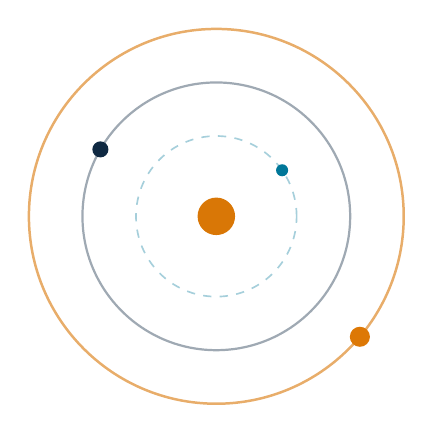
\begin{tikzpicture}[scale=0.85]
    \draw[orbitarCyanDark!35, line width=0.6pt, dashed] (0,0) circle (1.2cm);
    \draw[orbitarDeepBlue!40, line width=0.8pt] (0,0) circle (2.0cm);
    \draw[orbitarAmber!60, line width=0.9pt] (0,0) circle (2.8cm);
    \fill[orbitarAmber] (0,0) circle (0.28cm);
    \fill[orbitarCyanDark] (35:1.2cm) circle (0.09cm);
    \fill[orbitarDeepBlue] (150:2.0cm) circle (0.12cm);
    \fill[orbitarAmber!90!orange] (-40:2.8cm) circle (0.15cm);
  \end{tikzpicture}\\[0.8cm]
  {\color{orbitarDeepBlue}\large\itshape „Ad Astra — Prin Știință către Stele!”}\\[0.25cm]
  {\color{orbitarMuted}\small O călătorie enciclopedică prin cele trei orizonturi ale Universului:\\
  Sistemul Solar $\bullet$ Stele și Exoplanete $\bullet$ Nebuloase și Galaxii}
\end{center}
\vfill
\clearpage

% Pagina 5 PDF (v, Recto): Pagina de titlu interioară completă (Full Interior Title Page)
\thispagestyle{empty}
\vspace*{1.2cm}
\begin{center}
  {\color{orbitarCyanDark}\large\bfseries\scshape Planetariul Didactic Interactiv 3D}\\[0.45cm]
  {\color{orbitarDeepBlue}\fontsize{38}{44}\selectfont\bfseries ORBITAR}\\[0.4cm]
  {\color{orbitarAmber}\LARGE\bfseries Enciclopedia Cosmică Ilustrată}\\[0.5cm]
  
\begin{tikzpicture}
    \draw[orbitarDeepBlue, line width=1.2pt] (-5.5,0) -- (5.5,0);
    \draw[orbitarAmber, line width=0.8pt] (-3.8,-0.12) -- (3.8,-0.12);
  \end{tikzpicture}\\[0.5cm]
  {\color{orbitarDeepBlue}\large\bfseries Sistemul Solar $\bullet$ Sateliți Naturali $\bullet$ Planete Pitice și Asteroizi\\[4pt]
  Misiuni Spațiale, Sonde și Rovere $\bullet$ Stele și Exoplanete $\bullet$ Nebuloase și Galaxii}\\[0.45cm]
  {\color{orbitarMuted}\normalsize Prezentări enciclopedice detaliate, repere astrofizice esențiale, structură internă,\\
  istoric al explorării, hărți științifice, Laboratorul Orbitar și 66 de întrebări grilă cu barem}
\end{center}

\vfill

\begin{center}
  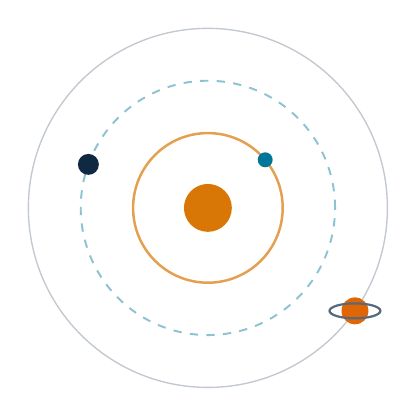
\begin{tikzpicture}[scale=0.95]
    \draw[orbitarDeepBlue!25, line width=0.5pt] (0,0) circle (2.4cm);
    \draw[orbitarCyanDark!45, line width=0.7pt, dashed] (0,0) circle (1.7cm);
    \draw[orbitarAmber!70, line width=0.9pt] (0,0) circle (1.0cm);
    \fill[orbitarAmber] (0,0) circle (0.32cm);
    \fill[orbitarCyanDark] (40:1.0cm) circle (0.10cm);
    \fill[orbitarDeepBlue] (160:1.7cm) circle (0.14cm);
    \fill[orbitarAmber!85!red] (-35:2.4cm) circle (0.18cm);
    \draw[orbitarDeepBlue!70, line width=0.8pt] (-35:2.4cm) ellipse (0.34cm and 0.10cm);
  \end{tikzpicture}
\end{center}

\vfill

\begin{center}
  \begin{tikzpicture}
    \draw[orbitarDeepBlue!40, line width=0.6pt] (-5.5,0) -- (5.5,0);
  \end{tikzpicture}\\[0.3cm]
  {\color{orbitarDeepBlue}\large\bfseries Proiectul Educațional Open-Source Orbitar (Ediția v1.2.9)}\\[4pt]
  {\color{orbitarMuted}\small Licență liberă GNU General Public License v3.0 (\texttt{GPL-3.0-or-later}) \quad$\bullet$\quad \texttt{https://orbitar.ro}}
\end{center}
\vspace*{0.5cm}
\clearpage

% Pagina 6 PDF (vi, Verso): Caseta tehnică, credite și licența GNU GPLv3
\thispagestyle{empty}
\vspace*{0.4cm}
\begin{tcolorbox}[orbitardata, title={\textbf{Caseta Tehnică a Cărții și Licența Liberă GNU GPLv3}}]
\textbf{Titlu:} \emph{Orbitar — Enciclopedia Cosmică Ilustrată: Sistemul Solar, Misiuni Spațiale, Exoplanete și Galaxii}\\[4pt]
\textbf{Baza de cunoștințe și redactare:} Informațiile, explicațiile didactice, analogiile și sintezele din această carte au fost agregate și redactate cu ajutorul inteligenței artificiale (AI) pe baza seturilor de date din aplicația \textbf{Orbitar v1.2.9} (\texttt{public/data/solar-system-ro.json}, \texttt{public/data/missions-ro.json}, \texttt{public/data/deep-space-ro.json}, \texttt{public/data/tle-iss.json} și modulele din \texttt{src/}).\\[4pt]
\textbf{Contribuitori proiect principal Orbitar:} Dragoș Iorgulescu (\texttt{@diorgulescu}), Google Antigravity (Gemini) \& Mistral Vibe.\\[4pt]
\textbf{Credite fotografii și hărți științifice:} NASA / JPL-Caltech / ESA / CSA / STScI (Telescoapele Spațiale Hubble, James Webb, Spitzer, GALEX, Euclid) / Event Horizon Telescope (EHT) / Solar Dynamics Observatory (SDO) / Lunar Reconnaissance Orbiter (LRO) / MOLA / MESSENGER / Magellan / Cassini-Huygens / Voyager 1 \& 2 / New Horizons / Dawn / Galileo / Viking / USGS Astrogeology (Public Domain \& CC-BY 4.0), CelestiaContent (GNU GPLv2+) \& Solar System Scope (CC-BY 4.0).\\[6pt]
\textbf{Licență — GNU General Public License v3.0 (\texttt{GPL-3.0-or-later}):}\\
Această carte (inclusiv codul sursă \LaTeX{}, scripturile de generare, diagramele vectoriale TikZ și ediția PDF rezultată) este o lucrare educațională liberă: o puteți copia, tipări, distribui în școli sau biblioteci și/sau modifica în conformitate cu termenii \textbf{Licenței Publice Generale GNU (GNU General Public License)} publicate de Free Software Foundation, fie versiunea 3 a Licenței, fie (la alegerea dumneavoastră) orice versiune ulterioară.\\[4pt]
Această lucrare este distribuită în speranța că va fi utilă elevilor, profesorilor și pasionaților de astronomie, dar \textbf{FĂRĂ NICIO GARANȚIE}, fără chiar garanția implicită de vandabilitate sau potrivire pentru un anumit scop. Consultați fișierul \texttt{LICENSE} din depozitul proiectului sau \url{https://www.gnu.org/licenses/gpl-3.0.html} pentru textul integral al licenței.
\end{tcolorbox}

\vspace{0.3cm}
\begin{tcolorbox}[orbitarlightyear, title={\textbf{Specificații Tehnice pentru Tipărire (Print-on-Demand / Blurb.com PDF-to-Book)}}]
\small
\textbf{Format și paginare:} A4 ($210 \times 297\text{ mm}$), paginare în oglindă (\texttt{twoside}, margine interioară de legătorie $24\text{ mm}$, margine exterioară $20\text{ mm}$).\\[2pt]
\textbf{Structură de tipar:} Documentul include Coperta I (față), paginile intermediare de gardă și de titlu la interior, blocul de carte cu capitolele ilustrate, colofonul tipografic, paginile de gardă finale (Coperta a III-a) și Coperta a IV-a (coperta-spate), numărul total de pagini fiind calibrat automat la multiplu de 4.
\end{tcolorbox}
\vfill
\clearpage

% Pagina 7 PDF (vii, Recto): Pagina de dedicație
\thispagestyle{empty}
\vspace*{7.0cm}
\begin{center}
  {\color{orbitarDeepBlue}\Large\itshape „Ad Astra — Prin Știință către Stele!”}\\[0.5cm]
  
\begin{tikzpicture}
    \draw[orbitarAmber, line width=0.8pt] (-2.5,0) -- (2.5,0);
  \end{tikzpicture}\\[0.5cm]
  \parbox{0.75\textwidth}{\centering\large\color{orbitarMuted}
  Dedicată tuturor copiilor curioși, elevilor, profesorilor și exploratorilor care privesc cerul înstelat și își pun întrebarea:\\[0.3cm]
  {\color{orbitarDeepBlue}\bfseries „Ce se află acolo, sus?”}}
\end{center}
\vfill
\clearpage

% Pagina 8 PDF (viii, Verso): Pagină intermediară albă înaintea Cuprinsului
\thispagestyle{empty}
\mbox{}
\clearpage

% Pagina 9 PDF (ix, Recto): Cuprinsul general
\tableofcontents

% Aliniere la multiplu de 4 pagini în frontmatter înaintea începerii blocului principal (\mainmatter)
\orbitarPadToModFour{1}

\mainmatter
% SPDX-License-Identifier: GPL-3.0-or-later
\chapter{Introducere în Universul Orbitar}
\label{chap:introducere}

\textbf{Orbitar} este un planetariu didactic interactiv 3D în limba română, conceput special pentru copiii cu vârste între \textbf{6 și 12 ani}, pentru orele de științe de la școală (la videoproiector sau tablă interactivă) și pentru explorarea cosmosului acasă. Această carte reunește, într-o formă enciclopedică ilustrată și tipăribilă, toate informațiile științifice, explicațiile pe înțelesul copiilor, analogiile vizuale, curiozitățile, istoricele misiunilor spațiale, laboratoarele interactive și întrebările de verificare din aplicația \textbf{Orbitar}.

\section{Cum este organizată această carte}

Fiecare dintre cele \textbf{66 de corpuri cerești, sateliți naturali, planete pitice, asteroizi, misiuni spațiale, stele, exoplanete, nebuloase și galaxii} din \textbf{Orbitar} este prezentat într-o formă enciclopedică unitară, prietenoasă dar riguroasă științific:

\begin{itemize}[leftmargin=1.5em, itemsep=4pt]
  \item \textbf{Ilustrații astronomice (glob 3D și planiglob desfășurat / fotografie oficială):} pentru toate corpurile din Sistemul Solar sunt afișate alături atât vederea tridimensională a corpului ceresc, cât și harta sa științifică desfășurată, iar pentru sonde, rovere, exoplanete, nebuloase și galaxii sunt incluse fotografiile oficiale NASA / ESA / JWST / Hubble / EHT.
  \item \textbf{Caseta cu repere esențiale:} o sinteză structurată sub formă de listă care reunește clasificarea, distanța de referință, raza, masa raportată la Pământ ($M_\oplus$), gravitația de suprafață ($g_\oplus$), perioada orbitală, rotația, temperatura medie, elementele kepleriene, durata călătoriei de pe Pământ (cu lumina, racheta, avionul și mașina) și analogia intuitivă de scară.
  \item \textbf{Descriere amplă în proză:} text narativ structurat pe trei direcții complementare (\emph{prezentarea generală și profilul astrofizic}, \emph{alcătuirea fizică și structura internă pe straturi} ori \emph{arhitectura tehnică și instrumentele științifice de la bord} în cazul sondelor, telescoapelor și roverelor, respectiv \emph{observațiile astronomice și istoricul explorării}), urmat de o întrebare grilă de verificare.
\end{itemize}

\section{Cele 3 Orizonturi Cosmice din Orbitar}

Universul este atât de vast încât nicio unitate de măsură unică nu poate descrie comod atât distanța de la Pământ la Stația Spațială Internațională (aproximativ $420\text{ de kilometri}$), cât și distanța până la Galaxia Sombrero ($29{,}3\text{ milioane de ani-lumină}$). De aceea, \textbf{Orbitar} (prin modulul \texttt{CosmicScaleNavigator}) organizează explorarea spațiului pe \textbf{3 Orizonturi Cosmice}:

\begin{center}
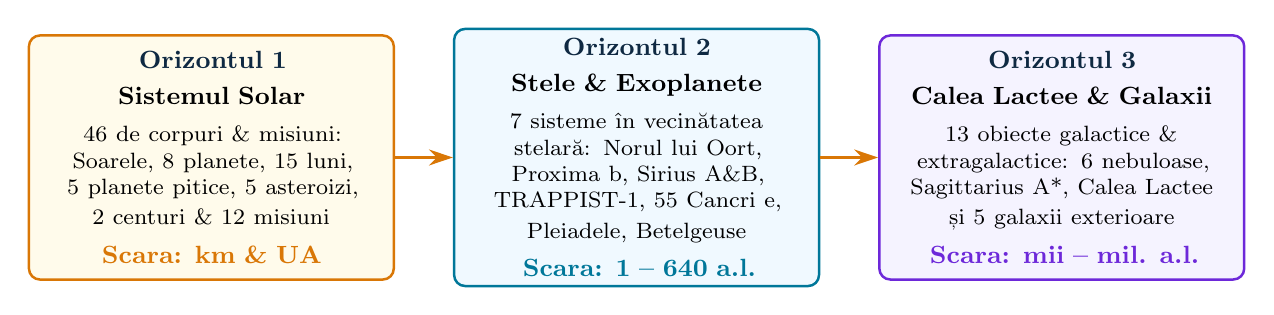
\begin{tikzpicture}[
  box/.style={rectangle, rounded corners=4pt, draw=orbitarDeepBlue, line width=0.9pt, fill=orbitarCadetBg, text width=4.4cm, minimum height=3.1cm, align=center, font=\small},
  arrow/.style={-{Stealth[length=3mm, width=2mm]}, line width=1.2pt, color=orbitarAmber}
]
  \node[box, fill=orbitarJuniorBg, draw=orbitarAmber] (h1) at (0,0) {
    \textbf{\color{orbitarDeepBlue}Orizontul 1}\\[2pt]
    \textbf{Sistemul Solar}\\[4pt]
    {\footnotesize 46 de corpuri \& misiuni:\\Soarele, 8 planete, 15 luni,\\5 planete pitice, 5 asteroizi,\\2 centuri \& 12 misiuni}\\[3pt]
    \textbf{\color{orbitarAmber}Scara: km \& UA}
  };

  \node[box, fill=orbitarCadetBg, draw=orbitarCyanDark] (h2) at (5.4,0) {
    \textbf{\color{orbitarDeepBlue}Orizontul 2}\\[2pt]
    \textbf{Stele \& Exoplanete}\\[4pt]
    {\footnotesize 7 sisteme în vecinătatea\\stelară: Norul lui Oort,\\Proxima b, Sirius A\&B,\\TRAPPIST-1, 55 Cancri e,\\Pleiadele, Betelgeuse}\\[3pt]
    \textbf{\color{orbitarCyanDark}Scara: 1 -- 640 a.l.}
  };

  \node[box, fill=orbitarQuizBg, draw=orbitarViolet] (h3) at (10.8,0) {
    \textbf{\color{orbitarDeepBlue}Orizontul 3}\\[2pt]
    \textbf{Calea Lactee \& Galaxii}\\[4pt]
    {\footnotesize 13 obiecte galactice \&\\extragalactice: 6 nebuloase,\\Sagittarius A*, Calea Lactee\\și 5 galaxii exterioare}\\[3pt]
    \textbf{\color{orbitarViolet}Scara: mii -- mil. a.l.}
  };

  \draw[arrow] (h1.east) -- (h2.west);
  \draw[arrow] (h2.east) -- (h3.west);
\end{tikzpicture}
\end{center}

\section{Unitățile de măsură ale astronomilor și scara didactică}

Pentru a înțelege cifrele din fișele tehnice ale cărții, iată reperele fundamentale folosite în \textbf{Orbitar}:

\begin{tcolorbox}[orbitardata, title={\textbf{Repere Fundamentale de Distanță, Timp și Gravitație în Orbitar}}]
\begin{itemize}[leftmargin=1.4em, itemsep=3pt]
  \item \textbf{Unitatea Astronomică ($1\text{ UA}$):} reprezintă distanța medie dintre Pământ și Soare, egală exact cu $149.597.870{,}7$ kilometri (aproximativ $150\text{ de milioane de kilometri}$). Planeta Mercur se află la $0{,}387\text{ UA}$, Pământul la $1{,}000\text{ UA}$, Jupiter la $5{,}204\text{ UA}$, Neptun la $30{,}07\text{ UA}$, iar planeta pitică Eris la $67{,}78\text{ UA}$.
  \item \textbf{Viteza Luminii ($1c$):} în vid, lumina și undele radio călătoresc cu $299.792{,}458$ kilometri pe secundă (aproximativ $300.000$ de kilometri pe secundă sau $1.079.252.848{,}8$ kilometri pe oră). O rază de lumină face $1{,}3\text{ secunde}$ de la Lună la Pământ și $8\text{ minute și } 20\text{ de secunde}$ de la Soare la Pământ.
  \item \textbf{Anul-Lumină (a.l.):} este o unitate de \textbf{distanță} (nu de timp!), egală cu drumul parcurs de o rază de lumină într-un an pământesc întreg: aproximativ $9.460\text{ de miliarde de kilometri}$ ($63.241\text{ UA}$).
  \item \textbf{Masa și Gravitația raportate la Pământ ($M_\oplus$ și $g_\oplus$):} Pământul are raza medie de $6.371$ de kilometri, accelerația gravitațională $1{,}00\,g_\oplus$ ($9{,}81\text{ m/s}^2$) și masa $1{,}00\,M_\oplus$ ($5{,}97 \times 10^{24}$ kilograme). Dacă o planetă are gravitația $0{,}38 \times g_\oplus$ (cum sunt Mercur și Marte), acolo vei cântări doar $38\%$ din greutatea de pe Pământ și vei putea sări de aproape trei ori mai sus!
  \item \textbf{Scară Didactică vs. Scară Reală:} în modul \emph{Scară Reală}, proporțiile dintre razele planetelor și distanțele în UA sunt cele fizice exacte (unde planetele par puncte minuscule în imensitatea spațiului). În modul \emph{Scară Didactică}, \textbf{Orbitar} mărește logaritmic corpurile și alocă culoare orbitale disjuncte pentru ca niciun satelit sau inel planetar să nu se intersecteze vizual cu planeta-mamă.
\end{itemize}
\end{tcolorbox}

\clearpage

% SPDX-License-Identifier: GPL-3.0-or-later
\chapter{Steaua Noastră, Planetele și Sateliții Lor Naturali}
\label{chap:planete}

Sistemul nostru Solar s-a format acum aproximativ \textbf{4,6 miliarde de ani} din prăbușirea gravitațională a unui nor molecular gigant de gaz și praf interstelar. Peste $99{,}86\%$ din întreaga masă a sistemului s-a concentrat în centru, dând naștere stelei noastre, \textbf{Soarele}, în timp ce din discul protoplanetar rămas s-au format \textbf{cele 8 planete majore} și \textbf{sateliții lor naturali (lunile)}, care sunt prezentate în acest capitol împreună cu planeta în jurul căreia orbitează:
\begin{enumerate}[leftmargin=1.6em, itemsep=2pt]
  \item \textbf{Planetele Interioare Telurice (Stâncoase):} \emph{Mercur} și \emph{Venus} (fără sateliți naturali), \emph{Pământul} (însoțit de \emph{Lună}) și \emph{Marte} (însoțit de sateliții săi capturați \emph{Phobos} și \emph{Deimos}).
  \item \textbf{Planetele Exterioare Gigante și Sistemele Lor de Sateliți:} \emph{Giganții Gazoși}, reprezentați de \emph{Jupiter} (cu cele 4 luni galileene: \emph{Io, Europa, Ganymede, Callisto}) și \emph{Saturn} (cu \emph{Mimas, Enceladus, Tethys, Dione, Rhea, Titan, Hyperion, Iapetus, Phoebe}), precum și \emph{Giganții de Gheață}, reprezentați de \emph{Uranus} (cu \emph{Miranda, Ariel, Umbriel, Titania, Oberon}) și \emph{Neptun} (cu satelitul retrograd \emph{Triton}).
\end{enumerate}

\begin{center}
\resizebox{\textwidth}{!}{%
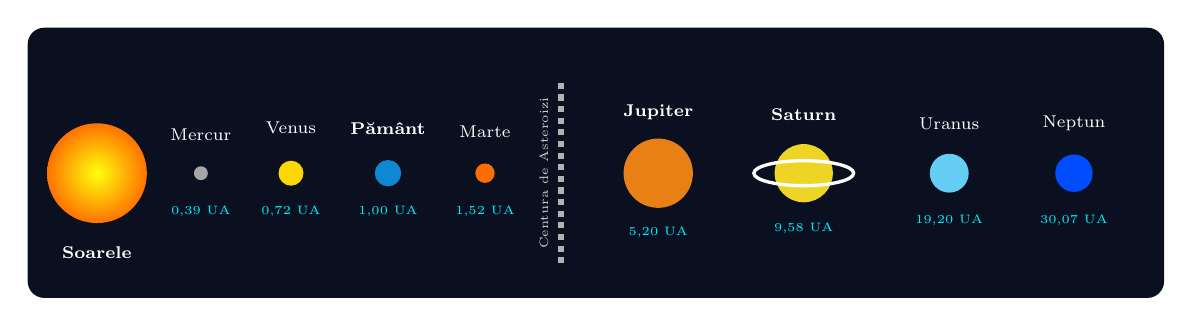
\begin{tikzpicture}[scale=0.88, every node/.style={transform shape}]
  \fill[orbitarSpaceBg, rounded corners=6pt] (-0.8,-1.8) rectangle (15.6,2.1);
  % Soarele
  \shade[inner color=yellow!95!white, outer color=orange!90!red] (0.2,0) circle (0.72cm);
  \node[white, font=\scriptsize\bfseries] at (0.2,-1.15) {Soarele};

  % Mercur
  \fill[gray!70] (1.7,0) circle (0.10cm);
  \node[white, font=\scriptsize] at (1.7,0.55) {Mercur};
  \node[orbitarCyan, font=\tiny] at (1.7,-0.55) {0,39 UA};

  % Venus
  \fill[yellow!75!orange] (3.0,0) circle (0.18cm);
  \node[white, font=\scriptsize] at (3.0,0.65) {Venus};
  \node[orbitarCyan, font=\tiny] at (3.0,-0.55) {0,72 UA};

  % Pământ
  \fill[cyan!70!blue] (4.4,0) circle (0.19cm);
  \node[white, font=\scriptsize\bfseries] at (4.4,0.65) {Pământ};
  \node[orbitarCyan, font=\tiny] at (4.4,-0.55) {1,00 UA};

  % Marte
  \fill[orange!85!red] (5.8,0) circle (0.14cm);
  \node[white, font=\scriptsize] at (5.8,0.60) {Marte};
  \node[orbitarCyan, font=\tiny] at (5.8,-0.55) {1,52 UA};

  % Centura de asteroizi
  \draw[gray!60, line width=2.2pt, dotted] (6.9,-1.3) -- (6.9,1.3);
  \node[gray!40, font=\tiny, rotate=90] at (6.65,0) {Centura de Asteroizi};

  % Jupiter
  \fill[orange!65!brown] (8.3,0) circle (0.50cm);
  \node[white, font=\scriptsize\bfseries] at (8.3,0.88) {Jupiter};
  \node[orbitarCyan, font=\tiny] at (8.3,-0.85) {5,20 UA};

  % Saturn
  \fill[yellow!70!brown] (10.4,0) circle (0.42cm);
  \draw[white!80, line width=1.2pt] (10.4,0) ellipse (0.72cm and 0.18cm);
  \node[white, font=\scriptsize\bfseries] at (10.4,0.85) {Saturn};
  \node[orbitarCyan, font=\tiny] at (10.4,-0.80) {9,58 UA};

  % Uranus
  \fill[cyan!60!white] (12.5,0) circle (0.28cm);
  \node[white, font=\scriptsize] at (12.5,0.72) {Uranus};
  \node[orbitarCyan, font=\tiny] at (12.5,-0.68) {19,20 UA};

  % Neptun
  \fill[blue!70!cyan] (14.3,0) circle (0.27cm);
  \node[white, font=\scriptsize] at (14.3,0.72) {Neptun};
  \node[orbitarCyan, font=\tiny] at (14.3,-0.68) {30,07 UA};
\end{tikzpicture}%
}
\end{center}

\begin{table}[H]
\centering
\small
\caption{Tabel sinoptic comparativ: Soarele și cele 8 planete ale Sistemului Solar în Orbitar}
\resizebox{\textwidth}{!}{%
\begin{tabular}{@{}llrrrrr@{}}
\toprule
\textbf{Corp ceresc} & \textbf{Clasă} & \textbf{Distanță (UA)} & \textbf{Rază (km)} & \textbf{Masă ($M_\oplus$)} & \textbf{Gravitație ($g_\oplus$)} & \textbf{Temp. medie} \\
\midrule
Soarele & Stea (G2V) & 0,00 & 696.340 & 332946,00 & 27,94 & 5.505$^\circ$C \\
Mercur & Telurică & 0,39 & 2.439,7 & 0,06 & 0,38 & 167$^\circ$C \\
Venus & Telurică & 0,72 & 6.051,8 & 0,81 & 0,90 & 464$^\circ$C \\
Pământul & Telurică & 1,00 & 6.371 & 1,00 & 1,00 & 15$^\circ$C \\
Marte & Telurică & 1,52 & 3.389,5 & 0,11 & 0,38 & -63$^\circ$C \\
Jupiter & Gigant gazos & 5,20 & 69.911 & 317,80 & 2,53 & -110$^\circ$C \\
Saturn & Gigant gazos & 9,58 & 58.232 & 95,16 & 1,06 & -140$^\circ$C \\
Uranus & Gigant gheață & 19,22 & 25.362 & 14,54 & 0,89 & -195$^\circ$C \\
Neptun & Gigant gheață & 30,11 & 24.622 & 17,15 & 1,14 & -200$^\circ$C \\
\bottomrule
\end{tabular}%
}
\end{table}

\begin{table}[H]
\centering
\small
\caption{Tabel sinoptic al celor 23 de sateliți naturali majori din Orbitar (asociați cu planetele lor)}
\resizebox{\textwidth}{!}{%
\begin{tabular}{@{}llrrrr@{}}
\toprule
\textbf{Satelit (Lună)} & \textbf{Planeta-mamă} & \textbf{Rază (km)} & \textbf{Gravitație ($g_\oplus$)} & \textbf{Perioadă orbitală} & \textbf{Temp. medie} \\
\midrule
Luna & Pământul & 1737,4 & 0,165 & 27,32 zile & -23$^\circ$C \\
Phobos & Marte & 11,3 & 0,001 & 0,32 zile & -40$^\circ$C \\
Deimos & Marte & 6,2 & 0,000 & 1,26 zile & -40$^\circ$C \\
Io & Jupiter & 1821,6 & 0,183 & 1,77 zile & -143$^\circ$C \\
Europa & Jupiter & 1560,8 & 0,134 & 3,55 zile & -160$^\circ$C \\
Ganymede & Jupiter & 2631,2 & 0,146 & 7,16 zile & -163$^\circ$C \\
Callisto & Jupiter & 2410,3 & 0,126 & 16,69 zile & -139$^\circ$C \\
Mimas & Saturn & 198,2 & 0,006 & 0,94 zile & -209$^\circ$C \\
Enceladus & Saturn & 252,1 & 0,011 & 1,37 zile & -198$^\circ$C \\
Tethys & Saturn & 531,1 & 0,015 & 1,89 zile & -187$^\circ$C \\
Dione & Saturn & 561,4 & 0,024 & 2,74 zile & -186$^\circ$C \\
Rhea & Saturn & 763,8 & 0,027 & 4,52 zile & -197$^\circ$C \\
Titan & Saturn & 2574,7 & 0,138 & 15,95 zile & -179$^\circ$C \\
Hyperion & Saturn & 135,0 & 0,002 & 21,28 zile & -180$^\circ$C \\
Iapetus & Saturn & 734,5 & 0,023 & 79,32 zile & -163$^\circ$C \\
Phoebe & Saturn & 106,5 & 0,004 & 550,31 zile (retrograd) & -198$^\circ$C \\
Miranda & Uranus & 235,8 & 0,008 & 1,41 zile & -213$^\circ$C \\
Ariel & Uranus & 578,9 & 0,025 & 2,52 zile & -213$^\circ$C \\
Umbriel & Uranus & 584,7 & 0,023 & 4,14 zile & -198$^\circ$C \\
Titania & Uranus & 788,4 & 0,039 & 8,71 zile & -203$^\circ$C \\
Oberon & Uranus & 761,4 & 0,035 & 13,46 zile & -198$^\circ$C \\
Triton & Neptun & 1353,4 & 0,079 & 5,88 zile (retrograd) & -235$^\circ$C \\
Charon & Pluto & 606,0 & 0,029 & 6,39 zile & -220$^\circ$C \\
\bottomrule
\end{tabular}%
}
\end{table}

\clearpage

\section{Soarele}
\label{sec:body-sun}
\vspace{-4pt}
{\large\itshape\color{orbitarAccent} Steaua centrală a Sistemului Solar (Pitică Galbenă G2V)}\\[4pt]


\begin{center}
\begin{tabular}{@{}m{0.44\textwidth}@{\hspace{0.03\textwidth}}m{0.51\textwidth}@{}}
\centering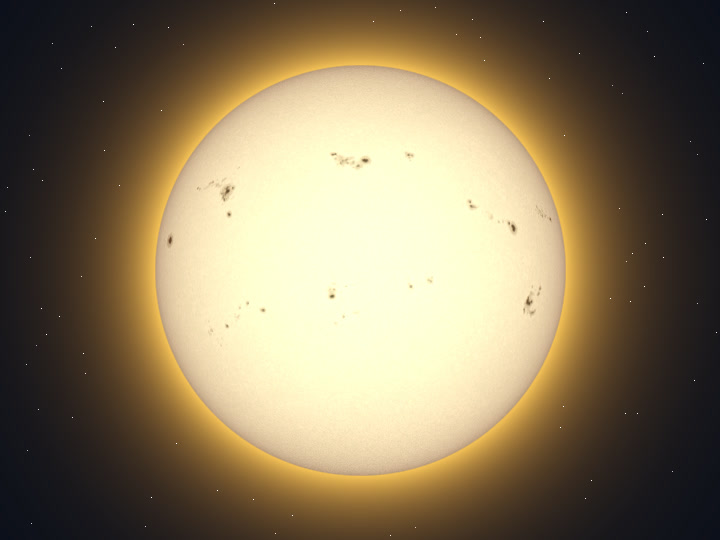
\includegraphics[width=\linewidth,height=4.4cm,keepaspectratio]{imagini/globuri/sun.jpg}\\[2pt]
{\scriptsize\itshape\color{orbitarMuted} Vedere 3D a corpului ceresc (\textbf{Soarele})}
&
\centering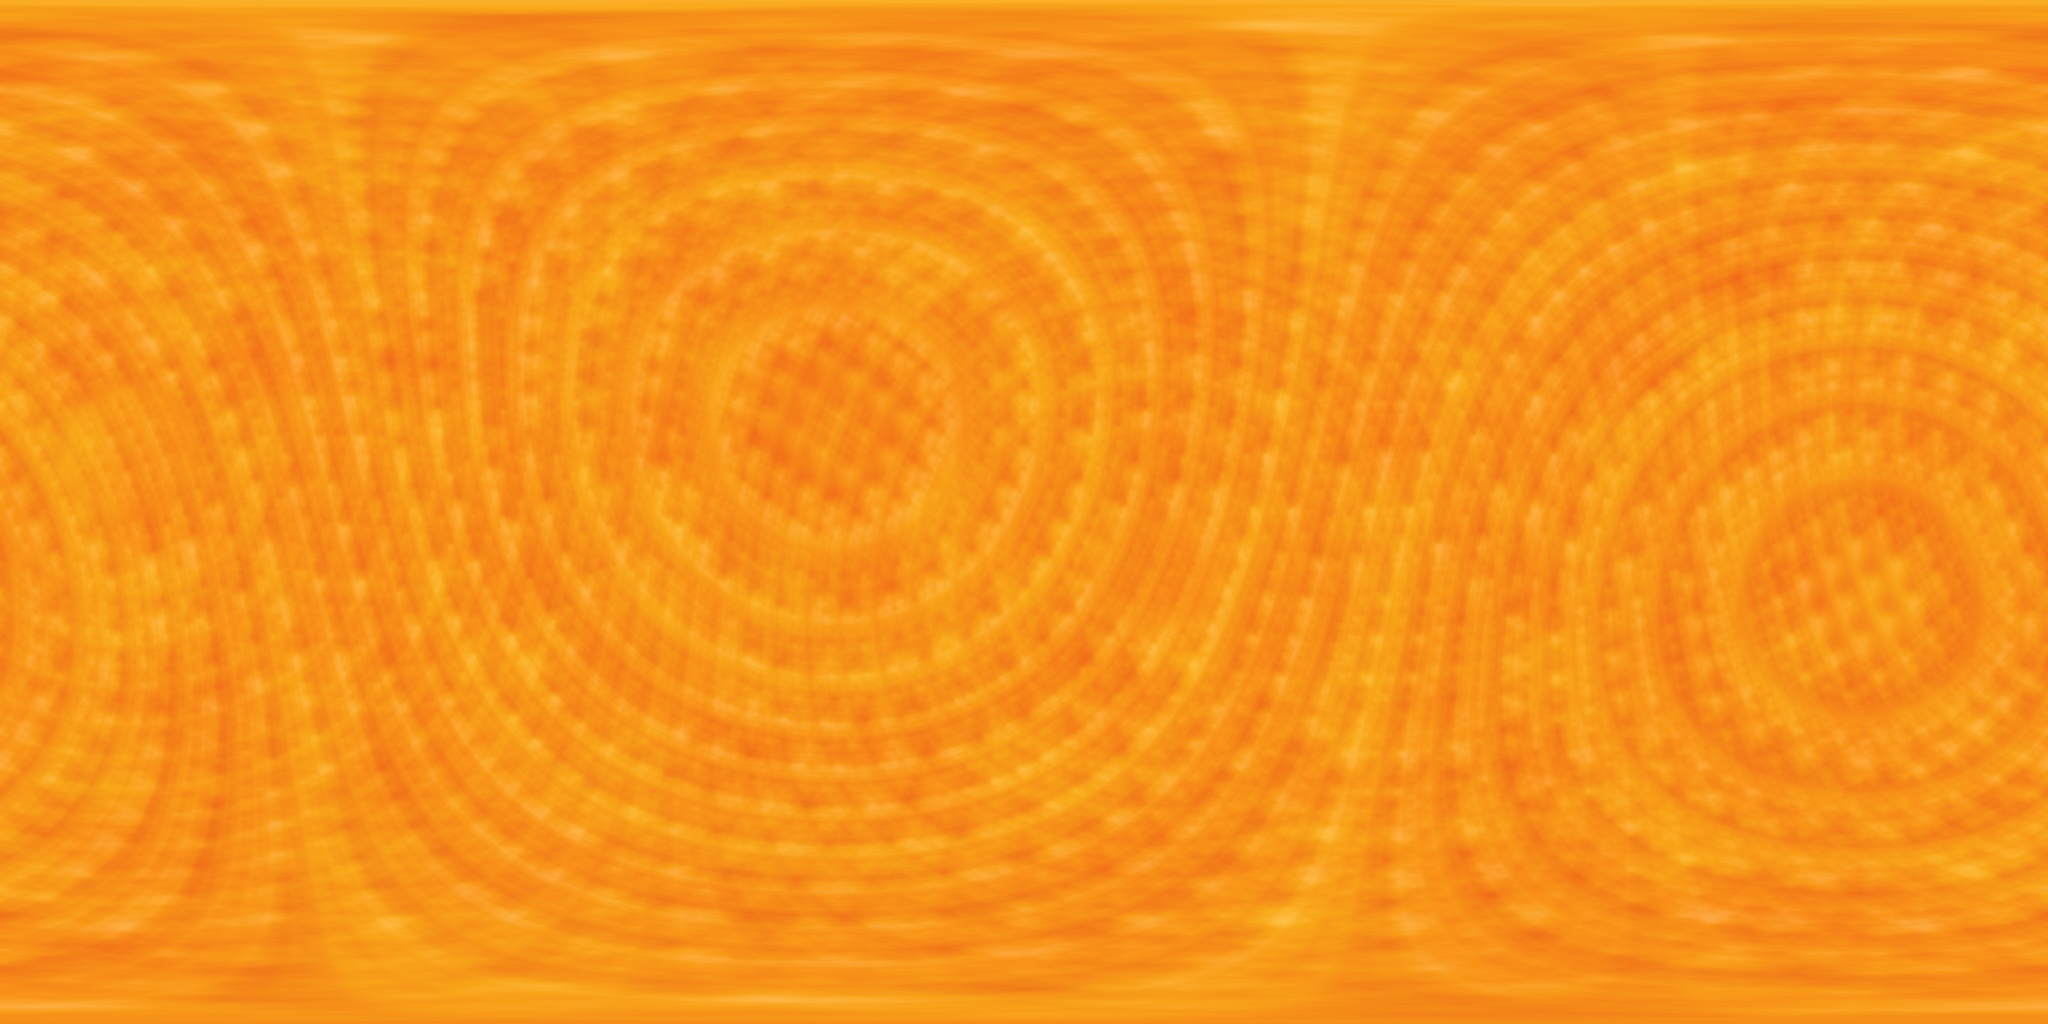
\includegraphics[width=\linewidth,height=4.4cm,keepaspectratio]{../public/textures/hd/sun_albedo.jpg}\\[2pt]
{\scriptsize\itshape\color{orbitarMuted} Planiglob desfășurat: Harta fotosferei solare în rezoluție 2K folosită în Orbitar (date NASA Solar Dynamics Observatory, SDO).}
\end{tabular}
\end{center}


\begin{tcolorbox}[orbitardata, title={\textbf{Repere esențiale: Soarele}}]
\small
\begin{itemize}[leftmargin=1.4em, itemsep=2pt, topsep=2pt]
  \item \textbf{Clasificare și orbită:} Stea \quad$\bullet$\quad \textbf{Distanță:} 0 UA (Centrul Sistemului Solar)
  \item \textbf{Dimensiuni și masă:} rază medie 696.340 de kilometri \quad$\bullet$\quad masă: 332946,000 $\times M_\oplus$
  \item \textbf{Gravitație și regim termic:} 27,940 $\times g_\oplus$ (274,09 m/s$^2$) \quad$\bullet$\quad temperatură medie: +5.505 $^\circ$C (înclinarea axei: 7,25$^\circ$)
  \item \textbf{Ciclu orbital și rotație:} perioadă orbitală (an): Orbitează centrul Căii Lactee (aproximativ 230 de milioane de ani) \quad$\bullet$\quad rotație (zi): 609,12 ore (25,38 zile pământești)
  \item \textbf{Durata călătoriei de pe Pământ:} cu viteza luminii ($1c$): \emph{8 minute și 20 de secunde}; cu racheta ($50.000$ de kilometri pe oră): \emph{4 luni cu o navă spațială rapidă}; cu avionul ($900$ de kilometri pe oră): \emph{19 ani cu un avion de pasageri}; cu mașina ($100$ de kilometri pe oră): \emph{171 de ani (fără oprire, cu 100 kilometri pe oră)}.
  \item \textbf{Repere de scară și curiozitate:} Dacă Soarele ar fi cât o minge mare de plajă, Pământul ar fi doar cât un bob mic de mazăre! În interiorul Soarelui ar încăpea aproximativ 1,3 milioane de planete Pământ!
\end{itemize}
\end{tcolorbox}

\subsubsection*{Prezentare generală și profil astrofizic}
Soarele este o stea de tip spectral G2V care concentrează 99,86\% din masa totală a Sistemului Solar. În nucleul său, la temperaturi de 15 milioane $^\circ$C, fuziunea nucleară transformă 600 de milioane de tone de hidrogen în heliu în fiecare secundă. Soarele este o minge uriașă de foc și plasmă strălucitoare care ne dă lumină și căldură în fiecare zi. Fără el, pe Pământ ar fi întuneric și un frig de gheață! Dacă Soarele ar fi cât o minge mare de plajă, Pământul ar fi doar cât un bob mic de mazăre!

\subsubsection*{Alcătuirea fizică și structura internă}
Privind în profunzimea sa, alcătuirea fizică este organizată pe mai multe straturi și regiuni distincte, fiecare având un rol bine definit în evoluția și dinamica acestui obiect cosmic. În primul rând se remarcă \textbf{Nucleul solar}, zona centrală extrem de densă (15.000.000 $^\circ$C) unde au loc reacțiile de fuziune proton-proton. În strânsă legătură cu această componentă se află \textbf{Zona radiativă și convectivă}, straturile prin care fotonii și curenții de plasmă transportă energia spre suprafață timp de mii de ani. În completarea acestui ansamblu întâlnim \textbf{Fotosfera și Coroana}, suprafața vizibilă la 5.505 $^\circ$C și atmosfera exterioară rarefiată care depășește 1.000.000 $^\circ$C.

\subsubsection*{Observații astronomice și istoricul explorării}
Studiat de misiunile SOHO, Solar Dynamics Observatory (SDO), Solar Orbiter (ESA) și Parker Solar Probe (NASA), care a pătruns direct în coroana solară. În interiorul Soarelui ar încăpea aproximativ 1,3 milioane de planete Pământ!

\vspace{6pt}
\begin{tcolorbox}[orbitarquiz, title={\textbf{Întrebare de verificare \#1: Soarele}}]
\textbf{Ce procent din masa întregului Sistem Solar se află în Soare?}
\begin{itemize}[leftmargin=2.2em, itemsep=2pt, topsep=4pt]
  \item[$\square$ \textbf{A.}] Aproximativ 50\%
  \item[$\square$ \textbf{B.}] Aproximativ 75\%
  \item[$\square$ \textbf{C.}] Peste 99,8\%
  \item[$\square$ \textbf{D.}] Sub 25\%
\end{itemize}
\vspace{2pt}
{\footnotesize\color{orbitarMuted}\textbf{Răspuns corect:} \textbf{C} (Peste 99,8\%). \emph{Soarele concentrează 99,86\% din masa Sistemului Solar; toate planetele, lunile și asteroizii la un loc reprezintă doar 0,14\%!}}
\end{tcolorbox}
\clearpage


\section{Mercur}
\label{sec:body-mercury}
\vspace{-4pt}
{\large\itshape\color{orbitarAccent} Cea mai apropiată și mai mică planetă de la Soare}\\[4pt]


\begin{center}
\begin{tabular}{@{}m{0.44\textwidth}@{\hspace{0.03\textwidth}}m{0.51\textwidth}@{}}
\centering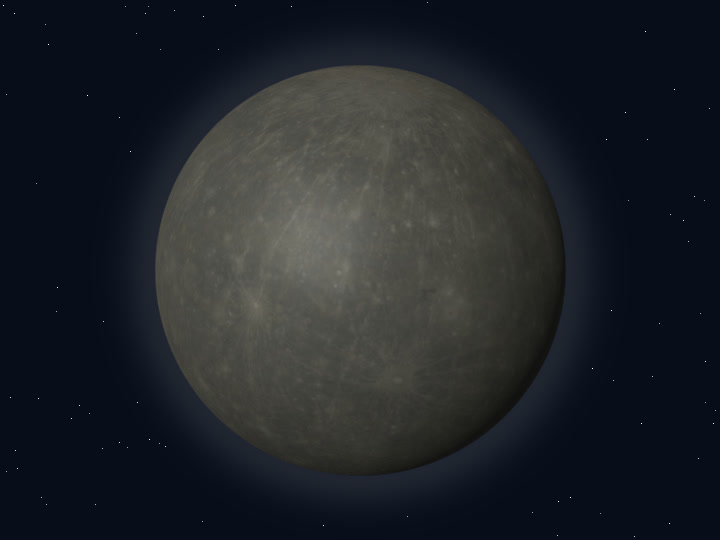
\includegraphics[width=\linewidth,height=4.4cm,keepaspectratio]{imagini/globuri/mercury.jpg}\\[2pt]
{\scriptsize\itshape\color{orbitarMuted} Vedere 3D a corpului ceresc (\textbf{Mercur})}
&
\centering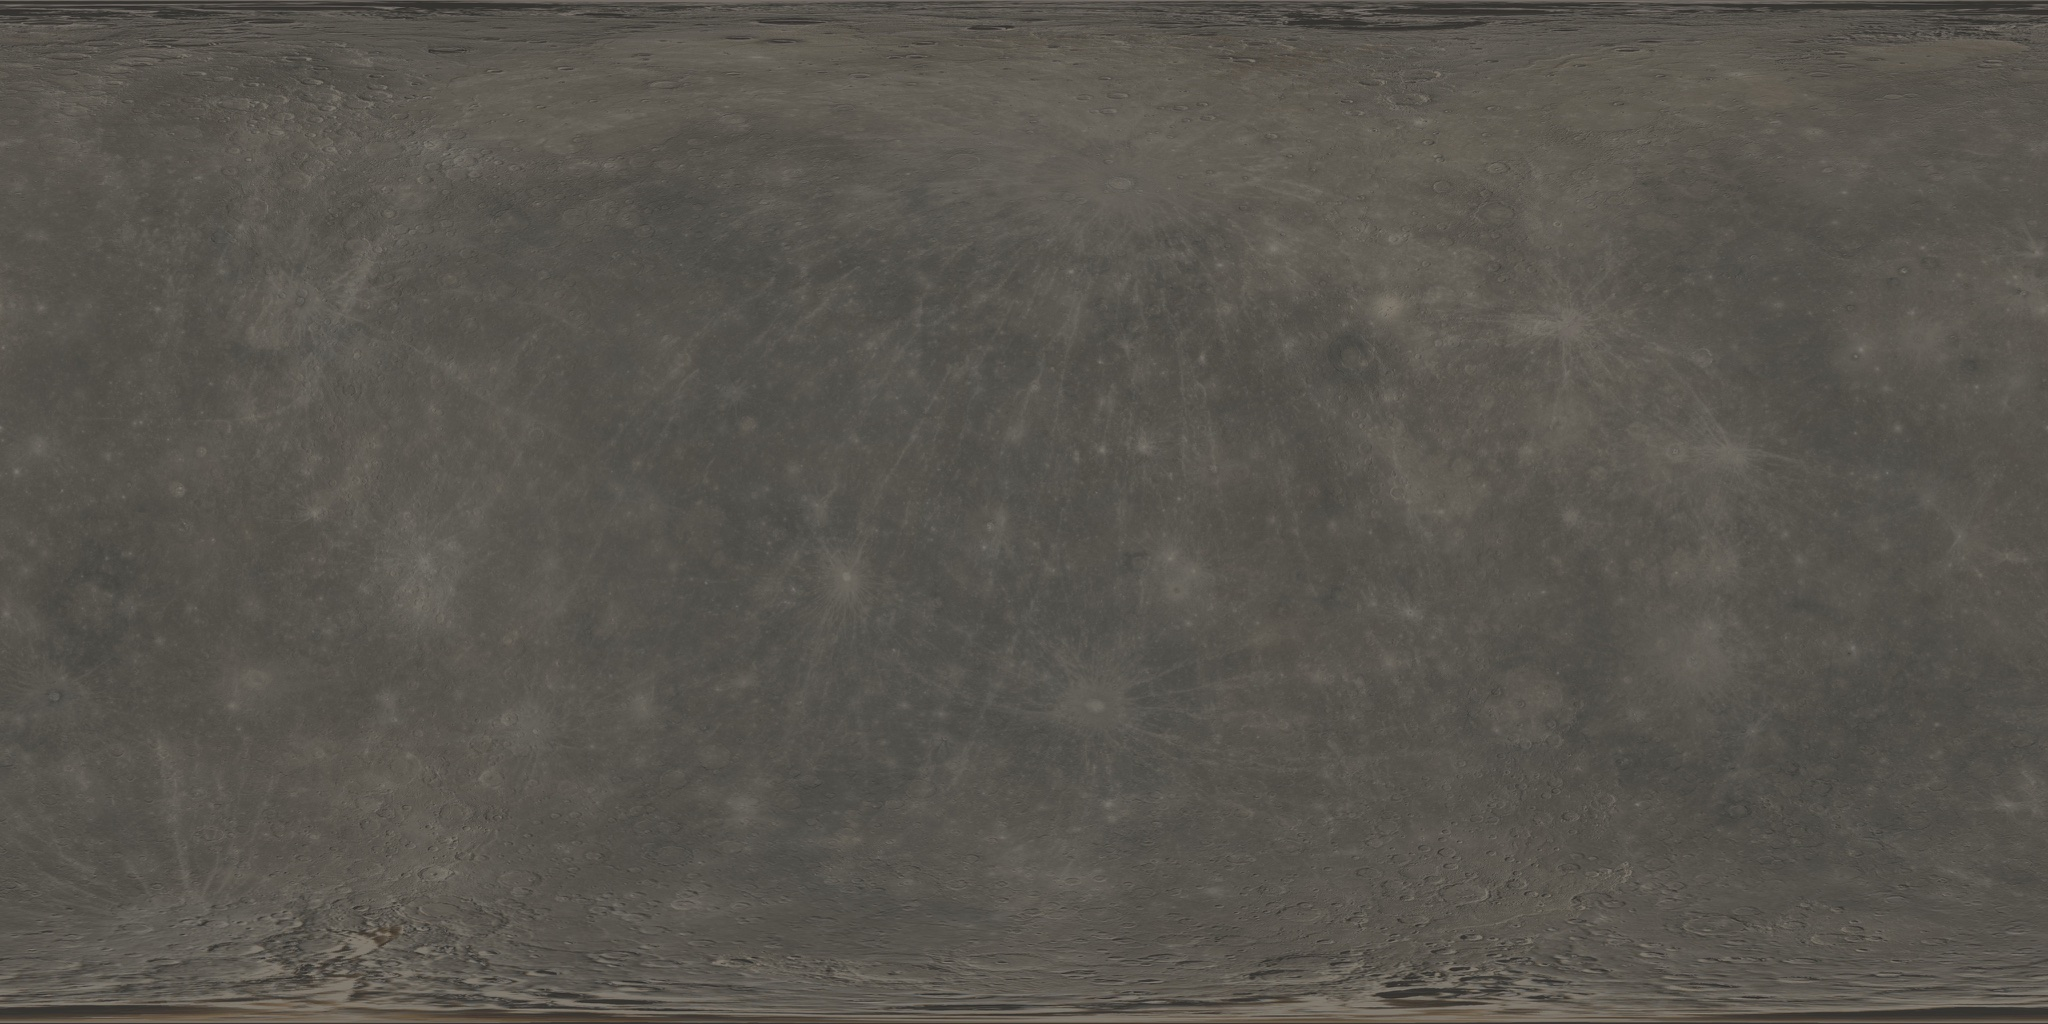
\includegraphics[width=\linewidth,height=4.4cm,keepaspectratio]{../public/textures/hd/mercury_messenger_albedo.jpg}\\[2pt]
{\scriptsize\itshape\color{orbitarMuted} Planiglob desfășurat: Harta globală a suprafeței craterizate a lui Mercur, realizată de sonda NASA MESSENGER (2K HD).}
\end{tabular}
\end{center}


\begin{tcolorbox}[orbitardata, title={\textbf{Repere esențiale: Mercur}}]
\small
\begin{itemize}[leftmargin=1.4em, itemsep=2pt, topsep=2pt]
  \item \textbf{Clasificare și orbită:} Planetă Telurică (Stâncoasă) \quad$\bullet$\quad \textbf{Distanță:} 0,387 UA ($\approx$ 58 milioane de kilometri)
  \item \textbf{Dimensiuni și masă:} rază medie 2.439,7 de kilometri \quad$\bullet$\quad masă: 0,055 $\times M_\oplus$
  \item \textbf{Gravitație și regim termic:} 0,380 $\times g_\oplus$ (3,73 m/s$^2$) \quad$\bullet$\quad temperatură medie: +167 $^\circ$C (înclinarea axei: 0,03$^\circ$)
  \item \textbf{Ciclu orbital și rotație:} perioadă orbitală (an): 87,97 zile pământești \quad$\bullet$\quad rotație (zi): 1407,60 ore (58,65 zile pământești)
  \item \textbf{Durata călătoriei de pe Pământ:} cu viteza luminii ($1c$): \emph{5 minute de pe Pământ}; cu racheta ($50.000$ de kilometri pe oră): \emph{3 luni}; cu avionul ($900$ de kilometri pe oră): \emph{11 ani și jumătate}; cu mașina ($100$ de kilometri pe oră): \emph{105 ani}.
  \item \textbf{Repere de scară și curiozitate:} Mercur este doar puțin mai mare decât Luna noastră și arată aproape ca o nucă cenușie plină de gropițe. Deși este cel mai aproape de Soare, noaptea pe Mercur îngheață totul la -180 $^\circ$C pentru că nu are o pătură de aer!
\end{itemize}
\end{tcolorbox}

\subsubsection*{Prezentare generală și profil astrofizic}
Mercur este o planetă telurică densă, având un nucleu metalic uriaș din fier care ocupă 85\% din raza planetei. Lipsa unei atmosfere substanțiale (are doar o exosferă subțire) provoacă cele mai mari variații termice din Sistemul Solar. Mercur este mesagerul rapid al Sistemului Solar! Fiind cel mai aproape de Soare, termină o tură completă în doar 88 de zile. Mercur este doar puțin mai mare decât Luna noastră și arată aproape ca o nucă cenușie plină de gropițe.

\subsubsection*{Alcătuirea fizică și structura internă}
Privind în profunzimea sa, alcătuirea fizică este organizată pe mai multe straturi și regiuni distincte, fiecare având un rol bine definit în evoluția și dinamica acestui obiect cosmic. În primul rând se remarcă \textbf{Nucleu metalic supradimensionat}, format din fier solid și lichid, reprezintă aproximativ 85\% din raza planetei și generează un câmp magnetic propriu. În strânsă legătură cu această componentă se află \textbf{Manta silicatată subțire}, un înveliș de roci de numai 400 de kilometri grosime. În completarea acestui ansamblu întâlnim \textbf{Scoarță craterizată}, dominată de Bazinul Caloris (1.550 de kilometri diametru) și faleze de contracție numite rupes.

\subsubsection*{Observații astronomice și istoricul explorării}
Vizitată de Mariner 10 (1974--1975), cartografiată complet de sonda MESSENGER (2011--2015) și explorată de misiunea europeo-japoneză BepiColombo. Deși este cel mai aproape de Soare, noaptea pe Mercur îngheață totul la -180 $^\circ$C pentru că nu are o pătură de aer!

\vspace{6pt}
\begin{tcolorbox}[orbitarquiz, title={\textbf{Întrebare de verificare \#2: Mercur}}]
\textbf{Cât durează un an pe planeta Mercur (o orbită completă în jurul Soarelui)?}
\begin{itemize}[leftmargin=2.2em, itemsep=2pt, topsep=4pt]
  \item[$\square$ \textbf{A.}] 365 de zile
  \item[$\square$ \textbf{B.}] 88 de zile pământești
  \item[$\square$ \textbf{C.}] 24 de ore
  \item[$\square$ \textbf{D.}] 12 ani
\end{itemize}
\vspace{2pt}
{\footnotesize\color{orbitarMuted}\textbf{Răspuns corect:} \textbf{B} (88 de zile pământești). \emph{Fiind cea mai apropiată planetă de Soare, Mercur parcurge orbita cu aproximativ 47 kilometri pe secundă și încheie un an în doar 88 de zile terestre.}}
\end{tcolorbox}
\clearpage


\section{Venus}
\label{sec:body-venus}
\vspace{-4pt}
{\large\itshape\color{orbitarAccent} Luceafărul strălucitor cu efect de seră extrem}\\[4pt]


\begin{center}
\begin{tabular}{@{}m{0.44\textwidth}@{\hspace{0.03\textwidth}}m{0.51\textwidth}@{}}
\centering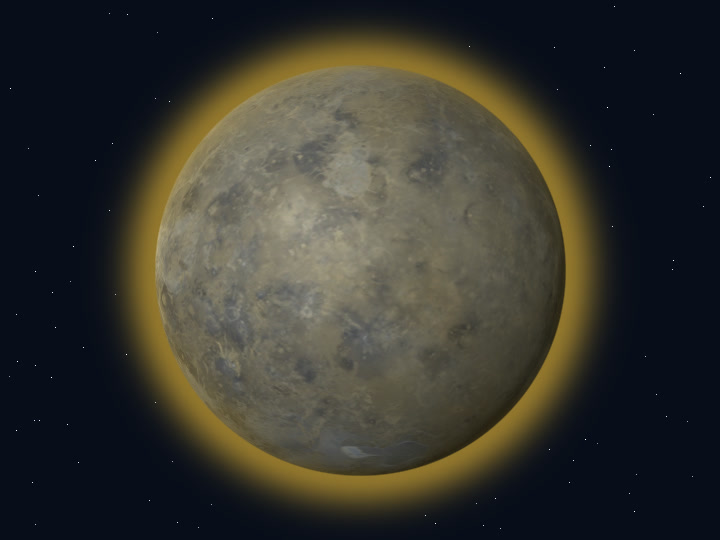
\includegraphics[width=\linewidth,height=4.4cm,keepaspectratio]{imagini/globuri/venus.jpg}\\[2pt]
{\scriptsize\itshape\color{orbitarMuted} Vedere 3D a corpului ceresc (\textbf{Venus})}
&
\centering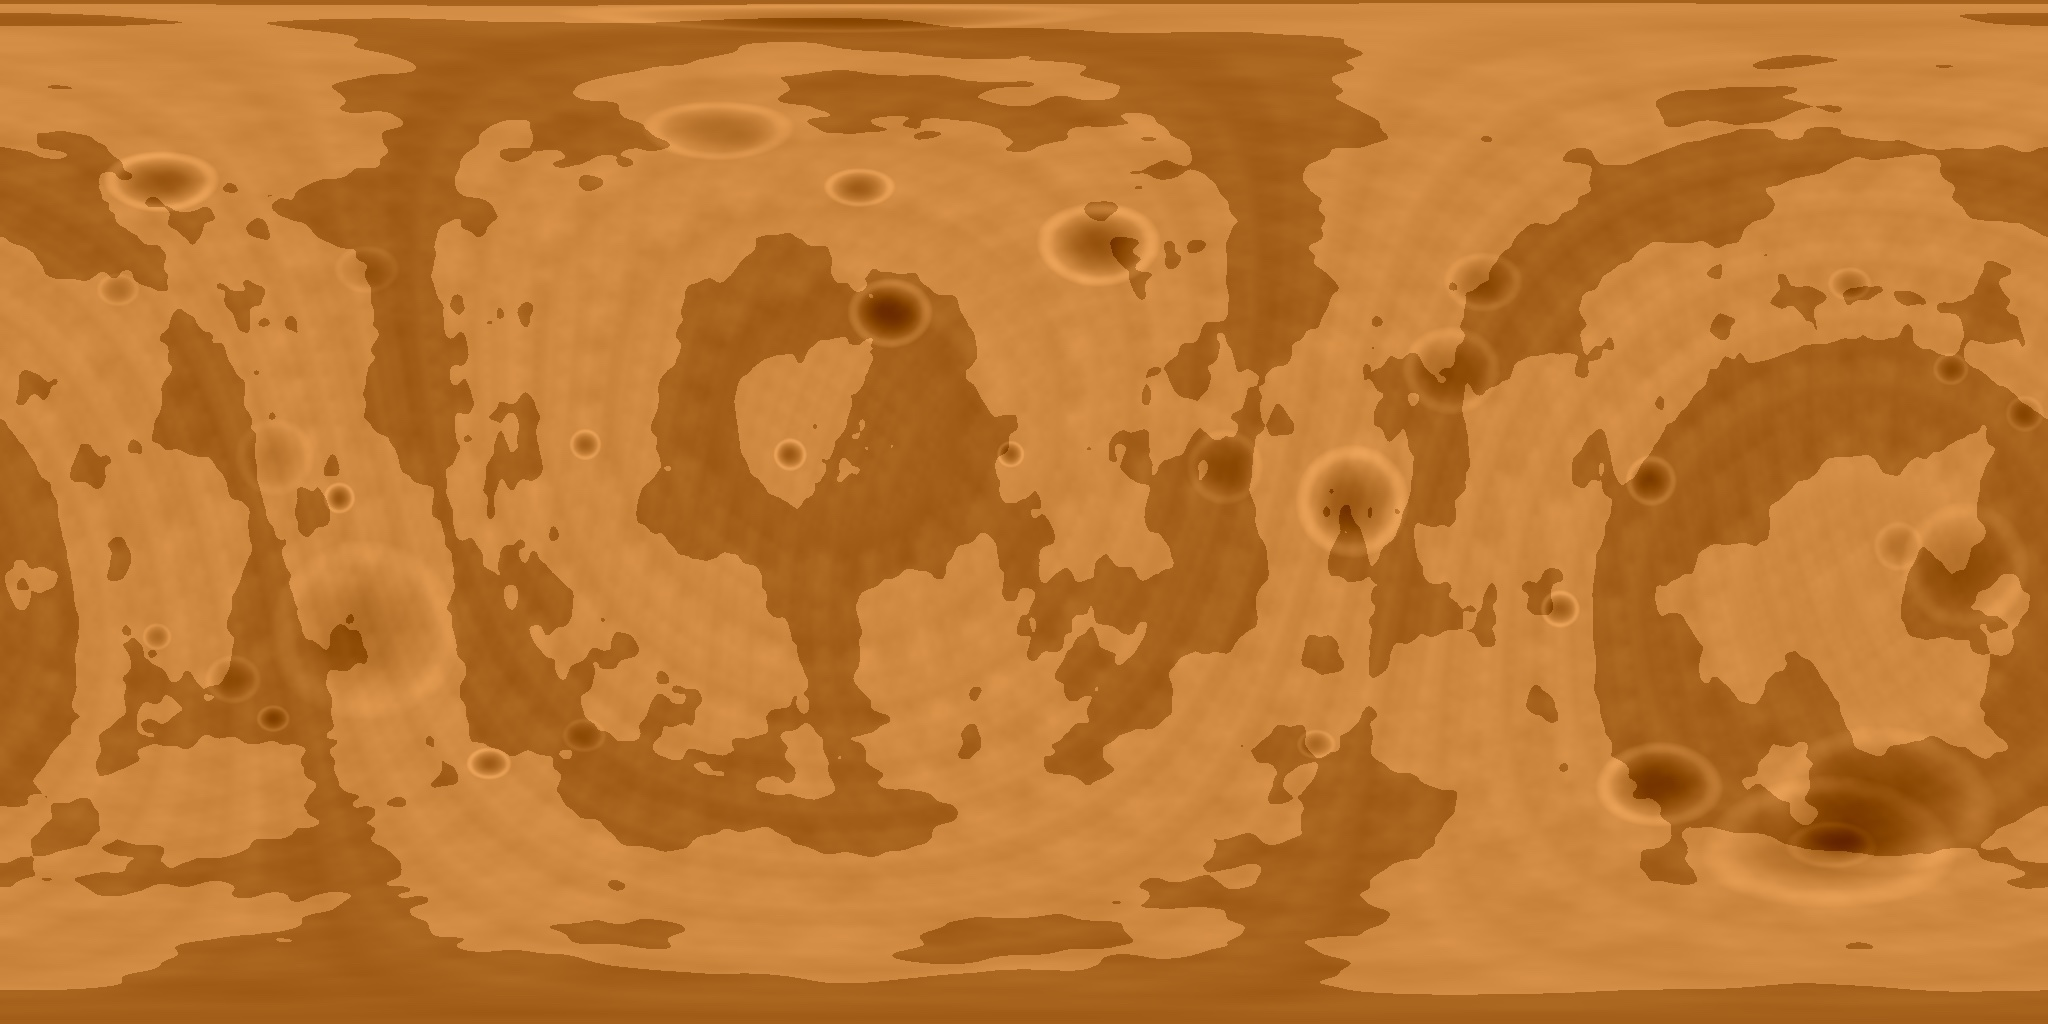
\includegraphics[width=\linewidth,height=4.4cm,keepaspectratio]{../public/textures/hd/venus_magellan_surface.jpg}\\[2pt]
{\scriptsize\itshape\color{orbitarMuted} Planiglob desfășurat: Harta radar a reliefului vulcanic de sub norii planetei Venus, obținută de sonda NASA Magellan (modul \quotedblbase{}Vezi sub nori\textquotedblright{} în Orbitar).}
\end{tabular}
\end{center}


\begin{tcolorbox}[orbitardata, title={\textbf{Repere esențiale: Venus}}]
\small
\begin{itemize}[leftmargin=1.4em, itemsep=2pt, topsep=2pt]
  \item \textbf{Clasificare și orbită:} Planetă Telurică (Stâncoasă) \quad$\bullet$\quad \textbf{Distanță:} 0,723 UA ($\approx$ 108 milioane de kilometri)
  \item \textbf{Dimensiuni și masă:} rază medie 6.051,8 de kilometri \quad$\bullet$\quad masă: 0,815 $\times M_\oplus$
  \item \textbf{Gravitație și regim termic:} 0,900 $\times g_\oplus$ (8,83 m/s$^2$) \quad$\bullet$\quad temperatură medie: +464 $^\circ$C (înclinarea axei: 177,36$^\circ$)
  \item \textbf{Ciclu orbital și rotație:} perioadă orbitală (an): 224,7 zile pământești \quad$\bullet$\quad rotație (zi): 5832,50 ore (Rotație retrogradă!)
  \item \textbf{Durata călătoriei de pe Pământ:} cu viteza luminii ($1c$): \emph{2 minute și 18 secunde}; cu racheta ($50.000$ de kilometri pe oră): \emph{3 luni și jumătate}; cu avionul ($900$ de kilometri pe oră): \emph{5 ani și 2 luni}; cu mașina ($100$ de kilometri pe oră): \emph{47 de ani (când este cel mai aproape)}.
  \item \textbf{Repere de scară și curiozitate:} Venus are aproape aceeași mărime ca Pământul, asemenea a două portocale așezate una lângă alta! Pe Venus, Soarele răsare din vest și apune în est, deoarece planeta se învârte invers față de Pământ!
\end{itemize}
\end{tcolorbox}

\subsubsection*{Prezentare generală și profil astrofizic}
Numită sora geamănă a Pământului datorită dimensiunii și masei similare, Venus are o atmosferă compusă în proporție de 96,5\% din dioxid de carbon, cu o presiune la sol de 92 de ori mai mare decât cea terestră. Venus este cel mai strălucitor obiect de pe cerul nopții după Lună! Este învelită în nori groși și gălbui care păstrează căldura ca într-un cuptor. Venus are aproape aceeași mărime ca Pământul, asemenea a două portocale așezate una lângă alta!

\subsubsection*{Alcătuirea fizică și structura internă}
Privind în profunzimea sa, alcătuirea fizică este organizată pe mai multe straturi și regiuni distincte, fiecare având un rol bine definit în evoluția și dinamica acestui obiect cosmic. În primul rând se remarcă \textbf{Nucleu de fier și nichel}, similar cu cel terestru, dar fără efectul de dinam magnetic din cauza rotației extrem de lente. În strânsă legătură cu această componentă se află \textbf{Manta și scoarță vulcanică}, peste 1.600 de vulcani majori, platouri ca Ishtar Terra și munții Maxwell Montes. În completarea acestui ansamblu întâlnim \textbf{Atmosferă super-densă}, nori de acid sulfuric și CO$_2$ care mențin temperatura medie la +464 $^\circ$C.

\subsubsection*{Observații astronomice și istoricul explorării}
Sondele sovietice Venera au reușit primele asolizări și fotografii de pe suprafață (1970--1982), iar sonda NASA Magellan a cartografiat relieful prin radar. Pe Venus, Soarele răsare din vest și apune în est, deoarece planeta se învârte invers față de Pământ!

\vspace{6pt}
\begin{tcolorbox}[orbitarquiz, title={\textbf{Întrebare de verificare \#3: Venus}}]
\textbf{De ce este Venus mai fierbinte decât Mercur, deși se află mai departe de Soare?}
\begin{itemize}[leftmargin=2.2em, itemsep=2pt, topsep=4pt]
  \item[$\square$ \textbf{A.}] Are mai mulți vulcani activi
  \item[$\square$ \textbf{B.}] Are o atmosferă densă de CO$_2$ care creează un efect de seră extrem
  \item[$\square$ \textbf{C.}] Este mai mare decât Mercur
  \item[$\square$ \textbf{D.}] Se rotește foarte repede
\end{itemize}
\vspace{2pt}
{\footnotesize\color{orbitarMuted}\textbf{Răspuns corect:} \textbf{B} (Are o atmosferă densă de CO$_2$ care creează un efect de seră extrem). \emph{Atmosfera groasă de dioxid de carbon captează radiația termică, ridicând temperatura la +464 $^\circ$C pe toată suprafața planetei.}}
\end{tcolorbox}
\clearpage


\section{Pământul}
\label{sec:body-earth}
\vspace{-4pt}
{\large\itshape\color{orbitarAccent} Planeta Albastră, singura lume cunoscută care găzduiește viață}\\[4pt]


\begin{center}
\begin{tabular}{@{}m{0.44\textwidth}@{\hspace{0.03\textwidth}}m{0.51\textwidth}@{}}
\centering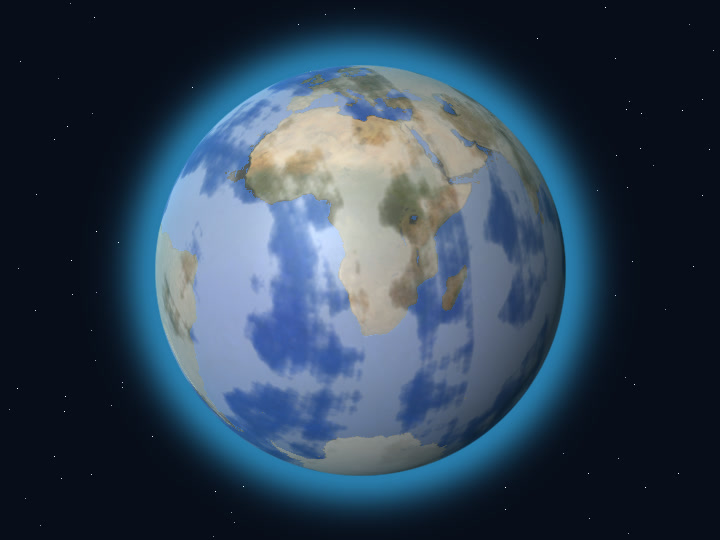
\includegraphics[width=\linewidth,height=4.4cm,keepaspectratio]{imagini/globuri/earth.jpg}\\[2pt]
{\scriptsize\itshape\color{orbitarMuted} Vedere 3D a corpului ceresc (\textbf{Pământul})}
&
\centering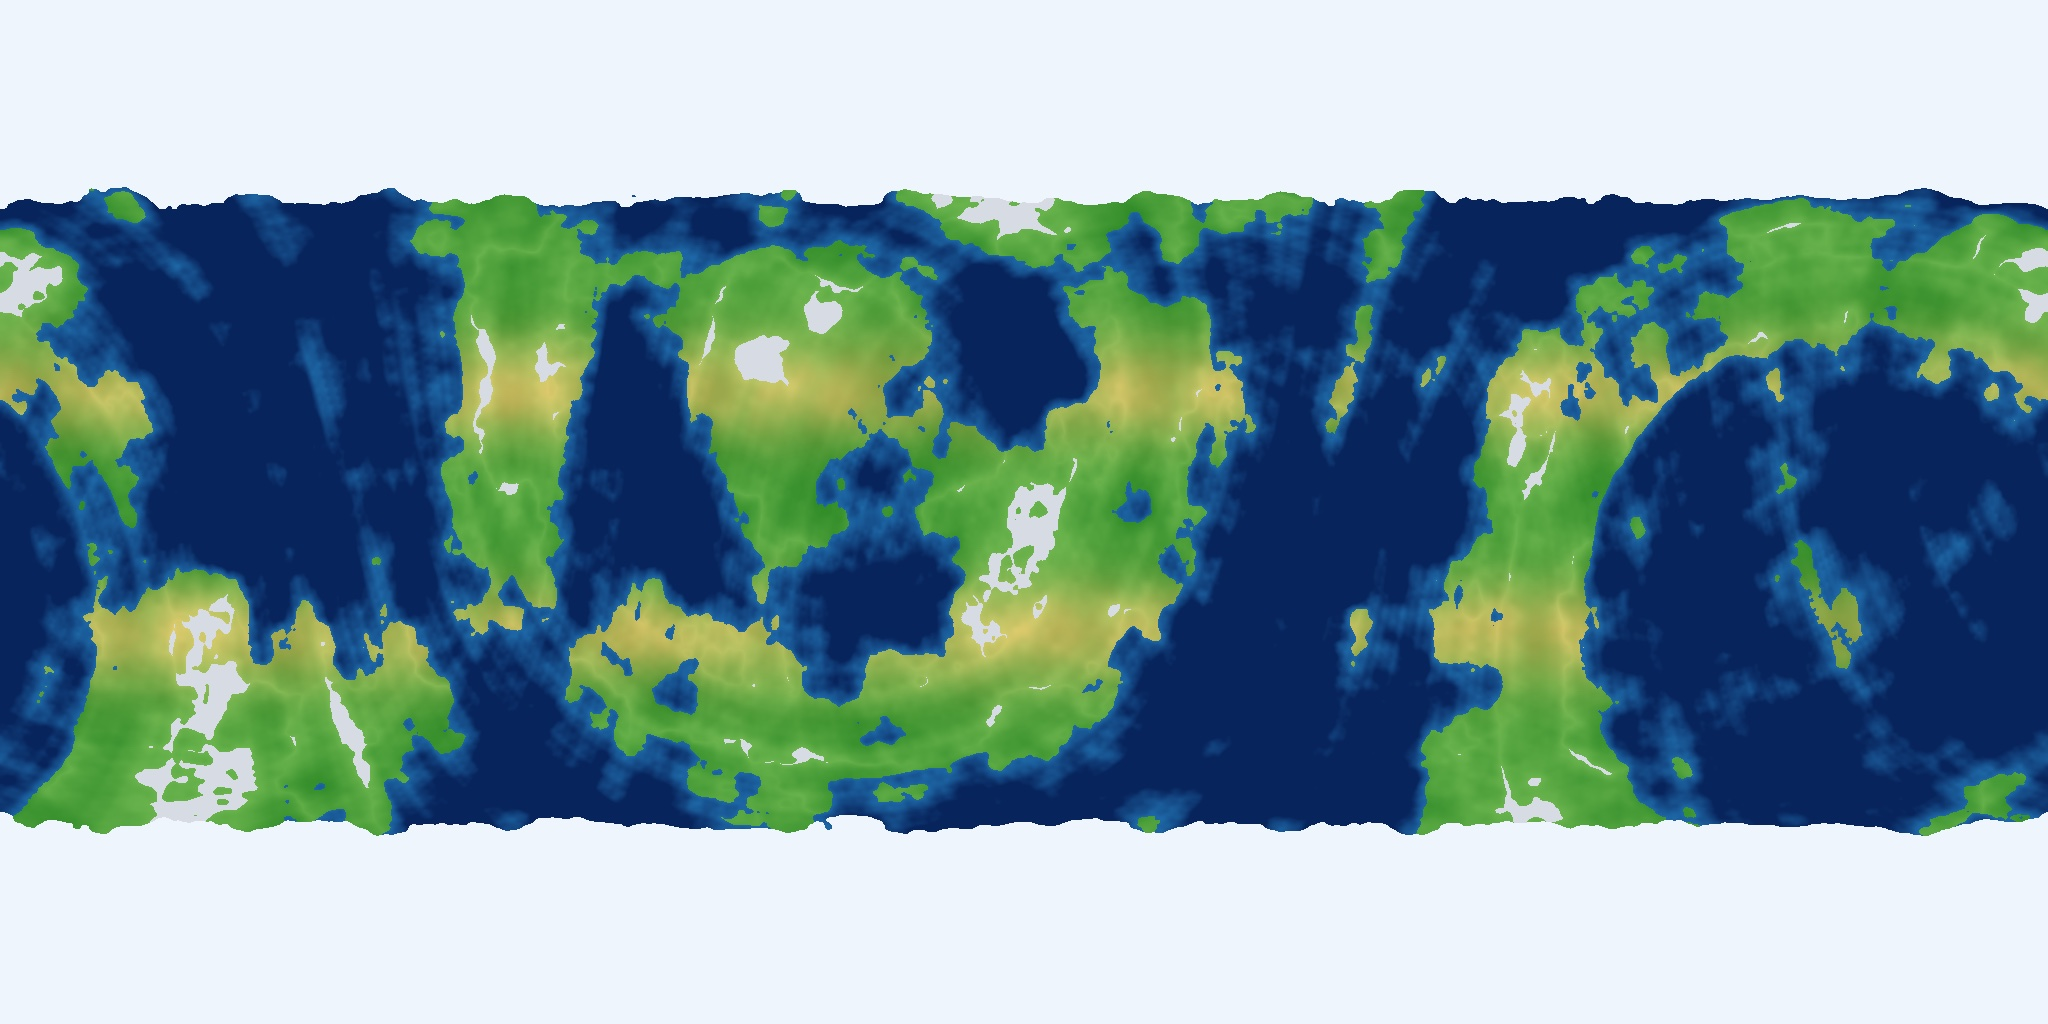
\includegraphics[width=\linewidth,height=4.4cm,keepaspectratio]{../public/textures/hd/earth_albedo.jpg}\\[2pt]
{\scriptsize\itshape\color{orbitarMuted} Planiglob desfășurat: Harta globală NASA Blue Marble a planetei Pământ, cu oceanele, continentele și calotele polare.}
\end{tabular}
\end{center}


\begin{tcolorbox}[orbitardata, title={\textbf{Repere esențiale: Pământul}}]
\small
\begin{itemize}[leftmargin=1.4em, itemsep=2pt, topsep=2pt]
  \item \textbf{Clasificare și orbită:} Planetă Telurică (Stâncoasă) \quad$\bullet$\quad \textbf{Distanță:} 1,000 UA ($\approx$ 150 milioane de kilometri)
  \item \textbf{Dimensiuni și masă:} rază medie 6.371 de kilometri \quad$\bullet$\quad masă: 1,000 $\times M_\oplus$
  \item \textbf{Gravitație și regim termic:} 1,000 $\times g_\oplus$ (9,81 m/s$^2$) \quad$\bullet$\quad temperatură medie: +15 $^\circ$C (înclinarea axei: 23,44$^\circ$)
  \item \textbf{Ciclu orbital și rotație:} perioadă orbitală (an): 365,256 zile ($\approx$ 1,00 ani pământești) \quad$\bullet$\quad rotație (zi): 23,93 ore (1,00 zile pământești)
  \item \textbf{Durata călătoriei de pe Pământ:} cu viteza luminii ($1c$): \emph{0,13 secunde în jurul Ecuatorului}; cu racheta ($50.000$ de kilometri pe oră): \emph{90 de minute pentru o orbită completă}; cu avionul ($900$ de kilometri pe oră): \emph{45 de ore în jurul lumii}; cu mașina ($100$ de kilometri pe oră): \emph{Ești deja aici! Înconjurul Ecuatorului durează 17 zile cu mașina}.
  \item \textbf{Repere de scară și curiozitate:} Văzut din spațiu, Pământul seamănă cu o bilă de sticlă albastră cu vârtejuri albe de frișcă! Pământul nu este perfect rotund: pentru că se învârte, este puțin turtit la poli ca o mandarină!
\end{itemize}
\end{tcolorbox}

\subsubsection*{Prezentare generală și profil astrofizic}
A treia planetă de la Soare definește distanța etalon de 1 Unitate Astronomică (149.597.870 de kilometri). Este singurul corp planetar cu tectonică a plăcilor activă, hidrosferă lichidă (71\% din suprafață) și atmosferă bogată în azot (78\%) și oxigen (21\%). Pământul este casa noastră minunată din cosmos! Are oceane albastre, continente verzi, nori albi și o pătură de aer respirabil care ne apără. Văzut din spațiu, Pământul seamănă cu o bilă de sticlă albastră cu vârtejuri albe de frișcă!

\subsubsection*{Alcătuirea fizică și structura internă}
Privind în profunzimea sa, alcătuirea fizică este organizată pe mai multe straturi și regiuni distincte, fiecare având un rol bine definit în evoluția și dinamica acestui obiect cosmic. În primul rând se remarcă \textbf{Nucleu intern solid și extern lichid}, aliaj de fier-nichel care generează magnetosfera protectoare împotriva radiațiilor cosmice. În strânsă legătură cu această componentă se află \textbf{Manta silicatată și Litosferă}, unde curenții de convecție din manta pun în mișcare plăcile tectonice ale scoarței. În completarea acestui ansamblu întâlnim \textbf{Hidrosferă și Atmosferă}, unde oceanele și straturile atmosferice (troposferă, stratosferă cu stratul de ozon) reglează clima.

\subsubsection*{Observații astronomice și istoricul explorării}
Observată continuu de flote de sateliți meteorologici și științifici (programul european Copernicus Sentinel, NASA EOS) și de echipajele de pe ISS. Pământul nu este perfect rotund: pentru că se învârte, este puțin turtit la poli ca o mandarină!

\vspace{6pt}
\begin{tcolorbox}[orbitarquiz, title={\textbf{Întrebare de verificare \#4: Pământul}}]
\textbf{Ce ne protejează planeta de particulele încărcate electric ale vântului solar?}
\begin{itemize}[leftmargin=2.2em, itemsep=2pt, topsep=4pt]
  \item[$\square$ \textbf{A.}] Câmpul magnetic (magnetosfera) generat de nucleul Pământului
  \item[$\square$ \textbf{B.}] Gravitația Lunii
  \item[$\square$ \textbf{C.}] Rotația în jurul Soarelui
  \item[$\square$ \textbf{D.}] Norii din troposferă
\end{itemize}
\vspace{2pt}
{\footnotesize\color{orbitarMuted}\textbf{Răspuns corect:} \textbf{A} (Câmpul magnetic (magnetosfera) generat de nucleul Pământului). \emph{Nucleul extern din fier lichid al Pământului funcționează ca un dinam și creează magnetosfera, care deviază vântul solar.}}
\end{tcolorbox}
\clearpage


\subsection{Luna}
\label{sec:body-moon}
\vspace{-4pt}
{\large\itshape\color{orbitarAccent} Singurul satelit natural al Pământului}\\[4pt]


\begin{center}
\begin{tabular}{@{}m{0.44\textwidth}@{\hspace{0.03\textwidth}}m{0.51\textwidth}@{}}
\centering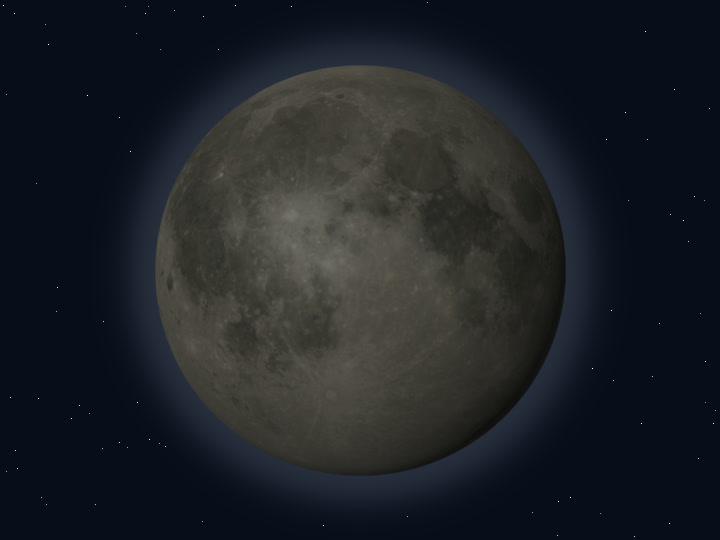
\includegraphics[width=\linewidth,height=4.4cm,keepaspectratio]{imagini/globuri/moon.jpg}\\[2pt]
{\scriptsize\itshape\color{orbitarMuted} Vedere 3D a corpului ceresc (\textbf{Luna})}
&
\centering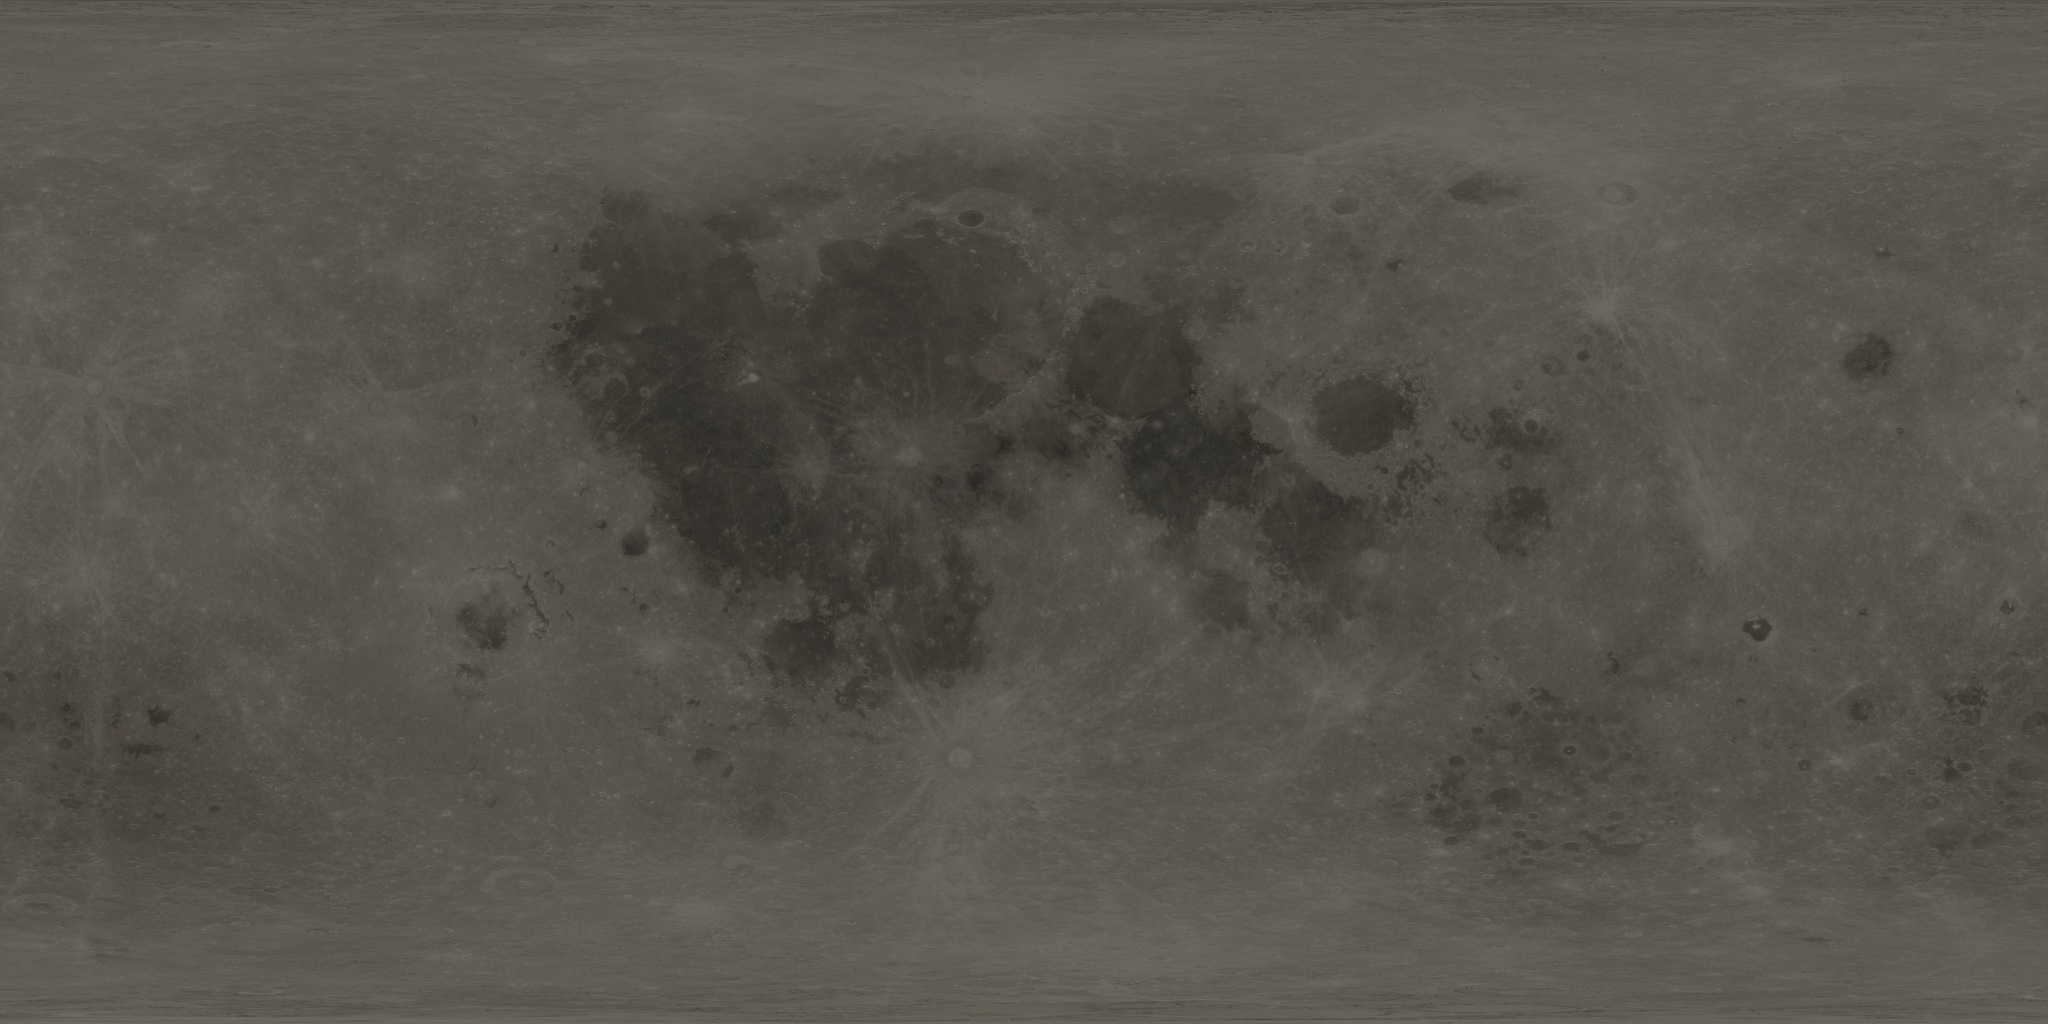
\includegraphics[width=\linewidth,height=4.4cm,keepaspectratio]{../public/textures/hd/moon_lro_albedo.jpg}\\[2pt]
{\scriptsize\itshape\color{orbitarMuted} Planiglob desfășurat: Harta globală a Lunii (NASA Lunar Reconnaissance Orbiter, LRO), cu mările bazaltice și craterele de impact.}
\end{tabular}
\end{center}


\begin{tcolorbox}[orbitardata, title={\textbf{Repere esențiale: Luna}}]
\small
\begin{itemize}[leftmargin=1.4em, itemsep=2pt, topsep=2pt]
  \item \textbf{Clasificare și orbită:} Satelit Natural (Lună) (orbitează în jurul: \textbf{Pământul}) \quad$\bullet$\quad \textbf{Distanță:} 1,000 UA ($\approx$ 150 milioane de kilometri)
  \item \textbf{Dimensiuni și masă:} rază medie 1.737,4 de kilometri \quad$\bullet$\quad masă: 0,012 $\times M_\oplus$
  \item \textbf{Gravitație și regim termic:} 0,165 $\times g_\oplus$ (1,62 m/s$^2$) \quad$\bullet$\quad temperatură medie: -23 $^\circ$C (înclinarea axei: 6,68$^\circ$)
  \item \textbf{Ciclu orbital și rotație:} perioadă orbitală (an): 27,322 zile pământești \quad$\bullet$\quad rotație (zi): 655,70 ore (27,32 zile pământești)
  \item \textbf{Durata călătoriei de pe Pământ:} cu viteza luminii ($1c$): \emph{1,28 secunde}; cu racheta ($50.000$ de kilometri pe oră): \emph{3 zile (misiunile Apollo)}; cu avionul ($900$ de kilometri pe oră): \emph{18 zile}; cu mașina ($100$ de kilometri pe oră): \emph{160 de zile (aproximativ 5 luni)}.
  \item \textbf{Repere de scară și curiozitate:} Dacă Pământul ar fi o minge de baschet, Luna ar fi cât o minge de tenis aflată la 7 metri distanță! Pe Lună gravitația este de 6 ori mai slabă decât pe Pământ: acolo ai putea sări de 6 ori mai sus!
\end{itemize}
\end{tcolorbox}

\subsubsection*{Prezentare generală și profil astrofizic}
Formată acum aproximativ 4,5 miliarde de ani în urma impactului dintre proto-Pământ și un corp de mărimea lui Marte (Theia), Luna se află în rotație sincronă (ne arată mereu aceeași față) și stabilizează înclinarea axei terestre. Luna este tovarășa fidelă a Pământului! Ea nu are lumină proprie, ci strălucește pe cerul nopții pentru că reflectă lumina Soarelui ca o oglindă. Dacă Pământul ar fi o minge de baschet, Luna ar fi cât o minge de tenis aflată la 7 metri distanță!

\subsubsection*{Alcătuirea fizică și structura internă}
Privind în profunzimea sa, alcătuirea fizică este organizată pe mai multe straturi și regiuni distincte, fiecare având un rol bine definit în evoluția și dinamica acestui obiect cosmic. În primul rând se remarcă \textbf{Nucleu mic de fier}, cu o rază de numai aproximativ 350 de kilometri, parțial topit la exterior. În strânsă legătură cu această componentă se află \textbf{Manta litosferică}, bogată în olivină și piroxen, mult mai rigidă decât mantaua Pământului. În completarea acestui ansamblu întâlnim \textbf{Scoarță acoperită cu regolit}, mări lunare întunecate (bazalt vulcanic antic) și podișuri înalte intens craterizate.

\subsubsection*{Observații astronomice și istoricul explorării}
Singurul corp ceresc pe care au pășit oamenii (12 astronauți în programul Apollo, 1969--1972) și ținta programului actual Artemis. Pe Lună gravitația este de 6 ori mai slabă decât pe Pământ: acolo ai putea sări de 6 ori mai sus!

\vspace{6pt}
\begin{tcolorbox}[orbitarquiz, title={\textbf{Întrebare de verificare \#5: Luna}}]
\textbf{De ce vedem de pe Pământ întotdeauna aceeași față a Lunii?}
\begin{itemize}[leftmargin=2.2em, itemsep=2pt, topsep=4pt]
  \item[$\square$ \textbf{A.}] Pentru că Luna nu se rotește deloc
  \item[$\square$ \textbf{B.}] Pentru că perioada de rotație a Lunii este egală cu perioada ei de orbitare în jurul Pământului
  \item[$\square$ \textbf{C.}] Pentru că cealaltă față este mereu în întuneric
  \item[$\square$ \textbf{D.}] Din cauza norilor terestri
\end{itemize}
\vspace{2pt}
{\footnotesize\color{orbitarMuted}\textbf{Răspuns corect:} \textbf{B} (Pentru că perioada de rotație a Lunii este egală cu perioada ei de orbitare în jurul Pământului). \emph{Fenomenul se numește rotație sincronă: Luna se rotește în jurul axei sale în exact 27,3 zile, adică în același timp în care înconjoară Pământul.}}
\end{tcolorbox}
\vspace{6pt}

\begin{tcolorbox}[orbitarcadet, title={\textbf{Repere Istorice pe Globul Lunii în Orbitar (\texttt{SurfaceMarkers.ts})}}]
Când te apropii cu camera 3D de \textbf{Lună} în aplicația \textbf{Orbitar}, pe suprafața ei se activează trei pini geografici interactivi care marchează locurile istorice unde astronauții programului \textbf{NASA Apollo} au pășit pe solul selenar:
\begin{itemize}[leftmargin=1.4em, itemsep=3pt]
  \item \textbf{Marea Liniștii (Apollo 11, $0{,}67^\circ\text{ N}, 23{,}47^\circ\text{ E}$, 20 iulie 1969):} locul istoric din \emph{Mare Tranquillitatis} unde modulul lunar «Eagle» pilotat de \textbf{Neil Armstrong} și \textbf{Buzz Aldrin} a aselenizat, iar oamenii au pășit pentru prima dată pe un alt corp ceresc: \emph{„Un pas mic pentru om, un salt uriaș pentru omenire!”}
  \item \textbf{Mons Hadley (Apollo 15, $26{,}13^\circ\text{ N}, 3{,}63^\circ\text{ E}$, 30 iulie 1971):} situat în Munții Apenini Lunari, lângă canalul vulcanic \emph{Hadley Rille}; prima misiune în care astronauții \textbf{David Scott} și \textbf{James Irwin} au condus automobilul electric \emph{Lunar Roving Vehicle (LRV)} și au descoperit faimoasa «Piatră a Genezei».
  \item \textbf{Valea Taurus-Littrow (Apollo 17, $20{,}19^\circ\text{ N}, 30{,}77^\circ\text{ E}$, 11 decembrie 1972):} cea mai recentă aselenizare cu echipaj uman (\textbf{Eugene Cernan} și geologul \textbf{Harrison Schmitt}), care a condus la descoperirea solului portocaliu din micro-sfere de sticlă vulcanică lunară.
\end{itemize}
\end{tcolorbox}

\clearpage


\section{Marte}
\label{sec:body-mars}
\vspace{-4pt}
{\large\itshape\color{orbitarAccent} Planeta Roșie a vulcanilor giganți și a roverelor exploratoare}\\[4pt]


\begin{center}
\begin{tabular}{@{}m{0.44\textwidth}@{\hspace{0.03\textwidth}}m{0.51\textwidth}@{}}
\centering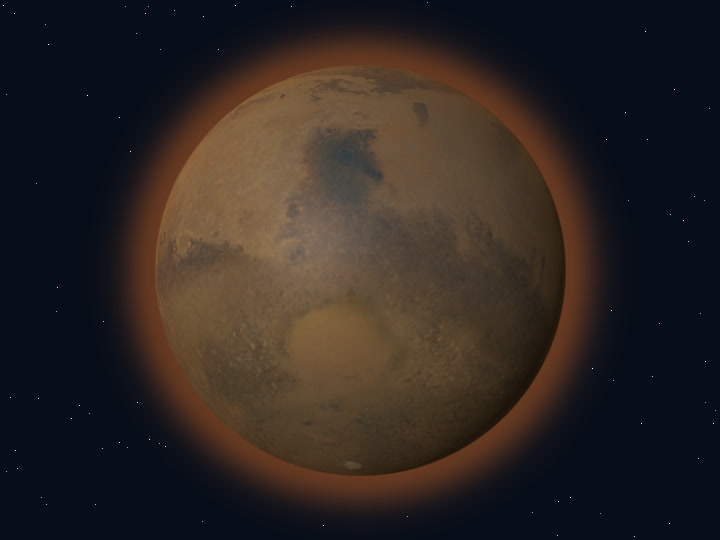
\includegraphics[width=\linewidth,height=4.4cm,keepaspectratio]{imagini/globuri/mars.jpg}\\[2pt]
{\scriptsize\itshape\color{orbitarMuted} Vedere 3D a corpului ceresc (\textbf{Marte})}
&
\centering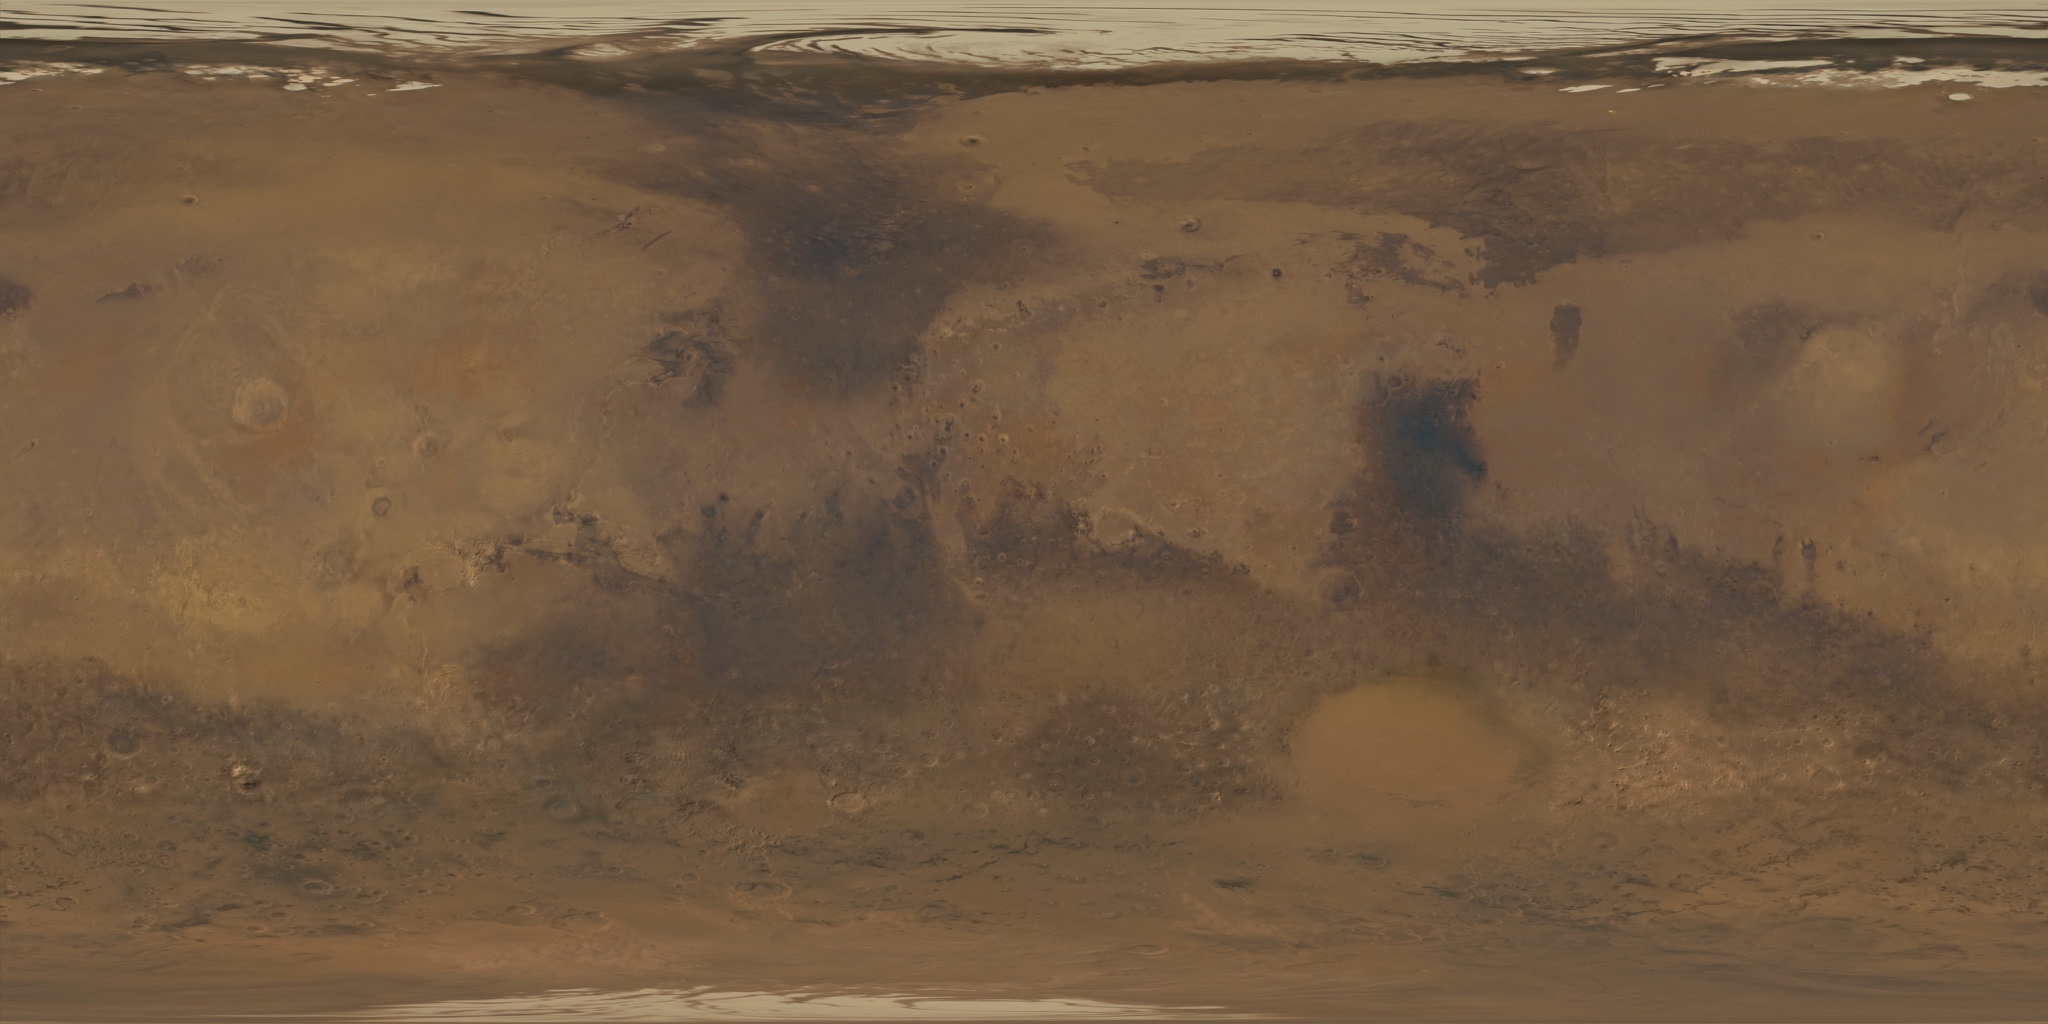
\includegraphics[width=\linewidth,height=4.4cm,keepaspectratio]{../public/textures/hd/mars_viking_albedo.jpg}\\[2pt]
{\scriptsize\itshape\color{orbitarMuted} Planiglob desfășurat: Harta globală a Planetei Roșii Marte (mozaic NASA Viking / MOLA), evidențiind Valles Marineris și regiunea vulcanică Tharsis.}
\end{tabular}
\end{center}


\begin{tcolorbox}[orbitardata, title={\textbf{Repere esențiale: Marte}}]
\small
\begin{itemize}[leftmargin=1.4em, itemsep=2pt, topsep=2pt]
  \item \textbf{Clasificare și orbită:} Planetă Telurică (Stâncoasă) \quad$\bullet$\quad \textbf{Distanță:} 1,524 UA ($\approx$ 228 milioane de kilometri)
  \item \textbf{Dimensiuni și masă:} rază medie 3.389,5 de kilometri \quad$\bullet$\quad masă: 0,107 $\times M_\oplus$
  \item \textbf{Gravitație și regim termic:} 0,380 $\times g_\oplus$ (3,73 m/s$^2$) \quad$\bullet$\quad temperatură medie: -63 $^\circ$C (înclinarea axei: 25,19$^\circ$)
  \item \textbf{Ciclu orbital și rotație:} perioadă orbitală (an): 686,98 zile ($\approx$ 1,88 ani pământești) \quad$\bullet$\quad rotație (zi): 24,62 ore (1,03 zile pământești)
  \item \textbf{Durata călătoriei de pe Pământ:} cu viteza luminii ($1c$): \emph{între 3 și 22 de minute}; cu racheta ($50.000$ de kilometri pe oră): \emph{7 luni}; cu avionul ($900$ de kilometri pe oră): \emph{7 ani}; cu mașina ($100$ de kilometri pe oră): \emph{62 de ani (la apropierea minimă)}.
  \item \textbf{Repere de scară și curiozitate:} Marte este cam pe jumătate cât Pământul: dacă Pământul ar fi o portocală, Marte ar fi o caisă roșiatică! Pe Marte se află Olympus Mons, un vulcan stins de trei ori mai înalt decât vârful Everest!
\end{itemize}
\end{tcolorbox}

\subsubsection*{Prezentare generală și profil astrofizic}
A patra planetă de la Soare are o zi solară (numită \guillemotleft{}sol\guillemotright{}) de 24 de ore și 39 de minute, foarte apropiată de cea terestră. Văile râurilor secate și mineralele hidratate demonstrează că Marte a avut oceane de apă lichidă acum peste 3,5 miliarde de ani. Marte este numită Planeta Roșie deoarece solul ei este plin de praf de fier ruginit! Este singura planetă locuită exclusiv de roboți și rovere trimise de oameni. Marte este cam pe jumătate cât Pământul: dacă Pământul ar fi o portocală, Marte ar fi o caisă roșiatică!

\subsubsection*{Alcătuirea fizică și structura internă}
Privind în profunzimea sa, alcătuirea fizică este organizată pe mai multe straturi și regiuni distincte, fiecare având un rol bine definit în evoluția și dinamica acestui obiect cosmic. În primul rând se remarcă \textbf{Nucleu metalic}, compus din fier, nichel și sulf (aproximativ 1.830 de kilometri rază), măsurat cu precizie de sonda InSight. În strânsă legătură cu această componentă se află \textbf{Scoarță bazaltică bogată în oxid de fier}, care găzduiește canionul Valles Marineris (4.000 de kilometri lungime) și calote polare din gheață și CO$_2$ solid. În completarea acestui ansamblu întâlnim \textbf{Atmosferă rarefiată (0,6\% din presiunea terestră)}, alcătuită în proporție de 95\% dioxid de carbon, capabilă totuși să susțină furtuni globale de praf.

\subsubsection*{Observații astronomice și istoricul explorării}
Explorată de sondele Viking, Mars Reconnaissance Orbiter, MAVEN și roverele Sojourner, Spirit, Opportunity, Curiosity și Perseverance. Pe Marte se află Olympus Mons, un vulcan stins de trei ori mai înalt decât vârful Everest!

\vspace{6pt}
\begin{tcolorbox}[orbitarquiz, title={\textbf{Întrebare de verificare \#6: Marte}}]
\textbf{Cum se numește cel mai înalt vulcan de pe Marte și din întregul Sistem Solar?}
\begin{itemize}[leftmargin=2.2em, itemsep=2pt, topsep=4pt]
  \item[$\square$ \textbf{A.}] Mauna Kea
  \item[$\square$ \textbf{B.}] Olympus Mons
  \item[$\square$ \textbf{C.}] Valles Marineris
  \item[$\square$ \textbf{D.}] Maxwell Montes
\end{itemize}
\vspace{2pt}
{\footnotesize\color{orbitarMuted}\textbf{Răspuns corect:} \textbf{B} (Olympus Mons). \emph{Olympus Mons are o altitudine de aproape 22 de kilometri și o bază de aproximativ 600 de kilometri diametru!}}
\end{tcolorbox}
\clearpage


\subsection{Phobos}
\label{sec:body-phobos}
\vspace{-4pt}
{\large\itshape\color{orbitarAccent} Luna interioară în formă de cartof a planetei Marte}\\[4pt]


\begin{center}
\begin{tabular}{@{}m{0.44\textwidth}@{\hspace{0.03\textwidth}}m{0.51\textwidth}@{}}
\centering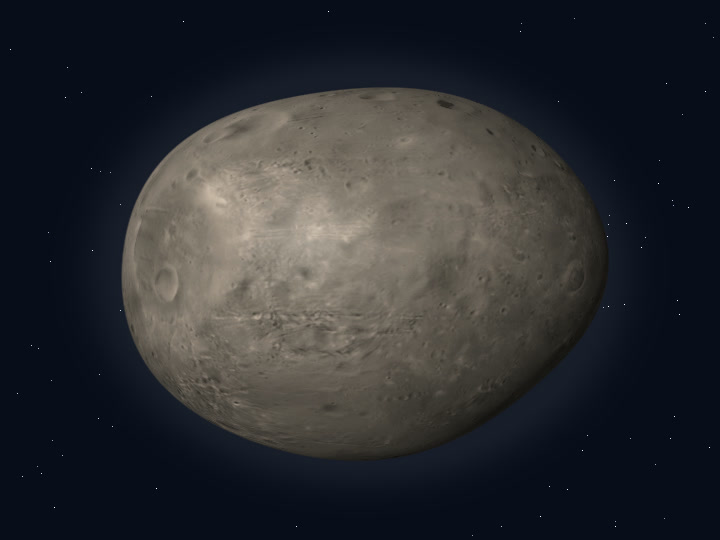
\includegraphics[width=\linewidth,height=4.4cm,keepaspectratio]{imagini/globuri/phobos.jpg}\\[2pt]
{\scriptsize\itshape\color{orbitarMuted} Vedere 3D a corpului ceresc (\textbf{Phobos})}
&
\centering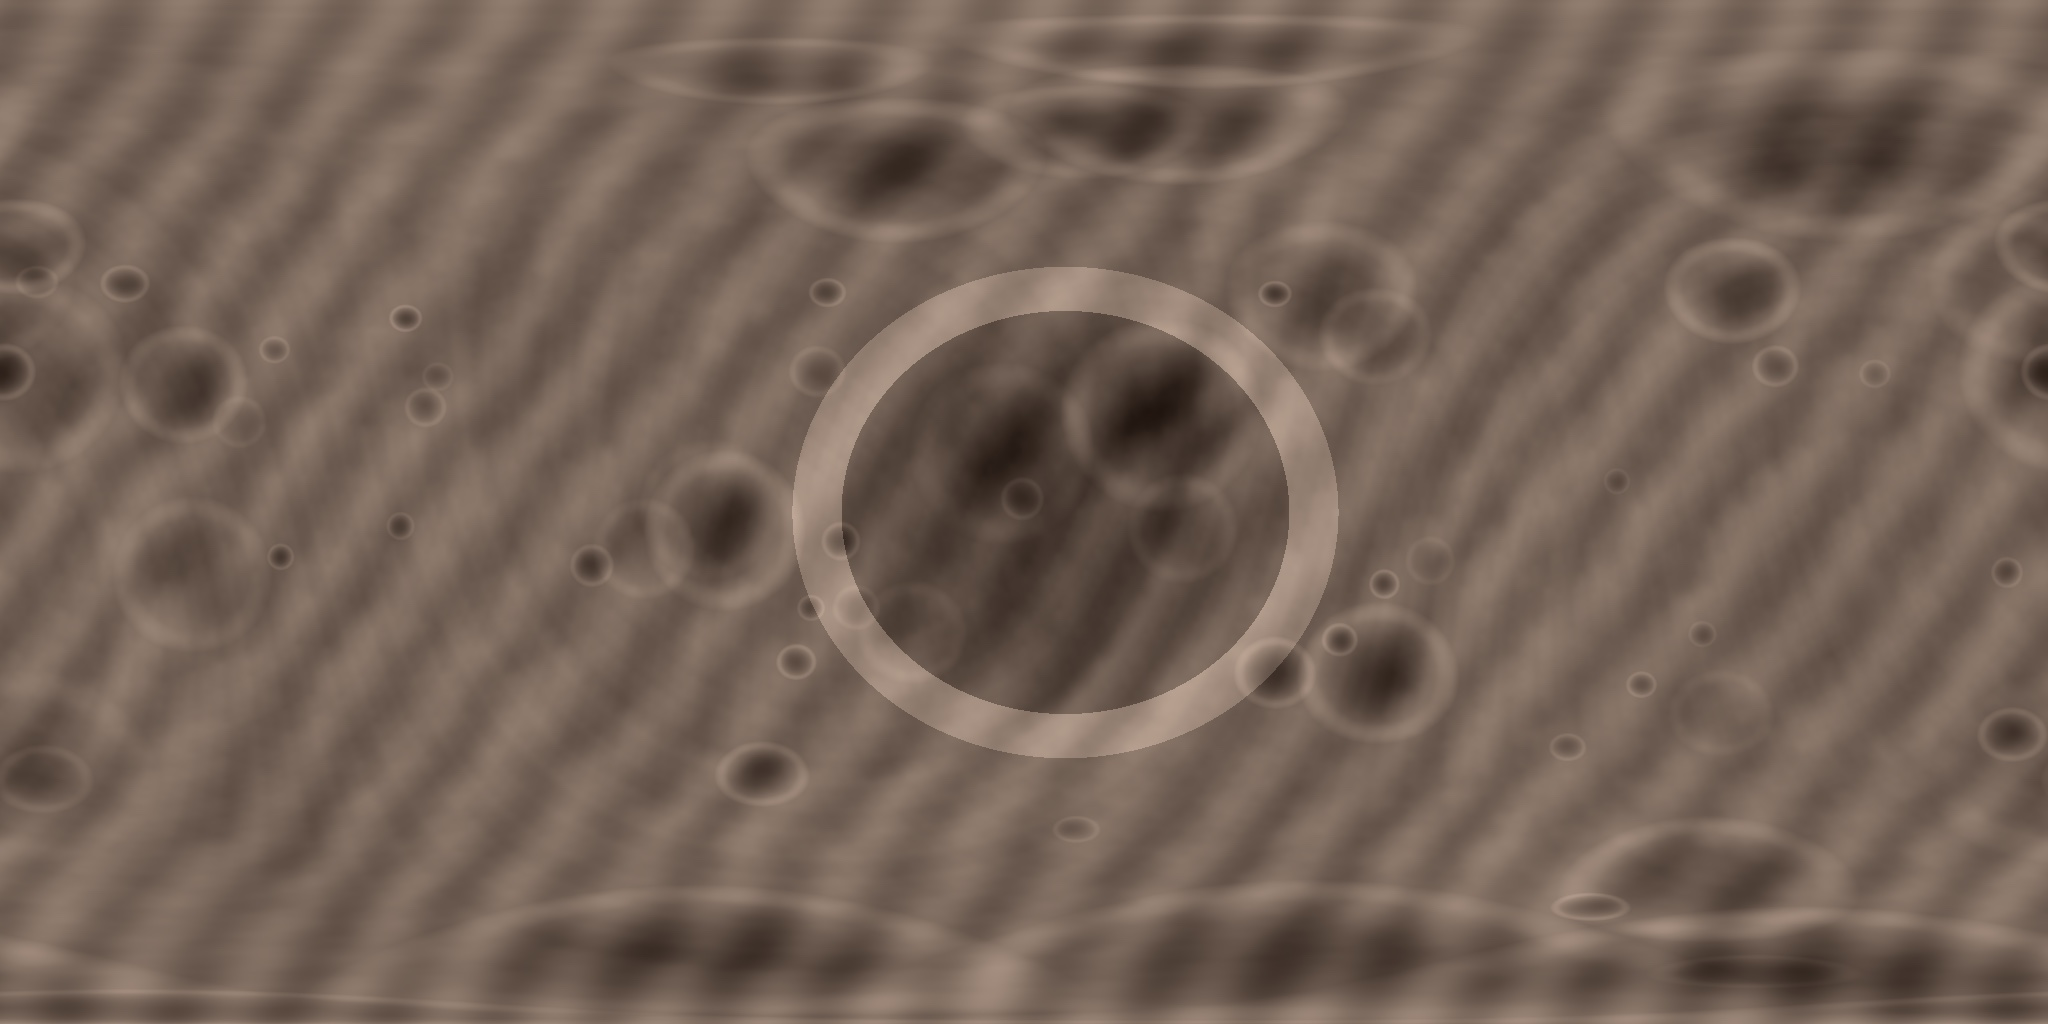
\includegraphics[width=\linewidth,height=4.4cm,keepaspectratio]{../public/textures/hd/phobos_viking.jpg}\\[2pt]
{\scriptsize\itshape\color{orbitarMuted} Planiglob desfășurat: Harta suprafeței satelitul marțian Phobos și a marelui crater Stickney (date NASA Viking).}
\end{tabular}
\end{center}


\begin{tcolorbox}[orbitardata, title={\textbf{Repere esențiale: Phobos}}]
\small
\begin{itemize}[leftmargin=1.4em, itemsep=2pt, topsep=2pt]
  \item \textbf{Clasificare și orbită:} Satelit Natural (Lună) (orbitează în jurul: \textbf{Marte}) \quad$\bullet$\quad \textbf{Distanță:} 1,524 UA ($\approx$ 228 milioane de kilometri)
  \item \textbf{Dimensiuni și masă:} rază medie 11,27 kilometri \quad$\bullet$\quad masă: 1,80e-9 $\times M_\oplus$
  \item \textbf{Gravitație și regim termic:} 0,001 $\times g_\oplus$ (0,01 m/s$^2$) \quad$\bullet$\quad temperatură medie: -40 $^\circ$C (înclinarea axei: Nespecificată)
  \item \textbf{Ciclu orbital și rotație:} perioadă orbitală (an): 0,319 zile pământești \quad$\bullet$\quad rotație (zi): 7,65 ore (0,32 zile pământești)
  \item \textbf{Durata călătoriei de pe Pământ:} cu viteza luminii ($1c$): \emph{între 3 și 22 de minute}; cu racheta ($50.000$ de kilometri pe oră): \emph{7 luni}; cu avionul ($900$ de kilometri pe oră): \emph{7 ani}; cu mașina ($100$ de kilometri pe oră): \emph{62 de ani}.
  \item \textbf{Repere de scară și curiozitate:} Phobos zboară atât de aproape și de repede deasupra lui Marte încât răsare și apune de două ori într-o singură zi marțiană! Pe Phobos se află Craterul Stickney, o urmă de impact atât de uriașă încât aproape a spart mica lună în bucăți!
\end{itemize}
\end{tcolorbox}

\subsubsection*{Prezentare generală și profil astrofizic}
Descoperită în 1877 de astronomul Asaph Hall, Phobos orbitează la numai 6.000 de kilometri deasupra suprafeței marțiene, fiind mai aproape de planeta sa decât orice alt satelit natural din Sistemul Solar. Perioada sa orbitală de 7 ore și 39 de minute este de trei ori mai scurtă decât rotația lui Marte. Phobos este cea mai mare dintre cele două luni ale lui Marte! Nu este rotundă ca Luna noastră, ci are forma unui cartof stâncos plin de cratere și șanțuri. Phobos zboară atât de aproape și de repede deasupra lui Marte încât răsare și apune de două ori într-o singură zi marțiană!

\subsubsection*{Alcătuirea fizică și structura internă}
Privind în profunzimea sa, alcătuirea fizică este organizată pe mai multe straturi și regiuni distincte, fiecare având un rol bine definit în evoluția și dinamica acestui obiect cosmic. În primul rând se remarcă \textbf{Interior poros tip \guillemotleft{}rubble-pile\guillemotright{}}, compus din blocuri de rocă condritică și goluri interne (30\% porozitate), probabil un asteroid capturat. În strânsă legătură cu această componentă se află \textbf{Craterul gigant Stickney (9 kilometri diametru)}, care ocupă aproape jumătate din fața vizibilă a satelitului și este înconjurat de șanțuri paralele de stres. În completarea acestui ansamblu întâlnim \textbf{Strat gros de regolit}, praf fin de până la 100 de metri adâncime, creat de miliarde de ani de bombardament meteoritic.

\subsubsection*{Observații astronomice și istoricul explorării}
Fotografiată de aproape de sondele Mariner 9, Viking 1, Mars Global Surveyor, Mars Express și Mars Reconnaissance Orbiter; ținta viitoarei misiuni japoneze MMX (Martian Moons eXploration). Pe Phobos se află Craterul Stickney, o urmă de impact atât de uriașă încât aproape a spart mica lună în bucăți!

\vspace{6pt}
\begin{tcolorbox}[orbitarquiz, title={\textbf{Întrebare de verificare \#7: Phobos}}]
\textbf{De ce răsare Phobos din vest și apune în est pe cerul planetei Marte?}
\begin{itemize}[leftmargin=2.2em, itemsep=2pt, topsep=4pt]
  \item[$\square$ \textbf{A.}] Pentru că se rotește în jurul lui Marte în 7 ore și 39 de minute, mai repede decât se învârte Marte în jurul axei sale
  \item[$\square$ \textbf{B.}] Pentru că Marte stă pe loc
  \item[$\square$ \textbf{C.}] Din cauza furtunilor de nisip
  \item[$\square$ \textbf{D.}] Pentru că orbitează direct Soarele
\end{itemize}
\vspace{2pt}
{\footnotesize\color{orbitarMuted}\textbf{Răspuns corect:} \textbf{A} (Pentru că se rotește în jurul lui Marte în 7 ore și 39 de minute, mai repede decât se învârte Marte în jurul axei sale). \emph{Phobos înconjoară Marte în doar 7,65 ore, în timp ce o zi pe Marte durează 24,6 ore, deci satelitul depășește rotația planetei.}}
\end{tcolorbox}
\clearpage


\subsection{Deimos}
\label{sec:body-deimos}
\vspace{-4pt}
{\large\itshape\color{orbitarAccent} Luna exterioară, mică și netedă, a planetei Marte}\\[4pt]


\begin{center}
\begin{tabular}{@{}m{0.44\textwidth}@{\hspace{0.03\textwidth}}m{0.51\textwidth}@{}}
\centering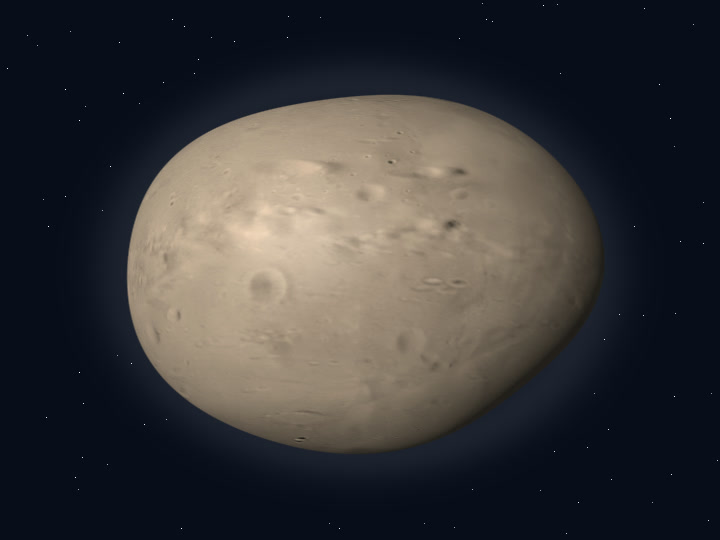
\includegraphics[width=\linewidth,height=4.4cm,keepaspectratio]{imagini/globuri/deimos.jpg}\\[2pt]
{\scriptsize\itshape\color{orbitarMuted} Vedere 3D a corpului ceresc (\textbf{Deimos})}
&
\centering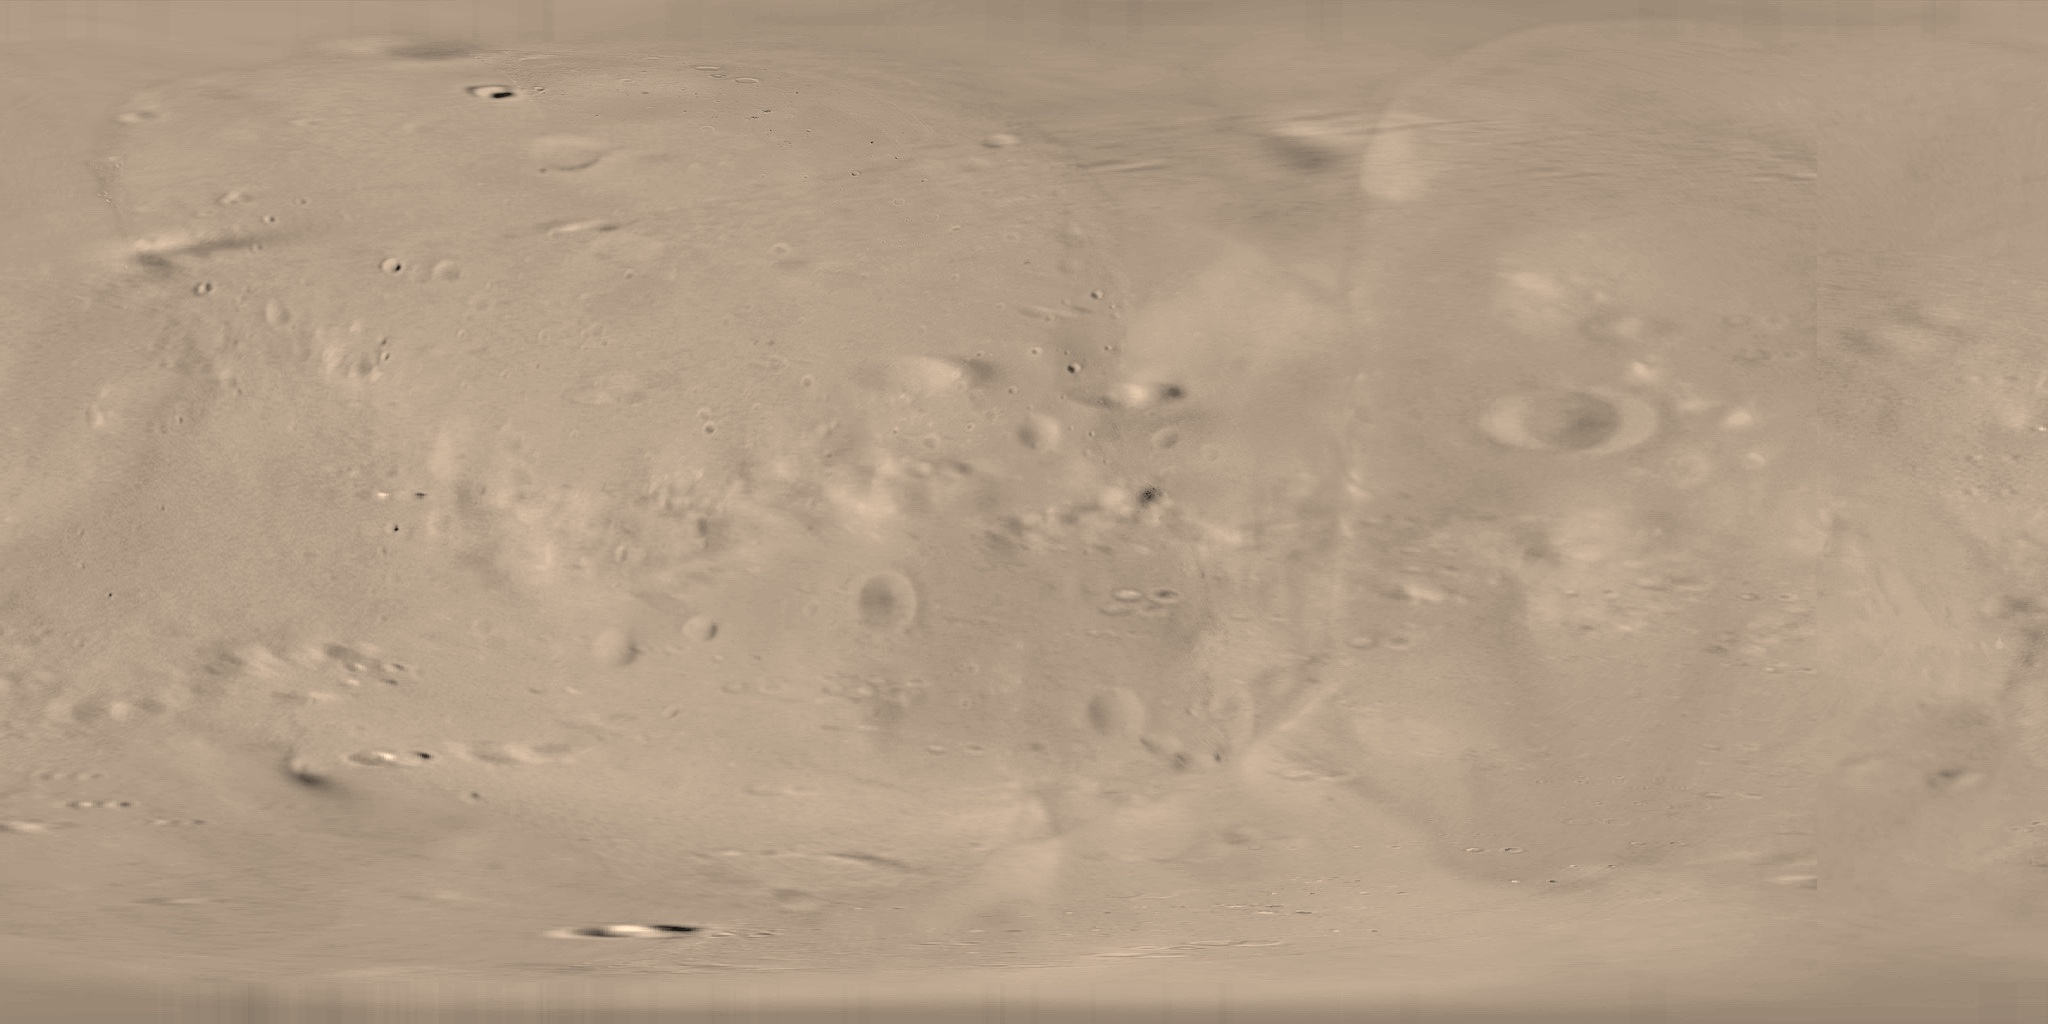
\includegraphics[width=\linewidth,height=4.4cm,keepaspectratio]{../public/textures/hd/deimos_viking.jpg}\\[2pt]
{\scriptsize\itshape\color{orbitarMuted} Planiglob desfășurat: Harta suprafeței netede și prăfuite a lui Deimos, satelitul exterior al lui Marte (date NASA Viking).}
\end{tabular}
\end{center}


\begin{tcolorbox}[orbitardata, title={\textbf{Repere esențiale: Deimos}}]
\small
\begin{itemize}[leftmargin=1.4em, itemsep=2pt, topsep=2pt]
  \item \textbf{Clasificare și orbită:} Satelit Natural (Lună) (orbitează în jurul: \textbf{Marte}) \quad$\bullet$\quad \textbf{Distanță:} 1,524 UA ($\approx$ 228 milioane de kilometri)
  \item \textbf{Dimensiuni și masă:} rază medie 6,2 kilometri \quad$\bullet$\quad masă: 2,50e-10 $\times M_\oplus$
  \item \textbf{Gravitație și regim termic:} Microgravitație / Imponderabilitate ($\approx 0\,g$) \quad$\bullet$\quad temperatură medie: -40 $^\circ$C (înclinarea axei: Nespecificată)
  \item \textbf{Ciclu orbital și rotație:} perioadă orbitală (an): 1,263 zile pământești \quad$\bullet$\quad rotație (zi): 30,31 ore (1,26 zile pământești)
  \item \textbf{Durata călătoriei de pe Pământ:} cu viteza luminii ($1c$): \emph{între 3 și 22 de minute}; cu racheta ($50.000$ de kilometri pe oră): \emph{7 luni}; cu avionul ($900$ de kilometri pe oră): \emph{7 ani}; cu mașina ($100$ de kilometri pe oră): \emph{62 de ani}.
  \item \textbf{Repere de scară și curiozitate:} Gravitația pe Deimos este atât de mică încât, dacă ai alerga repede și ai sări, te-ai desprinde de sol și ai pluti direct în spațiu! Văzut de pe suprafața lui Marte, Deimos pare doar o stea foarte strălucitoare, puțin mai mare decât planeta Venus!
\end{itemize}
\end{tcolorbox}

\subsubsection*{Prezentare generală și profil astrofizic}
Descoperită tot de Asaph Hall în august 1877, Deimos orbitează la 23.460 de kilometri de centrul lui Marte în 30,3 ore. Cu o rază medie de doar 6,2 kilometri, este unul dintre cei mai mici sateliți cunoscuți din Sistemul Solar. Deimos este fratele mai mic al lui Phobos și a doua lună a lui Marte! Este o stâncă mică, acoperită cu o pătură groasă de praf fin care îi netezește craterele. Gravitația pe Deimos este atât de mică încât, dacă ai alerga repede și ai sări, te-ai desprinde de sol și ai pluti direct în spațiu!

\subsubsection*{Alcătuirea fizică și structura internă}
Privind în profunzimea sa, alcătuirea fizică este organizată pe mai multe straturi și regiuni distincte, fiecare având un rol bine definit în evoluția și dinamica acestui obiect cosmic. În primul rând se remarcă \textbf{Corp condritic bogat în carbon}, densitate scăzută de 1,47 g/cm$^3$, similară asteroizilor de tip C și D din centura exterioară. În strânsă legătură cu această componentă se află \textbf{Craterele Swift și Voltaire}, cele două cratere principale (de aproximativ 1--3 kilometri lărgime), numite după scriitorii care au imaginat două luni marțiene înainte de descoperirea lor. În completarea acestui ansamblu întâlnim \textbf{Manta netedă de regolit}, unde craterele sunt parțial umplute cu praf marțian-asteroidal, oferind un relief mult mai blând decât cel de pe Phobos.

\subsubsection*{Observații astronomice și istoricul explorării}
Fotografiată în detaliu de sonda Viking 2 în 1977 (de la numai 30 de kilometri distanță), de Mars Reconnaissance Orbiter și în 2023 de sonda Emiratelor Arabe Unite \guillemotleft{}Hope\guillemotright{} (Al-Amal). Văzut de pe suprafața lui Marte, Deimos pare doar o stea foarte strălucitoare, puțin mai mare decât planeta Venus!

\vspace{6pt}
\begin{tcolorbox}[orbitarquiz, title={\textbf{Întrebare de verificare \#8: Deimos}}]
\textbf{Cum arată suprafața satelitului Deimos în comparație cu cea a lui Phobos?}
\begin{itemize}[leftmargin=2.2em, itemsep=2pt, topsep=4pt]
  \item[$\square$ \textbf{A.}] Este acoperită cu gheață albastră
  \item[$\square$ \textbf{B.}] Este mult mai netedă, deoarece craterele sunt umplute cu un strat gros de praf (regolit)
  \item[$\square$ \textbf{C.}] Are vulcani activi
  \item[$\square$ \textbf{D.}] Este perfect rotundă ca o bilă de oțel
\end{itemize}
\vspace{2pt}
{\footnotesize\color{orbitarMuted}\textbf{Răspuns corect:} \textbf{B} (Este mult mai netedă, deoarece craterele sunt umplute cu un strat gros de praf (regolit)). \emph{Deimos este acoperit cu un strat gros de regolit pulverulent care a umplut craterele vechi, dându-i un aspect catifelat.}}
\end{tcolorbox}
\clearpage


\section{Jupiter}
\label{sec:body-jupiter}
\vspace{-4pt}
{\large\itshape\color{orbitarAccent} Cel mai masiv gigant gazos din Sistemul Solar}\\[4pt]


\begin{center}
\begin{tabular}{@{}m{0.44\textwidth}@{\hspace{0.03\textwidth}}m{0.51\textwidth}@{}}
\centering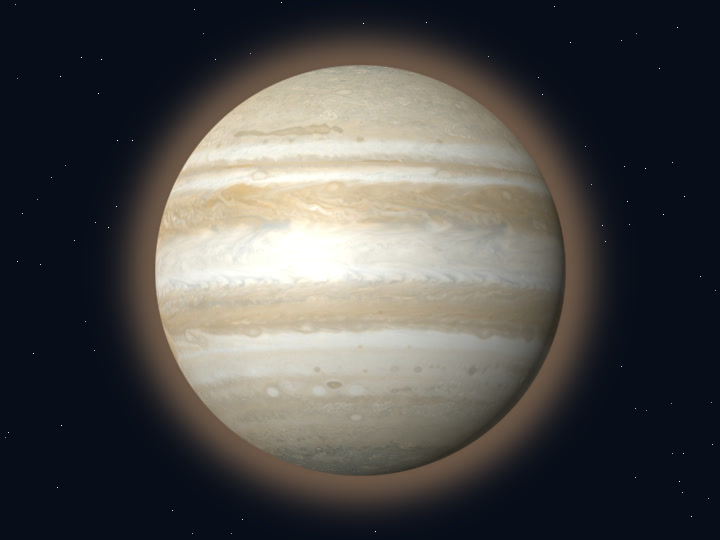
\includegraphics[width=\linewidth,height=4.4cm,keepaspectratio]{imagini/globuri/jupiter.jpg}\\[2pt]
{\scriptsize\itshape\color{orbitarMuted} Vedere 3D a corpului ceresc (\textbf{Jupiter})}
&
\centering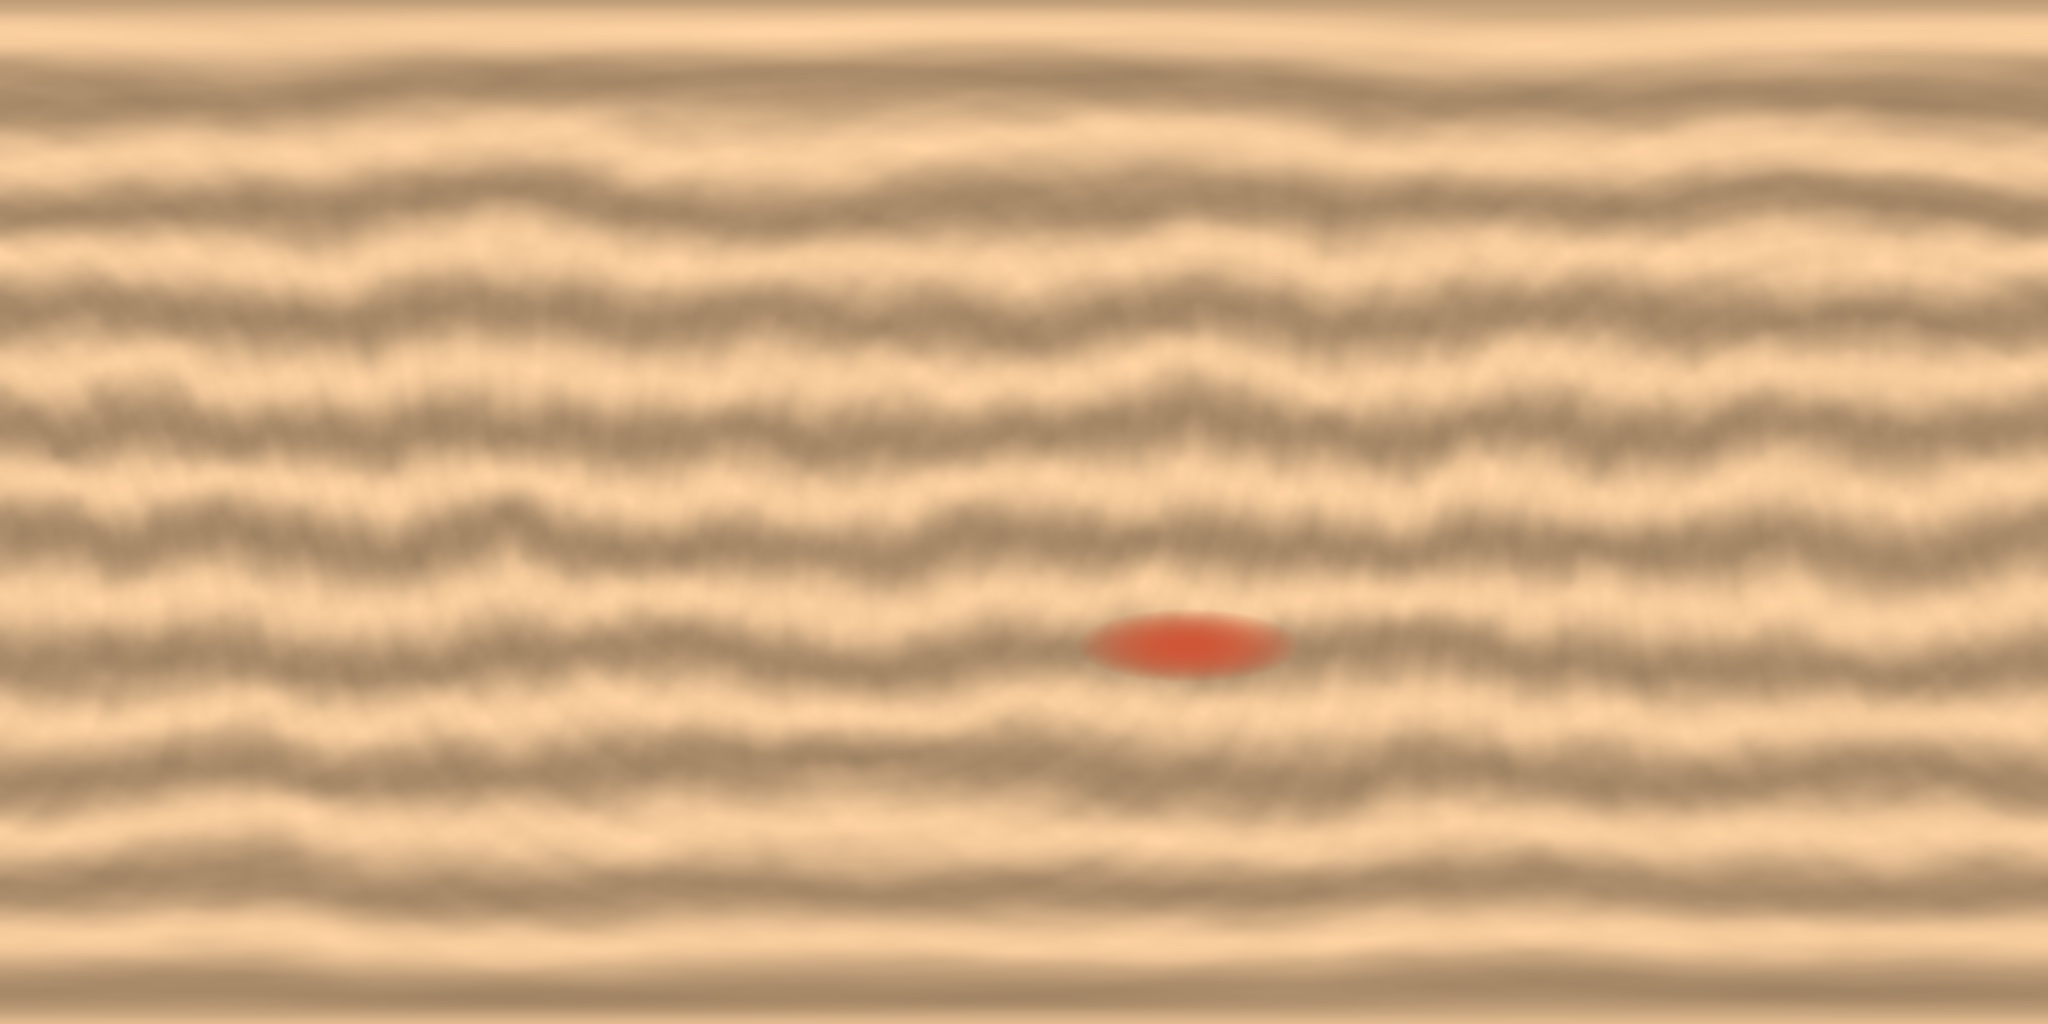
\includegraphics[width=\linewidth,height=4.4cm,keepaspectratio]{../public/textures/hd/jupiter_cassini_albedo.jpg}\\[2pt]
{\scriptsize\itshape\color{orbitarMuted} Planiglob desfășurat: Harta globală a benzilor de nori și a Marii Pete Roșii de pe Jupiter, fotografiată de sonda NASA/ESA Cassini.}
\end{tabular}
\end{center}


\begin{tcolorbox}[orbitardata, title={\textbf{Repere esențiale: Jupiter}}]
\small
\begin{itemize}[leftmargin=1.4em, itemsep=2pt, topsep=2pt]
  \item \textbf{Clasificare și orbită:} Gigant Gazos \quad$\bullet$\quad \textbf{Distanță:} 5,204 UA ($\approx$ 779 milioane de kilometri)
  \item \textbf{Dimensiuni și masă:} rază medie 69.911 kilometri \quad$\bullet$\quad masă: 317,800 $\times M_\oplus$
  \item \textbf{Gravitație și regim termic:} 2,530 $\times g_\oplus$ (24,82 m/s$^2$) \quad$\bullet$\quad temperatură medie: -110 $^\circ$C (înclinarea axei: 3,13$^\circ$)
  \item \textbf{Ciclu orbital și rotație:} perioadă orbitală (an): 4.332,59 zile ($\approx$ 11,86 ani pământești) \quad$\bullet$\quad rotație (zi): 9,93 ore (0,41 zile pământești)
  \item \textbf{Durata călătoriei de pe Pământ:} cu viteza luminii ($1c$): \emph{35 de minute}; cu racheta ($50.000$ de kilometri pe oră): \emph{2 până la 5 ani}; cu avionul ($900$ de kilometri pe oră): \emph{80 de ani}; cu mașina ($100$ de kilometri pe oră): \emph{717 ani}.
  \item \textbf{Repere de scară și curiozitate:} Dacă Pământul ar fi un bob de strugure, Jupiter ar fi cât un pepene verde imens! Marea Pată Roșie de pe Jupiter este o furtună gigantică ce suflă de sute de ani și e mai mare decât tot Pământul!
\end{itemize}
\end{tcolorbox}

\subsubsection*{Prezentare generală și profil astrofizic}
Jupiter are o masă de 2,5 ori mai mare decât a tuturor celorlalte planete la un loc. Se rotește în jurul axei sale în mai puțin de 10 ore, ceea ce creează benzi atmosferice spectaculoase (zone și centuri) și cel mai puternic câmp magnetic planetar. Jupiter este uriașul protector al Sistemului Solar! Nu are un sol tare pe care să poți păși, fiind alcătuit aproape în întregime din nori și gaze. Dacă Pământul ar fi un bob de strugure, Jupiter ar fi cât un pepene verde imens!

\subsubsection*{Alcătuirea fizică și structura internă}
Privind în profunzimea sa, alcătuirea fizică este organizată pe mai multe straturi și regiuni distincte, fiecare având un rol bine definit în evoluția și dinamica acestui obiect cosmic. În primul rând se remarcă \textbf{Nucleu difuz stâncos și de gheață}, un nucleu central de mare presiune amestecat cu hidrogen metalic. În strânsă legătură cu această componentă se află \textbf{Ocean de hidrogen metalic lichid}, unde la presiuni de milioane de atmosfere, hidrogenul devine conductor electric și generează magnetosfera uriașă. În completarea acestui ansamblu întâlnim \textbf{Atmosferă de hidrogen (90\%) și heliu (10\%)}, nori de amoniac și hidrosulfură de amoniu organizați în jeturi zonale și anticicloane.

\subsubsection*{Observații astronomice și istoricul explorării}
Survolată de Pioneer 10/11, Voyager 1/2, Ulysses, Cassini și New Horizons; studiată pe orbită de sondele Galileo (1995--2003) și Juno (din 2016). Marea Pată Roșie de pe Jupiter este o furtună gigantică ce suflă de sute de ani și e mai mare decât tot Pământul!

\vspace{6pt}
\begin{tcolorbox}[orbitarquiz, title={\textbf{Întrebare de verificare \#9: Jupiter}}]
\textbf{Ce este celebra \guillemotleft{}Mare Pată Roșie\guillemotright{} de pe Jupiter?}
\begin{itemize}[leftmargin=2.2em, itemsep=2pt, topsep=4pt]
  \item[$\square$ \textbf{A.}] Un vulcan uriaș de lavă
  \item[$\square$ \textbf{B.}] Un ocean de fier lichid
  \item[$\square$ \textbf{C.}] O furtună anticiclonică mai mare decât Pământul
  \item[$\square$ \textbf{D.}] Un crater de impact
\end{itemize}
\vspace{2pt}
{\footnotesize\color{orbitarMuted}\textbf{Răspuns corect:} \textbf{C} (O furtună anticiclonică mai mare decât Pământul). \emph{Marea Pată Roșie este un anticiclon gigantic cu vânturi de peste 430 kilometri pe oră, observat de mai bine de 300 de ani.}}
\end{tcolorbox}
\clearpage


\subsection{Io}
\label{sec:body-io}
\vspace{-4pt}
{\large\itshape\color{orbitarAccent} Luna vulcanică a lui Jupiter}\\[4pt]


\begin{center}
\begin{tabular}{@{}m{0.44\textwidth}@{\hspace{0.03\textwidth}}m{0.51\textwidth}@{}}
\centering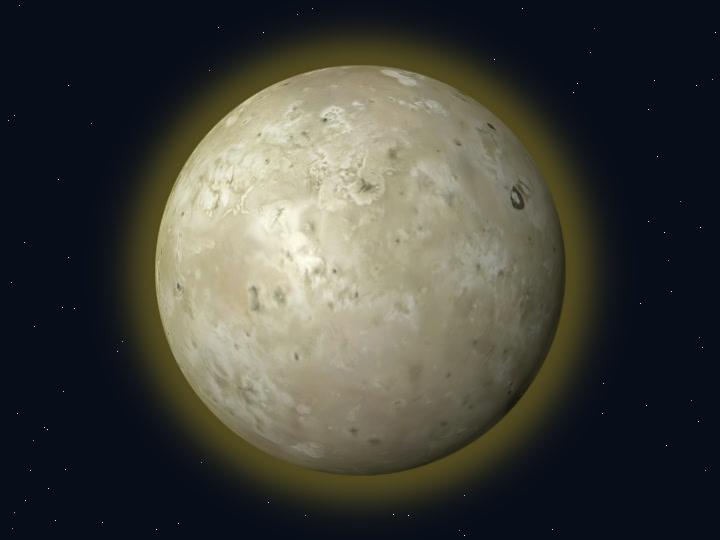
\includegraphics[width=\linewidth,height=4.4cm,keepaspectratio]{imagini/globuri/io.jpg}\\[2pt]
{\scriptsize\itshape\color{orbitarMuted} Vedere 3D a corpului ceresc (\textbf{Io})}
&
\centering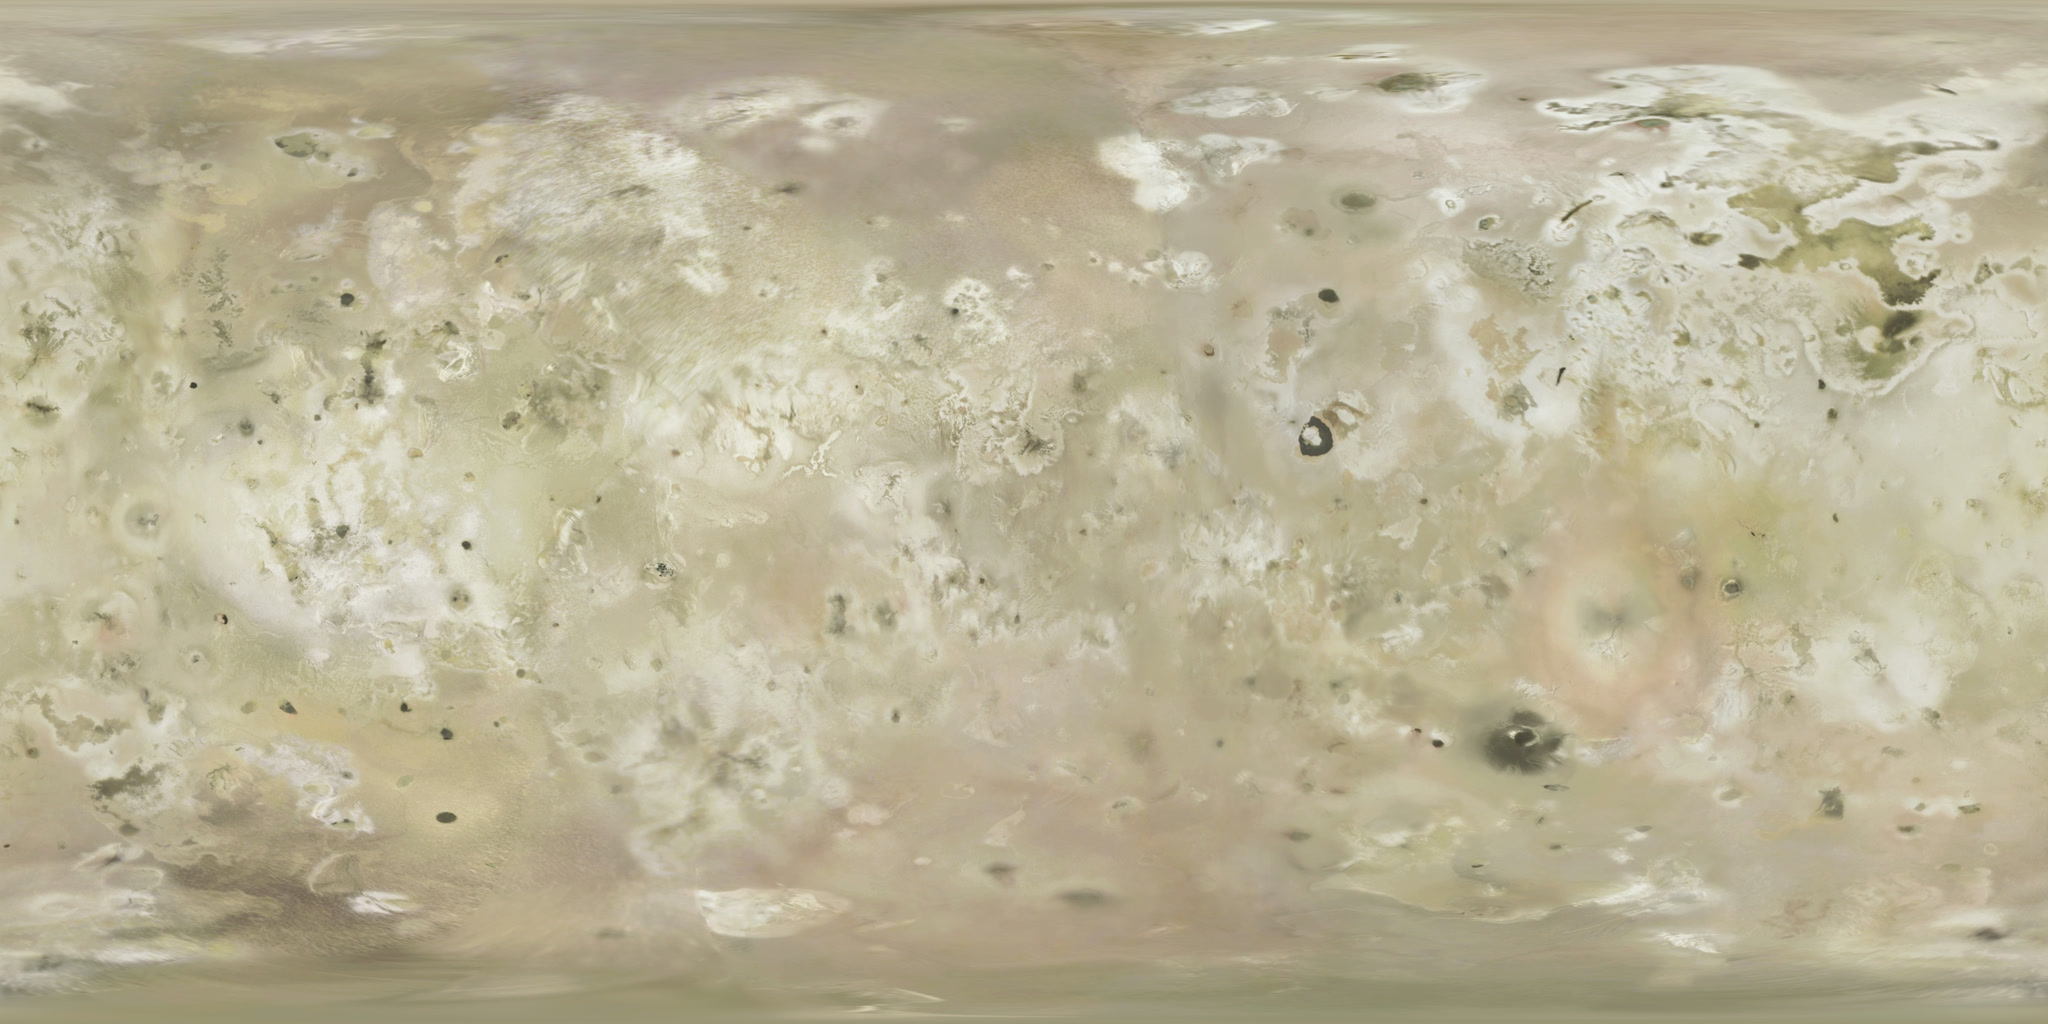
\includegraphics[width=\linewidth,height=4.4cm,keepaspectratio]{../public/textures/hd/io_galileo.jpg}\\[2pt]
{\scriptsize\itshape\color{orbitarMuted} Planiglob desfășurat: Harta vulcanică globală a lunii Io, acoperită cu depozite de sulf și caldere active (sonda NASA Galileo).}
\end{tabular}
\end{center}


\begin{tcolorbox}[orbitardata, title={\textbf{Repere esențiale: Io}}]
\small
\begin{itemize}[leftmargin=1.4em, itemsep=2pt, topsep=2pt]
  \item \textbf{Clasificare și orbită:} Satelit Natural (Lună) (orbitează în jurul: \textbf{Jupiter}) \quad$\bullet$\quad \textbf{Distanță:} 5,204 UA ($\approx$ 779 milioane de kilometri)
  \item \textbf{Dimensiuni și masă:} rază medie 1.821,6 de kilometri \quad$\bullet$\quad masă: 0,015 $\times M_\oplus$
  \item \textbf{Gravitație și regim termic:} 0,183 $\times g_\oplus$ (1,80 m/s$^2$) \quad$\bullet$\quad temperatură medie: -143 $^\circ$C (înclinarea axei: Nespecificată)
  \item \textbf{Ciclu orbital și rotație:} perioadă orbitală (an): 1,769 zile pământești \quad$\bullet$\quad rotație (zi): 42,46 ore (1,77 zile pământești)
  \item \textbf{Durata călătoriei de pe Pământ:} cu viteza luminii ($1c$): \emph{35 de minute}; cu racheta ($50.000$ de kilometri pe oră): \emph{2,5 ani}; cu avionul ($900$ de kilometri pe oră): \emph{80 de ani}; cu mașina ($100$ de kilometri pe oră): \emph{717 ani}.
  \item \textbf{Repere de scară și curiozitate:} Cu petele ei galbene, portocalii și roșii, Io arată exact ca o pizza uriașă cu multă brânză! Jupiter și celelalte luni trag atât de tare de Io încât interiorul ei se frământă și se încălzește ca o bucată de plastilină!
\end{itemize}
\end{tcolorbox}

\subsubsection*{Prezentare generală și profil astrofizic}
Cel mai apropiat dintre cei patru sateliți galileeni ai lui Jupiter suferă o încălzire mareică extremă din cauza rezonanței orbitale 4:2:1 cu Europa și Ganymede. Are peste 400 de vulcani activi, iar jeturile sale eruptive se ridică până la 500 de kilometri altitudine. Io este cea mai vulcanică lume din tot Sistemul Solar! Are sute de vulcani activi care aruncă fântâni uriașe de lavă și sulf până în spațiu. Cu petele ei galbene, portocalii și roșii, Io arată exact ca o pizza uriașă cu multă brânză!

\subsubsection*{Alcătuirea fizică și structura internă}
Privind în profunzimea sa, alcătuirea fizică este organizată pe mai multe straturi și regiuni distincte, fiecare având un rol bine definit în evoluția și dinamica acestui obiect cosmic. În primul rând se remarcă \textbf{Nucleu de fier și sulfură de fier}, care reprezintă aproximativ 20\% din masa satelitului. În strânsă legătură cu această componentă se află \textbf{Manta de silicați și ocean de magmă}, un strat global de magmă topită la 50 de kilometri sub scoarță, alimentat de frecarea mareică. În completarea acestui ansamblu întâlnim \textbf{Scoarță bogată în sulf}, câmpii de lavă și caldere vulcanice precum Loki Patera, fără cratere de impact vizibile.

\subsubsection*{Observații astronomice și istoricul explorării}
Descoperită de Galileo Galilei în 1610; vulcanismul ei activ a fost observat pentru prima dată de sonda Voyager 1 în 1979. Jupiter și celelalte luni trag atât de tare de Io încât interiorul ei se frământă și se încălzește ca o bucată de plastilină!

\vspace{6pt}
\begin{tcolorbox}[orbitarquiz, title={\textbf{Întrebare de verificare \#10: Io}}]
\textbf{Ce fenomen provoacă activitatea vulcanică extremă de pe satelitul Io?}
\begin{itemize}[leftmargin=2.2em, itemsep=2pt, topsep=4pt]
  \item[$\square$ \textbf{A.}] Căldura directă de la Soare
  \item[$\square$ \textbf{B.}] Încălzirea mareică produsă de gravitația lui Jupiter și a lunilor vecine
  \item[$\square$ \textbf{C.}] Impactul continuu cu asteroizi
  \item[$\square$ \textbf{D.}] Fuziunea nucleară
\end{itemize}
\vspace{2pt}
{\footnotesize\color{orbitarMuted}\textbf{Răspuns corect:} \textbf{B} (Încălzirea mareică produsă de gravitația lui Jupiter și a lunilor vecine). \emph{Forțele mareice uriașe ale lui Jupiter deformează continuu interiorul lui Io, generând căldură prin frecare internă.}}
\end{tcolorbox}
\clearpage


\subsection{Europa}
\label{sec:body-europa}
\vspace{-4pt}
{\large\itshape\color{orbitarAccent} Luna înghețată a lui Jupiter cu un ocean ascuns}\\[4pt]


\begin{center}
\begin{tabular}{@{}m{0.44\textwidth}@{\hspace{0.03\textwidth}}m{0.51\textwidth}@{}}
\centering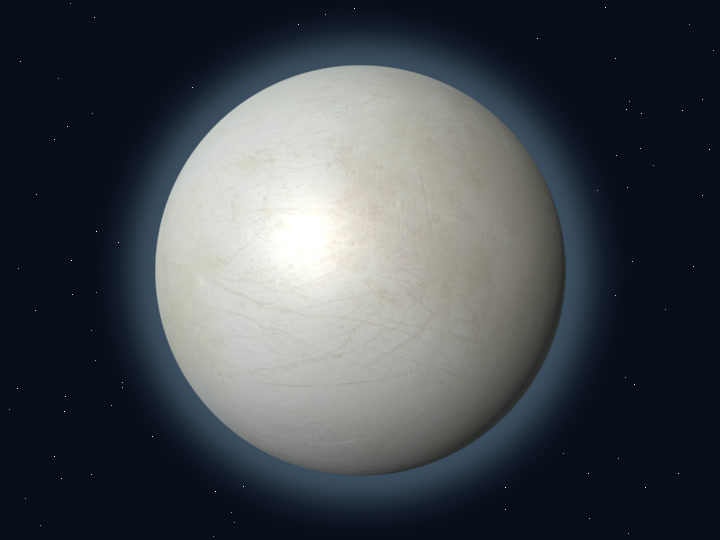
\includegraphics[width=\linewidth,height=4.4cm,keepaspectratio]{imagini/globuri/europa.jpg}\\[2pt]
{\scriptsize\itshape\color{orbitarMuted} Vedere 3D a corpului ceresc (\textbf{Europa})}
&
\centering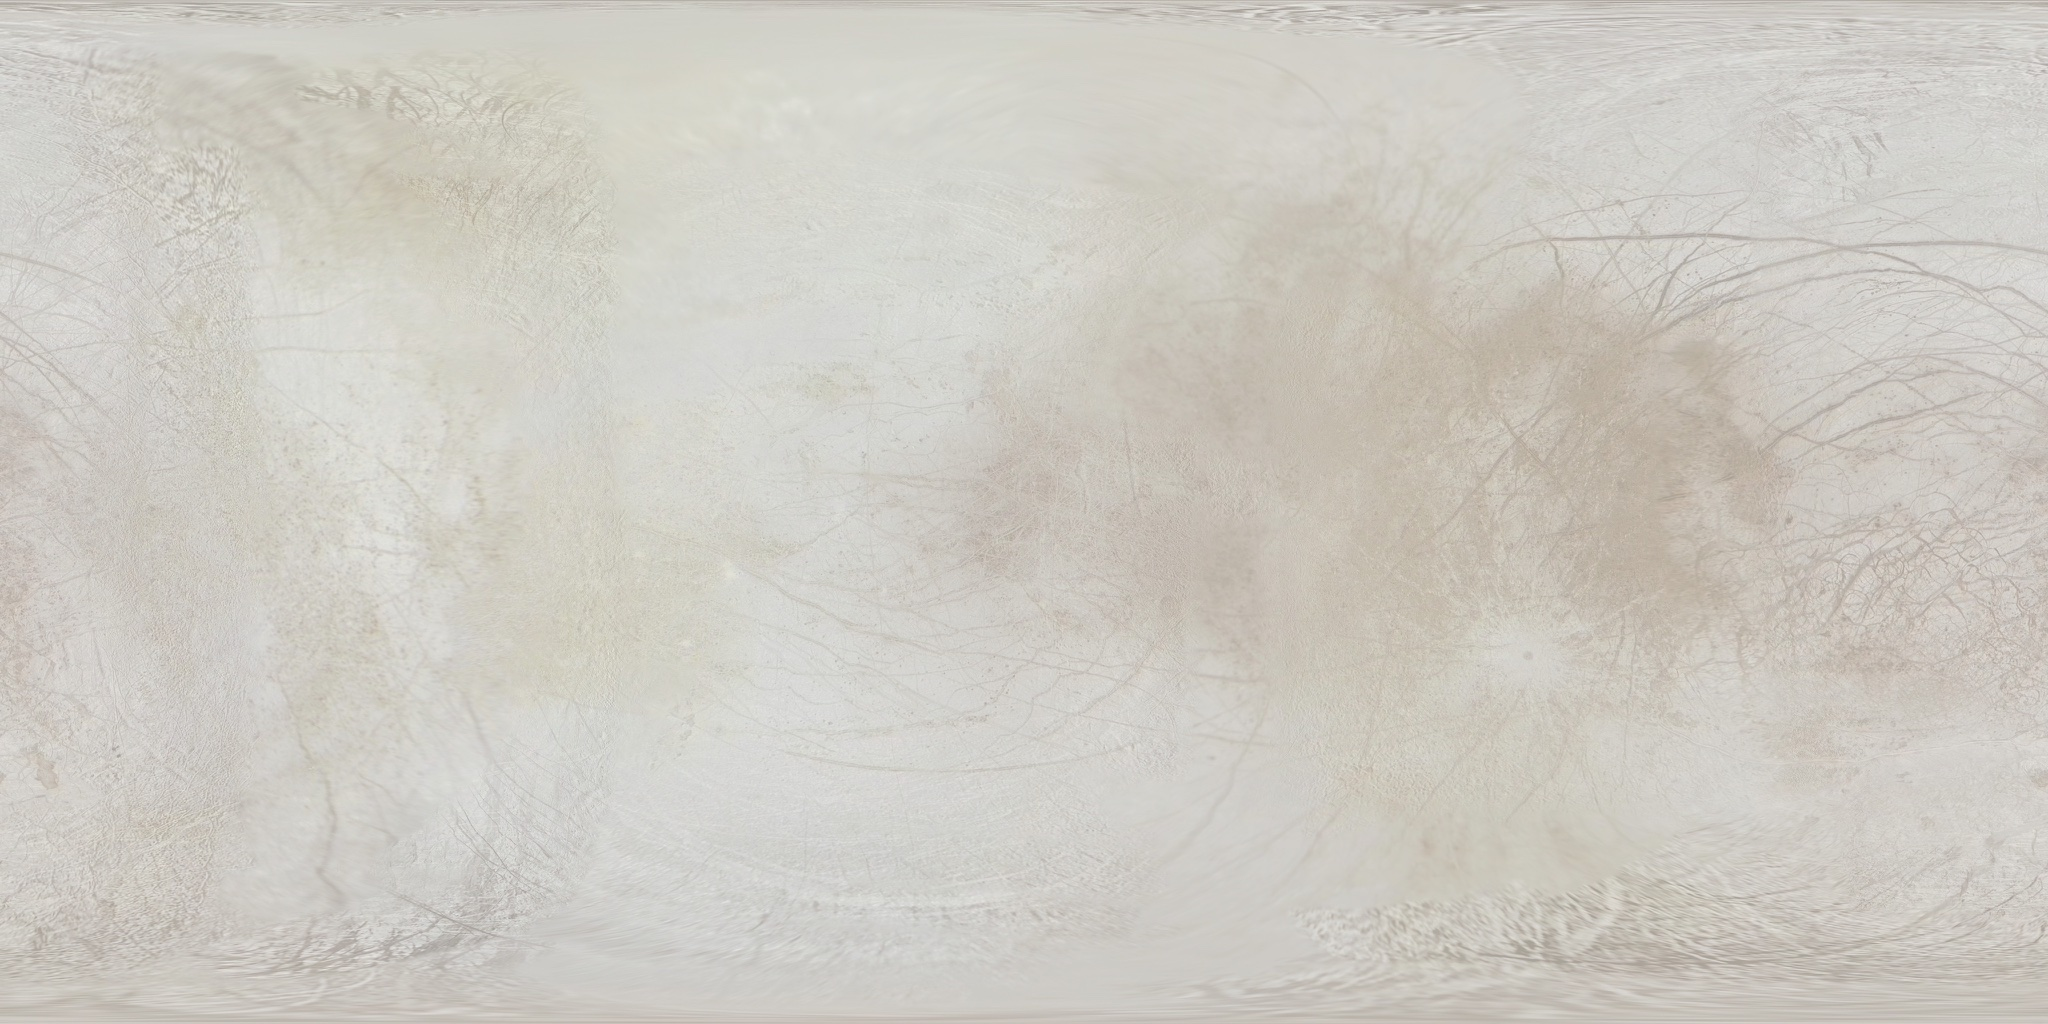
\includegraphics[width=\linewidth,height=4.4cm,keepaspectratio]{../public/textures/hd/europa_galileo.jpg}\\[2pt]
{\scriptsize\itshape\color{orbitarMuted} Planiglob desfășurat: Scoarța de gheață brăzdată de fracturi roșiatice (lineae) a lunii Europa, sub care se află un ocean global (NASA Galileo).}
\end{tabular}
\end{center}


\begin{tcolorbox}[orbitardata, title={\textbf{Repere esențiale: Europa}}]
\small
\begin{itemize}[leftmargin=1.4em, itemsep=2pt, topsep=2pt]
  \item \textbf{Clasificare și orbită:} Satelit Natural (Lună) (orbitează în jurul: \textbf{Jupiter}) \quad$\bullet$\quad \textbf{Distanță:} 5,204 UA ($\approx$ 779 milioane de kilometri)
  \item \textbf{Dimensiuni și masă:} rază medie 1.560,8 de kilometri \quad$\bullet$\quad masă: 0,008 $\times M_\oplus$
  \item \textbf{Gravitație și regim termic:} 0,134 $\times g_\oplus$ (1,31 m/s$^2$) \quad$\bullet$\quad temperatură medie: -160 $^\circ$C (înclinarea axei: Nespecificată)
  \item \textbf{Ciclu orbital și rotație:} perioadă orbitală (an): 3,551 zile pământești \quad$\bullet$\quad rotație (zi): 85,22 ore (3,55 zile pământești)
  \item \textbf{Durata călătoriei de pe Pământ:} cu viteza luminii ($1c$): \emph{35 de minute}; cu racheta ($50.000$ de kilometri pe oră): \emph{2,5--5 ani}; cu avionul ($900$ de kilometri pe oră): \emph{80 de ani}; cu mașina ($100$ de kilometri pe oră): \emph{717 ani}.
  \item \textbf{Repere de scară și curiozitate:} Europa este ca un ou de ciocolată cu surprize: tare și înghețată la exterior, dar cu un ocean adânc înăuntru! Deși Europa este mai mică decât Luna noastră, oceanul ei ascuns are de două ori mai multă apă decât toate oceanele Pământului!
\end{itemize}
\end{tcolorbox}

\subsubsection*{Prezentare generală și profil astrofizic}
Europa are cea mai netedă suprafață din Sistemul Solar, brăzdată de fracturi roșiatice numite \guillemotleft{}lineae\guillemotright{}. Sub crusta de gheață de 15--25 de kilometri grosime se află un ocean global de apă lichidă cu o adâncime estimată la 100 de kilometri, fiind unul dintre principalele locuri căutate pentru viață extraterestră. Europa este o lună acoperită cu un patinoar neted de gheață! Sub această coajă înghețată se ascunde un ocean uriaș de apă sărată. Europa este ca un ou de ciocolată cu surprize: tare și înghețată la exterior, dar cu un ocean adânc înăuntru!

\subsubsection*{Alcătuirea fizică și structura internă}
Privind în profunzimea sa, alcătuirea fizică este organizată pe mai multe straturi și regiuni distincte, fiecare având un rol bine definit în evoluția și dinamica acestui obiect cosmic. În primul rând se remarcă \textbf{Nucleu metalic și manta stâncoasă}, unde contactul direct dintre ocean și mantaua stâncoasă permite existența izvoarelor hidrotermale. În strânsă legătură cu această componentă se află \textbf{Ocean global subglaciar}, apă sărată menținută lichidă de încălzirea mareică joviană. În completarea acestui ansamblu întâlnim \textbf{Crustă activă de gheață}, plăci de gheață în mișcare și posibile gheizere de vapori de apă.

\subsubsection*{Observații astronomice și istoricul explorării}
Studiată de Galileo și Juno, fiind ținta principală a misiunilor JUICE (ESA) și Europa Clipper (NASA). Deși Europa este mai mică decât Luna noastră, oceanul ei ascuns are de două ori mai multă apă decât toate oceanele Pământului!

\vspace{6pt}
\begin{tcolorbox}[orbitarquiz, title={\textbf{Întrebare de verificare \#11: Europa}}]
\textbf{De ce sunt oamenii de știință atât de interesați de satelitul Europa?}
\begin{itemize}[leftmargin=2.2em, itemsep=2pt, topsep=4pt]
  \item[$\square$ \textbf{A.}] Are păduri tropicale
  \item[$\square$ \textbf{B.}] Adăpostește sub gheață un ocean global de apă lichidă care ar putea susține viață
  \item[$\square$ \textbf{C.}] Este cel mai fierbinte corp din Sistemul Solar
  \item[$\square$ \textbf{D.}] Are inele strălucitoare
\end{itemize}
\vspace{2pt}
{\footnotesize\color{orbitarMuted}\textbf{Răspuns corect:} \textbf{B} (Adăpostește sub gheață un ocean global de apă lichidă care ar putea susține viață). \emph{Oceanul subglaciar al Europei, aflat în contact cu un fund oceanic stâncos, oferă ingredientele esențiale pentru potențiale ecosisteme.}}
\end{tcolorbox}
\clearpage


\subsection{Ganymede}
\label{sec:body-ganymede}
\vspace{-4pt}
{\large\itshape\color{orbitarAccent} Cel mai mare satelit natural din Sistemul Solar}\\[4pt]


\begin{center}
\begin{tabular}{@{}m{0.44\textwidth}@{\hspace{0.03\textwidth}}m{0.51\textwidth}@{}}
\centering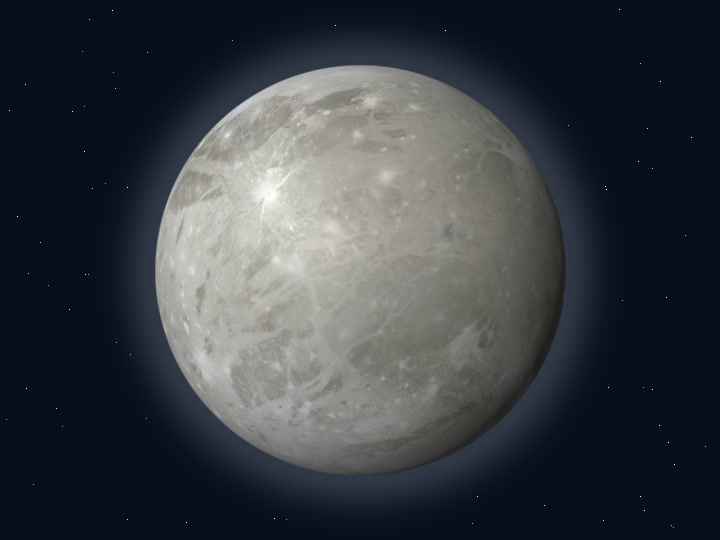
\includegraphics[width=\linewidth,height=4.4cm,keepaspectratio]{imagini/globuri/ganymede.jpg}\\[2pt]
{\scriptsize\itshape\color{orbitarMuted} Vedere 3D a corpului ceresc (\textbf{Ganymede})}
&
\centering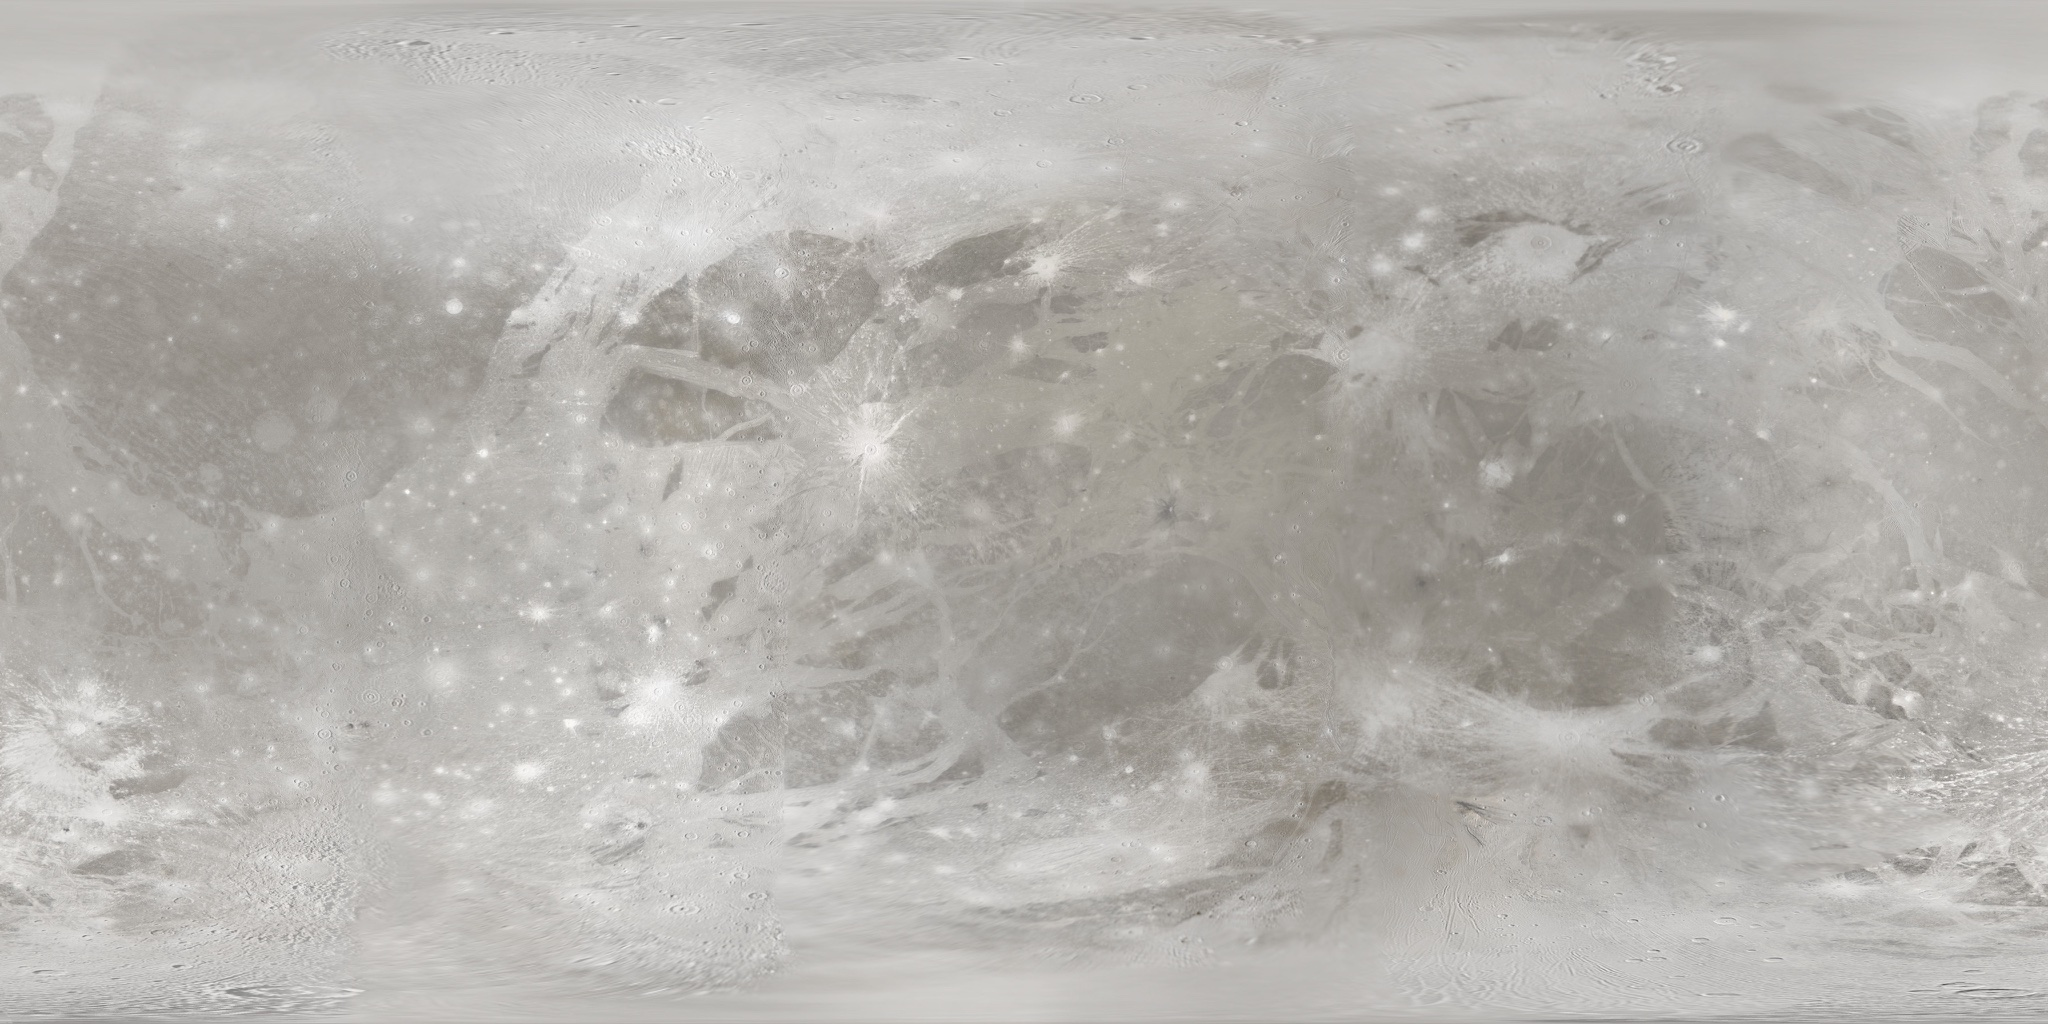
\includegraphics[width=\linewidth,height=4.4cm,keepaspectratio]{../public/textures/hd/ganymede_galileo.jpg}\\[2pt]
{\scriptsize\itshape\color{orbitarMuted} Planiglob desfășurat: Harta celui mai mare satelit din Sistemul Solar, Ganymede, obținută de misiunile NASA Voyager și Galileo.}
\end{tabular}
\end{center}


\begin{tcolorbox}[orbitardata, title={\textbf{Repere esențiale: Ganymede}}]
\small
\begin{itemize}[leftmargin=1.4em, itemsep=2pt, topsep=2pt]
  \item \textbf{Clasificare și orbită:} Satelit Natural (Lună) (orbitează în jurul: \textbf{Jupiter}) \quad$\bullet$\quad \textbf{Distanță:} 5,204 UA ($\approx$ 779 milioane de kilometri)
  \item \textbf{Dimensiuni și masă:} rază medie 2.631,2 de kilometri \quad$\bullet$\quad masă: 0,025 $\times M_\oplus$
  \item \textbf{Gravitație și regim termic:} 0,146 $\times g_\oplus$ (1,43 m/s$^2$) \quad$\bullet$\quad temperatură medie: -163 $^\circ$C (înclinarea axei: Nespecificată)
  \item \textbf{Ciclu orbital și rotație:} perioadă orbitală (an): 7,155 zile pământești \quad$\bullet$\quad rotație (zi): 171,70 ore (7,15 zile pământești)
  \item \textbf{Durata călătoriei de pe Pământ:} cu viteza luminii ($1c$): \emph{35 de minute}; cu racheta ($50.000$ de kilometri pe oră): \emph{2,5--5 ani}; cu avionul ($900$ de kilometri pe oră): \emph{80 de ani}; cu mașina ($100$ de kilometri pe oră): \emph{717 ani}.
  \item \textbf{Repere de scară și curiozitate:} Dacă Ganymede s-ar învârti direct în jurul Soarelui în loc de Jupiter, ar fi numită fără îndoială o planetă! Ganymede este singura lună din Sistemul Solar care are propriul ei scut magnetic și propriile aurore polare!
\end{itemize}
\end{tcolorbox}

\subsubsection*{Prezentare generală și profil astrofizic}
Cu un diametru de 5.262 de kilometri, Ganymede este cel mai mare satelit din Sistemul Solar și singurul cunoscut care posedă o magnetosferă intrinsecă, generată de convecția din nucleul său de fier lichid. Ganymede este campionul tuturor lunilor! Este atât de mare încât depășește chiar și planeta Mercur în dimensiune. Dacă Ganymede s-ar învârti direct în jurul Soarelui în loc de Jupiter, ar fi numită fără îndoială o planetă!

\subsubsection*{Alcătuirea fizică și structura internă}
Privind în profunzimea sa, alcătuirea fizică este organizată pe mai multe straturi și regiuni distincte, fiecare având un rol bine definit în evoluția și dinamica acestui obiect cosmic. În primul rând se remarcă \textbf{Nucleu de fier lichid}, care generează un câmp magnetic propriu în interiorul magnetosferei uriașe a lui Jupiter. În strânsă legătură cu această componentă se află \textbf{Straturi alternante de gheață și oceane}, unde modelele indică un ocean subteran uriaș prins între straturi de gheață de înaltă presiune. În completarea acestui ansamblu întâlnim \textbf{Scoarță mixtă}, regiuni întunecate străvechi craterizate și terenuri mai tinere, brăzdate de șanțuri tectonice.

\subsubsection*{Observații astronomice și istoricul explorării}
Descoperită în 1610 de Galileo Galilei; sonda europeană JUICE va deveni în 2034 prima navă care va intra pe orbita lui Ganymede. Ganymede este singura lună din Sistemul Solar care are propriul ei scut magnetic și propriile aurore polare!

\vspace{6pt}
\begin{tcolorbox}[orbitarquiz, title={\textbf{Întrebare de verificare \#12: Ganymede}}]
\textbf{Prin ce este Ganymede unic printre toți sateliții naturali din Sistemul Solar?}
\begin{itemize}[leftmargin=2.2em, itemsep=2pt, topsep=4pt]
  \item[$\square$ \textbf{A.}] Este cel mai mare satelit (mai mare decât Mercur) și are câmp magnetic propriu
  \item[$\square$ \textbf{B.}] Are vulcani de lavă fierbinte
  \item[$\square$ \textbf{C.}] Orbitează în jurul lui Marte
  \item[$\square$ \textbf{D.}] Este compus doar din gaz
\end{itemize}
\vspace{2pt}
{\footnotesize\color{orbitarMuted}\textbf{Răspuns corect:} \textbf{A} (Este cel mai mare satelit (mai mare decât Mercur) și are câmp magnetic propriu). \emph{Ganymede depășește în diametru planeta Mercur și este singurul satelit cu o magnetosferă proprie.}}
\end{tcolorbox}
\clearpage


\subsection{Callisto}
\label{sec:body-callisto}
\vspace{-4pt}
{\large\itshape\color{orbitarAccent} Lumea străveche de gheață și cratere a lui Jupiter}\\[4pt]


\begin{center}
\begin{tabular}{@{}m{0.44\textwidth}@{\hspace{0.03\textwidth}}m{0.51\textwidth}@{}}
\centering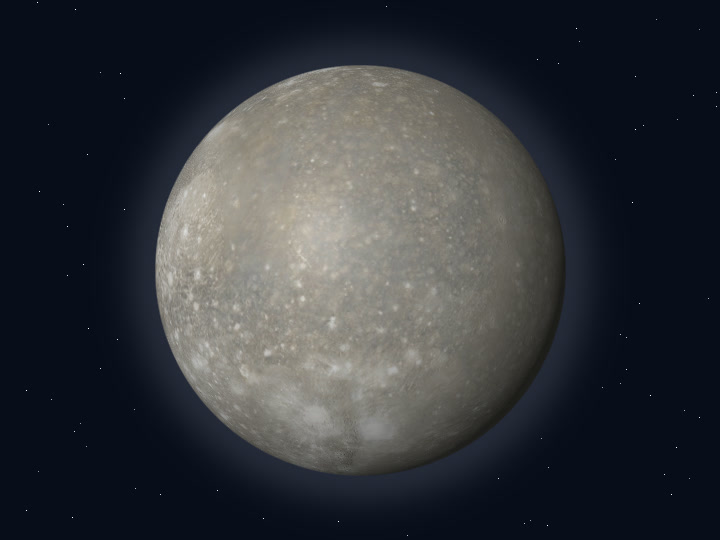
\includegraphics[width=\linewidth,height=4.4cm,keepaspectratio]{imagini/globuri/callisto.jpg}\\[2pt]
{\scriptsize\itshape\color{orbitarMuted} Vedere 3D a corpului ceresc (\textbf{Callisto})}
&
\centering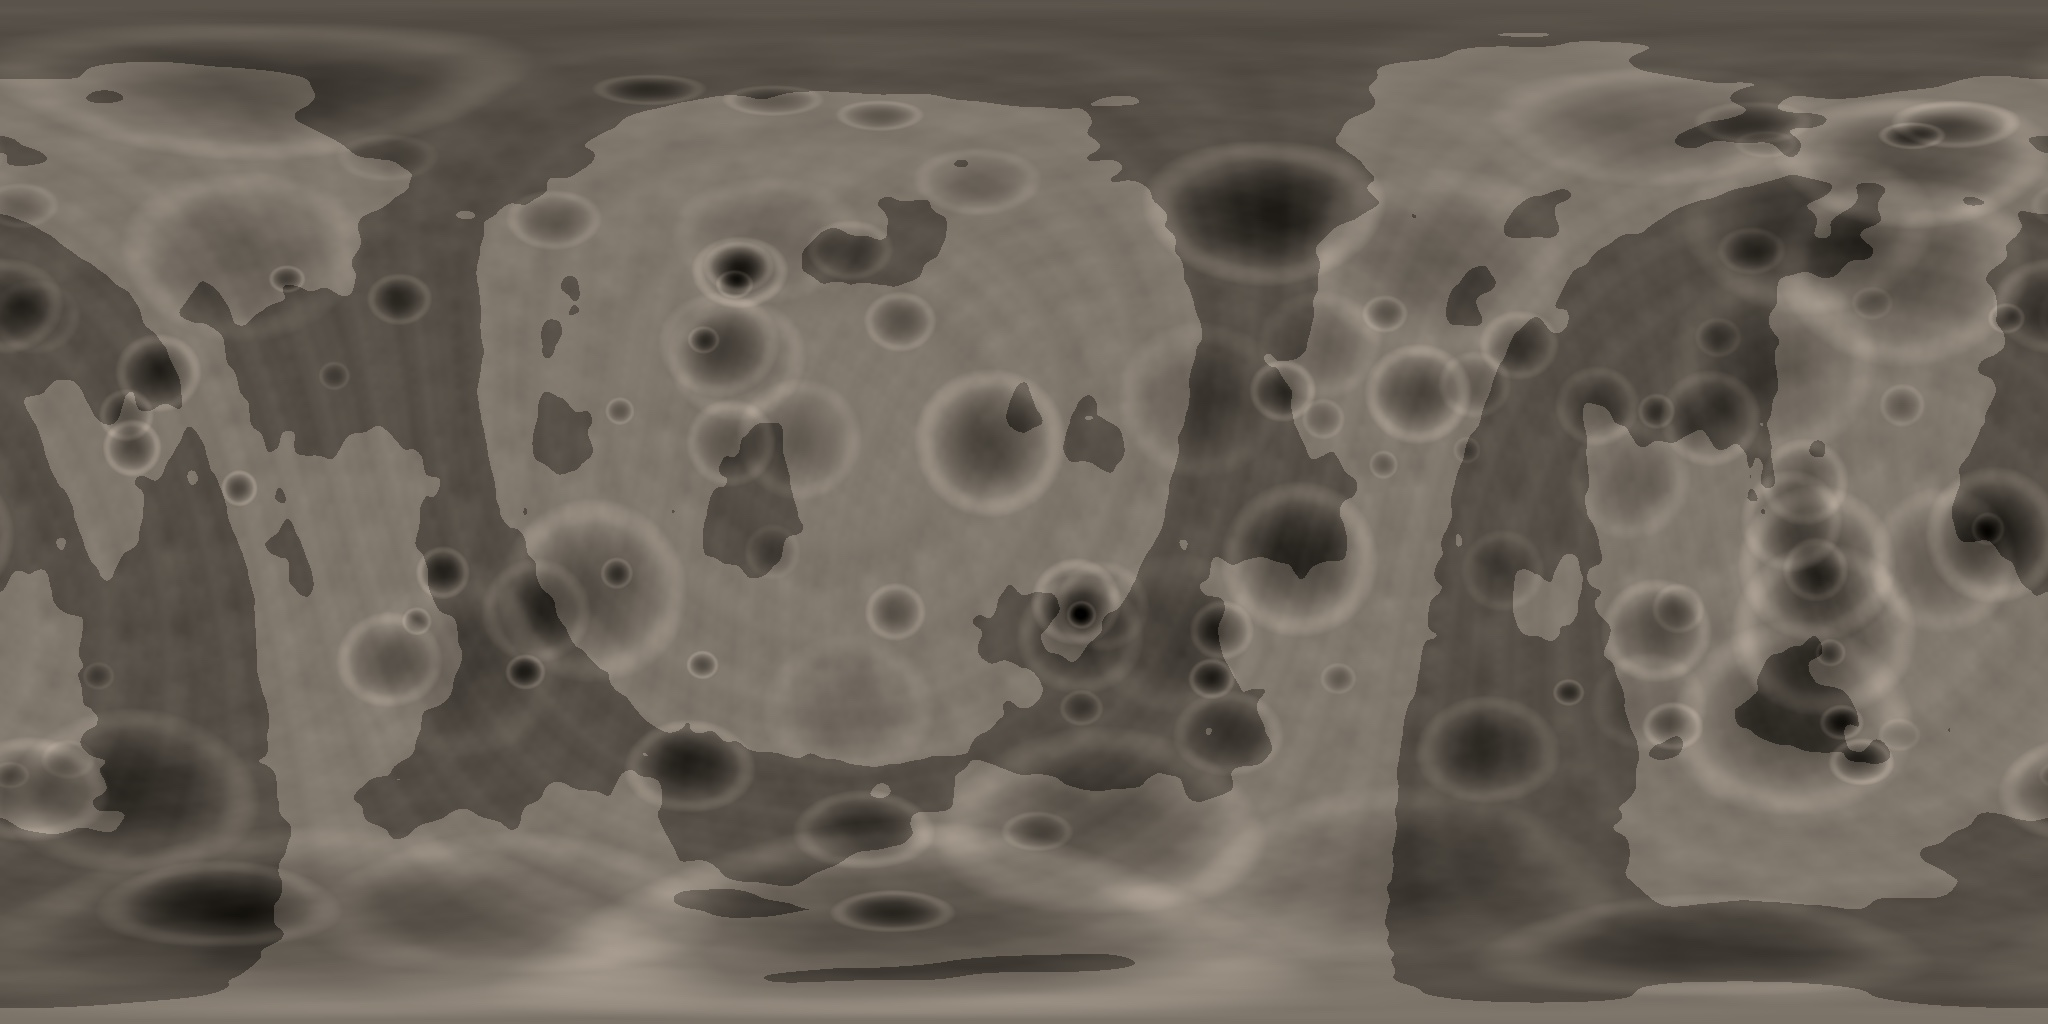
\includegraphics[width=\linewidth,height=4.4cm,keepaspectratio]{../public/textures/hd/callisto_galileo.jpg}\\[2pt]
{\scriptsize\itshape\color{orbitarMuted} Planiglob desfășurat: Suprafața străveche a lunii Callisto și bazinul multi-inelar Valhalla (date NASA Galileo).}
\end{tabular}
\end{center}


\begin{tcolorbox}[orbitardata, title={\textbf{Repere esențiale: Callisto}}]
\small
\begin{itemize}[leftmargin=1.4em, itemsep=2pt, topsep=2pt]
  \item \textbf{Clasificare și orbită:} Satelit Natural (Lună) (orbitează în jurul: \textbf{Jupiter}) \quad$\bullet$\quad \textbf{Distanță:} 5,204 UA ($\approx$ 779 milioane de kilometri)
  \item \textbf{Dimensiuni și masă:} rază medie 2.410,3 kilometri \quad$\bullet$\quad masă: 0,018 $\times M_\oplus$
  \item \textbf{Gravitație și regim termic:} 0,126 $\times g_\oplus$ (1,24 m/s$^2$) \quad$\bullet$\quad temperatură medie: -139 $^\circ$C (înclinarea axei: Nespecificată)
  \item \textbf{Ciclu orbital și rotație:} perioadă orbitală (an): 16,689 zile pământești \quad$\bullet$\quad rotație (zi): 400,50 ore (16,69 zile pământești)
  \item \textbf{Durata călătoriei de pe Pământ:} cu viteza luminii ($1c$): \emph{35 de minute}; cu racheta ($50.000$ de kilometri pe oră): \emph{2,5--5 ani}; cu avionul ($900$ de kilometri pe oră): \emph{80 de ani}; cu mașina ($100$ de kilometri pe oră): \emph{717 ani}.
  \item \textbf{Repere de scară și curiozitate:} Callisto arată ca un glob de Crăciun întunecat, presărat cu mii de scântei albe acolo unde au căzut meteoriți! Fiind mai departe de radiațiile puternice ale lui Jupiter, Callisto este locul preferat de ingineri pentru o viitoare bază umană!
\end{itemize}
\end{tcolorbox}

\subsubsection*{Prezentare generală și profil astrofizic}
Al treilea satelit ca mărime din Sistemul Solar (aproape cât Mercur) nu participă la rezonanța orbitală a celorlalte trei luni galileene, motiv pentru care nu a suferit încălzire mareică intensă, păstrând o arhivă geologică intactă de 4 miliarde de ani. Callisto este a patra lună mare a lui Jupiter și are cea mai veche suprafață din Sistemul Solar, plină de cratere strălucitoare de gheață! Callisto arată ca un glob de Crăciun întunecat, presărat cu mii de scântei albe acolo unde au căzut meteoriți!

\subsubsection*{Alcătuirea fizică și structura internă}
Privind în profunzimea sa, alcătuirea fizică este organizată pe mai multe straturi și regiuni distincte, fiecare având un rol bine definit în evoluția și dinamica acestui obiect cosmic. În primul rând se remarcă \textbf{Interior parțial diferențiat}, un amestec comprimat de rocă și gheață, fără un nucleu metalic mare complet separat. În strânsă legătură cu această componentă se află \textbf{Posibil ocean sărat la adâncime}, detectat indirect prin variațiile câmpului magnetic indus. În completarea acestui ansamblu întâlnim \textbf{Litosferă străveche}, dominată de Bazinul Valhalla, o structură de impact cu inele concentrice de 3.800 de kilometri diametru.

\subsubsection*{Observații astronomice și istoricul explorării}
Fotografiată în detaliu de Voyager 1/2 și Galileo; va fi survolată de 21 de ori de sonda JUICE. Fiind mai departe de radiațiile puternice ale lui Jupiter, Callisto este locul preferat de ingineri pentru o viitoare bază umană!

\vspace{6pt}
\begin{tcolorbox}[orbitarquiz, title={\textbf{Întrebare de verificare \#13: Callisto}}]
\textbf{Cum se numește uriașul bazin de impact cu inele concentrice de pe Callisto?}
\begin{itemize}[leftmargin=2.2em, itemsep=2pt, topsep=4pt]
  \item[$\square$ \textbf{A.}] Valhalla
  \item[$\square$ \textbf{B.}] Caloris
  \item[$\square$ \textbf{C.}] Olympus
  \item[$\square$ \textbf{D.}] Sputnik
\end{itemize}
\vspace{2pt}
{\footnotesize\color{orbitarMuted}\textbf{Răspuns corect:} \textbf{A} (Valhalla). \emph{Bazinul Valhalla este cel mai mare crater multi-inelar de pe Callisto, având un diametru de aproape 3.800 de kilometri.}}
\end{tcolorbox}
\clearpage


\section{Saturn}
\label{sec:body-saturn}
\vspace{-4pt}
{\large\itshape\color{orbitarAccent} Bijuteria Sistemului Solar, încoronată cu inele de gheață}\\[4pt]


\begin{center}
\begin{tabular}{@{}m{0.44\textwidth}@{\hspace{0.03\textwidth}}m{0.51\textwidth}@{}}
\centering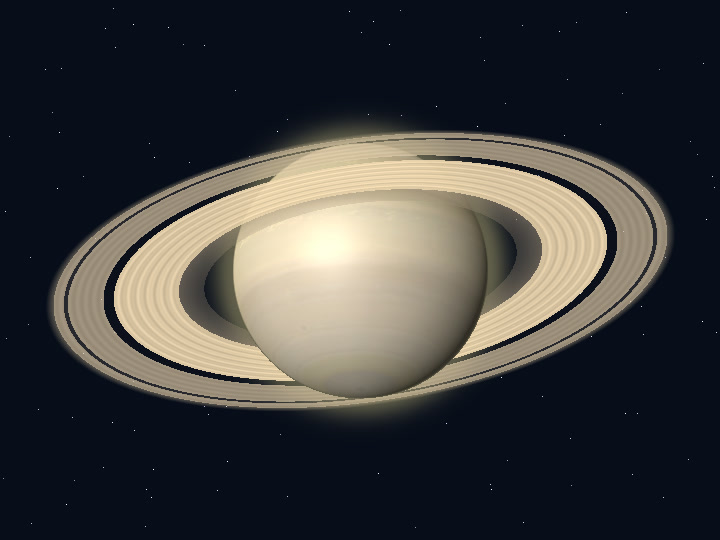
\includegraphics[width=\linewidth,height=4.4cm,keepaspectratio]{imagini/globuri/saturn.jpg}\\[2pt]
{\scriptsize\itshape\color{orbitarMuted} Vedere 3D a corpului ceresc (\textbf{Saturn})}
&
\centering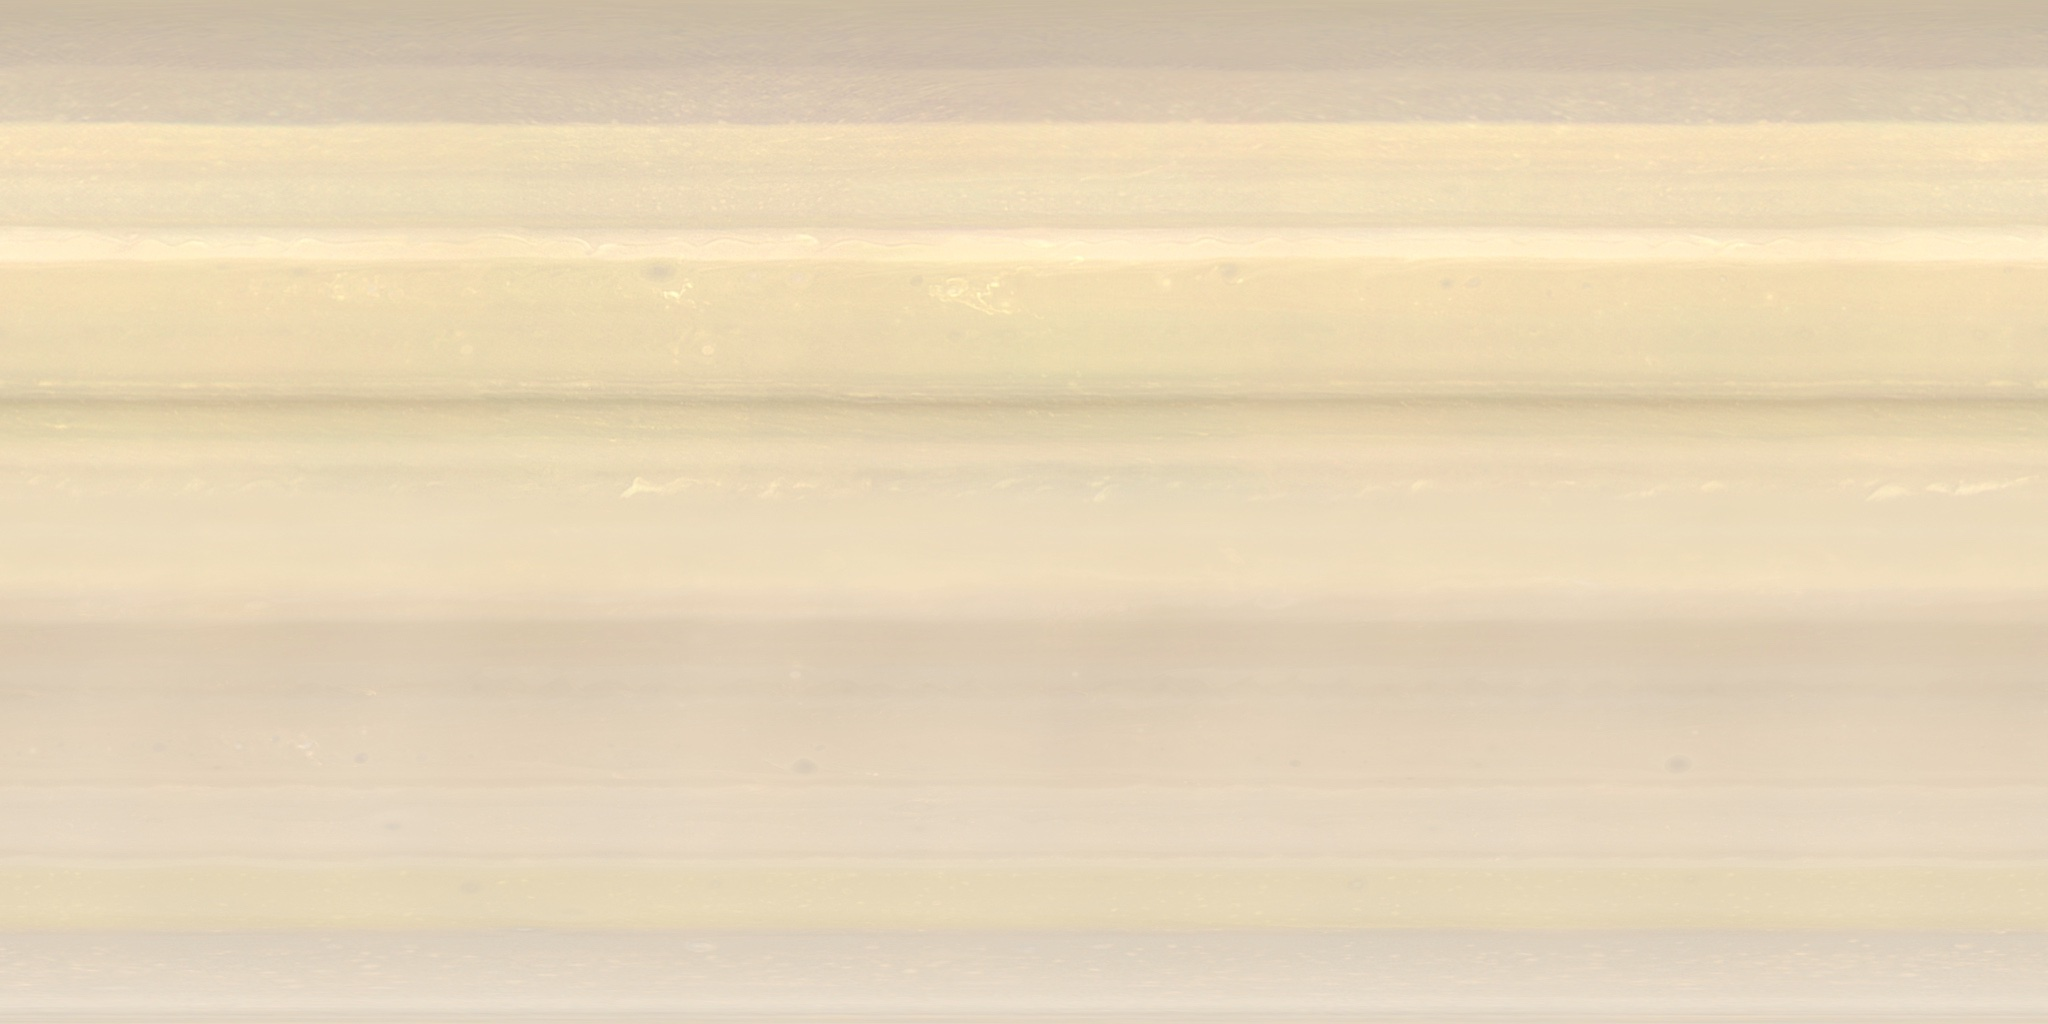
\includegraphics[width=\linewidth,height=4.4cm,keepaspectratio]{../public/textures/hd/saturn_cassini_albedo.jpg}\\[2pt]
{\scriptsize\itshape\color{orbitarMuted} Planiglob desfășurat: Harta benzilor atmosferice aurii ale gigantului gazos Saturn (date NASA/ESA Cassini).}
\end{tabular}
\end{center}


\begin{tcolorbox}[orbitardata, title={\textbf{Repere esențiale: Saturn}}]
\small
\begin{itemize}[leftmargin=1.4em, itemsep=2pt, topsep=2pt]
  \item \textbf{Clasificare și orbită:} Gigant Gazos \quad$\bullet$\quad \textbf{Distanță:} 9,582 UA ($\approx$ 1.433 milioane de kilometri)
  \item \textbf{Dimensiuni și masă:} rază medie 58.232 de kilometri \quad$\bullet$\quad masă: 95,160 $\times M_\oplus$
  \item \textbf{Gravitație și regim termic:} 1,060 $\times g_\oplus$ (10,40 m/s$^2$) \quad$\bullet$\quad temperatură medie: -140 $^\circ$C (înclinarea axei: 26,73$^\circ$)
  \item \textbf{Ciclu orbital și rotație:} perioadă orbitală (an): 10.759,22 zile ($\approx$ 29,46 ani pământești) \quad$\bullet$\quad rotație (zi): 10,70 ore (0,45 zile pământești)
  \item \textbf{Durata călătoriei de pe Pământ:} cu viteza luminii ($1c$): \emph{1 oră și 11 minute}; cu racheta ($50.000$ de kilometri pe oră): \emph{3 până la 7 ani}; cu avionul ($900$ de kilometri pe oră): \emph{160 de ani}; cu mașina ($100$ de kilometri pe oră): \emph{1.450 de ani}.
  \item \textbf{Repere de scară și curiozitate:} Saturn este atât de ușor pentru mărimea lui încât, dacă am avea o cadă cu apă destul de mare, planeta ar pluti! La polul nord al lui Saturn există un vârtej de nori cu o formă geometrică perfectă de hexagon!
\end{itemize}
\end{tcolorbox}

\subsubsection*{Prezentare generală și profil astrofizic}
Al doilea gigant gazos ca mărime are o densitate medie de doar 0,687 g/cm$^3$ (mai mică decât a apei). Sistemul său principal de inele (A, B, C) are o lățime de 282.000 de kilometri, dar o grosime medie de numai 10--30 de metri. Saturn este cea mai ușor de recunoscut planetă datorită inelelor sale strălucitoare! Aceste inele sunt făcute din miliarde de bulgări de gheață și praf cosmic. Saturn este atât de ușor pentru mărimea lui încât, dacă am avea o cadă cu apă destul de mare, planeta ar pluti!

\subsubsection*{Alcătuirea fizică și structura internă}
Privind în profunzimea sa, alcătuirea fizică este organizată pe mai multe straturi și regiuni distincte, fiecare având un rol bine definit în evoluția și dinamica acestui obiect cosmic. În primul rând se remarcă \textbf{Nucleu dens stâncos-metalic}, de 9--22 de ori masa Pământului, înconjurat de hidrogen metalic lichid. În strânsă legătură cu această componentă se află \textbf{Atmosferă aurie cu vânturi de 1.800 kilometri pe oră}, dominată de hidrogen și heliu, cu un jet-stream hexagonal persistent la polul nord. În completarea acestui ansamblu întâlnim \textbf{Sistemul de Inele}, compus 99\% din gheață pură de apă, cu dimensiuni de la granule microscopice la blocuri de câțiva metri.

\subsubsection*{Observații astronomice și istoricul explorării}
Vizitată de Pioneer 11 și Voyager 1/2, apoi explorată în detaliu timp de 13 ani de misiunea istorică Cassini-Huygens (2004--2017). La polul nord al lui Saturn există un vârtej de nori cu o formă geometrică perfectă de hexagon!

\vspace{6pt}
\begin{tcolorbox}[orbitarquiz, title={\textbf{Întrebare de verificare \#14: Saturn}}]
\textbf{Din ce sunt alcătuite în principal celebrele inele ale lui Saturn?}
\begin{itemize}[leftmargin=2.2em, itemsep=2pt, topsep=4pt]
  \item[$\square$ \textbf{A.}] Din inele solide de metal
  \item[$\square$ \textbf{B.}] Din gaze colorate
  \item[$\square$ \textbf{C.}] Din miliarde de fragmente de gheață și rocă
  \item[$\square$ \textbf{D.}] Din lavă vulcanică înghețată
\end{itemize}
\vspace{2pt}
{\footnotesize\color{orbitarMuted}\textbf{Răspuns corect:} \textbf{C} (Din miliarde de fragmente de gheață și rocă). \emph{Inelele lui Saturn nu sunt solide, ci sunt formate din nenumărate particule și blocuri de gheață care orbitează independent planeta.}}
\end{tcolorbox}
\clearpage


\subsection{Mimas}
\label{sec:body-mimas}
\vspace{-4pt}
{\large\itshape\color{orbitarAccent} Luna înghețată a lui Saturn cu craterul gigant Herschel}\\[4pt]


\begin{center}
\begin{tabular}{@{}m{0.44\textwidth}@{\hspace{0.03\textwidth}}m{0.51\textwidth}@{}}
\centering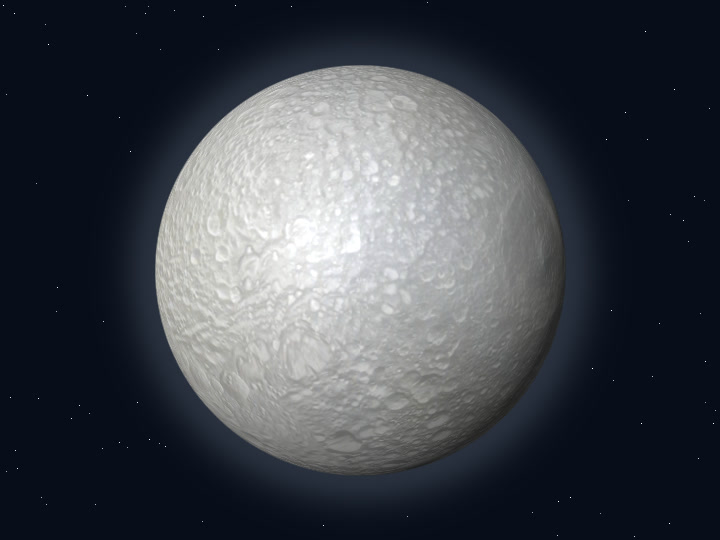
\includegraphics[width=\linewidth,height=4.4cm,keepaspectratio]{imagini/globuri/mimas.jpg}\\[2pt]
{\scriptsize\itshape\color{orbitarMuted} Vedere 3D a corpului ceresc (\textbf{Mimas})}
&
\centering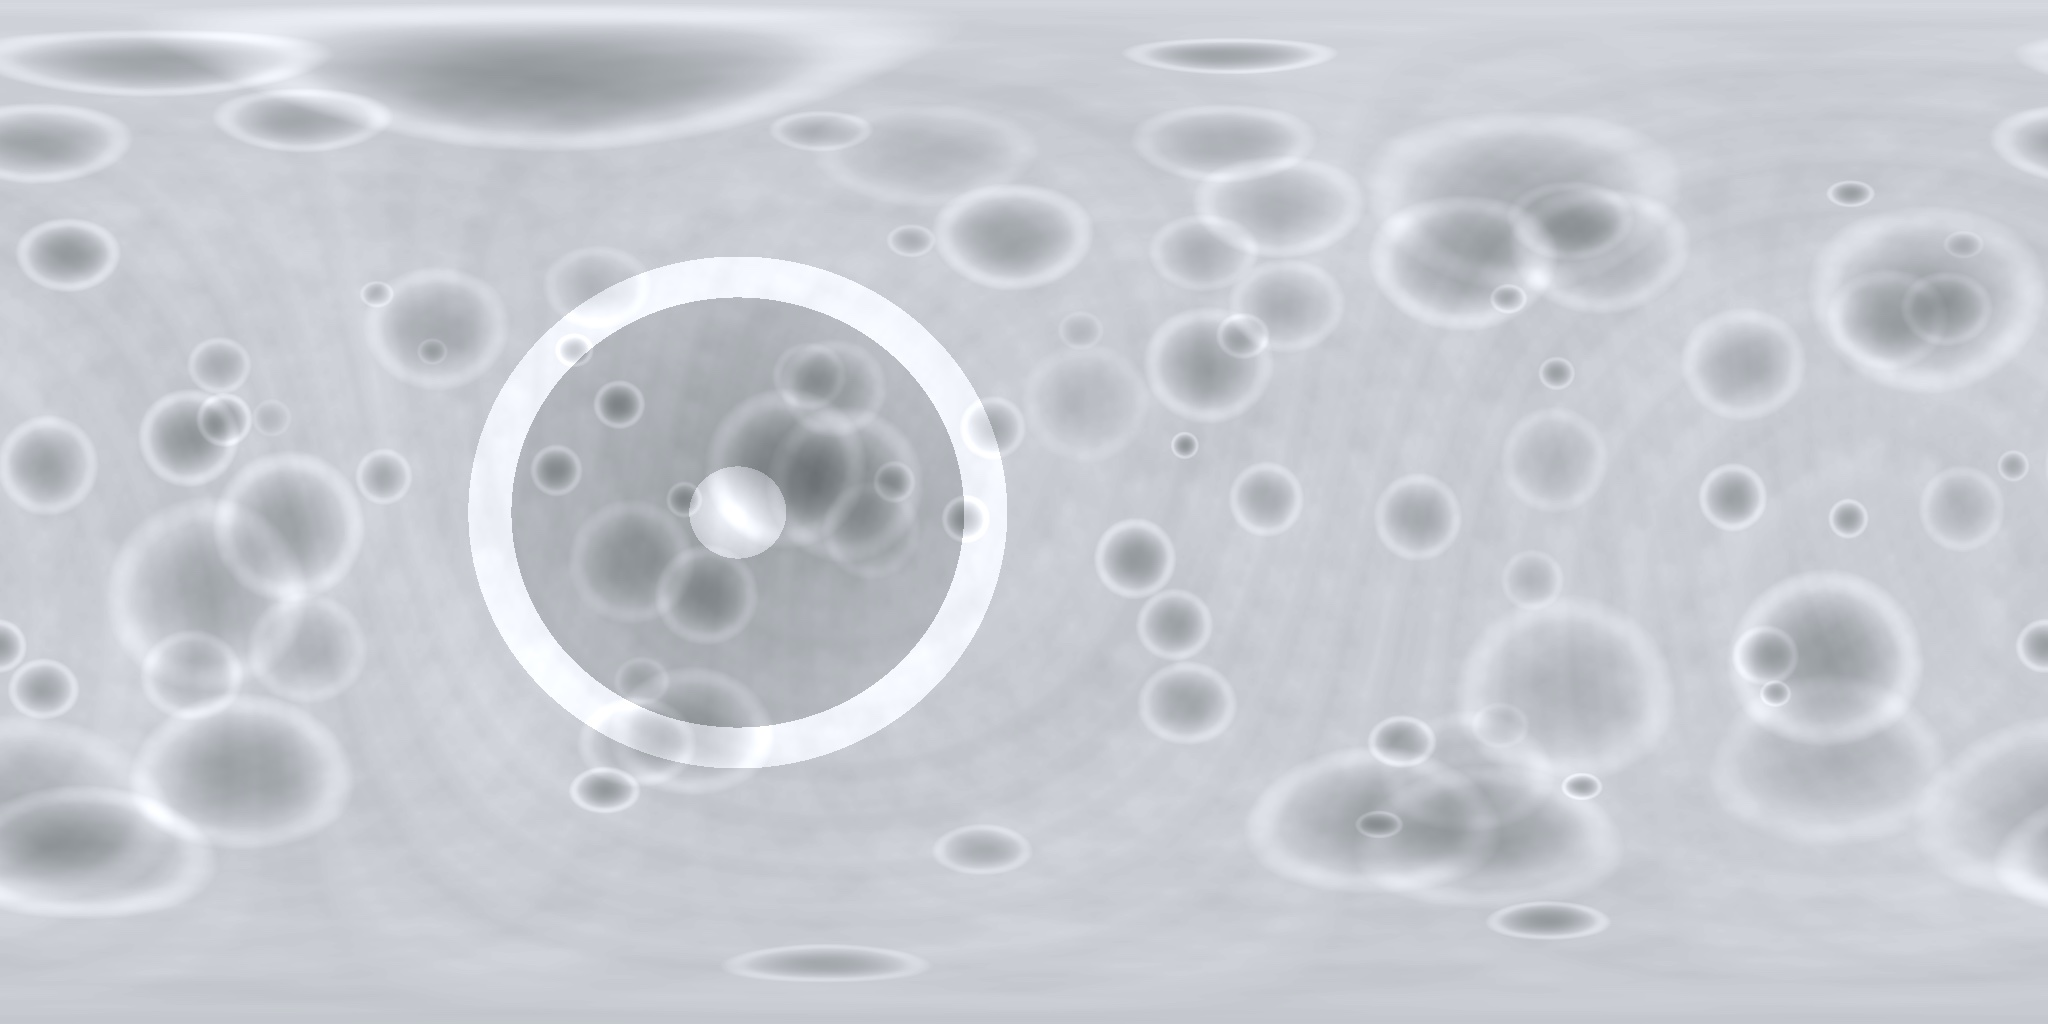
\includegraphics[width=\linewidth,height=4.4cm,keepaspectratio]{../public/textures/hd/mimas_cassini.jpg}\\[2pt]
{\scriptsize\itshape\color{orbitarMuted} Planiglob desfășurat: Harta satelitul înghețat Mimas și a uriașului crater Herschel, fotografiate de sonda NASA/ESA Cassini.}
\end{tabular}
\end{center}


\begin{tcolorbox}[orbitardata, title={\textbf{Repere esențiale: Mimas}}]
\small
\begin{itemize}[leftmargin=1.4em, itemsep=2pt, topsep=2pt]
  \item \textbf{Clasificare și orbită:} Satelit Natural (Lună) (orbitează în jurul: \textbf{Saturn}) \quad$\bullet$\quad \textbf{Distanță:} 9,582 UA ($\approx$ 1.433 milioane de kilometri)
  \item \textbf{Dimensiuni și masă:} rază medie 198,2 de kilometri \quad$\bullet$\quad masă: 6,30e-6 $\times M_\oplus$
  \item \textbf{Gravitație și regim termic:} 0,006 $\times g_\oplus$ (0,06 m/s$^2$) \quad$\bullet$\quad temperatură medie: -209 $^\circ$C (înclinarea axei: Nespecificată)
  \item \textbf{Ciclu orbital și rotație:} perioadă orbitală (an): 0,942 zile pământești \quad$\bullet$\quad rotație (zi): 22,61 ore (0,94 zile pământești)
  \item \textbf{Durata călătoriei de pe Pământ:} cu viteza luminii ($1c$): \emph{1 oră și 11 minute}; cu racheta ($50.000$ de kilometri pe oră): \emph{7 ani}; cu avionul ($900$ de kilometri pe oră): \emph{160 de ani}; cu mașina ($100$ de kilometri pe oră): \emph{1.450 de ani}.
  \item \textbf{Repere de scară și curiozitate:} Mimas este cel mai mic corp ceresc din Sistemul Solar care a reușit să devină rotund sub propria lui gravitație! Deși la exterior arată ca un glob înghețat și nemișcat, sub gheața lui Mimas se ascunde un ocean tânăr de apă lichidă!
\end{itemize}
\end{tcolorbox}

\subsubsection*{Prezentare generală și profil astrofizic}
Descoperită în 1789 de William Herschel, Mimas orbitează Saturn în doar 22 de ore și 36 de minute și curăță gravitațional celebra Diviziune Cassini dintre inelele A și B. Craterul Herschel are 139 de kilometri în diametru, ceea ce reprezintă o treime din diametrul întregului satelit! Mimas este o lună mică și înghețată a lui Saturn, celebră pentru craterul ei uriaș numit Herschel, care o face să arate exact ca o navă spațială din filme! Mimas este cel mai mic corp ceresc din Sistemul Solar care a reușit să devină rotund sub propria lui gravitație!

\subsubsection*{Alcătuirea fizică și structura internă}
Privind în profunzimea sa, alcătuirea fizică este organizată pe mai multe straturi și regiuni distincte, fiecare având un rol bine definit în evoluția și dinamica acestui obiect cosmic. În primul rând se remarcă \textbf{Nucleu stâncos}, înconjurat de un ocean global tânăr (format acum 5--15 milioane de ani), confirmat în 2024 din analiza librațiilor sondei Cassini. În strânsă legătură cu această componentă se află \textbf{Carapace groasă de gheață (20--30 de kilometri)}, atât de groasă încât nu prezintă gheizere la suprafață, spre deosebire de vecina Enceladus. În completarea acestui ansamblu întâlnim \textbf{Craterul Herschel}, ziduri de 5 kilometri înălțime și un piscul central de 6 kilometri, rezultat dintr-un impact la limita dezintegrării satelitului.

\subsubsection*{Observații astronomice și istoricul explorării}
Fotografiată de Voyager 1/2 și cartografiată la înaltă rezoluție de sonda Cassini între 2004 și 2017. Deși la exterior arată ca un glob înghețat și nemișcat, sub gheața lui Mimas se ascunde un ocean tânăr de apă lichidă!

\vspace{6pt}
\begin{tcolorbox}[orbitarquiz, title={\textbf{Întrebare de verificare \#15: Mimas}}]
\textbf{Ce formațiune geologică celebră ocupă o treime din diametrul satelitului Mimas?}
\begin{itemize}[leftmargin=2.2em, itemsep=2pt, topsep=4pt]
  \item[$\square$ \textbf{A.}] Craterul Herschel
  \item[$\square$ \textbf{B.}] Vulcanul Olympus Mons
  \item[$\square$ \textbf{C.}] Canionul Valles Marineris
  \item[$\square$ \textbf{D.}] Marea Tranquillitatis
\end{itemize}
\vspace{2pt}
{\footnotesize\color{orbitarMuted}\textbf{Răspuns corect:} \textbf{A} (Craterul Herschel). \emph{Craterul Herschel are 139 de kilometri lățime și un munte central înalt de 6 kilometri, dându-i lui Mimas aspectul său inconfundabil.}}
\end{tcolorbox}
\clearpage


\subsection{Enceladus}
\label{sec:body-enceladus}
\vspace{-4pt}
{\large\itshape\color{orbitarAccent} Luna albă ca zăpada a lui Saturn, cu gheizere cosmice}\\[4pt]


\begin{center}
\begin{tabular}{@{}m{0.44\textwidth}@{\hspace{0.03\textwidth}}m{0.51\textwidth}@{}}
\centering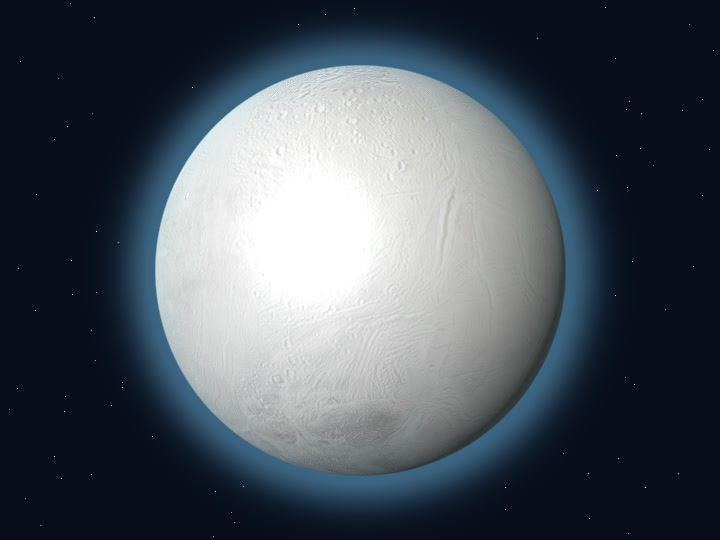
\includegraphics[width=\linewidth,height=4.4cm,keepaspectratio]{imagini/globuri/enceladus.jpg}\\[2pt]
{\scriptsize\itshape\color{orbitarMuted} Vedere 3D a corpului ceresc (\textbf{Enceladus})}
&
\centering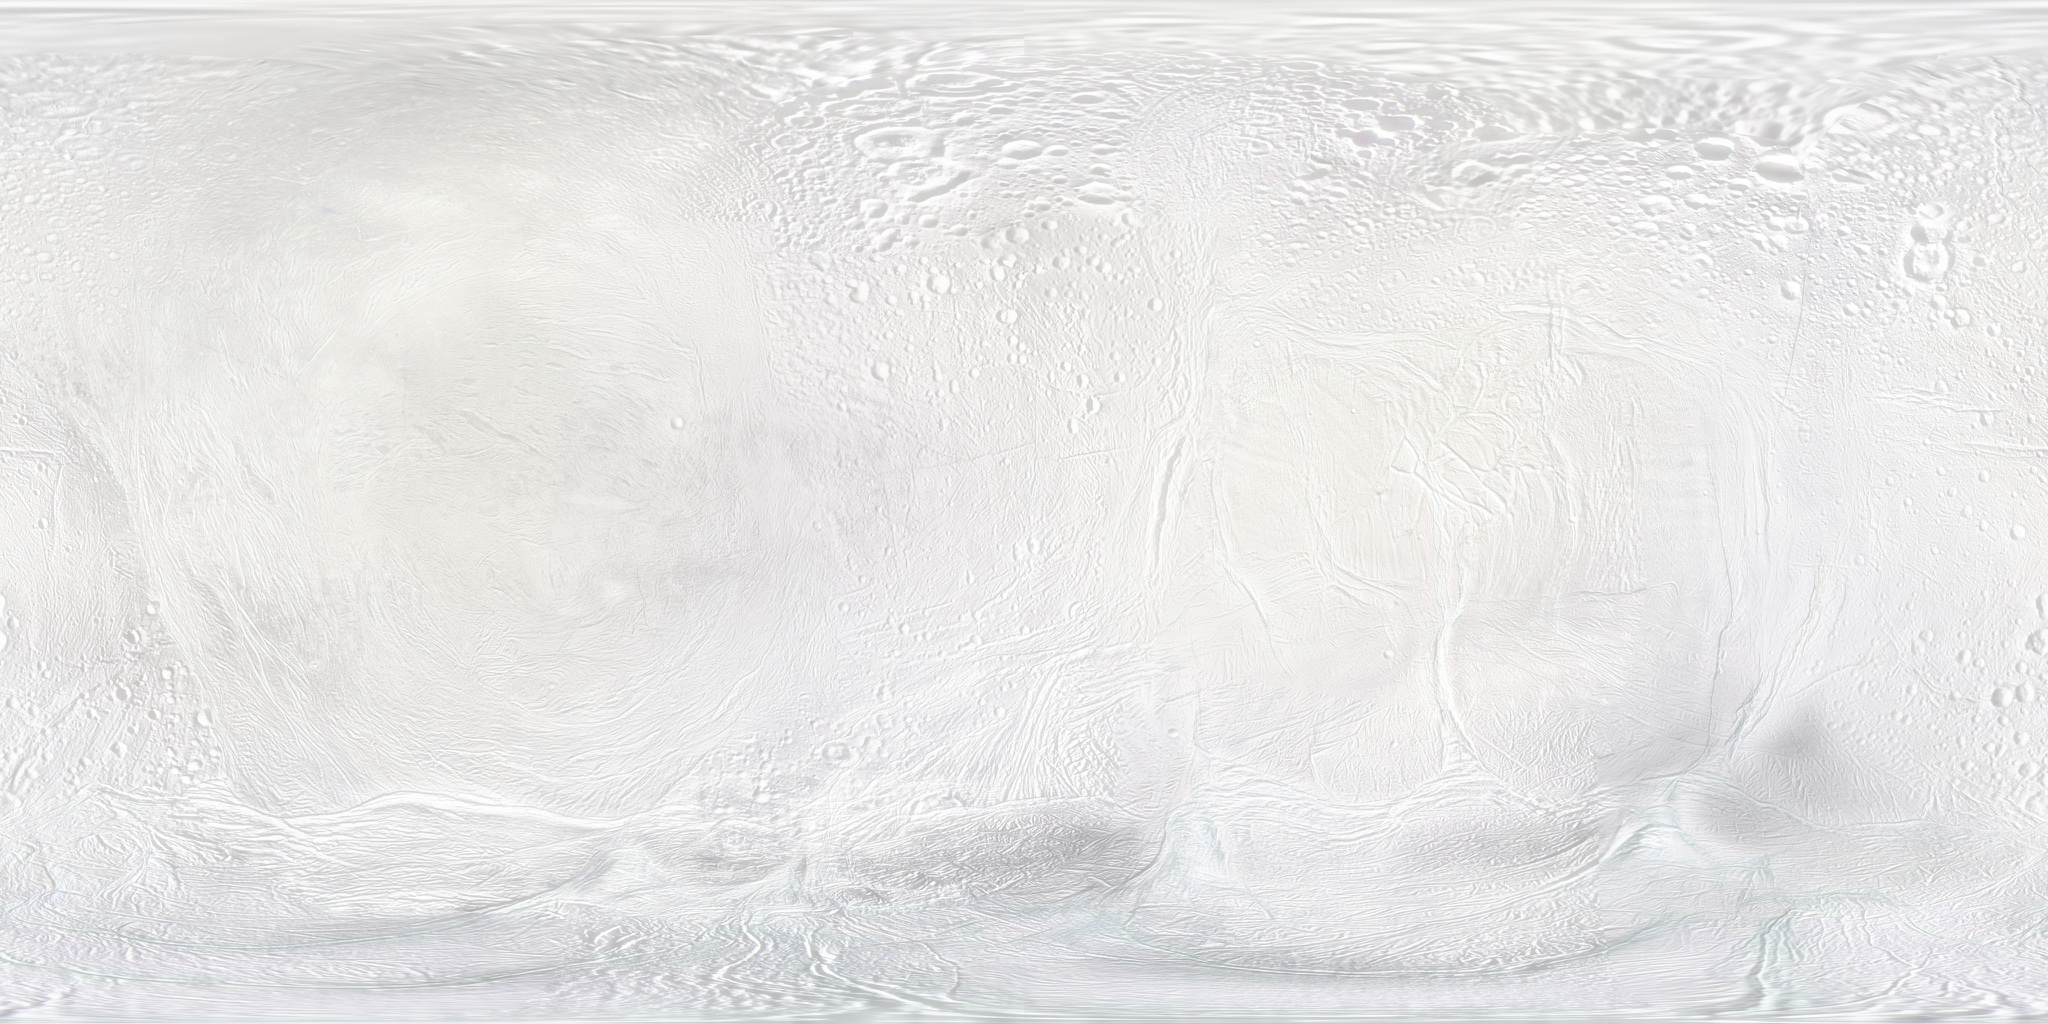
\includegraphics[width=\linewidth,height=4.4cm,keepaspectratio]{../public/textures/hd/enceladus_cassini.jpg}\\[2pt]
{\scriptsize\itshape\color{orbitarMuted} Planiglob desfășurat: Gheața pură a lunii Enceladus și fisurile \quotedblbase{}Dungi de Tigru\textquotedblright{} de la polul sudic (sonda NASA/ESA Cassini).}
\end{tabular}
\end{center}


\begin{tcolorbox}[orbitardata, title={\textbf{Repere esențiale: Enceladus}}]
\small
\begin{itemize}[leftmargin=1.4em, itemsep=2pt, topsep=2pt]
  \item \textbf{Clasificare și orbită:} Satelit Natural (Lună) (orbitează în jurul: \textbf{Saturn}) \quad$\bullet$\quad \textbf{Distanță:} 9,582 UA ($\approx$ 1.433 milioane de kilometri)
  \item \textbf{Dimensiuni și masă:} rază medie 252,1 de kilometri \quad$\bullet$\quad masă: 1,80e-5 $\times M_\oplus$
  \item \textbf{Gravitație și regim termic:} 0,011 $\times g_\oplus$ (0,11 m/s$^2$) \quad$\bullet$\quad temperatură medie: -198 $^\circ$C (înclinarea axei: Nespecificată)
  \item \textbf{Ciclu orbital și rotație:} perioadă orbitală (an): 1,37 zile pământești \quad$\bullet$\quad rotație (zi): 32,88 ore (1,37 zile pământești)
  \item \textbf{Durata călătoriei de pe Pământ:} cu viteza luminii ($1c$): \emph{1 oră și 11 minute}; cu racheta ($50.000$ de kilometri pe oră): \emph{7 ani}; cu avionul ($900$ de kilometri pe oră): \emph{160 de ani}; cu mașina ($100$ de kilometri pe oră): \emph{1.450 de ani}.
  \item \textbf{Repere de scară și curiozitate:} Enceladus este atât de mic încât ar încăpea cu ușurință deasupra României! Cristalele de gheață aruncate de gheizerele lui Enceladus formează unul dintre inelele lui Saturn (inelul E)!
\end{itemize}
\end{tcolorbox}

\subsubsection*{Prezentare generală și profil astrofizic}
Enceladus are cel mai ridicat albedo (reflectivitate) din Sistemul Solar (aproximativ 0,99). Sonda Cassini a zburat direct prin jeturile sale criovulcanice de la polul sud (\guillemotleft{}Dungile de Tigru\guillemotright{}), detectând apă sărată, molecule organice complexe, hidrogen molecular și silice hidrotermală. Enceladus este un bulgăre strălucitor de gheață proaspătă! La polul său sudic, gheizere uriașe aruncă apă și cristale de gheață direct în spațiu. Enceladus este atât de mic încât ar încăpea cu ușurință deasupra României!

\subsubsection*{Alcătuirea fizică și structura internă}
Privind în profunzimea sa, alcătuirea fizică este organizată pe mai multe straturi și regiuni distincte, fiecare având un rol bine definit în evoluția și dinamica acestui obiect cosmic. În primul rând se remarcă \textbf{Nucleu poros stâncos}, încălzit de mareele lui Saturn, generează izvoare hidrotermale pe fundul oceanului. În strânsă legătură cu această componentă se află \textbf{Ocean global subglaciar}, strat de apă lichidă de 30--40 de kilometri adâncime sub calota de gheață. În completarea acestui ansamblu întâlnim \textbf{Crustă de gheață pură și fisuri criovulcanice}, patru fracturi paralele calde la polul sudic prin care iese apa oceanică în vid.

\subsubsection*{Observații astronomice și istoricul explorării}
Descoperită de William Herschel în 1789; gheizerele sale au fost descoperite și analizate chimic de sonda Cassini în 2005--2015. Cristalele de gheață aruncate de gheizerele lui Enceladus formează unul dintre inelele lui Saturn (inelul E)!

\vspace{6pt}
\begin{tcolorbox}[orbitarquiz, title={\textbf{Întrebare de verificare \#16: Enceladus}}]
\textbf{Ce alimentează inelul E al planetei Saturn?}
\begin{itemize}[leftmargin=2.2em, itemsep=2pt, topsep=4pt]
  \item[$\square$ \textbf{A.}] Praf de pe Marte
  \item[$\square$ \textbf{B.}] Gheizerele de gheață și vapori de apă de la polul sud al lui Enceladus
  \item[$\square$ \textbf{C.}] Vântul solar
  \item[$\square$ \textbf{D.}] Asteroizii din Centura Kuiper
\end{itemize}
\vspace{2pt}
{\footnotesize\color{orbitarMuted}\textbf{Răspuns corect:} \textbf{B} (Gheizerele de gheață și vapori de apă de la polul sud al lui Enceladus). \emph{Jetul criovulcanic al lui Enceladus expulzează continuu granule de gheață care scapă de gravitația micului satelit și formează inelul E.}}
\end{tcolorbox}
\clearpage


\subsection{Tethys}
\label{sec:body-tethys}
\vspace{-4pt}
{\large\itshape\color{orbitarAccent} Luna de gheață pură a lui Saturn, cu craterul Odysseus și canionul Ithaca}\\[4pt]


\begin{center}
\begin{tabular}{@{}m{0.44\textwidth}@{\hspace{0.03\textwidth}}m{0.51\textwidth}@{}}
\centering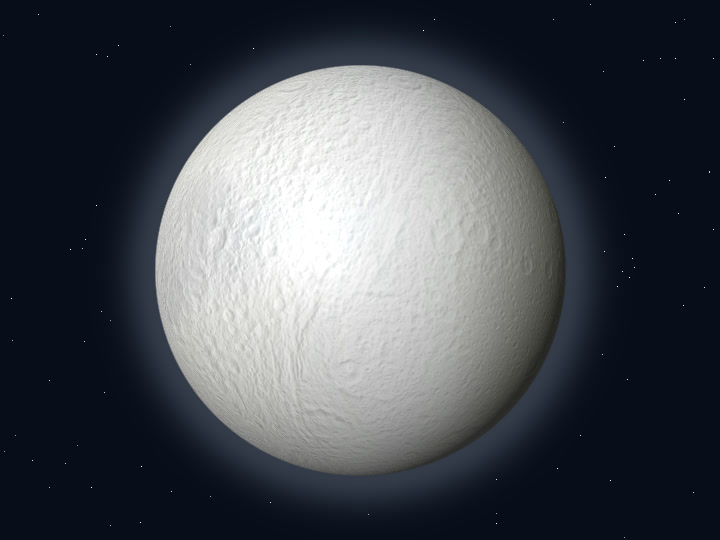
\includegraphics[width=\linewidth,height=4.4cm,keepaspectratio]{imagini/globuri/tethys.jpg}\\[2pt]
{\scriptsize\itshape\color{orbitarMuted} Vedere 3D a corpului ceresc (\textbf{Tethys})}
&
\centering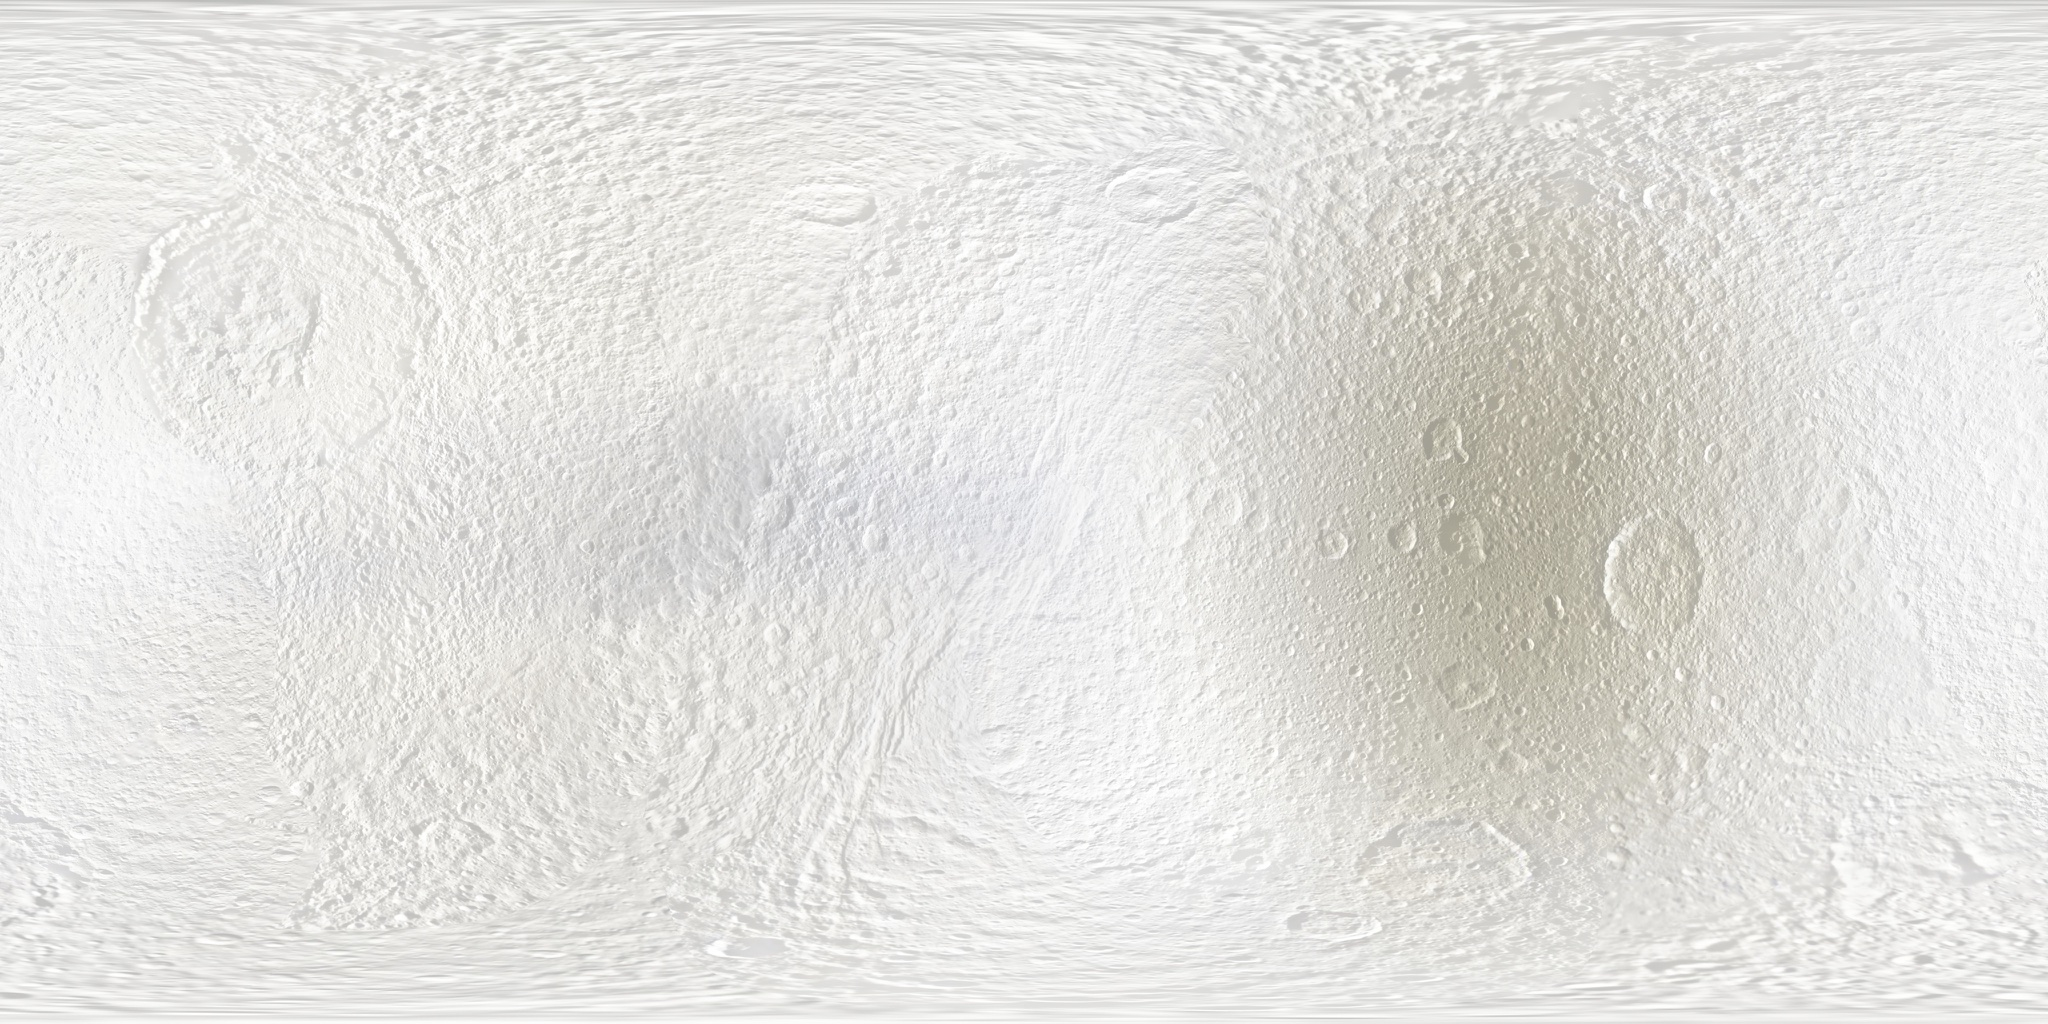
\includegraphics[width=\linewidth,height=4.4cm,keepaspectratio]{../public/textures/hd/tethys_cassini.jpg}\\[2pt]
{\scriptsize\itshape\color{orbitarMuted} Planiglob desfășurat: Harta globală a lunii înghețate Tethys, cu uriașul bazin de impact Odysseus și canionul Ithaca Chasma (NASA/ESA Cassini).}
\end{tabular}
\end{center}


\begin{tcolorbox}[orbitardata, title={\textbf{Repere esențiale: Tethys}}]
\small
\begin{itemize}[leftmargin=1.4em, itemsep=2pt, topsep=2pt]
  \item \textbf{Clasificare și orbită:} Satelit Natural (Lună) (orbitează în jurul: \textbf{Saturn}) \quad$\bullet$\quad \textbf{Distanță:} 9,582 UA ($\approx$ 1.433 milioane de kilometri)
  \item \textbf{Dimensiuni și masă:} rază medie 531,1 de kilometri \quad$\bullet$\quad masă: 1,03e-4 $\times M_\oplus$
  \item \textbf{Gravitație și regim termic:} 0,015 $\times g_\oplus$ (0,15 m/s$^2$) \quad$\bullet$\quad temperatură medie: -187 $^\circ$C (înclinarea axei: Nespecificată)
  \item \textbf{Ciclu orbital și rotație:} perioadă orbitală (an): 1,888 zile pământești \quad$\bullet$\quad rotație (zi): 45,31 ore (1,89 zile pământești)
  \item \textbf{Durata călătoriei de pe Pământ:} cu viteza luminii ($1c$): \emph{1 oră și 11 minute}; cu racheta ($50.000$ de kilometri pe oră): \emph{7 ani}; cu avionul ($900$ de kilometri pe oră): \emph{160 de ani}; cu mașina ($100$ de kilometri pe oră): \emph{1.450 de ani}.
  \item \textbf{Repere de scară și curiozitate:} Pentru că este făcută aproape doar din gheață, Tethys este mai ușoară decât apa, astfel că dacă ai găsi un ocean destul de mare, Tethys ar pluti pe el ca un cub de gheață! Canionul Ithaca Chasma de pe Tethys este lung de 2.000 de kilometri și încinge trei sferturi din întreaga lună ca o centură de gheață!
\end{itemize}
\end{tcolorbox}

\subsubsection*{Prezentare generală și profil astrofizic}
Descoperită de Giovanni Domenico Cassini în 1684, Tethys are cea mai scăzută densitate dintre toți sateliții majori din Sistemul Solar (0,984 g/cm$^3$), indicând că este compusă în proporție de peste 93\% din gheață de apă și mai puțin de 7\% rocă. Tethys este o lună mare și luminoasă a lui Saturn, formată aproape în întregime din gheață curată de apă! Pe ea se află un crater gigant numit Odysseus și o vale imensă de gheață. Pentru că este făcută aproape doar din gheață, Tethys este mai ușoară decât apa, astfel că dacă ai găsi un ocean destul de mare, Tethys ar pluti pe el ca un cub de gheață!

\subsubsection*{Alcătuirea fizică și structura internă}
Privind în profunzimea sa, alcătuirea fizică este organizată pe mai multe straturi și regiuni distincte, fiecare având un rol bine definit în evoluția și dinamica acestui obiect cosmic. În primul rând se remarcă \textbf{Interior omogen de gheață de apă}, densitatea de 0,984 g/cm$^3$ arată că fracțiunea stâncoasă este minimă. În strânsă legătură cu această componentă se află \textbf{Bazinul de impact Odysseus (445 de kilometri diametru)}, un crater colosal lat cât două cincimi din diametrul satelitului, ale cărui margini s-au aplatizat în timp prin relaxarea vâscoasă a gheții. În completarea acestui ansamblu întâlnim \textbf{Sistemul tectonic Ithaca Chasma}, o vale ramificată lată de 100 de kilometri, adâncă de 3--5 kilometri și lungă de 2.000 de kilometri, formată când oceanul intern străvechi al lui Tethys a înghețat și s-a dilatat.

\subsubsection*{Observații astronomice și istoricul explorării}
Fotografiată de Pioneer 11 și Voyager 1/2 și cartografiată la înaltă rezoluție de sonda Cassini în timpul survolului apropiat din septembrie 2005. Canionul Ithaca Chasma de pe Tethys este lung de 2.000 de kilometri și încinge trei sferturi din întreaga lună ca o centură de gheață!

\vspace{6pt}
\begin{tcolorbox}[orbitarquiz, title={\textbf{Întrebare de verificare \#17: Tethys}}]
\textbf{Din ce material este alcătuită în proporție de peste 93\% luna Tethys a lui Saturn?}
\begin{itemize}[leftmargin=2.2em, itemsep=2pt, topsep=4pt]
  \item[$\square$ \textbf{A.}] Din fier topit
  \item[$\square$ \textbf{B.}] Din gheață de apă aproape pură (având o densitate mai mică decât a apei lichide)
  \item[$\square$ \textbf{C.}] Din gaz metan
  \item[$\square$ \textbf{D.}] Din bazalt vulcanic negru
\end{itemize}
\vspace{2pt}
{\footnotesize\color{orbitarMuted}\textbf{Răspuns corect:} \textbf{B} (Din gheață de apă aproape pură (având o densitate mai mică decât a apei lichide)). \emph{Cu o densitate medie de 0,984 g/cm$^3$, Tethys este alcătuită aproape exclusiv din gheață de apă, reflectând puternic lumina Soarelui.}}
\end{tcolorbox}
\clearpage


\subsection{Dione}
\label{sec:body-dione}
\vspace{-4pt}
{\large\itshape\color{orbitarAccent} Luna înghețată a lui Saturn, brăzdată de faleze tectonice strălucitoare}\\[4pt]


\begin{center}
\begin{tabular}{@{}m{0.44\textwidth}@{\hspace{0.03\textwidth}}m{0.51\textwidth}@{}}
\centering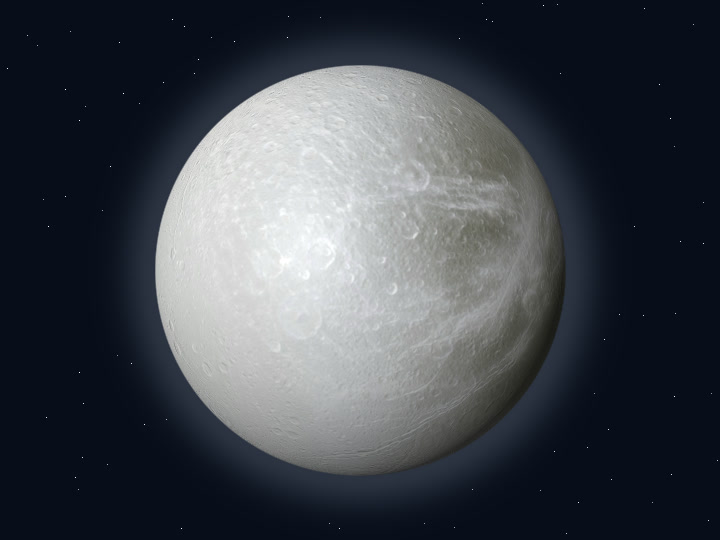
\includegraphics[width=\linewidth,height=4.4cm,keepaspectratio]{imagini/globuri/dione.jpg}\\[2pt]
{\scriptsize\itshape\color{orbitarMuted} Vedere 3D a corpului ceresc (\textbf{Dione})}
&
\centering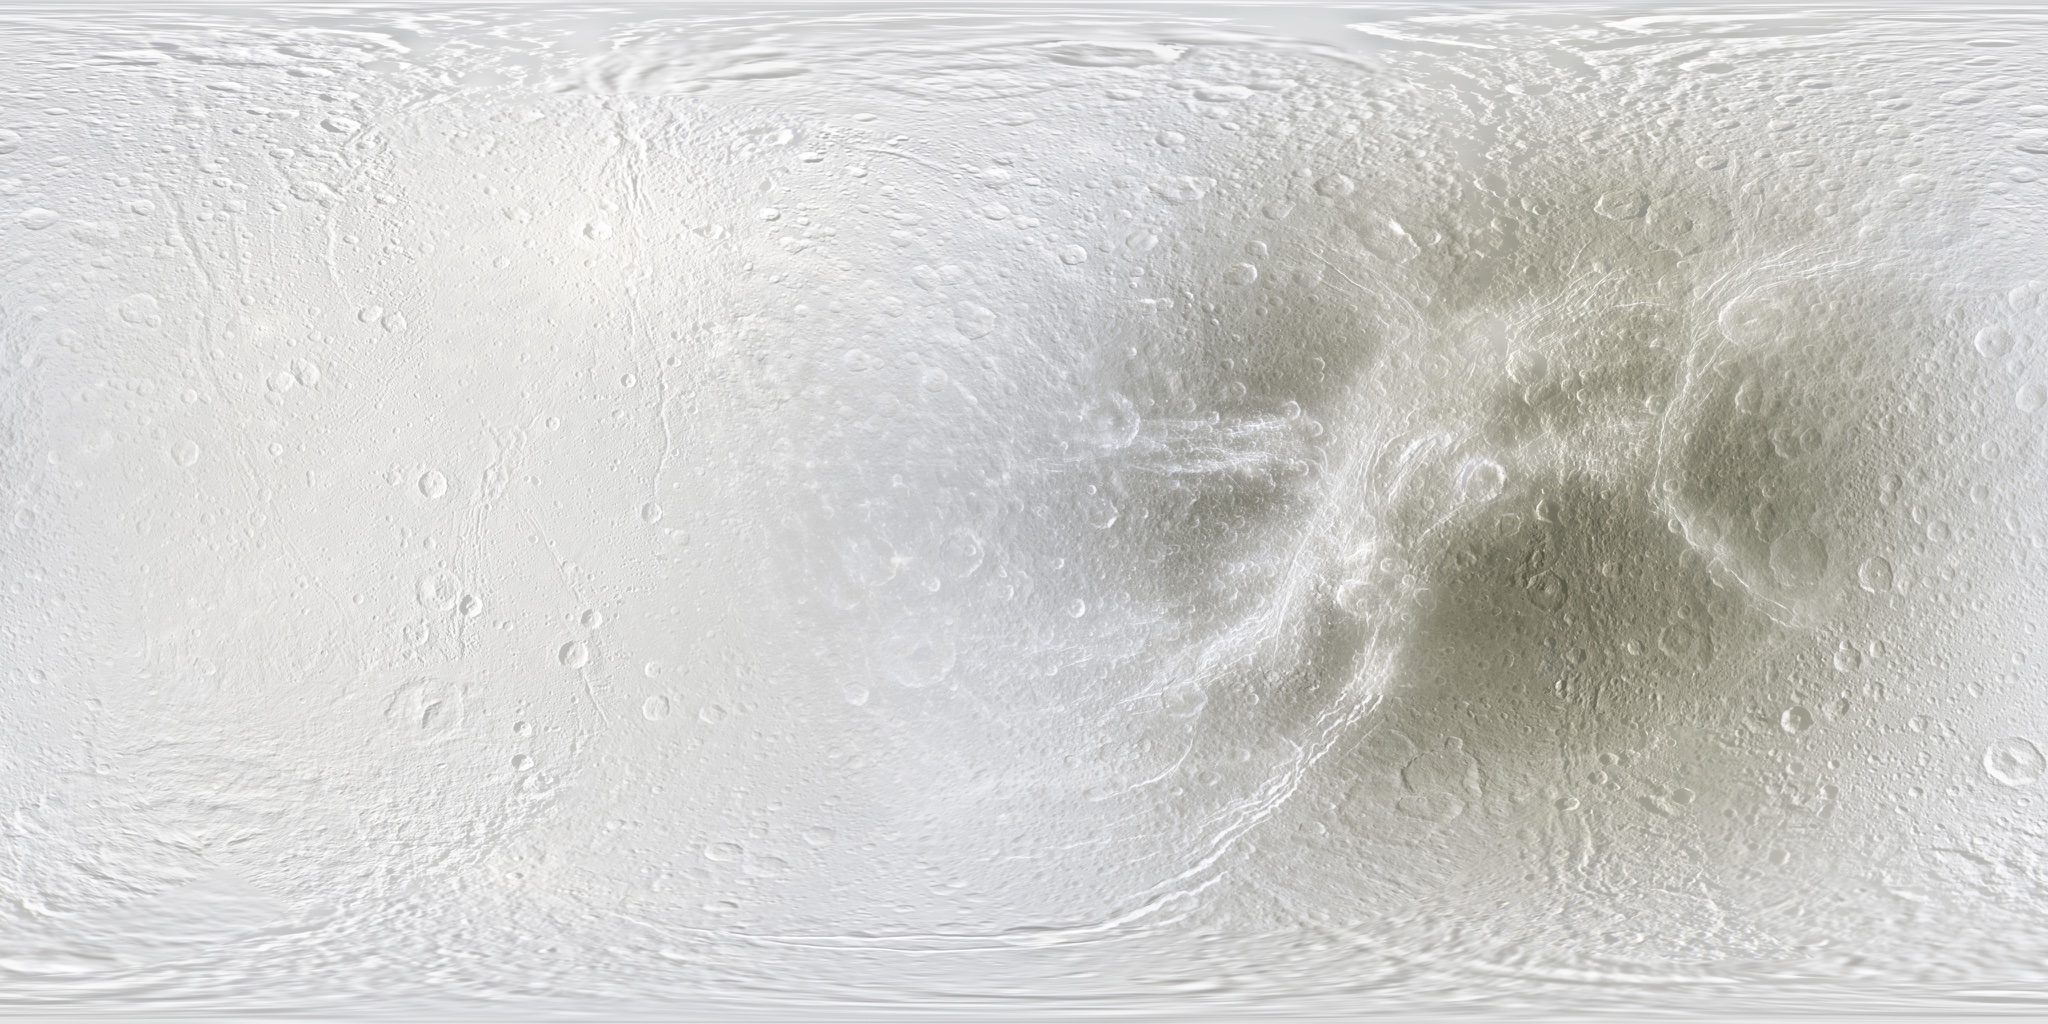
\includegraphics[width=\linewidth,height=4.4cm,keepaspectratio]{../public/textures/hd/dione_cassini.jpg}\\[2pt]
{\scriptsize\itshape\color{orbitarMuted} Planiglob desfășurat: Harta globală a lunii Dione și a falezelor luminoase de gheață Padua Chasmata (NASA/ESA Cassini).}
\end{tabular}
\end{center}


\begin{tcolorbox}[orbitardata, title={\textbf{Repere esențiale: Dione}}]
\small
\begin{itemize}[leftmargin=1.4em, itemsep=2pt, topsep=2pt]
  \item \textbf{Clasificare și orbită:} Satelit Natural (Lună) (orbitează în jurul: \textbf{Saturn}) \quad$\bullet$\quad \textbf{Distanță:} 9,582 UA ($\approx$ 1.433 milioane de kilometri)
  \item \textbf{Dimensiuni și masă:} rază medie 561,4 de kilometri \quad$\bullet$\quad masă: 1,83e-4 $\times M_\oplus$
  \item \textbf{Gravitație și regim termic:} 0,024 $\times g_\oplus$ (0,24 m/s$^2$) \quad$\bullet$\quad temperatură medie: -186 $^\circ$C (înclinarea axei: Nespecificată)
  \item \textbf{Ciclu orbital și rotație:} perioadă orbitală (an): 2,737 zile pământești \quad$\bullet$\quad rotație (zi): 65,69 ore (2,74 zile pământești)
  \item \textbf{Durata călătoriei de pe Pământ:} cu viteza luminii ($1c$): \emph{1 oră și 11 minute}; cu racheta ($50.000$ de kilometri pe oră): \emph{7 ani}; cu avionul ($900$ de kilometri pe oră): \emph{160 de ani}; cu mașina ($100$ de kilometri pe oră): \emph{1.450 de ani}.
  \item \textbf{Repere de scară și curiozitate:} Rețeaua de stânci luminoase de pe Dione arată din spațiu ca niște fire subțiri de beteală argintie așezate pe un glob înghețat! Două luni mici, Helene și Polydeuces, călătoresc pe exact aceeași orbită cu Dione, una în fața ei și cealaltă în urma ei!
\end{itemize}
\end{tcolorbox}

\subsubsection*{Prezentare generală și profil astrofizic}
Descoperită tot de Cassini în 1684, Dione are un diametru de 1.123 de kilometri și o densitate de 1,48 g/cm$^3$ (a treia cea mai mare dintre sateliții lui Saturn, după Titan și Enceladus), având un nucleu substanțial de silicați și posibil un ocean subteran sub o crustă groasă de gheață. Dione este a patra lună ca mărime a lui Saturn! Pe o parte a ei se văd dungi albe și sclipitoare care sunt, de fapt, stânci uriașe de gheață curată! Rețeaua de stânci luminoase de pe Dione arată din spațiu ca niște fire subțiri de beteală argintie așezate pe un glob înghețat!

\subsubsection*{Alcătuirea fizică și structura internă}
Privind în profunzimea sa, alcătuirea fizică este organizată pe mai multe straturi și regiuni distincte, fiecare având un rol bine definit în evoluția și dinamica acestui obiect cosmic. În primul rând se remarcă \textbf{Nucleu stâncos de silicați (aproximativ 46\% din masă)}, îi conferă o densitate semnificativ mai ridicată decât cea a vecinei Tethys. În strânsă legătură cu această componentă se află \textbf{Posibil ocean subglaciar profund}, indicat de datele gravimetrice și de topografie ale misiunii Cassini, situat la aproximativ 100 de kilometri sub suprafață. În completarea acestui ansamblu întâlnim \textbf{Falezele tectonice din Padua Chasmata}, fracturi de gheață luminoase înalte de sute de metri pe emisfera posterioară, cunoscute inițial drept \guillemotleft{}terenul vălurit\guillemotright{} (wispy terrain).

\subsubsection*{Observații astronomice și istoricul explorării}
Fotografiată de sondele Voyager și studiată în cinci survoluri apropiate de sonda Cassini între 2005 și 2015, care a detectat o exosferă extrem de rarefiată de ioni de oxigen. Două luni mici, Helene și Polydeuces, călătoresc pe exact aceeași orbită cu Dione, una în fața ei și cealaltă în urma ei!

\vspace{6pt}
\begin{tcolorbox}[orbitarquiz, title={\textbf{Întrebare de verificare \#18: Dione}}]
\textbf{Ce s-au dovedit a fi în realitate dungile albe luminoase (\guillemotleft{}wispy terrain\guillemotright{}) de pe satelitul Dione, fotografiate de aproape de sonda Cassini?}
\begin{itemize}[leftmargin=2.2em, itemsep=2pt, topsep=4pt]
  \item[$\square$ \textbf{A.}] Nori de ploaie
  \item[$\square$ \textbf{B.}] Faleze și canioane tectonice abrupte din gheață strălucitoare (precum Padua Chasmata)
  \item[$\square$ \textbf{C.}] Râuri de lavă
  \item[$\square$ \textbf{D.}] Dune de nisip galben
\end{itemize}
\vspace{2pt}
{\footnotesize\color{orbitarMuted}\textbf{Răspuns corect:} \textbf{B} (Faleze și canioane tectonice abrupte din gheață strălucitoare (precum Padua Chasmata)). \emph{Imaginile de înaltă rezoluție de la Cassini au arătat că dungile luminoase sunt pereți abrupți de falii tectonice unde gheața curată este expusă la suprafață.}}
\end{tcolorbox}
\clearpage


\subsection{Rhea}
\label{sec:body-rhea}
\vspace{-4pt}
{\large\itshape\color{orbitarAccent} A doua lună ca mărime a lui Saturn, un corp străvechi de gheață și stâncă}\\[4pt]


\begin{center}
\begin{tabular}{@{}m{0.44\textwidth}@{\hspace{0.03\textwidth}}m{0.51\textwidth}@{}}
\centering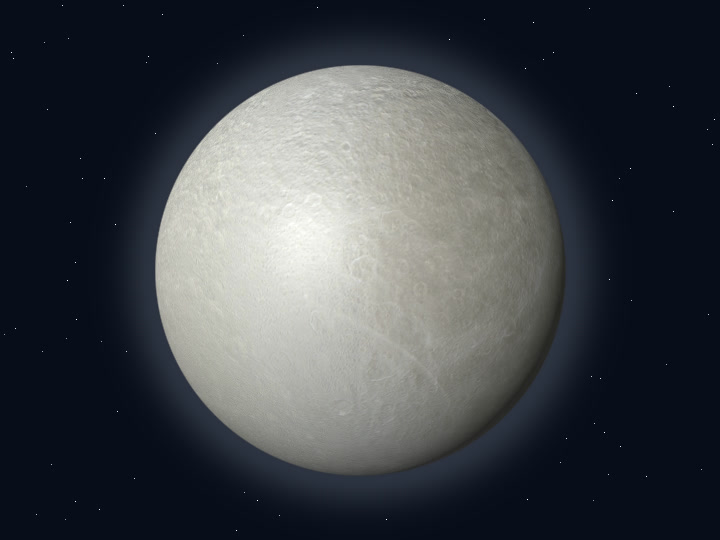
\includegraphics[width=\linewidth,height=4.4cm,keepaspectratio]{imagini/globuri/rhea.jpg}\\[2pt]
{\scriptsize\itshape\color{orbitarMuted} Vedere 3D a corpului ceresc (\textbf{Rhea})}
&
\centering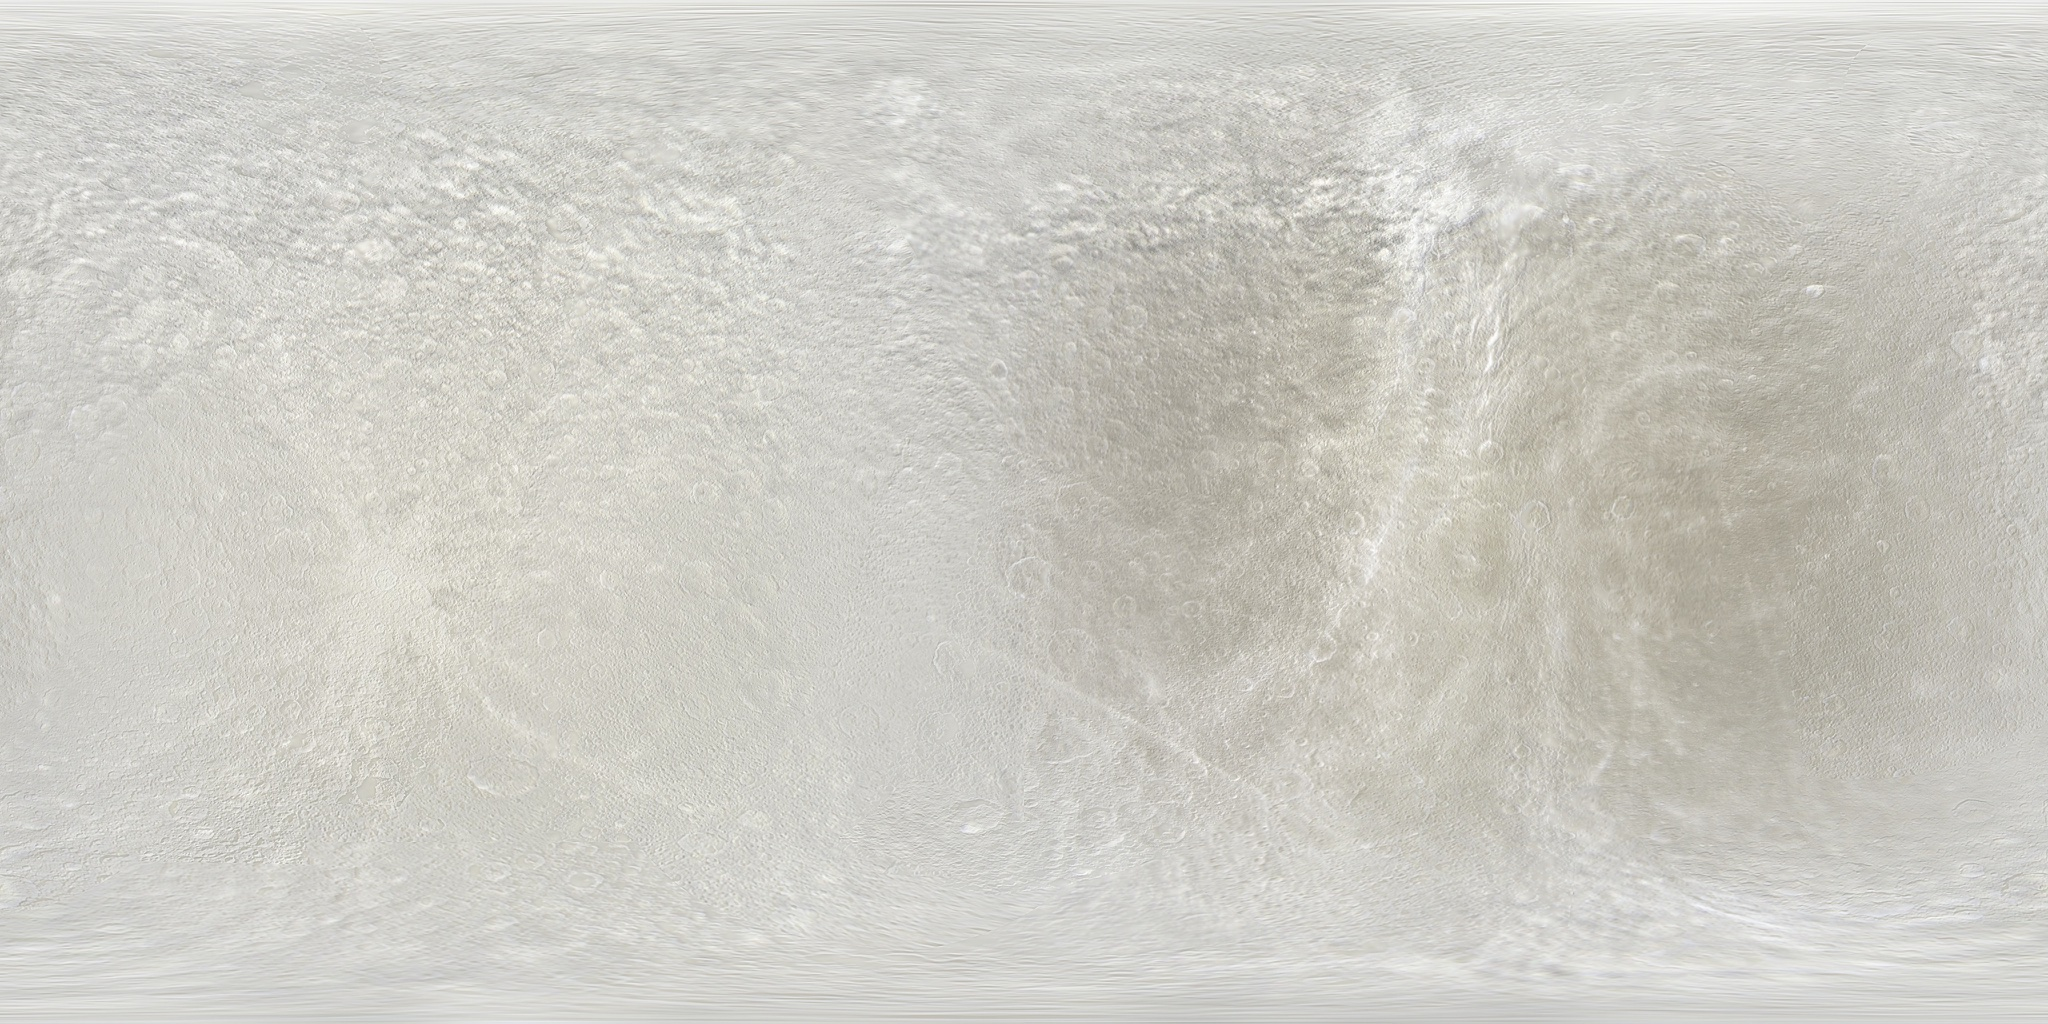
\includegraphics[width=\linewidth,height=4.4cm,keepaspectratio]{../public/textures/hd/rhea_cassini.jpg}\\[2pt]
{\scriptsize\itshape\color{orbitarMuted} Planiglob desfășurat: Suprafața intens craterizată a lunii Rhea, al doilea satelit ca mărime al lui Saturn (NASA/ESA Cassini).}
\end{tabular}
\end{center}


\begin{tcolorbox}[orbitardata, title={\textbf{Repere esențiale: Rhea}}]
\small
\begin{itemize}[leftmargin=1.4em, itemsep=2pt, topsep=2pt]
  \item \textbf{Clasificare și orbită:} Satelit Natural (Lună) (orbitează în jurul: \textbf{Saturn}) \quad$\bullet$\quad \textbf{Distanță:} 9,582 UA ($\approx$ 1.433 milioane de kilometri)
  \item \textbf{Dimensiuni și masă:} rază medie 763,8 de kilometri \quad$\bullet$\quad masă: 3,86e-4 $\times M_\oplus$
  \item \textbf{Gravitație și regim termic:} 0,027 $\times g_\oplus$ (0,26 m/s$^2$) \quad$\bullet$\quad temperatură medie: -197 $^\circ$C (înclinarea axei: Nespecificată)
  \item \textbf{Ciclu orbital și rotație:} perioadă orbitală (an): 4,518 zile pământești \quad$\bullet$\quad rotație (zi): 108,43 ore (4,52 zile pământești)
  \item \textbf{Durata călătoriei de pe Pământ:} cu viteza luminii ($1c$): \emph{1 oră și 11 minute}; cu racheta ($50.000$ de kilometri pe oră): \emph{7 ani}; cu avionul ($900$ de kilometri pe oră): \emph{160 de ani}; cu mașina ($100$ de kilometri pe oră): \emph{1.450 de ani}.
  \item \textbf{Repere de scară și curiozitate:} Rhea are un diametru de peste 1.500 de kilometri, fiind de aproape trei ori mai lată decât România! Sonda Cassini a descoperit în jurul lui Rhea o atmosferă extrem de subțire care conține oxigen și dioxid de carbon!
\end{itemize}
\end{tcolorbox}

\subsubsection*{Prezentare generală și profil astrofizic}
Descoperită în 1672 de Giovanni Domenico Cassini, Rhea este al nouălea satelit ca mărime din Sistemul Solar (diametru de 1.527,6 kilometri). Are o suprafață intens craterizată, împărțită între o emisferă anterioară luminoasă și o emisferă posterioară întunecată, brăzdată de canioane de gheață. Rhea este sora mai mare a lunilor de gheață ale lui Saturn și a doua lună ca mărime a planetei, imediat după uriașul Titan! Rhea are un diametru de peste 1.500 de kilometri, fiind de aproape trei ori mai lată decât România!

\subsubsection*{Alcătuirea fizică și structura internă}
Privind în profunzimea sa, alcătuirea fizică este organizată pe mai multe straturi și regiuni distincte, fiecare având un rol bine definit în evoluția și dinamica acestui obiect cosmic. În primul rând se remarcă \textbf{Interior slab diferențiat (75\% gheață, 25\% rocă)}, densitatea medie de 1,236 g/cm$^3$ indică un amestec de gheață de apă și roci silicatice. În strânsă legătură cu această componentă se află \textbf{Bazinele de impact Tirawa și Mamaldi}, două bazine străvechi uriașe (de 360 de kilometri și 480 de kilometri diametru) și craterul tânăr Inktomi cu raze strălucitoare de gheață pură. În completarea acestui ansamblu întâlnim \textbf{Exosferă fină de oxigen (O$_2$) și dioxid de carbon (CO$_2$)}, eliberată prin radioliza gheții de la suprafață sub acțiunea ionilor din magnetosfera lui Saturn.

\subsubsection*{Observații astronomice și istoricul explorării}
Fotografiată de sondele Voyager 1 și 2 și explorată îndeaproape de sonda Cassini (inclusiv un survol la doar 50 de kilometri altitudine în martie 2010). Sonda Cassini a descoperit în jurul lui Rhea o atmosferă extrem de subțire care conține oxigen și dioxid de carbon!

\vspace{6pt}
\begin{tcolorbox}[orbitarquiz, title={\textbf{Întrebare de verificare \#19: Rhea}}]
\textbf{Ce loc ocupă Rhea ca mărime între sateliții planetei Saturn?}
\begin{itemize}[leftmargin=2.2em, itemsep=2pt, topsep=4pt]
  \item[$\square$ \textbf{A.}] Este cel mai mic satelit
  \item[$\square$ \textbf{B.}] Este al doilea satelit ca mărime al lui Saturn, după Titan
  \item[$\square$ \textbf{C.}] Este mai mare decât Saturn
  \item[$\square$ \textbf{D.}] Este pe locul zece
\end{itemize}
\vspace{2pt}
{\footnotesize\color{orbitarMuted}\textbf{Răspuns corect:} \textbf{B} (Este al doilea satelit ca mărime al lui Saturn, după Titan). \emph{Cu o rază de 763,8 kilometri (diametru de 1.528 de kilometri), Rhea este a doua lună ca mărime a lui Saturn, fiind depășită doar de Titan.}}
\end{tcolorbox}
\clearpage


\subsection{Titan}
\label{sec:body-titan}
\vspace{-4pt}
{\large\itshape\color{orbitarAccent} Satelitul lui Saturn cu atmosferă densă și lacuri de metan}\\[4pt]


\begin{center}
\begin{tabular}{@{}m{0.44\textwidth}@{\hspace{0.03\textwidth}}m{0.51\textwidth}@{}}
\centering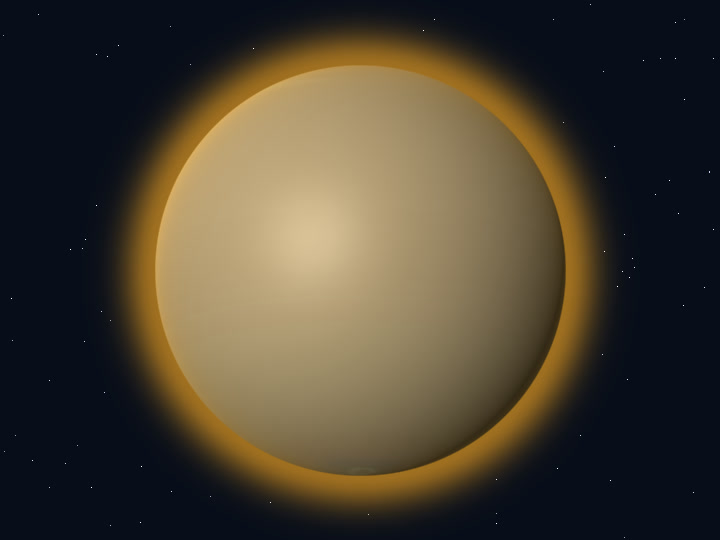
\includegraphics[width=\linewidth,height=4.4cm,keepaspectratio]{imagini/globuri/titan.jpg}\\[2pt]
{\scriptsize\itshape\color{orbitarMuted} Vedere 3D a corpului ceresc (\textbf{Titan})}
&
\centering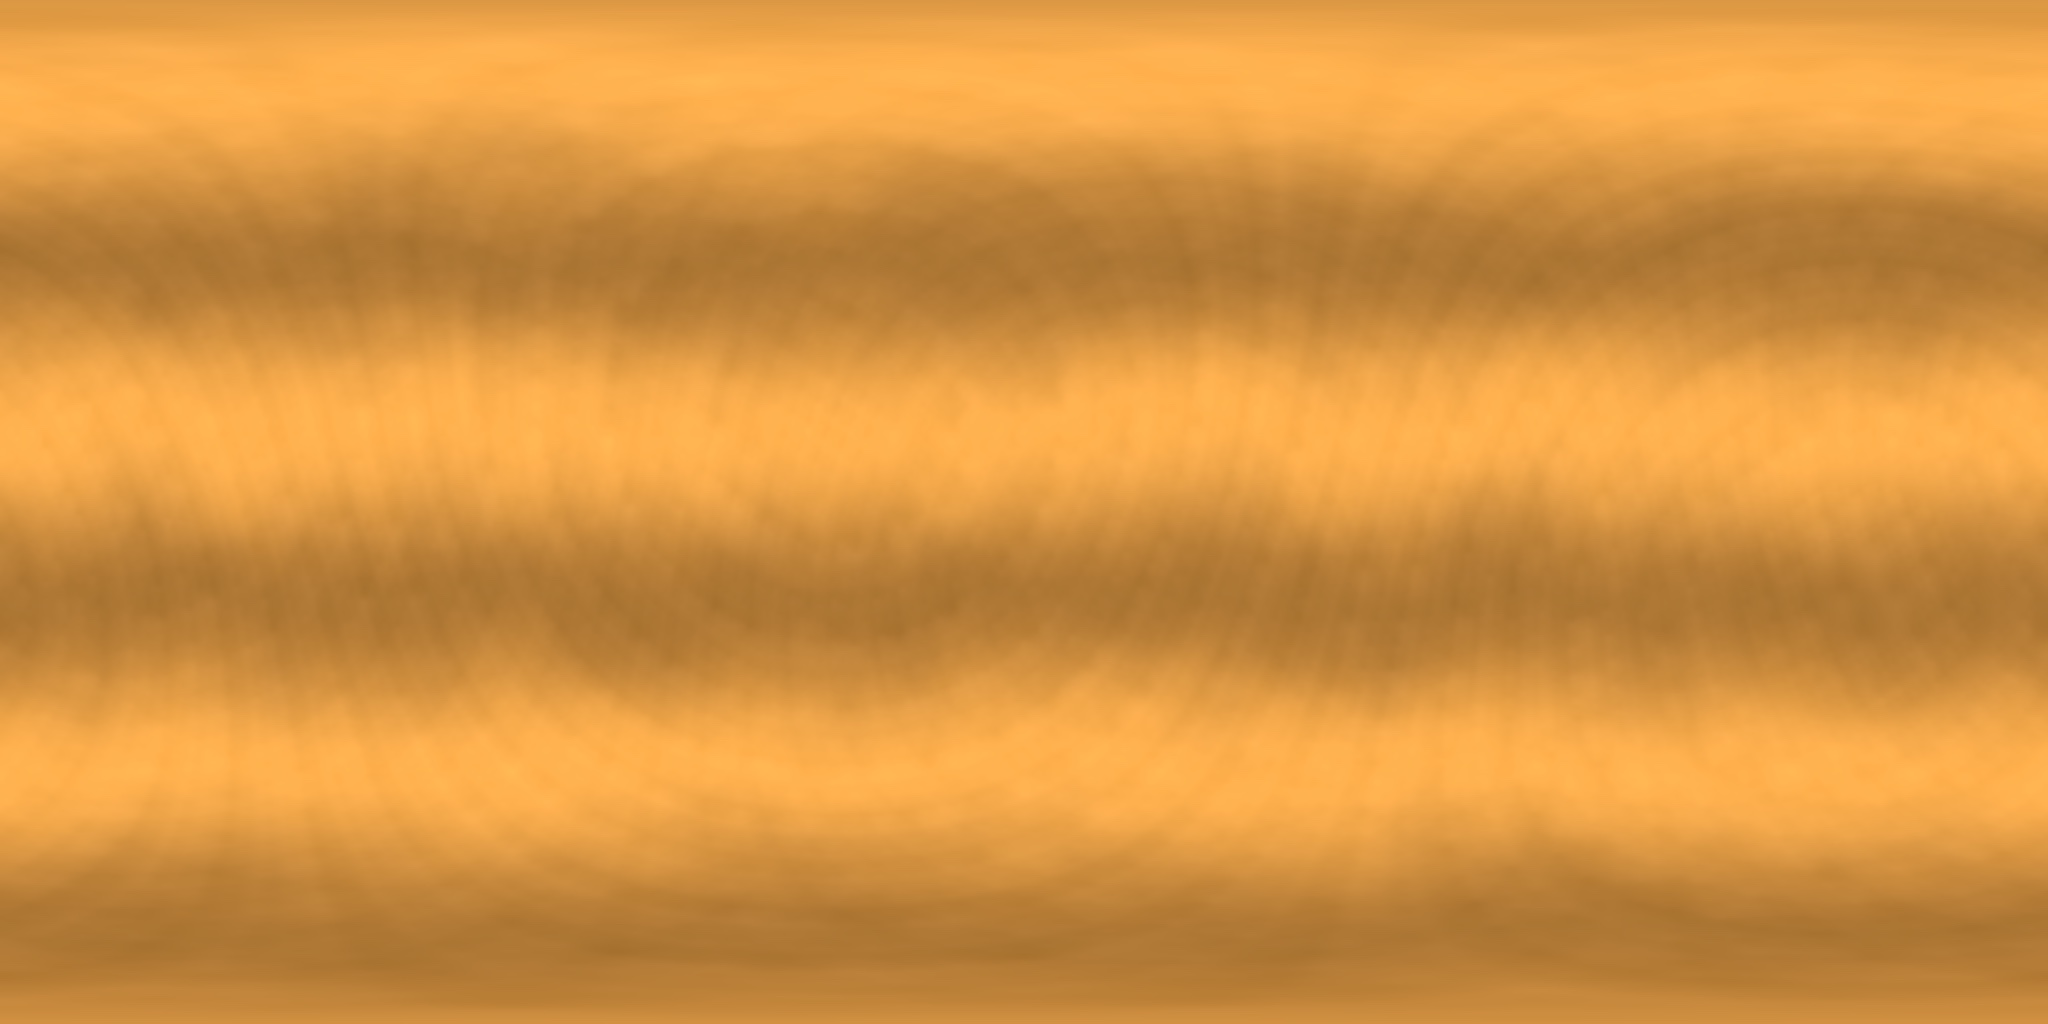
\includegraphics[width=\linewidth,height=4.4cm,keepaspectratio]{../public/textures/hd/titan_cassini.jpg}\\[2pt]
{\scriptsize\itshape\color{orbitarMuted} Planiglob desfășurat: Harta globală a lunii Titan obținută prin străpungerea ceții portocalii de azot și metan de către sonda Cassini.}
\end{tabular}
\end{center}


\begin{tcolorbox}[orbitardata, title={\textbf{Repere esențiale: Titan}}]
\small
\begin{itemize}[leftmargin=1.4em, itemsep=2pt, topsep=2pt]
  \item \textbf{Clasificare și orbită:} Satelit Natural (Lună) (orbitează în jurul: \textbf{Saturn}) \quad$\bullet$\quad \textbf{Distanță:} 9,582 UA ($\approx$ 1.433 milioane de kilometri)
  \item \textbf{Dimensiuni și masă:} rază medie 2.574,7 de kilometri \quad$\bullet$\quad masă: 0,022 $\times M_\oplus$
  \item \textbf{Gravitație și regim termic:} 0,138 $\times g_\oplus$ (1,35 m/s$^2$) \quad$\bullet$\quad temperatură medie: -179 $^\circ$C (înclinarea axei: Nespecificată)
  \item \textbf{Ciclu orbital și rotație:} perioadă orbitală (an): 15,945 zile pământești \quad$\bullet$\quad rotație (zi): 382,68 ore (15,95 zile pământești)
  \item \textbf{Durata călătoriei de pe Pământ:} cu viteza luminii ($1c$): \emph{1 oră și 11 minute}; cu racheta ($50.000$ de kilometri pe oră): \emph{7 ani}; cu avionul ($900$ de kilometri pe oră): \emph{160 de ani}; cu mașina ($100$ de kilometri pe oră): \emph{1.450 de ani}.
  \item \textbf{Repere de scară și curiozitate:} Pe Titan atmosfera e atât de deasă și gravitația atât de mică încât, dacă ți-ai pune aripi pe brațe, ai putea zbura dând din mâini ca o pasăre! Râurile și lacurile de pe Titan nu sunt din apă, ci din metan și etan lichid, la aproape -180 $^\circ$C!
\end{itemize}
\end{tcolorbox}

\subsubsection*{Prezentare generală și profil astrofizic}
Al doilea satelit ca mărime din Sistemul Solar (mai mare decât Mercur), Titan este singurul satelit cu o atmosferă densă (97\% azot, presiune de 1,45 ori mai mare decât pe Pământ) și singurul corp în afară de Pământ cu lichid stabil la suprafață. Titan este cea mai mare lună a lui Saturn și singura lună învelită într-o atmosferă groasă și portocalie, cu nori, ploi, râuri și mări! Pe Titan atmosfera e atât de deasă și gravitația atât de mică încât, dacă ți-ai pune aripi pe brațe, ai putea zbura dând din mâini ca o pasăre!

\subsubsection*{Alcătuirea fizică și structura internă}
Privind în profunzimea sa, alcătuirea fizică este organizată pe mai multe straturi și regiuni distincte, fiecare având un rol bine definit în evoluția și dinamica acestui obiect cosmic. În primul rând se remarcă \textbf{Nucleu de silicați hidratati}, cu o rază de aproximativ 2.000 de kilometri în centrul satelitului. În strânsă legătură cu această componentă se află \textbf{Ocean subteran de apă și amoniac}, situat sub o crustă de gheață de apă dură ca roca. În completarea acestui ansamblu întâlnim \textbf{Suprafață cu ciclu al metanului și atmosferă de azot}, mări de hidrocarburi (Kraken Mare, Ligeia Mare), dune organice și ceață fotochimică (toline).

\subsubsection*{Observații astronomice și istoricul explorării}
Sonda europeană Huygens a asolizat pe Titan în ianuarie 2005 (cea mai îndepărtată asolizare din istorie); NASA pregătește drona nucleară Dragonfly. Râurile și lacurile de pe Titan nu sunt din apă, ci din metan și etan lichid, la aproape -180 $^\circ$C!

\vspace{6pt}
\begin{tcolorbox}[orbitarquiz, title={\textbf{Întrebare de verificare \#20: Titan}}]
\textbf{Din ce sunt formate lacurile și mările de la suprafața lui Titan?}
\begin{itemize}[leftmargin=2.2em, itemsep=2pt, topsep=4pt]
  \item[$\square$ \textbf{A.}] Din apă caldă
  \item[$\square$ \textbf{B.}] Din metan și etan lichid
  \item[$\square$ \textbf{C.}] Din lavă topită
  \item[$\square$ \textbf{D.}] Din mercur lichid
\end{itemize}
\vspace{2pt}
{\footnotesize\color{orbitarMuted}\textbf{Răspuns corect:} \textbf{B} (Din metan și etan lichid). \emph{La temperatura de -179 $^\circ$C de pe Titan, apa este tare ca piatra, iar metanul și etanul formează nori, ploi, râuri și mări.}}
\end{tcolorbox}
\clearpage


\subsection{Hyperion}
\label{sec:body-hyperion}
\vspace{-4pt}
{\large\itshape\color{orbitarAccent} Luna-burete a lui Saturn, cu cratere în formă de fagure și rotație haotică}\\[4pt]


\begin{center}
\begin{tabular}{@{}m{0.44\textwidth}@{\hspace{0.03\textwidth}}m{0.51\textwidth}@{}}
\centering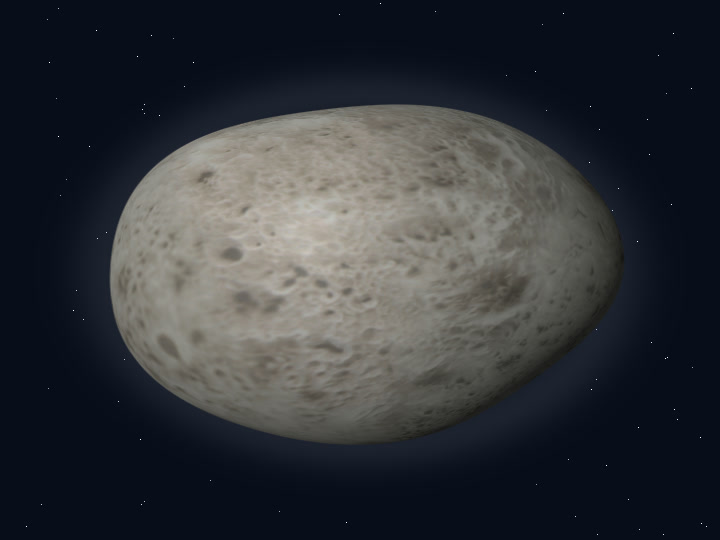
\includegraphics[width=\linewidth,height=4.4cm,keepaspectratio]{imagini/globuri/hyperion.jpg}\\[2pt]
{\scriptsize\itshape\color{orbitarMuted} Vedere 3D a corpului ceresc (\textbf{Hyperion})}
&
\centering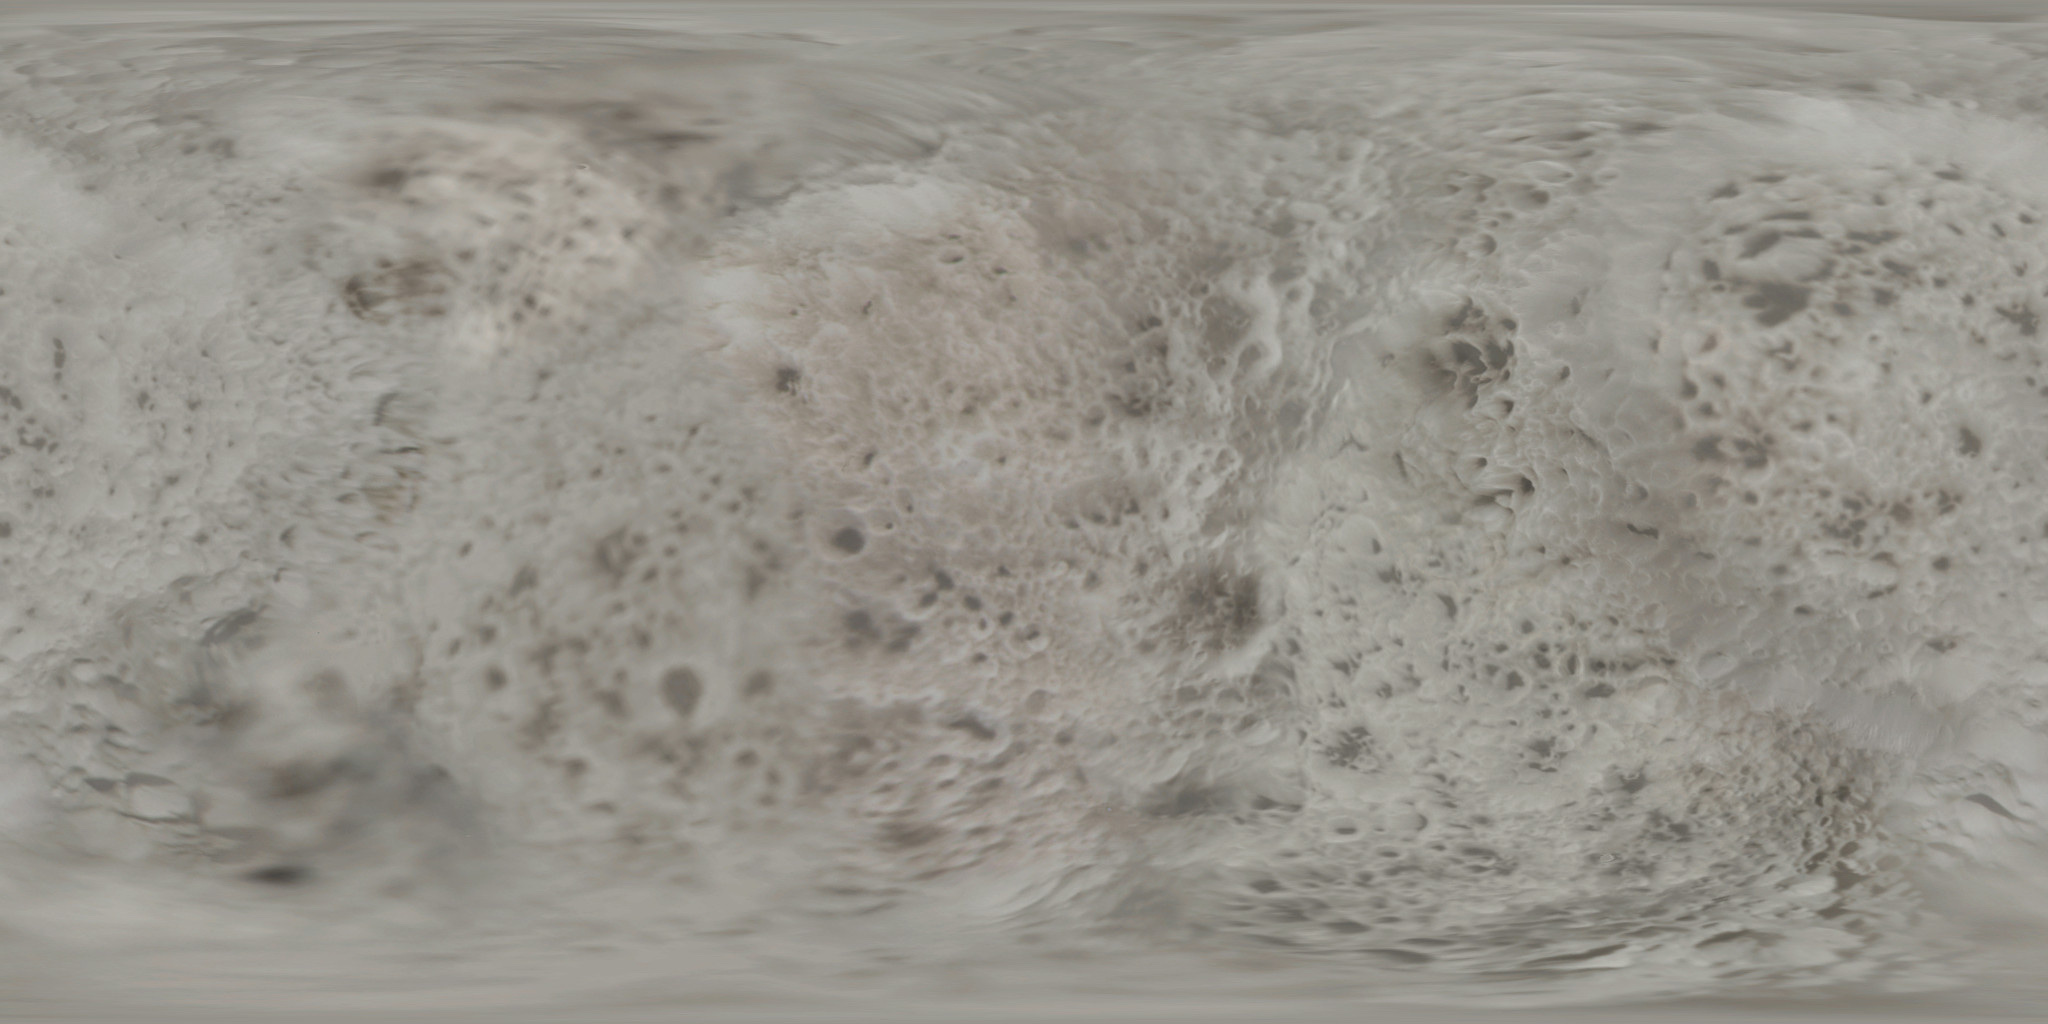
\includegraphics[width=\linewidth,height=4.4cm,keepaspectratio]{../public/textures/hd/hyperion_cassini.jpg}\\[2pt]
{\scriptsize\itshape\color{orbitarMuted} Planiglob desfășurat: Aspectul poros, de \quotedblbase{}burete cosmic\textquotedblright{} ciuruit de cratere adânci, al satelitului cu rotație haotică Hyperion (NASA/ESA Cassini).}
\end{tabular}
\end{center}


\begin{tcolorbox}[orbitardata, title={\textbf{Repere esențiale: Hyperion}}]
\small
\begin{itemize}[leftmargin=1.4em, itemsep=2pt, topsep=2pt]
  \item \textbf{Clasificare și orbită:} Satelit Natural (Lună) (orbitează în jurul: \textbf{Saturn}) \quad$\bullet$\quad \textbf{Distanță:} 9,582 UA ($\approx$ 1.433 milioane de kilometri)
  \item \textbf{Dimensiuni și masă:} rază medie 135 de kilometri \quad$\bullet$\quad masă: 9,40e-7 $\times M_\oplus$
  \item \textbf{Gravitație și regim termic:} 0,002 $\times g_\oplus$ (0,02 m/s$^2$) \quad$\bullet$\quad temperatură medie: -180 $^\circ$C (înclinarea axei: Nespecificată)
  \item \textbf{Ciclu orbital și rotație:} perioadă orbitală (an): 21,276 zile pământești \quad$\bullet$\quad rotație (zi): 120,00 ore (5,00 zile pământești)
  \item \textbf{Durata călătoriei de pe Pământ:} cu viteza luminii ($1c$): \emph{1 oră și 11 minute}; cu racheta ($50.000$ de kilometri pe oră): \emph{7 ani}; cu avionul ($900$ de kilometri pe oră): \emph{160 de ani}; cu mașina ($100$ de kilometri pe oră): \emph{1.450 de ani}.
  \item \textbf{Repere de scară și curiozitate:} În timp ce alte luni se rotesc ordonat, Hyperion se rostogolește haotic prin spațiu, așa că pe el nu ai ști niciodată din ce direcție va răsări Saturn mâine! Hyperion este mai mult de 40\% gol pe dinăuntru, ca o spumă înghețată de apă și praf cosmic!
\end{itemize}
\end{tcolorbox}

\subsubsection*{Prezentare generală și profil astrofizic}
Descoperită în 1848 de William și George Bond și independent de William Lassell, Hyperion (360 $\times$ 266 $\times$ 205 kilometri) este unul dintre cele mai mari corpuri neregulate din Sistemul Solar și primul satelit la care s-a descoperit o rotație complet haotică, cauzată de rezonanța orbitală 4:3 cu Titan. Hyperion este cea mai ciudată lună a lui Saturn: nu este rotundă și este atât de plină de găuri adânci încât arată exact ca un burete de mare înghețat! În timp ce alte luni se rotesc ordonat, Hyperion se rostogolește haotic prin spațiu, așa că pe el nu ai ști niciodată din ce direcție va răsări Saturn mâine!

\subsubsection*{Alcătuirea fizică și structura internă}
Privind în profunzimea sa, alcătuirea fizică este organizată pe mai multe straturi și regiuni distincte, fiecare având un rol bine definit în evoluția și dinamica acestui obiect cosmic. În primul rând se remarcă \textbf{Structură ultra-poroasă (\guillemotleft{}burete cosmic\guillemotright{})}, densitate medie de numai 0,544 g/cm$^3$ (jumătate din cea a apei), cu o porozitate internă de peste 40\%. În strânsă legătură cu această componentă se află \textbf{Cratere adânci în formă de fagure}, din cauza porozității mari, meteoriții comprimă gheața la impact fără a arunca mult material în jur, lăsând pereți abrupți și strălucitori. În completarea acestui ansamblu întâlnim \textbf{Hidrocarburi întunecate pe fundul craterelor}, unde praful bogat în compuși de carbon și cianoacetilenă se adună pe fundul craterelor și absoarbe lumina solară, sublimând gheața.

\subsubsection*{Observații astronomice și istoricul explorării}
Fotografiată în detaliu uimitor de sonda Cassini la 26 septembrie 2005, în timpul unui survol apropiat la numai 500 de kilometri distanță. Hyperion este mai mult de 40\% gol pe dinăuntru, ca o spumă înghețată de apă și praf cosmic!

\vspace{6pt}
\begin{tcolorbox}[orbitarquiz, title={\textbf{Întrebare de verificare \#21: Hyperion}}]
\textbf{De ce seamănă satelitul Hyperion al lui Saturn cu un burete sau un fagure înghețat?}
\begin{itemize}[leftmargin=2.2em, itemsep=2pt, topsep=4pt]
  \item[$\square$ \textbf{A.}] Are o porozitate internă de peste 40\%, iar impacturile comprimă gheața în cratere adânci cu margini ascuțite
  \item[$\square$ \textbf{B.}] A fost săpat de vulcani
  \item[$\square$ \textbf{C.}] Este făcut din fier greu
  \item[$\square$ \textbf{D.}] Are oceane calde la suprafață
\end{itemize}
\vspace{2pt}
{\footnotesize\color{orbitarMuted}\textbf{Răspuns corect:} \textbf{A} (Are o porozitate internă de peste 40\%, iar impacturile comprimă gheața în cratere adânci cu margini ascuțite). \emph{Cu o densitate de doar 0,54 g/cm$^3$, Hyperion este extrem de poros, astfel încât impacturile meteoritice creează cavități adânci prin compresie, fără a le șterge pe cele vecine.}}
\end{tcolorbox}
\clearpage


\subsection{Iapetus}
\label{sec:body-iapetus}
\vspace{-4pt}
{\large\itshape\color{orbitarAccent} Luna bicoloră \guillemotleft{}Yin-Yang\guillemotright{} a lui Saturn, cu formă de nucă}\\[4pt]


\begin{center}
\begin{tabular}{@{}m{0.44\textwidth}@{\hspace{0.03\textwidth}}m{0.51\textwidth}@{}}
\centering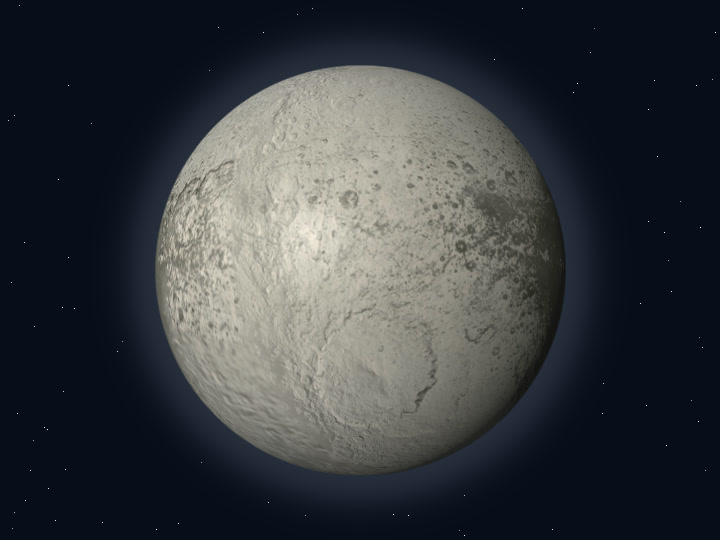
\includegraphics[width=\linewidth,height=4.4cm,keepaspectratio]{imagini/globuri/iapetus.jpg}\\[2pt]
{\scriptsize\itshape\color{orbitarMuted} Vedere 3D a corpului ceresc (\textbf{Iapetus})}
&
\centering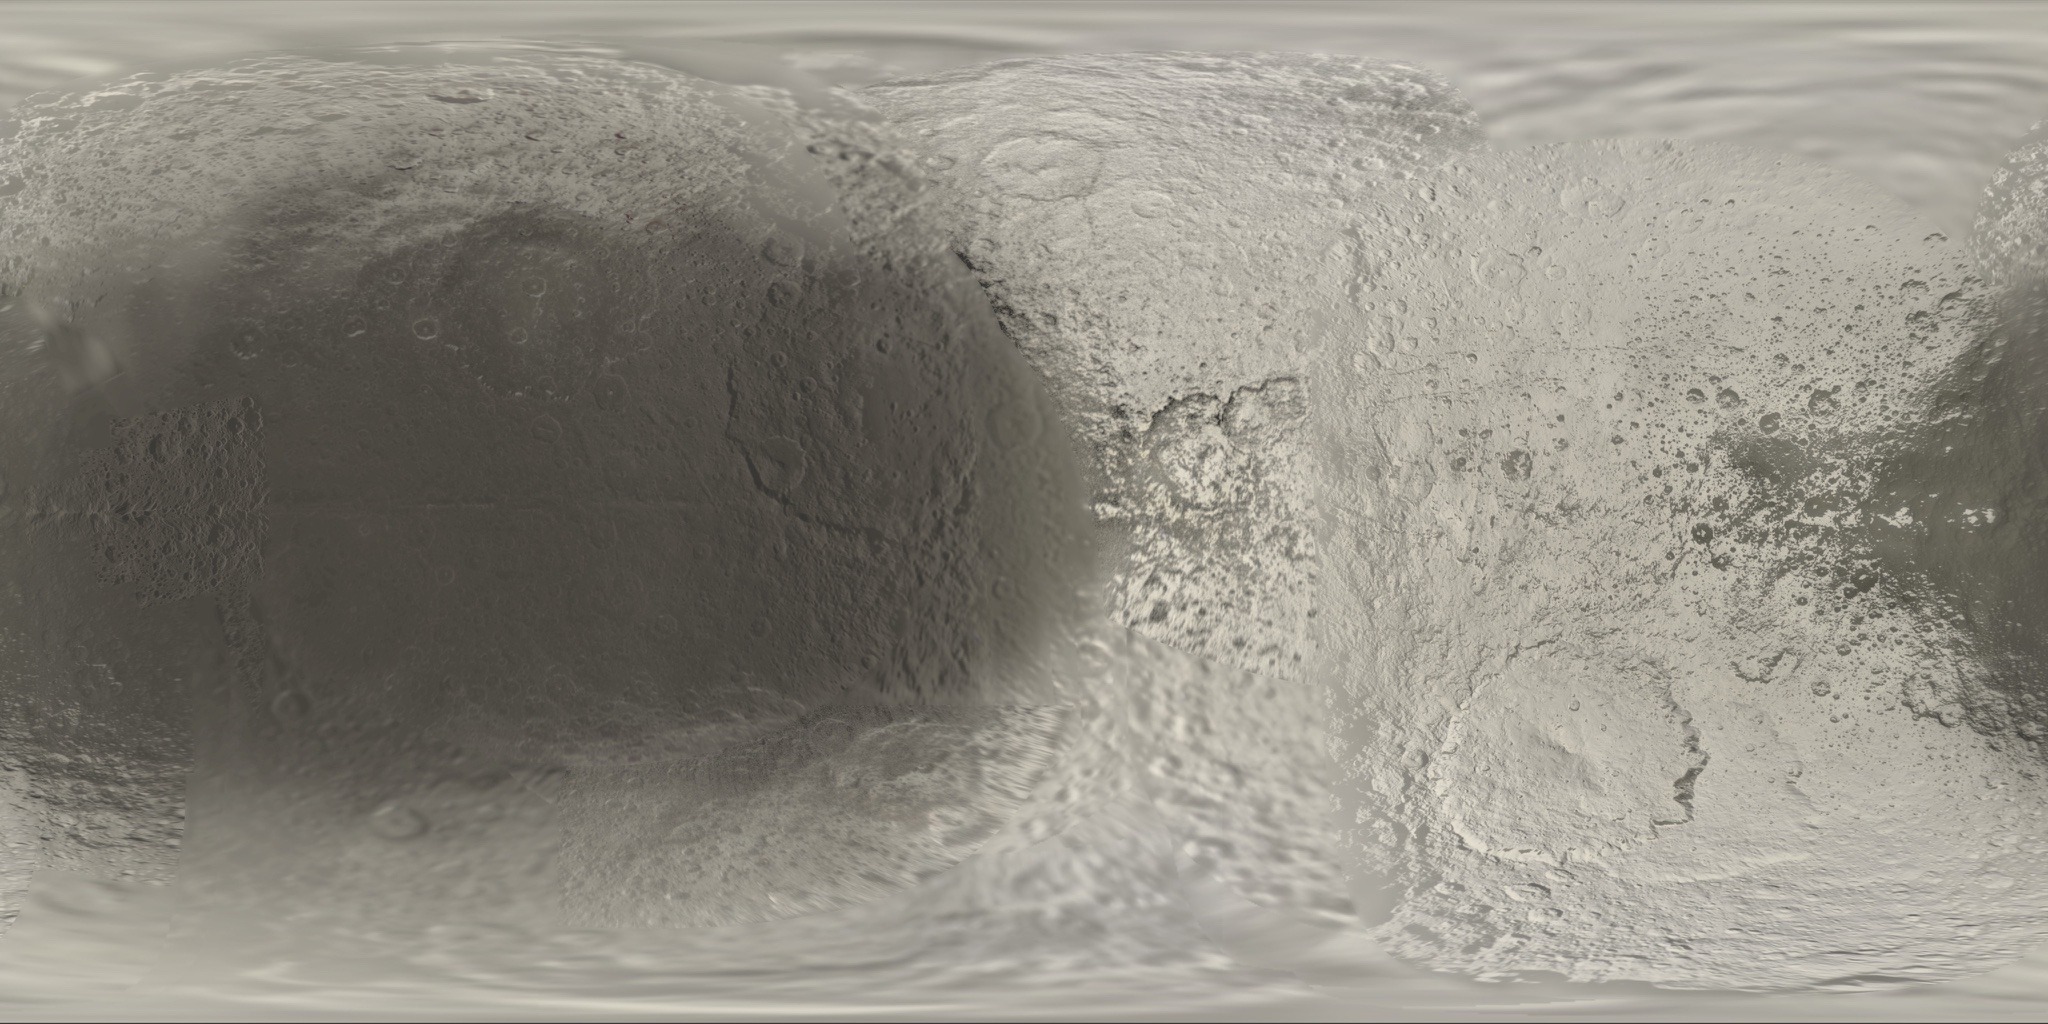
\includegraphics[width=\linewidth,height=4.4cm,keepaspectratio]{../public/textures/hd/iapetus_cassini.jpg}\\[2pt]
{\scriptsize\itshape\color{orbitarMuted} Planiglob desfășurat: Contrastul \quotedblbase{}Yin-Yang\textquotedblright{} dintre emisfera întunecată (Cassini Regio) și emisfera strălucitoare de gheață a lunii Iapetus (NASA/ESA Cassini).}
\end{tabular}
\end{center}


\begin{tcolorbox}[orbitardata, title={\textbf{Repere esențiale: Iapetus}}]
\small
\begin{itemize}[leftmargin=1.4em, itemsep=2pt, topsep=2pt]
  \item \textbf{Clasificare și orbită:} Satelit Natural (Lună) (orbitează în jurul: \textbf{Saturn}) \quad$\bullet$\quad \textbf{Distanță:} 9,582 UA ($\approx$ 1.433 milioane de kilometri)
  \item \textbf{Dimensiuni și masă:} rază medie 734,5 de kilometri \quad$\bullet$\quad masă: 3,00e-4 $\times M_\oplus$
  \item \textbf{Gravitație și regim termic:} 0,023 $\times g_\oplus$ (0,23 m/s$^2$) \quad$\bullet$\quad temperatură medie: -163 $^\circ$C (înclinarea axei: Nespecificată)
  \item \textbf{Ciclu orbital și rotație:} perioadă orbitală (an): 79,32 zile pământești \quad$\bullet$\quad rotație (zi): 1903,70 ore (79,32 zile pământești)
  \item \textbf{Durata călătoriei de pe Pământ:} cu viteza luminii ($1c$): \emph{1 oră și 11 minute}; cu racheta ($50.000$ de kilometri pe oră): \emph{7 ani}; cu avionul ($900$ de kilometri pe oră): \emph{160 de ani}; cu mașina ($100$ de kilometri pe oră): \emph{1.450 de ani}.
  \item \textbf{Repere de scară și curiozitate:} Datorită brâului de munți înalți care o înconjoară exact pe la mijloc, Iapetus seamănă cu o nucă uriașă în două culori! Munții de la ecuatorul lui Iapetus au 20 de kilometri înălțime, depășind de peste două ori înălțimea vârfului Everest de pe Pământ!
\end{itemize}
\end{tcolorbox}

\subsubsection*{Prezentare generală și profil astrofizic}
Descoperită de Giovanni Domenico Cassini în 1671, Iapetus este al treilea satelit ca mărime al lui Saturn. El a observat că satelitul este vizibil prin telescop doar pe o parte a orbitei sale, deducând corect că o emisferă este de 10 ori mai întunecată decât cealaltă. Iapetus este cea mai neobișnuită lună a lui Saturn: o jumătate din ea este neagră ca smoala, iar cealaltă jumătate este albă și strălucitoare ca zăpada! Datorită brâului de munți înalți care o înconjoară exact pe la mijloc, Iapetus seamănă cu o nucă uriașă în două culori!

\subsubsection*{Alcătuirea fizică și structura internă}
Privind în profunzimea sa, alcătuirea fizică este organizată pe mai multe straturi și regiuni distincte, fiecare având un rol bine definit în evoluția și dinamica acestui obiect cosmic. În primul rând se remarcă \textbf{Corp înghețat cu densitate mică (1,088 g/cm$^3$)}, compus în proporție de aproximativ 80\% din gheață de apă și aproximativ 20\% materiale stâncoase. În strânsă legătură cu această componentă se află \textbf{Emisfera întunecată (Cassini Regio) vs. Roncevaux Terra}, unde praful întunecat provenit de la satelitul exterior Phoebe absoarbe căldura solară și sublimează gheața către emisfera rece și albă. În completarea acestui ansamblu întâlnim \textbf{Creasta ecuatorială (1.300 de kilometri lungime)}, un lanț muntos lat de 20 de kilometri și înalt de până la 20 de kilometri care urmează perfect ecuatorul satelitului.

\subsubsection*{Observații astronomice și istoricul explorării}
Fotografiată de Voyager 2 în 1981 și survolată de aproape de sonda Cassini în septembrie 2007. Munții de la ecuatorul lui Iapetus au 20 de kilometri înălțime, depășind de peste două ori înălțimea vârfului Everest de pe Pământ!

\vspace{6pt}
\begin{tcolorbox}[orbitarquiz, title={\textbf{Întrebare de verificare \#22: Iapetus}}]
\textbf{Prin ce se remarcă vizual satelitul Iapetus al lui Saturn?}
\begin{itemize}[leftmargin=2.2em, itemsep=2pt, topsep=4pt]
  \item[$\square$ \textbf{A.}] Are o emisferă neagră ca cărbunele și una albă ca zăpada, plus o creastă muntoasă la ecuator
  \item[$\square$ \textbf{B.}] Este complet verde
  \item[$\square$ \textbf{C.}] Are trei inele proprii de foc
  \item[$\square$ \textbf{D.}] Este cel mai fierbinte corp din Sistemul Solar
\end{itemize}
\vspace{2pt}
{\footnotesize\color{orbitarMuted}\textbf{Răspuns corect:} \textbf{A} (Are o emisferă neagră ca cărbunele și una albă ca zăpada, plus o creastă muntoasă la ecuator). \emph{Iapetus prezintă cel mai dramatic contrast de culoare (albedo) din Sistemul Solar și o creastă ecuatorială care îi dă forma unei nuci.}}
\end{tcolorbox}
\clearpage


\subsection{Phoebe}
\label{sec:body-phoebe}
\vspace{-4pt}
{\large\itshape\color{orbitarAccent} Satelitul întunecat capturat din Centura Kuiper, cu orbită retrogradă în jurul lui Saturn}\\[4pt]


\begin{center}
\begin{tabular}{@{}m{0.44\textwidth}@{\hspace{0.03\textwidth}}m{0.51\textwidth}@{}}
\centering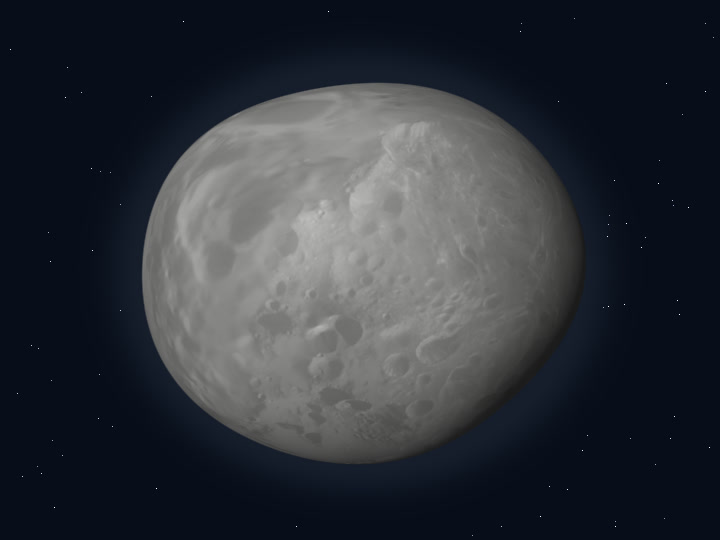
\includegraphics[width=\linewidth,height=4.4cm,keepaspectratio]{imagini/globuri/phoebe.jpg}\\[2pt]
{\scriptsize\itshape\color{orbitarMuted} Vedere 3D a corpului ceresc (\textbf{Phoebe})}
&
\centering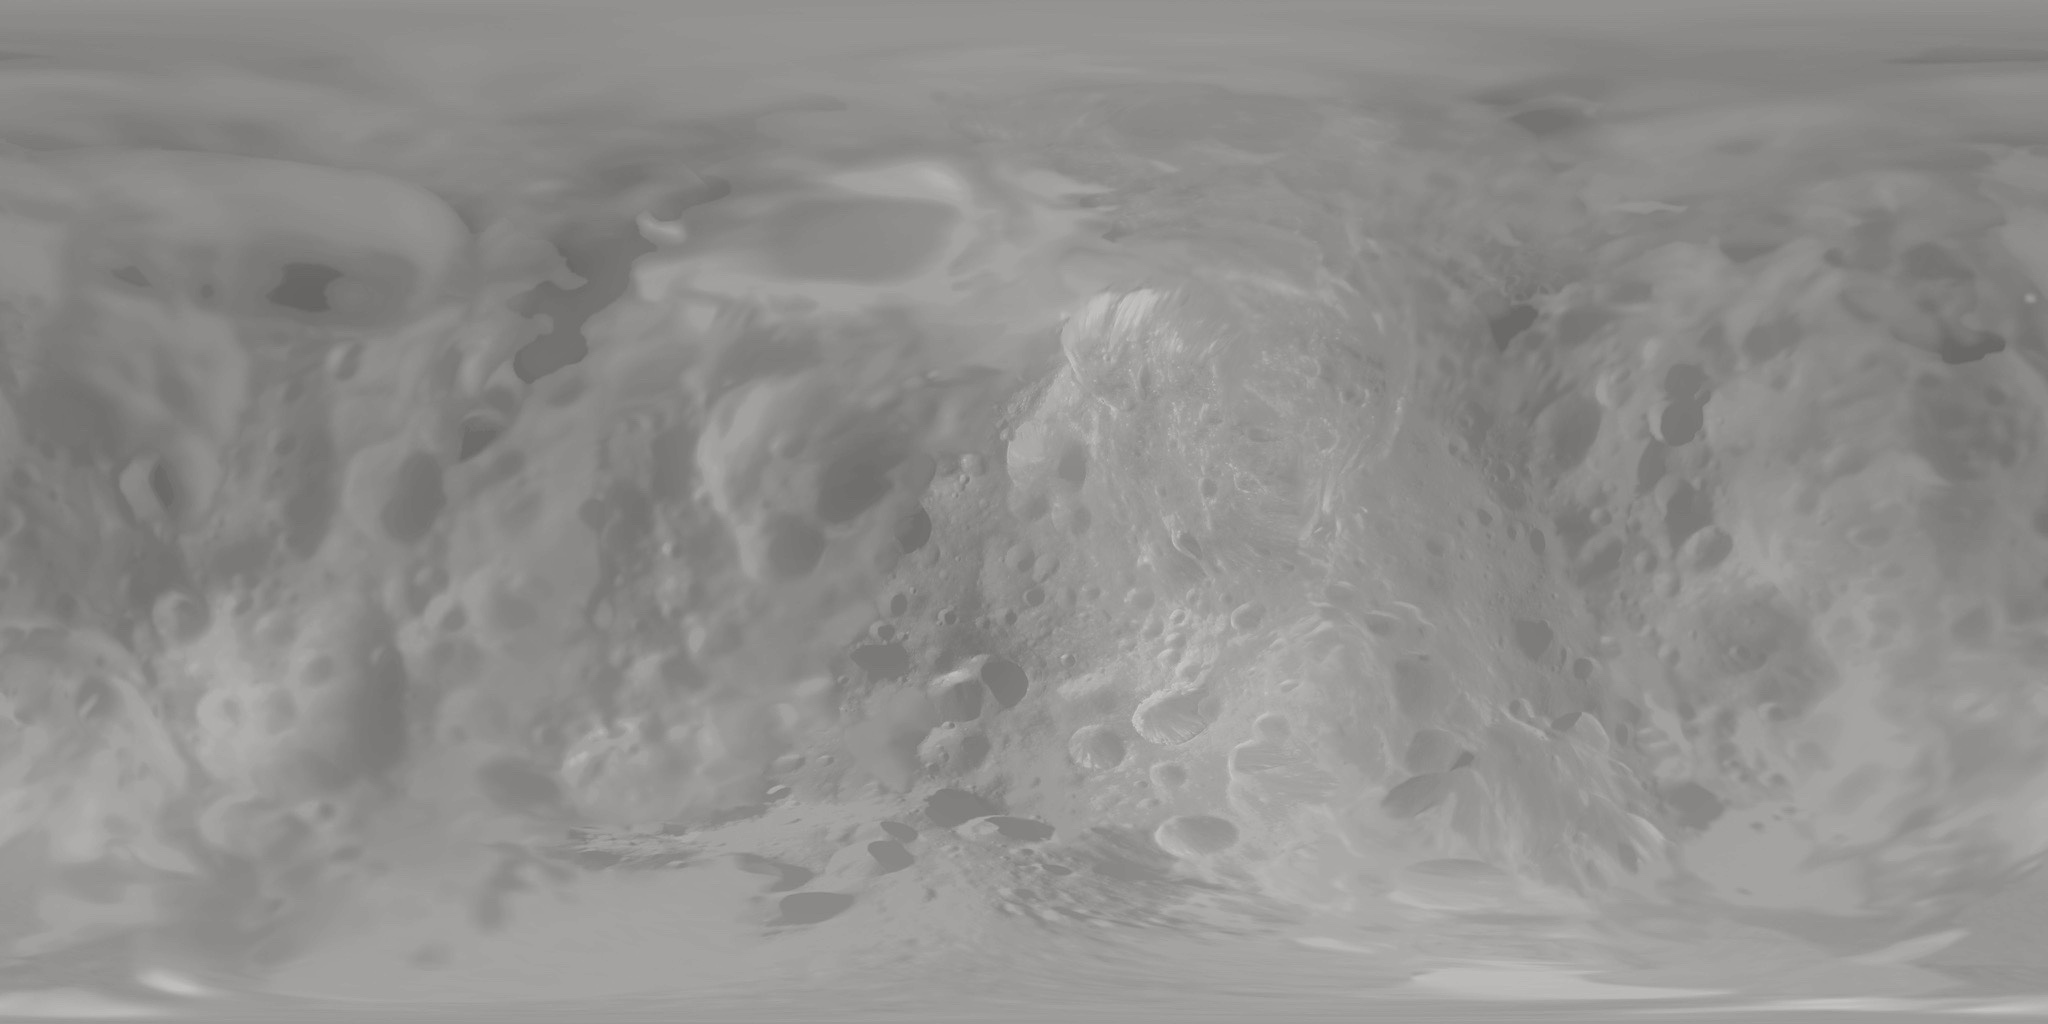
\includegraphics[width=\linewidth,height=4.4cm,keepaspectratio]{../public/textures/hd/phoebe_cassini.jpg}\\[2pt]
{\scriptsize\itshape\color{orbitarMuted} Planiglob desfășurat: Harta satelitului retrograd Phoebe (planetozimal capturat din Centura Kuiper) și a craterului Jason (NASA/ESA Cassini).}
\end{tabular}
\end{center}


\begin{tcolorbox}[orbitardata, title={\textbf{Repere esențiale: Phoebe}}]
\small
\begin{itemize}[leftmargin=1.4em, itemsep=2pt, topsep=2pt]
  \item \textbf{Clasificare și orbită:} Satelit Natural (Lună) (orbitează în jurul: \textbf{Saturn}) \quad$\bullet$\quad \textbf{Distanță:} 9,582 UA ($\approx$ 1.433 milioane de kilometri)
  \item \textbf{Dimensiuni și masă:} rază medie 106,5 kilometri \quad$\bullet$\quad masă: 1,39e-6 $\times M_\oplus$
  \item \textbf{Gravitație și regim termic:} 0,004 $\times g_\oplus$ (0,04 m/s$^2$) \quad$\bullet$\quad temperatură medie: -198 $^\circ$C (înclinarea axei: Nespecificată)
  \item \textbf{Ciclu orbital și rotație:} perioadă orbitală (an): 550,31 zile pământești (Orbită retrogradă!) \quad$\bullet$\quad rotație (zi): 9,27 ore (0,39 zile pământești)
  \item \textbf{Durata călătoriei de pe Pământ:} cu viteza luminii ($1c$): \emph{1 oră și 11 minute}; cu racheta ($50.000$ de kilometri pe oră): \emph{7 ani}; cu avionul ($900$ de kilometri pe oră): \emph{160 de ani}; cu mașina ($100$ de kilometri pe oră): \emph{1.450 de ani}.
  \item \textbf{Repere de scară și curiozitate:} La fel ca Triton la Neptun, Phoebe zboară \guillemotleft{}pe contrasens\guillemotright{} în jurul lui Saturn, la o distanță uriașă de aproape 13 milioane de kilometri! Phoebe a fost primul satelit descoperit vreodată cu ajutorul fotografiilor astronomice, în anul 1899, și lasă în urma lui cel mai mare inel de praf al lui Saturn!
\end{itemize}
\end{tcolorbox}

\subsubsection*{Prezentare generală și profil astrofizic}
Descoperită în 1899 de William Henry Pickering pe plăci fotografice, Phoebe (diametru mediu 213 kilometri) orbitează retrograd la 12,9 milioane de kilometri de Saturn în 550 de zile. Densitatea ridicată (1,63 g/cm$^3$) și compoziția isotopică arată că este un centaur primordial capturat din Centura Kuiper. Phoebe este un călător misterios de la marginea Sistemului Solar care a fost prins de gravitația lui Saturn! Este negru ca cărbunele la exterior, dar ascunde gheață albă sub praf. La fel ca Triton la Neptun, Phoebe zboară \guillemotleft{}pe contrasens\guillemotright{} în jurul lui Saturn, la o distanță uriașă de aproape 13 milioane de kilometri!

\subsubsection*{Alcătuirea fizică și structura internă}
Privind în profunzimea sa, alcătuirea fizică este organizată pe mai multe straturi și regiuni distincte, fiecare având un rol bine definit în evoluția și dinamica acestui obiect cosmic. În primul rând se remarcă \textbf{Interior dens de rocă și gheață (1,63 g/cm$^3$)}, compoziție similară cu cea a lui Pluto și Triton, mult mai bogată în rocă decât lunile interioare ale lui Saturn. În strânsă legătură cu această componentă se află \textbf{Craterul gigant Jason (101 kilometri diametru)}, impacturile meteoritice au îndepărtat pătura neagră de compuși organici și filosilicați, dezvăluind pereți strălucitori de gheață de apă. În completarea acestui ansamblu întâlnim \textbf{Sursa gigantului \guillemotleft{}Inel Phoebe\guillemotright{}}, micrometeoriții lovesc continuu Phoebe și ridică un inel vast de praf întunecat care cade în spirală și înnegrește emisfera anterioară a lui Iapetus.

\subsubsection*{Observații astronomice și istoricul explorării}
A fost prima țintă studiată de sonda Cassini la sosirea în sistemul lui Saturn, printr-un survol la 2.068 de kilometri distanță pe 11 iunie 2004. Phoebe a fost primul satelit descoperit vreodată cu ajutorul fotografiilor astronomice, în anul 1899, și lasă în urma lui cel mai mare inel de praf al lui Saturn!

\vspace{6pt}
\begin{tcolorbox}[orbitarquiz, title={\textbf{Întrebare de verificare \#23: Phoebe}}]
\textbf{Care este originea satelitului exterior Phoebe al lui Saturn și ce efect produce praful desprins de pe el?}
\begin{itemize}[leftmargin=2.2em, itemsep=2pt, topsep=4pt]
  \item[$\square$ \textbf{A.}] Este un corp capturat din Centura Kuiper, iar praful său întunecat colorează în negru o emisferă a satelitului Iapetus
  \item[$\square$ \textbf{B.}] Este o bucată din Soare
  \item[$\square$ \textbf{C.}] Este făcut din gaz hidrogen
  \item[$\square$ \textbf{D.}] Orbitează în interiorul inelelor principale
\end{itemize}
\vspace{2pt}
{\footnotesize\color{orbitarMuted}\textbf{Răspuns corect:} \textbf{A} (Este un corp capturat din Centura Kuiper, iar praful său întunecat colorează în negru o emisferă a satelitului Iapetus). \emph{Orbita retrogradă și compoziția lui Phoebe confirmă că a fost capturat din Centura Kuiper, iar praful din Inelul Phoebe este responsabil pentru emisfera întunecată a lui Iapetus.}}
\end{tcolorbox}
\clearpage


\section{Uranus}
\label{sec:body-uranus}
\vspace{-4pt}
{\large\itshape\color{orbitarAccent} Gigantul de gheață turcoaz care se rostogolește pe orbită}\\[4pt]


\begin{center}
\begin{tabular}{@{}m{0.44\textwidth}@{\hspace{0.03\textwidth}}m{0.51\textwidth}@{}}
\centering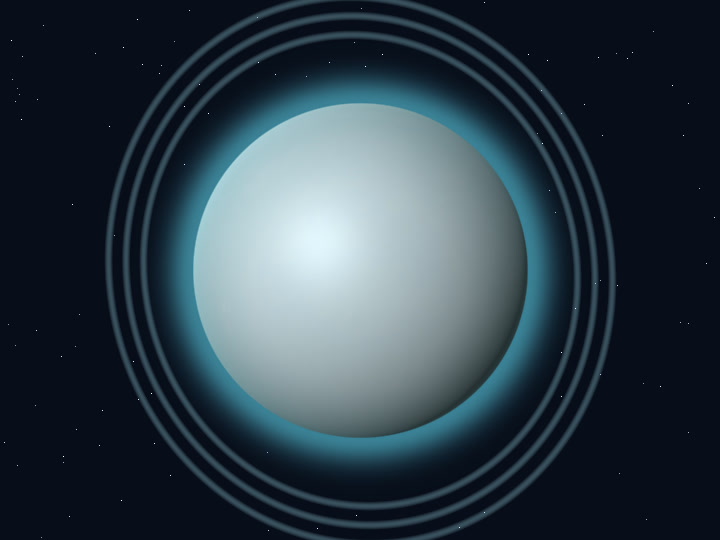
\includegraphics[width=\linewidth,height=4.4cm,keepaspectratio]{imagini/globuri/uranus.jpg}\\[2pt]
{\scriptsize\itshape\color{orbitarMuted} Vedere 3D a corpului ceresc (\textbf{Uranus})}
&
\centering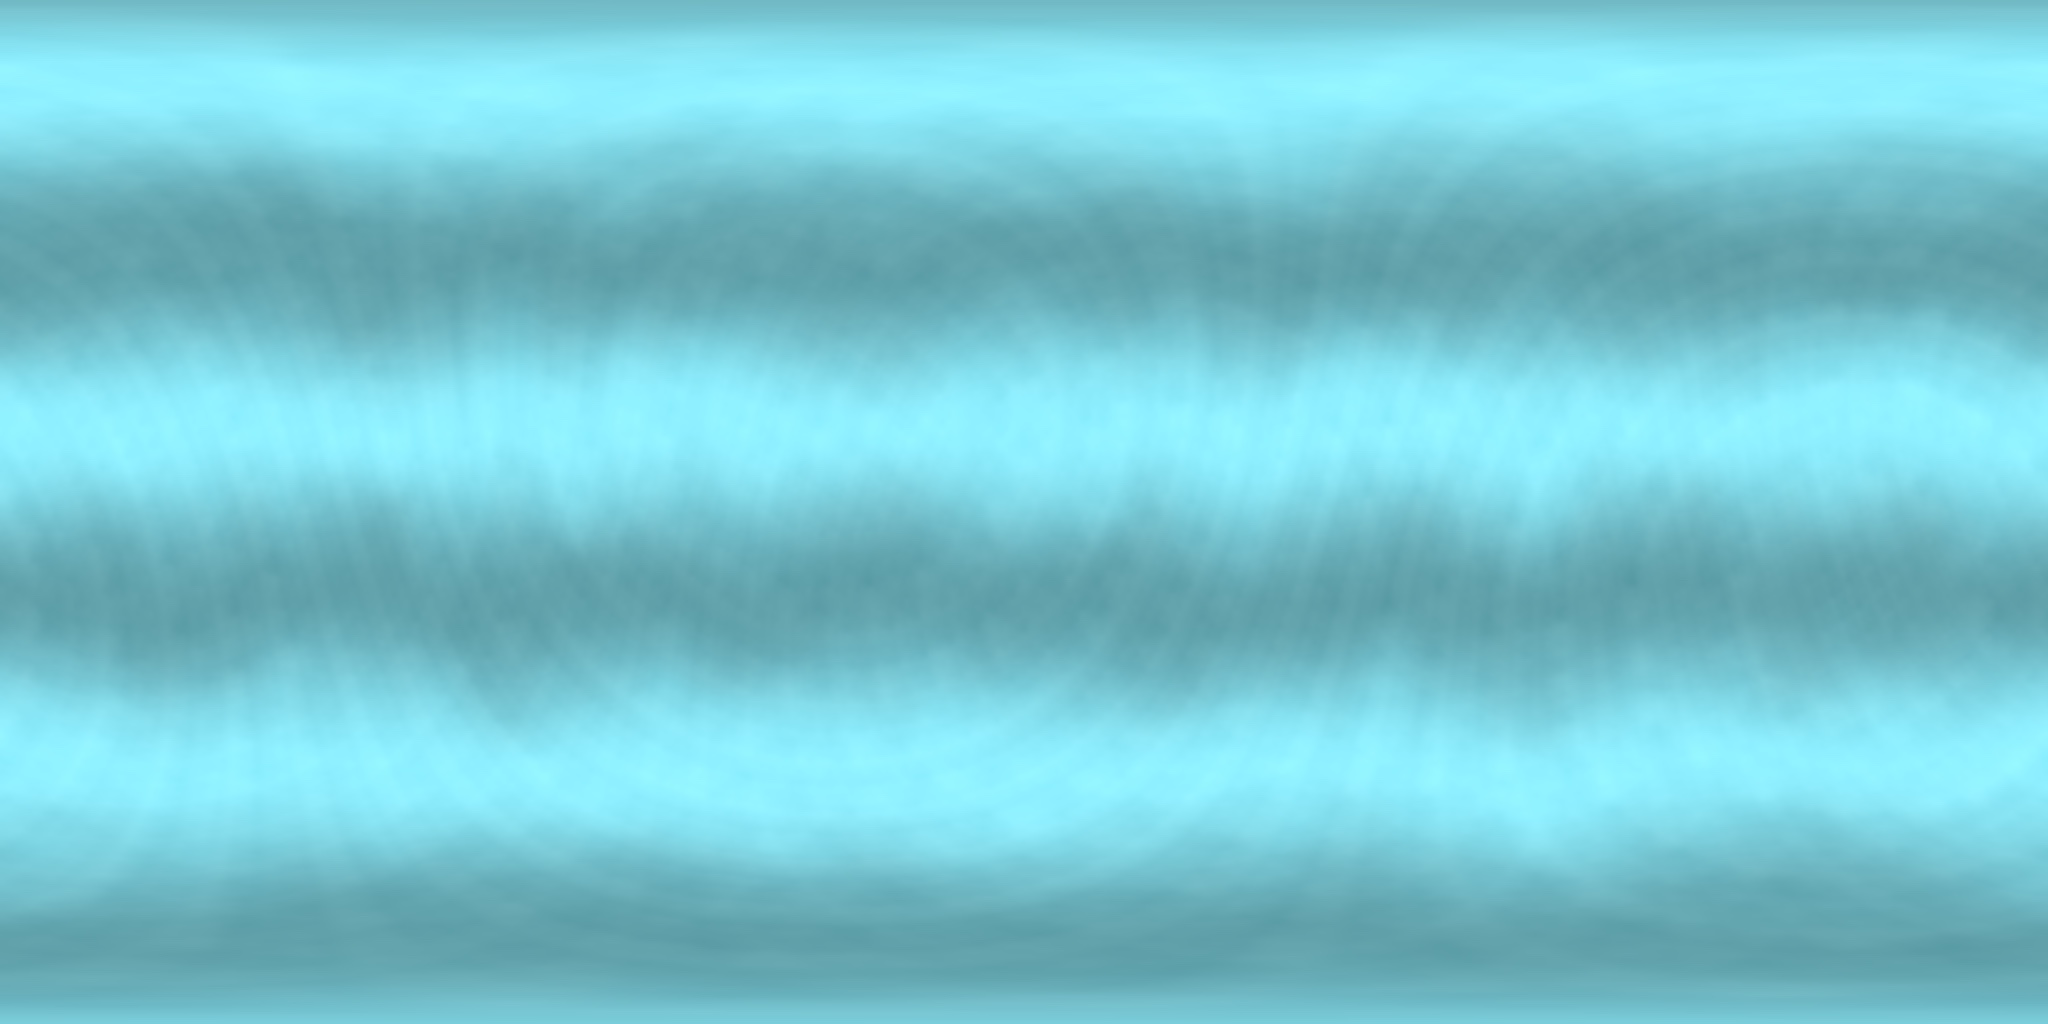
\includegraphics[width=\linewidth,height=4.4cm,keepaspectratio]{../public/textures/hd/uranus_voyager.jpg}\\[2pt]
{\scriptsize\itshape\color{orbitarMuted} Planiglob desfășurat: Harta atmosferei de hidrogen, heliu și metan a gigantului de gheață Uranus (date NASA Voyager 2).}
\end{tabular}
\end{center}


\begin{tcolorbox}[orbitardata, title={\textbf{Repere esențiale: Uranus}}]
\small
\begin{itemize}[leftmargin=1.4em, itemsep=2pt, topsep=2pt]
  \item \textbf{Clasificare și orbită:} Gigant de Gheață \quad$\bullet$\quad \textbf{Distanță:} 19,218 UA ($\approx$ 2.875 milioane de kilometri)
  \item \textbf{Dimensiuni și masă:} rază medie 25.362 de kilometri \quad$\bullet$\quad masă: 14,540 $\times M_\oplus$
  \item \textbf{Gravitație și regim termic:} 0,890 $\times g_\oplus$ (8,73 m/s$^2$) \quad$\bullet$\quad temperatură medie: -195 $^\circ$C (înclinarea axei: 97,77$^\circ$)
  \item \textbf{Ciclu orbital și rotație:} perioadă orbitală (an): 30.688,5 zile ($\approx$ 84,02 ani pământești) \quad$\bullet$\quad rotație (zi): 17,24 ore (Rotație retrogradă!)
  \item \textbf{Durata călătoriei de pe Pământ:} cu viteza luminii ($1c$): \emph{2 ore și 30 de minute}; cu racheta ($50.000$ de kilometri pe oră): \emph{8 ani și jumătate}; cu avionul ($900$ de kilometri pe oră): \emph{345 de ani}; cu mașina ($100$ de kilometri pe oră): \emph{3.100 de ani}.
  \item \textbf{Repere de scară și curiozitate:} Dacă Pământul e o mărgea, Uranus e cât un măr mare de culoarea gheții! Un anotimp pe Uranus durează 21 de ani pământești de lumină continuă sau de întuneric!
\end{itemize}
\end{tcolorbox}

\subsubsection*{Prezentare generală și profil astrofizic}
Prima planetă descoperită cu ajutorul telescopului (William Herschel, 1781), Uranus este clasificată drept \guillemotleft{}gigant de gheață\guillemotright{}. Înclinarea axială extremă de 97,77$^\circ$ este atribuită unei coliziuni cataclismice cu o protoplanetă în tinerețea Sistemului Solar. Uranus este o planetă de culoare bleu-turcoaz care face ceva unic: în loc să se învârtă ca un titirez drept, stă culcată pe o parte și se rostogolește ca o minge! Dacă Pământul e o mărgea, Uranus e cât un măr mare de culoarea gheții!

\subsubsection*{Alcătuirea fizică și structura internă}
Privind în profunzimea sa, alcătuirea fizică este organizată pe mai multe straturi și regiuni distincte, fiecare având un rol bine definit în evoluția și dinamica acestui obiect cosmic. În primul rând se remarcă \textbf{Nucleu silicat-metalic rece}, de dimensiuni relativ reduse, emițând foarte puțină căldură internă. În strânsă legătură cu această componentă se află \textbf{Manta fluidă de \guillemotleft{}ghețuri\guillemotright{}}, amestec dens și fierbinte de apă, amoniac și metan aflate la presiuni extreme. În completarea acestui ansamblu întâlnim \textbf{Atmosferă de hidrogen, heliu și metan}, unde metanul absoarbe lumina roșie a Soarelui și reflectă nuanța caracteristică cyan.

\subsubsection*{Observații astronomice și istoricul explorării}
Descoperită în 1781 și vizitată de o singură navă spațială până în prezent: Voyager 2 în ianuarie 1986. Un anotimp pe Uranus durează 21 de ani pământești de lumină continuă sau de întuneric!

\vspace{6pt}
\begin{tcolorbox}[orbitarquiz, title={\textbf{Întrebare de verificare \#24: Uranus}}]
\textbf{Ce gaz din atmosfera lui Uranus îi oferă culoarea turcoaz (cyan)?}
\begin{itemize}[leftmargin=2.2em, itemsep=2pt, topsep=4pt]
  \item[$\square$ \textbf{A.}] Oxigenul
  \item[$\square$ \textbf{B.}] Dioxidul de carbon
  \item[$\square$ \textbf{C.}] Metanul
  \item[$\square$ \textbf{D.}] Azotul
\end{itemize}
\vspace{2pt}
{\footnotesize\color{orbitarMuted}\textbf{Răspuns corect:} \textbf{C} (Metanul). \emph{Metanul (CH$_4$) din atmosfera superioară absoarbe componenta roșie a luminii solare și difuzează lumina albastră-verzuie.}}
\end{tcolorbox}
\clearpage


\subsection{Miranda}
\label{sec:body-miranda}
\vspace{-4pt}
{\large\itshape\color{orbitarAccent} Luna-puzzle a lui Uranus, cu cea mai înaltă stâncă din Sistemul Solar}\\[4pt]


\begin{center}
\begin{tabular}{@{}m{0.44\textwidth}@{\hspace{0.03\textwidth}}m{0.51\textwidth}@{}}
\centering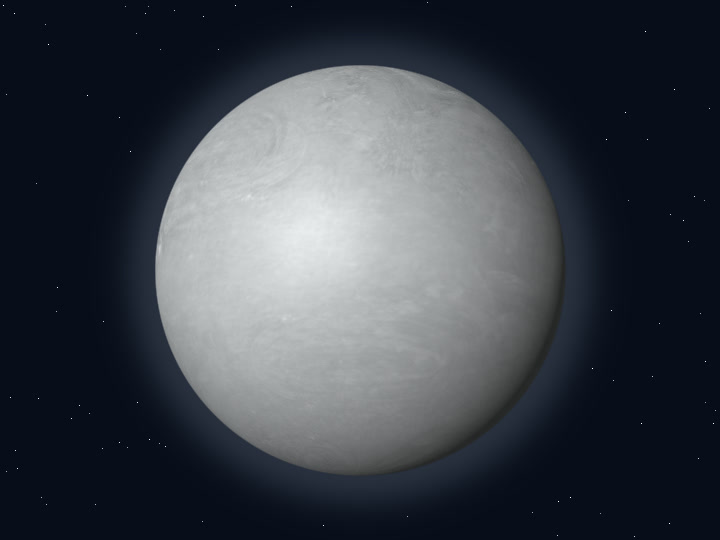
\includegraphics[width=\linewidth,height=4.4cm,keepaspectratio]{imagini/globuri/miranda.jpg}\\[2pt]
{\scriptsize\itshape\color{orbitarMuted} Vedere 3D a corpului ceresc (\textbf{Miranda})}
&
\centering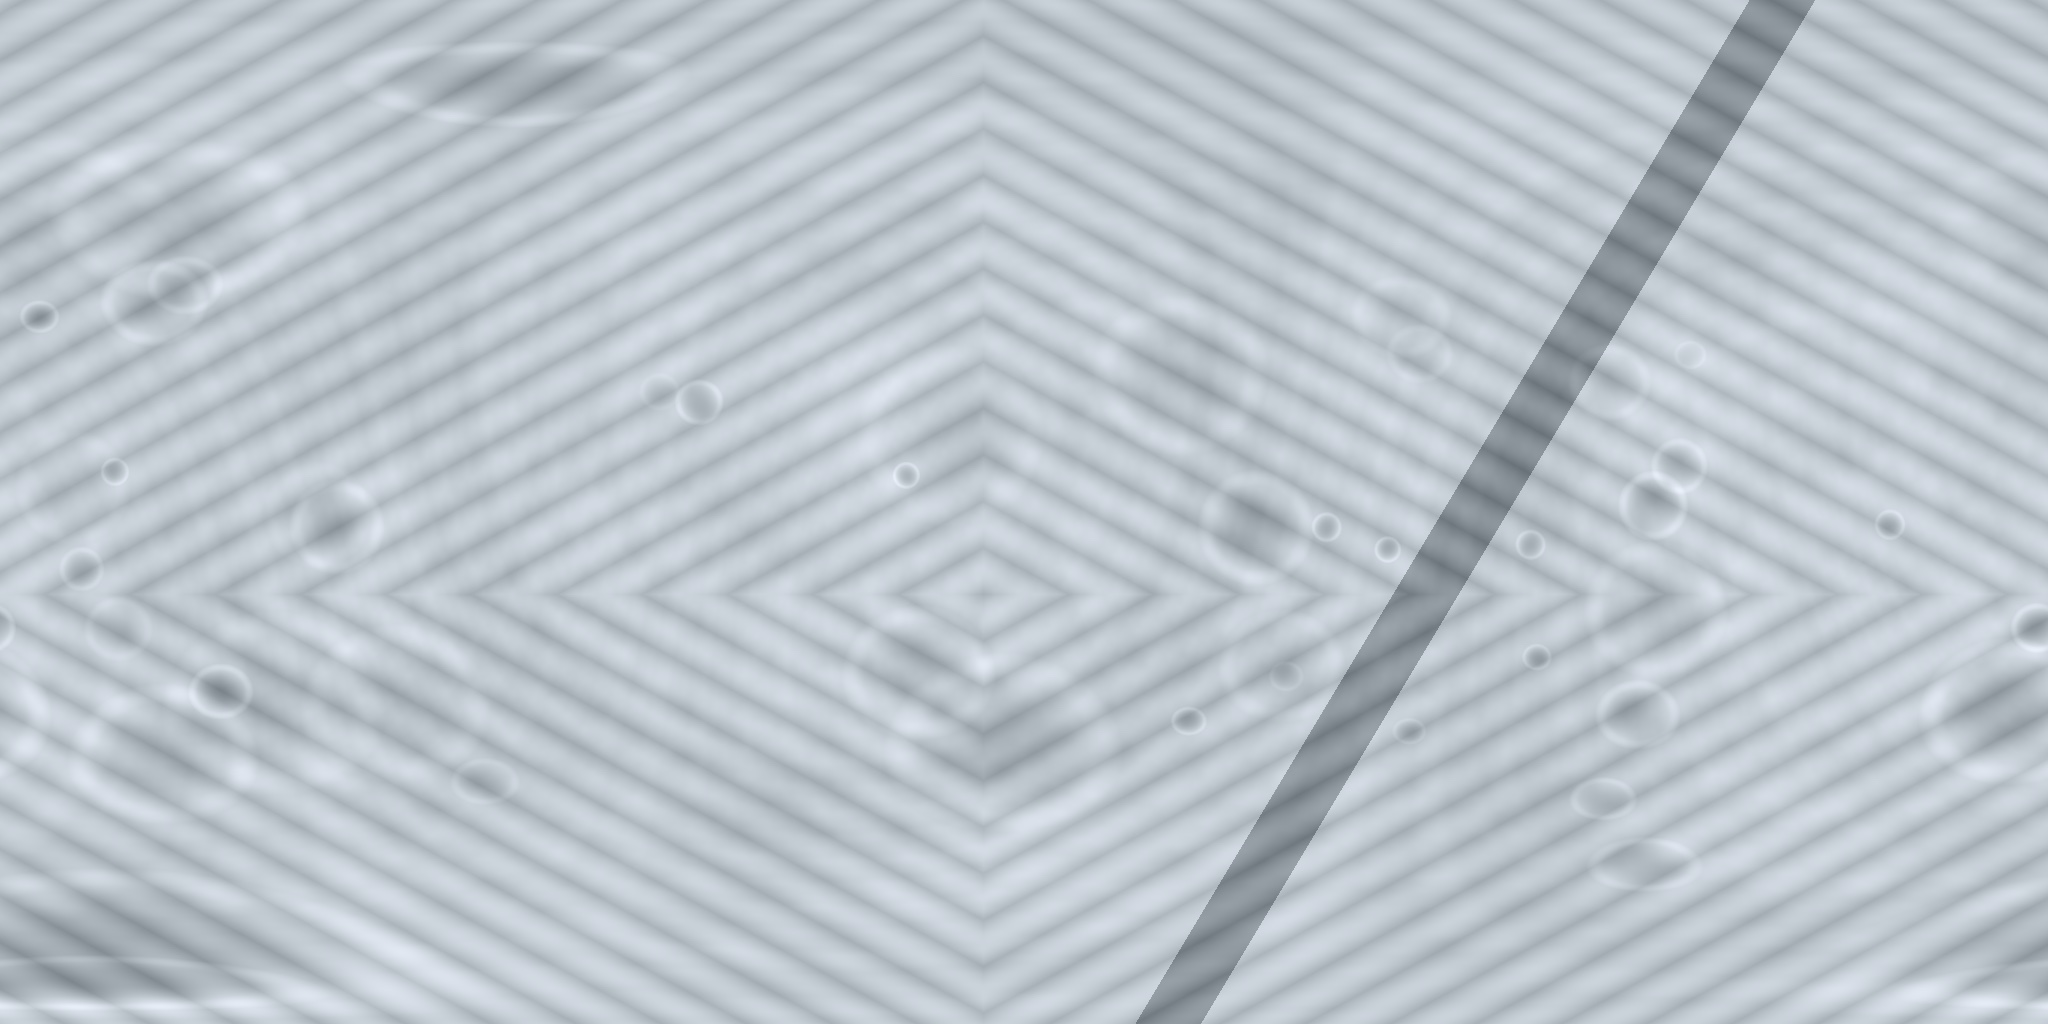
\includegraphics[width=\linewidth,height=4.4cm,keepaspectratio]{../public/textures/hd/miranda_voyager.jpg}\\[2pt]
{\scriptsize\itshape\color{orbitarMuted} Planiglob desfășurat: Relieful spectaculos al lunii Miranda, cu stâncile Verona Rupes și regiunile coronae (NASA Voyager 2).}
\end{tabular}
\end{center}


\begin{tcolorbox}[orbitardata, title={\textbf{Repere esențiale: Miranda}}]
\small
\begin{itemize}[leftmargin=1.4em, itemsep=2pt, topsep=2pt]
  \item \textbf{Clasificare și orbită:} Satelit Natural (Lună) (orbitează în jurul: \textbf{Uranus}) \quad$\bullet$\quad \textbf{Distanță:} 19,218 UA ($\approx$ 2.875 milioane de kilometri)
  \item \textbf{Dimensiuni și masă:} rază medie 235,8 de kilometri \quad$\bullet$\quad masă: 1,10e-5 $\times M_\oplus$
  \item \textbf{Gravitație și regim termic:} 0,008 $\times g_\oplus$ (0,08 m/s$^2$) \quad$\bullet$\quad temperatură medie: -213 $^\circ$C (înclinarea axei: Nespecificată)
  \item \textbf{Ciclu orbital și rotație:} perioadă orbitală (an): 1,413 zile pământești \quad$\bullet$\quad rotație (zi): 33,90 ore (1,41 zile pământești)
  \item \textbf{Durata călătoriei de pe Pământ:} cu viteza luminii ($1c$): \emph{2 ore și 30 de minute}; cu racheta ($50.000$ de kilometri pe oră): \emph{8 ani și jumătate}; cu avionul ($900$ de kilometri pe oră): \emph{345 de ani}; cu mașina ($100$ de kilometri pe oră): \emph{3.100 de ani}.
  \item \textbf{Repere de scară și curiozitate:} Pe Miranda se află Verona Rupes, o prăpastie de gheață atât de înaltă încât, dacă ai sări de pe marginea ei, ai pluti în cădere timp de 12 minute până jos! Stânca Verona Rupes are 20 de kilometri înălțime și este cea mai înaltă prăpastie din întregul Sistem Solar!
\end{itemize}
\end{tcolorbox}

\subsubsection*{Prezentare generală și profil astrofizic}
Descoperită de Gerard Kuiper în 1948, Miranda este cea mai interioară și mai mică dintre cele cinci luni majore ale lui Uranus. Suprafața ei prezintă cel mai extrem relief tectonic raportat la dimensiunea sa, cu canioane de 12 ori mai adânci decât Marele Canion. Miranda este o lună mică și uimitoare a lui Uranus, care arată de parcă a fost lipită la loc din piese diferite de puzzle de gheață! Pe Miranda se află Verona Rupes, o prăpastie de gheață atât de înaltă încât, dacă ai sări de pe marginea ei, ai pluti în cădere timp de 12 minute până jos!

\subsubsection*{Alcătuirea fizică și structura internă}
Privind în profunzimea sa, alcătuirea fizică este organizată pe mai multe straturi și regiuni distincte, fiecare având un rol bine definit în evoluția și dinamica acestui obiect cosmic. În primul rând se remarcă \textbf{Nucleu de silicați și manta de gheață}, încălzită în trecut de rezonanțe orbitale cu ceilalți sateliți ai lui Uranus. În strânsă legătură cu această componentă se află \textbf{Coronae (Inverness, Arden, Elsinore)}, trei regiuni poligonale uriașe (peste 200 de kilometri lățime) cu creste și șanțuri concentrice în formă de chevron. În completarea acestui ansamblu întâlnim \textbf{Verona Rupes}, falie tectonică verticală de gheață cu o înălțime estimată la 20 de kilometri.

\subsubsection*{Observații astronomice și istoricul explorării}
Survolată de aproape de sonda Voyager 2 la 24 ianuarie 1986, care a transmis singurele imagini detaliate ale suprafeței sale. Stânca Verona Rupes are 20 de kilometri înălțime și este cea mai înaltă prăpastie din întregul Sistem Solar!

\vspace{6pt}
\begin{tcolorbox}[orbitarquiz, title={\textbf{Întrebare de verificare \#25: Miranda}}]
\textbf{Ce record deține stânca Verona Rupes de pe satelitul Miranda al lui Uranus?}
\begin{itemize}[leftmargin=2.2em, itemsep=2pt, topsep=4pt]
  \item[$\square$ \textbf{A.}] Este cel mai fierbinte vulcan
  \item[$\square$ \textbf{B.}] Este cea mai înaltă faleză (prăpastie) cunoscută din Sistemul Solar (aproximativ 20 de kilometri înălțime)
  \item[$\square$ \textbf{C.}] Este cel mai adânc ocean
  \item[$\square$ \textbf{D.}] Este cel mai lung râu de metan
\end{itemize}
\vspace{2pt}
{\footnotesize\color{orbitarMuted}\textbf{Răspuns corect:} \textbf{B} (Este cea mai înaltă faleză (prăpastie) cunoscută din Sistemul Solar (aproximativ 20 de kilometri înălțime)). \emph{Verona Rupes se ridică la aproximativ 20 de kilometri deasupra terenului înconjurător, fiind de peste două ori mai înaltă decât muntele Everest.}}
\end{tcolorbox}
\clearpage


\subsection{Ariel}
\label{sec:body-ariel}
\vspace{-4pt}
{\large\itshape\color{orbitarAccent} Cea mai luminoasă lună a lui Uranus, străbătută de văi tectonice și câmpii netede}\\[4pt]


\begin{center}
\begin{tabular}{@{}m{0.44\textwidth}@{\hspace{0.03\textwidth}}m{0.51\textwidth}@{}}
\centering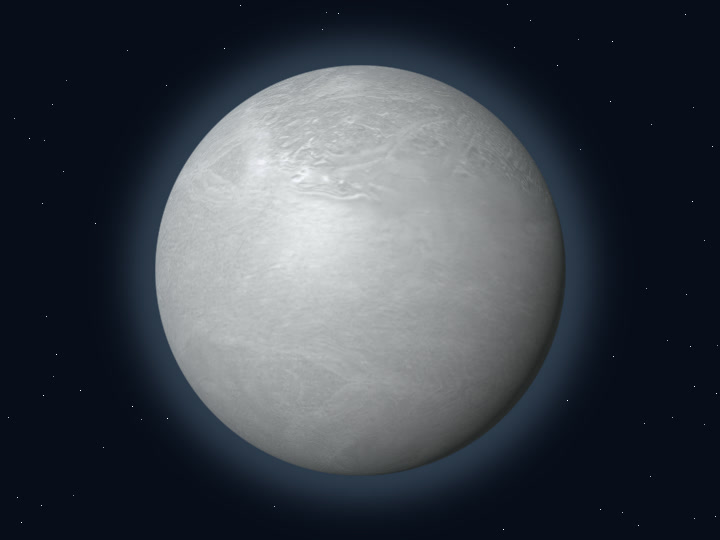
\includegraphics[width=\linewidth,height=4.4cm,keepaspectratio]{imagini/globuri/ariel.jpg}\\[2pt]
{\scriptsize\itshape\color{orbitarMuted} Vedere 3D a corpului ceresc (\textbf{Ariel})}
&
\centering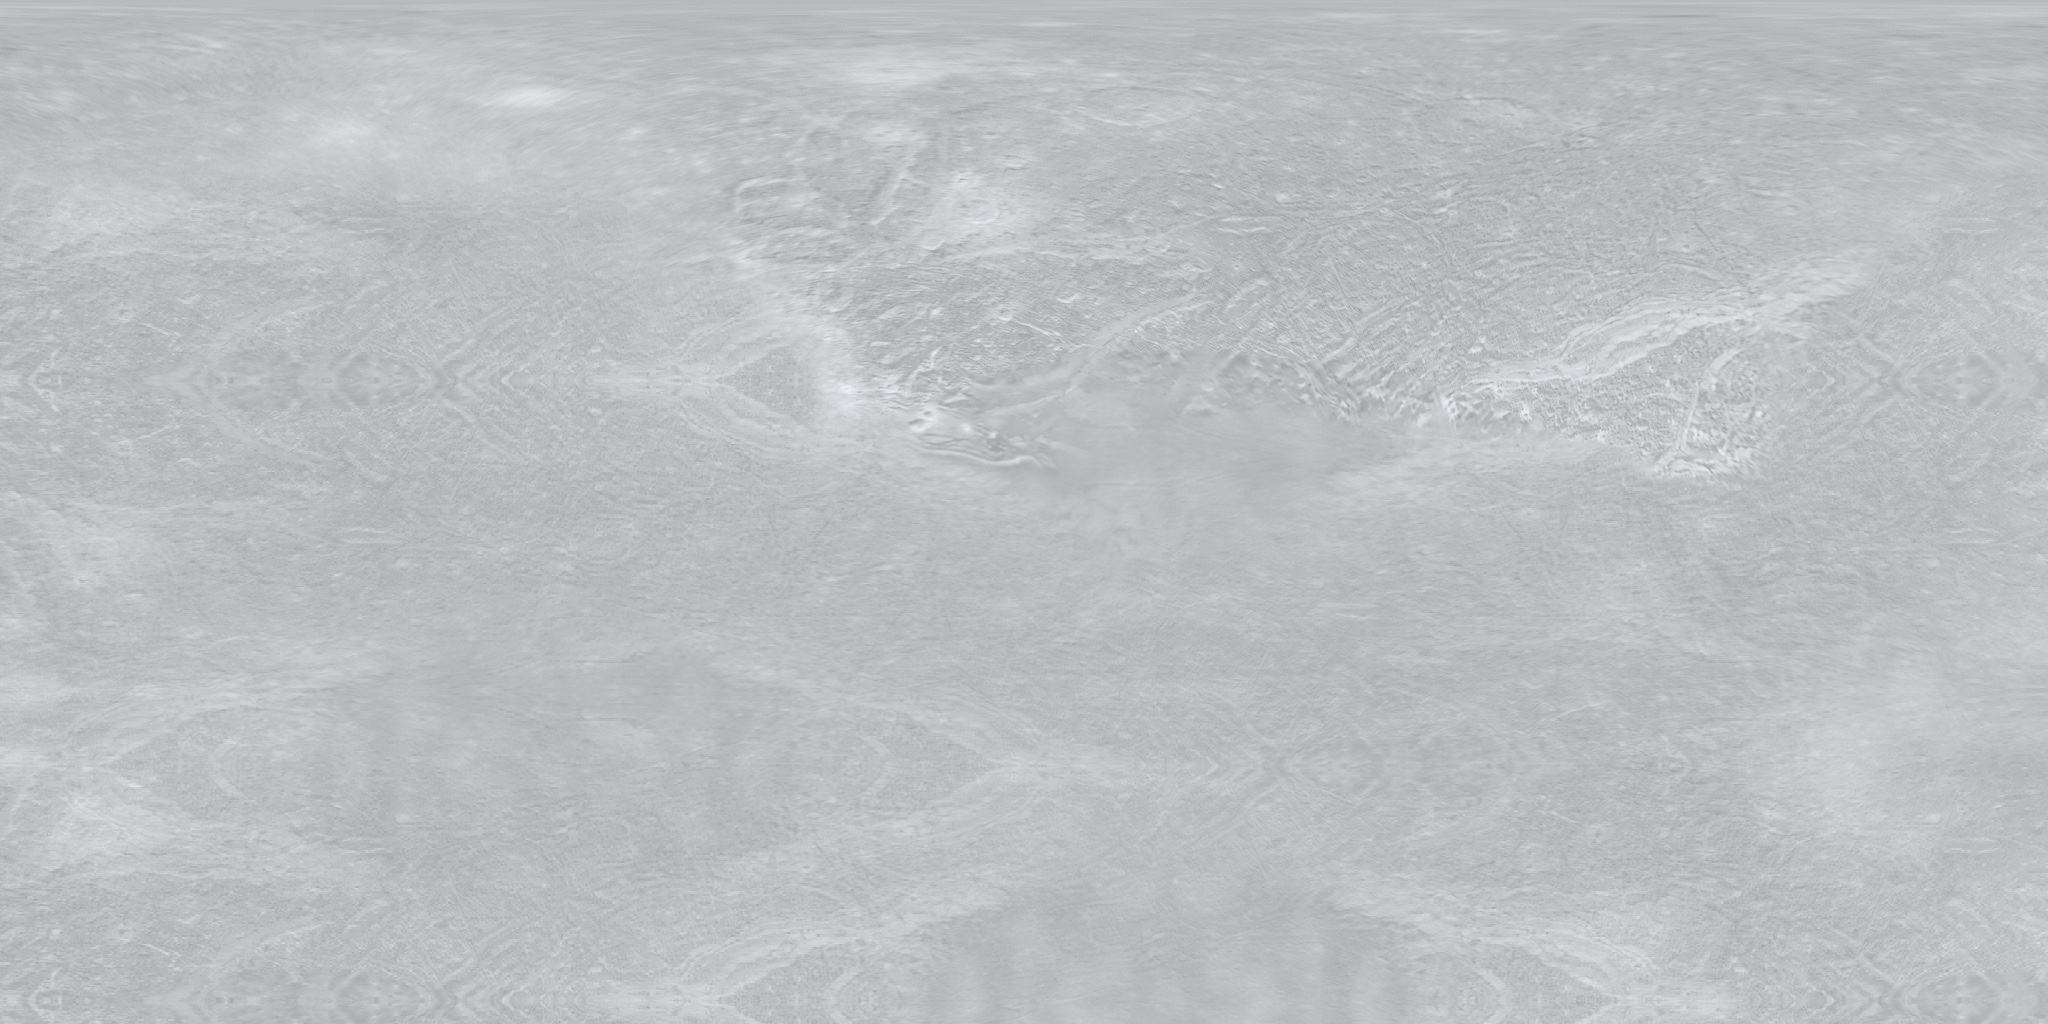
\includegraphics[width=\linewidth,height=4.4cm,keepaspectratio]{../public/textures/hd/ariel_voyager.jpg}\\[2pt]
{\scriptsize\itshape\color{orbitarMuted} Planiglob desfășurat: Harta celei mai luminoase luni a lui Uranus, Ariel, brăzdată de canioanele tectonice Kachina Chasmata (NASA Voyager 2).}
\end{tabular}
\end{center}


\begin{tcolorbox}[orbitardata, title={\textbf{Repere esențiale: Ariel}}]
\small
\begin{itemize}[leftmargin=1.4em, itemsep=2pt, topsep=2pt]
  \item \textbf{Clasificare și orbită:} Satelit Natural (Lună) (orbitează în jurul: \textbf{Uranus}) \quad$\bullet$\quad \textbf{Distanță:} 19,218 UA ($\approx$ 2.875 milioane de kilometri)
  \item \textbf{Dimensiuni și masă:} rază medie 578,9 de kilometri \quad$\bullet$\quad masă: 2,09e-4 $\times M_\oplus$
  \item \textbf{Gravitație și regim termic:} 0,025 $\times g_\oplus$ (0,25 m/s$^2$) \quad$\bullet$\quad temperatură medie: -213 $^\circ$C (înclinarea axei: Nespecificată)
  \item \textbf{Ciclu orbital și rotație:} perioadă orbitală (an): 2,52 zile pământești \quad$\bullet$\quad rotație (zi): 60,49 ore (2,52 zile pământești)
  \item \textbf{Durata călătoriei de pe Pământ:} cu viteza luminii ($1c$): \emph{2 ore și 30 de minute}; cu racheta ($50.000$ de kilometri pe oră): \emph{8 ani și jumătate}; cu avionul ($900$ de kilometri pe oră): \emph{345 de ani}; cu mașina ($100$ de kilometri pe oră): \emph{3.100 de ani}.
  \item \textbf{Repere de scară și curiozitate:} Ariel poartă numele unui spirit jucăuș al aerului din piesa \guillemotleft{}Furtuna\guillemotright{} de William Shakespeare! Telescopul Spațial James Webb a descoperit pe Ariel gheață de dioxid de carbon care pare să fi ieșit chiar din interiorul lunii!
\end{itemize}
\end{tcolorbox}

\subsubsection*{Prezentare generală și profil astrofizic}
Descoperită în 1851 de William Lassell, Ariel are cea mai tânără și mai activă suprafață geologică dintre sateliții lui Uranus (după Miranda), cu un albedo ridicat (0,39) și o rețea vastă de grabene tectonice (Kachina Chasmata) și câmpii criovulcanice. Ariel este cea mai strălucitoare dintre cele cinci luni mari ale lui Uranus! Suprafața ei este brăzdată de canioane lungi și largi, cu podele netede ca niște autostrăzi de gheață. Ariel poartă numele unui spirit jucăuș al aerului din piesa \guillemotleft{}Furtuna\guillemotright{} de William Shakespeare!

\subsubsection*{Alcătuirea fizică și structura internă}
Privind în profunzimea sa, alcătuirea fizică este organizată pe mai multe straturi și regiuni distincte, fiecare având un rol bine definit în evoluția și dinamica acestui obiect cosmic. În primul rând se remarcă \textbf{Nucleu diferențiat de rocă (aproximativ 50\%) și manta de gheață (aproximativ 50\%)}, densitate medie de 1,59 g/cm$^3$, cu indicii puternice privind existența unui ocean subteran rezidual. În strânsă legătură cu această componentă se află \textbf{Sistemul de canioane Kachina Chasmata}, grabene tectonice lungi de peste 620 de kilometri și adânci de 5--10 kilometri, ale căror podele au fost netezite de curgeri criovulcanice de gheață de apă și amoniac. În completarea acestui ansamblu întâlnim \textbf{Depozite de dioxid de carbon (CO$_2$) și monoxid de carbon}, detectate în 2023--2024 de Telescopul James Webb pe emisfera posterioară, sugerând procese de degazare din interior.

\subsubsection*{Observații astronomice și istoricul explorării}
Fotografiată de sonda Voyager 2 în ianuarie 1986 (de la 127.000 de kilometri distanță) și analizată spectroscopic de Telescopul Spațial James Webb. Telescopul Spațial James Webb a descoperit pe Ariel gheață de dioxid de carbon care pare să fi ieșit chiar din interiorul lunii!

\vspace{6pt}
\begin{tcolorbox}[orbitarquiz, title={\textbf{Întrebare de verificare \#26: Ariel}}]
\textbf{Prin ce se distinge suprafața satelitului Ariel față de vecina sa întunecată Umbriel?}
\begin{itemize}[leftmargin=2.2em, itemsep=2pt, topsep=4pt]
  \item[$\square$ \textbf{A.}] Ariel este cea mai luminoasă lună a lui Uranus și are o suprafață tânără, tăiată de canioane tectonice (Kachina Chasmata) și câmpii criovulcanice
  \item[$\square$ \textbf{B.}] Ariel este acoperită cu păduri
  \item[$\square$ \textbf{C.}] Ariel nu are niciun crater sau vale
  \item[$\square$ \textbf{D.}] Ariel este făcută din fier lichid
\end{itemize}
\vspace{2pt}
{\footnotesize\color{orbitarMuted}\textbf{Răspuns corect:} \textbf{A} (Ariel este cea mai luminoasă lună a lui Uranus și are o suprafață tânără, tăiată de canioane tectonice (Kachina Chasmata) și câmpii criovulcanice). \emph{Încălzirea mareică din trecut a remodelat suprafața lui Ariel prin falii tectonice și criovulcanism, făcând-o cea mai strălucitoare lună a lui Uranus.}}
\end{tcolorbox}
\clearpage


\subsection{Umbriel}
\label{sec:body-umbriel}
\vspace{-4pt}
{\large\itshape\color{orbitarAccent} Luna întunecată a lui Uranus, cu misteriosul inel luminos al craterului Wunda}\\[4pt]


\begin{center}
\begin{tabular}{@{}m{0.44\textwidth}@{\hspace{0.03\textwidth}}m{0.51\textwidth}@{}}
\centering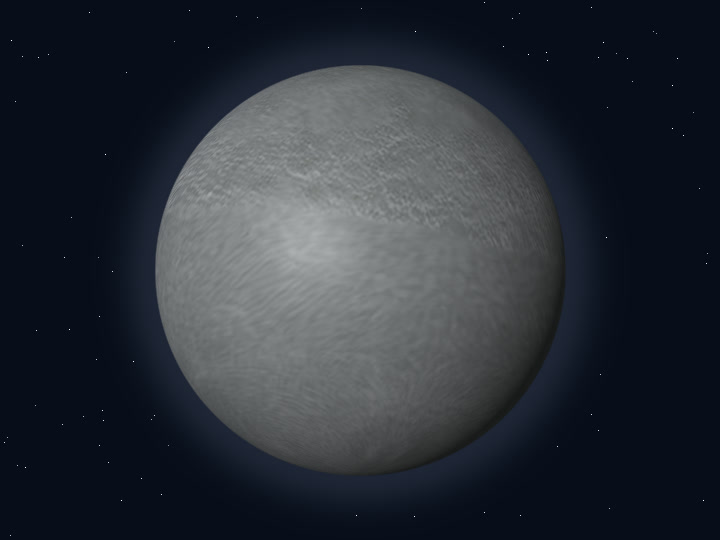
\includegraphics[width=\linewidth,height=4.4cm,keepaspectratio]{imagini/globuri/umbriel.jpg}\\[2pt]
{\scriptsize\itshape\color{orbitarMuted} Vedere 3D a corpului ceresc (\textbf{Umbriel})}
&
\centering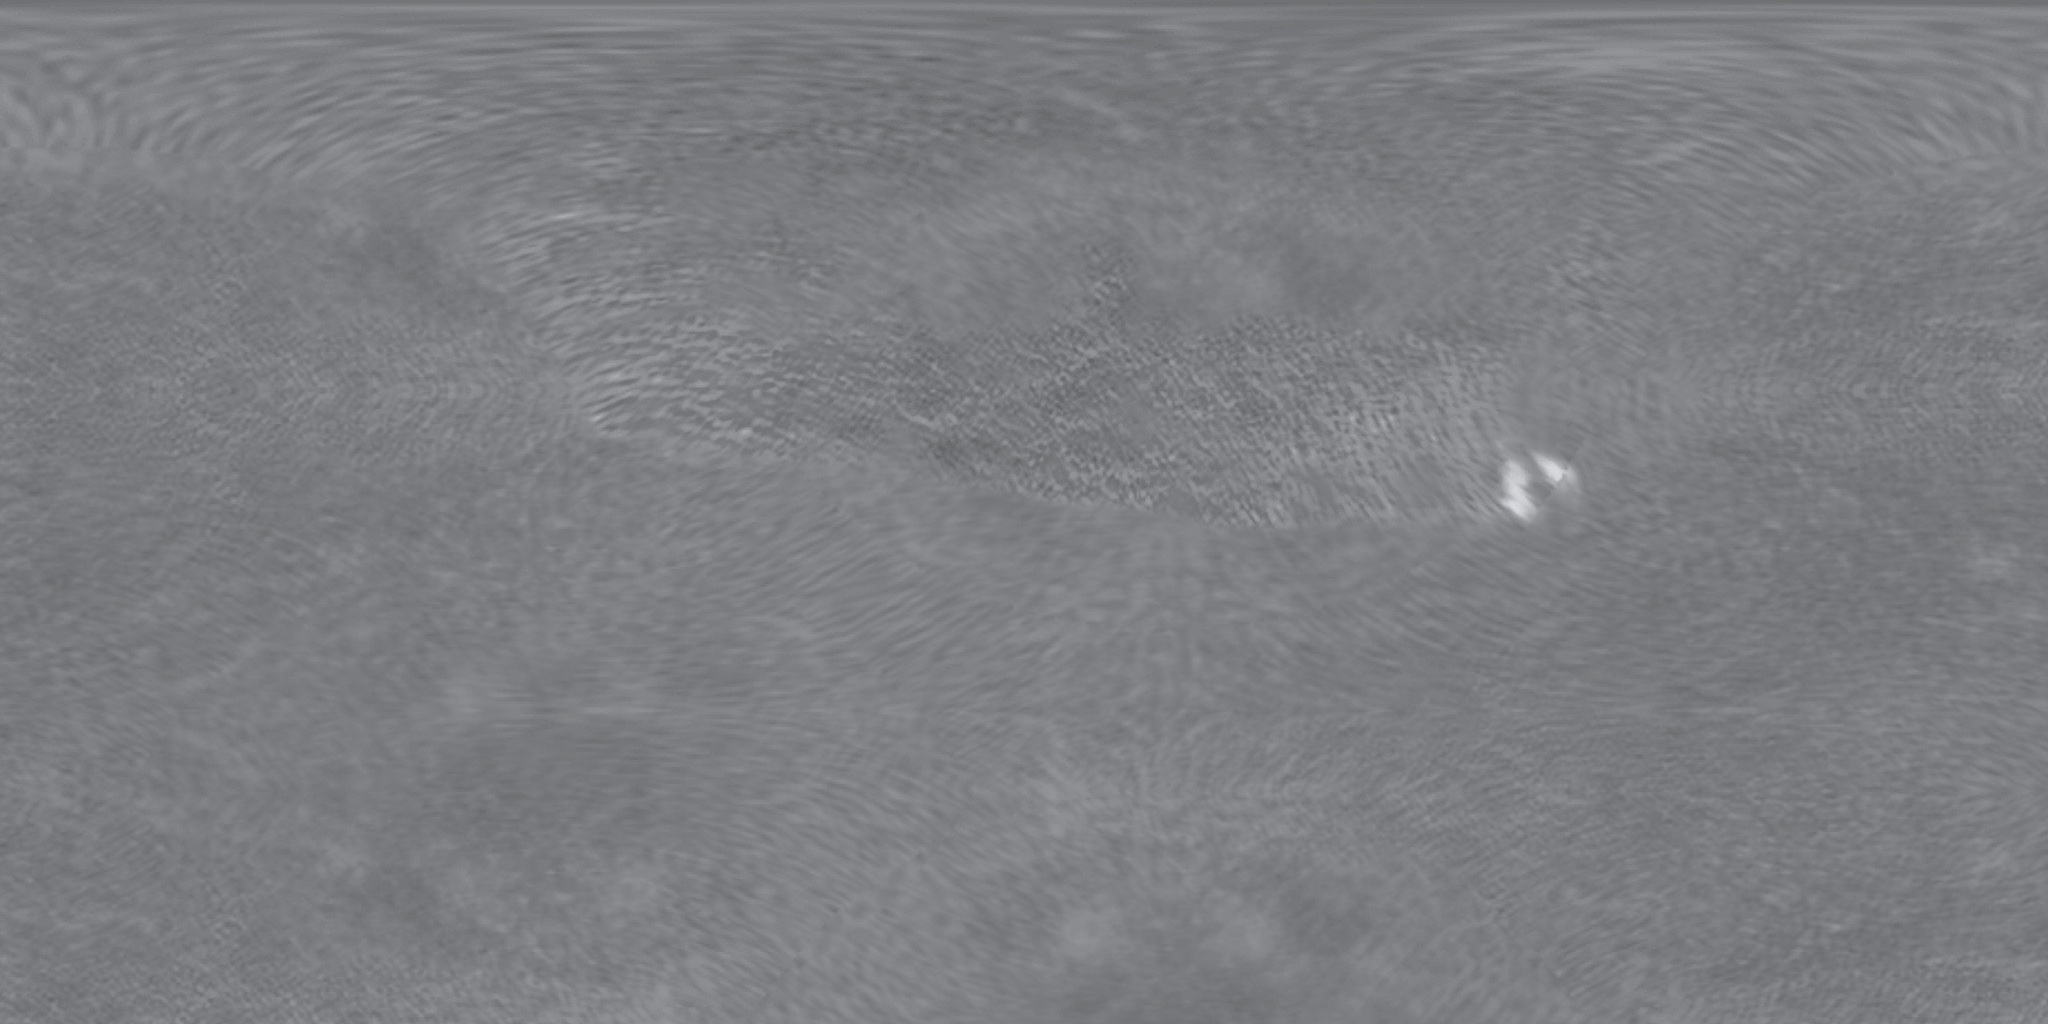
\includegraphics[width=\linewidth,height=4.4cm,keepaspectratio]{../public/textures/hd/umbriel_voyager.jpg}\\[2pt]
{\scriptsize\itshape\color{orbitarMuted} Planiglob desfășurat: Suprafața întunecată a lunii Umbriel și misteriosul inel luminos al craterului Wunda de la ecuator (NASA Voyager 2).}
\end{tabular}
\end{center}


\begin{tcolorbox}[orbitardata, title={\textbf{Repere esențiale: Umbriel}}]
\small
\begin{itemize}[leftmargin=1.4em, itemsep=2pt, topsep=2pt]
  \item \textbf{Clasificare și orbită:} Satelit Natural (Lună) (orbitează în jurul: \textbf{Uranus}) \quad$\bullet$\quad \textbf{Distanță:} 19,218 UA ($\approx$ 2.875 milioane de kilometri)
  \item \textbf{Dimensiuni și masă:} rază medie 584,7 de kilometri \quad$\bullet$\quad masă: 2,13e-4 $\times M_\oplus$
  \item \textbf{Gravitație și regim termic:} 0,023 $\times g_\oplus$ (0,23 m/s$^2$) \quad$\bullet$\quad temperatură medie: -198 $^\circ$C (înclinarea axei: Nespecificată)
  \item \textbf{Ciclu orbital și rotație:} perioadă orbitală (an): 4,144 zile pământești \quad$\bullet$\quad rotație (zi): 99,46 ore (4,14 zile pământești)
  \item \textbf{Durata călătoriei de pe Pământ:} cu viteza luminii ($1c$): \emph{2 ore și 30 de minute}; cu racheta ($50.000$ de kilometri pe oră): \emph{8 ani și jumătate}; cu avionul ($900$ de kilometri pe oră): \emph{345 de ani}; cu mașina ($100$ de kilometri pe oră): \emph{3.100 de ani}.
  \item \textbf{Repere de scară și curiozitate:} Inelul alb din craterul Wunda de pe Umbriel arată din spațiu ca o gogoașă glazurată luminoasă așezată chiar lângă ecuatorul unei lumi întunecate! Numele ei vine de la \guillemotleft{}Umbriel\guillemotright{}, un spirit melancolic al umbrelor dintr-un poem de Alexander Pope (și de la cuvântul latin \guillemotleft{}umbra\guillemotright{}!).
\end{itemize}
\end{tcolorbox}

\subsubsection*{Prezentare generală și profil astrofizic}
Descoperită în 1851 de William Lassell în aceeași zi cu Ariel, Umbriel are aproape aceeași dimensiune (diametru 1.169 de kilometri), dar o istorie geologică complet diferită: reflectă doar 16\% din lumină (jumătate față de Ariel) și păstrează o suprafață străveche, saturată cu cratere mari de impact. Umbriel este cea mai întunecată dintre lunile mari ale lui Uranus! Pe suprafața ei cenușie strălucește ca un far un inel alb misterios, aflat în craterul Wunda. Inelul alb din craterul Wunda de pe Umbriel arată din spațiu ca o gogoașă glazurată luminoasă așezată chiar lângă ecuatorul unei lumi întunecate!

\subsubsection*{Alcătuirea fizică și structura internă}
Privind în profunzimea sa, alcătuirea fizică este organizată pe mai multe straturi și regiuni distincte, fiecare având un rol bine definit în evoluția și dinamica acestui obiect cosmic. În primul rând se remarcă \textbf{Interior de gheață de apă și rocă (1,39 g/cm$^3$)}, care conține o proporție mai mare de gheață și mai puțină rocă decât Ariel, fără semne de refacere tectonică recentă a scoarței. În strânsă legătură cu această componentă se află \textbf{Suprafață străveche întunecată de toline și carbon}, acoperită de un strat subțire de material organic întunecat și cratere de până la 210 kilometri diametru (precum Skynd și Vuver). În completarea acestui ansamblu întâlnim \textbf{Craterul Wunda (131 de kilometri diametru)}, adăpostește pe podeaua sa un inel strălucitor lat de aproximativ 10 kilometri, format probabil din gheață pură de dioxid de carbon (CO$_2$) condensată în capcana termică a craterului.

\subsubsection*{Observații astronomice și istoricul explorării}
Fotografiată de sonda Voyager 2 în ianuarie 1986; este una dintre țintele principale pentru o viitoare sondă orbitală dedicată sistemului Uranus (Uranus Orbiter and Probe). Numele ei vine de la \guillemotleft{}Umbriel\guillemotright{}, un spirit melancolic al umbrelor dintr-un poem de Alexander Pope (și de la cuvântul latin \guillemotleft{}umbra\guillemotright{}!).

\vspace{6pt}
\begin{tcolorbox}[orbitarquiz, title={\textbf{Întrebare de verificare \#27: Umbriel}}]
\textbf{Ce detaliu strălucitor iese în evidență pe suprafața foarte întunecată a satelitului Umbriel?}
\begin{itemize}[leftmargin=2.2em, itemsep=2pt, topsep=4pt]
  \item[$\square$ \textbf{A.}] Inelul alb luminos de pe podeaua craterului ecuatorial Wunda
  \item[$\square$ \textbf{B.}] Un vulcan de sulf
  \item[$\square$ \textbf{C.}] Un ocean de metan lichid
  \item[$\square$ \textbf{D.}] Un inel planetar ca al lui Saturn
\end{itemize}
\vspace{2pt}
{\footnotesize\color{orbitarMuted}\textbf{Răspuns corect:} \textbf{A} (Inelul alb luminos de pe podeaua craterului ecuatorial Wunda). \emph{Craterul Wunda conține un inel lat și foarte luminos (probabil gheață de dioxid de carbon sau gheață de apă curată expusă la impact), care contrastează puternic cu restul suprafeței întunecate a lui Umbriel.}}
\end{tcolorbox}
\clearpage


\subsection{Titania}
\label{sec:body-titania}
\vspace{-4pt}
{\large\itshape\color{orbitarAccent} Cea mai mare lună a planetei Uranus, brăzdată de canioane de gheață}\\[4pt]


\begin{center}
\begin{tabular}{@{}m{0.44\textwidth}@{\hspace{0.03\textwidth}}m{0.51\textwidth}@{}}
\centering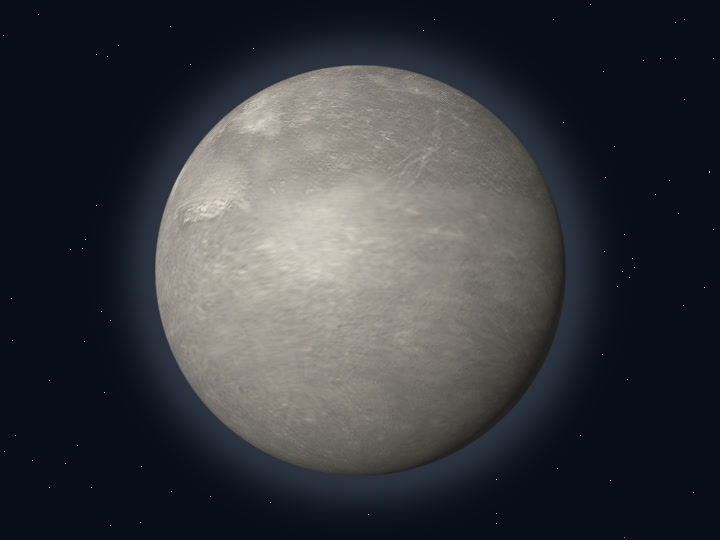
\includegraphics[width=\linewidth,height=4.4cm,keepaspectratio]{imagini/globuri/titania.jpg}\\[2pt]
{\scriptsize\itshape\color{orbitarMuted} Vedere 3D a corpului ceresc (\textbf{Titania})}
&
\centering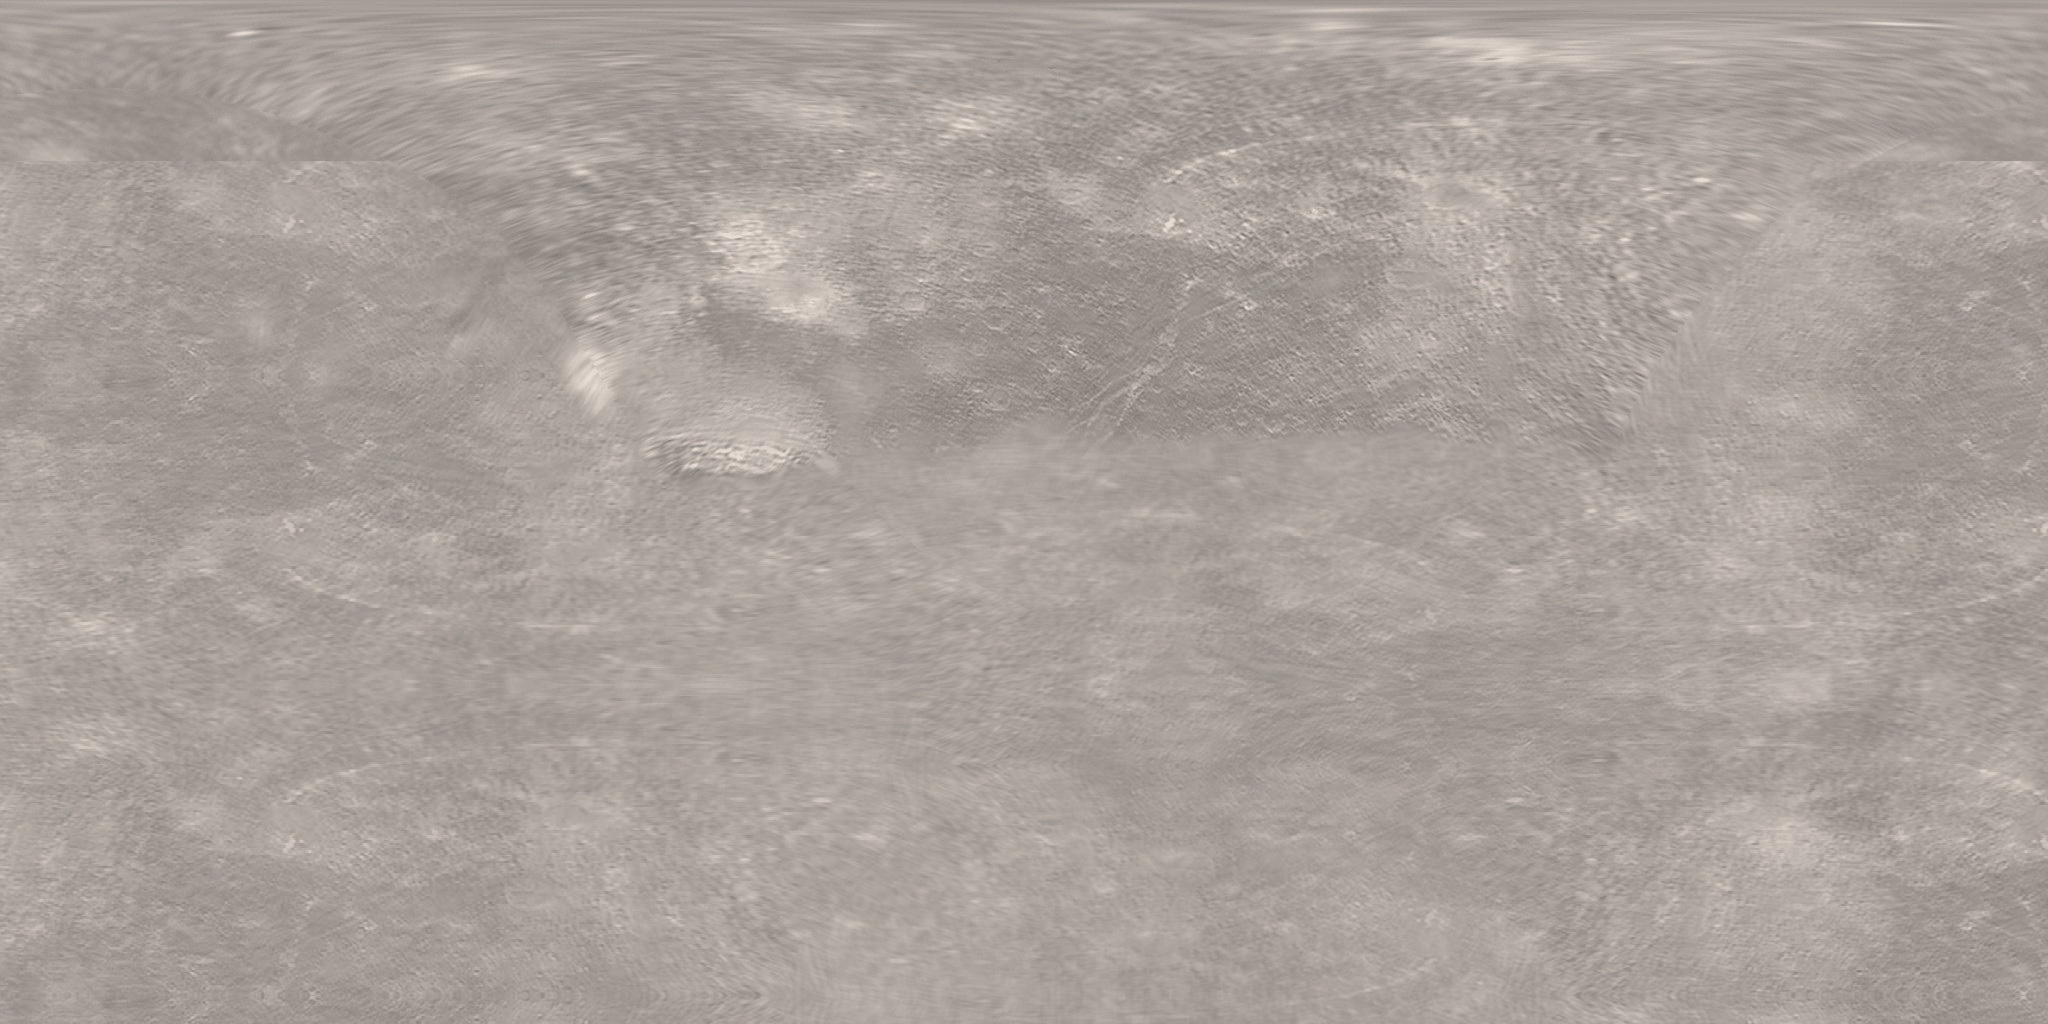
\includegraphics[width=\linewidth,height=4.4cm,keepaspectratio]{../public/textures/hd/titania_voyager.jpg}\\[2pt]
{\scriptsize\itshape\color{orbitarMuted} Planiglob desfășurat: Harta celei mai mari luni a lui Uranus, Titania, și a canionului tectonic Messina Chasmata (NASA Voyager 2).}
\end{tabular}
\end{center}


\begin{tcolorbox}[orbitardata, title={\textbf{Repere esențiale: Titania}}]
\small
\begin{itemize}[leftmargin=1.4em, itemsep=2pt, topsep=2pt]
  \item \textbf{Clasificare și orbită:} Satelit Natural (Lună) (orbitează în jurul: \textbf{Uranus}) \quad$\bullet$\quad \textbf{Distanță:} 19,218 UA ($\approx$ 2.875 milioane de kilometri)
  \item \textbf{Dimensiuni și masă:} rază medie 788,4 de kilometri \quad$\bullet$\quad masă: 5,90e-4 $\times M_\oplus$
  \item \textbf{Gravitație și regim termic:} 0,039 $\times g_\oplus$ (0,38 m/s$^2$) \quad$\bullet$\quad temperatură medie: -203 $^\circ$C (înclinarea axei: Nespecificată)
  \item \textbf{Ciclu orbital și rotație:} perioadă orbitală (an): 8,706 zile pământești \quad$\bullet$\quad rotație (zi): 208,94 ore (8,71 zile pământești)
  \item \textbf{Durata călătoriei de pe Pământ:} cu viteza luminii ($1c$): \emph{2 ore și 30 de minute}; cu racheta ($50.000$ de kilometri pe oră): \emph{8 ani și jumătate}; cu avionul ($900$ de kilometri pe oră): \emph{345 de ani}; cu mașina ($100$ de kilometri pe oră): \emph{3.100 de ani}.
  \item \textbf{Repere de scară și curiozitate:} La fel ca majoritatea sateliților lui Uranus, Titania poartă numele unui personaj din piesele lui William Shakespeare, și anume Regina Zânelor! Canionul Messina Chasmata de pe Titania este atât de lung încât s-ar întinde din România până în Spania!
\end{itemize}
\end{tcolorbox}

\subsubsection*{Prezentare generală și profil astrofizic}
Descoperită de William Herschel în 1787 (în aceeași noapte cu Oberon), Titania este al optulea satelit ca mărime din Sistemul Solar (diametru de 1.578 de kilometri). Orbitează în planul ecuatorial înclinat la 98$^\circ$ al lui Uranus, având anotimpuri extreme de câte 42 de ani. Titania este regina lunilor lui Uranus și cea mai mare dintre ele! Este o lume rece de gheață și stâncă, tăiată de un canion uriaș numit Messina Chasmata. La fel ca majoritatea sateliților lui Uranus, Titania poartă numele unui personaj din piesele lui William Shakespeare, și anume Regina Zânelor!

\subsubsection*{Alcătuirea fizică și structura internă}
Privind în profunzimea sa, alcătuirea fizică este organizată pe mai multe straturi și regiuni distincte, fiecare având un rol bine definit în evoluția și dinamica acestui obiect cosmic. În primul rând se remarcă \textbf{Nucleu stâncos (66\% din rază)}, care conține silicați și compuși organici, reprezentând aproximativ jumătate din masa satelitului. În strânsă legătură cu această componentă se află \textbf{Manta de gheață de apă}, unde când interiorul a înghețat și s-a dilatat în trecut, scoarța a crăpat formând falii gigantice. În completarea acestui ansamblu întâlnim \textbf{Messina Chasmata și Bazinul Gertrude}, sistem de grabene tectonice lung de 1.492 de kilometri și un crater de impact de 326 de kilometri diametru.

\subsubsection*{Observații astronomice și istoricul explorării}
Fotografiată de sonda Voyager 2 în ianuarie 1986; ocultațiile stelare au arătat că poate avea o atmosferă extrem de fină de dioxid de carbon. Canionul Messina Chasmata de pe Titania este atât de lung încât s-ar întinde din România până în Spania!

\vspace{6pt}
\begin{tcolorbox}[orbitarquiz, title={\textbf{Întrebare de verificare \#28: Titania}}]
\textbf{De unde provin numele sateliților planetei Uranus, precum Titania și Miranda?}
\begin{itemize}[leftmargin=2.2em, itemsep=2pt, topsep=4pt]
  \item[$\square$ \textbf{A.}] Din mitologia egipteană
  \item[$\square$ \textbf{B.}] Din operele literare ale lui William Shakespeare și Alexander Pope
  \item[$\square$ \textbf{C.}] De la numele râurilor din Europa
  \item[$\square$ \textbf{D.}] De la numele unor rachete
\end{itemize}
\vspace{2pt}
{\footnotesize\color{orbitarMuted}\textbf{Răspuns corect:} \textbf{B} (Din operele literare ale lui William Shakespeare și Alexander Pope). \emph{Spre deosebire de celelalte planete ale căror luni poartă nume din mitologia greco-romană, lunile lui Uranus sunt numite după personaje din Shakespeare și Pope.}}
\end{tcolorbox}
\clearpage


\subsection{Oberon}
\label{sec:body-oberon}
\vspace{-4pt}
{\large\itshape\color{orbitarAccent} Cea mai exterioară lună mare a lui Uranus, cu craterul Hamlet și un munte de 11 kilometri}\\[4pt]


\begin{center}
\begin{tabular}{@{}m{0.44\textwidth}@{\hspace{0.03\textwidth}}m{0.51\textwidth}@{}}
\centering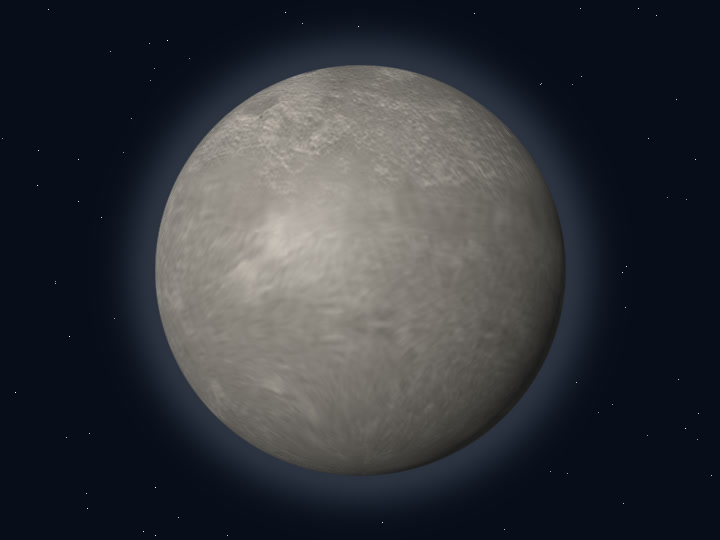
\includegraphics[width=\linewidth,height=4.4cm,keepaspectratio]{imagini/globuri/oberon.jpg}\\[2pt]
{\scriptsize\itshape\color{orbitarMuted} Vedere 3D a corpului ceresc (\textbf{Oberon})}
&
\centering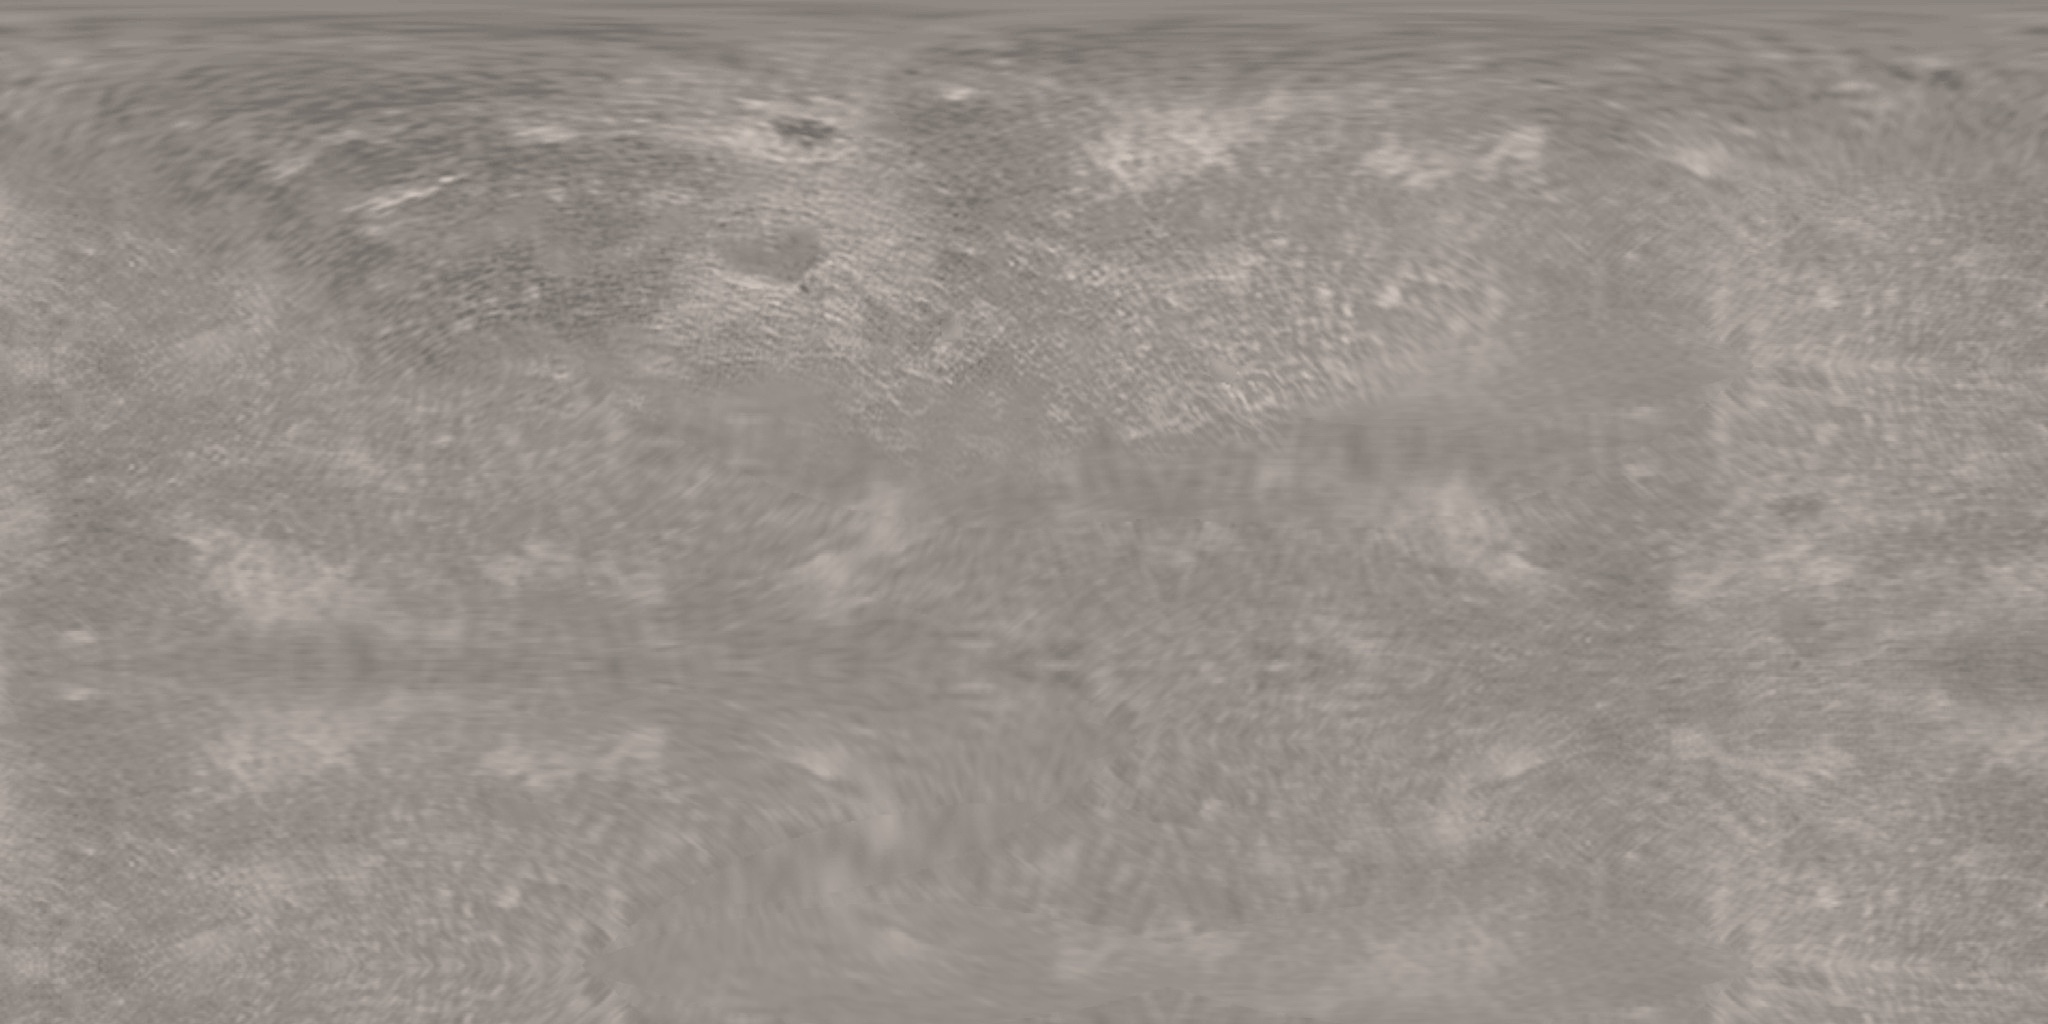
\includegraphics[width=\linewidth,height=4.4cm,keepaspectratio]{../public/textures/hd/oberon_voyager.jpg}\\[2pt]
{\scriptsize\itshape\color{orbitarMuted} Planiglob desfășurat: Harta celei mai exterioare luni mari a lui Uranus, Oberon, cu craterul Hamlet și razele sale de gheață (NASA Voyager 2).}
\end{tabular}
\end{center}


\begin{tcolorbox}[orbitardata, title={\textbf{Repere esențiale: Oberon}}]
\small
\begin{itemize}[leftmargin=1.4em, itemsep=2pt, topsep=2pt]
  \item \textbf{Clasificare și orbită:} Satelit Natural (Lună) (orbitează în jurul: \textbf{Uranus}) \quad$\bullet$\quad \textbf{Distanță:} 19,218 UA ($\approx$ 2.875 milioane de kilometri)
  \item \textbf{Dimensiuni și masă:} rază medie 761,4 de kilometri \quad$\bullet$\quad masă: 5,05e-4 $\times M_\oplus$
  \item \textbf{Gravitație și regim termic:} 0,035 $\times g_\oplus$ (0,34 m/s$^2$) \quad$\bullet$\quad temperatură medie: -198 $^\circ$C (înclinarea axei: Nespecificată)
  \item \textbf{Ciclu orbital și rotație:} perioadă orbitală (an): 13,463 zile pământești \quad$\bullet$\quad rotație (zi): 323,12 ore (13,46 zile pământești)
  \item \textbf{Durata călătoriei de pe Pământ:} cu viteza luminii ($1c$): \emph{2 ore și 30 de minute}; cu racheta ($50.000$ de kilometri pe oră): \emph{8 ani și jumătate}; cu avionul ($900$ de kilometri pe oră): \emph{345 de ani}; cu mașina ($100$ de kilometri pe oră): \emph{3.100 de ani}.
  \item \textbf{Repere de scară și curiozitate:} La marginea globului lui Oberon, sonda Voyager 2 a fotografiat un munte uriaș care se înalță la 11 kilometri deasupra orizontului, fiind mai înalt decât muntele Everest! Multe dintre craterele lui Oberon poartă nume de eroi din piesele lui Shakespeare: Hamlet, Othello, Macbeth, Lear și Romeo!
\end{itemize}
\end{tcolorbox}

\subsubsection*{Prezentare generală și profil astrofizic}
Descoperită de William Herschel la 11 ianuarie 1787 (în aceeași noapte cu Titania), Oberon este al zecelea satelit ca mărime din Sistemul Solar (diametru de 1.522,8 kilometri). Alcătuită în proporții egale din gheață de apă și rocă (densitate 1,63 g/cm$^3$), are o suprafață intens craterizată și canioane tectonice (Mommur Chasma). Oberon este Regele Zânelor și a doua lună ca mărime a lui Uranus! Se rotește cel mai departe de planetă dintre cele cinci luni mari și are cratere cu raze luminoase de gheață. La marginea globului lui Oberon, sonda Voyager 2 a fotografiat un munte uriaș care se înalță la 11 kilometri deasupra orizontului, fiind mai înalt decât muntele Everest!

\subsubsection*{Alcătuirea fizică și structura internă}
Privind în profunzimea sa, alcătuirea fizică este organizată pe mai multe straturi și regiuni distincte, fiecare având un rol bine definit în evoluția și dinamica acestui obiect cosmic. În primul rând se remarcă \textbf{Nucleu stâncos și manta de gheață (50\% rocă, 50\% gheață)}, care poate păstra la limita dintre nucleu și manta un strat subțire de ocean lichid bogat în amoniac. În strânsă legătură cu această componentă se află \textbf{Craterul Hamlet (206 kilometri diametru) și Othello}, cratere mari de impact înconjurate de raze luminoase de gheață proaspătă, dar având podeaua acoperită cu material criovulcanic întunecat. În completarea acestui ansamblu întâlnim \textbf{Muntele de la limb (aproximativ 11 kilometri înălțime) și Mommur Chasma}, un pisc central colosal observat în profil pe marginea discului de Voyager 2 și un canion tectonic lung de 537 de kilometri.

\subsubsection*{Observații astronomice și istoricul explorării}
Fotografiată de sonda Voyager 2 în ianuarie 1986 de la o distanță de 470.600 de kilometri. Multe dintre craterele lui Oberon poartă nume de eroi din piesele lui Shakespeare: Hamlet, Othello, Macbeth, Lear și Romeo!

\vspace{6pt}
\begin{tcolorbox}[orbitarquiz, title={\textbf{Întrebare de verificare \#29: Oberon}}]
\textbf{Ce formațiune spectaculoasă a observat sonda Voyager 2 ridicându-se pe marginea orizontului (limbul) satelitului Oberon?}
\begin{itemize}[leftmargin=2.2em, itemsep=2pt, topsep=4pt]
  \item[$\square$ \textbf{A.}] Un munte de aproximativ 11 kilometri înălțime (probabil piscul central al unui mare bazin de impact)
  \item[$\square$ \textbf{B.}] Un ocean de apă caldă
  \item[$\square$ \textbf{C.}] Un inel de praf
  \item[$\square$ \textbf{D.}] O furtună de nisip
\end{itemize}
\vspace{2pt}
{\footnotesize\color{orbitarMuted}\textbf{Răspuns corect:} \textbf{A} (Un munte de aproximativ 11 kilometri înălțime (probabil piscul central al unui mare bazin de impact)). \emph{În imaginile Voyager 2, pe limbul sud-estic al lui Oberon se profilează un munte înalt de aproximativ 11 kilometri, mai înalt decât Everestul de pe Pământ.}}
\end{tcolorbox}
\clearpage


\section{Neptun}
\label{sec:body-neptune}
\vspace{-4pt}
{\large\itshape\color{orbitarAccent} Planeta albastră a vânturilor supersonice}\\[4pt]


\begin{center}
\begin{tabular}{@{}m{0.44\textwidth}@{\hspace{0.03\textwidth}}m{0.51\textwidth}@{}}
\centering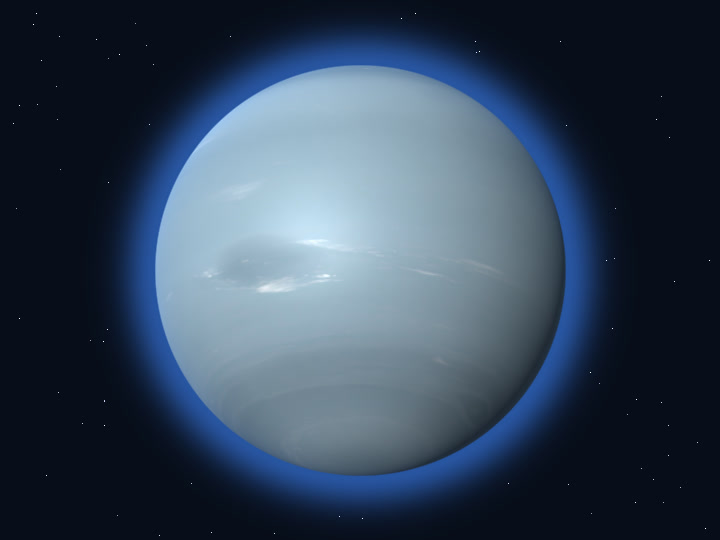
\includegraphics[width=\linewidth,height=4.4cm,keepaspectratio]{imagini/globuri/neptune.jpg}\\[2pt]
{\scriptsize\itshape\color{orbitarMuted} Vedere 3D a corpului ceresc (\textbf{Neptun})}
&
\centering
\includegraphics[width=\linewidth,height=4.4cm,keepaspectratio]{../public/textures/hd/neptune_voyager.jpg}\\[2pt]
{\scriptsize\itshape\color{orbitarMuted} Planiglob desfășurat: Harta atmosferei azurii și a furtunilor supersonice de pe Neptun, cartografiată de NASA Voyager 2.}
\end{tabular}
\end{center}


\begin{tcolorbox}[orbitardata, title={\textbf{Repere esențiale: Neptun}}]
\small
\begin{itemize}[leftmargin=1.4em, itemsep=2pt, topsep=2pt]
  \item \textbf{Clasificare și orbită:} Gigant de Gheață \quad$\bullet$\quad \textbf{Distanță:} 30,110 UA ($\approx$ 4.504 milioane de kilometri)
  \item \textbf{Dimensiuni și masă:} rază medie 24.622 de kilometri \quad$\bullet$\quad masă: 17,150 $\times M_\oplus$
  \item \textbf{Gravitație și regim termic:} 1,140 $\times g_\oplus$ (11,18 m/s$^2$) \quad$\bullet$\quad temperatură medie: -200 $^\circ$C (înclinarea axei: 28,32$^\circ$)
  \item \textbf{Ciclu orbital și rotație:} perioadă orbitală (an): 60.182 zile ($\approx$ 164,77 ani pământești) \quad$\bullet$\quad rotație (zi): 16,11 ore (0,67 zile pământești)
  \item \textbf{Durata călătoriei de pe Pământ:} cu viteza luminii ($1c$): \emph{4 ore și 10 minute}; cu racheta ($50.000$ de kilometri pe oră): \emph{12 ani (Voyager 2)}; cu avionul ($900$ de kilometri pe oră): \emph{550 de ani}; cu mașina ($100$ de kilometri pe oră): \emph{4.950 de ani}.
  \item \textbf{Repere de scară și curiozitate:} Neptun este de 30 de ori mai departe de Soare decât Pământul, astfel că acolo Soarele pare doar o stea foarte strălucitoare! De când a fost descoperit în anul 1846, Neptun a reușit să facă o singură tură completă în jurul Soarelui (în 2011)!
\end{itemize}
\end{tcolorbox}

\subsubsection*{Prezentare generală și profil astrofizic}
Neptun a fost prima planetă a cărei existență a fost prezisă prin calcul matematic (Urbain Le Verrier și John Couch Adams) înainte de a fi observată prin telescop în 1846. Deși primește de 900 de ori mai puțină energie solară decât Pământul, are cea mai dinamică meteorologie dintre giganți. Neptun este cea mai îndepărtată planetă mare de la Soare! Are culoarea unui ocean adânc și vânturi atât de rapide încât depășesc viteza sunetului. Neptun este de 30 de ori mai departe de Soare decât Pământul, astfel că acolo Soarele pare doar o stea foarte strălucitoare!

\subsubsection*{Alcătuirea fizică și structura internă}
Privind în profunzimea sa, alcătuirea fizică este organizată pe mai multe straturi și regiuni distincte, fiecare având un rol bine definit în evoluția și dinamica acestui obiect cosmic. În primul rând se remarcă \textbf{Nucleu stâncos}, cu o masă apropiată de cea a Pământului, la temperaturi de aproximativ 5.000 $^\circ$C. În strânsă legătură cu această componentă se află \textbf{Manta ionică de apă, amoniac și metan}, unde la adâncimi mari, presiunea poate descompune metanul în cristale de diamant. În completarea acestui ansamblu întâlnim \textbf{Atmosferă dinamică}, nori înalți de metan înghețat și vânturi care ating 2.100 kilometri pe oră.

\subsubsection*{Observații astronomice și istoricul explorării}
Survolată de sonda Voyager 2 în august 1989 și observată în infraroșu de Telescopul Spațial James Webb. De când a fost descoperit în anul 1846, Neptun a reușit să facă o singură tură completă în jurul Soarelui (în 2011)!

\vspace{6pt}
\begin{tcolorbox}[orbitarquiz, title={\textbf{Întrebare de verificare \#30: Neptun}}]
\textbf{Cum a fost descoperită planeta Neptun în anul 1846?}
\begin{itemize}[leftmargin=2.2em, itemsep=2pt, topsep=4pt]
  \item[$\square$ \textbf{A.}] Cu ochiul liber în Antichitate
  \item[$\square$ \textbf{B.}] Prin calcule matematice bazate pe perturbațiile orbitei lui Uranus
  \item[$\square$ \textbf{C.}] De către sonda Voyager 2
  \item[$\square$ \textbf{D.}] În timpul unei eclipse solare
\end{itemize}
\vspace{2pt}
{\footnotesize\color{orbitarMuted}\textbf{Răspuns corect:} \textbf{B} (Prin calcule matematice bazate pe perturbațiile orbitei lui Uranus). \emph{Matematicienii au observat că Uranus nu urma exact orbita calculată și au dedus poziția unei planete necunoscute care îl atrăgea gravitațional.}}
\end{tcolorbox}
\clearpage


\subsection{Triton}
\label{sec:body-triton}
\vspace{-4pt}
{\large\itshape\color{orbitarAccent} Marea lună înghețată a lui Neptun, cu gheizere de azot și orbită inversă}\\[4pt]


\begin{center}
\begin{tabular}{@{}m{0.44\textwidth}@{\hspace{0.03\textwidth}}m{0.51\textwidth}@{}}
\centering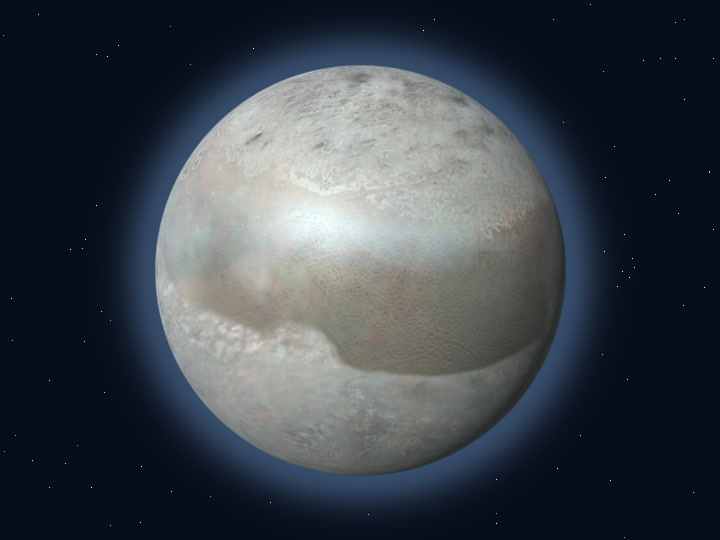
\includegraphics[width=\linewidth,height=4.4cm,keepaspectratio]{imagini/globuri/triton.jpg}\\[2pt]
{\scriptsize\itshape\color{orbitarMuted} Vedere 3D a corpului ceresc (\textbf{Triton})}
&
\centering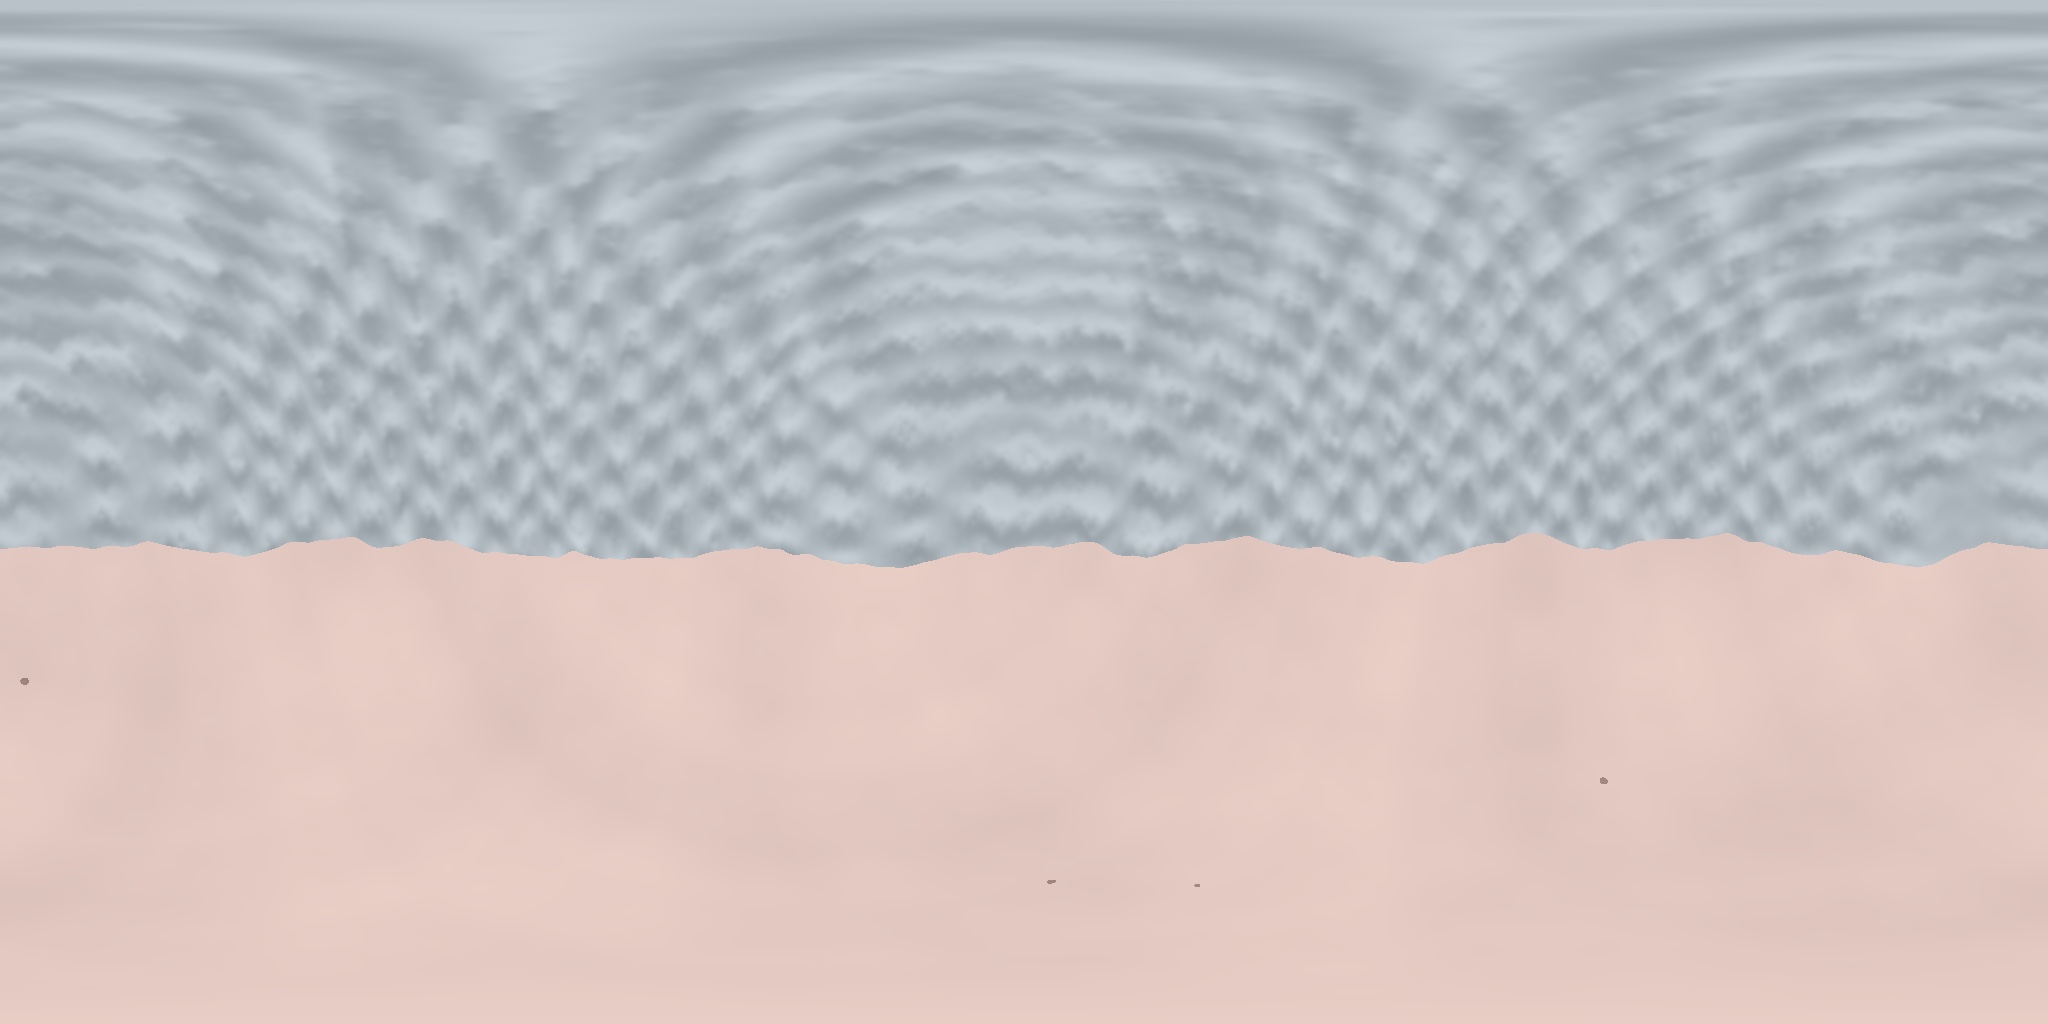
\includegraphics[width=\linewidth,height=4.4cm,keepaspectratio]{../public/textures/hd/triton_voyager.jpg}\\[2pt]
{\scriptsize\itshape\color{orbitarMuted} Planiglob desfășurat: Terenul de tip \quotedblbase{}coajă de pepene galben\textquotedblright{} și calota de azot înghețat cu gheizere de pe Triton (NASA Voyager 2).}
\end{tabular}
\end{center}


\begin{tcolorbox}[orbitardata, title={\textbf{Repere esențiale: Triton}}]
\small
\begin{itemize}[leftmargin=1.4em, itemsep=2pt, topsep=2pt]
  \item \textbf{Clasificare și orbită:} Satelit Natural (Lună) (orbitează în jurul: \textbf{Neptun}) \quad$\bullet$\quad \textbf{Distanță:} 30,110 UA ($\approx$ 4.504 milioane de kilometri)
  \item \textbf{Dimensiuni și masă:} rază medie 1.353,4 de kilometri \quad$\bullet$\quad masă: 0,004 $\times M_\oplus$
  \item \textbf{Gravitație și regim termic:} 0,079 $\times g_\oplus$ (0,77 m/s$^2$) \quad$\bullet$\quad temperatură medie: -235 $^\circ$C (înclinarea axei: Nespecificată)
  \item \textbf{Ciclu orbital și rotație:} perioadă orbitală (an): 5,877 zile pământești (Orbită retrogradă!) \quad$\bullet$\quad rotație (zi): 141,00 ore (Rotație retrogradă!)
  \item \textbf{Durata călătoriei de pe Pământ:} cu viteza luminii ($1c$): \emph{4 ore și 10 minute}; cu racheta ($50.000$ de kilometri pe oră): \emph{12 ani (Voyager 2)}; cu avionul ($900$ de kilometri pe oră): \emph{550 de ani}; cu mașina ($100$ de kilometri pe oră): \emph{4.950 de ani}.
  \item \textbf{Repere de scară și curiozitate:} O mare parte din suprafața lui Triton are denivelări ciudate care arată exact ca coaja unui pepene galben! Triton este singura lună mare din Sistemul Solar care merge \guillemotleft{}pe contrasens\guillemotright{} și se învârte în jurul lui Neptun în sens invers față de rotația planetei!
\end{itemize}
\end{tcolorbox}

\subsubsection*{Prezentare generală și profil astrofizic}
Descoperită în 1846 de William Lassell la doar 17 zile după descoperirea lui Neptun, Triton este al șaptelea satelit ca mărime din Sistemul Solar (mai mare decât Pluto). Orbita sa retrogradă demonstrează că a fost o planetă pitică din Centura Kuiper capturată gravitațional de Neptun. Triton este cea mai mare lună a lui Neptun și una dintre cele mai reci lumi din Sistemul Solar! Are gheizere care aruncă nori negri de azot înghețat până la 8 kilometri înălțime. O mare parte din suprafața lui Triton are denivelări ciudate care arată exact ca coaja unui pepene galben!

\subsubsection*{Alcătuirea fizică și structura internă}
Privind în profunzimea sa, alcătuirea fizică este organizată pe mai multe straturi și regiuni distincte, fiecare având un rol bine definit în evoluția și dinamica acestui obiect cosmic. În primul rând se remarcă \textbf{Nucleu mare stâncos-metalic}, densitate ridicată (2,06 g/cm$^3$) și posibil ocean subglaciar menținut lichid de căldura radiogenică și mareică. În strânsă legătură cu această componentă se află \textbf{Teren \guillemotleft{}coajă de pepene galben\guillemotright{} (Bubembe Regio)}, regiune unică formată prin diapirismul gheții (ridicarea și coborârea lentă a blocurilor de gheață). În completarea acestui ansamblu întâlnim \textbf{Calotă polară rozalie de azot și criovulcani}, gheizere active de azot gazos și praf întunecat, plus o atmosferă subțire de azot cu nori la 235 $^\circ$C sub zero.

\subsubsection*{Observații astronomice și istoricul explorării}
Explorată în premieră la 25 august 1989 de sonda Voyager 2, care a fotografiat în direct erupțiile gheizerelor sale polare. Triton este singura lună mare din Sistemul Solar care merge \guillemotleft{}pe contrasens\guillemotright{} și se învârte în jurul lui Neptun în sens invers față de rotația planetei!

\vspace{6pt}
\begin{tcolorbox}[orbitarquiz, title={\textbf{Întrebare de verificare \#31: Triton}}]
\textbf{Ce ne indică faptul că satelitul Triton se rotește în sens invers (retrograd) în jurul lui Neptun?}
\begin{itemize}[leftmargin=2.2em, itemsep=2pt, topsep=4pt]
  \item[$\square$ \textbf{A.}] Că nu s-a format lângă Neptun, ci a fost un corp din Centura Kuiper capturat de gravitația planetei
  \item[$\square$ \textbf{B.}] Că Neptun nu are gravitație
  \item[$\square$ \textbf{C.}] Că este făcut din fier
  \item[$\square$ \textbf{D.}] Că se îndepărtează de Soare
\end{itemize}
\vspace{2pt}
{\footnotesize\color{orbitarMuted}\textbf{Răspuns corect:} \textbf{A} (Că nu s-a format lângă Neptun, ci a fost un corp din Centura Kuiper capturat de gravitația planetei). \emph{Un satelit format împreună cu planeta sa orbitează în sensul rotației planetei; orbita retrogradă a lui Triton dovedește că a fost capturat din Centura Kuiper.}}
\end{tcolorbox}
\clearpage


% SPDX-License-Identifier: GPL-3.0-or-later
\chapter{Centuri Cosmice, Planete Pitice și Asteroizi}
\label{chap:corpuri-sistem-solar}

Dincolo de cele 8 planete majore și sateliții lor naturali prezentați în Capitolul~\ref{chap:planete}, Sistemul Solar adăpostește \textbf{două centuri uriașe de corpuri minore} (Centura Principală de Asteroizi și Centura Kuiper), \textbf{5 planete pitice recunoscute de Uniunea Astronomică Internațională} (împreună cu satelitul binar \textbf{Charon}, asociat planetei pitice \textbf{Pluto}) și \textbf{5 asteroizi emblematici}.

\section{Centura Principală de Asteroizi și Centura Kuiper}
\label{sec:centuri}

În \textbf{Orbitar}, mii de corpuri stâncoase și înghețate sunt simulate simultan în timp real în cele două mari centuri circumsolare:


\subsection{Centura Principală de Asteroizi}
\begin{tcolorbox}[orbitardata, title={\textbf{Parametrii Regiunii Toroidale — Centura Principală de Asteroizi}}]
\begin{tabularx}{\textwidth}{@{}lX@{}}
\textbf{Rază interioară -- exterioară} & 2,15 UA -- 3,25 UA față de Soare \\
\textbf{Grosime verticală în modelul 3D} & 0,35 UA (2.200 asteroizi/corpuri randate prin \texttt{THREE.InstancedMesh}) \\
\textbf{Descriere științifică} & Regiune toroidală între orbitele planetelor Marte și Jupiter, populată de milioane de corpuri stâncoase și metalice rămase de la formarea Sistemului Solar. \\
\end{tabularx}
\end{tcolorbox}


\subsection{Centura Kuiper}
\begin{tcolorbox}[orbitardata, title={\textbf{Parametrii Regiunii Toroidale — Centura Kuiper}}]
\begin{tabularx}{\textwidth}{@{}lX@{}}
\textbf{Rază interioară -- exterioară} & 30,50 UA -- 49,00 UA față de Soare \\
\textbf{Grosime verticală în modelul 3D} & 3,20 UA (2.800 asteroizi/corpuri randate prin \texttt{THREE.InstancedMesh}) \\
\textbf{Descriere științifică} & Disc vast de corpuri înghețate situat dincolo de orbita lui Neptun, casa planetelor pitice Pluto, Haumea și Makemake. \\
\end{tabularx}
\end{tcolorbox}


\begin{tcolorbox}[orbitarjunior, title={\textbf{Mit vs. Realitate: Cum arată în realitate zborul printr-o centură de asteroizi?}}]
În filmele SF, navele spațiale trebuie să facă slalom periculos printre stânci uriașe înghesuite unele lângă altele. \textbf{În realitate}, Centura de Asteroizi și Centura Kuiper sunt atât de vaste încât distanța medie dintre doi asteroizi de dimensiuni notabile este de \textbf{sute de mii sau milioane de kilometri} (de câteva ori distanța de la Pământ la Lună!). Toate sondele trimise de NASA și ESA (precum \emph{Pioneer}, \emph{Voyager}, \emph{Galileo}, \emph{Cassini}, \emph{New Horizons} și \emph{JUICE}) au traversat centura fără să lovească absolut nimic!
\end{tcolorbox}

\begin{table}[H]
\centering
\small
\caption{Planetele pitice și asteroizii principali din Orbitar}
\resizebox{\textwidth}{!}{%
\begin{tabular}{@{}llrrrr@{}}
\toprule
\textbf{Nume} & \textbf{Categorie} & \textbf{Distanță Soare} & \textbf{Rază medie (km)} & \textbf{Perioadă orbitală} & \textbf{Temp. medie} \\
\midrule
Ceres & Planetă pitică & 2,77 UA & 473,00 & 4,61 ani & -105$^\circ$C \\
Pluto & Planetă pitică & 39,48 UA & 1188,30 & 247,94 ani & -229$^\circ$C \\
Haumea & Planetă pitică & 43,13 UA & 780,00 & 284,12 ani & -241$^\circ$C \\
Makemake & Planetă pitică & 45,43 UA & 715,00 & 306,21 ani & -243$^\circ$C \\
Eris & Planetă pitică & 67,86 UA & 1163,00 & 558,06 ani & -243$^\circ$C \\
4 Vesta & Asteroid & 2,36 UA & 262,70 & 3,63 ani & -60$^\circ$C \\
2 Pallas & Asteroid & 2,77 UA & 256,00 & 4,62 ani & -109$^\circ$C \\
16 Psyche & Asteroid & 2,92 UA & 111,00 & 4,99 ani & -100$^\circ$C \\
101955 Bennu & Asteroid & 1,13 UA & 0,24 & 1,20 ani & 4$^\circ$C \\
99942 Apophis & Asteroid & 0,92 UA & 0,18 & 0,89 ani & 17$^\circ$C \\
\bottomrule
\end{tabular}%
}
\end{table}

\clearpage
\section{Cele 5 Planete Pitice și Sistemul Binar Pluto--Charon}

\subsection{Ceres}
\label{sec:body-ceres}
\vspace{-4pt}
{\large\itshape\color{orbitarAccent} Singura planetă pitică din Centura Principală de Asteroizi}\\[4pt]


\begin{center}
\begin{tabular}{@{}m{0.44\textwidth}@{\hspace{0.03\textwidth}}m{0.51\textwidth}@{}}
\centering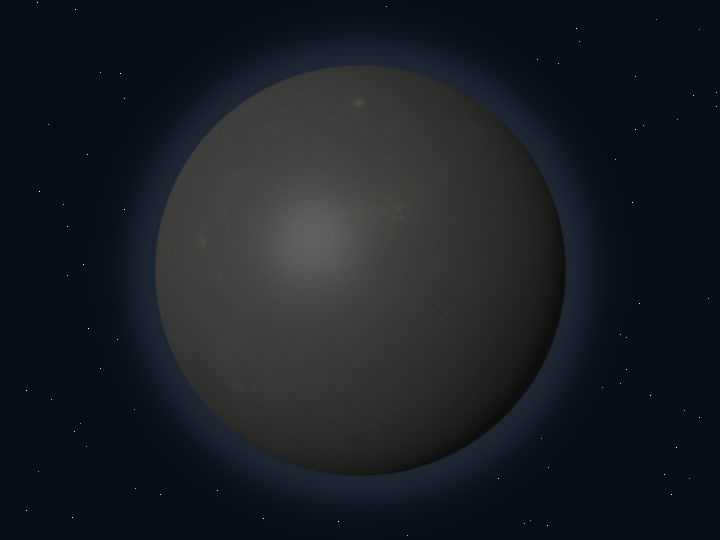
\includegraphics[width=\linewidth,height=4.4cm,keepaspectratio]{imagini/globuri/ceres.jpg}\\[2pt]
{\scriptsize\itshape\color{orbitarMuted} Vedere 3D a corpului ceresc (\textbf{Ceres})}
&
\centering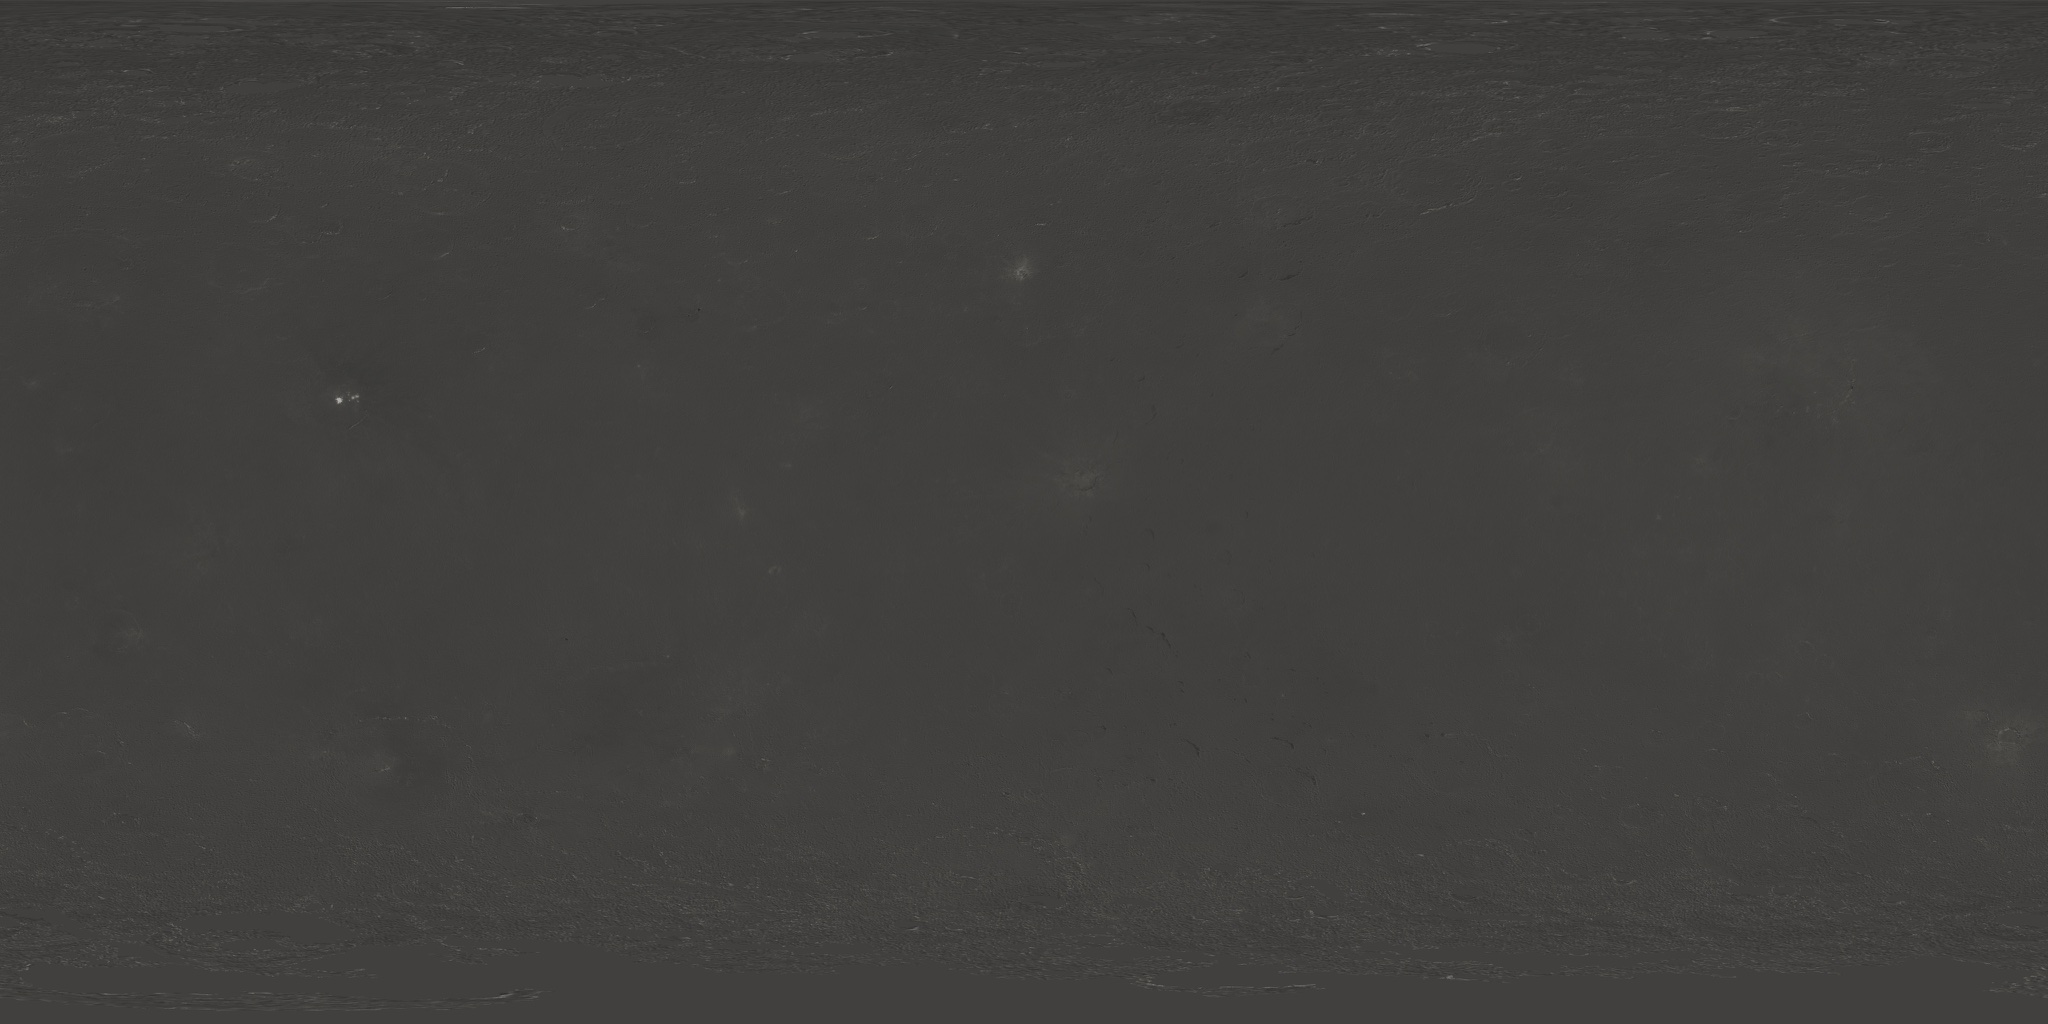
\includegraphics[width=\linewidth,height=4.4cm,keepaspectratio]{../public/textures/hd/ceres_dawn.jpg}\\[2pt]
{\scriptsize\itshape\color{orbitarMuted} Planiglob desfășurat: Harta globală a planetei pitice Ceres și a craterului Occator cu depozite strălucitoare de săruri (sonda NASA Dawn).}
\end{tabular}
\end{center}


\begin{tcolorbox}[orbitardata, title={\textbf{Repere esențiale: Ceres}}]
\small
\begin{itemize}[leftmargin=1.4em, itemsep=2pt, topsep=2pt]
  \item \textbf{Clasificare și orbită:} Planetă Pitică \quad$\bullet$\quad \textbf{Distanță:} 2,767 UA ($\approx$ 414 milioane de kilometri)
  \item \textbf{Dimensiuni și masă:} rază medie 473 de kilometri \quad$\bullet$\quad masă: 1,50e-4 $\times M_\oplus$
  \item \textbf{Gravitație și regim termic:} 0,029 $\times g_\oplus$ (0,28 m/s$^2$) \quad$\bullet$\quad temperatură medie: -105 $^\circ$C (înclinarea axei: Nespecificată)
  \item \textbf{Ciclu orbital și rotație:} perioadă orbitală (an): 1.682 zile ($\approx$ 4,61 ani pământești) \quad$\bullet$\quad rotație (zi): 9,07 ore (0,38 zile pământești) (elemente kepleriene: $a = 2,767$ UA, $e = 0,0760$, $i = 10,59^\circ$, $\Omega = 80,3^\circ$, $\omega = 73,6^\circ$)
  \item \textbf{Durata călătoriei de pe Pământ:} cu viteza luminii ($1c$): \emph{22 de minute}; cu racheta ($50.000$ de kilometri pe oră): \emph{1,5--3 ani}; cu avionul ($900$ de kilometri pe oră): \emph{33 de ani}; cu mașina ($100$ de kilometri pe oră): \emph{300 de ani}.
  \item \textbf{Repere de scară și curiozitate:} Dacă toți asteroizii din centură ar fi adunați într-o găleată, Ceres singură ar umple o treime din găleată! În craterul Occator de pe Ceres strălucesc pete albe misterioase, făcute din sare lăsată în urmă de izvoare sărate!
\end{itemize}
\end{tcolorbox}

\subsubsection*{Prezentare generală și profil astrofizic}
Descoperită la 1 ianuarie 1801 de Giuseppe Piazzi, Ceres este singura planetă pitică situată în Sistemul Solar interior. Reprezintă o protoplanetă embrionară bogată în apă și argile amoniacale. Ceres este cea mai mare lume din Centura de Asteroizi dintre Marte și Jupiter! Este atât de mare încât propria ei gravitație a modelat-o într-o sferă. Dacă toți asteroizii din centură ar fi adunați într-o găleată, Ceres singură ar umple o treime din găleată!

\subsubsection*{Alcătuirea fizică și structura internă}
Privind în profunzimea sa, alcătuirea fizică este organizată pe mai multe straturi și regiuni distincte, fiecare având un rol bine definit în evoluția și dinamica acestui obiect cosmic. În primul rând se remarcă \textbf{Nucleu stâncos hidratat}, compus din silicați și minerale argiloase. În strânsă legătură cu această componentă se află \textbf{Manta bogată în gheață și saramură}, rezervoare subterane de apă sărată care alimentează criovulcanismul (ex. muntele Ahuna Mons). În completarea acestui ansamblu întâlnim \textbf{Crustă întunecată cu depozite de carbonat de sodiu}, unde petele luminoase (faculae) din craterul Occator sunt depozite de săruri hidrotermale.

\subsubsection*{Observații astronomice și istoricul explorării}
A fost prima planetă pitică vizitată și orbitată de o sondă spațială: misiunea NASA Dawn (2015--2018). În craterul Occator de pe Ceres strălucesc pete albe misterioase, făcute din sare lăsată în urmă de izvoare sărate!

\vspace{6pt}
\begin{tcolorbox}[orbitarquiz, title={\textbf{Întrebare de verificare \#32: Ceres}}]
\textbf{Unde se află planeta pitică Ceres?}
\begin{itemize}[leftmargin=2.2em, itemsep=2pt, topsep=4pt]
  \item[$\square$ \textbf{A.}] Dincolo de Neptun, în Centura Kuiper
  \item[$\square$ \textbf{B.}] În Centura Principală de Asteroizi, între Marte și Jupiter
  \item[$\square$ \textbf{C.}] Pe orbita Pământului
  \item[$\square$ \textbf{D.}] Între Mercur și Venus
\end{itemize}
\vspace{2pt}
{\footnotesize\color{orbitarMuted}\textbf{Răspuns corect:} \textbf{B} (În Centura Principală de Asteroizi, între Marte și Jupiter). \emph{Ceres orbitează la 2,77 UA de Soare, în mijlocul Centurii Principale de Asteroizi dintre Marte și Jupiter.}}
\end{tcolorbox}
\clearpage


\subsection{Pluto}
\label{sec:body-pluto}
\vspace{-4pt}
{\large\itshape\color{orbitarAccent} Regele planetelor pitice din Centura Kuiper}\\[4pt]


\begin{center}
\begin{tabular}{@{}m{0.44\textwidth}@{\hspace{0.03\textwidth}}m{0.51\textwidth}@{}}
\centering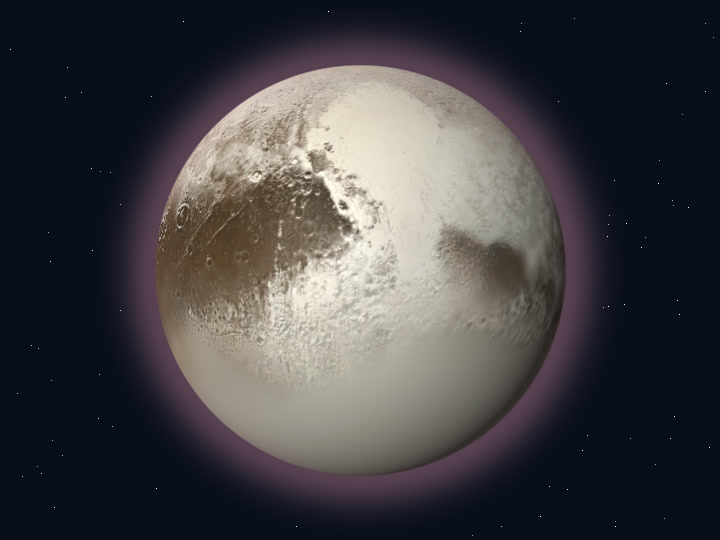
\includegraphics[width=\linewidth,height=4.4cm,keepaspectratio]{imagini/globuri/pluto.jpg}\\[2pt]
{\scriptsize\itshape\color{orbitarMuted} Vedere 3D a corpului ceresc (\textbf{Pluto})}
&
\centering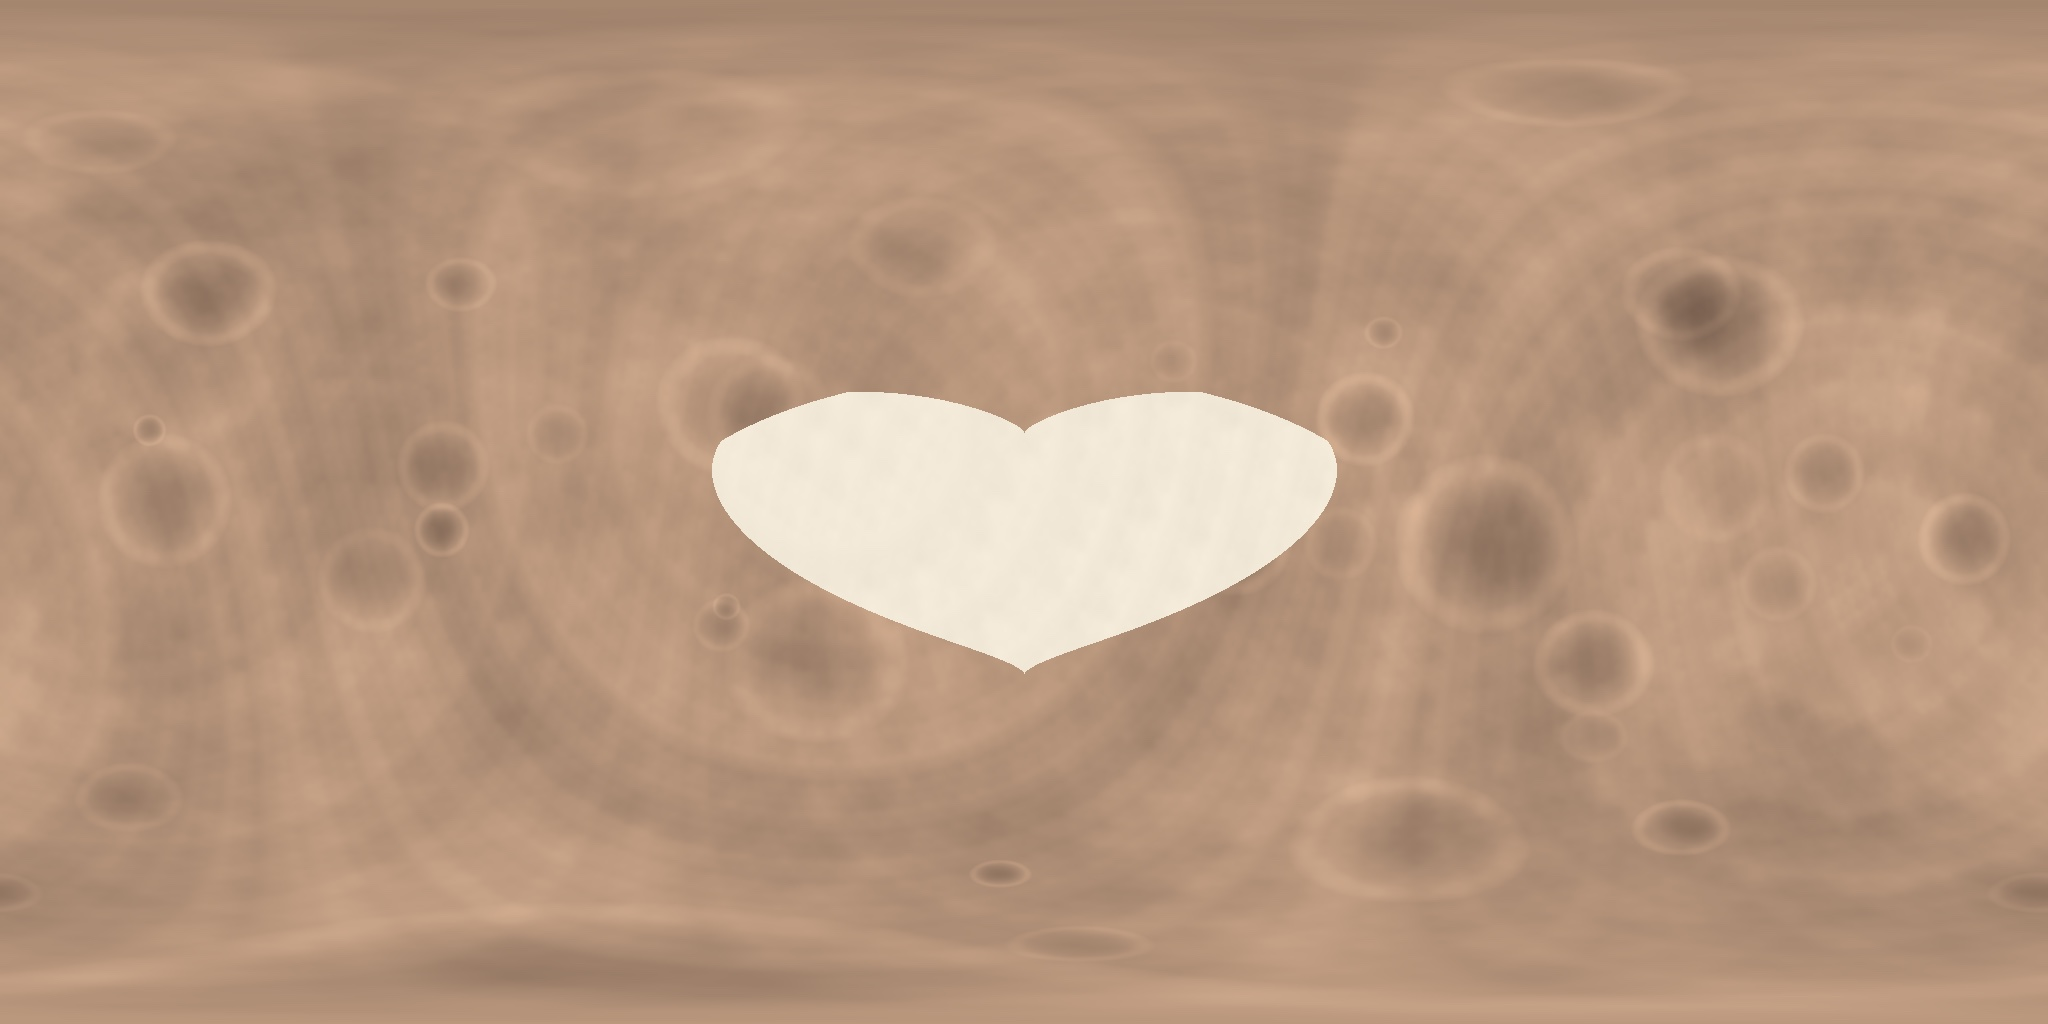
\includegraphics[width=\linewidth,height=4.4cm,keepaspectratio]{../public/textures/hd/pluto_newhorizons.jpg}\\[2pt]
{\scriptsize\itshape\color{orbitarMuted} Planiglob desfășurat: Harta globală a planetei pitice Pluto și a ghețarului în formă de inimă Tombaugh Regio / Sputnik Planitia (NASA New Horizons).}
\end{tabular}
\end{center}


\begin{tcolorbox}[orbitardata, title={\textbf{Repere esențiale: Pluto}}]
\small
\begin{itemize}[leftmargin=1.4em, itemsep=2pt, topsep=2pt]
  \item \textbf{Clasificare și orbită:} Planetă Pitică \quad$\bullet$\quad \textbf{Distanță:} 39,480 UA ($\approx$ 5.906 milioane de kilometri)
  \item \textbf{Dimensiuni și masă:} rază medie 1.188,3 de kilometri \quad$\bullet$\quad masă: 0,002 $\times M_\oplus$
  \item \textbf{Gravitație și regim termic:} 0,063 $\times g_\oplus$ (0,62 m/s$^2$) \quad$\bullet$\quad temperatură medie: -229 $^\circ$C (înclinarea axei: 122,53$^\circ$)
  \item \textbf{Ciclu orbital și rotație:} perioadă orbitală (an): 90.560 zile ($\approx$ 247,94 ani pământești) \quad$\bullet$\quad rotație (zi): 153,30 ore (Rotație retrogradă!)
  \item \textbf{Durata călătoriei de pe Pământ:} cu viteza luminii ($1c$): \emph{5 ore și 30 de minute}; cu racheta ($50.000$ de kilometri pe oră): \emph{9 ani și jumătate (New Horizons)}; cu avionul ($900$ de kilometri pe oră): \emph{720 de ani}; cu mașina ($100$ de kilometri pe oră): \emph{6.500 de ani}.
  \item \textbf{Repere de scară și curiozitate:} Pluto este mai mic chiar și decât Luna noastră, măsurând cam cât jumătate din lățimea Europei! Pluto și satelitul său cel mai mare, Charon, sunt atât de apropiați ca mărime încât dansează unul în jurul celuilalt!
\end{itemize}
\end{tcolorbox}

\subsubsection*{Prezentare generală și profil astrofizic}
Descoperită de Clyde Tombaugh în 1930 și reclasificată în 2006 de UAI drept planetă pitică (obiect plutoid din Centura Kuiper), Pluto are o orbită excentrică și înclinată la 17$^\circ$ și o geologie surprinzător de activă, cu munți de gheață de apă și ghețari de azot. Pluto este o planetă pitică îndepărtată și înghețată care poartă pe pieptul ei o formă uriașă de inimă albă din gheață de azot! Pluto este mai mic chiar și decât Luna noastră, măsurând cam cât jumătate din lățimea Europei!

\subsubsection*{Alcătuirea fizică și structura internă}
Privind în profunzimea sa, alcătuirea fizică este organizată pe mai multe straturi și regiuni distincte, fiecare având un rol bine definit în evoluția și dinamica acestui obiect cosmic. În primul rând se remarcă \textbf{Nucleu stâncos (70\% din diametru)}, bogat în silicați, a cărui dezintegrare radioactivă menține căldura internă. În strânsă legătură cu această componentă se află \textbf{Manta de gheață de apă ( și posibil ocean subteran)}, care susține lanțuri muntoase înalte de 3--4 kilometri. În completarea acestui ansamblu întâlnim \textbf{Suprafață de azot, metan și CO înghețat}, dominată de câmpia convectivă Sputnik Planitia (\guillemotleft{}Inima lui Pluto\guillemotright{}).

\subsubsection*{Observații astronomice și istoricul explorării}
Survolată în premieră istorică la 14 iulie 2015 de sonda NASA New Horizons, care a dezvăluit munți și câmpii de gheață tinere. Pluto și satelitul său cel mai mare, Charon, sunt atât de apropiați ca mărime încât dansează unul în jurul celuilalt!

\vspace{6pt}
\begin{tcolorbox}[orbitarquiz, title={\textbf{Întrebare de verificare \#33: Pluto}}]
\textbf{Cum se numește celebra regiune strălucitoare în formă de inimă de pe Pluto?}
\begin{itemize}[leftmargin=2.2em, itemsep=2pt, topsep=4pt]
  \item[$\square$ \textbf{A.}] Tombaugh Regio (Sputnik Planitia)
  \item[$\square$ \textbf{B.}] Olympus Mons
  \item[$\square$ \textbf{C.}] Mare Tranquillitatis
  \item[$\square$ \textbf{D.}] Caloris Planitia
\end{itemize}
\vspace{2pt}
{\footnotesize\color{orbitarMuted}\textbf{Răspuns corect:} \textbf{A} (Tombaugh Regio (Sputnik Planitia)). \emph{Regiunea în formă de inimă a fost numită Tombaugh Regio în onoarea descoperitorului lui Pluto, iar lobul ei vestic este ghețarul Sputnik Planitia.}}
\end{tcolorbox}
\clearpage


\subsection{Charon}
\label{sec:body-charon}
\vspace{-4pt}
{\large\itshape\color{orbitarAccent} Satelitul-pereche al lui Pluto, cu calota roșiatică Mordor Macula}\\[4pt]


\begin{center}
\begin{tabular}{@{}m{0.44\textwidth}@{\hspace{0.03\textwidth}}m{0.51\textwidth}@{}}
\centering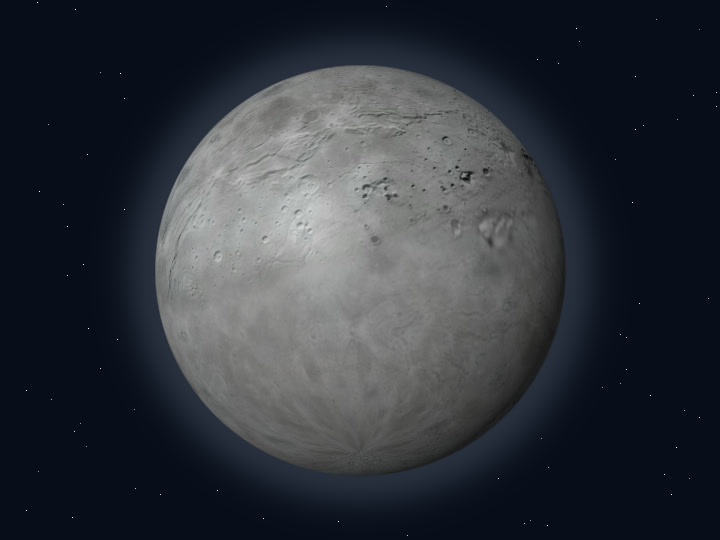
\includegraphics[width=\linewidth,height=4.4cm,keepaspectratio]{imagini/globuri/charon.jpg}\\[2pt]
{\scriptsize\itshape\color{orbitarMuted} Vedere 3D a corpului ceresc (\textbf{Charon})}
&
\centering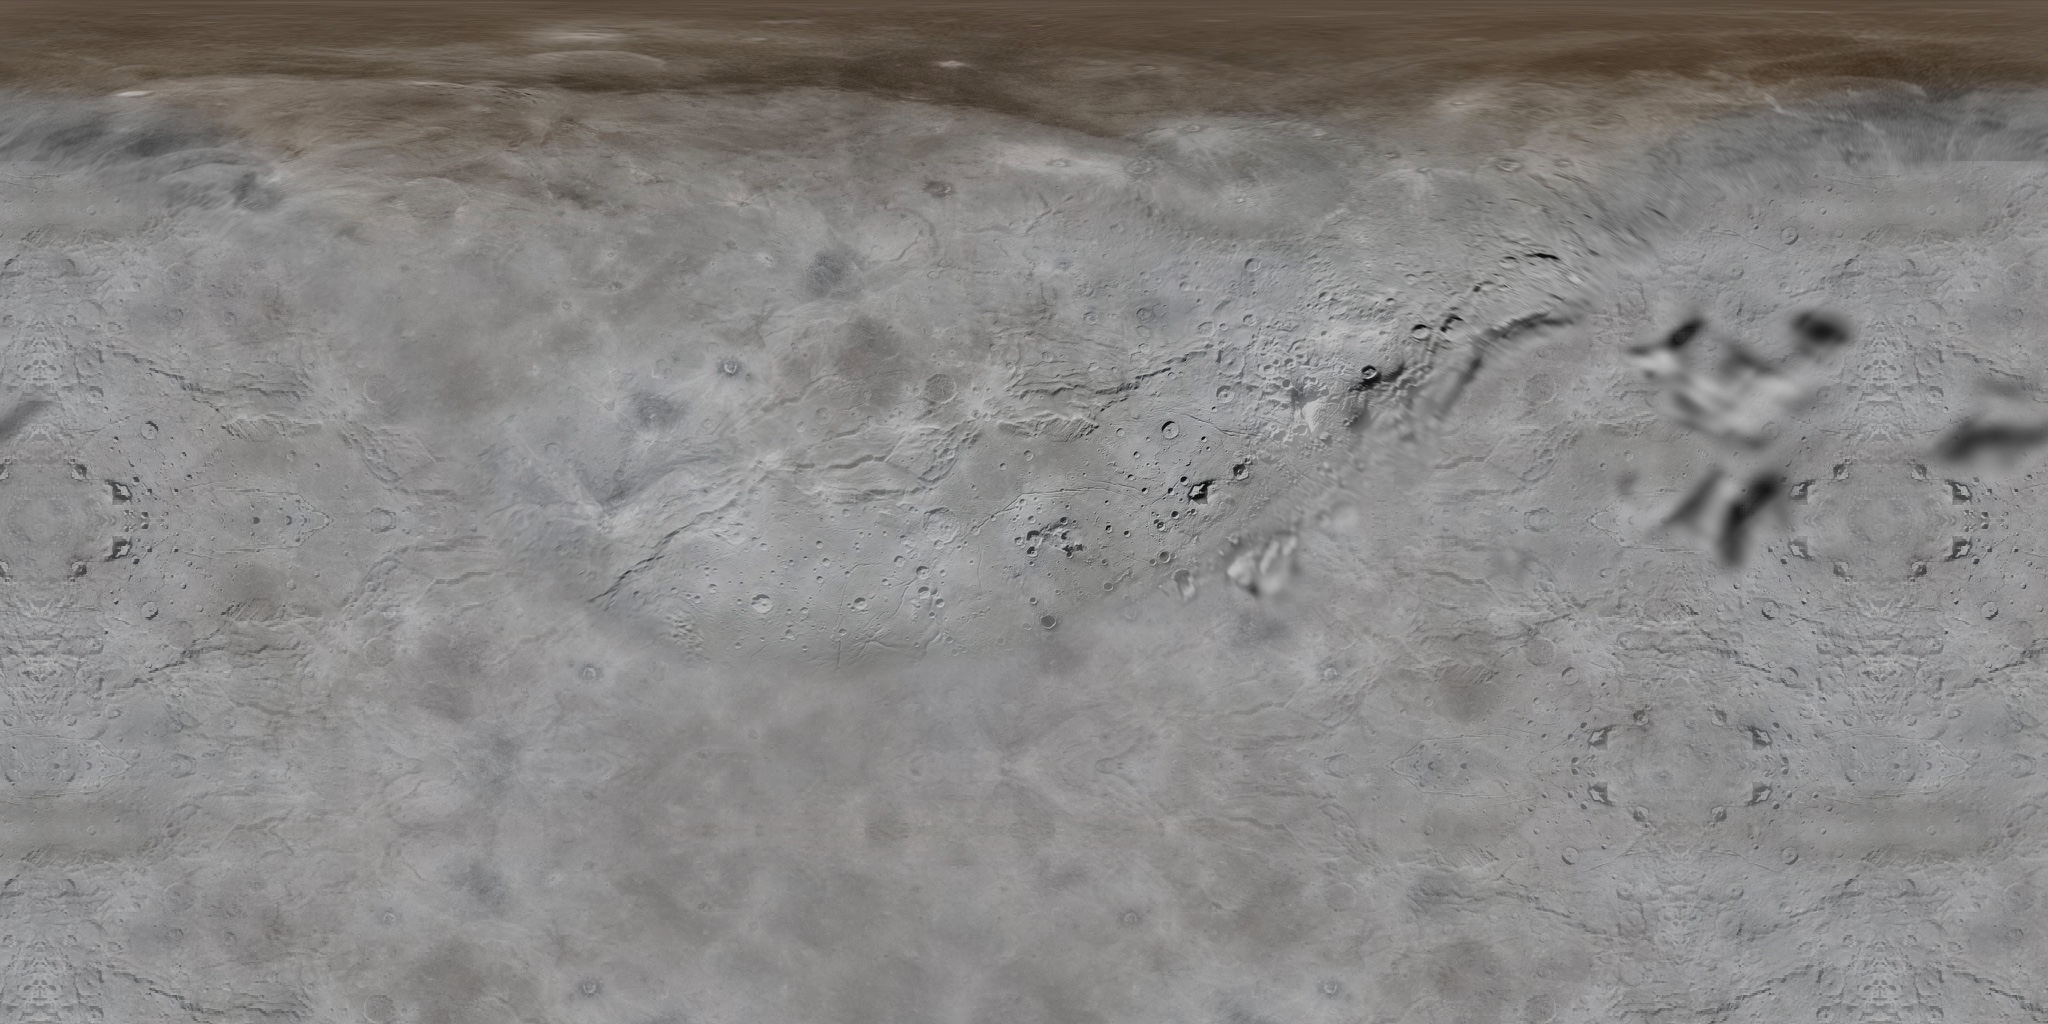
\includegraphics[width=\linewidth,height=4.4cm,keepaspectratio]{../public/textures/hd/charon_newhorizons.jpg}\\[2pt]
{\scriptsize\itshape\color{orbitarMuted} Planiglob desfășurat: Harta lunii Charon cu calota polară roșiatică Mordor Macula și canionul Serenity Chasma (NASA New Horizons, 2015).}
\end{tabular}
\end{center}


\begin{tcolorbox}[orbitardata, title={\textbf{Repere esențiale: Charon}}]
\small
\begin{itemize}[leftmargin=1.4em, itemsep=2pt, topsep=2pt]
  \item \textbf{Clasificare și orbită:} Satelit Natural (Lună) (orbitează în jurul: \textbf{Pluto}) \quad$\bullet$\quad \textbf{Distanță:} 39,480 UA ($\approx$ 5.906 milioane de kilometri)
  \item \textbf{Dimensiuni și masă:} rază medie 606 kilometri \quad$\bullet$\quad masă: 2,66e-4 $\times M_\oplus$
  \item \textbf{Gravitație și regim termic:} 0,029 $\times g_\oplus$ (0,28 m/s$^2$) \quad$\bullet$\quad temperatură medie: -220 $^\circ$C (înclinarea axei: Nespecificată)
  \item \textbf{Ciclu orbital și rotație:} perioadă orbitală (an): 6,387 zile pământești \quad$\bullet$\quad rotație (zi): 153,30 ore (6,39 zile pământești)
  \item \textbf{Durata călătoriei de pe Pământ:} cu viteza luminii ($1c$): \emph{5 ore și 30 de minute}; cu racheta ($50.000$ de kilometri pe oră): \emph{9 ani și jumătate (New Horizons)}; cu avionul ($900$ de kilometri pe oră): \emph{720 de ani}; cu mașina ($100$ de kilometri pe oră): \emph{6.500 de ani}.
  \item \textbf{Repere de scară și curiozitate:} Charon poartă la polul său nordic o \guillemotleft{}căciulă\guillemotright{} roșiatică de gheață colorată, iar pe la mijloc are un brâu de canioane uriașe! Dacă ai locui pe partea lui Pluto îndreptată spre Charon, ai vedea luna Charon stând nemișcată în exact același loc pe cer zi și noapte!
\end{itemize}
\end{tcolorbox}

\subsubsection*{Prezentare generală și profil astrofizic}
Descoperită în 1978 de James Christy, Charon are o rază de 606 kilometri (peste jumătate din diametrul lui Pluto). Centrul de masă comun (baricentrul) se află în spațiul liber dintre cele două corpuri, motiv pentru care sistemul Pluto--Charon este adesea numit o planetă pitică dublă. Charon este cel mai bun prieten al lui Pluto! Este atât de mare în comparație cu Pluto încât cei doi stau mereu față în față pe cer, ca doi dansatori care se țin de mâini. Charon poartă la polul său nordic o \guillemotleft{}căciulă\guillemotright{} roșiatică de gheață colorată, iar pe la mijloc are un brâu de canioane uriașe!

\subsubsection*{Alcătuirea fizică și structura internă}
Privind în profunzimea sa, alcătuirea fizică este organizată pe mai multe straturi și regiuni distincte, fiecare având un rol bine definit în evoluția și dinamica acestui obiect cosmic. În primul rând se remarcă \textbf{Interior de rocă (55\%) și gheață de apă (45\%)}, unde spre deosebire de Pluto, suprafața lui Charon este dominată de gheață de apă cristalină și hidrați de amoniac. În strânsă legătură cu această componentă se află \textbf{Serenity Chasma și centura de canioane}, un lanț de canioane lung de peste 1.000 de kilometri și adânc de 7--9 kilometri, format când un ocean subteran străvechi a înghețat și s-a extins. În completarea acestui ansamblu întâlnim \textbf{Calota polară Mordor Macula}, regiune polară roșiatică formată din metan scăpat din atmosfera lui Pluto, captat de polul rece al lui Charon și transformat în toline de razele UV.

\subsubsection*{Observații astronomice și istoricul explorării}
Fotografiată la rezoluție înaltă de sonda NASA New Horizons la 14 iulie 2015. Dacă ai locui pe partea lui Pluto îndreptată spre Charon, ai vedea luna Charon stând nemișcată în exact același loc pe cer zi și noapte!

\vspace{6pt}
\begin{tcolorbox}[orbitarquiz, title={\textbf{Întrebare de verificare \#34: Charon}}]
\textbf{De ce stau Pluto și Charon mereu cu aceeași față îndreptată unul spre celălalt?}
\begin{itemize}[leftmargin=2.2em, itemsep=2pt, topsep=4pt]
  \item[$\square$ \textbf{A.}] Ambele corpuri sunt în rotație sincronă reciprocă (blocare mareică dublă)
  \item[$\square$ \textbf{B.}] Pentru că sunt lipite între ele
  \item[$\square$ \textbf{C.}] Pentru că nu se rotesc deloc
  \item[$\square$ \textbf{D.}] Din cauza câmpului magnetic al lui Neptun
\end{itemize}
\vspace{2pt}
{\footnotesize\color{orbitarMuted}\textbf{Răspuns corect:} \textbf{A} (Ambele corpuri sunt în rotație sincronă reciprocă (blocare mareică dublă)). \emph{Pluto și Charon se rotesc în jurul axelor lor în exact 6,387 zile, având exact aceeași durată în care orbitează în jurul baricentrului lor comun.}}
\end{tcolorbox}
\clearpage


\subsection{Haumea}
\label{sec:body-haumea}
\vspace{-4pt}
{\large\itshape\color{orbitarAccent} Planeta pitică ovală cu inel propriu și rotație ultra-rapidă}\\[4pt]


\begin{center}
\begin{tabular}{@{}m{0.44\textwidth}@{\hspace{0.03\textwidth}}m{0.51\textwidth}@{}}
\centering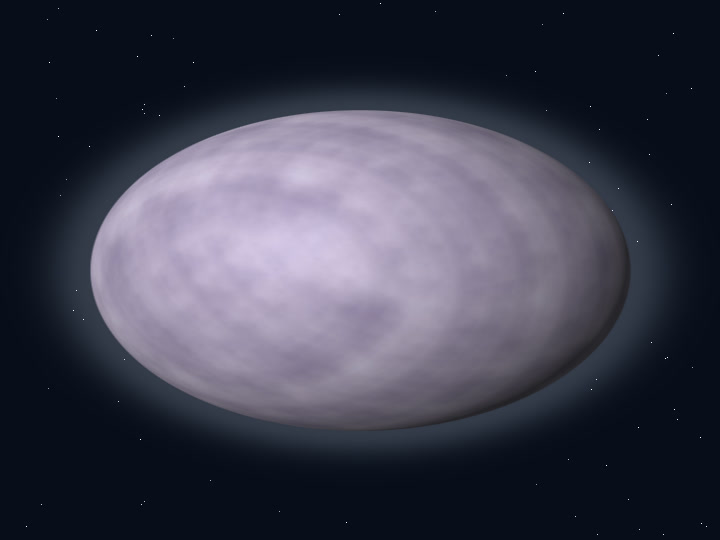
\includegraphics[width=\linewidth,height=4.4cm,keepaspectratio]{imagini/globuri/haumea.jpg}\\[2pt]
{\scriptsize\itshape\color{orbitarMuted} Vedere 3D a corpului ceresc (\textbf{Haumea})}
&
\centering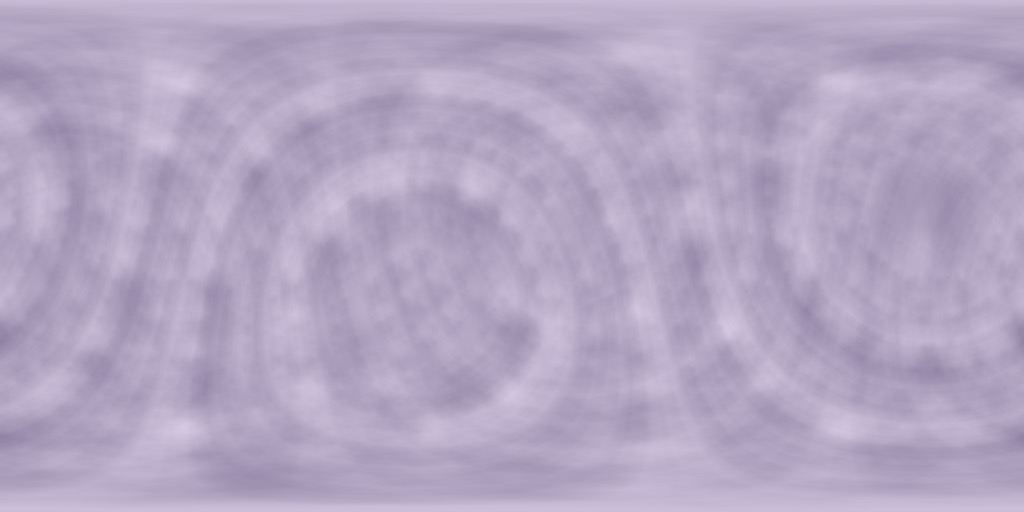
\includegraphics[width=\linewidth,height=4.4cm,keepaspectratio]{../public/textures/haumea.jpg}\\[2pt]
{\scriptsize\itshape\color{orbitarMuted} Planiglob desfășurat: Harta suprafeței de gheață cristalină și a petei roșiatice de pe planeta pitică elipsoidală Haumea.}
\end{tabular}
\end{center}


\begin{tcolorbox}[orbitardata, title={\textbf{Repere esențiale: Haumea}}]
\small
\begin{itemize}[leftmargin=1.4em, itemsep=2pt, topsep=2pt]
  \item \textbf{Clasificare și orbită:} Planetă Pitică \quad$\bullet$\quad \textbf{Distanță:} 43,130 UA ($\approx$ 6.452 milioane de kilometri)
  \item \textbf{Dimensiuni și masă:} rază medie 780 de kilometri \quad$\bullet$\quad masă: 6,70e-4 $\times M_\oplus$
  \item \textbf{Gravitație și regim termic:} 0,041 $\times g_\oplus$ (0,40 m/s$^2$) \quad$\bullet$\quad temperatură medie: -241 $^\circ$C (înclinarea axei: Nespecificată)
  \item \textbf{Ciclu orbital și rotație:} perioadă orbitală (an): 103.774 zile ($\approx$ 284,12 ani pământești) \quad$\bullet$\quad rotație (zi): 3,92 ore (0,16 zile pământești) (elemente kepleriene: $a = 43,130$ UA, $e = 0,1950$, $i = 28,19^\circ$, $\Omega = 122,1^\circ$, $\omega = 239,0^\circ$)
  \item \textbf{Durata călătoriei de pe Pământ:} cu viteza luminii ($1c$): \emph{6 ore}; cu racheta ($50.000$ de kilometri pe oră): \emph{14 ani}; cu avionul ($900$ de kilometri pe oră): \emph{790 de ani}; cu mașina ($100$ de kilometri pe oră): \emph{7.100 de ani}.
  \item \textbf{Repere de scară și curiozitate:} Haumea are forma unei pietre plate de râu sau a unui ou alb de Paște care se învârte amețitor! Haumea are două luni mici (Hi'iaka și Namaka) și chiar și un inel subțire în jurul ei, ca un mini-Saturn!
\end{itemize}
\end{tcolorbox}

\subsubsection*{Prezentare generală și profil astrofizic}
Situată în Centura Kuiper la aproximativ 43 UA, Haumea are forma unui elipsoid triaxial (aproximativ 2.100 $\times$ 1.680 $\times$ 1.070 de kilometri) din cauza perioadei de rotație de doar 3,9 ore. În 2017, printr-o ocultație stelară, s-a descoperit că posedă un sistem de inele. Haumea este cel mai rapid titirez mare din Sistemul Solar! O zi pe Haumea durează mai puțin de 4 ore, iar din această cauză s-a alungit ca o minge de rugby! Haumea are forma unei pietre plate de râu sau a unui ou alb de Paște care se învârte amețitor!

\subsubsection*{Alcătuirea fizică și structura internă}
Privind în profunzimea sa, alcătuirea fizică este organizată pe mai multe straturi și regiuni distincte, fiecare având un rol bine definit în evoluția și dinamica acestui obiect cosmic. În primul rând se remarcă \textbf{Interior stâncos diferențiat}, densitate ridicată (aproximativ 2,0 g/cm$^3$) rezultată după un impact antic care i-a accelerat rotația. În strânsă legătură cu această componentă se află \textbf{Crustă subțire de gheață cristalină pură}, unde spre deosebire de alte obiecte transneptuniene, suprafața ei este acoperită cu gheață de apă cristalină. În completarea acestui ansamblu întâlnim \textbf{Inel ecuatorial (rază aproximativ 2.287 de kilometri)}, primul inel descoperit în jurul unui obiect transneptunian.

\subsubsection*{Observații astronomice și istoricul explorării}
Descoperită în 2004 și caracterizată prin ocultații stelare și observații ale telescoapelor spațiale. Haumea are două luni mici (Hi'iaka și Namaka) și chiar și un inel subțire în jurul ei, ca un mini-Saturn!

\vspace{6pt}
\begin{tcolorbox}[orbitarquiz, title={\textbf{Întrebare de verificare \#35: Haumea}}]
\textbf{De ce are planeta pitică Haumea o formă alungită, asemănătoare unei mingi de rugby?}
\begin{itemize}[leftmargin=2.2em, itemsep=2pt, topsep=4pt]
  \item[$\square$ \textbf{A.}] Din cauza căldurii Soarelui
  \item[$\square$ \textbf{B.}] Din cauza rotației extrem de rapide (o rotație completă în mai puțin de 4 ore)
  \item[$\square$ \textbf{C.}] Pentru că este atrasă de Marte
  \item[$\square$ \textbf{D.}] Pentru că este făcută din gaz
\end{itemize}
\vspace{2pt}
{\footnotesize\color{orbitarMuted}\textbf{Răspuns corect:} \textbf{B} (Din cauza rotației extrem de rapide (o rotație completă în mai puțin de 4 ore)). \emph{Forța centrifugă produsă de rotația în doar 3,9 ore i-a deformat corpul într-un elipsoid alungit.}}
\end{tcolorbox}
\clearpage


\subsection{Makemake}
\label{sec:body-makemake}
\vspace{-4pt}
{\large\itshape\color{orbitarAccent} Lumea roșiatică de metan înghețat din Centura Kuiper}\\[4pt]


\begin{center}
\begin{tabular}{@{}m{0.44\textwidth}@{\hspace{0.03\textwidth}}m{0.51\textwidth}@{}}
\centering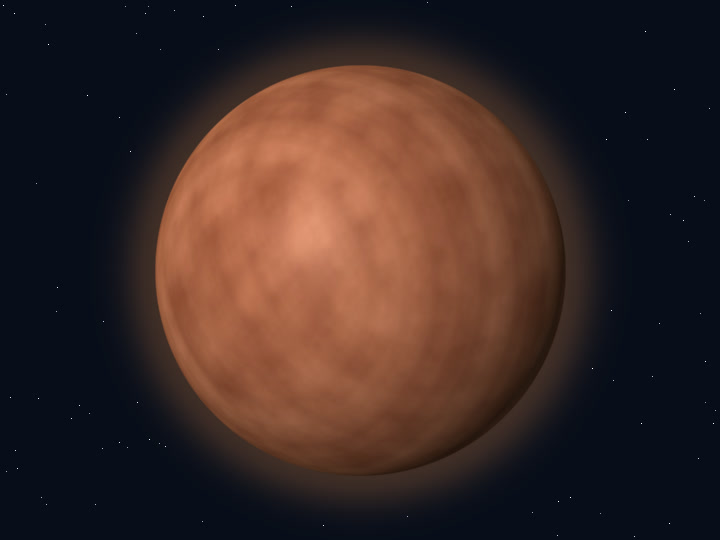
\includegraphics[width=\linewidth,height=4.4cm,keepaspectratio]{imagini/globuri/makemake.jpg}\\[2pt]
{\scriptsize\itshape\color{orbitarMuted} Vedere 3D a corpului ceresc (\textbf{Makemake})}
&
\centering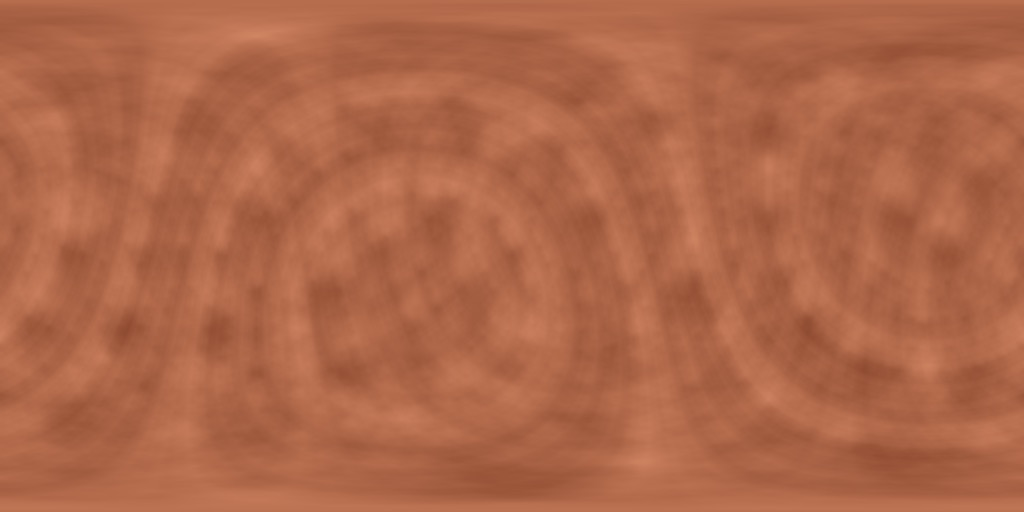
\includegraphics[width=\linewidth,height=4.4cm,keepaspectratio]{../public/textures/makemake.jpg}\\[2pt]
{\scriptsize\itshape\color{orbitarMuted} Planiglob desfășurat: Harta suprafeței bogate în toline roșiatice și metan înghețat a planetei pitice Makemake din Centura Kuiper.}
\end{tabular}
\end{center}


\begin{tcolorbox}[orbitardata, title={\textbf{Repere esențiale: Makemake}}]
\small
\begin{itemize}[leftmargin=1.4em, itemsep=2pt, topsep=2pt]
  \item \textbf{Clasificare și orbită:} Planetă Pitică \quad$\bullet$\quad \textbf{Distanță:} 45,430 UA ($\approx$ 6.796 milioane de kilometri)
  \item \textbf{Dimensiuni și masă:} rază medie 715 kilometri \quad$\bullet$\quad masă: 5,00e-4 $\times M_\oplus$
  \item \textbf{Gravitație și regim termic:} 0,050 $\times g_\oplus$ (0,49 m/s$^2$) \quad$\bullet$\quad temperatură medie: -243 $^\circ$C (înclinarea axei: Nespecificată)
  \item \textbf{Ciclu orbital și rotație:} perioadă orbitală (an): 111.845 zile ($\approx$ 306,21 ani pământești) \quad$\bullet$\quad rotație (zi): 22,83 ore (0,95 zile pământești) (elemente kepleriene: $a = 45,430$ UA, $e = 0,1610$, $i = 28,98^\circ$, $\Omega = 79,6^\circ$, $\omega = 294,8^\circ$)
  \item \textbf{Durata călătoriei de pe Pământ:} cu viteza luminii ($1c$): \emph{6 ore și 18 minute}; cu racheta ($50.000$ de kilometri pe oră): \emph{15 ani}; cu avionul ($900$ de kilometri pe oră): \emph{830 de ani}; cu mașina ($100$ de kilometri pe oră): \emph{7.500 de ani}.
  \item \textbf{Repere de scară și curiozitate:} Makemake este ca un bulgăre mare de înghețată de căpșuni la marginea Sistemului Solar! A fost descoperită chiar în zilele de după Paște în anul 2005, așa că porecla ei inițială a fost \guillemotleft{}Iepurașul de Paște\guillemotright{} (Easterbunny)!
\end{itemize}
\end{tcolorbox}

\subsubsection*{Prezentare generală și profil astrofizic}
A doua planetă pitică ca strălucire din Centura Kuiper (după Pluto), Makemake orbitează la o distanță medie de 45,4 UA în 306 ani terestri. Are o suprafață bogată în pelete de metan și etan înghețat și un mic satelit întunecat botezat MK 2. Makemake este unul dintre cele mai strălucitoare obiecte din Centura Kuiper, numit după zeul primăverii și al fertilității din Insula Paștelui! Makemake este ca un bulgăre mare de înghețată de căpșuni la marginea Sistemului Solar!

\subsubsection*{Alcătuirea fizică și structura internă}
Privind în profunzimea sa, alcătuirea fizică este organizată pe mai multe straturi și regiuni distincte, fiecare având un rol bine definit în evoluția și dinamica acestui obiect cosmic. În primul rând se remarcă \textbf{Nucleu de silicați și gheață}, interior rece compus dintr-un amestec de rocă și gheață de apă. În strânsă legătură cu această componentă se află \textbf{Suprafață acoperită cu metan, etan și toline}, unde radiația UV solară transformă metanul în compuși organici roșiatici (toline). În completarea acestui ansamblu întâlnim \textbf{Exosferă sezonieră infimă}, unde ocultațiile stelare arată că Makemake nu posedă o atmosferă globală substanțială.

\subsubsection*{Observații astronomice și istoricul explorării}
Descoperită în martie 2005 la Observatorul Palomar; satelitul său MK 2 a fost descoperit cu Telescopul Hubble în 2016. A fost descoperită chiar în zilele de după Paște în anul 2005, așa că porecla ei inițială a fost \guillemotleft{}Iepurașul de Paște\guillemotright{} (Easterbunny)!

\vspace{6pt}
\begin{tcolorbox}[orbitarquiz, title={\textbf{Întrebare de verificare \#36: Makemake}}]
\textbf{Care a fost porecla dată de astronomi planetei pitice Makemake la descoperire?}
\begin{itemize}[leftmargin=2.2em, itemsep=2pt, topsep=4pt]
  \item[$\square$ \textbf{A.}] Moș Crăciun
  \item[$\square$ \textbf{B.}] Iepurașul de Paște (Easterbunny)
  \item[$\square$ \textbf{C.}] Micul Prinț
  \item[$\square$ \textbf{D.}] Steaua Polară
\end{itemize}
\vspace{2pt}
{\footnotesize\color{orbitarMuted}\textbf{Răspuns corect:} \textbf{B} (Iepurașul de Paște (Easterbunny)). \emph{Fiind descoperită la scurt timp după Paștele anului 2005, echipa a poreclit-o \guillemotleft{}Easterbunny\guillemotright{}, iar numele oficial Makemake provine din mitologia Rapa Nui (Insula Paștelui).}}
\end{tcolorbox}
\clearpage


\subsection{Eris}
\label{sec:body-eris}
\vspace{-4pt}
{\large\itshape\color{orbitarAccent} Cea mai masivă planetă pitică cunoscută, din Discul Împrăștiat}\\[4pt]


\begin{center}
\begin{tabular}{@{}m{0.44\textwidth}@{\hspace{0.03\textwidth}}m{0.51\textwidth}@{}}
\centering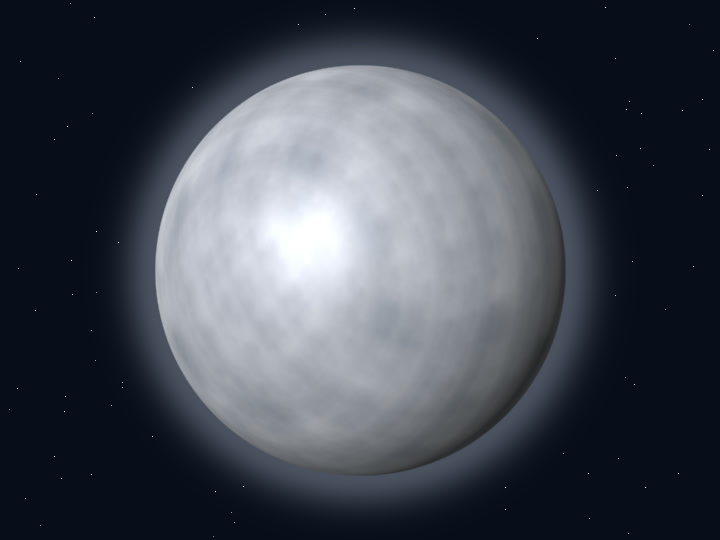
\includegraphics[width=\linewidth,height=4.4cm,keepaspectratio]{imagini/globuri/eris.jpg}\\[2pt]
{\scriptsize\itshape\color{orbitarMuted} Vedere 3D a corpului ceresc (\textbf{Eris})}
&
\centering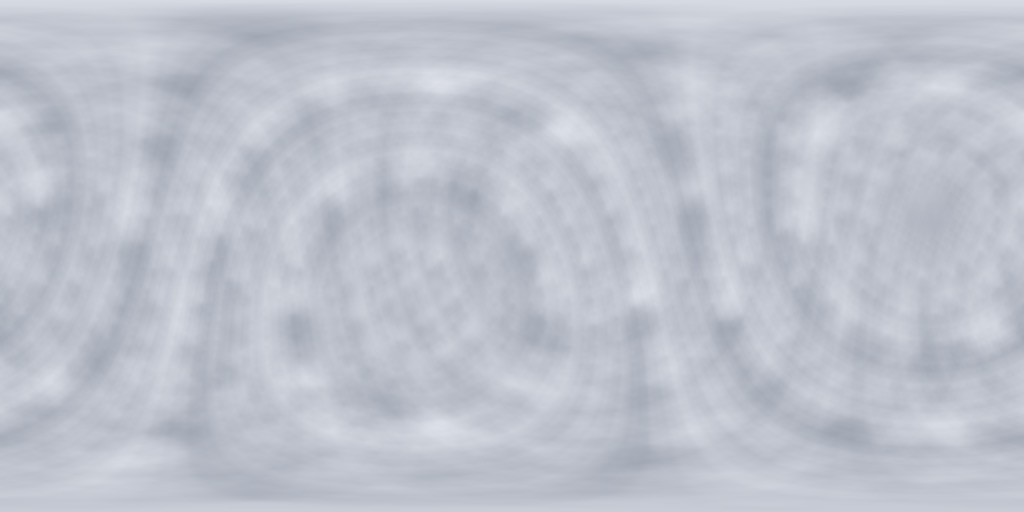
\includegraphics[width=\linewidth,height=4.4cm,keepaspectratio]{../public/textures/eris.jpg}\\[2pt]
{\scriptsize\itshape\color{orbitarMuted} Planiglob desfășurat: Harta artistică științifică a suprafeței înghețate și extrem de reflectante de metan a planetei pitice Eris.}
\end{tabular}
\end{center}


\begin{tcolorbox}[orbitardata, title={\textbf{Repere esențiale: Eris}}]
\small
\begin{itemize}[leftmargin=1.4em, itemsep=2pt, topsep=2pt]
  \item \textbf{Clasificare și orbită:} Planetă Pitică \quad$\bullet$\quad \textbf{Distanță:} 67,860 UA ($\approx$ 10.152 milioane de kilometri)
  \item \textbf{Dimensiuni și masă:} rază medie 1.163 de kilometri \quad$\bullet$\quad masă: 0,003 $\times M_\oplus$
  \item \textbf{Gravitație și regim termic:} 0,084 $\times g_\oplus$ (0,82 m/s$^2$) \quad$\bullet$\quad temperatură medie: -243 $^\circ$C (înclinarea axei: Nespecificată)
  \item \textbf{Ciclu orbital și rotație:} perioadă orbitală (an): 203.830 zile ($\approx$ 558,06 ani pământești) \quad$\bullet$\quad rotație (zi): 25,90 ore (1,08 zile pământești) (elemente kepleriene: $a = 67,860$ UA, $e = 0,4360$, $i = 44,04^\circ$, $\Omega = 35,9^\circ$, $\omega = 151,6^\circ$)
  \item \textbf{Durata călătoriei de pe Pământ:} cu viteza luminii ($1c$): \emph{9 ore și 25 de minute}; cu racheta ($50.000$ de kilometri pe oră): \emph{25 de ani}; cu avionul ($900$ de kilometri pe oră): \emph{1.200 de ani}; cu mașina ($100$ de kilometri pe oră): \emph{11.000 de ani}.
  \item \textbf{Repere de scară și curiozitate:} Eris este aproape geamănă ca mărime cu Pluto, dar cântărește puțin mai mult pentru că are mai multă piatră în interior! Pe Eris este atât de frig încât toată atmosfera ei a înghețat și s-a așternut pe sol ca o pătură sclipitoare de promoroacă!
\end{itemize}
\end{tcolorbox}

\subsubsection*{Prezentare generală și profil astrofizic}
Descoperită în 2005 de echipa lui Mike Brown la Observatorul Palomar, Eris este cu 27\% mai masivă decât Pluto. Orbita sa puternic înclinată (44$^\circ$) o poartă până la 97 UA de Soare în Discul Împrăștiat, iar un an pe Eris durează 558 de ani terestri. Eris este o lume albă ca zăpada, aflată de peste două ori mai departe de Soare decât Neptun! Descoperirea ei i-a făcut pe astronomi să inventeze categoria de \guillemotleft{}planetă pitică\guillemotright{}. Eris este aproape geamănă ca mărime cu Pluto, dar cântărește puțin mai mult pentru că are mai multă piatră în interior!

\subsubsection*{Alcătuirea fizică și structura internă}
Privind în profunzimea sa, alcătuirea fizică este organizată pe mai multe straturi și regiuni distincte, fiecare având un rol bine definit în evoluția și dinamica acestui obiect cosmic. În primul rând se remarcă \textbf{Nucleu dens de silicați}, care constituie aproximativ 85\% din masa corpului (densitate medie 2,52 g/cm$^3$). În strânsă legătură cu această componentă se află \textbf{Manta de gheață de apă}, înveliș glaciar rigid la temperaturi apropiate de zero absolut. În completarea acestui ansamblu întâlnim \textbf{Suprafață ultra-reflectivă de metan și azot înghețat}, care reflectă 96\% din lumina solară incidentă.

\subsubsection*{Observații astronomice și istoricul explorării}
Studiată prin telescoapele Hubble, Keck și James Webb, împreună cu satelitul său Dysnomia. Pe Eris este atât de frig încât toată atmosfera ei a înghețat și s-a așternut pe sol ca o pătură sclipitoare de promoroacă!

\vspace{6pt}
\begin{tcolorbox}[orbitarquiz, title={\textbf{Întrebare de verificare \#37: Eris}}]
\textbf{Ce eveniment astronomic a determinat descoperirea planetei pitice Eris în 2005?}
\begin{itemize}[leftmargin=2.2em, itemsep=2pt, topsep=4pt]
  \item[$\square$ \textbf{A.}] Lansarea telescopului Hubble
  \item[$\square$ \textbf{B.}] Definirea oficială a categoriei de \guillemotleft{}planetă pitică\guillemotright{} și reclasificarea lui Pluto în 2006
  \item[$\square$ \textbf{C.}] Asolizarea pe Marte
  \item[$\square$ \textbf{D.}] Descoperirea inelelor lui Saturn
\end{itemize}
\vspace{2pt}
{\footnotesize\color{orbitarMuted}\textbf{Răspuns corect:} \textbf{B} (Definirea oficială a categoriei de \guillemotleft{}planetă pitică\guillemotright{} și reclasificarea lui Pluto în 2006). \emph{Deoarece Eris s-a dovedit mai masivă decât Pluto, Uniunea Astronomică Internațională a stabilit în 2006 criteriile pentru planete și planete pitice.}}
\end{tcolorbox}
\clearpage


\section{Asteroizi Principali și Obiecte din Apropierea Pământului}

\subsection{4 Vesta}
\label{sec:body-vesta}
\vspace{-4pt}
{\large\itshape\color{orbitarAccent} Cel mai strălucitor asteroid și protoplanetă stâncoasă}\\[4pt]


\begin{center}
\begin{tabular}{@{}m{0.44\textwidth}@{\hspace{0.03\textwidth}}m{0.51\textwidth}@{}}
\centering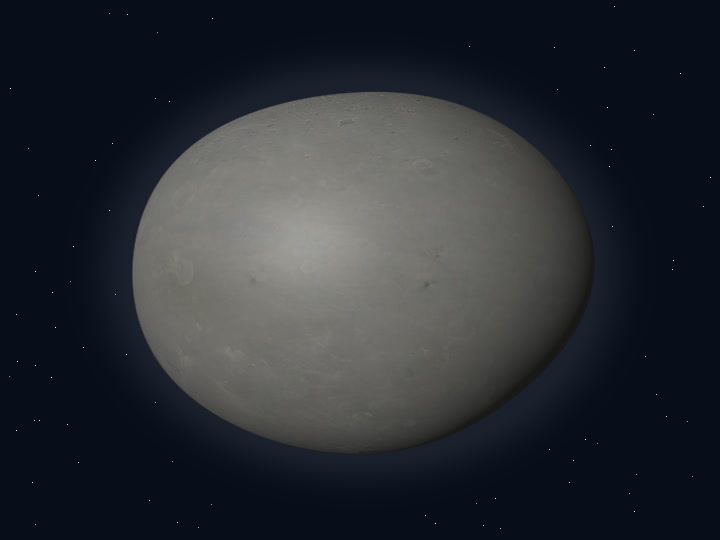
\includegraphics[width=\linewidth,height=4.4cm,keepaspectratio]{imagini/globuri/vesta.jpg}\\[2pt]
{\scriptsize\itshape\color{orbitarMuted} Vedere 3D a corpului ceresc (\textbf{4 Vesta})}
&
\centering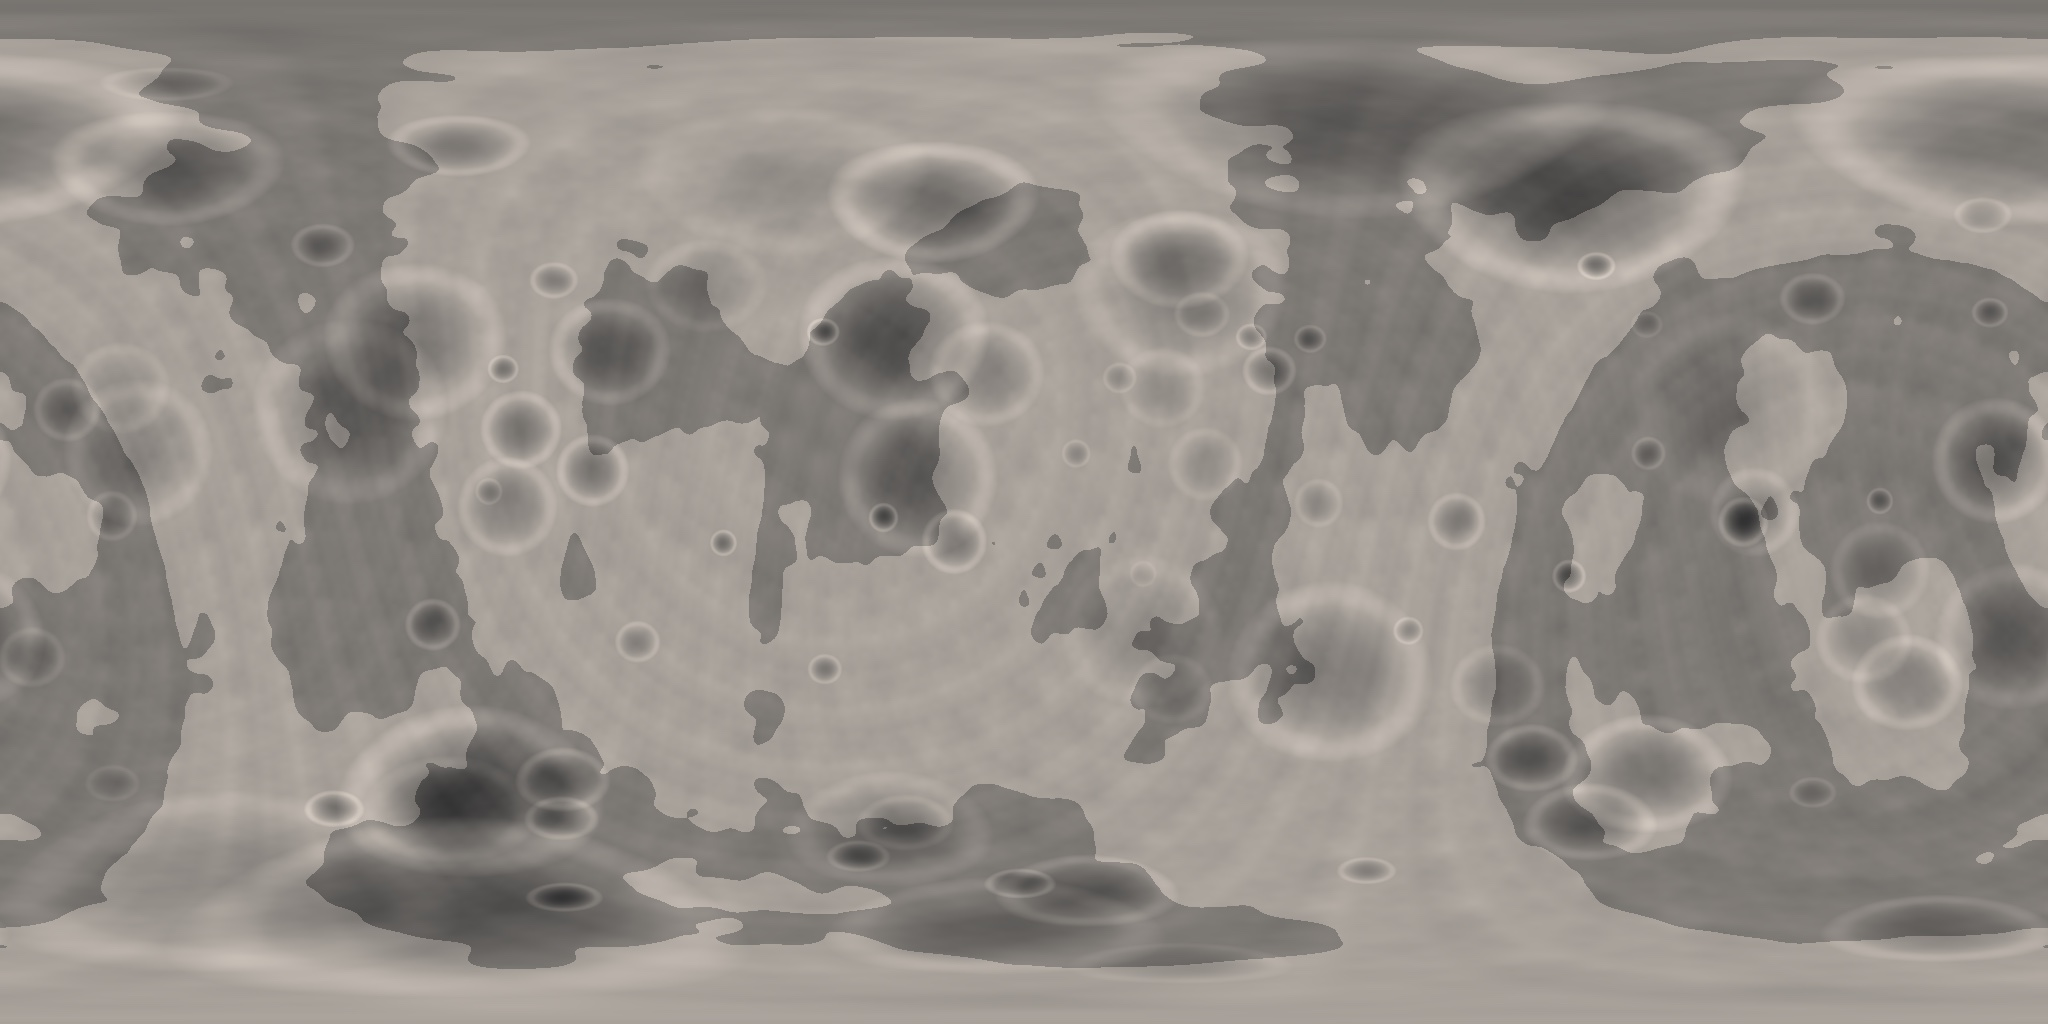
\includegraphics[width=\linewidth,height=4.4cm,keepaspectratio]{../public/textures/hd/vesta_dawn.jpg}\\[2pt]
{\scriptsize\itshape\color{orbitarMuted} Planiglob desfășurat: Harta topografică a protoplanetei 4 Vesta, obținută de sonda NASA Dawn în 2011--2012.}
\end{tabular}
\end{center}


\begin{tcolorbox}[orbitardata, title={\textbf{Repere esențiale: 4 Vesta}}]
\small
\begin{itemize}[leftmargin=1.4em, itemsep=2pt, topsep=2pt]
  \item \textbf{Clasificare și orbită:} Asteroid \quad$\bullet$\quad \textbf{Distanță:} 2,362 UA ($\approx$ 353 milioane de kilometri)
  \item \textbf{Dimensiuni și masă:} rază medie 262,7 de kilometri \quad$\bullet$\quad masă: 4,30e-5 $\times M_\oplus$
  \item \textbf{Gravitație și regim termic:} 0,025 $\times g_\oplus$ (0,25 m/s$^2$) \quad$\bullet$\quad temperatură medie: -60 $^\circ$C (înclinarea axei: Nespecificată)
  \item \textbf{Ciclu orbital și rotație:} perioadă orbitală (an): 1.325,75 zile ($\approx$ 3,63 ani pământești) \quad$\bullet$\quad rotație (zi): 5,34 ore (0,22 zile pământești) (elemente kepleriene: $a = 2,362$ UA, $e = 0,0890$, $i = 7,14^\circ$, $\Omega = 103,8^\circ$, $\omega = 151,2^\circ$)
  \item \textbf{Durata călătoriei de pe Pământ:} cu viteza luminii ($1c$): \emph{19 minute}; cu racheta ($50.000$ de kilometri pe oră): \emph{1,2 ani}; cu avionul ($900$ de kilometri pe oră): \emph{25 de ani}; cu mașina ($100$ de kilometri pe oră): \emph{230 de ani}.
  \item \textbf{Repere de scară și curiozitate:} Vesta este ca un cartof uriaș din stâncă, cu un munte la polul sud aproape la fel de înalt ca cel de pe Marte! Bucăți rupte din Vesta acum milioane de ani au căzut pe Pământ sub formă de meteoriți pe care îi putem vedea în muzee!
\end{itemize}
\end{tcolorbox}

\subsubsection*{Prezentare generală și profil astrofizic}
Descoperită în 1807 de Heinrich Olbers, 4 Vesta este o protoplanetă diferențiată (cu nucleu metalic, manta și scoarță bazaltică). Bazinul de impact Rheasilvia de la polul sud are 500 de kilometri diametru și un vârf central de 22 de kilometri înălțime. Vesta este un asteroid uriaș din piatră, atât de luminos încât uneori poate fi văzut de pe Pământ chiar și fără telescop, într-o noapte foarte senină! Vesta este ca un cartof uriaș din stâncă, cu un munte la polul sud aproape la fel de înalt ca cel de pe Marte!

\subsubsection*{Alcătuirea fizică și structura internă}
Privind în profunzimea sa, alcătuirea fizică este organizată pe mai multe straturi și regiuni distincte, fiecare având un rol bine definit în evoluția și dinamica acestui obiect cosmic. În primul rând se remarcă \textbf{Nucleu de fier-nichel (rază aproximativ 110 kilometri)}, dovadă că Vesta s-a topit și s-a diferențiat ca o planetă telurică în primele milioane de ani. În strânsă legătură cu această componentă se află \textbf{Manta de olivină}, expusă la suprafață în uriașul bazin de impact Rheasilvia. În completarea acestui ansamblu întâlnim \textbf{Scoarță bazaltică (sursa meteoriților HED)}, sursă pentru meteoriții de tip howardit-eucrit-diogenit găsiți pe Pământ.

\subsubsection*{Observații astronomice și istoricul explorării}
Orbitată și cartografiată în detaliu de sonda NASA Dawn între iulie 2011 și septembrie 2012. Bucăți rupte din Vesta acum milioane de ani au căzut pe Pământ sub formă de meteoriți pe care îi putem vedea în muzee!

\vspace{6pt}
\begin{tcolorbox}[orbitarquiz, title={\textbf{Întrebare de verificare \#38: 4 Vesta}}]
\textbf{Ce au descoperit oamenii de știință în centrul bazinului Rheasilvia de pe asteroidul Vesta?}
\begin{itemize}[leftmargin=2.2em, itemsep=2pt, topsep=4pt]
  \item[$\square$ \textbf{A.}] Un lac de apă
  \item[$\square$ \textbf{B.}] Un munte central înalt de 22 de kilometri, aproape cât Olympus Mons de pe Marte
  \item[$\square$ \textbf{C.}] Un vulcan activ
  \item[$\square$ \textbf{D.}] O sondă extraterestră
\end{itemize}
\vspace{2pt}
{\footnotesize\color{orbitarMuted}\textbf{Răspuns corect:} \textbf{B} (Un munte central înalt de 22 de kilometri, aproape cât Olympus Mons de pe Marte). \emph{Impactul colosal care a creat craterul Rheasilvia a ridicat în centru un munte de 22 de kilometri înălțime, unul dintre cele mai înalte vârfuri din Sistemul Solar.}}
\end{tcolorbox}
\clearpage


\subsection{2 Pallas}
\label{sec:body-pallas}
\vspace{-4pt}
{\large\itshape\color{orbitarAccent} Al doilea asteroid descoperit, cu o orbită puternic înclinată}\\[4pt]


\begin{center}
\begin{tabular}{@{}m{0.44\textwidth}@{\hspace{0.03\textwidth}}m{0.51\textwidth}@{}}
\centering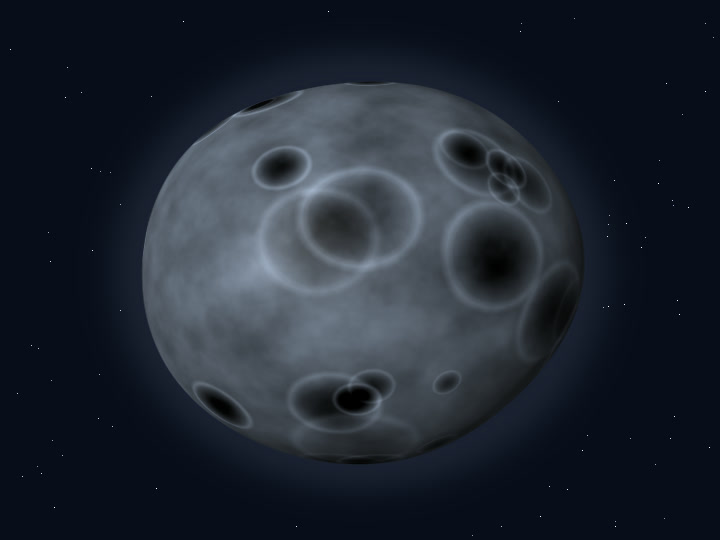
\includegraphics[width=\linewidth,height=4.4cm,keepaspectratio]{imagini/globuri/pallas.jpg}\\[2pt]
{\scriptsize\itshape\color{orbitarMuted} Vedere 3D a corpului ceresc (\textbf{2 Pallas})}
&
\centering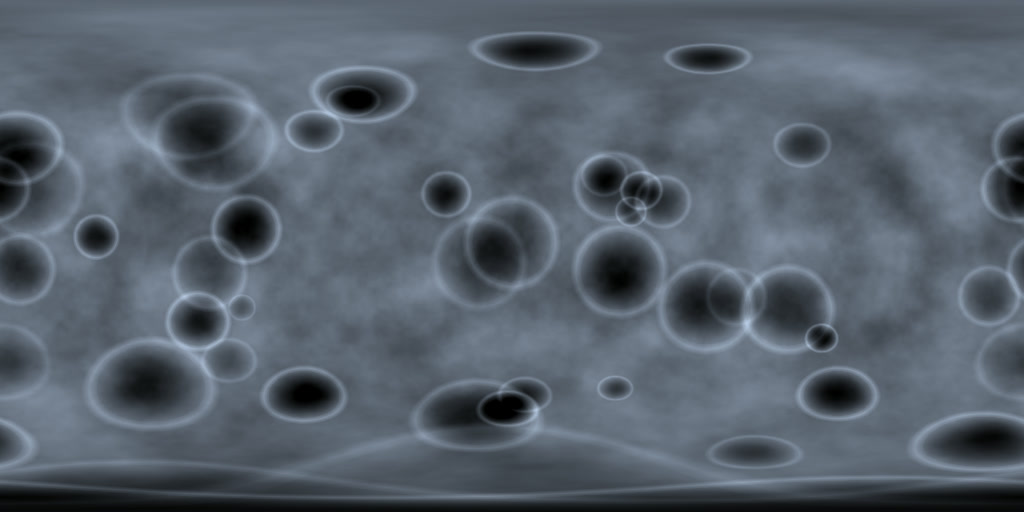
\includegraphics[width=\linewidth,height=4.4cm,keepaspectratio]{imagini/globuri/pallas_map.jpg}\\[2pt]
{\scriptsize\itshape\color{orbitarMuted} Planiglob desfășurat: Harta desfășurată a reliefului craterizat al asteroidului 2 Pallas din Centura Principală.}
\end{tabular}
\end{center}


\begin{tcolorbox}[orbitardata, title={\textbf{Repere esențiale: 2 Pallas}}]
\small
\begin{itemize}[leftmargin=1.4em, itemsep=2pt, topsep=2pt]
  \item \textbf{Clasificare și orbită:} Asteroid \quad$\bullet$\quad \textbf{Distanță:} 2,773 UA ($\approx$ 415 milioane de kilometri)
  \item \textbf{Dimensiuni și masă:} rază medie 256 de kilometri \quad$\bullet$\quad masă: 3,40e-5 $\times M_\oplus$
  \item \textbf{Gravitație și regim termic:} 0,022 $\times g_\oplus$ (0,22 m/s$^2$) \quad$\bullet$\quad temperatură medie: -109 $^\circ$C (înclinarea axei: Nespecificată)
  \item \textbf{Ciclu orbital și rotație:} perioadă orbitală (an): 1.685,9 zile ($\approx$ 4,62 ani pământești) \quad$\bullet$\quad rotație (zi): 7,81 ore (0,33 zile pământești) (elemente kepleriene: $a = 2,773$ UA, $e = 0,2310$, $i = 34,84^\circ$, $\Omega = 173,0^\circ$, $\omega = 310,0^\circ$)
  \item \textbf{Durata călătoriei de pe Pământ:} cu viteza luminii ($1c$): \emph{23 de minute}; cu racheta ($50.000$ de kilometri pe oră): \emph{2 ani}; cu avionul ($900$ de kilometri pe oră): \emph{33 de ani}; cu mașina ($100$ de kilometri pe oră): \emph{300 de ani}.
  \item \textbf{Repere de scară și curiozitate:} În timp ce majoritatea asteroizilor merg pe aceeași \guillemotleft{}autostradă\guillemotright{} în jurul Soarelui, Pallas zboară pe o pistă înclinată ca un montagne-russe! A fost al doilea asteroid descoperit vreodată, în anul 1802, la doar un an după Ceres!
\end{itemize}
\end{tcolorbox}

\subsubsection*{Prezentare generală și profil astrofizic}
Cu un diametru mediu de 512 kilometri, 2 Pallas conține aproximativ 7\% din masa Centurii de Asteroizi. Înclinarea orbitală neobișnuit de mare (34,8$^\circ$) provoacă coliziuni la viteze medii mult mai ridicate decât la alți asteroizi, dându-i o morfologie intens craterizată. Pallas este unul dintre cei mai mari asteroizi din Sistemul Solar și are o suprafață atât de plină de cratere încât seamănă cu o minge de golf! În timp ce majoritatea asteroizilor merg pe aceeași \guillemotleft{}autostradă\guillemotright{} în jurul Soarelui, Pallas zboară pe o pistă înclinată ca un montagne-russe!

\subsubsection*{Alcătuirea fizică și structura internă}
Privind în profunzimea sa, alcătuirea fizică este organizată pe mai multe straturi și regiuni distincte, fiecare având un rol bine definit în evoluția și dinamica acestui obiect cosmic. În primul rând se remarcă \textbf{Interior bogat în silicați hidratați}, compoziție asemănătoare condritelor carbonice sărace în apă. În strânsă legătură cu această componentă se află \textbf{Suprafață saturată de cratere (\guillemotleft{}golf-ball\guillemotright{})}, observată cu rezoluție înaltă prin instrumentul SPHERE al Very Large Telescope (ESO). În completarea acestui ansamblu întâlnim \textbf{Depozite luminoase de sare}, vizibile în unele cratere, indicând o evoluție termică timpurie.

\subsubsection*{Observații astronomice și istoricul explorării}
Descoperită în 1802 de Heinrich Olbers; din cauza înclinării orbitale mari (34,8$^\circ$), nicio sondă nu a putut încă să intre pe orbita sa. A fost al doilea asteroid descoperit vreodată, în anul 1802, la doar un an după Ceres!

\vspace{6pt}
\begin{tcolorbox}[orbitarquiz, title={\textbf{Întrebare de verificare \#39: 2 Pallas}}]
\textbf{De ce seamănă suprafața asteroidului Pallas cu o minge de golf?}
\begin{itemize}[leftmargin=2.2em, itemsep=2pt, topsep=4pt]
  \item[$\square$ \textbf{A.}] A fost sculptată de vânt
  \item[$\square$ \textbf{B.}] Orbita sa foarte înclinată (34,8$^\circ$) produce ciocniri extrem de violente și numeroase cu alți asteroizi
  \item[$\square$ \textbf{C.}] Este acoperită cu gheață moale
  \item[$\square$ \textbf{D.}] Are vulcani mici
\end{itemize}
\vspace{2pt}
{\footnotesize\color{orbitarMuted}\textbf{Răspuns corect:} \textbf{B} (Orbita sa foarte înclinată (34,8$^\circ$) produce ciocniri extrem de violente și numeroase cu alți asteroizi). \emph{Traversând centura de asteroizi sub un unghi mare, Pallas suferă impacturi la viteze de până la patru ori mai mari decât media din centură.}}
\end{tcolorbox}
\clearpage


\subsection{16 Psyche}
\label{sec:body-psyche}
\vspace{-4pt}
{\large\itshape\color{orbitarAccent} Lumea metalică unică din Centura de Asteroizi}\\[4pt]


\begin{center}
\begin{tabular}{@{}m{0.44\textwidth}@{\hspace{0.03\textwidth}}m{0.51\textwidth}@{}}
\centering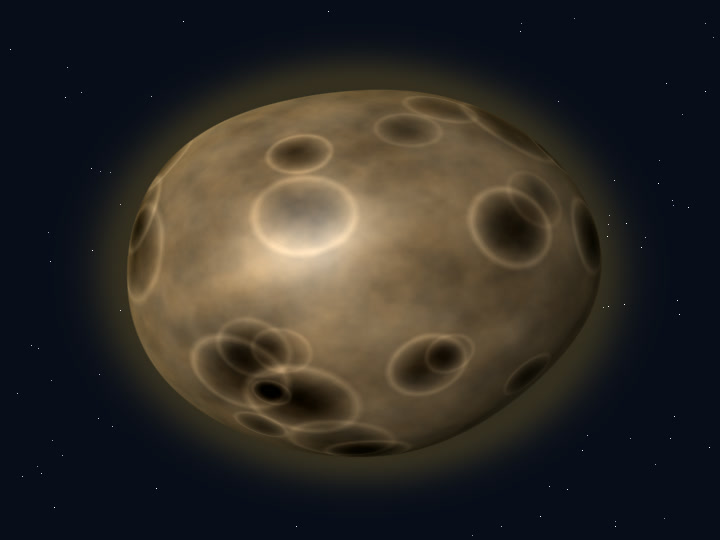
\includegraphics[width=\linewidth,height=4.4cm,keepaspectratio]{imagini/globuri/psyche.jpg}\\[2pt]
{\scriptsize\itshape\color{orbitarMuted} Vedere 3D a corpului ceresc (\textbf{16 Psyche})}
&
\centering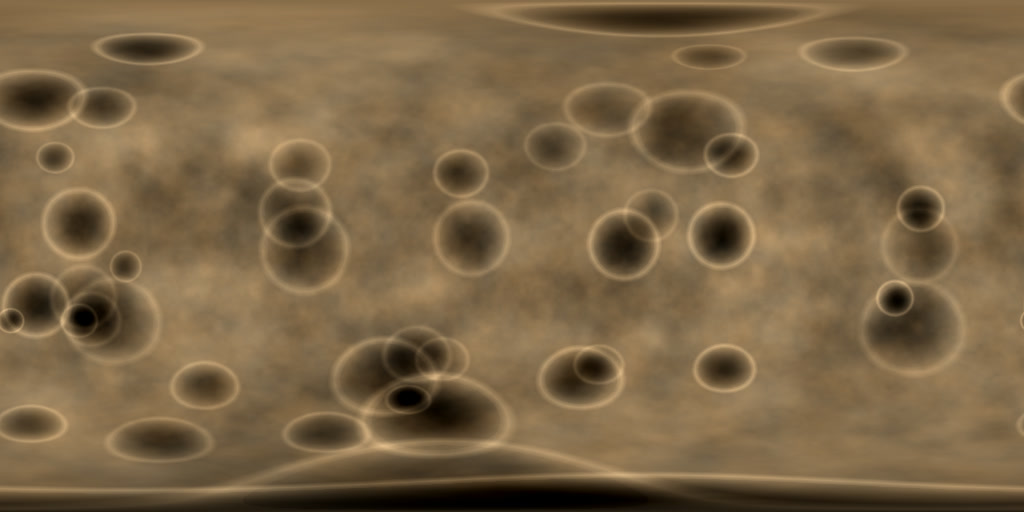
\includegraphics[width=\linewidth,height=4.4cm,keepaspectratio]{imagini/globuri/psyche_map.jpg}\\[2pt]
{\scriptsize\itshape\color{orbitarMuted} Planiglob desfășurat: Harta desfășurată a suprafeței bogate în fier și nichel a asteroidului metalic 16 Psyche.}
\end{tabular}
\end{center}


\begin{tcolorbox}[orbitardata, title={\textbf{Repere esențiale: 16 Psyche}}]
\small
\begin{itemize}[leftmargin=1.4em, itemsep=2pt, topsep=2pt]
  \item \textbf{Clasificare și orbită:} Asteroid \quad$\bullet$\quad \textbf{Distanță:} 2,923 UA ($\approx$ 437 milioane de kilometri)
  \item \textbf{Dimensiuni și masă:} rază medie 111 kilometri \quad$\bullet$\quad masă: 3,80e-6 $\times M_\oplus$
  \item \textbf{Gravitație și regim termic:} 0,015 $\times g_\oplus$ (0,15 m/s$^2$) \quad$\bullet$\quad temperatură medie: -100 $^\circ$C (înclinarea axei: Nespecificată)
  \item \textbf{Ciclu orbital și rotație:} perioadă orbitală (an): 1.823,9 zile ($\approx$ 4,99 ani pământești) \quad$\bullet$\quad rotație (zi): 4,20 ore (0,17 zile pământești) (elemente kepleriene: $a = 2,923$ UA, $e = 0,1340$, $i = 3,09^\circ$, $\Omega = 150,2^\circ$, $\omega = 227,5^\circ$)
  \item \textbf{Durata călătoriei de pe Pământ:} cu viteza luminii ($1c$): \emph{24 de minute}; cu racheta ($50.000$ de kilometri pe oră): \emph{5 ani și 10 luni (sonda Psyche)}; cu avionul ($900$ de kilometri pe oră): \emph{38 de ani}; cu mașina ($100$ de kilometri pe oră): \emph{340 de ani}.
  \item \textbf{Repere de scară și curiozitate:} Oamenii de știință cred că Psyche este inima de metal (nucleul) a unei planete străvechi care și-a pierdut învelișul de piatră! Deoarece nu putem săpa până în nucleul de fier al Pământului nostru, am trimis o sondă spațială să viziteze un nucleu planetar direct în spațiu, pe asteroidul Psyche!
\end{itemize}
\end{tcolorbox}

\subsubsection*{Prezentare generală și profil astrofizic}
Descoperit în 1852 de Annibale de Gasparis, 16 Psyche este cel mai masiv asteroid de tip M (metalic), având un diametru mediu de 222 de kilometri. Conține între 30\% și 60\% fier și nichel metalic amestecat cu silicați săraci în fier. Psyche este un asteroid cu totul special: în timp ce majoritatea asteroizilor sunt din piatră sau gheață, Psyche este făcut în mare parte din metal (fier și nichel)! Oamenii de știință cred că Psyche este inima de metal (nucleul) a unei planete străvechi care și-a pierdut învelișul de piatră!

\subsubsection*{Alcătuirea fizică și structura internă}
Privind în profunzimea sa, alcătuirea fizică este organizată pe mai multe straturi și regiuni distincte, fiecare având un rol bine definit în evoluția și dinamica acestui obiect cosmic. În primul rând se remarcă \textbf{Matrice metalică de fier-nichel}, posibil nucleul expus al unui planetesimal diferențiat timpuriu. În strânsă legătură cu această componentă se află \textbf{Cratere metalice și bazaltice}, două mari depresiuni de impact de aproximativ 90 de kilometri în emisfera sudică. În completarea acestui ansamblu întâlnim \textbf{Regolit mixt metal-silicat}, densitate medie de aproximativ 3,9--4,1 g/cm$^3$.

\subsubsection*{Observații astronomice și istoricul explorării}
Sonda NASA Psyche a fost lansată în octombrie 2023 cu propulsie electrică solară cu efect Hall și va intra pe orbita asteroidului în august 2029. Deoarece nu putem săpa până în nucleul de fier al Pământului nostru, am trimis o sondă spațială să viziteze un nucleu planetar direct în spațiu, pe asteroidul Psyche!

\vspace{6pt}
\begin{tcolorbox}[orbitarquiz, title={\textbf{Întrebare de verificare \#40: 16 Psyche}}]
\textbf{Din ce este alcătuit în proporție ridicată asteroidul 16 Psyche?}
\begin{itemize}[leftmargin=2.2em, itemsep=2pt, topsep=4pt]
  \item[$\square$ \textbf{A.}] Din gheață de metan
  \item[$\square$ \textbf{B.}] Din fier și nichel metalic (și silicați)
  \item[$\square$ \textbf{C.}] Din gaz hidrogen
  \item[$\square$ \textbf{D.}] Din apă lichidă
\end{itemize}
\vspace{2pt}
{\footnotesize\color{orbitarMuted}\textbf{Răspuns corect:} \textbf{B} (Din fier și nichel metalic (și silicați)). \emph{16 Psyche este cel mai mare asteroid de tip M, bogat în fier și nichel, oferind indicii despre cum s-au format nucleele planetelor telurice.}}
\end{tcolorbox}
\clearpage


\subsection{101955 Bennu}
\label{sec:body-bennu}
\vspace{-4pt}
{\large\itshape\color{orbitarAccent} Asteroid în formă de titirez din care NASA a adus mostre pe Pământ}\\[4pt]


\begin{center}
\begin{tabular}{@{}m{0.44\textwidth}@{\hspace{0.03\textwidth}}m{0.51\textwidth}@{}}
\centering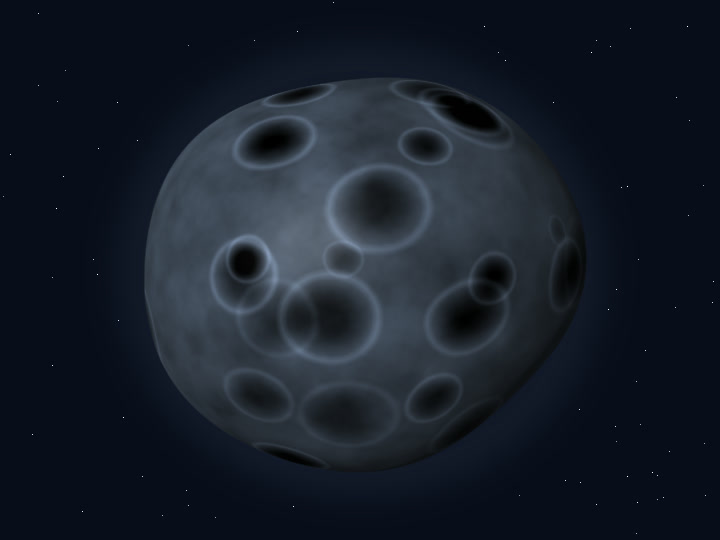
\includegraphics[width=\linewidth,height=4.4cm,keepaspectratio]{imagini/globuri/bennu.jpg}\\[2pt]
{\scriptsize\itshape\color{orbitarMuted} Vedere 3D a corpului ceresc (\textbf{101955 Bennu})}
&
\centering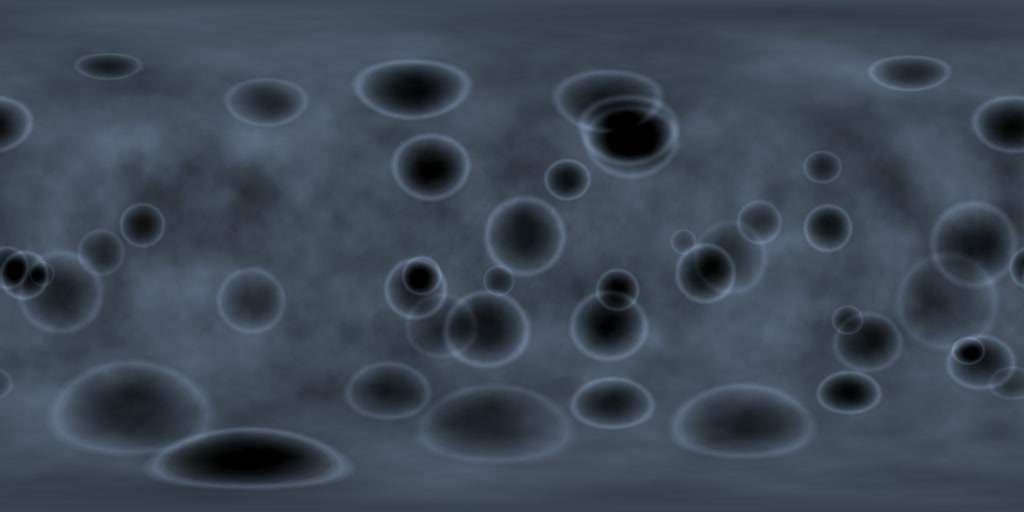
\includegraphics[width=\linewidth,height=4.4cm,keepaspectratio]{imagini/globuri/bennu_map.jpg}\\[2pt]
{\scriptsize\itshape\color{orbitarMuted} Planiglob desfășurat: Harta desfășurată a suprafeței carbonifere întunecate a asteroidului 101955 Bennu.}
\end{tabular}
\end{center}


\begin{tcolorbox}[orbitardata, title={\textbf{Repere esențiale: 101955 Bennu}}]
\small
\begin{itemize}[leftmargin=1.4em, itemsep=2pt, topsep=2pt]
  \item \textbf{Clasificare și orbită:} Asteroid \quad$\bullet$\quad \textbf{Distanță:} 1,126 UA ($\approx$ 168 milioane de kilometri)
  \item \textbf{Dimensiuni și masă:} rază medie 0,245 kilometri \quad$\bullet$\quad masă: 1,20e-11 $\times M_\oplus$
  \item \textbf{Gravitație și regim termic:} Microgravitație / Imponderabilitate ($\approx 0\,g$) \quad$\bullet$\quad temperatură medie: +4 $^\circ$C (înclinarea axei: Nespecificată)
  \item \textbf{Ciclu orbital și rotație:} perioadă orbitală (an): 436,65 zile ($\approx$ 1,20 ani pământești) \quad$\bullet$\quad rotație (zi): 4,30 ore (0,18 zile pământești) (elemente kepleriene: $a = 1,126$ UA, $e = 0,2040$, $i = 6,03^\circ$, $\Omega = 2,1^\circ$, $\omega = 66,2^\circ$)
  \item \textbf{Durata călătoriei de pe Pământ:} cu viteza luminii ($1c$): \emph{1,5 minute}; cu racheta ($50.000$ de kilometri pe oră): \emph{2 ani (OSIRIS-REx)}; cu avionul ($900$ de kilometri pe oră): \emph{3 ani și jumătate}; cu mașina ($100$ de kilometri pe oră): \emph{30 de ani (la apropiere)}.
  \item \textbf{Repere de scară și curiozitate:} Bennu este înalt cam cât o clădire zgârie-nori de 100 de etaje (aproximativ 500 de metri lățime)! Bennu nu este o piatră solidă, ci o grămadă de bolovani și pietriș ținuți împreună de o gravitație minusculă!
\end{itemize}
\end{tcolorbox}

\subsubsection*{Prezentare generală și profil astrofizic}
Asteroid apropiat de Pământ (grupul Apollo) de tip carbonic B, format prin agregarea gravitațională a fragmentelor (\guillemotleft{}rubble-pile\guillemotright{}). Este o capsulă a timpului chimică din primele 10 milioane de ani ale Sistemului Solar. Bennu este un mic asteroid în formă de titirez care trece pe lângă Pământ! O sondă spațială l-a atins și a adus acasă un pumn din pietricelele lui. Bennu este înalt cam cât o clădire zgârie-nori de 100 de etaje (aproximativ 500 de metri lățime)!

\subsubsection*{Alcătuirea fizică și structura internă}
Privind în profunzimea sa, alcătuirea fizică este organizată pe mai multe straturi și regiuni distincte, fiecare având un rol bine definit în evoluția și dinamica acestui obiect cosmic. În primul rând se remarcă \textbf{Structură internă tip \guillemotleft{}grămadă de moloz\guillemotright{} (Rubble Pile)}, cu 20--40\% spații goale în interior și o densitate de doar 1,19 g/cm$^3$. În strânsă legătură cu această componentă se află \textbf{Creastă ecuatorială pronunțată}, îi conferă forma de titirez sau diamant datorită rotației în 4,3 ore. În completarea acestui ansamblu întâlnim \textbf{Regolit bogat în carbon, apă legată în argile și fosfați}, unde 121,6 grame de eșantioane au fost aduse pe Pământ în septembrie 2023.

\subsubsection*{Observații astronomice și istoricul explorării}
Explorat de misiunea NASA OSIRIS-REx (2018--2021), care a colectat mostre din craterul Nightingale și le-a livrat pe Pământ în 2023. Bennu nu este o piatră solidă, ci o grămadă de bolovani și pietriș ținuți împreună de o gravitație minusculă!

\vspace{6pt}
\begin{tcolorbox}[orbitarquiz, title={\textbf{Întrebare de verificare \#41: 101955 Bennu}}]
\textbf{Ce misiune spațială a colectat mostre de pe asteroidul Bennu și le-a adus pe Pământ în 2023?}
\begin{itemize}[leftmargin=2.2em, itemsep=2pt, topsep=4pt]
  \item[$\square$ \textbf{A.}] Voyager 1
  \item[$\square$ \textbf{B.}] OSIRIS-REx
  \item[$\square$ \textbf{C.}] Cassini
  \item[$\square$ \textbf{D.}] Apollo 11
\end{itemize}
\vspace{2pt}
{\footnotesize\color{orbitarMuted}\textbf{Răspuns corect:} \textbf{B} (OSIRIS-REx). \emph{Sonda NASA OSIRIS-REx a colectat peste 120 de grame de regolit carbonic de pe Bennu și a parașutat capsula în deșertul Utah în septembrie 2023.}}
\end{tcolorbox}
\clearpage


\subsection{99942 Apophis}
\label{sec:body-apophis}
\vspace{-4pt}
{\large\itshape\color{orbitarAccent} Asteroidul care va trece în siguranță foarte aproape de Pământ în 2029}\\[4pt]


\begin{center}
\begin{tabular}{@{}m{0.44\textwidth}@{\hspace{0.03\textwidth}}m{0.51\textwidth}@{}}
\centering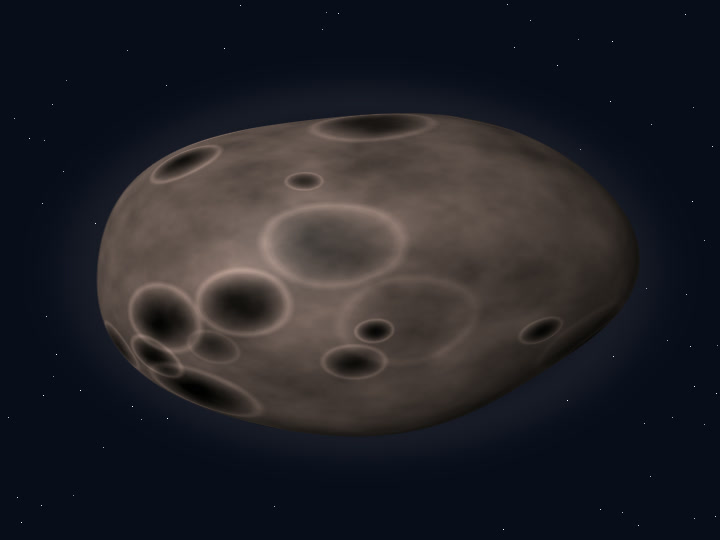
\includegraphics[width=\linewidth,height=4.4cm,keepaspectratio]{imagini/globuri/apophis.jpg}\\[2pt]
{\scriptsize\itshape\color{orbitarMuted} Vedere 3D a corpului ceresc (\textbf{99942 Apophis})}
&
\centering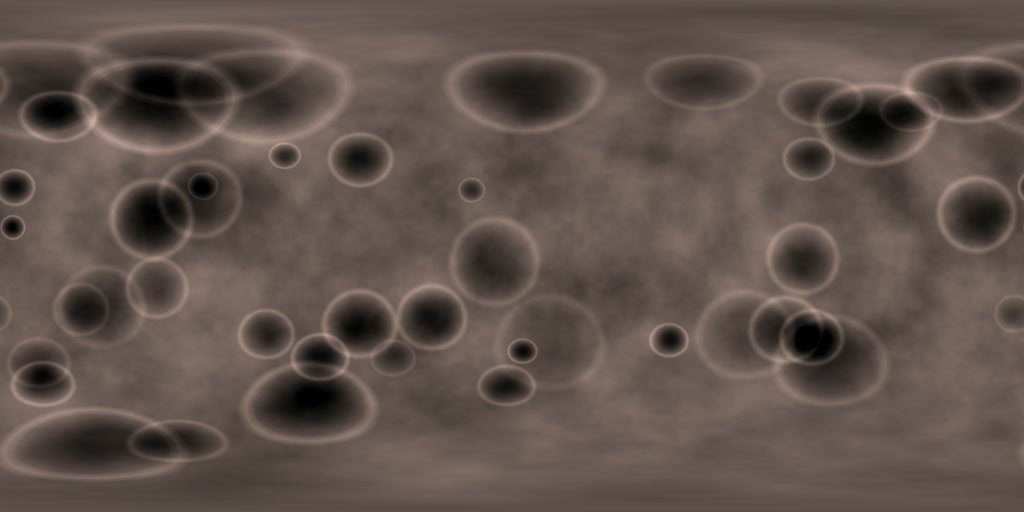
\includegraphics[width=\linewidth,height=4.4cm,keepaspectratio]{imagini/globuri/apophis_map.jpg}\\[2pt]
{\scriptsize\itshape\color{orbitarMuted} Planiglob desfășurat: Harta desfășurată a suprafeței stâncoase a asteroidului din apropierea Pământului 99942 Apophis.}
\end{tabular}
\end{center}


\begin{tcolorbox}[orbitardata, title={\textbf{Repere esențiale: 99942 Apophis}}]
\small
\begin{itemize}[leftmargin=1.4em, itemsep=2pt, topsep=2pt]
  \item \textbf{Clasificare și orbită:} Asteroid \quad$\bullet$\quad \textbf{Distanță:} 0,922 UA ($\approx$ 138 milioane de kilometri)
  \item \textbf{Dimensiuni și masă:} rază medie 0,185 kilometri \quad$\bullet$\quad masă: 4,00e-12 $\times M_\oplus$
  \item \textbf{Gravitație și regim termic:} Microgravitație / Imponderabilitate ($\approx 0\,g$) \quad$\bullet$\quad temperatură medie: +17 $^\circ$C (înclinarea axei: Nespecificată)
  \item \textbf{Ciclu orbital și rotație:} perioadă orbitală (an): 323,6 zile pământești \quad$\bullet$\quad rotație (zi): 30,56 ore (1,27 zile pământești) (elemente kepleriene: $a = 0,922$ UA, $e = 0,1910$, $i = 3,34^\circ$, $\Omega = 204,4^\circ$, $\omega = 126,4^\circ$)
  \item \textbf{Durata călătoriei de pe Pământ:} cu viteza luminii ($1c$): \emph{0,1 secunde la perigeul din 2029}; cu racheta ($50.000$ de kilometri pe oră): \emph{câteva luni pe o traiectorie de întâlnire}; cu avionul ($900$ de kilometri pe oră): \emph{36 de ore (în 2029)}; cu mașina ($100$ de kilometri pe oră): \emph{13 zile la apropierea din 2029}.
  \item \textbf{Repere de scară și curiozitate:} Apophis are mărimea a trei terenuri de fotbal puse cap la cap (aproximativ 370 de metri)! Pe 13 aprilie 2029, Apophis va trece în deplină siguranță la doar 32.000 de kilometri de Pământ, adică mai aproape decât unii sateliți de televiziune!
\end{itemize}
\end{tcolorbox}

\subsubsection*{Prezentare generală și profil astrofizic}
Asteroid de tip S (silicatic) din grupul Aten. Măsurătorile radar de înaltă precizie au confirmat că nu există niciun risc de impact cu Pământul pentru cel puțin următoarea sută de ani, dar survolul din 13 aprilie 2029 va fi o oportunitate științifică unică. Apophis este un asteroid în formă de arahidă care în anul 2029 ne va face o vizită pașnică, trecând pe cer ca o steluță vizibilă cu ochiul liber! Apophis are mărimea a trei terenuri de fotbal puse cap la cap (aproximativ 370 de metri)!

\subsubsection*{Alcătuirea fizică și structura internă}
Privind în profunzimea sa, alcătuirea fizică este organizată pe mai multe straturi și regiuni distincte, fiecare având un rol bine definit în evoluția și dinamica acestui obiect cosmic. În primul rând se remarcă \textbf{Formă bilobată (de arahidă)}, determinată prin imagistică radar de la observatorul Goldstone. În strânsă legătură cu această componentă se află \textbf{Compoziție de condrite ordinare, fier și nichel}, tipică asteroizilor stâncoși de clasă Sq. În completarea acestui ansamblu întâlnim \textbf{Rotație complexă (tumbling)}, unde forțele mareice terestre din 2029 îi vor modifica ușor rotația și orbita.

\subsubsection*{Observații astronomice și istoricul explorării}
Va fi studiat de aproape în 2029 de sonda NASA OSIRIS-APEX (fosta OSIRIS-REx) și de misiunea europeană RAMSES (ESA). Pe 13 aprilie 2029, Apophis va trece în deplină siguranță la doar 32.000 de kilometri de Pământ, adică mai aproape decât unii sateliți de televiziune!

\vspace{6pt}
\begin{tcolorbox}[orbitarquiz, title={\textbf{Întrebare de verificare \#42: 99942 Apophis}}]
\textbf{Ce se va întâmpla pe 13 aprilie 2029 cu asteroidul Apophis?}
\begin{itemize}[leftmargin=2.2em, itemsep=2pt, topsep=4pt]
  \item[$\square$ \textbf{A.}] Va intra pe orbita lui Jupiter
  \item[$\square$ \textbf{B.}] Va trece în deplină siguranță la aproximativ 32.000 de kilometri de Pământ, fiind vizibil cu ochiul liber
  \item[$\square$ \textbf{C.}] Se va topi lângă Soare
  \item[$\square$ \textbf{D.}] Va lovi Luna
\end{itemize}
\vspace{2pt}
{\footnotesize\color{orbitarMuted}\textbf{Răspuns corect:} \textbf{B} (Va trece în deplină siguranță la aproximativ 32.000 de kilometri de Pământ, fiind vizibil cu ochiul liber). \emph{Calculele radar au demonstrat că Apophis va trece fără niciun pericol la aproximativ 32.000 de kilometri de Pământ, oferind astronomilor ocazia rară de a-l studia de aproape.}}
\end{tcolorbox}
\clearpage


% SPDX-License-Identifier: GPL-3.0-or-later
\chapter{Obiecte Lansate de Om: Stații Spațiale, Telescoape, Sonde și Rovere}
\label{chap:misiuni}

Începând cu a doua jumătate a secolului XX, omenirea a trimis în cosmos laboratoare orbitale locuite de astronauți, telescoape spațiale plasate deasupra atmosferei terestre, sonde automate care au explorat fiecare planetă a Sistemului Solar și rovere robotice care analizează rocile de pe Marte. În \textbf{Orbitar} sunt modelate 3D și urmărite orbital \textbf{12 misiuni spațiale emblematice}.

\section*{Unde zboară misiunile spațiale? De la Orbita Joasă (LEO) la Punctul Lagrange L2 și Spațiul Interstelar}

\begin{itemize}[leftmargin=1.5em, itemsep=3pt]
  \item \textbf{Orbita Joasă a Pământului (LEO, \emph{Low Earth Orbit}):} situată între $400$ și $600$ de kilometri altitudine deasupra Pământului. Aici zboară \textbf{Stația Spațială Internațională (ISS)} și \textbf{Telescopul Spațial Hubble} cu o viteză orbitală de aproape $28.000$ de kilometri pe oră, înconjurând globul pământesc o dată la fiecare $90\text{--}95\text{ de minute}$. În \textbf{Orbitar}, poziția lor exactă (latitudine, longitudine, altitudine și viteză) este calculată în timp real prin modelul fizic de perturbații \textbf{SGP4} (\texttt{satellite.js}) din elementele orbitale \textbf{NORAD Two-Line Element (TLE)}.
  \item \textbf{Punctul Lagrange L2 Soare--Pământ ($1{,}5\text{ milioane de kilometri}$ de Pământ):} un punct de echilibru gravitațional și centrifugal situat pe linia Soare--Pământ, în spatele Pământului. Aici orbitează \textbf{Telescopul Spațial James Webb (JWST)} și \textbf{Telescopul Spațial Euclid}, astfel încât scuturile lor termice să blocheze simultan căldura Soarelui, a Pământului și a Lunii!
  \item \textbf{Traiectorii interplanetare și interstelare:} sonde precum \textbf{Parker Solar Probe} (care plonjează în coroana Soarelui), \textbf{Rosetta} (care a însoțit cometa 67P), \textbf{JUICE} (în drum spre lunile înghețate ale lui Jupiter), \textbf{New Horizons} (în Centura Kuiper) și gemenele \textbf{Voyager 1 \& 2} (aflate deja în spațiul interstelar!).
  \item \textbf{Suprafața planetei Marte:} roverele nucleare \textbf{Curiosity} (în Craterul Gale) și \textbf{Perseverance \& elicopterul Ingenuity} (în Craterul Jezero), ancorate în \textbf{Orbitar} direct pe coordonatele lor areografice reale de pe globul rotitor al lui Marte.
\end{itemize}

\begin{center}
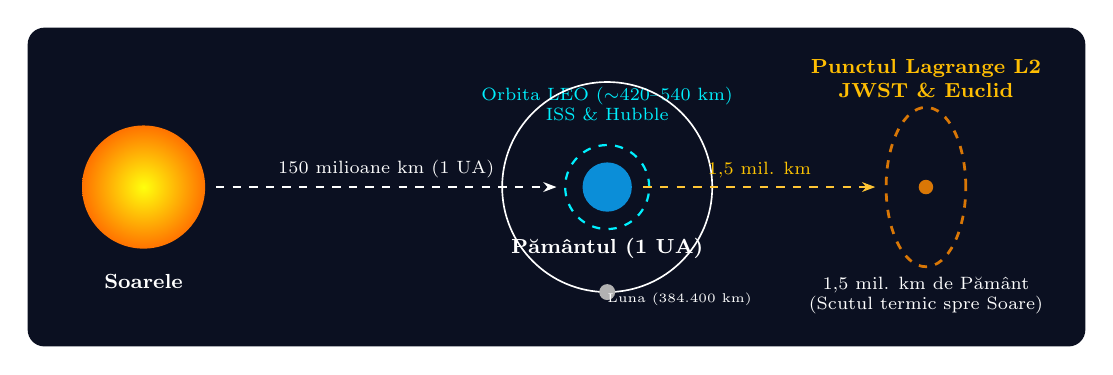
\begin{tikzpicture}[scale=0.92, every node/.style={transform shape}]
  \fill[orbitarSpaceBg, rounded corners=6pt] (-1.2,-2.2) rectangle (13.4,2.2);
  % Soarele
  \shade[inner color=yellow!95!white, outer color=orange!90!red] (0.4,0) circle (0.85cm);
  \node[white, font=\footnotesize\bfseries] at (0.4,-1.3) {Soarele};

  % Pământul
  \fill[cyan!75!blue] (6.8,0) circle (0.34cm);
  \node[white, font=\footnotesize\bfseries] at (6.8,-0.85) {Pământul (1 UA)};

  % Orbita LEO (ISS & Hubble)
  \draw[orbitarCyan, line width=0.8pt, dashed] (6.8,0) circle (0.58cm);
  \node[orbitarCyan, font=\scriptsize, align=center] at (6.8,1.15) {Orbita LEO ($\sim$420--540 km)\\ISS \& Hubble};

  % Orbita Lunii
  \draw[white!40, line width=0.6pt] (6.8,0) circle (1.45cm);
  \fill[gray!60] (6.8,-1.45) circle (0.11cm);
  \node[white!80, font=\tiny] at (7.8,-1.55) {Luna (384.400 km)};

  % Punctul Lagrange L2
  \draw[orbitarAmber, line width=1.0pt, dashed] (11.2,0) ellipse (0.55cm and 1.1cm);
  \fill[orbitarAmber] (11.2,0) circle (0.10cm);
  \node[amber!90!yellow, font=\footnotesize\bfseries, align=center] at (11.2,1.50) {Punctul Lagrange L2\\JWST \& Euclid};
  \node[white!85, font=\scriptsize, align=center] at (11.2,-1.50) {1,5 mil. km de Pământ\\(Scutul termic spre Soare)};

  \draw[-{Stealth}, white!50, dashed] (1.4,0) -- (6.1,0) node[midway, above, font=\scriptsize, text=white!80] {150 milioane km (1 UA)};
  \draw[-{Stealth}, amber!80, dashed] (7.3,0) -- (10.5,0) node[midway, above, font=\scriptsize, text=amber!80!yellow] {1,5 mil. km};
\end{tikzpicture}
\end{center}

\begin{table}[H]
\centering
\small
\caption{Cele 12 misiuni spațiale (stații, telescoape, sonde și rovere) prezente în Orbitar}
\resizebox{\textwidth}{!}{%
\begin{tabular}{@{}lllrr@{}}
\toprule
\textbf{Misiune / Obiect} & \textbf{Tip} & \textbf{Corp central / Regiune} & \textbf{Distanță Soare} & \textbf{Temp. operare} \\
\midrule
Stația Spațială Internațională (ISS) & Stație Spațială Orbitală & Pământul & 1,00 UA & 21$^\circ$C \\
Telescopul Spațial Hubble & Telescop Spațial & Pământul & 1,00 UA & 15$^\circ$C \\
Telescopul Spațial James Webb (JWST) & Telescop Spațial & Pământul & 1,01 UA & -233$^\circ$C \\
Telescopul Spațial Euclid & Telescop Spațial & Pământul & 1,01 UA & -190$^\circ$C \\
Voyager 1 & Sondă Interplanetară & Soarele (Heliocentric) & 165,00 UA & -195$^\circ$C \\
Voyager 2 & Sondă Interplanetară & Soarele (Heliocentric) & 138,00 UA & -195$^\circ$C \\
New Horizons & Sondă Interplanetară & Soarele (Heliocentric) & 60,20 UA & -210$^\circ$C \\
Parker Solar Probe & Sondă Interplanetară & Soarele (Heliocentric) & 0,25 UA & 1.370$^\circ$C \\
Rosetta \& Philae & Sondă Interplanetară & Soarele (Heliocentric) & 3,46 UA & -70$^\circ$C \\
JUICE (Jupiter Icy Moons Explorer) & Sondă Interplanetară & Soarele (Heliocentric) & 3,10 UA & -150$^\circ$C \\
Perseverance \& Ingenuity & Rover Planetar & Marte & 1,52 UA & -63$^\circ$C \\
Curiosity (Mars Science Laboratory) & Rover Planetar & Marte & 1,52 UA & -63$^\circ$C \\
\bottomrule
\end{tabular}%
}
\end{table}

\begin{tcolorbox}[orbitardata, title={\textbf{Propagare Orbitală SGP4 100\% Offline în Orbitar (\texttt{public/data/tle-iss.json})}}]
Pentru a calcula poziția deasupra continentelor fără a depinde de internet, \textbf{Orbitar} integrează algoritmul astrodinamic \textbf{SGP4} cu seturile oficiale \textbf{NORAD Two-Line Element (TLE)}:
\begin{itemize}[leftmargin=1.4em, itemsep=3pt]
  \item \textbf{ISS (ZARYA), Stația Spațială Internațională (NORAD ID 25544):} altitudine nominală aproximativ 418,5 de kilometri, viteză orbitală aproximativ 27.580 de kilometri pe oră ($15{,}49\text{ orbite/zi}$, înclinație $51{,}64^\circ$).\\
  {\scriptsize\texttt{1 25544U 98067A   24305.51234567  .00016717  00000-0  30124-3 0  9995}}\\
  {\scriptsize\texttt{2 25544  51.6416 247.4627 0006703 130.5360 325.0288 15.49815350479612}}
  \item \textbf{HST, Telescopul Spațial Hubble (NORAD ID 20580):} altitudine nominală aproximativ 535,2 de kilometri, viteză orbitală aproximativ 27.310 de kilometri pe oră ($15{,}12\text{ orbite/zi}$, înclinație $28{,}47^\circ$).\\
  {\scriptsize\texttt{1 20580U 90037B   24305.48123456  .00001842  00000-0  96145-4 0  9991}}\\
  {\scriptsize\texttt{2 20580  28.4698 118.2341 0002640 284.1290  75.9124 15.12498120891245}}
\end{itemize}
\end{tcolorbox}

\begin{tcolorbox}[orbitarjunior, title={\textbf{Discul de Aur Voyager (1977) și Salutul în Limba Română din Spațiul Interstelar}}]
La bordul ambelor sonde \textbf{Voyager 1} și \textbf{Voyager 2} (lansate în august--septembrie 1977) se află \textbf{Discul de Aur (\emph{Voyager Golden Record})}, un disc de cupru placat cu aur cu diametrul de $30$ de centimetri, conceput de o comisie condusă de astronomul \textbf{Carl Sagan} ca o „sticlă cu mesaj în oceanul cosmic”. Discul conține 115 imagini codate analogic, sunete ale naturii terestre, 90 de minute de muzică (Bach, Beethoven, Mozart, folclor mondial) și \textbf{saluturi rostite în 55 de limbi ale Pământului}.\\[4pt]
Printre cele 55 de limbi se află și \textbf{limba română}, cu mesajul rostit de \textbf{Sanda Huffman}:\\
\begin{center}
{\Large\bfseries\color{orbitarDeepBlue}„Salutări la toată lumea!”}
\end{center}
În aplicația \textbf{Orbitar}, când selectezi \emph{Voyager 1} sau \emph{Voyager 2}, poți asculta acest salut istoric direct din caseta dedicată a \textbf{Laboratorului Orbitar}!
\end{tcolorbox}

\begin{tcolorbox}[orbitarcadet, title={\textbf{Atlasul Reperelor Geografice și al Roverelor de pe Marte în Orbitar (\texttt{SurfaceMarkers.ts})}}]
Pe globul 3D al planetei \textbf{Marte}, aplicația \textbf{Orbitar} afișează 6 pini geografici interactivi care marchează rovere active, cratere lacustre fosile și cel mai înalt vulcan din Sistemul Solar:
\begin{enumerate}[leftmargin=1.5em, itemsep=3pt]
  \item \textbf{Roverul Perseverance \& Elicopterul Ingenuity ($18{,}38^\circ\text{ N}, 77{,}58^\circ\text{ E}$, 2021):} laborator astrobiologic mobil de $1.025$ de kilograme amartizat în Craterul Jezero; caută biosemnături străvechi, sigilează tuburi cu mostre de rocă, a produs oxigen pe Marte prin experimentul \emph{MOXIE} și a adus elicopterul \emph{Ingenuity} (care a realizat 72 de zboruri propulsate!).
  \item \textbf{Roverul Curiosity, Mars Science Laboratory ($4{,}58^\circ\text{ S}, 137{,}44^\circ\text{ E}$, 2012):} rover nuclear de $899$ de kilograme care explorează Craterul Gale și urcă pe straturile Muntelui Sharp; a demonstrat că Marte a avut râuri și lacuri cu apă dulce capabile să susțină viața microbiană.
  \item \textbf{Craterul Jezero ($18{,}85^\circ\text{ N}, 77{,}52^\circ\text{ E}$):} crater de impact cu diametrul de $45$ de kilometri care, acum peste $3{,}5\text{ miliarde de ani}$, adăpostea un lac adânc alimentat de un râu, a cărui deltă fluvială fosilă păstrează sedimente de argilă și carbonați.
  \item \textbf{Craterul Gale \& Muntele Sharp / Aeolis Mons ($5{,}4^\circ\text{ S}, 137{,}8^\circ\text{ E}$):} bazin sedimentar cu diametrul de $154$ de kilometri în centrul căruia se înalță \emph{Aeolis Mons} ($5.500$ de metri altitudine), ale cărui straturi de argile și sulfați arată tranziția lui Marte de la o planetă caldă și umedă la un deșert înghețat.
  \item \textbf{Vulcanul Olympus Mons ($18{,}65^\circ\text{ N}, 133{,}8^\circ\text{ V}$):} vulcan-scut gigantic din regiunea Tharsis, cu înălțimea de $21{,}9$ kilometri (de aproape trei ori mai înalt decât Muntele Everest de pe Pământ!) și o bază cu lățimea de $600$ de kilometri, comparabilă cu suprafața României!
  \item \textbf{Chryse Planitia, Sonda Viking 1 ($22{,}27^\circ\text{ N}, 47{,}95^\circ\text{ V}$, 20 iulie 1976):} prima sondă din istorie care a amartizat cu succes și a transmis fotografii color direct de pe solul marțian, funcționând timp de peste 6 ani.
\end{enumerate}
\end{tcolorbox}

\clearpage

\section{Stația Spațială Internațională (ISS)}
\label{sec:body-iss}
\vspace{-4pt}
{\large\itshape\color{orbitarAccent} Laboratorul științific locuit permanent pe orbita joasă a Pământului}\\[4pt]


\begin{center}
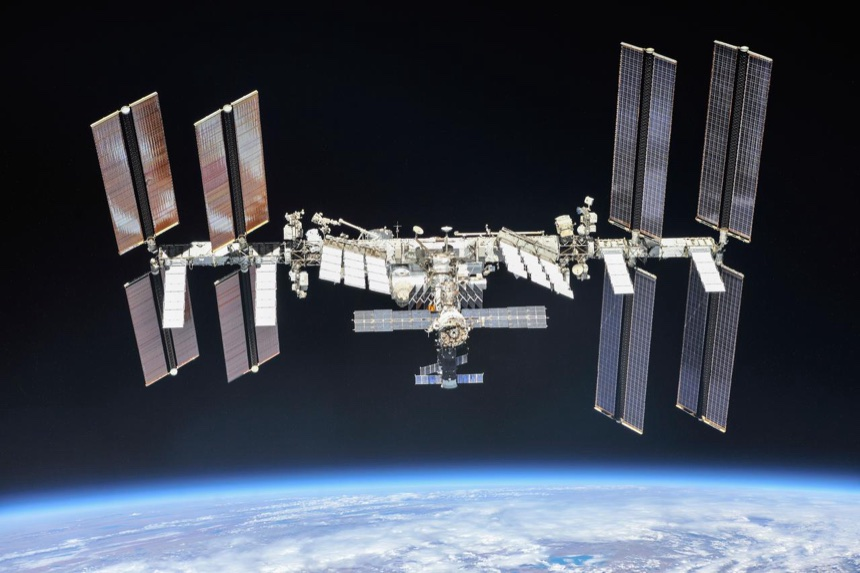
\includegraphics[width=0.78\textwidth,height=5.6cm,keepaspectratio]{../public/textures/nasa/iss.jpg}\\[3pt]
{\footnotesize\itshape\color{orbitarMuted} Fotografie reală NASA (ISS056E201248): Stația Spațială Internațională pe orbita joasă a Pământului (aproximativ 420 de kilometri altitudine).}
\end{center}


\begin{tcolorbox}[orbitardata, title={\textbf{Repere esențiale: Stația Spațială Internațională (ISS)}}]
\small
\begin{itemize}[leftmargin=1.4em, itemsep=2pt, topsep=2pt]
  \item \textbf{Clasificare și orbită:} Stație Spațială Orbitală (orbitează în jurul: \textbf{Pământul}) \quad$\bullet$\quad \textbf{Distanță:} 1,000 UA ($\approx$ 150 milioane de kilometri)
  \item \textbf{Dimensiuni și masă:} anvergură de aproximativ 55 de metri \quad$\bullet$\quad masă: Vehicul spațial artificial
  \item \textbf{Gravitație și regim termic:} Microgravitație / Imponderabilitate ($\approx 0\,g$) \quad$\bullet$\quad temperatură medie: +21 $^\circ$C
  \item \textbf{Ciclu orbital și rotație:} perioadă orbitală (an): 0,064 zile pământești \quad$\bullet$\quad rotație (zi): 1,54 ore (0,06 zile pământești)
  \item \textbf{Durata călătoriei de pe Pământ:} cu viteza luminii ($1c$): \emph{0,0014 secunde}; cu racheta ($50.000$ de kilometri pe oră): \emph{8 minute până pe orbită (și 4--24 ore până la andocare)}; cu avionul ($900$ de kilometri pe oră): \emph{30 de minute (dacă un avion ar putea zbura în sus)}; cu mașina ($100$ de kilometri pe oră): \emph{4 ore pe verticală (se află la aproximativ 410 kilometri altitudine)}.
  \item \textbf{Repere de scară și curiozitate:} ISS este mare cât un teren de fotbal, cu aripi strălucitoare de panouri solare! ISS zboară atât de repede (28.000 kilometri pe oră) încât astronauții văd 16 răsărituri și 16 apusuri de Soare în fiecare zi!
\end{itemize}
\end{tcolorbox}

\vspace{4pt}
\noindent\textbf{Prezentare generală și profil astrofizic.} Construită începând din 1998 prin cooperarea dintre NASA, ESA, Roscosmos, JAXA și CSA, ISS orbitează la aproximativ 410 kilometri altitudine cu o viteză de 7,66 kilometri pe secundă. Este locuită continuu de echipaje umane din noiembrie 2000. Stația Spațială Internațională este o casă și un laborator uriaș care zboară deasupra Pământului! Acolo astronauții plutesc în imponderabilitate și fac experimente pentru toată omenirea. ISS este mare cât un teren de fotbal, cu aripi strălucitoare de panouri solare!

\medskip
\noindent\textbf{Arhitectura tehnică și instrumentele științifice de la bord.} Din punct de vedere constructiv și ingineresc, vehiculul spațial reunește mai multe subsisteme și instrumente științifice de înaltă precizie, proiectate să funcționeze în condițiile extreme ale spațiului cosmic. În primul rând se remarcă \textbf{Module presurizate (Columbus, Destiny, Kibo, Zvezda)}, laboratoare de biologie, fizică a fluidelor, medicină spațială și observații terestre. În strânsă legătură cu această componentă se află \textbf{Grinda centrală (Integrated Truss Structure) și Panourile Solare}, 8 aripi fotovoltaice uriașe care generează peste 120 kW de energie electrică. În completarea acestui ansamblu întâlnim \textbf{Brațul robotic Canadarm2 și Cupola}, braț de manipulare de 17 metri și fereastra panoramică cu 7 geamuri îndreptată spre Pământ.

\medskip
\noindent\textbf{Observații astronomice și istoricul explorării.} Peste 270 de astronauți din peste 20 de țări au lucrat la bordul ISS în mai mult de două decenii de prezență umană neîntreruptă în spațiu. ISS zboară atât de repede (28.000 kilometri pe oră) încât astronauții văd 16 răsărituri și 16 apusuri de Soare în fiecare zi!

\vspace{6pt}
\begin{tcolorbox}[orbitarquiz, title={\textbf{Întrebare de verificare \#35: Stația Spațială Internațională (ISS)}}]
\textbf{În cât timp face Stația Spațială Internațională o tură completă în jurul Pământului?}
\begin{itemize}[leftmargin=2.2em, itemsep=2pt, topsep=4pt]
  \item[$\square$ \textbf{A.}] În 24 de ore
  \item[$\square$ \textbf{B.}] În aproximativ 92 de minute
  \item[$\square$ \textbf{C.}] În 7 zile
  \item[$\square$ \textbf{D.}] Într-o lună
\end{itemize}
\vspace{2pt}
{\footnotesize\color{orbitarMuted}\textbf{Răspuns corect:} \textbf{B} (În aproximativ 92 de minute). \emph{La viteza orbitală de aproximativ 28.000 kilometri pe oră, ISS înconjoară întregul Pământ în aproximativ 92 de minute ( de aproape 16 ori pe zi).}}
\end{tcolorbox}
\clearpage


\section{Telescopul Spațial Hubble}
\label{sec:body-hubble}
\vspace{-4pt}
{\large\itshape\color{orbitarAccent} Ochiul cosmic de pe orbita Pământului care a fotografiat Universul timp de peste 30 de ani}\\[4pt]


\begin{center}
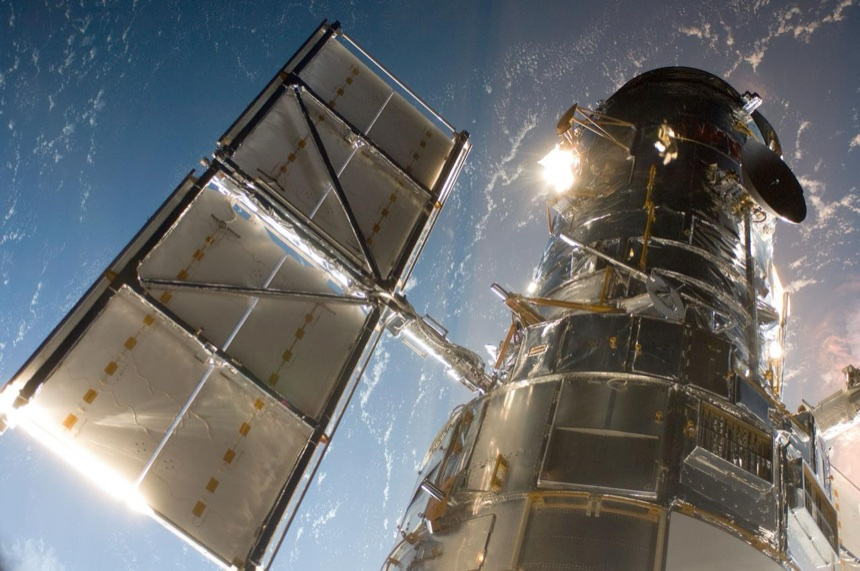
\includegraphics[width=0.78\textwidth,height=5.6cm,keepaspectratio]{../public/textures/nasa/hubble.jpg}\\[3pt]
{\footnotesize\itshape\color{orbitarMuted} Fotografie reală NASA (STS-125): Telescopul Spațial Hubble pe orbită deasupra Pământului.}
\end{center}


\begin{tcolorbox}[orbitardata, title={\textbf{Repere esențiale: Telescopul Spațial Hubble}}]
\small
\begin{itemize}[leftmargin=1.4em, itemsep=2pt, topsep=2pt]
  \item \textbf{Clasificare și orbită:} Telescop Spațial (orbitează în jurul: \textbf{Pământul}) \quad$\bullet$\quad \textbf{Distanță:} 1,000 UA ($\approx$ 150 milioane de kilometri)
  \item \textbf{Dimensiuni și masă:} anvergură de aproximativ 7 metri \quad$\bullet$\quad masă: Vehicul spațial artificial
  \item \textbf{Gravitație și regim termic:} Microgravitație / Imponderabilitate ($\approx 0\,g$) \quad$\bullet$\quad temperatură medie: +15 $^\circ$C
  \item \textbf{Ciclu orbital și rotație:} perioadă orbitală (an): 0,066 zile pământești \quad$\bullet$\quad rotație (zi): 1,58 ore (0,07 zile pământești)
  \item \textbf{Durata călătoriei de pe Pământ:} cu viteza luminii ($1c$): \emph{0,0018 secunde}; cu racheta ($50.000$ de kilometri pe oră): \emph{8 minute și jumătate}; cu avionul ($900$ de kilometri pe oră): \emph{38 de minute}; cu mașina ($100$ de kilometri pe oră): \emph{5 ore și jumătate (540 de kilometri altitudine)}.
  \item \textbf{Repere de scară și curiozitate:} Hubble are mărimea unui autobuz școlar argintiu cu două aripi solare! Hubble are o vedere atât de precisă încât ar putea zări lumina unui licurici aflat la peste 10.000 de kilometri distanță!
\end{itemize}
\end{tcolorbox}

\vspace{4pt}
\noindent\textbf{Prezentare generală și profil astrofizic.} Lansat la 24 aprilie 1990 de naveta Discovery (NASA/ESA), Hubble observă în spectrul vizibil, ultraviolet și infraroșu apropiat de la o altitudine de aproximativ 535 de kilometri, fără distorsiunile atmosferei terestre. Telescopul Hubble este un aparat foto uriaș care plutește în spațiu, deasupra norilor Pământului, și ne trimite cele mai colorate imagini cu nebuloase, stele și galaxii! Hubble are mărimea unui autobuz școlar argintiu cu două aripi solare!

\medskip
\noindent\textbf{Arhitectura tehnică și instrumentele științifice de la bord.} Din punct de vedere constructiv și ingineresc, vehiculul spațial reunește mai multe subsisteme și instrumente științifice de înaltă precizie, proiectate să funcționeze în condițiile extreme ale spațiului cosmic. În primul rând se remarcă \textbf{Oglinda primară Ritchey-Chrétien (2,4 metri diametru)}, șlefuită cu precizie nanometrică și acoperită cu un strat reflectorizant de aluminiu și fluorură de magneziu. În strânsă legătură cu această componentă se află \textbf{Camerele WFC3 și ACS}, instrumente de imagistică cu câmp larg care au realizat celebrele imagini \guillemotleft{}Hubble Ultra-Deep Field\guillemotright{}. În completarea acestui ansamblu întâlnim \textbf{Giroscoape și roți de reacție}, care mențin telescopul îndreptat spre ținte cosmice fără să folosească propulsor chimic care ar murdări oglinda.

\medskip
\noindent\textbf{Observații astronomice și istoricul explorării.} A fost reparat și modernizat direct pe orbită de astronauți în 5 misiuni ale navetelor spațiale (1993--2009), realizând peste 1,6 milioane de observații. Hubble are o vedere atât de precisă încât ar putea zări lumina unui licurici aflat la peste 10.000 de kilometri distanță!

\vspace{6pt}
\begin{tcolorbox}[orbitarquiz, title={\textbf{Întrebare de verificare \#36: Telescopul Spațial Hubble}}]
\textbf{De ce vede Telescopul Hubble mult mai clar decât multe telescoape de pe Pământ?}
\begin{itemize}[leftmargin=2.2em, itemsep=2pt, topsep=4pt]
  \item[$\square$ \textbf{A.}] Pentru că este mult mai aproape de stele
  \item[$\square$ \textbf{B.}] Pentru că se află în spațiu, deasupra atmosferei turbulente a Pământului
  \item[$\square$ \textbf{C.}] Pentru că are o lanternă uriașă
  \item[$\square$ \textbf{D.}] Pentru că se află pe Lună
\end{itemize}
\vspace{2pt}
{\footnotesize\color{orbitarMuted}\textbf{Răspuns corect:} \textbf{B} (Pentru că se află în spațiu, deasupra atmosferei turbulente a Pământului). \emph{Atmosfera Pământului estompează și face stelele să \guillemotleft{}pâlpâie\guillemotright{} (scintilație); aflat în vidul spațial la 535 de kilometri altitudine, Hubble obține imagini de o claritate excepțională.}}
\end{tcolorbox}
\clearpage


\section{Telescopul Spațial James Webb (JWST)}
\label{sec:body-jwst}
\vspace{-4pt}
{\large\itshape\color{orbitarAccent} Cel mai puternic observator spațial în infraroșu, cu oglindă aurită de tip fagure}\\[4pt]


\begin{center}
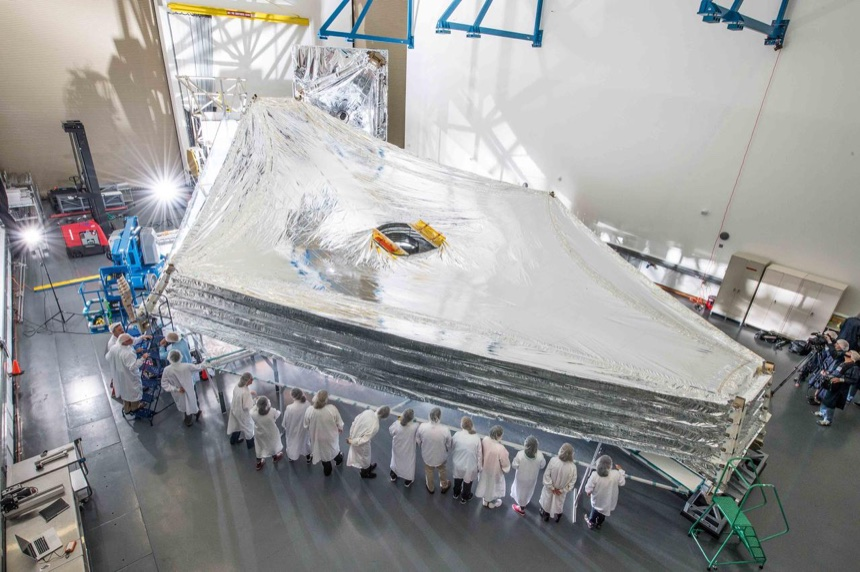
\includegraphics[width=0.78\textwidth,height=5.6cm,keepaspectratio]{../public/textures/nasa/jwst.jpg}\\[3pt]
{\footnotesize\itshape\color{orbitarMuted} Imagine oficială NASA/GSFC: Telescopul Spațial James Webb cu oglinda din 18 segmente hexagonale aurii și scutul termic în 5 straturi.}
\end{center}


\begin{tcolorbox}[orbitardata, title={\textbf{Repere esențiale: Telescopul Spațial James Webb (JWST)}}]
\small
\begin{itemize}[leftmargin=1.4em, itemsep=2pt, topsep=2pt]
  \item \textbf{Clasificare și orbită:} Telescop Spațial (orbitează în jurul: \textbf{Pământul}) \quad$\bullet$\quad \textbf{Distanță:} 1,010 UA ($\approx$ 151 milioane de kilometri)
  \item \textbf{Dimensiuni și masă:} anvergură de aproximativ 11 metri \quad$\bullet$\quad masă: Vehicul spațial artificial
  \item \textbf{Gravitație și regim termic:} Microgravitație / Imponderabilitate ($\approx 0\,g$) \quad$\bullet$\quad temperatură medie: -233 $^\circ$C
  \item \textbf{Ciclu orbital și rotație:} perioadă orbitală (an): 182,62 zile pământești \quad$\bullet$\quad rotație (zi): 24,00 ore (1,00 zile pământești) (elemente kepleriene: $a = 1,010$ UA, $e = 0,0167$, $i = 0,50^\circ$, $\Omega = 0,0^\circ$, $\omega = 102,9^\circ$)
  \item \textbf{Durata călătoriei de pe Pământ:} cu viteza luminii ($1c$): \emph{5 secunde față de Pământ}; cu racheta ($50.000$ de kilometri pe oră): \emph{29 de zile (până în punctul Lagrange L2)}; cu avionul ($900$ de kilometri pe oră): \emph{2 luni și jumătate}; cu mașina ($100$ de kilometri pe oră): \emph{1,7 ani (1,5 milioane de kilometri față de Pământ)}.
  \item \textbf{Repere de scară și curiozitate:} Oglinda lui arată ca un fagure de miere uriaș, iar sub el are o umbrelă de soare cu 5 straturi cât un teren de tenis! Pentru a încăpea în racheta Ariane 5, telescopul a fost împachetat ca un origami și s-a despăturit singur în spațiu!
\end{itemize}
\end{tcolorbox}

\vspace{4pt}
\noindent\textbf{Prezentare generală și profil astrofizic.} Dezvoltat de NASA, ESA și CSA și lansat la 25 decembrie 2021, JWST orbitează în jurul punctului Lagrange L2 Soare--Pământ (la 1,5 milioane de kilometri de Pământ). Observă în infraroșu primele galaxii formate după Big Bang și analizează atmosferele exoplanetelor. Telescopul James Webb este o bijuterie cosmică cu o oglindă mare cât o casă, formată din 18 plăci hexagonale acoperite cu aur adevărat! Oglinda lui arată ca un fagure de miere uriaș, iar sub el are o umbrelă de soare cu 5 straturi cât un teren de tenis!

\medskip
\noindent\textbf{Arhitectura tehnică și instrumentele științifice de la bord.} Din punct de vedere constructiv și ingineresc, vehiculul spațial reunește mai multe subsisteme și instrumente științifice de înaltă precizie, proiectate să funcționeze în condițiile extreme ale spațiului cosmic. În primul rând se remarcă \textbf{Oglinda primară segmentată (6,5 metri diametru)}, 18 segmente hexagonale din beriliu acoperite cu un strat microscopic de aur pentru reflexie maximă în infraroșu. În strânsă legătură cu această componentă se află \textbf{Scutul termic în 5 straturi (Kapton)}, care menține instrumentele la -233 $^\circ$C (40 K), blocând căldura Soarelui, a Pământului și a Lunii. În completarea acestui ansamblu întâlnim \textbf{Instrumentele NIRCam, NIRSpec, MIRI și FGS/NIRISS}, camere și spectrografe capabile să străpungă norii de praf cosmic și să detecteze apă și CO$_2$ pe exoplanete.

\medskip
\noindent\textbf{Observații astronomice și istoricul explorării.} Lansat din Kourou cu o rachetă europeană Ariane 5 în decembrie 2021; a transmis primele imagini științifice revoluționare în iulie 2022. Pentru a încăpea în racheta Ariane 5, telescopul a fost împachetat ca un origami și s-a despăturit singur în spațiu!

\vspace{6pt}
\begin{tcolorbox}[orbitarquiz, title={\textbf{Întrebare de verificare \#37: Telescopul Spațial James Webb (JWST)}}]
\textbf{Din câte segmente hexagonale aurite este alcătuită oglinda principală a Telescopului James Webb?}
\begin{itemize}[leftmargin=2.2em, itemsep=2pt, topsep=4pt]
  \item[$\square$ \textbf{A.}] 6 segmente
  \item[$\square$ \textbf{B.}] 18 segmente
  \item[$\square$ \textbf{C.}] 100 de segmente
  \item[$\square$ \textbf{D.}] Un singur bloc de sticlă
\end{itemize}
\vspace{2pt}
{\footnotesize\color{orbitarMuted}\textbf{Răspuns corect:} \textbf{B} (18 segmente). \emph{Oglinda de 6,5 metri a JWST este formată din 18 segmente hexagonale din beriliu aurit care s-au depliat și aliniat la nivel nanometric în spațiu.}}
\end{tcolorbox}
\clearpage


\section{Telescopul Spațial Euclid}
\label{sec:body-euclid}
\vspace{-4pt}
{\large\itshape\color{orbitarAccent} Cartograful european al Universului Întunecat (în punctul Lagrange L2)}\\[4pt]


\begin{center}
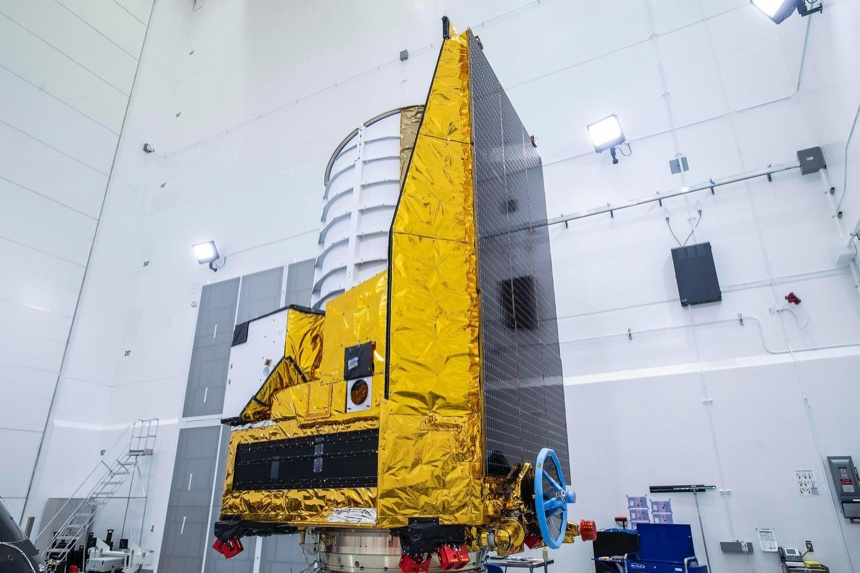
\includegraphics[width=0.78\textwidth,height=5.6cm,keepaspectratio]{../public/textures/nasa/euclid.jpg}\\[3pt]
{\footnotesize\itshape\color{orbitarMuted} Fotografie oficială NASA/ESA (PIA25783): Telescopul Spațial Euclid pentru cartografierea materiei și energiei întunecate.}
\end{center}


\begin{tcolorbox}[orbitardata, title={\textbf{Repere esențiale: Telescopul Spațial Euclid}}]
\small
\begin{itemize}[leftmargin=1.4em, itemsep=2pt, topsep=2pt]
  \item \textbf{Clasificare și orbită:} Telescop Spațial (orbitează în jurul: \textbf{Pământul}) \quad$\bullet$\quad \textbf{Distanță:} 1,010 UA ($\approx$ 151 milioane de kilometri)
  \item \textbf{Dimensiuni și masă:} anvergură de aproximativ 2 metri \quad$\bullet$\quad masă: Vehicul spațial artificial
  \item \textbf{Gravitație și regim termic:} Microgravitație / Imponderabilitate ($\approx 0\,g$) \quad$\bullet$\quad temperatură medie: -190 $^\circ$C
  \item \textbf{Ciclu orbital și rotație:} perioadă orbitală (an): 182,62 zile pământești \quad$\bullet$\quad rotație (zi): 24,00 ore (1,00 zile pământești) (elemente kepleriene: $a = 1,010$ UA, $e = 0,0180$, $i = 1,20^\circ$, $\Omega = 18,0^\circ$, $\omega = 98,0^\circ$)
  \item \textbf{Durata călătoriei de pe Pământ:} cu viteza luminii ($1c$): \emph{5 secunde față de Pământ}; cu racheta ($50.000$ de kilometri pe oră): \emph{30 de zile până în L2}; cu avionul ($900$ de kilometri pe oră): \emph{2 luni și jumătate}; cu mașina ($100$ de kilometri pe oră): \emph{1,7 ani (1,5 milioane de kilometri de Pământ)}.
  \item \textbf{Repere de scară și curiozitate:} Dacă James Webb este o lupă super-puternică ce privește un singur detaliu, Euclid este un aparat foto panoramic care cuprinde o bucată uriașă de cer dintr-odată! Numele lui vine de la Euclid din Alexandria, matematicianul antic numit \guillemotleft{}părintele geometriei\guillemotright{}!
\end{itemize}
\end{tcolorbox}

\vspace{4pt}
\noindent\textbf{Prezentare generală și profil astrofizic.} Lansat în iulie 2023 de ESA, Euclid operează în punctul Lagrange L2 pentru a investiga natura materiei întunecate și a energiei întunecate, cartografiind distribuția tridimensională a miliarde de galaxii pe o distanță de 10 miliarde de ani-lumină. Euclid este telescopul Agenției Spațiale Europene (ESA) trimis să deseneze cea mai mare hartă 3D a miliarde de galaxii din Univers! Dacă James Webb este o lupă super-puternică ce privește un singur detaliu, Euclid este un aparat foto panoramic care cuprinde o bucată uriașă de cer dintr-odată!

\medskip
\noindent\textbf{Arhitectura tehnică și instrumentele științifice de la bord.} Din punct de vedere constructiv și ingineresc, vehiculul spațial reunește mai multe subsisteme și instrumente științifice de înaltă precizie, proiectate să funcționeze în condițiile extreme ale spațiului cosmic. În primul rând se remarcă \textbf{Telescop Korsch din carbură de siliciu (1,2 metri)}, material ceramic ultra-stabil termic care previne orice deformare optică. În strânsă legătură cu această componentă se află \textbf{Camera în spectru vizibil VIS (600 megapixeli)}, care măsoară cu precizie extremă forma galaxiilor și efectul de lentilă gravitațională slabă. În completarea acestui ansamblu întâlnim \textbf{Spectrometrul și fotometrul în infraroșu apropiat NISP}, care determină distanța (redshift-ul) fiecărei galaxii observate.

\medskip
\noindent\textbf{Observații astronomice și istoricul explorării.} Lansat la 1 iulie 2023; primele sale imagini cosmice (\guillemotleft{}Early Release Observations\guillemotright{}) au dezvăluit roiul Perseus și mii de galaxii necunoscute anterior. Numele lui vine de la Euclid din Alexandria, matematicianul antic numit \guillemotleft{}părintele geometriei\guillemotright{}!

\vspace{6pt}
\begin{tcolorbox}[orbitarquiz, title={\textbf{Întrebare de verificare \#38: Telescopul Spațial Euclid}}]
\textbf{Care este obiectivul științific principal al misiunii europene Euclid?}
\begin{itemize}[leftmargin=2.2em, itemsep=2pt, topsep=4pt]
  \item[$\square$ \textbf{A.}] Asolizarea pe Venus
  \item[$\square$ \textbf{B.}] Realizarea unei hărți 3D a miliarde de galaxii pentru a studia materia și energia întunecată
  \item[$\square$ \textbf{C.}] Fotografierea petelor solare
  \item[$\square$ \textbf{D.}] Colectarea de roci lunare
\end{itemize}
\vspace{2pt}
{\footnotesize\color{orbitarMuted}\textbf{Răspuns corect:} \textbf{B} (Realizarea unei hărți 3D a miliarde de galaxii pentru a studia materia și energia întunecată). \emph{Euclid măsoară geometria la scară mare a Universului pentru a înțelege cum materia întunecată și energia întunecată îi modelează expansiunea.}}
\end{tcolorbox}
\clearpage


\section{Voyager 1}
\label{sec:body-voyager1}
\vspace{-4pt}
{\large\itshape\color{orbitarAccent} Cel mai îndepărtat obiect creat de om, călătorind în spațiul interstelar}\\[4pt]


\begin{center}
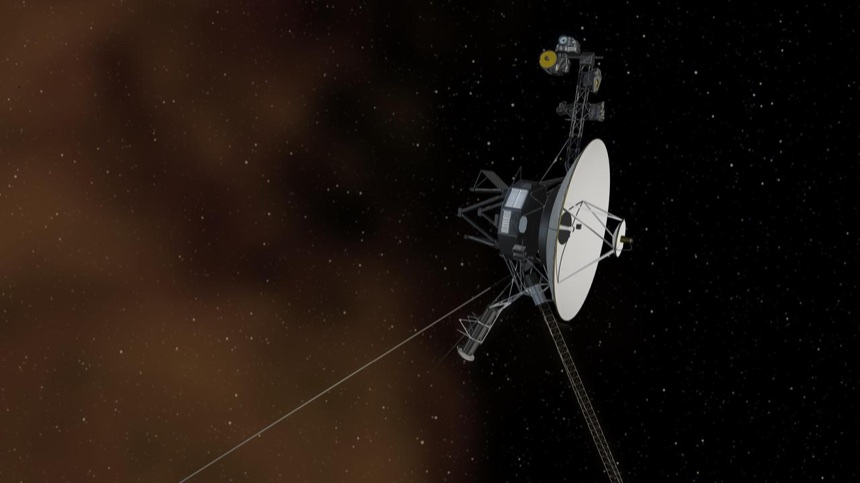
\includegraphics[width=0.78\textwidth,height=5.6cm,keepaspectratio]{../public/textures/nasa/voyager1.jpg}\\[3pt]
{\footnotesize\itshape\color{orbitarMuted} Randare oficială NASA/JPL-Caltech (PIA17462): Sonda Voyager 1 călătorind în spațiul interstelar cu Discul de Aur la bord.}
\end{center}


\begin{tcolorbox}[orbitardata, title={\textbf{Repere esențiale: Voyager 1}}]
\small
\begin{itemize}[leftmargin=1.4em, itemsep=2pt, topsep=2pt]
  \item \textbf{Clasificare și orbită:} Sondă Interplanetară \quad$\bullet$\quad \textbf{Distanță:} 165,000 UA ($\approx$ 24.684 milioane de kilometri)
  \item \textbf{Dimensiuni și masă:} anvergură de aproximativ 2 metri \quad$\bullet$\quad masă: Vehicul spațial artificial
  \item \textbf{Gravitație și regim termic:} Microgravitație / Imponderabilitate ($\approx 0\,g$) \quad$\bullet$\quad temperatură medie: -195 $^\circ$C
  \item \textbf{Ciclu orbital și rotație:} perioadă orbitală (an): 180.000 zile ($\approx$ 492,81 ani pământești) \quad$\bullet$\quad rotație (zi): 24,00 ore (1,00 zile pământești) (elemente kepleriene: $a = 42,500$ UA, $e = 0,2500$, $i = 35,70^\circ$, $\Omega = 178,0^\circ$, $\omega = 85,0^\circ$)
  \item \textbf{Durata călătoriei de pe Pământ:} cu viteza luminii ($1c$): \emph{22 de ore și 45 de minute}; cu racheta ($50.000$ de kilometri pe oră): \emph{47+ ani de zbor continuu (cu 61.000 kilometri pe oră)}; cu avionul ($900$ de kilometri pe oră): \emph{3.100 de ani}; cu mașina ($100$ de kilometri pe oră): \emph{28.000 de ani}.
  \item \textbf{Repere de scară și curiozitate:} Poartă cu ea un \guillemotleft{}Disc de Aur\guillemotright{} cu saluturi în 55 de limbi (inclusiv în limba română: \guillemotleft{}Salutări la toată lumea!\guillemotright{}), muzică și sunete de pe Pământ! Voyager 1 este atât de departe încât un mesaj radio care merge cu viteza luminii face aproape o zi întreagă până ajunge la ea!
\end{itemize}
\end{tcolorbox}

\vspace{4pt}
\noindent\textbf{Prezentare generală și profil astrofizic.} Lansată la 5 septembrie 1977, Voyager 1 a explorat sistemele lui Jupiter (1979) și Saturn (1980), iar la 25 august 2012 a traversat heliopauza, devenind primul artefact uman care pătrunde în mediul interstelar, la peste 24 de miliarde de kilometri de Pământ. Voyager 1 este cel mai curajos explorator construit vreodată de oameni! Zboară din anul 1977 și a ieșit deja din Sistemul Solar, în spațiul dintre stele. Poartă cu ea un \guillemotleft{}Disc de Aur\guillemotright{} cu saluturi în 55 de limbi (inclusiv în limba română: \guillemotleft{}Salutări la toată lumea!\guillemotright{}), muzică și sunete de pe Pământ!

\medskip
\noindent\textbf{Arhitectura tehnică și instrumentele științifice de la bord.} Din punct de vedere constructiv și ingineresc, vehiculul spațial reunește mai multe subsisteme și instrumente științifice de înaltă precizie, proiectate să funcționeze în condițiile extreme ale spațiului cosmic. În primul rând se remarcă \textbf{Antena parabolică de mare câștig (3,7 metri diametru)}, menținută permanent orientată către Pământ pentru comunicații prin rețeaua Deep Space Network. În strânsă legătură cu această componentă se află \textbf{Generatoare termoelectrice cu radioizotopi (3 $\times$ RTG)}, alimentate cu plutoniu-238, deoarece la distanțe mari lumina Soarelui este prea slabă pentru panouri solare. În completarea acestui ansamblu întâlnim \textbf{Discul de Aur (Voyager Golden Record) și Magnetometrele}, capsulă culturală a umanității și senzori care măsoară plasma și câmpul magnetic interstelar.

\medskip
\noindent\textbf{Observații astronomice și istoricul explorării.} A realizat în 1990 celebra fotografie a Pământului \guillemotleft{}Un punct albastru pal\guillemotright{} (Pale Blue Dot) de la 6 miliarde de kilometri distanță, la sugestia lui Carl Sagan. Voyager 1 este atât de departe încât un mesaj radio care merge cu viteza luminii face aproape o zi întreagă până ajunge la ea!

\vspace{6pt}
\begin{tcolorbox}[orbitarquiz, title={\textbf{Întrebare de verificare \#39: Voyager 1}}]
\textbf{Ce poartă la bord sondele Voyager 1 și Voyager 2 ca mesaj pentru eventuale civilizații extraterestre?}
\begin{itemize}[leftmargin=2.2em, itemsep=2pt, topsep=4pt]
  \item[$\square$ \textbf{A.}] Discul de Aur (Golden Record) cu sunete, imagini și saluturi în 55 de limbi, inclusiv în română
  \item[$\square$ \textbf{B.}] Un steag de hârtie
  \item[$\square$ \textbf{C.}] Un telescop cu oglindă de aur
  \item[$\square$ \textbf{D.}] Roci de pe Lună
\end{itemize}
\vspace{2pt}
{\footnotesize\color{orbitarMuted}\textbf{Răspuns corect:} \textbf{A} (Discul de Aur (Golden Record) cu sunete, imagini și saluturi în 55 de limbi, inclusiv în română). \emph{Discul de Aur Voyager conține 115 imagini, muzică de pe Pământ și saluturi în 55 de limbi (inclusiv \guillemotleft{}Salutări la toată lumea\guillemotright{} în limba română).}}
\end{tcolorbox}
\clearpage


\section{Voyager 2}
\label{sec:body-voyager2}
\vspace{-4pt}
{\large\itshape\color{orbitarAccent} Singura sondă din istorie care a vizitat toți cei 4 giganți: Jupiter, Saturn, Uranus și Neptun}\\[4pt]


\begin{center}
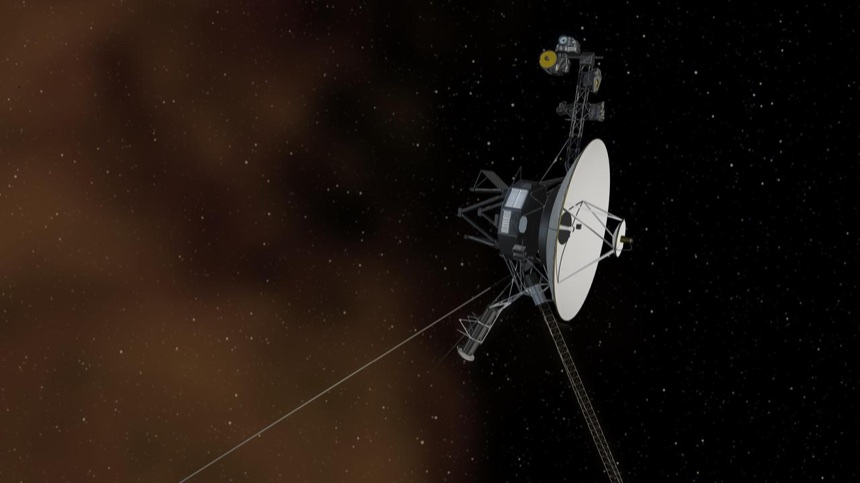
\includegraphics[width=0.78\textwidth,height=5.6cm,keepaspectratio]{../public/textures/nasa/voyager2.jpg}\\[3pt]
{\footnotesize\itshape\color{orbitarMuted} Randare oficială NASA/JPL-Caltech (PIA17462): Sonda Voyager 2, singura navă care a vizitat toți cei patru giganți planetari.}
\end{center}


\begin{tcolorbox}[orbitardata, title={\textbf{Repere esențiale: Voyager 2}}]
\small
\begin{itemize}[leftmargin=1.4em, itemsep=2pt, topsep=2pt]
  \item \textbf{Clasificare și orbită:} Sondă Interplanetară \quad$\bullet$\quad \textbf{Distanță:} 138,000 UA ($\approx$ 20.645 milioane de kilometri)
  \item \textbf{Dimensiuni și masă:} anvergură de aproximativ 2 metri \quad$\bullet$\quad masă: Vehicul spațial artificial
  \item \textbf{Gravitație și regim termic:} Microgravitație / Imponderabilitate ($\approx 0\,g$) \quad$\bullet$\quad temperatură medie: -195 $^\circ$C
  \item \textbf{Ciclu orbital și rotație:} perioadă orbitală (an): 165.000 zile ($\approx$ 451,75 ani pământești) \quad$\bullet$\quad rotație (zi): 24,00 ore (1,00 zile pământești) (elemente kepleriene: $a = 38,500$ UA, $e = 0,2200$, $i = -32,00^\circ$, $\Omega = 310,0^\circ$, $\omega = 45,0^\circ$)
  \item \textbf{Durata călătoriei de pe Pământ:} cu viteza luminii ($1c$): \emph{19 ore}; cu racheta ($50.000$ de kilometri pe oră): \emph{47+ ani}; cu avionul ($900$ de kilometri pe oră): \emph{2.600 de ani}; cu mașina ($100$ de kilometri pe oră): \emph{23.500 de ani}.
  \item \textbf{Repere de scară și curiozitate:} Folosind gravitația fiecărei planete ca pe o praștie cosmică, Voyager 2 a sărit de la o planetă la alta! Deși se numește Voyager 2, a fost lansată cu 16 zile ÎNAINTE de Voyager 1!
\end{itemize}
\end{tcolorbox}

\vspace{4pt}
\noindent\textbf{Prezentare generală și profil astrofizic.} Lansată la 20 august 1977, Voyager 2 a profitat de o aliniere planetară care apare doar o dată la 175 de ani (\guillemotleft{}Grand Tour\guillemotright{}), survolând Jupiter (1979), Saturn (1981), Uranus (1986) și Neptun (1989). În noiembrie 2018 a intrat și ea în spațiul interstelar. Voyager 2 este sora geamănă a lui Voyager 1 și singura navă spațială care a făcut \guillemotleft{}Marele Tur\guillemotright{}, vizitând toate cele patru planete uriașe: Jupiter, Saturn, Uranus și Neptun! Folosind gravitația fiecărei planete ca pe o praștie cosmică, Voyager 2 a sărit de la o planetă la alta!

\medskip
\noindent\textbf{Arhitectura tehnică și instrumentele științifice de la bord.} Din punct de vedere constructiv și ingineresc, vehiculul spațial reunește mai multe subsisteme și instrumente științifice de înaltă precizie, proiectate să funcționeze în condițiile extreme ale spațiului cosmic. În primul rând se remarcă \textbf{Antena parabolică de 3,7 metri și emițătorul în banda X}, prin care transmite date științifice cu o putere de doar aproximativ 20 W (cât un bec de frigider) de la peste 20 de miliarde de kilometri. În strânsă legătură cu această componentă se află \textbf{Sub-sistemul de analiză a plasmei (PLS)}, care a măsurat direct tranziția bruscă de la vântul solar cald la plasma interstelară rece. În completarea acestui ansamblu întâlnim \textbf{Platforma de scanare cu camere și spectrometre}, care a descoperit 16 sateliți noi, gheizerele de azot de pe Triton și inelele lui Uranus și Neptun.

\medskip
\noindent\textbf{Observații astronomice și istoricul explorării.} Rămâne până astăzi singura sondă care a explorat de aproape giganții de gheață Uranus și Neptun. Deși se numește Voyager 2, a fost lansată cu 16 zile ÎNAINTE de Voyager 1!

\vspace{6pt}
\begin{tcolorbox}[orbitarquiz, title={\textbf{Întrebare de verificare \#40: Voyager 2}}]
\textbf{Care este singura sondă spațială care a vizitat planetele Uranus și Neptun?}
\begin{itemize}[leftmargin=2.2em, itemsep=2pt, topsep=4pt]
  \item[$\square$ \textbf{A.}] Voyager 1
  \item[$\square$ \textbf{B.}] Voyager 2
  \item[$\square$ \textbf{C.}] Cassini
  \item[$\square$ \textbf{D.}] New Horizons
\end{itemize}
\vspace{2pt}
{\footnotesize\color{orbitarMuted}\textbf{Răspuns corect:} \textbf{B} (Voyager 2). \emph{Voyager 2 este singura navă spațială care a survolat toate cele patru planete gigante, inclusiv Uranus (1986) și Neptun (1989).}}
\end{tcolorbox}
\clearpage


\section{New Horizons}
\label{sec:body-newhorizons}
\vspace{-4pt}
{\large\itshape\color{orbitarAccent} Sonda rapidă care ne-a dezvăluit inima înghețată a lui Pluto și Centura Kuiper}\\[4pt]


\begin{center}
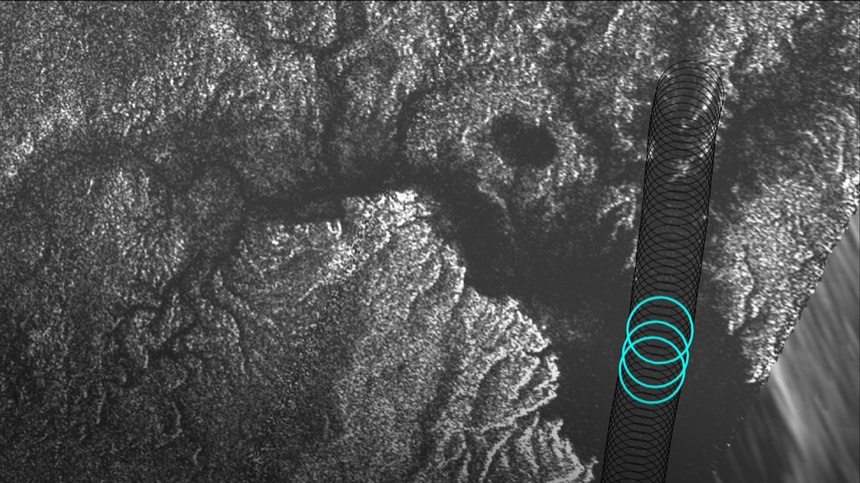
\includegraphics[width=0.78\textwidth,height=5.6cm,keepaspectratio]{../public/textures/nasa/newhorizons.jpg}\\[3pt]
{\footnotesize\itshape\color{orbitarMuted} Imagine oficială NASA/JHUAPL/SwRI: Sonda interplanetară New Horizons în timpul explorării Centurii Kuiper.}
\end{center}


\begin{tcolorbox}[orbitardata, title={\textbf{Repere esențiale: New Horizons}}]
\small
\begin{itemize}[leftmargin=1.4em, itemsep=2pt, topsep=2pt]
  \item \textbf{Clasificare și orbită:} Sondă Interplanetară \quad$\bullet$\quad \textbf{Distanță:} 60,200 UA ($\approx$ 9.006 milioane de kilometri)
  \item \textbf{Dimensiuni și masă:} anvergură de aproximativ 2,1 metri \quad$\bullet$\quad masă: Vehicul spațial artificial
  \item \textbf{Gravitație și regim termic:} Microgravitație / Imponderabilitate ($\approx 0\,g$) \quad$\bullet$\quad temperatură medie: -210 $^\circ$C
  \item \textbf{Ciclu orbital și rotație:} perioadă orbitală (an): 120.000 zile ($\approx$ 328,54 ani pământești) \quad$\bullet$\quad rotație (zi): 24,00 ore (1,00 zile pământești) (elemente kepleriene: $a = 35,000$ UA, $e = 0,2800$, $i = 14,50^\circ$, $\Omega = 115,0^\circ$, $\omega = 180,0^\circ$)
  \item \textbf{Durata călătoriei de pe Pământ:} cu viteza luminii ($1c$): \emph{8 ore și 20 de minute}; cu racheta ($50.000$ de kilometri pe oră): \emph{9,5 ani până la Pluto (18+ ani în Centura Kuiper)}; cu avionul ($900$ de kilometri pe oră): \emph{1.100 de ani}; cu mașina ($100$ de kilometri pe oră): \emph{10.000 de ani}.
  \item \textbf{Repere de scară și curiozitate:} A plecat de pe Pământ mai repede decât orice altă rachetă și a trecut de orbita Lunii în doar 9 ore (față de 3 zile cât le-a luat astronauților Apollo)! După Pluto, a vizitat în 2019 și pe Arrokoth, un corp înghețat din Centura Kuiper care arată exact ca un om de zăpadă cosmic!
\end{itemize}
\end{tcolorbox}

\vspace{4pt}
\noindent\textbf{Prezentare generală și profil astrofizic.} Lansată la 19 ianuarie 2006 cu cea mai mare viteză de evadare de pe Pământ (16,26 kilometri pe secundă), New Horizons a survolat Jupiter în 2007, sistemul Pluto--Charon la 14 iulie 2015 și obiectul primordial din Centura Kuiper 486958 Arrokoth la 1 ianuarie 2019. New Horizons este sonda spațială de mărimea unui pian cu coadă care a zburat timp de 9 ani și jumătate pentru a fotografia pentru prima oară de aproape planeta pitică Pluto! A plecat de pe Pământ mai repede decât orice altă rachetă și a trecut de orbita Lunii în doar 9 ore (față de 3 zile cât le-a luat astronauților Apollo)!

\medskip
\noindent\textbf{Arhitectura tehnică și instrumentele științifice de la bord.} Din punct de vedere constructiv și ingineresc, vehiculul spațial reunește mai multe subsisteme și instrumente științifice de înaltă precizie, proiectate să funcționeze în condițiile extreme ale spațiului cosmic. În primul rând se remarcă \textbf{Camera telescopică LORRI și spectrometrul Ralph}, care au cartografiat munții de gheață și câmpia Sputnik Planitia de pe Pluto la rezoluții de sub 100 de metri pe pixel. În strânsă legătură cu această componentă se află \textbf{Generator radioizotopic RTG și antenă de 2,1 metri}, care asigură energia și comunicațiile la peste 55--60 UA de Soare. În completarea acestui ansamblu întâlnim \textbf{Detectorul de praf Venetia Burney (SDC)}, construit de studenți și numit după fetița de 11 ani care a propus numele \guillemotleft{}Pluto\guillemotright{} în 1930.

\medskip
\noindent\textbf{Observații astronomice și istoricul explorării.} A realizat cel mai îndepărtat survol al unui corp ceresc din istorie (Arrokoth, la 43,4 UA de Soare). După Pluto, a vizitat în 2019 și pe Arrokoth, un corp înghețat din Centura Kuiper care arată exact ca un om de zăpadă cosmic!

\vspace{6pt}
\begin{tcolorbox}[orbitarquiz, title={\textbf{Întrebare de verificare \#41: New Horizons}}]
\textbf{În cât timp a ajuns sonda New Horizons de la Pământ până la orbita Lunii după lansarea din 2006?}
\begin{itemize}[leftmargin=2.2em, itemsep=2pt, topsep=4pt]
  \item[$\square$ \textbf{A.}] În 3 zile
  \item[$\square$ \textbf{B.}] În doar 9 ore
  \item[$\square$ \textbf{C.}] Într-o lună
  \item[$\square$ \textbf{D.}] Într-un an
\end{itemize}
\vspace{2pt}
{\footnotesize\color{orbitarMuted}\textbf{Răspuns corect:} \textbf{B} (În doar 9 ore). \emph{Lansată cu peste 58.000 kilometri pe oră, New Horizons a traversat distanța Pământ--Lună în doar 9 ore!}}
\end{tcolorbox}
\clearpage


\section{Parker Solar Probe}
\label{sec:body-parker}
\vspace{-4pt}
{\large\itshape\color{orbitarAccent} Sonda ultra-rapidă care a \guillemotleft{}atins\guillemotright{} Soarele, pătrunzând în coroana solară}\\[4pt]


\begin{center}
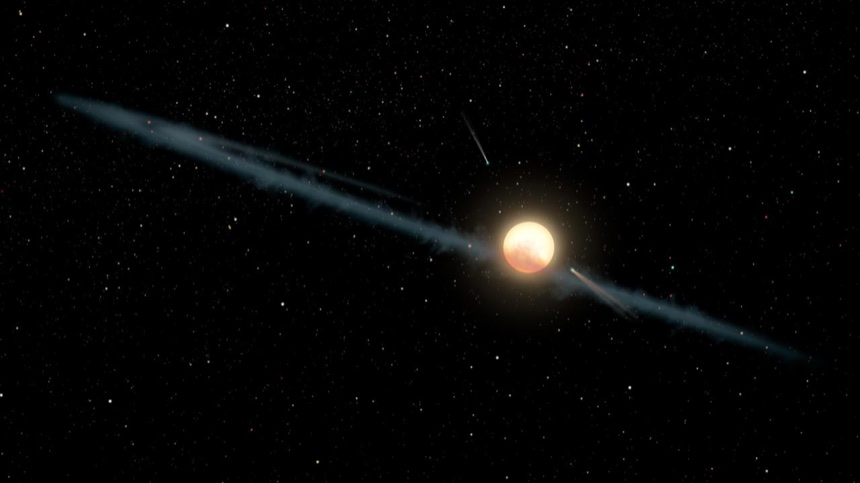
\includegraphics[width=0.78\textwidth,height=5.6cm,keepaspectratio]{../public/textures/nasa/parker.jpg}\\[3pt]
{\footnotesize\itshape\color{orbitarMuted} Imagine oficială NASA/JHUAPL: Sonda Parker Solar Probe zburând prin coroana solară incandescentă.}
\end{center}


\begin{tcolorbox}[orbitardata, title={\textbf{Repere esențiale: Parker Solar Probe}}]
\small
\begin{itemize}[leftmargin=1.4em, itemsep=2pt, topsep=2pt]
  \item \textbf{Clasificare și orbită:} Sondă Interplanetară \quad$\bullet$\quad \textbf{Distanță:} 0,250 UA ($\approx$ 37 milioane de kilometri)
  \item \textbf{Dimensiuni și masă:} anvergură de aproximativ 2 metri \quad$\bullet$\quad masă: Vehicul spațial artificial
  \item \textbf{Gravitație și regim termic:} Microgravitație / Imponderabilitate ($\approx 0\,g$) \quad$\bullet$\quad temperatură medie: +1.370 $^\circ$C
  \item \textbf{Ciclu orbital și rotație:} perioadă orbitală (an): 88 zile pământești \quad$\bullet$\quad rotație (zi): 24,00 ore (1,00 zile pământești) (elemente kepleriene: $a = 0,390$ UA, $e = 0,8800$, $i = 3,40^\circ$, $\Omega = 75,0^\circ$, $\omega = 15,0^\circ$)
  \item \textbf{Durata călătoriei de pe Pământ:} cu viteza luminii ($1c$): \emph{8 minute}; cu racheta ($50.000$ de kilometri pe oră): \emph{câteva luni}; cu avionul ($900$ de kilometri pe oră): \emph{18 ani}; cu mașina ($100$ de kilometri pe oră): \emph{160 de ani}.
  \item \textbf{Repere de scară și curiozitate:} Are în față un scut termic special, gros cât o carte, în spatele căruia instrumentele stau la o temperatură plăcută de cameră în timp ce afară sunt +1.400 $^\circ$C! Atinge viteza incredibilă de 690.000 de kilometri pe oră, viteză cu care ai ajunge de la București la Oradea în mai puțin de 3 secunde!
\end{itemize}
\end{tcolorbox}

\vspace{4pt}
\noindent\textbf{Prezentare generală și profil astrofizic.} Lansată în august 2018 și numită în onoarea astrofizicianului Eugene Parker (care a prezis existența vântului solar), sonda folosește 7 asistențe gravitaționale ale planetei Venus pentru a coborî periheliul până la aproximativ 6,1 milioane de kilometri de fotosfera solară. Parker Solar Probe este cea mai rapidă navă construită vreodată de oameni și singura care s-a apropiat atât de mult de Soare încât a zburat chiar prin atmosfera lui de foc! Are în față un scut termic special, gros cât o carte, în spatele căruia instrumentele stau la o temperatură plăcută de cameră în timp ce afară sunt +1.400 $^\circ$C!

\medskip
\noindent\textbf{Arhitectura tehnică și instrumentele științifice de la bord.} Din punct de vedere constructiv și ingineresc, vehiculul spațial reunește mai multe subsisteme și instrumente științifice de înaltă precizie, proiectate să funcționeze în condițiile extreme ale spațiului cosmic. În primul rând se remarcă \textbf{Scutul de protecție termică (Thermal Protection System)}, gros de 11,4 centimetri din compozit carbon-carbon și spumă de carbon, rezistă la temperaturi de 1.370 $^\circ$C. În strânsă legătură cu această componentă se află \textbf{Panouri solare răcite activ cu apă deionizată}, care se retrag în umbra scutului termic în timpul trecerilor apropiate pe lângă Soare. În completarea acestui ansamblu întâlnim \textbf{Instrumentele FIELDS, SWEAP, WISPR și IS$_\odot$IS}, care măsoară câmpurile magnetice, plasma coronală și fotografiaza structurile vântului solar.

\medskip
\noindent\textbf{Observații astronomice și istoricul explorării.} În 2021 a devenit prima navă care a traversat suprafața critică Alfvén, intrând oficial în atmosfera magnetică a Soarelui. Atinge viteza incredibilă de 690.000 de kilometri pe oră, viteză cu care ai ajunge de la București la Oradea în mai puțin de 3 secunde!

\vspace{6pt}
\begin{tcolorbox}[orbitarquiz, title={\textbf{Întrebare de verificare \#42: Parker Solar Probe}}]
\textbf{Ce record absolut deține sonda Parker Solar Probe?}
\begin{itemize}[leftmargin=2.2em, itemsep=2pt, topsep=4pt]
  \item[$\square$ \textbf{A.}] Cea mai grea rachetă
  \item[$\square$ \textbf{B.}] Cel mai rapid obiect construit vreodată de om (aproximativ 690.000 kilometri pe oră) și cel mai apropiat de Soare
  \item[$\square$ \textbf{C.}] Cea mai veche sondă
  \item[$\square$ \textbf{D.}] Singura sondă de pe Marte
\end{itemize}
\vspace{2pt}
{\footnotesize\color{orbitarMuted}\textbf{Răspuns corect:} \textbf{B} (Cel mai rapid obiect construit vreodată de om (aproximativ 690.000 kilometri pe oră) și cel mai apropiat de Soare). \emph{Atrăgând-o gravitația imensă a Soarelui la periheliu, Parker Solar Probe atinge aproximativ 191 kilometri pe secundă (690.000 kilometri pe oră).}}
\end{tcolorbox}
\clearpage


\section{Rosetta \& Philae}
\label{sec:body-rosetta}
\vspace{-4pt}
{\large\itshape\color{orbitarAccent} Misiunea europeană istorică ce a însoțit o cometă și a asolizat pe nucleul ei}\\[4pt]


\begin{center}
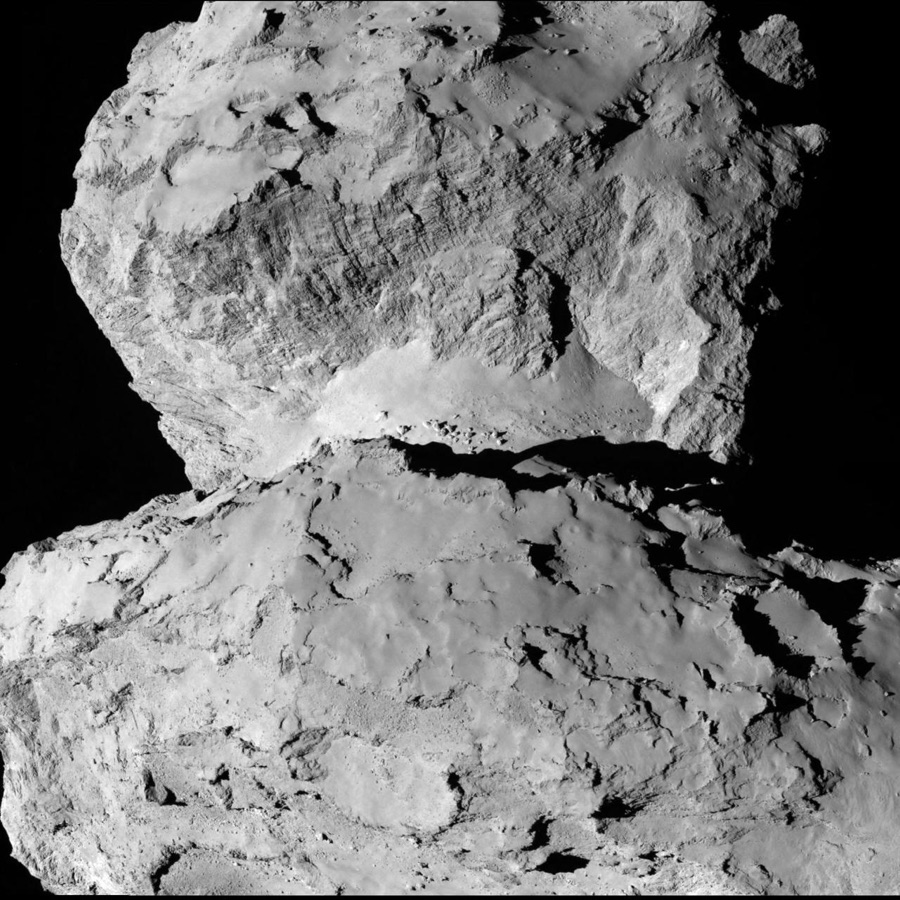
\includegraphics[width=0.78\textwidth,height=5.6cm,keepaspectratio]{../public/textures/nasa/rosetta.jpg}\\[3pt]
{\footnotesize\itshape\color{orbitarMuted} Fotografie oficială ESA/NASA (PIA18596): Nucleul bilobat al cometei 67P/Ciuriumov-Gherasimenko fotografiat de sonda Rosetta.}
\end{center}


\begin{tcolorbox}[orbitardata, title={\textbf{Repere esențiale: Rosetta \& Philae}}]
\small
\begin{itemize}[leftmargin=1.4em, itemsep=2pt, topsep=2pt]
  \item \textbf{Clasificare și orbită:} Sondă Interplanetară \quad$\bullet$\quad \textbf{Distanță:} 3,460 UA ($\approx$ 518 milioane de kilometri)
  \item \textbf{Dimensiuni și masă:} anvergură de aproximativ 2 metri \quad$\bullet$\quad masă: Vehicul spațial artificial
  \item \textbf{Gravitație și regim termic:} Microgravitație / Imponderabilitate ($\approx 0\,g$) \quad$\bullet$\quad temperatură medie: -70 $^\circ$C
  \item \textbf{Ciclu orbital și rotație:} perioadă orbitală (an): 2.352 zile ($\approx$ 6,44 ani pământești) \quad$\bullet$\quad rotație (zi): 12,40 ore (0,52 zile pământești) (elemente kepleriene: $a = 3,460$ UA, $e = 0,6400$, $i = 7,04^\circ$, $\Omega = 50,1^\circ$, $\omega = 12,8^\circ$)
  \item \textbf{Durata călătoriei de pe Pământ:} cu viteza luminii ($1c$): \emph{28 de minute}; cu racheta ($50.000$ de kilometri pe oră): \emph{10 ani (pe o traiectorie cu asistențe gravitaționale)}; cu avionul ($900$ de kilometri pe oră): \emph{50 de ani}; cu mașina ($100$ de kilometri pe oră): \emph{450 de ani}.
  \item \textbf{Repere de scară și curiozitate:} Cometa pe care a ajuns Rosetta are exact forma unei rățuște de baie din gheață și praf negru, lungă de 4 kilometri! Aripile solare ale sondei Rosetta erau lungi de 32 de metri, având lungimea unei balene albastre!
\end{itemize}
\end{tcolorbox}

\vspace{4pt}
\noindent\textbf{Prezentare generală și profil astrofizic.} Lansată de ESA în martie 2004, Rosetta a devenit în august 2014 prima sondă care a intrat pe orbita unei comete (67P/Ciuriumov-Gherasimenko), iar la 12 noiembrie 2014 modulul său Philae a realizat prima asolizare moale pe nucleul unei comete. Rosetta a fost sonda Agenției Spațiale Europene care a urmărit timp de 10 ani cometa Ciuriumov-Gherasimenko și a coborât pe ea micul robot laborator Philae! Cometa pe care a ajuns Rosetta are exact forma unei rățuște de baie din gheață și praf negru, lungă de 4 kilometri!

\medskip
\noindent\textbf{Arhitectura tehnică și instrumentele științifice de la bord.} Din punct de vedere constructiv și ingineresc, vehiculul spațial reunește mai multe subsisteme și instrumente științifice de înaltă precizie, proiectate să funcționeze în condițiile extreme ale spațiului cosmic. În primul rând se remarcă \textbf{Aripi solare de 64 metri pătrați cu celule LILT}, proiectate pentru intensitate luminoasă scăzută și temperaturi joase până la 5,2 UA de Soare. În strânsă legătură cu această componentă se află \textbf{Modulul de asolizare Philae (100 de kilograme)}, echipat cu harpoane, burghiu de eșantionare și 10 instrumente de analiză chimică și izotopică. În completarea acestui ansamblu întâlnim \textbf{Spectrometrul ROSINA și camera OSIRIS}, care au detectat aminoacidul glicină, fosfor și raportul deuteriu/hidrogen din apa cometară.

\medskip
\noindent\textbf{Observații astronomice și istoricul explorării.} Și-a încheiat misiunea la 30 septembrie 2016 coborând lent și așezându-se definitiv pe suprafața cometei 67P. Aripile solare ale sondei Rosetta erau lungi de 32 de metri, având lungimea unei balene albastre!

\vspace{6pt}
\begin{tcolorbox}[orbitarquiz, title={\textbf{Întrebare de verificare \#43: Rosetta \& Philae}}]
\textbf{Ce premieră mondială a realizat misiunea europeană Rosetta în anul 2014?}
\begin{itemize}[leftmargin=2.2em, itemsep=2pt, topsep=4pt]
  \item[$\square$ \textbf{A.}] A ajuns pe Pluto
  \item[$\square$ \textbf{B.}] A intrat pe orbita unei comete (67P) și a așezat robotul Philae pe suprafața ei
  \item[$\square$ \textbf{C.}] A adus roci de pe Marte
  \item[$\square$ \textbf{D.}] A fotografiat Soarele din interior
\end{itemize}
\vspace{2pt}
{\footnotesize\color{orbitarMuted}\textbf{Răspuns corect:} \textbf{B} (A intrat pe orbita unei comete (67P) și a așezat robotul Philae pe suprafața ei). \emph{Rosetta și modulul Philae au realizat prima orbitare și prima asolizare din istorie pe nucleul unei comete.}}
\end{tcolorbox}
\clearpage


\section{JUICE (Jupiter Icy Moons Explorer)}
\label{sec:body-juice}
\vspace{-4pt}
{\large\itshape\color{orbitarAccent} Exploratorul european al lunilor înghețate cu oceane ale lui Jupiter}\\[4pt]


\begin{center}
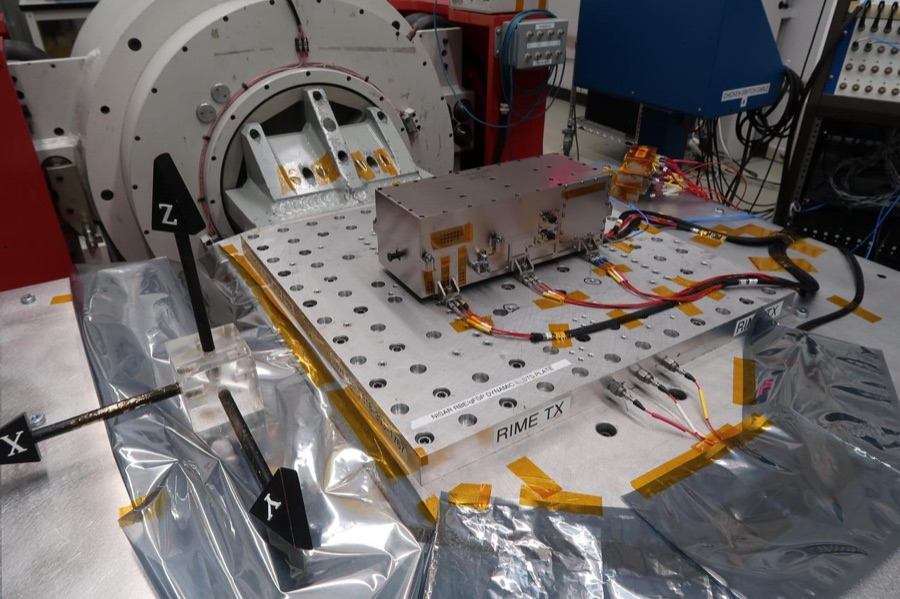
\includegraphics[width=0.78\textwidth,height=5.6cm,keepaspectratio]{../public/textures/nasa/juice.jpg}\\[3pt]
{\footnotesize\itshape\color{orbitarMuted} Fotografie oficială NASA/JPL/ESA (PIA24024): Sonda interplanetară europeană JUICE destinată studiului lunilor înghețate ale lui Jupiter.}
\end{center}


\begin{tcolorbox}[orbitardata, title={\textbf{Repere esențiale: JUICE (Jupiter Icy Moons Explorer)}}]
\small
\begin{itemize}[leftmargin=1.4em, itemsep=2pt, topsep=2pt]
  \item \textbf{Clasificare și orbită:} Sondă Interplanetară \quad$\bullet$\quad \textbf{Distanță:} 3,100 UA ($\approx$ 464 milioane de kilometri)
  \item \textbf{Dimensiuni și masă:} anvergură de aproximativ 2 metri \quad$\bullet$\quad masă: Vehicul spațial artificial
  \item \textbf{Gravitație și regim termic:} Microgravitație / Imponderabilitate ($\approx 0\,g$) \quad$\bullet$\quad temperatură medie: -150 $^\circ$C
  \item \textbf{Ciclu orbital și rotație:} perioadă orbitală (an): 1.850 zile ($\approx$ 5,07 ani pământești) \quad$\bullet$\quad rotație (zi): 24,00 ore (1,00 zile pământești) (elemente kepleriene: $a = 3,100$ UA, $e = 0,5200$, $i = 2,10^\circ$, $\Omega = 210,0^\circ$, $\omega = 60,0^\circ$)
  \item \textbf{Durata călătoriei de pe Pământ:} cu viteza luminii ($1c$): \emph{35 de minute}; cu racheta ($50.000$ de kilometri pe oră): \emph{8 ani (lansată în 2023, sosire la Jupiter în 2031)}; cu avionul ($900$ de kilometri pe oră): \emph{80 de ani}; cu mașina ($100$ de kilometri pe oră): \emph{717 ani}.
  \item \textbf{Repere de scară și curiozitate:} Cele două aripi solare ale sale, în formă de cruce, sunt mari cât un teren de baschet! Pe fuselajul sondei JUICE este gravat un desen realizat de o fetiță de 10 ani, ales dintr-un concurs la care au participat mii de copii!
\end{itemize}
\end{tcolorbox}

\vspace{4pt}
\noindent\textbf{Prezentare generală și profil astrofizic.} Lansată la 14 aprilie 2023 cu o rachetă Ariane 5, misiunea de clasă mare a ESA (JUICE) va ajunge în sistemul jovian în iulie 2031, va efectua 35 de survoluri ale lunilor Europa, Callisto și Ganymede, iar în 2034 va deveni prima sondă care orbitează o lună a altei planete (Ganymede). JUICE este sonda Agenției Spațiale Europene aflată în drum spre Jupiter pentru a cerceta oceanele ascunse sub gheață de pe lunile Europa, Callisto și Ganymede! Cele două aripi solare ale sale, în formă de cruce, sunt mari cât un teren de baschet!

\medskip
\noindent\textbf{Arhitectura tehnică și instrumentele științifice de la bord.} Din punct de vedere constructiv și ingineresc, vehiculul spațial reunește mai multe subsisteme și instrumente științifice de înaltă precizie, proiectate să funcționeze în condițiile extreme ale spațiului cosmic. În primul rând se remarcă \textbf{Panouri solare în formă de cruce (85 metri pătrați)}, cel mai mare sistem fotovoltaic trimis vreodată către Sistemul Solar exterior (unde lumina solară este de 25 de ori mai slabă). În strânsă legătură cu această componentă se află \textbf{Radarul de penetrare a gheții RIME (antena de 16 metri)}, care poate \guillemotleft{}vedea\guillemotright{} până la 9 kilometri adâncime prin crusta de gheață a lunilor joviane. În completarea acestui ansamblu întâlnim \textbf{Magnetometrul J-MAG și altimetrul laser GALA}, care vor măsura adâncimea și salinitatea oceanelor subterane de pe Ganymede, Europa și Callisto.

\medskip
\noindent\textbf{Observații astronomice și istoricul explorării.} În august 2024 a realizat prima manevră dublă din istorie de asistență gravitațională Lună--Pământ (LEGA). Pe fuselajul sondei JUICE este gravat un desen realizat de o fetiță de 10 ani, ales dintr-un concurs la care au participat mii de copii!

\vspace{6pt}
\begin{tcolorbox}[orbitarquiz, title={\textbf{Întrebare de verificare \#44: JUICE (Jupiter Icy Moons Explorer)}}]
\textbf{În jurul cărui satelit natural va intra pe orbită sonda europeană JUICE în anul 2034?}
\begin{itemize}[leftmargin=2.2em, itemsep=2pt, topsep=4pt]
  \item[$\square$ \textbf{A.}] Luna Pământului
  \item[$\square$ \textbf{B.}] Ganymede (cel mai mare satelit al lui Jupiter)
  \item[$\square$ \textbf{C.}] Titan
  \item[$\square$ \textbf{D.}] Io
\end{itemize}
\vspace{2pt}
{\footnotesize\color{orbitarMuted}\textbf{Răspuns corect:} \textbf{B} (Ganymede (cel mai mare satelit al lui Jupiter)). \emph{JUICE va deveni prima sondă din istorie care va intra pe orbită în jurul unui satelit al altei planete: Ganymede.}}
\end{tcolorbox}
\clearpage


\section{Perseverance \& Ingenuity}
\label{sec:body-perseverance}
\vspace{-4pt}
{\large\itshape\color{orbitarAccent} Laboratorul astrobiologic pe roți și primul elicopter care a zburat pe Marte}\\[4pt]


\begin{center}
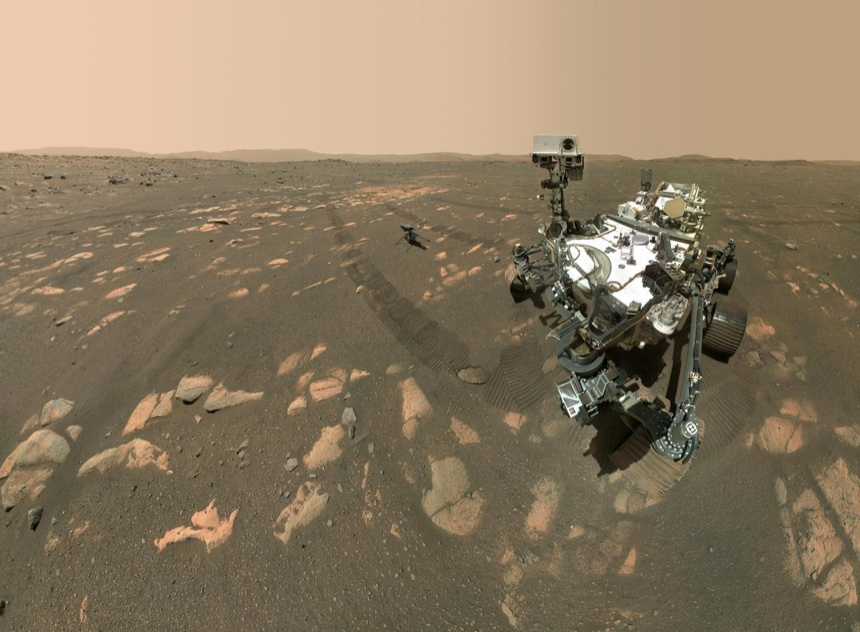
\includegraphics[width=0.78\textwidth,height=5.6cm,keepaspectratio]{../public/textures/nasa/perseverance.jpg}\\[3pt]
{\footnotesize\itshape\color{orbitarMuted} Fotografie reală NASA/JPL-Caltech (PIA24542): Roverul Perseverance alături de elicopterul Ingenuity în Craterul Jezero de pe Marte.}
\end{center}


\begin{tcolorbox}[orbitardata, title={\textbf{Repere esențiale: Perseverance \& Ingenuity}}]
\small
\begin{itemize}[leftmargin=1.4em, itemsep=2pt, topsep=2pt]
  \item \textbf{Clasificare și orbită:} Rover Planetar (orbitează în jurul: \textbf{Marte}) \quad$\bullet$\quad \textbf{Distanță:} 1,524 UA ($\approx$ 228 milioane de kilometri)
  \item \textbf{Dimensiuni și masă:} anvergură de aproximativ 2 metri \quad$\bullet$\quad masă: Vehicul spațial artificial
  \item \textbf{Gravitație și regim termic:} 0,380 $\times g_\oplus$ (3,73 m/s$^2$) \quad$\bullet$\quad temperatură medie: -63 $^\circ$C
  \item \textbf{Ciclu orbital și rotație:} perioadă orbitală (an): 686,98 zile ($\approx$ 1,88 ani pământești) \quad$\bullet$\quad rotație (zi): 24,62 ore (1,03 zile pământești)
  \item \textbf{Durata călătoriei de pe Pământ:} cu viteza luminii ($1c$): \emph{între 3 și 22 de minute}; cu racheta ($50.000$ de kilometri pe oră): \emph{7 luni (lansat în iulie 2020, amartizat în februarie 2021)}; cu avionul ($900$ de kilometri pe oră): \emph{7 ani}; cu mașina ($100$ de kilometri pe oră): \emph{62 de ani}.
  \item \textbf{Repere de scară și curiozitate:} Roverul este mare cât o mașină de teren, iar elicopterul Ingenuity cântărește doar 1,8 kilograme, cam cât o cutie mare de lapte! Ingenuity a fost primul aparat din istorie care a zburat pe o altă planetă, reușind 72 de zboruri în aerul subțire al lui Marte!
\end{itemize}
\end{tcolorbox}

\vspace{4pt}
\noindent\textbf{Prezentare generală și profil astrofizic.} Amartizat la 18 februarie 2021 în craterul Jezero (delta unui râu antic marțian), Perseverance caută biosemnături fosile, colectează carote de rocă în tuburi sigilate pentru viitoarea aducere pe Pământ și a demonstrat producerea de oxigen din atmosfera marțiană. Perseverance (\guillemotleft{}Percy\guillemotright{}) este un robot explorator pe 6 roți care caută urme de viață străveche în craterul Jezero de pe Marte, însoțit de micul elicopter Ingenuity (\guillemotleft{}Ginny\guillemotright{})! Roverul este mare cât o mașină de teren, iar elicopterul Ingenuity cântărește doar 1,8 kilograme, cam cât o cutie mare de lapte!

\medskip
\noindent\textbf{Arhitectura tehnică și instrumentele științifice de la bord.} Din punct de vedere constructiv și ingineresc, vehiculul spațial reunește mai multe subsisteme și instrumente științifice de înaltă precizie, proiectate să funcționeze în condițiile extreme ale spațiului cosmic. În primul rând se remarcă \textbf{Catargul cu SuperCam și Mastcam-Z}, camere panoramice cu zoom și un laser care vaporizează rocile de la 7 metri distanță pentru a le analiza compoziția. În strânsă legătură cu această componentă se află \textbf{Experimentul MOXIE}, care a produs cu succes oxigen respirabil direct din dioxidul de carbon (CO$_2$) al atmosferei marțiene. În completarea acestui ansamblu întâlnim \textbf{Elicopterul coaxial Ingenuity}, elice din fibră de carbon care se rotesc cu 2.400 rpm pentru a genera portanță în atmosfera marțiană cu densitate de doar 1\%.

\medskip
\noindent\textbf{Observații astronomice și istoricul explorării.} Coborât pe Marte prin spectaculoasa manevră \guillemotleft{}Sky Crane\guillemotright{} (macara zburătoare cu rachete); Ingenuity a zburat de 72 de ori între 2021 și 2024. Ingenuity a fost primul aparat din istorie care a zburat pe o altă planetă, reușind 72 de zboruri în aerul subțire al lui Marte!

\vspace{6pt}
\begin{tcolorbox}[orbitarquiz, title={\textbf{Întrebare de verificare \#45: Perseverance \& Ingenuity}}]
\textbf{Ce a demonstrat în premieră instrumentul MOXIE de la bordul roverului Perseverance?}
\begin{itemize}[leftmargin=2.2em, itemsep=2pt, topsep=4pt]
  \item[$\square$ \textbf{A.}] Că pe Marte plouă cu apă
  \item[$\square$ \textbf{B.}] Că se poate produce oxigen pur din atmosfera de dioxid de carbon a lui Marte
  \item[$\square$ \textbf{C.}] Că Marte are câmp magnetic puternic
  \item[$\square$ \textbf{D.}] Că există plante verzi
\end{itemize}
\vspace{2pt}
{\footnotesize\color{orbitarMuted}\textbf{Răspuns corect:} \textbf{B} (Că se poate produce oxigen pur din atmosfera de dioxid de carbon a lui Marte). \emph{MOXIE a extras oxigen din CO$_2$-ul atmosferic marțian, o tehnologie esențială pentru viitorii astronauți (pentru respirație și combustibil de rachetă).}}
\end{tcolorbox}
\clearpage


\section{Curiosity (Mars Science Laboratory)}
\label{sec:body-curiosity}
\vspace{-4pt}
{\large\itshape\color{orbitarAccent} Roverul veteran care urcă pe Muntele Sharp din craterul Gale de pe Marte}\\[4pt]


\begin{center}
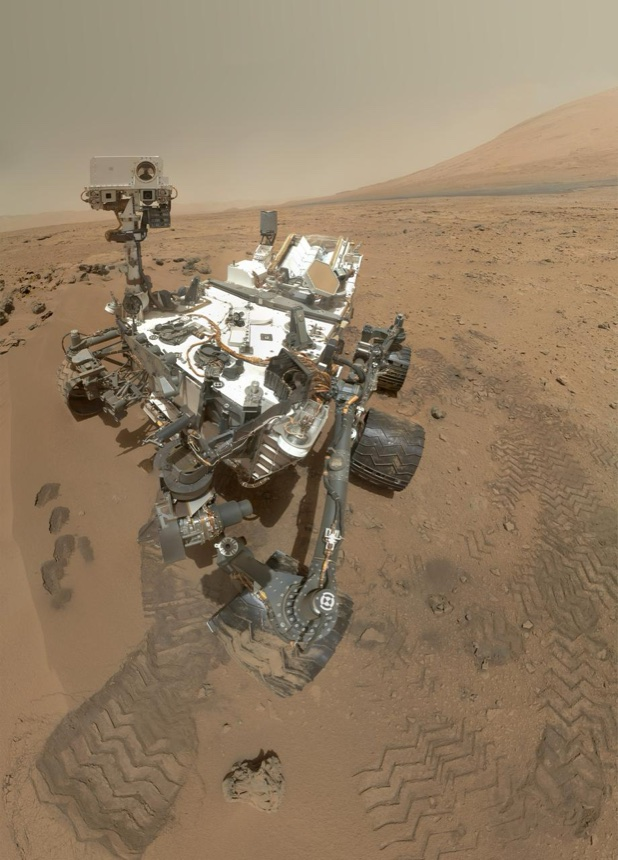
\includegraphics[width=0.78\textwidth,height=5.6cm,keepaspectratio]{../public/textures/nasa/curiosity.jpg}\\[3pt]
{\footnotesize\itshape\color{orbitarMuted} Autoportret real NASA/JPL-Caltech (PIA16239): Roverul Curiosity (MSL) pe solul Craterului Gale de pe Marte.}
\end{center}


\begin{tcolorbox}[orbitardata, title={\textbf{Repere esențiale: Curiosity (Mars Science Laboratory)}}]
\small
\begin{itemize}[leftmargin=1.4em, itemsep=2pt, topsep=2pt]
  \item \textbf{Clasificare și orbită:} Rover Planetar (orbitează în jurul: \textbf{Marte}) \quad$\bullet$\quad \textbf{Distanță:} 1,524 UA ($\approx$ 228 milioane de kilometri)
  \item \textbf{Dimensiuni și masă:} anvergură de aproximativ 2 metri \quad$\bullet$\quad masă: Vehicul spațial artificial
  \item \textbf{Gravitație și regim termic:} 0,380 $\times g_\oplus$ (3,73 m/s$^2$) \quad$\bullet$\quad temperatură medie: -63 $^\circ$C
  \item \textbf{Ciclu orbital și rotație:} perioadă orbitală (an): 686,98 zile ($\approx$ 1,88 ani pământești) \quad$\bullet$\quad rotație (zi): 24,62 ore (1,03 zile pământești)
  \item \textbf{Durata călătoriei de pe Pământ:} cu viteza luminii ($1c$): \emph{între 3 și 22 de minute}; cu racheta ($50.000$ de kilometri pe oră): \emph{8 luni și jumătate (2011--2012)}; cu avionul ($900$ de kilometri pe oră): \emph{7 ani}; cu mașina ($100$ de kilometri pe oră): \emph{62 de ani}.
  \item \textbf{Repere de scară și curiozitate:} Curiosity are un \guillemotleft{}cap\guillemotright{} cu 17 camere foto și un braț robotic lung de 2 metri cu care găurește pietrele marțiene! Roțile lui Curiosity au găuri speciale care lasă pe nisipul de pe Marte urme în codul Morse cu literele \guillemotleft{}J P L\guillemotright{} (laboratorul care l-a construit)!
\end{itemize}
\end{tcolorbox}

\vspace{4pt}
\noindent\textbf{Prezentare generală și profil astrofizic.} Amartizat la 6 august 2012 în craterul Gale, Curiosity (900 de kilograme, alimentat nuclear prin RTG) urcă treptat pe versanții muntelui Aeolis Mons (Mount Sharp, 5,5 kilometri înălțime), citind în straturile sedimentare tranziția lui Marte de la o lume umedă la un deșert rece. Curiosity este laboratorul chimic pe roți care explorează Marte încă din anul 2012! El a demonstrat că pe Marte au existat lacuri cu apă dulce în care ar fi putut trăi microbi. Curiosity are un \guillemotleft{}cap\guillemotright{} cu 17 camere foto și un braț robotic lung de 2 metri cu care găurește pietrele marțiene!

\medskip
\noindent\textbf{Arhitectura tehnică și instrumentele științifice de la bord.} Din punct de vedere constructiv și ingineresc, vehiculul spațial reunește mai multe subsisteme și instrumente științifice de înaltă precizie, proiectate să funcționeze în condițiile extreme ale spațiului cosmic. În primul rând se remarcă \textbf{Laboratorul intern SAM (Sample Analysis at Mars)}, spectrometru de masă și cromatograf cu gaz care a identificat molecule organice complexe în argilele marțiene. În strânsă legătură cu această componentă se află \textbf{Instrumentul cu laser ChemCam și difractometrul CheMin}, care identifică mineralele formate în prezența apei cu pH neutru. În completarea acestui ansamblu întâlnim \textbf{Suspensia Rocker-Bogie cu 6 roți motoare}, care permite roverului să treacă peste obstacole de două ori mai mari decât diametrul roților fără să se răstoarne.

\medskip
\noindent\textbf{Observații astronomice și istoricul explorării.} A parcurs peste 32 de kilometri pe Marte în mai mult de 4.300 de zile marțiene (soli), fiind încă activ. Roțile lui Curiosity au găuri speciale care lasă pe nisipul de pe Marte urme în codul Morse cu literele \guillemotleft{}J P L\guillemotright{} (laboratorul care l-a construit)!

\vspace{6pt}
\begin{tcolorbox}[orbitarquiz, title={\textbf{Întrebare de verificare \#46: Curiosity (Mars Science Laboratory)}}]
\textbf{Ce descoperire fundamentală a făcut roverul Curiosity în craterul Gale de pe Marte?}
\begin{itemize}[leftmargin=2.2em, itemsep=2pt, topsep=4pt]
  \item[$\square$ \textbf{A.}] Că Marte nu a avut niciodată apă
  \item[$\square$ \textbf{B.}] Că în trecutul îndepărtat al lui Marte au existat lacuri și râuri de apă lichidă cu condiții prielnice vieții microbiene
  \item[$\square$ \textbf{C.}] Că solul este din aur pur
  \item[$\square$ \textbf{D.}] Că Marte are inele
\end{itemize}
\vspace{2pt}
{\footnotesize\color{orbitarMuted}\textbf{Răspuns corect:} \textbf{B} (Că în trecutul îndepărtat al lui Marte au existat lacuri și râuri de apă lichidă cu condiții prielnice vieții microbiene). \emph{Analizând pietrișul rotunjit de apă și argilele din craterul Gale, Curiosity a demonstrat că Marte a găzduit lacuri străvechi de apă potabilă.}}
\end{tcolorbox}
\clearpage


% SPDX-License-Identifier: GPL-3.0-or-later
\chapter{Dincolo de Soare: Stele Apropiate și Exoplanete}
\label{chap:exoplanete}

Când comutăm în \textbf{Orbitar} de la \emph{Orizontul 1 (Sistemul Solar)} la \textbf{Orizontul 2 („Stele și Exoplanete”)}, părăsim căldura Soarelui nostru și pășim în \textbf{vecinătatea stelară}, unde distanțele nu se mai măsoară în kilometri sau Unități Astronomice, ci în \textbf{ani-lumină} ($1\text{ an-lumină}$ reprezintă aproximativ $9.460$ de miliarde de kilometri). În centrul scenei 3D rămâne aprins farul interactiv \textbf{„Aici este Sistemul nostru Solar (Acasă)”}, înconjurat de cele mai fascinante sisteme stelare și exoplanetare din jurul nostru.

\section*{Ce este o Exoplanetă și cum le descoperă astronomii?}

O \textbf{exoplanetă} (sau planetă extrasolară) este o planetă care orbitează în jurul altei stele decât Soarele nostru. Prima exoplanetă în jurul unei stele asemănătoare Soarelui (\emph{51 Pegasi b}) a fost descoperită în anul \textbf{1995} de astronomii elvețieni Michel Mayor și Didier Queloz (Premiul Nobel pentru Fizică). De atunci, telescoapele spațiale \emph{Kepler}, \emph{Spitzer}, \emph{TESS} și \emph{James Webb} au confirmat peste \textbf{5.700 de exoplanete} în Calea Lactee!

\begin{tcolorbox}[orbitardata, title={\textbf{Cum găsim o planetă ascunsă în strălucirea unei stele îndepărtate?}}]
Deoarece stelele sunt de milioane sau miliarde de ori mai strălucitoare decât planetele lor, astronomii folosesc metode ingenioase pentru a detecta exoplanetele:
\begin{enumerate}[leftmargin=1.5em, itemsep=3pt]
  \item \textbf{Metoda Tranzitului (Eclipsa în miniatură):} atunci când o exoplanetă trece exact prin fața stelei sale (privită dinspre Pământ), ea blochează o mică fracțiune din lumina stelei (de obicei între $0{,}01\%$ și $1\%$). Măsurând această scădere periodică de strălucire, aflăm raza exactă a planetei și durata anului ei! Mai mult, \textbf{Telescopul Spațial James Webb} analizează lumina stelară filtrată prin atmosfera exoplanetei în timpul tranzitului (spectroscopie de transmisie) pentru a detecta vapori de apă, dioxid de carbon sau metan.
  \item \textbf{Metoda Vitezei Radiale (Efectul Doppler):} planeta și steaua se atrag reciproc și se rotesc în jurul centrului comun de masă. Acest „dans” face ca steaua să oscileze ușor înainte și înapoi față de noi, deplasându-i spectrul luminos spre albastru și spre roșu. Din această oscilație calculăm \textbf{masa} exoplanetei!
  \item \textbf{Zona Locuibilă („Zona Goldilocks”):} este regiunea din jurul unei stele unde nu este nici prea cald (ca apa să fiarbă și să se evapore), nici prea frig (ca apa să înghețe complet), permițând existența \textbf{apei lichide} la suprafața unei planete stâncoase, așa cum se întâmplă pe \textbf{Proxima Centauri b} și pe planetele \textbf{TRAPPIST-1d, e și f}!
\end{enumerate}
\end{tcolorbox}

\begin{center}
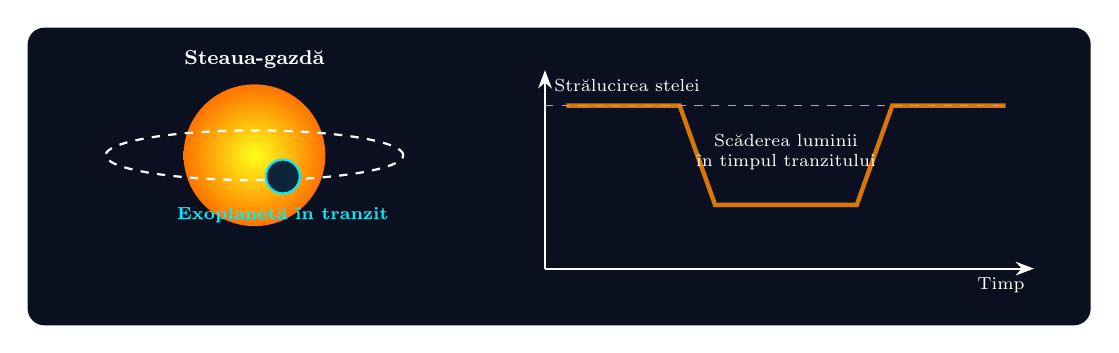
\begin{tikzpicture}[scale=0.90, every node/.style={transform shape}]
  \fill[orbitarSpaceBg, rounded corners=6pt] (-0.8,-2.1) rectangle (14.2,2.1);

  % Steaua gazdă
  \shade[inner color=yellow!90!white, outer color=orange!90!red] (2.4,0.3) circle (1.0cm);
  \node[white, font=\footnotesize\bfseries] at (2.4,1.65) {Steaua-gazdă};

  % Orbita exoplanetei
  \draw[white!40, dashed, line width=0.8pt] (2.4,0.3) ellipse (2.1cm and 0.35cm);
  % Exoplaneta în tranzit
  \fill[orbitarDeepBlue!90!black, draw=orbitarCyan, line width=0.8pt] (2.8,0.0) circle (0.24cm);
  \node[orbitarCyan, font=\scriptsize\bfseries] at (2.8,-0.55) {Exoplanetă în tranzit};

  % Graficul curbei de lumină în dreapta
  \draw[-{Stealth}, white!80, line width=0.8pt] (6.5,-1.3) -- (13.4,-1.3) node[below left, font=\scriptsize, text=white] {Timp};
  \draw[-{Stealth}, white!80, line width=0.8pt] (6.5,-1.3) -- (6.5,1.5) node[below right, font=\scriptsize, text=white] {Strălucirea stelei};

  % Curba de lumină
  \draw[orbitarAmber, line width=1.6pt] (6.8,1.0) -- (8.4,1.0) -- (8.9,-0.4) -- (10.9,-0.4) -- (11.4,1.0) -- (13.0,1.0);
  \draw[orbitarCyan, dashed] (6.5,1.0) -- (13.0,1.0);
  \node[white!90, font=\scriptsize, align=center] at (9.9,0.35) {Scăderea luminii\\în timpul tranzitului};
\end{tikzpicture}
\end{center}

\begin{table}[H]
\centering
\small
\caption{Cele 7 sisteme și corpuri din Orizontul 2 („Stele și Exoplanete”) în Orbitar}
\resizebox{\textwidth}{!}{%
\begin{tabular}{@{}lllr@{}}
\toprule
\textbf{Nume Sistem / Obiect} & \textbf{Categorie} & \textbf{Distanță față de Soare} & \textbf{Temp. caracteristică} \\
\midrule
Norul lui Oort & Rezervor Cometar Circumsolar & $\sim$1 an-lumină (63.241 UA) & -269$^\circ$C \\
Proxima Centauri \& Proxima b & Sistem Exoplanetar / Exoplanetă & 4,24 ani-lumină & -39$^\circ$C \\
Sirius A \& B (Luceafărul Câinelui) & Stea & 8,6 ani-lumină & 9.667$^\circ$C \\
Sistemul TRAPPIST-1 (7 Exoplanete) & Sistem Exoplanetar / Exoplanetă & 40 de ani-lumină & -22$^\circ$C \\
Exoplaneta 55 Cancri e (Janssen) & Sistem Exoplanetar / Exoplanetă & 41 de ani-lumină & 2.000$^\circ$C \\
Roiul Stelar Pleiadele (\quotedblbase{}Cloșca cu Pui\textquotedblright{}) & Roi Stelar Deschis & 444 de ani-lumină & 12.000$^\circ$C \\
Betelgeuse (Supergiganta Roșie) & Stea & 640 de ani-lumină & 3.327$^\circ$C \\
\bottomrule
\end{tabular}%
}
\end{table}

\clearpage

\section{Norul lui Oort}
\label{sec:body-oort_cloud}
\vspace{-4pt}
{\large\itshape\color{orbitarAccent} Sfera uriașă de comete înghețate de la granița Sistemului Solar (aproximativ 1 an-lumină)}\\[4pt]


\begin{center}
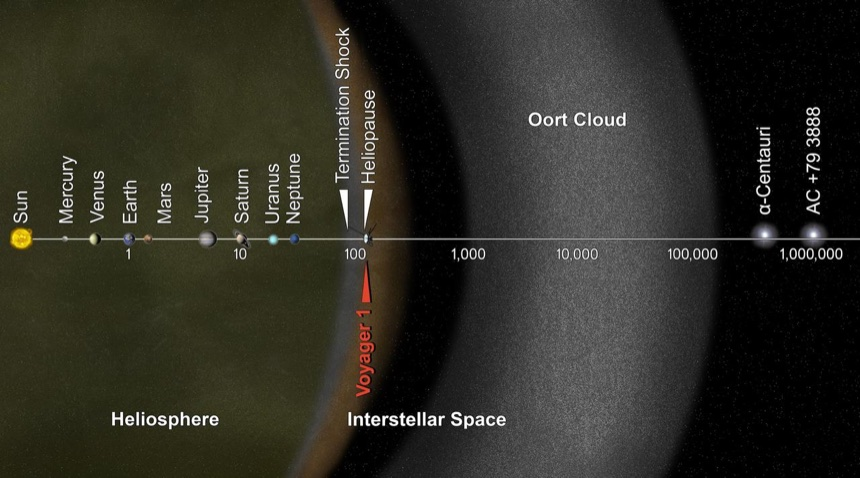
\includegraphics[width=0.78\textwidth,height=5.6cm,keepaspectratio]{../public/textures/nasa/oort_cloud.jpg}\\[3pt]
{\footnotesize\itshape\color{orbitarMuted} Ilustrație științifică oficială NASA/JPL-Caltech (PIA17046): Sfera gigantică de comete înghețate a Norului lui Oort în jurul Sistemului Solar.}
\end{center}


\begin{tcolorbox}[orbitardata, title={\textbf{Repere esențiale: Norul lui Oort}}]
\small
\begin{itemize}[leftmargin=1.4em, itemsep=2pt, topsep=2pt]
  \item \textbf{Clasificare și orbită:} Rezervor Cometar Circumsolar \quad$\bullet$\quad \textbf{Distanță:} aproximativ 1 an-lumină (63.241 UA)
  \item \textbf{Dimensiuni și masă:} Înconjoară întregul Sistem Solar ca o bulă sferică de aproximativ 100.000 de ori mai departe de Soare decât Pământul! \quad$\bullet$\quad masă: 5,000 $\times M_\oplus$
  \item \textbf{Gravitație și regim termic:} Microgravitație / Imponderabilitate ($\approx 0\,g$) \quad$\bullet$\quad temperatură medie: -269 $^\circ$C
  \item \textbf{Ciclu orbital și rotație:} perioadă orbitală (an): 365.250.000 zile ($\approx$ 1000000,00 ani pământești) \quad$\bullet$\quad rotație (zi): 24,00 ore (1,00 zile pământești)
  \item \textbf{Durata călătoriei de pe Pământ:} cu viteza luminii ($1c$): \emph{1 an}; cu racheta ($50.000$ de kilometri pe oră): \emph{21.600 de ani}; cu avionul ($900$ de kilometri pe oră): \emph{1,2 miliarde de ani}; cu mașina ($100$ de kilometri pe oră): \emph{10,8 miliarde de ani}.
  \item \textbf{Repere de scară și curiozitate:} Dacă Pământul ar fi la doar un pas de Soare, Norul lui Oort ar fi un balon uriaș de fulgi de zăpadă aflat la peste 50 de kilometri depărtare! Sondei Voyager 1 îi vor trebui încă 300 de ani doar ca să ajungă la marginea interioară a Norului lui Oort și aproximativ 30.000 de ani ca să îl traverseze complet!
\end{itemize}
\end{tcolorbox}

\vspace{4pt}
\noindent\textbf{Prezentare generală și profil astrofizic.} Norul lui Oort este un rezervor sferic imens de corpuri înghețate (apă, metan, amoniac și monoxid de carbon înghețat), situat între 2.000 și 100.000 UA (aproximativ 1 an-lumină) de Soare. El marchează limita sferei Hill a Sistemului Solar, adică frontiera până la care gravitația Soarelui mai poate reține obiecte pe orbită. La marginea cea mai îndepărtată a Sistemului nostru Solar, acolo unde căldura Soarelui abia se mai simte, plutește o bulă gigantică formată din miliarde de bulgări de gheață și praf cosmic. Acesta este Norul lui Oort, regiunea îndepărtată din care pornesc spre noi cometele cu coadă lungă și strălucitoare! Dacă Pământul ar fi la doar un pas de Soare, Norul lui Oort ar fi un balon uriaș de fulgi de zăpadă aflat la peste 50 de kilometri depărtare!

\medskip
\noindent\textbf{Scara cosmică și călătoria luminii în timp.} La scară astronomică, dimensiunile sale sunt impresionante: Înconjoară întregul Sistem Solar ca o bulă sferică de aproximativ 100.000 de ori mai departe de Soare decât Pământul! Totodată, privind astăzi spre Norul lui Oort, observăm practic trecutul îndepărtat al Universului, întrucât lumina sa a călătorit prin spațiu până la noi: Lumina de la marginea Norului lui Oort călătorește un an întreg până ajunge la ochii noștri pe Pământ!

\medskip
\noindent\textbf{Alcătuirea fizică și structura internă.} Privind în profunzimea sa, alcătuirea fizică este organizată pe mai multe straturi și regiuni distincte, fiecare având un rol bine definit în evoluția și dinamica acestui obiect cosmic. În primul rând se remarcă \textbf{Discul Interior (Norul Hills)}, regiune în formă de tor (2.000 -- 20.000 UA) care alimentează continuu norul exterior cu nuclee cometare. În completarea acestui ansamblu întâlnim \textbf{Sfera Exterioară Oort}, înveliș sferic (20.000 -- 100.000 UA) conținând miliarde de nuclee de comete de perioadă lungă, ușor perturbate de stelele vecine.

\medskip
\noindent\textbf{Observații astronomice și istoricul explorării.} Prezis teoretic de astronomul estonian Ernst Öpik (1932) și de astronomul olandez Jan Oort (1950) pentru a explica de unde vin cometele cu perioade de mii sau milioane de ani. Sondei Voyager 1 îi vor trebui încă 300 de ani doar ca să ajungă la marginea interioară a Norului lui Oort și aproximativ 30.000 de ani ca să îl traverseze complet!

\vspace{6pt}
\begin{tcolorbox}[orbitarquiz, title={\textbf{Întrebare de verificare \#47: Norul lui Oort}}]
\textbf{Ce se găsește în principal în Norul lui Oort, la aproximativ 1 an-lumină de Soare?}
\begin{itemize}[leftmargin=2.2em, itemsep=2pt, topsep=4pt]
  \item[$\square$ \textbf{A.}] Miliarde de nuclee înghețate de comete la granița Sistemului Solar
  \item[$\square$ \textbf{B.}] Planete gazoase fierbinți
  \item[$\square$ \textbf{C.}] Rovere marțiene
  \item[$\square$ \textbf{D.}] Doar sateliți artificiali
\end{itemize}
\vspace{2pt}
{\footnotesize\color{orbitarMuted}\textbf{Răspuns corect:} \textbf{A} (Miliarde de nuclee înghețate de comete la granița Sistemului Solar). \emph{Norul lui Oort este rezervorul sferic uriaș de comete înghețate aflat la limita atracției gravitaționale a Soarelui (aproximativ 1 an-lumină).}}
\end{tcolorbox}
\clearpage


\section{Proxima Centauri \& Proxima b}
\label{sec:body-proxima_centauri}
\vspace{-4pt}
{\large\itshape\color{orbitarAccent} Cea mai apropiată stea de Soare și exoplaneta ei stâncoasă (4,24 ani-lumină)}\\[4pt]


\begin{center}
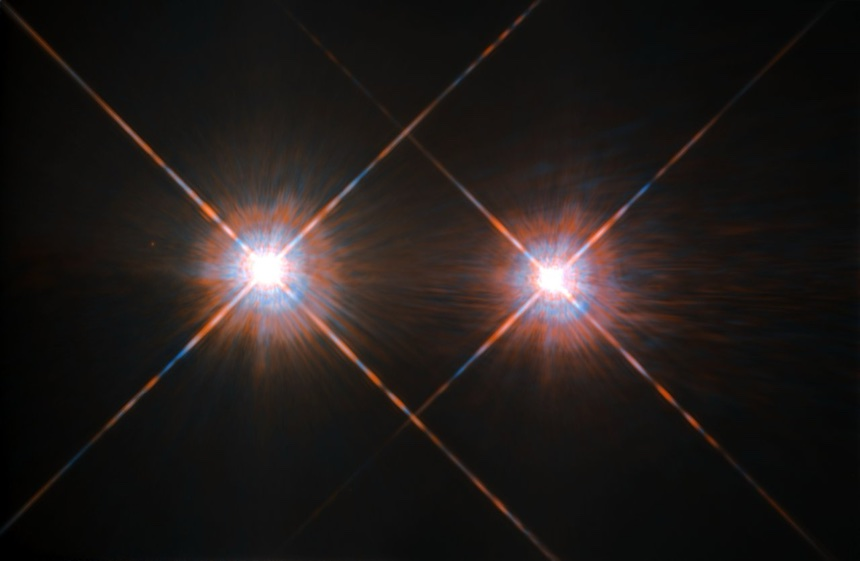
\includegraphics[width=0.78\textwidth,height=5.6cm,keepaspectratio]{../public/textures/nasa/proxima_centauri.jpg}\\[3pt]
{\footnotesize\itshape\color{orbitarMuted} Fotografie reală NASA/ESA (Telescopul Spațial Hubble WFPC2): Steaua pitică roșie Proxima Centauri, aflată la 4,24 ani-lumină.}
\end{center}


\begin{tcolorbox}[orbitardata, title={\textbf{Repere esențiale: Proxima Centauri \& Proxima b}}]
\small
\begin{itemize}[leftmargin=1.4em, itemsep=2pt, topsep=2pt]
  \item \textbf{Clasificare și orbită:} Sistem Exoplanetar / Exoplanetă \quad$\bullet$\quad \textbf{Distanță:} 4,24 ani-lumină
  \item \textbf{Dimensiuni și masă:} Steaua Proxima Centauri are doar 15\% din diametrul Soarelui (cât 1,5 planete Jupiter), iar exoplaneta Proxima b este puțin mai mare decât Pământul (1,07 raze terestre)! \quad$\bullet$\quad masă: 40900,000 $\times M_\oplus$
  \item \textbf{Gravitație și regim termic:} 1,100 $\times g_\oplus$ (10,79 m/s$^2$) \quad$\bullet$\quad temperatură medie: -39 $^\circ$C
  \item \textbf{Ciclu orbital și rotație:} perioadă orbitală (an): 11,186 zile pământești \quad$\bullet$\quad rotație (zi): 268,40 ore (11,18 zile pământești)
  \item \textbf{Durata călătoriei de pe Pământ:} cu viteza luminii ($1c$): \emph{4 ani și 3 luni}; cu racheta ($50.000$ de kilometri pe oră): \emph{75.000 de ani}; cu avionul ($900$ de kilometri pe oră): \emph{5,3 miliarde de ani}; cu mașina ($100$ de kilometri pe oră): \emph{48 de miliarde de ani}.
  \item \textbf{Repere de scară și curiozitate:} Dacă Soarele ar fi un pepene mare și galben, Proxima Centauri ar fi o cireașă roșie strălucitoare, iar planeta Proxima b o bobiță de mazăre care face un tur complet în jurul ei în doar 11 zile! Pe planeta Proxima b, un an întreg durează doar 11 zile pământești! Acolo ai sărbători ziua ta de naștere de trei ori pe lună!
\end{itemize}
\end{tcolorbox}

\vspace{4pt}
\noindent\textbf{Prezentare generală și profil astrofizic.} Situată la 4,24 ani-lumină în constelația Centaurul (parte a sistemului triplu Alpha Centauri), Proxima Centauri este o pitică roșie de clasă spectrală M5.5Ve. Exoplaneta Proxima Centauri b (descoperită în 2016) orbitează chiar în zona locuibilă (la 0,0485 UA de stea), unde temperatura ar permite existența apei lichide. Proxima Centauri este prima noastră vecină stelară din Univers! Este o stea pitică roșie, mai mică și mai blândă decât Soarele, iar în jurul ei se învârte Proxima Centauri b, care este cea mai apropiată exoplanetă (planetă din afara Sistemului Solar) de Pământ! Dacă Soarele ar fi un pepene mare și galben, Proxima Centauri ar fi o cireașă roșie strălucitoare, iar planeta Proxima b o bobiță de mazăre care face un tur complet în jurul ei în doar 11 zile!

\medskip
\noindent\textbf{Scara cosmică și călătoria luminii în timp.} La scară astronomică, dimensiunile sale sunt impresionante: Steaua Proxima Centauri are doar 15\% din diametrul Soarelui (cât 1,5 planete Jupiter), iar exoplaneta Proxima b este puțin mai mare decât Pământul (1,07 raze terestre)! Totodată, privind astăzi spre Proxima Centauri \& Proxima b, observăm practic trecutul îndepărtat al Universului, întrucât lumina sa a călătorit prin spațiu până la noi: Lumina de la Proxima Centauri pe care o vedem azi a plecat acum mai bine de 4 ani și 3 luni, pe când erai cu patru ani mai mic!

\medskip
\noindent\textbf{Alcătuirea fizică și structura internă.} Privind în profunzimea sa, alcătuirea fizică este organizată pe mai multe straturi și regiuni distincte, fiecare având un rol bine definit în evoluția și dinamica acestui obiect cosmic. În primul rând se remarcă \textbf{Steaua Proxima Centauri (M5.5V)}, pitică roșie cu temperatura la suprafață de aproximativ 3.042 K și o durată de viață de mii de miliarde de ani. În strânsă legătură cu această componentă se află \textbf{Exoplaneta Proxima Centauri b}, planetă telurică cu masa minimă de 1,17 mase terestre, orbitând în 11,2 zile în zona locuibilă a stelei. În completarea acestui ansamblu întâlnim \textbf{Proxima Centauri d}, un sub-Pământ foarte apropiat de stea (perioadă orbitală de doar 5,1 zile), descoperit în 2022.

\medskip
\noindent\textbf{Observații astronomice și istoricul explorării.} Steaua a fost descoperită în 1915 de Robert Innes, iar exoplaneta Proxima b a fost confirmată în august 2016 de Observatorul European Austral (ESO) prin metoda vitezelor radiale (instrumentul HARPS). Pe planeta Proxima b, un an întreg durează doar 11 zile pământești! Acolo ai sărbători ziua ta de naștere de trei ori pe lună!

\vspace{6pt}
\begin{tcolorbox}[orbitarquiz, title={\textbf{Întrebare de verificare \#48: Proxima Centauri \& Proxima b}}]
\textbf{La ce distanță de noi se află Proxima Centauri, cea mai apropiată stea de Sistemul Solar?}
\begin{itemize}[leftmargin=2.2em, itemsep=2pt, topsep=4pt]
  \item[$\square$ \textbf{A.}] 4,24 ani-lumină
  \item[$\square$ \textbf{B.}] 100 de kilometri
  \item[$\square$ \textbf{C.}] 2,5 milioane de ani-lumină
  \item[$\square$ \textbf{D.}] 1 Unitate Astronomică
\end{itemize}
\vspace{2pt}
{\footnotesize\color{orbitarMuted}\textbf{Răspuns corect:} \textbf{A} (4,24 ani-lumină). \emph{Proxima Centauri se află la 4,24 ani-lumină (aproximativ 40.000 de miliarde de kilometri) de Sistemul nostru Solar.}}
\end{tcolorbox}
\clearpage


\section{Sirius A \& B (Luceafărul Câinelui)}
\label{sec:body-sirius}
\vspace{-4pt}
{\large\itshape\color{orbitarAccent} Cea mai strălucitoare stea de pe cerul nopții și pitica ei albă (8,6 ani-lumină)}\\[4pt]


\begin{center}
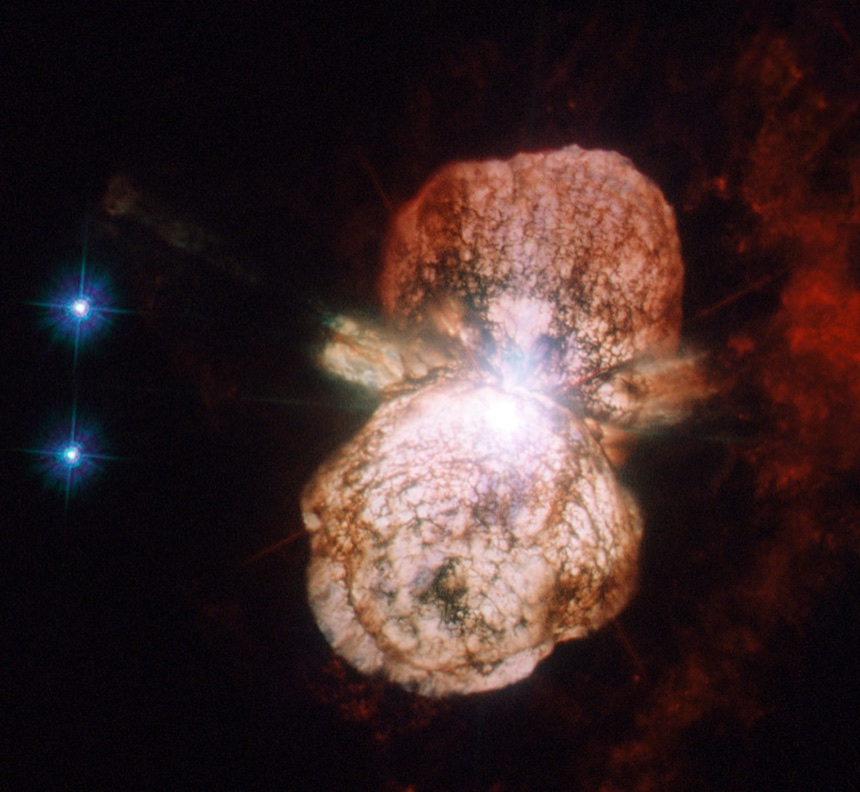
\includegraphics[width=0.78\textwidth,height=5.6cm,keepaspectratio]{../public/textures/nasa/sirius.jpg}\\[3pt]
{\footnotesize\itshape\color{orbitarMuted} Fotografie reală NASA/ESA (Telescopul Spațial Hubble): Steaua strălucitoare Sirius A și pitica albă Sirius B (punctul din stânga-jos).}
\end{center}


\begin{tcolorbox}[orbitardata, title={\textbf{Repere esențiale: Sirius A \& B (Luceafărul Câinelui)}}]
\small
\begin{itemize}[leftmargin=1.4em, itemsep=2pt, topsep=2pt]
  \item \textbf{Clasificare și orbită:} Stea \quad$\bullet$\quad \textbf{Distanță:} 8,6 ani-lumină
  \item \textbf{Dimensiuni și masă:} Sirius A este de 1,71 ori mai mare în diametru decât Soarele și de 25 de ori mai strălucitoare, în timp ce companionul Sirius B (o pitică albă) are masa Soarelui comprimată într-un glob doar cât Pământul! \quad$\bullet$\quad masă: 673000,000 $\times M_\oplus$
  \item \textbf{Gravitație și regim termic:} 22,000 $\times g_\oplus$ (215,82 m/s$^2$) \quad$\bullet$\quad temperatură medie: +9.667 $^\circ$C
  \item \textbf{Ciclu orbital și rotație:} perioadă orbitală (an): 18.299 zile ($\approx$ 50,10 ani pământești) \quad$\bullet$\quad rotație (zi): 16,00 ore (0,67 zile pământești)
  \item \textbf{Durata călătoriei de pe Pământ:} cu viteza luminii ($1c$): \emph{8 ani și 7 luni}; cu racheta ($50.000$ de kilometri pe oră): \emph{154.000 de ani}; cu avionul ($900$ de kilometri pe oră): \emph{10,8 miliarde de ani}; cu mașina ($100$ de kilometri pe oră): \emph{97 de miliarde de ani}.
  \item \textbf{Repere de scară și curiozitate:} Sirius A este ca un far uriaș alb-albăstrui de 25 de ori mai puternic decât Soarele, iar lângă el se rotește Sirius B (\quotedblbase{}Cățelușul\textquotedblright{}), o stea pitică albă mică doar cât Pământul, dar grea cât un Soare întreg! Materia din pitica albă Sirius B este atât de deasă și grea, încât o singură linguriță din ea ar cântări pe Pământ aproximativ 5 tone, adică tot atât cât un elefant african matur!
\end{itemize}
\end{tcolorbox}

\vspace{4pt}
\noindent\textbf{Prezentare generală și profil astrofizic.} Sirius (Alpha Canis Majoris), aflată la 8,6 ani-lumină, este un sistem binar format din Sirius A (stea albă de secvență principală, tip spectral A1V, aproximativ 9.940 K) și Sirius B (una dintre cele mai masive pitice albe cunoscute, cu temperatura de aproximativ 25.000 K), care se orbitează reciproc la fiecare 50,1 ani. Dacă privești cerul senin într-o seară de iarnă, sub centura constelației Orion vei vedea o stea care scânteiază în alb și albastru mai tare decât oricare alta: este Sirius! De fapt, Sirius ascunde un secret fascinant, întrucât nu este o singură stea, ci un sistem binar format din două stele care orbitează împreună! Sirius A este ca un far uriaș alb-albăstrui de 25 de ori mai puternic decât Soarele, iar lângă el se rotește Sirius B (\quotedblbase{}Cățelușul\textquotedblright{}), o stea pitică albă mică doar cât Pământul, dar grea cât un Soare întreg!

\medskip
\noindent\textbf{Scara cosmică și călătoria luminii în timp.} La scară astronomică, dimensiunile sale sunt impresionante: Sirius A este de 1,71 ori mai mare în diametru decât Soarele și de 25 de ori mai strălucitoare, în timp ce companionul Sirius B (o pitică albă) are masa Soarelui comprimată într-un glob doar cât Pământul! Totodată, privind astăzi spre Sirius A \& B (Luceafărul Câinelui), observăm practic trecutul îndepărtat al Universului, întrucât lumina sa a călătorit prin spațiu până la noi: Lumina albastră-albă de la Sirius pe care o vedem în această seară a plecat spre Pământ acum 8,6 ani!

\medskip
\noindent\textbf{Alcătuirea fizică și structura internă.} Privind în profunzimea sa, alcătuirea fizică este organizată pe mai multe straturi și regiuni distincte, fiecare având un rol bine definit în evoluția și dinamica acestui obiect cosmic. În primul rând se remarcă \textbf{Sirius A (Steaua Principală A1V)}, stea alb-albăstruie cu masa de 2,06 mase solare și luminozitate de 25,4 ori mai mare decât a Soarelui. În completarea acestui ansamblu întâlnim \textbf{Sirius B (Pitica Albă DA2)}, nucleu stelar colapsat cu raza de aproximativ 5.840 de kilometri (aproape cât Pământul) și masa de 1,018 mase solare.

\medskip
\noindent\textbf{Observații astronomice și istoricul explorării.} Friedrich Bessel a dedus în 1844 existența unui companion invizibil observând oscilațiile mișcării lui Sirius A, iar Alvan Graham Clark a observat direct pitica albă Sirius B în 1862. Materia din pitica albă Sirius B este atât de deasă și grea, încât o singură linguriță din ea ar cântări pe Pământ aproximativ 5 tone, adică tot atât cât un elefant african matur!

\vspace{6pt}
\begin{tcolorbox}[orbitarquiz, title={\textbf{Întrebare de verificare \#49: Sirius A \& B (Luceafărul Câinelui)}}]
\textbf{Ce tip de stea este companionul Sirius B care orbitează în jurul strălucitoarei Sirius A?}
\begin{itemize}[leftmargin=2.2em, itemsep=2pt, topsep=4pt]
  \item[$\square$ \textbf{A.}] O pitică albă extrem de densă, de mărimea Pământului dar cu masa Soarelui
  \item[$\square$ \textbf{B.}] O planetă de gheață
  \item[$\square$ \textbf{C.}] O supergigantă roșie
  \item[$\square$ \textbf{D.}] Un asteroid metalic
\end{itemize}
\vspace{2pt}
{\footnotesize\color{orbitarMuted}\textbf{Răspuns corect:} \textbf{A} (O pitică albă extrem de densă, de mărimea Pământului dar cu masa Soarelui). \emph{Sirius B este o pitică albă, reprezentând nucleul dens rămas dintr-o stea străveche, având masa Soarelui strânsă într-un volum cât Pământul.}}
\end{tcolorbox}
\clearpage


\section{Sistemul TRAPPIST-1 (7 Exoplanete)}
\label{sec:body-trappist1}
\vspace{-4pt}
{\large\itshape\color{orbitarAccent} Steaua pitică ultra-rece cu 7 planete stâncoase de mărimea Pământului (40 ani-lumină)}\\[4pt]


\begin{center}
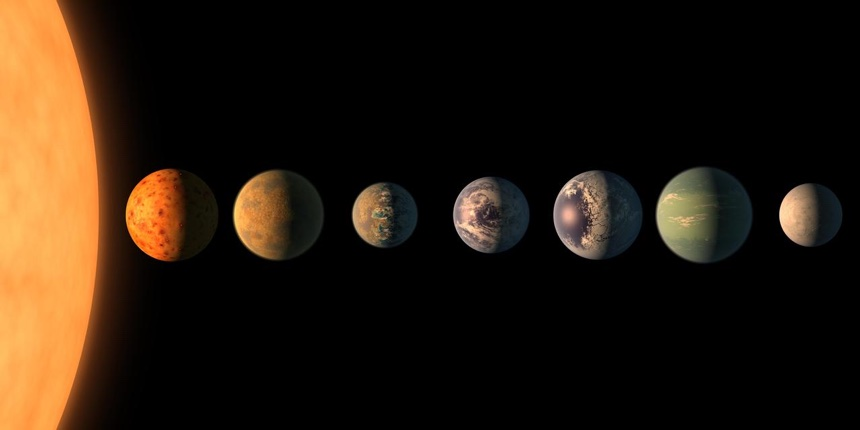
\includegraphics[width=0.78\textwidth,height=5.6cm,keepaspectratio]{../public/textures/nasa/trappist1.jpg}\\[3pt]
{\footnotesize\itshape\color{orbitarMuted} Randare științifică oficială NASA/JPL-Caltech (PIA21422): Cele 7 exoplanete stâncoase de mărimea Pământului din sistemul TRAPPIST-1.}
\end{center}


\begin{tcolorbox}[orbitardata, title={\textbf{Repere esențiale: Sistemul TRAPPIST-1 (7 Exoplanete)}}]
\small
\begin{itemize}[leftmargin=1.4em, itemsep=2pt, topsep=2pt]
  \item \textbf{Clasificare și orbită:} Sistem Exoplanetar / Exoplanetă \quad$\bullet$\quad \textbf{Distanță:} 40 de ani-lumină
  \item \textbf{Dimensiuni și masă:} Steaua TRAPPIST-1 este abia puțin mai mare decât planeta Jupiter (12\% din raza Soarelui), iar toate cele 7 planete ale sale încap pe o orbită mult mai strânsă decât orbita lui Mercur în jurul Soarelui! \quad$\bullet$\quad masă: 29800,000 $\times M_\oplus$
  \item \textbf{Gravitație și regim termic:} 0,930 $\times g_\oplus$ (9,12 m/s$^2$) \quad$\bullet$\quad temperatură medie: -22 $^\circ$C
  \item \textbf{Ciclu orbital și rotație:} perioadă orbitală (an): 6,1 zile pământești \quad$\bullet$\quad rotație (zi): 146,40 ore (6,10 zile pământești)
  \item \textbf{Durata călătoriei de pe Pământ:} cu viteza luminii ($1c$): \emph{40 de ani}; cu racheta ($50.000$ de kilometri pe oră): \emph{720.000 de ani}; cu avionul ($900$ de kilometri pe oră): \emph{50 de miliarde de ani}; cu mașina ($100$ de kilometri pe oră): \emph{450 de miliarde de ani}.
  \item \textbf{Repere de scară și curiozitate:} Dacă Sistemul nostru Solar este un teren mare de fotbal, întregul sistem TRAPPIST-1 cu toate cele 7 planete ale sale ar încăpea în cercul de la mijlocul terenului! Planetele sunt atât de aproape unele de altele, încât de pe una le-ai vedea pe celelalte pe cer mai mari decât vedem noi Luna! Toate cele 7 planete din sistemul TRAPPIST-1 sunt mai aproape de steaua lor decât este Mercur față de Soarele nostru, dar nu se ard fiindcă steaua lor este o pitică ultra-rece și blândă!
\end{itemize}
\end{tcolorbox}

\vspace{4pt}
\noindent\textbf{Prezentare generală și profil astrofizic.} Aflat la aproximativ 40 de ani-lumină în constelația Vărsătorul, sistemul TRAPPIST-1 conține o pitică ultra-rece (clasă M8V, masa aproximativ 0,09 mase solare) și șapte exoplanete telurice (TRAPPIST-1 b, c, d, e, f, g, h) cu perioade orbitale între 1,5 și 18,7 zile, aflate într-un lanț stabil de rezonanțe orbitale. TRAPPIST-1 este unul dintre cele mai uimitoare locuri din galaxie: o stea mică și roșiatică, înconjurată de o familie întreagă de 7 planete stâncoase, toate de mărimea Pământului! Trei dintre aceste planete (e, f și g) se află chiar în \quotedblbase{}zona potrivită\textquotedblright{}, unde ar putea exista oceane de apă lichidă! Dacă Sistemul nostru Solar este un teren mare de fotbal, întregul sistem TRAPPIST-1 cu toate cele 7 planete ale sale ar încăpea în cercul de la mijlocul terenului! Planetele sunt atât de aproape unele de altele, încât de pe una le-ai vedea pe celelalte pe cer mai mari decât vedem noi Luna!

\medskip
\noindent\textbf{Scara cosmică și călătoria luminii în timp.} La scară astronomică, dimensiunile sale sunt impresionante: Steaua TRAPPIST-1 este abia puțin mai mare decât planeta Jupiter (12\% din raza Soarelui), iar toate cele 7 planete ale sale încap pe o orbită mult mai strânsă decât orbita lui Mercur în jurul Soarelui! Totodată, privind astăzi spre Sistemul TRAPPIST-1 (7 Exoplanete), observăm practic trecutul îndepărtat al Universului, întrucât lumina sa a călătorit prin spațiu până la noi: Lumina de la sistemul TRAPPIST-1 pe care o vedem azi a plecat acum 40 de ani (în 1986), pe vremea când părinții tăi erau copii și se lansa stația spațială Mir!

\medskip
\noindent\textbf{Alcătuirea fizică și structura internă.} Privind în profunzimea sa, alcătuirea fizică este organizată pe mai multe straturi și regiuni distincte, fiecare având un rol bine definit în evoluția și dinamica acestui obiect cosmic. În primul rând se remarcă \textbf{Planetele Interioare (b, c, d)}, lumi stâncoase calde studiate în infraroșu de Telescopul Spațial James Webb (JWST) pentru detecția atmosferei. În strânsă legătură cu această componentă se află \textbf{Zona Locuibilă (TRAPPIST-1 e, f, g)}, trei exoplanete de mărimea Pământului aflate la distanța ideală pentru a susține apă lichidă la suprafață. În completarea acestui ansamblu întâlnim \textbf{Planeta Exterioară (TRAPPIST-1 h)}, lume înghețată cu perioada orbitală de 18,77 zile, situată la marginea sistemului compact.

\medskip
\noindent\textbf{Observații astronomice și istoricul explorării.} Descoperit în 2016--2017 de echipa condusă de Michaël Gillon cu telescopul TRAPPIST și telescopul spațial Spitzer; astăzi este ținta principală a Telescopului James Webb pentru studiul atmosferelor exoplanetare. Toate cele 7 planete din sistemul TRAPPIST-1 sunt mai aproape de steaua lor decât este Mercur față de Soarele nostru, dar nu se ard fiindcă steaua lor este o pitică ultra-rece și blândă!

\vspace{6pt}
\begin{tcolorbox}[orbitarquiz, title={\textbf{Întrebare de verificare \#50: Sistemul TRAPPIST-1 (7 Exoplanete)}}]
\textbf{Câte planete stâncoase de mărimea Pământului orbitează în jurul stelei TRAPPIST-1?}
\begin{itemize}[leftmargin=2.2em, itemsep=2pt, topsep=4pt]
  \item[$\square$ \textbf{A.}] 7 exoplanete stâncoase (dintre care 3 în zona locuibilă)
  \item[$\square$ \textbf{B.}] O singură planetă gazoasă
  \item[$\square$ \textbf{C.}] 100 de planete
  \item[$\square$ \textbf{D.}] Nicio planetă
\end{itemize}
\vspace{2pt}
{\footnotesize\color{orbitarMuted}\textbf{Răspuns corect:} \textbf{A} (7 exoplanete stâncoase (dintre care 3 în zona locuibilă)). \emph{Sistemul TRAPPIST-1 deține recordul pentru cele mai multe planete telurice de mărimea Pământului (7 planete: b, c, d, e, f, g, h) în jurul unei singure stele.}}
\end{tcolorbox}
\clearpage


\section{Exoplaneta 55 Cancri e (Janssen)}
\label{sec:body-cancri55e}
\vspace{-4pt}
{\large\itshape\color{orbitarAccent} \quotedblbase{}Planeta de Lavă și Diamant\textquotedblright{}, Super-Pământ incandescent (41 ani-lumină)}\\[4pt]


\begin{center}
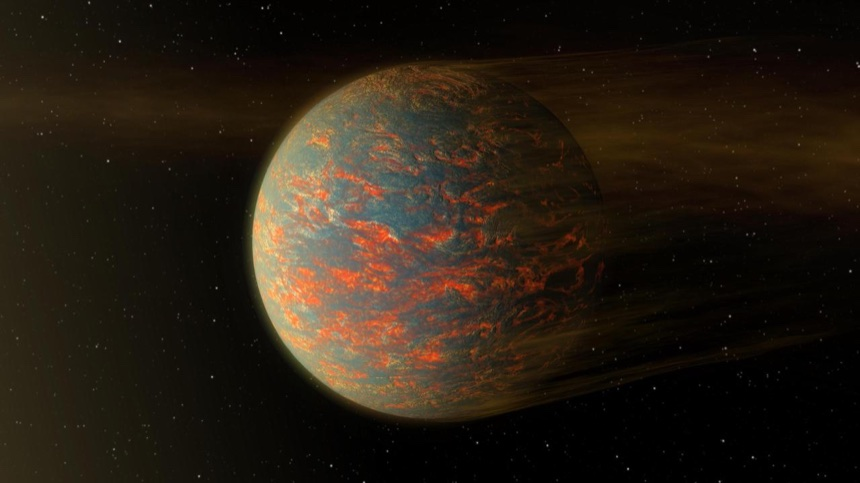
\includegraphics[width=0.78\textwidth,height=5.6cm,keepaspectratio]{../public/textures/nasa/cancri55e.jpg}\\[3pt]
{\footnotesize\itshape\color{orbitarMuted} Imagine științifică oficială NASA/JPL-Caltech (Telescopul Spitzer PIA20068): Exoplaneta incandescentă de lavă 55 Cancri e (Janssen).}
\end{center}


\begin{tcolorbox}[orbitardata, title={\textbf{Repere esențiale: Exoplaneta 55 Cancri e (Janssen)}}]
\small
\begin{itemize}[leftmargin=1.4em, itemsep=2pt, topsep=2pt]
  \item \textbf{Clasificare și orbită:} Sistem Exoplanetar / Exoplanetă \quad$\bullet$\quad \textbf{Distanță:} 41 de ani-lumină
  \item \textbf{Dimensiuni și masă:} Este un \quotedblbase{}Super-Pământ\textquotedblright{} cu diametrul de aproape 2 ori mai mare decât al Pământului și de 8 ori mai masiv! \quad$\bullet$\quad masă: 7,990 $\times M_\oplus$
  \item \textbf{Gravitație și regim termic:} 2,200 $\times g_\oplus$ (21,58 m/s$^2$) \quad$\bullet$\quad temperatură medie: +2.000 $^\circ$C
  \item \textbf{Ciclu orbital și rotație:} perioadă orbitală (an): 0,737 zile pământești \quad$\bullet$\quad rotație (zi): 17,67 ore (0,74 zile pământești)
  \item \textbf{Durata călătoriei de pe Pământ:} cu viteza luminii ($1c$): \emph{41 de ani}; cu racheta ($50.000$ de kilometri pe oră): \emph{738.000 de ani}; cu avionul ($900$ de kilometri pe oră): \emph{51 de miliarde de ani}; cu mașina ($100$ de kilometri pe oră): \emph{460 de miliarde de ani}.
  \item \textbf{Repere de scară și curiozitate:} Dacă Pământul este o bilă albastră acoperită cu oceane de apă răcoroasă, 55 Cancri e este o bilă incandescentă acoperită cu oceane de magmă vulcanică și nori de rocă vaporizată! Pe 55 Cancri e, anul nou vine înainte să se termine o singură zi de pe Pământ: planeta dă ocol stelei sale în doar 17 ore și 40 de minute!
\end{itemize}
\end{tcolorbox}

\vspace{4pt}
\noindent\textbf{Prezentare generală și profil astrofizic.} 55 Cancri e (numită oficial Janssen) este o exoplanetă de tip Super-Pământ aflată la 41 de ani-lumină în constelația Racul. Orbitează la doar 0,015 UA de steaua 55 Cancri A, fiind blocată mareic: emisfera diurnă atinge aproximativ 2.000 $^\circ$C (acoperită de un ocean global de magmă), iar observațiile JWST din 2024 au confirmat prezența unei atmosfere secundare bogate în CO și CO$_2$ degajate din oceanul de lavă. Imaginează-ți o planetă de aproape două ori mai mare decât Pământul, atât de apropiată de steaua ei încât un an întreg acolo durează doar 17 ore și jumătate! Pe partea îndreptată spre stea, stâncile s-au topit într-un ocean uriaș de lavă strălucitoare, iar în adâncuri carbonul presat poate forma straturi întregi de diamant! Dacă Pământul este o bilă albastră acoperită cu oceane de apă răcoroasă, 55 Cancri e este o bilă incandescentă acoperită cu oceane de magmă vulcanică și nori de rocă vaporizată!

\medskip
\noindent\textbf{Scara cosmică și călătoria luminii în timp.} La scară astronomică, dimensiunile sale sunt impresionante: Este un \quotedblbase{}Super-Pământ\textquotedblright{} cu diametrul de aproape 2 ori mai mare decât al Pământului și de 8 ori mai masiv! Totodată, privind astăzi spre Exoplaneta 55 Cancri e (Janssen), observăm practic trecutul îndepărtat al Universului, întrucât lumina sa a călătorit prin spațiu până la noi: Lumina de la sistemul 55 Cancri pe care o vedem azi a plecat acum 41 de ani (în 1985)!

\medskip
\noindent\textbf{Alcătuirea fizică și structura internă.} Privind în profunzimea sa, alcătuirea fizică este organizată pe mai multe straturi și regiuni distincte, fiecare având un rol bine definit în evoluția și dinamica acestui obiect cosmic. În primul rând se remarcă \textbf{Ocean Global de Magmă}, suprafață de silicați topiți pe emisfera diurnă, la temperaturi de peste 2.000 $^\circ$C. În strânsă legătură cu această componentă se află \textbf{Manta Bogată în Carbon și Siliciu}, unde presiunile extreme din interiorul unei planete de 8 mase terestre pot cristaliza carbonul sub formă de diamant. În completarea acestui ansamblu întâlnim \textbf{Atmosferă Volatilă de Roci și Gaze}, atmosferă densă de monoxid și dioxid de carbon detectată de Telescopul Spațial James Webb în 2024.

\medskip
\noindent\textbf{Observații astronomice și istoricul explorării.} Descoperită în 2004 prin metoda vitezelor radiale și observată în tranzit de telescoapele Spitzer, Hubble, CHEOPS și James Webb (2024). Pe 55 Cancri e, anul nou vine înainte să se termine o singură zi de pe Pământ: planeta dă ocol stelei sale în doar 17 ore și 40 de minute!

\vspace{6pt}
\begin{tcolorbox}[orbitarquiz, title={\textbf{Întrebare de verificare \#51: Exoplaneta 55 Cancri e (Janssen)}}]
\textbf{De ce este suprafața exoplanetei 55 Cancri e acoperită de un ocean de lavă topită?}
\begin{itemize}[leftmargin=2.2em, itemsep=2pt, topsep=4pt]
  \item[$\square$ \textbf{A.}] Pentru că orbitează extrem de aproape de steaua ei (un an durează doar aproximativ 18 ore), la aproximativ 2.000 $^\circ$C
  \item[$\square$ \textbf{B.}] Pentru că este făcută din gheață
  \item[$\square$ \textbf{C.}] Pentru că nu are nicio stea în apropiere
  \item[$\square$ \textbf{D.}] Pentru că se află în Centura Kuiper
\end{itemize}
\vspace{2pt}
{\footnotesize\color{orbitarMuted}\textbf{Răspuns corect:} \textbf{A} (Pentru că orbitează extrem de aproape de steaua ei (un an durează doar aproximativ 18 ore), la aproximativ 2.000 $^\circ$C). \emph{Fiind la doar 0,015 UA de steaua ei, 55 Cancri e este încălzită la aproximativ 2.000 $^\circ$C, topind rocile de la suprafață într-un ocean global de magmă.}}
\end{tcolorbox}
\clearpage


\section{Roiul Stelar Pleiadele (\quotedblbase{}Cloșca cu Pui\textquotedblright{})}
\label{sec:body-pleiades}
\vspace{-4pt}
{\large\itshape\color{orbitarAccent} Roiul deschis M45 de stele tinere albastre din Taurul (444 ani-lumină)}\\[4pt]


\begin{center}
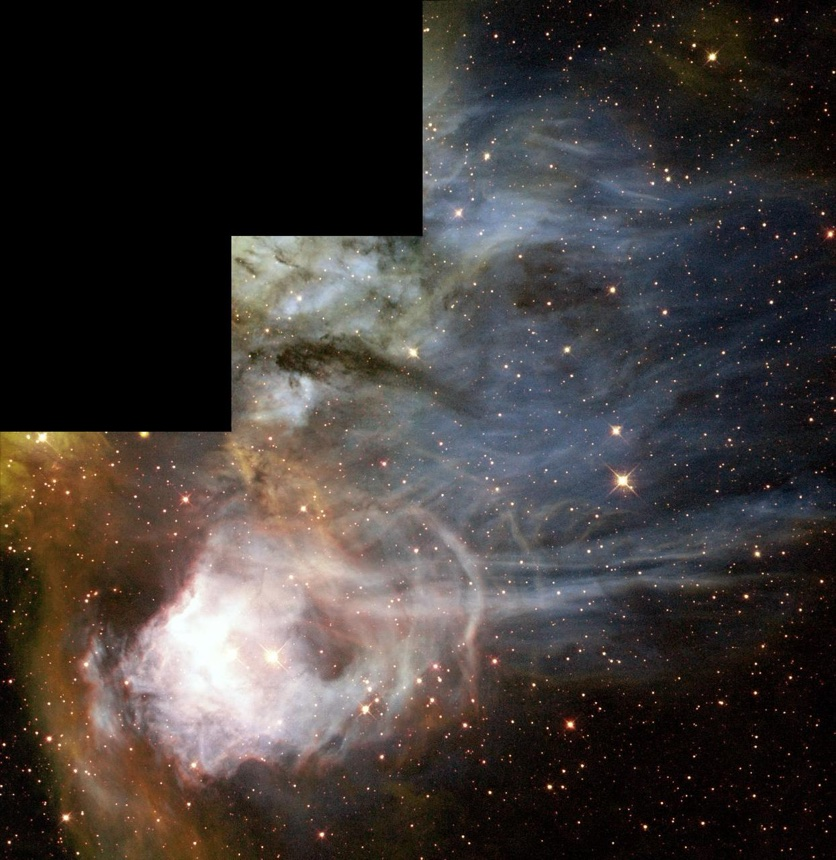
\includegraphics[width=0.78\textwidth,height=5.6cm,keepaspectratio]{../public/textures/nasa/pleiades.jpg}\\[3pt]
{\footnotesize\itshape\color{orbitarMuted} Fotografie reală NASA/JPL-Caltech/Hubble (PIA04225): Roiul stelar deschis Pleiadele (M45, \quotedblbase{}Cloșca cu Pui\textquotedblright{}).}
\end{center}


\begin{tcolorbox}[orbitardata, title={\textbf{Repere esențiale: Roiul Stelar Pleiadele (\quotedblbase{}Cloșca cu Pui\textquotedblright{})}}]
\small
\begin{itemize}[leftmargin=1.4em, itemsep=2pt, topsep=2pt]
  \item \textbf{Clasificare și orbită:} Roi Stelar Deschis \quad$\bullet$\quad \textbf{Distanță:} 444 de ani-lumină
  \item \textbf{Dimensiuni și masă:} Roiul Pleiadelor conține peste 1.000 de stele tinere răspândite pe o lățime de aproximativ 17 ani-lumină (de 17 ori mai mare decât întregul Nor al lui Oort)! \quad$\bullet$\quad masă: 266000000,000 $\times M_\oplus$
  \item \textbf{Gravitație și regim termic:} 1,000 $\times g_\oplus$ (9,81 m/s$^2$) \quad$\bullet$\quad temperatură medie: +12.000 $^\circ$C
  \item \textbf{Ciclu orbital și rotație:} perioadă orbitală (an): Orbitează centrul Căii Lactee (aproximativ 230 de milioane de ani) \quad$\bullet$\quad rotație (zi): 24,00 ore (1,00 zile pământești)
  \item \textbf{Durata călătoriei de pe Pământ:} cu viteza luminii ($1c$): \emph{444 de ani}; cu racheta ($50.000$ de kilometri pe oră): \emph{8 milioane de ani}; cu avionul ($900$ de kilometri pe oră): \emph{550 de miliarde de ani}; cu mașina ($100$ de kilometri pe oră): \emph{5.000 de miliarde de ani}.
  \item \textbf{Repere de scară și curiozitate:} Pleiadele sunt ca o \quotedblbase{}grădiniță de stele-frați\textquotedblright{} născute din același nor cosmic acum 100 de milioane de ani, în epoca în care pe Pământ încă trăiau dinozaurii! Lumina albastră de la \quotedblbase{}Cloșca cu Pui\textquotedblright{} călătorește prin spațiu timp de 444 de ani până ajunge la noi: razele pe care le vezi diseară au plecat de acolo pe vremea lui Mihai Viteazul!
\end{itemize}
\end{tcolorbox}

\vspace{4pt}
\noindent\textbf{Prezentare generală și profil astrofizic.} Pleiadele (Messier 45 / \quotedblbase{}Cloșca cu Pui\textquotedblright{}), situate la aproximativ 444 de ani-lumină în constelația Taurul, reprezintă cel mai cunoscut roi stelar deschis de pe cer. Este dominat de gigante albastre extrem de luminoase (Alcyone, Atlas, Electra, Maia, Merope, Taygeta, Pleione) care iluminează o nebuloasă de reflexie albastră la trecerea printr-un nor interstelar de praf. Când privești cerul nopții toamna sau iarna, poți vedea cu ochiul liber un buchet mic și sclipitor de 7 stele albastre care stau strânse împreună. În România, bunicii noștri le-au numit cu drag \quotedblbase{}Cloșca cu Pui\textquotedblright{} sau \quotedblbase{}Găinușa\textquotedblright{}! Prin telescop însă descoperim că acolo sunt peste 1.000 de stele tinere și fierbinți, învăluite într-un voal albastru de praf stelar! Pleiadele sunt ca o \quotedblbase{}grădiniță de stele-frați\textquotedblright{} născute din același nor cosmic acum 100 de milioane de ani, în epoca în care pe Pământ încă trăiau dinozaurii!

\medskip
\noindent\textbf{Scara cosmică și călătoria luminii în timp.} La scară astronomică, dimensiunile sale sunt impresionante: Roiul Pleiadelor conține peste 1.000 de stele tinere răspândite pe o lățime de aproximativ 17 ani-lumină (de 17 ori mai mare decât întregul Nor al lui Oort)! Totodată, privind astăzi spre Roiul Stelar Pleiadele (\quotedblbase{}Cloșca cu Pui\textquotedblright{}), observăm practic trecutul îndepărtat al Universului, întrucât lumina sa a călătorit prin spațiu până la noi: Lumina de la Pleiade (\quotedblbase{}Cloșca cu Pui\textquotedblright{}) pe care o vedem azi pe cer a plecat acum 444 de ani, în anul 1582, pe vremea lui Mihai Viteazul!

\medskip
\noindent\textbf{Alcătuirea fizică și structura internă.} Privind în profunzimea sa, alcătuirea fizică este organizată pe mai multe straturi și regiuni distincte, fiecare având un rol bine definit în evoluția și dinamica acestui obiect cosmic. În primul rând se remarcă \textbf{Cele 7 Surori (Gigante Albastre B)}, stele masive și tinere (aproximativ 100 de milioane de ani), fiecare de sute de ori mai luminoasă decât Soarele. În completarea acestui ansamblu întâlnim \textbf{Nebuloasa de Reflexie Merope (NGC 1435)}, nor fin de praf interstelar care împrăștie lumina albastră a stelelor din roi.

\medskip
\noindent\textbf{Observații astronomice și istoricul explorării.} Cunoscute din antichitate în toate culturile lumii (și în astronomia populară românească drept \quotedblbase{}Cloșca cu Pui\textquotedblright{}), Pleiadele au fost desenate pentru prima dată prin telescop de Galileo Galilei în 1610 și catalogate de Charles Messier ca M45 în 1769. Lumina albastră de la \quotedblbase{}Cloșca cu Pui\textquotedblright{} călătorește prin spațiu timp de 444 de ani până ajunge la noi: razele pe care le vezi diseară au plecat de acolo pe vremea lui Mihai Viteazul!

\vspace{6pt}
\begin{tcolorbox}[orbitarquiz, title={\textbf{Întrebare de verificare \#52: Roiul Stelar Pleiadele (\quotedblbase{}Cloșca cu Pui\textquotedblright{})}}]
\textbf{Cum este numit roiul stelar Pleiadele (M45) în tradiția populară românească și acum câți ani a plecat lumina lui spre noi?}
\begin{itemize}[leftmargin=2.2em, itemsep=2pt, topsep=4pt]
  \item[$\square$ \textbf{A.}] \quotedblbase{}Cloșca cu Pui\textquotedblright{}, iar lumina a plecat acum aproximativ 444 de ani
  \item[$\square$ \textbf{B.}] \quotedblbase{}Carul Mare\textquotedblright{}, la 10 kilometri distanță
  \item[$\square$ \textbf{C.}] \quotedblbase{}Luceafărul de Dimineață\textquotedblright{}, la 8 minute-lumină
  \item[$\square$ \textbf{D.}] \quotedblbase{}Calea Robilor\textquotedblright{}, la 1 miliard de ani-lumină
\end{itemize}
\vspace{2pt}
{\footnotesize\color{orbitarMuted}\textbf{Răspuns corect:} \textbf{A} (\quotedblbase{}Cloșca cu Pui\textquotedblright{}, iar lumina a plecat acum aproximativ 444 de ani). \emph{În tradiția românească, Pleiadele sunt numite \quotedblbase{}Cloșca cu Pui\textquotedblright{} (sau \quotedblbase{}Găinușa\textquotedblright{}), iar la distanța de 444 de ani-lumină, lumina lor a plecat spre Pământ în secolul al XVI-lea.}}
\end{tcolorbox}
\clearpage


\section{Betelgeuse (Supergiganta Roșie)}
\label{sec:body-betelgeuse}
\vspace{-4pt}
{\large\itshape\color{orbitarAccent} Steaua colosală din Orion, de aproximativ 700 de ori mai mare decât Soarele (640 ani-lumină)}\\[4pt]


\begin{center}
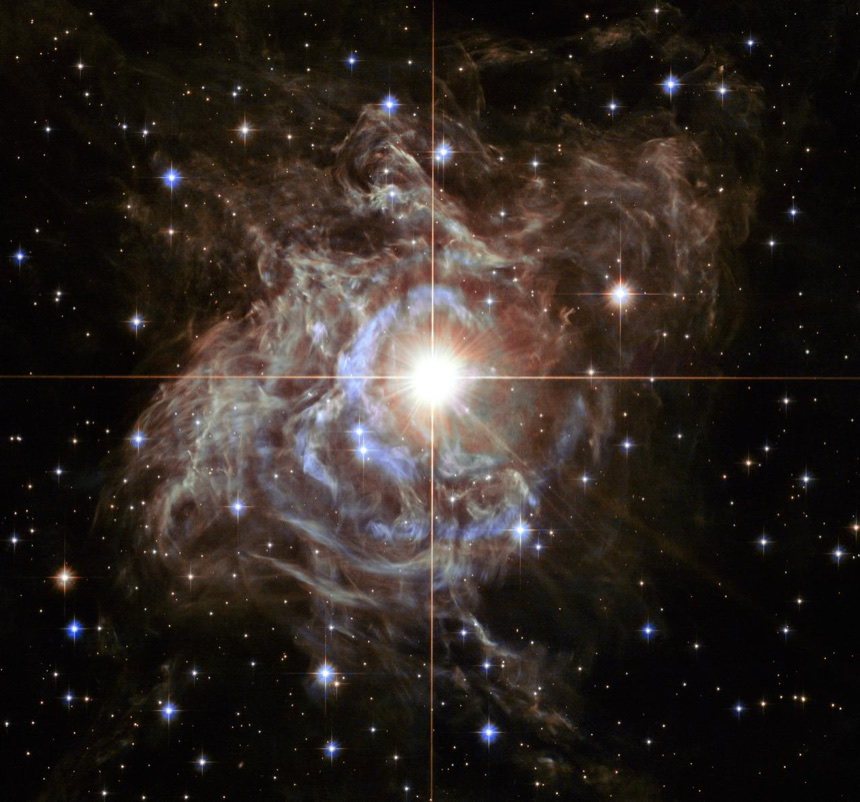
\includegraphics[width=0.78\textwidth,height=5.6cm,keepaspectratio]{../public/textures/nasa/betelgeuse.jpg}\\[3pt]
{\footnotesize\itshape\color{orbitarMuted} Imagine reală NASA/ESA (Telescopul Spațial Hubble): Supergiganta roșie Betelgeuse din constelația Orion.}
\end{center}


\begin{tcolorbox}[orbitardata, title={\textbf{Repere esențiale: Betelgeuse (Supergiganta Roșie)}}]
\small
\begin{itemize}[leftmargin=1.4em, itemsep=2pt, topsep=2pt]
  \item \textbf{Clasificare și orbită:} Stea \quad$\bullet$\quad \textbf{Distanță:} 640 de ani-lumină
  \item \textbf{Dimensiuni și masă:} Betelgeuse are un diametru de aproximativ 700 de ori mai mare decât Soarele! Dacă am așeza-o în centrul Sistemului Solar, marginea ei ar înghiți Mercur, Venus, Pământul, Marte și ar ajunge până la orbita lui Jupiter! \quad$\bullet$\quad masă: 5500000,000 $\times M_\oplus$
  \item \textbf{Gravitație și regim termic:} Microgravitație / Imponderabilitate ($\approx 0\,g$) \quad$\bullet$\quad temperatură medie: +3.327 $^\circ$C
  \item \textbf{Ciclu orbital și rotație:} perioadă orbitală (an): Orbitează centrul Căii Lactee (aproximativ 230 de milioane de ani) \quad$\bullet$\quad rotație (zi): 720,00 ore (30,00 zile pământești)
  \item \textbf{Durata călătoriei de pe Pământ:} cu viteza luminii ($1c$): \emph{640 de ani}; cu racheta ($50.000$ de kilometri pe oră): \emph{11,5 milioane de ani}; cu avionul ($900$ de kilometri pe oră): \emph{800 de miliarde de ani}; cu mașina ($100$ de kilometri pe oră): \emph{7.200 de miliarde de ani}.
  \item \textbf{Repere de scară și curiozitate:} Dacă Soarele nostru ar fi o minge mică de ping-pong, supergiganta Betelgeuse ar fi un balon gonflabil înalt cât o clădire cu 9 etaje (28 de metri diametru)! În anul 2019, Betelgeuse s-a întunecat brusc pentru câteva luni, iar astronomii au descoperit cu telescopul Hubble că steaua \quotedblbase{}strănutase\textquotedblright{} un nor uriaș de praf cosmic care îi umbrea fața!
\end{itemize}
\end{tcolorbox}

\vspace{4pt}
\noindent\textbf{Prezentare generală și profil astrofizic.} Betelgeuse (Alpha Orionis), aflată la aproximativ 640 de ani-lumină, este o supergigantă roșie variabilă semiregulată (clasă spectrală M1--M2 Ia-ab) aflată în ultimele etape ale evoluției sale stelare. Cu o rază de aproximativ 700 raze solare și o luminozitate de aproximativ 100.000 de ori mai mare decât a Soarelui, Betelgeuse își fuzionează elementele grele din nucleu și va sfârși într-o supernovă spectaculoasă în următorii aproximativ 100.000 de ani. În umărul stâng al constelației Orion strălucește o stea portocalie-roșiatică de o mărime aproape de neimaginat: Betelgeuse! Este o supergigantă roșie atât de uriașă, încât înăuntrul ei ar încăpea sute de milioane de Sori! Dacă Betelgeuse ar fi pusă în locul Soarelui nostru, Pământul și chiar Marte s-ar afla în interiorul stelei! Dacă Soarele nostru ar fi o minge mică de ping-pong, supergiganta Betelgeuse ar fi un balon gonflabil înalt cât o clădire cu 9 etaje (28 de metri diametru)!

\medskip
\noindent\textbf{Scara cosmică și călătoria luminii în timp.} La scară astronomică, dimensiunile sale sunt impresionante: Betelgeuse are un diametru de aproximativ 700 de ori mai mare decât Soarele! Dacă am așeza-o în centrul Sistemului Solar, marginea ei ar înghiți Mercur, Venus, Pământul, Marte și ar ajunge până la orbita lui Jupiter! Totodată, privind astăzi spre Betelgeuse (Supergiganta Roșie), observăm practic trecutul îndepărtat al Universului, întrucât lumina sa a călătorit prin spațiu până la noi: Lumina roșiatică de la Betelgeuse pe care o vedem azi a plecat acum 640 de ani, în anul 1386, chiar în anul în care a început domnia lui Mircea cel Bătrân în Țara Românească!

\medskip
\noindent\textbf{Alcătuirea fizică și structura internă.} Privind în profunzimea sa, alcătuirea fizică este organizată pe mai multe straturi și regiuni distincte, fiecare având un rol bine definit în evoluția și dinamica acestui obiect cosmic. În primul rând se remarcă \textbf{Fotosferă Convectivă Uriașă}, celule gigantice de convecție (fiecare cât orbita Pământului) care fac suprafața stelei să pulseze și să își schimbe strălucirea. În completarea acestui ansamblu întâlnim \textbf{Înveliș Circumstelar de Praf}, nori extinși de silicați și alumină expulzați de vântul stelar puternic până la zeci de raze stelare.

\medskip
\noindent\textbf{Observații astronomice și istoricul explorării.} În 1920, Betelgeuse a devenit prima stea (în afară de Soare) al cărei diametru unghiular a fost măsurat direct (de Michelson și Pease la Observatorul Mount Wilson); în 2019--2020 a trecut prin \quotedblbase{}Marea Întunecare\textquotedblright{} studiată de Hubble și VLT. În anul 2019, Betelgeuse s-a întunecat brusc pentru câteva luni, iar astronomii au descoperit cu telescopul Hubble că steaua \quotedblbase{}strănutase\textquotedblright{} un nor uriaș de praf cosmic care îi umbrea fața!

\vspace{6pt}
\begin{tcolorbox}[orbitarquiz, title={\textbf{Întrebare de verificare \#53: Betelgeuse (Supergiganta Roșie)}}]
\textbf{Până unde s-ar întinde supergiganta roșie Betelgeuse dacă ar fi așezată în locul Soarelui nostru?}
\begin{itemize}[leftmargin=2.2em, itemsep=2pt, topsep=4pt]
  \item[$\square$ \textbf{A.}] Ar înghiți Mercur, Venus, Pământul și Marte, ajungând aproape de orbita lui Jupiter
  \item[$\square$ \textbf{B.}] Ar fi mai mică decât Luna
  \item[$\square$ \textbf{C.}] Ar ajunge doar până la Stația Spațială Internațională
  \item[$\square$ \textbf{D.}] Ar fi de mărimea unui asteroid
\end{itemize}
\vspace{2pt}
{\footnotesize\color{orbitarMuted}\textbf{Răspuns corect:} \textbf{A} (Ar înghiți Mercur, Venus, Pământul și Marte, ajungând aproape de orbita lui Jupiter). \emph{Având o rază de aproximativ 700 de ori mai mare decât a Soarelui (aproximativ 3,5 UA), Betelgeuse ar depăși orbita lui Marte și Centura de Asteroizi, apropiindu-se de Jupiter.}}
\end{tcolorbox}
\clearpage


% SPDX-License-Identifier: GPL-3.0-or-later
\chapter{Nebuloase, Găuri Negre și Galaxii}
\label{chap:galaxii}

În \textbf{Orizontul 3 („Calea Lactee și Galaxii”)}, camera din \textbf{Orbitar} se ridică la mii și milioane de ani-lumină pentru a cuprinde arhitectura la scară mare a Universului: \textbf{nebuloasele difuze} (maternitățile cosmice unde se nasc mii de stele noi), \textbf{nebuloasele planetare și rămășițele de supernovă} (care îmbogățesc galaxia cu elementele chimice ale vieții), \textbf{gaura neagră supermasivă Sagittarius A*} din inima galaxiei noastre, \textbf{Calea Lactee} și \textbf{galaxiile vecine sau îndepărtate}.

\section*{De la Maternitățile de Stele la Galaxiile Spirale}

\begin{itemize}[leftmargin=1.5em, itemsep=3pt]
  \item \textbf{Nebuloasele de emisie și formare stelară (\emph{Orion M42, Stâlpii Creației M16, Carina NGC 3372}):} nori colosali de hidrogen rece și praf cosmic în care gravitația strânge materia în noduri dense numite protostele.
  \item \textbf{Nebuloasele planetare (\emph{Inelul M57, Helix NGC 7293}):} straturile exterioare luminoase de gaz eliberate pașnic la finalul vieții de stelele de mărimea Soarelui, lăsând în centru o \emph{pitică albă}.
  \item \textbf{Rămășițele de supernovă și pulsarii (\emph{Nebuloasa Crabului M1}):} explozii cataclismice ale stelelor masive, în urma cărora nucleul colapsează într-o \emph{stea neutronică (pulsar)} sau într-o \emph{gaură neagră}.
  \item \textbf{Roiurile globulare (precum \emph{Omega Centauri}):} sfere străvechi de până la $10\text{ milioane de stele}$ care orbitează în haloul Căii Lactee.
  \item \textbf{Galaxiile (\emph{Calea Lactee, Marele Nor al lui Magellan, Andromeda M31, Triunghiul M33, Vâltoarea M51, Sombrero M104}):} insule cosmice legate gravitațional, formate din zeci sau sute de miliarde de stele, gaz, praf, o gaură neagră supermasivă centrală și un halou invizibil de materie întunecată.
\end{itemize}

\begin{center}
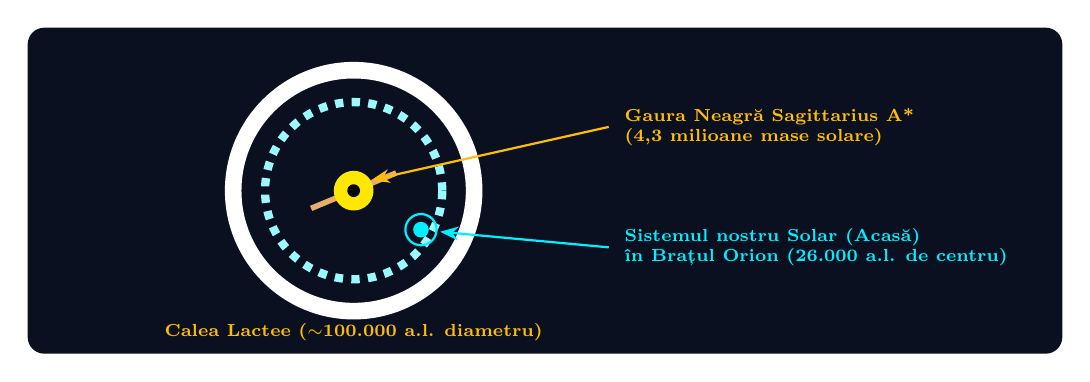
\begin{tikzpicture}[scale=0.90, every node/.style={transform shape}]
  \fill[orbitarSpaceBg, rounded corners=6pt] (-1.0,-2.3) rectangle (13.6,2.3);

  % Discul Căii Lactee văzut de sus (schematic)
  \coordinate (G) at (3.6,0);
  \draw[white!20, line width=6pt] (G) circle (1.7cm);
  \draw[orbitarCyan!40, line width=3pt, dashed] (G) circle (1.25cm);
  \draw[orbitarAmber!60, line width=2pt] ($(G)+(-0.6,-0.25)$) -- ($(G)+(0.6,0.25)$);
  \fill[yellow!90!orange] (G) circle (0.28cm);
  \fill[black] (G) circle (0.09cm);
  \node[amber!90!yellow, font=\scriptsize\bfseries] at (3.6,-2.0) {Calea Lactee ($\sim$100.000 a.l. diametru)};

  % Poziția Soarelui în Brațul Orion
  \fill[orbitarCyan] ($(G)+(0.95,-0.55)$) circle (0.11cm);
  \draw[orbitarCyan, line width=0.8pt] ($(G)+(0.95,-0.55)$) circle (0.22cm);
  \draw[-{Stealth}, orbitarCyan, line width=0.8pt] (7.2,-0.8) -- ($(G)+(1.22,-0.58)$);
  \node[orbitarCyan, font=\scriptsize\bfseries, anchor=west, align=left] at (7.3,-0.8) {Sistemul nostru Solar (Acasă)\\în Brațul Orion (26.000 a.l. de centru)};

  % Săgeată spre Sagittarius A*
  \draw[-{Stealth}, amber!90!yellow, line width=0.8pt] (7.2,0.9) -- ($(G)+(0.25,0.15)$);
  \node[amber!90!yellow, font=\scriptsize\bfseries, anchor=west, align=left] at (7.3,0.9) {Gaura Neagră Sagittarius A*\\(4,3 milioane mase solare)};
\end{tikzpicture}
\end{center}

\begin{table}[H]
\centering
\small
\caption{Cele 13 nebuloase, găuri negre și galaxii din Orizontul 3 în Orbitar}
\resizebox{\textwidth}{!}{%
\begin{tabular}{@{}lll@{}}
\toprule
\textbf{Obiect Cosmic} & \textbf{Categorie} & \textbf{Distanță / Scară în Ani-Lumină} \\
\midrule
Nebuloasa Orion (M42) & Nebuloasă Cosmică & 1.344 de ani-lumină \\
Stâlpii Creației (Nebuloasa Vulturului M16) & Nebuloasă Cosmică & 6.500 de ani-lumină \\
Sagittarius A* (Gaura Neagră Supermasivă) & Gaură Neagră Supermasivă & 26.000 de ani-lumină \\
Calea Lactee (Galaxia Noastră) & Galaxie & Diametru aproximativ 100.000 ani-lumină (Soarele la 26.000 a.l. de centru) \\
Galaxia Andromeda (M31) & Galaxie & 2,54 de milioane de ani-lumină \\
Nebuloasa Carina (\quotedblbase{}Stâncile Cosmice\textquotedblright{}, NGC 3372) & Nebuloasă Cosmică & 7.500 de ani-lumină \\
Nebuloasa Crabului (M1) & Nebuloasă Cosmică & 6.500 de ani-lumină \\
Nebuloasa Inelul (M57) & Nebuloasă Cosmică & 2.300 de ani-lumină \\
Nebuloasa Helix (\quotedblbase{}Ochiul lui Dumnezeu\textquotedblright{}, NGC 7293) & Nebuloasă Cosmică & 650 de ani-lumină \\
Marele Nor al lui Magellan & Galaxie & 160.000 de ani-lumină \\
Galaxia Triunghiului (M33) & Galaxie & 2,73 de milioane de ani-lumină \\
Galaxia Vâltoarea (M51) & Galaxie & 23,5 milioane de ani-lumină \\
Galaxia Sombrero (M104) & Galaxie & 29,3 milioane de ani-lumină \\
\bottomrule
\end{tabular}%
}
\end{table}

\clearpage

\section{Nebuloasa Orion (M42)}
\label{sec:body-orion_nebula}
\vspace{-4pt}
{\large\itshape\color{orbitarAccent} Cea mai apropiată maternitate stelară masivă, studiată de James Webb (1.344 ani-lumină)}\\[4pt]


\begin{center}
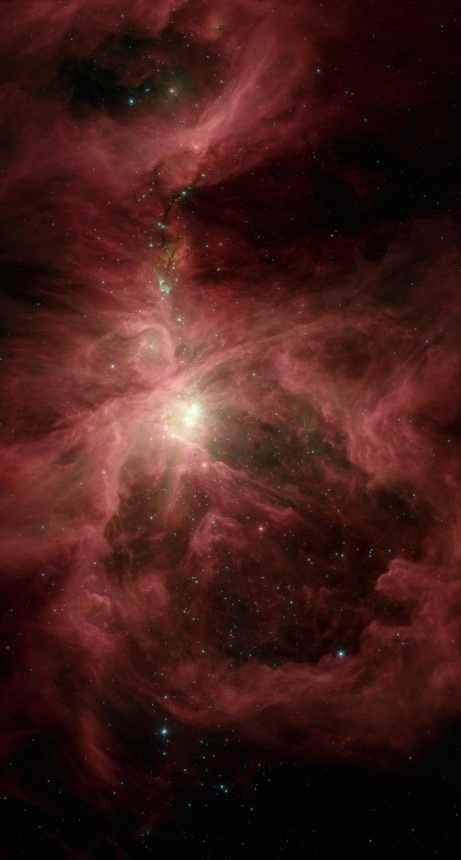
\includegraphics[width=0.78\textwidth,height=5.6cm,keepaspectratio]{../public/textures/nasa/orion_nebula.jpg}\\[3pt]
{\footnotesize\itshape\color{orbitarMuted} Fotografie reală NASA/JPL-Caltech/ESA (Hubble \& Spitzer PIA08653): Maternitatea stelară Nebuloasa Orion (M42).}
\end{center}


\begin{tcolorbox}[orbitardata, title={\textbf{Repere esențiale: Nebuloasa Orion (M42)}}]
\small
\begin{itemize}[leftmargin=1.4em, itemsep=2pt, topsep=2pt]
  \item \textbf{Clasificare și orbită:} Nebuloasă Cosmică \quad$\bullet$\quad \textbf{Distanță:} 1.344 de ani-lumină
  \item \textbf{Dimensiuni și masă:} Nebuloasa Orion măsoară 24 de ani-lumină de la un capăt la altul și este de 24 de ori mai lată decât întregul Sistem Solar împreună cu Norul lui Oort! \quad$\bullet$\quad masă: 666000000,000 $\times M_\oplus$
  \item \textbf{Gravitație și regim termic:} 0,100 $\times g_\oplus$ (0,98 m/s$^2$) \quad$\bullet$\quad temperatură medie: +9.700 $^\circ$C
  \item \textbf{Ciclu orbital și rotație:} perioadă orbitală (an): Orbitează centrul Căii Lactee (aproximativ 230 de milioane de ani) \quad$\bullet$\quad rotație (zi): 24,00 ore (1,00 zile pământești)
  \item \textbf{Durata călătoriei de pe Pământ:} cu viteza luminii ($1c$): \emph{1.344 de ani}; cu racheta ($50.000$ de kilometri pe oră): \emph{24 de milioane de ani}; cu avionul ($900$ de kilometri pe oră): \emph{1.680 de miliarde de ani}; cu mașina ($100$ de kilometri pe oră): \emph{15.000 de miliarde de ani}.
  \item \textbf{Repere de scară și curiozitate:} Nebuloasa Orion este ca un cuib luminos din vată de zahăr cosmică, lat de 24 de ani-lumină, în mijlocul căruia patru stele-bebeluș foarte puternice (\quotedblbase{}Trapezul\textquotedblright{}) aprind întregul nor ca niște reflectoare! Telescopul Spațial James Webb a privit cu ochii săi în infraroșu în interiorul Nebuloasei Orion și a fotografiat discuri de praf (\quotedblbase{}proplyde\textquotedblright{}) în jurul stelelor nou-născute, exact acolo unde se formează viitoare planete!
\end{itemize}
\end{tcolorbox}

\vspace{4pt}
\noindent\textbf{Prezentare generală și profil astrofizic.} Nebuloasa Orion (Messier 42 / NGC 1976), situată la 1.344 de ani-lumină, este cea mai strălucitoare nebuloasă difuză de emisie și reflexie de pe cer (vizibilă chiar și cu ochiul liber, magnitudine 4,0). În centrul ei, roiul tânăr Trapezium ionizează hidrogenul și oxigenul din jur, iar observațiile JWST NIRCam au dezvăluit filamente moleculare, jeturi protostelare și discuri protoplanetare. Sub cele trei stele din \quotedblbase{}Centura lui Orion\textquotedblright{} se află un nor cosmic uriaș, strălucitor în nuanțe de roz, violet și turcoaz: Nebuloasa Orion! Este o adevărată \quotedblbase{}maternitate de stele\textquotedblright{}, un loc fermecat în care din nori de gaz și praf cosmic se nasc chiar acum sute de sori noi și sisteme solare tinere! Nebuloasa Orion este ca un cuib luminos din vată de zahăr cosmică, lat de 24 de ani-lumină, în mijlocul căruia patru stele-bebeluș foarte puternice (\quotedblbase{}Trapezul\textquotedblright{}) aprind întregul nor ca niște reflectoare!

\medskip
\noindent\textbf{Scara cosmică și călătoria luminii în timp.} La scară astronomică, dimensiunile sale sunt impresionante: Nebuloasa Orion măsoară 24 de ani-lumină de la un capăt la altul și este de 24 de ori mai lată decât întregul Sistem Solar împreună cu Norul lui Oort! Totodată, privind astăzi spre Nebuloasa Orion (M42), observăm practic trecutul îndepărtat al Universului, întrucât lumina sa a călătorit prin spațiu până la noi: Lumina de la Nebuloasa Orion pe care o vedem azi a plecat acum 1.344 de ani (în anul 682 d.Hr.), în secolele în care se forma poporul român și limba română!

\medskip
\noindent\textbf{Alcătuirea fizică și structura internă.} Privind în profunzimea sa, alcătuirea fizică este organizată pe mai multe straturi și regiuni distincte, fiecare având un rol bine definit în evoluția și dinamica acestui obiect cosmic. În primul rând se remarcă \textbf{Roiul Stelar Trapezium}, grup compact de stele masive tinere (tip O și B) a căror radiație ultravioletă face întreaga nebuloasă să strălucească. În completarea acestui ansamblu întâlnim \textbf{Bara Orion \& Discurile Protoplanetare (Proplyds)}, peste 150 de discuri de praf și gaz în jurul stelelor tinere, unde se nasc noi planete, fotografiate în detaliu de Hubble și James Webb.

\medskip
\noindent\textbf{Observații astronomice și istoricul explorării.} Observată prin telescop în 1610 de Nicolas-Claude Fabri de Peiresc și desenată de Christiaan Huygens în 1656; în 2022--2023, Telescopul Spațial James Webb a realizat cele mai detaliate hărți în infraroșu ale regiunii. Telescopul Spațial James Webb a privit cu ochii săi în infraroșu în interiorul Nebuloasei Orion și a fotografiat discuri de praf (\quotedblbase{}proplyde\textquotedblright{}) în jurul stelelor nou-născute, exact acolo unde se formează viitoare planete!

\vspace{6pt}
\begin{tcolorbox}[orbitarquiz, title={\textbf{Întrebare de verificare \#54: Nebuloasa Orion (M42)}}]
\textbf{Ce se întâmplă în interiorul Nebuloasei Orion (M42), studiată de Telescopul James Webb?}
\begin{itemize}[leftmargin=2.2em, itemsep=2pt, topsep=4pt]
  \item[$\square$ \textbf{A.}] Se nasc sute de stele noi și sisteme planetare tinere din nori de gaz și praf cosmic
  \item[$\square$ \textbf{B.}] Se află doar planete înghețate fără nicio stea
  \item[$\square$ \textbf{C.}] Este o stație spațială pe orbita Pământului
  \item[$\square$ \textbf{D.}] Este un crater de pe Luna noastră
\end{itemize}
\vspace{2pt}
{\footnotesize\color{orbitarMuted}\textbf{Răspuns corect:} \textbf{A} (Se nasc sute de stele noi și sisteme planetare tinere din nori de gaz și praf cosmic). \emph{Nebuloasa Orion este cea mai apropiată regiune masivă de formare a stelelor (\quotedblbase{}maternitate stelară\textquotedblright{}), unde JWST observă stele nou-născute și discuri protoplanetare.}}
\end{tcolorbox}
\clearpage


\section{Stâlpii Creației (Nebuloasa Vulturului M16)}
\label{sec:body-pillars_of_creation}
\vspace{-4pt}
{\large\itshape\color{orbitarAccent} Coloanele gigantice de gaz și praf în care se nasc stele noi (6.500 ani-lumină)}\\[4pt]


\begin{center}
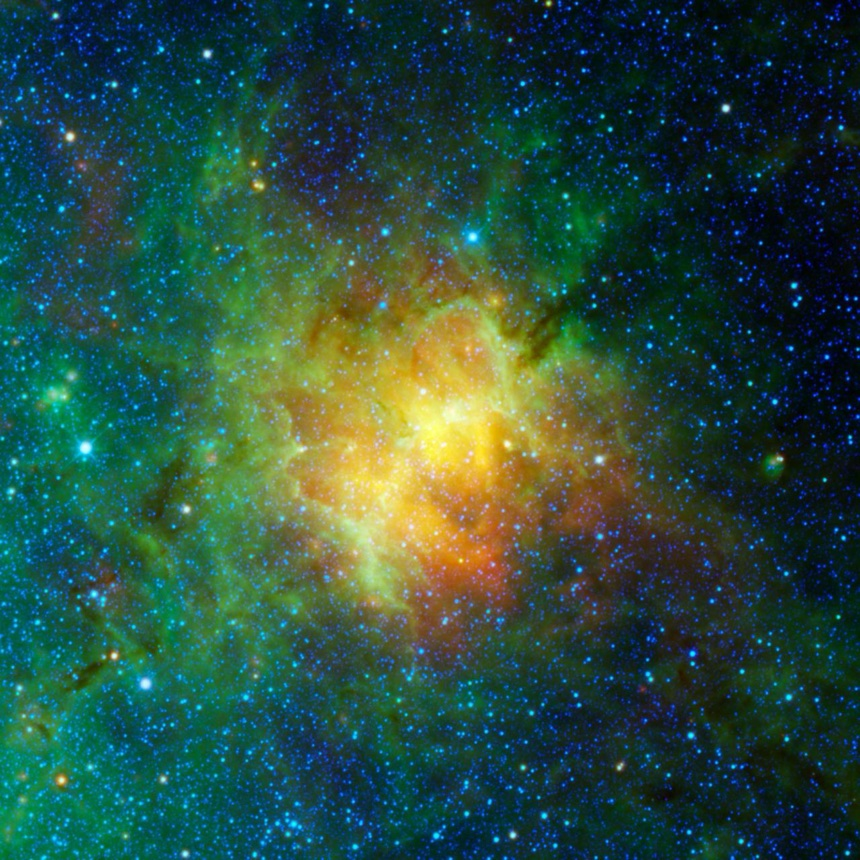
\includegraphics[width=0.78\textwidth,height=5.6cm,keepaspectratio]{../public/textures/nasa/pillars_of_creation.jpg}\\[3pt]
{\footnotesize\itshape\color{orbitarMuted} Fotografie reală NASA/ESA/CSA/STScI (Telescopul Spațial James Webb, PIA25433): \quotedblbase{}Stâlpii Creației\textquotedblright{} din Nebuloasa Vulturului (M16).}
\end{center}


\begin{tcolorbox}[orbitardata, title={\textbf{Repere esențiale: Stâlpii Creației (Nebuloasa Vulturului M16)}}]
\small
\begin{itemize}[leftmargin=1.4em, itemsep=2pt, topsep=2pt]
  \item \textbf{Clasificare și orbită:} Nebuloasă Cosmică \quad$\bullet$\quad \textbf{Distanță:} 6.500 de ani-lumină
  \item \textbf{Dimensiuni și masă:} Cel mai înalt stâlp are o lungime de aproximativ 4--5 ani-lumină, egală cu distanța de la Soarele nostru până la cea mai apropiată stea, Proxima Centauri! \quad$\bullet$\quad masă: 200000000,000 $\times M_\oplus$
  \item \textbf{Gravitație și regim termic:} 0,100 $\times g_\oplus$ (0,98 m/s$^2$) \quad$\bullet$\quad temperatură medie: +8.000 $^\circ$C
  \item \textbf{Ciclu orbital și rotație:} perioadă orbitală (an): Orbitează centrul Căii Lactee (aproximativ 230 de milioane de ani) \quad$\bullet$\quad rotație (zi): 24,00 ore (1,00 zile pământești)
  \item \textbf{Durata călătoriei de pe Pământ:} cu viteza luminii ($1c$): \emph{6.500 de ani}; cu racheta ($50.000$ de kilometri pe oră): \emph{117 milioane de ani}; cu avionul ($900$ de kilometri pe oră): \emph{8.100 de miliarde de ani}; cu mașina ($100$ de kilometri pe oră): \emph{73.000 de miliarde de ani}.
  \item \textbf{Repere de scară și curiozitate:} Stâlpii Creației seamănă cu trei munți de nori aurii ridicați în mijul cosmosului, atât de înalți încât o rază de lumină are nevoie de 5 ani întregi ca să urce de la baza unui stâlp până în vârful lui! Când Telescopul James Webb a privit Stâlpii Creației în lumină infraroșie, praful a devenit transparent și au apărut mii de stele tinere roșii ascunse chiar în interiorul coloanelor!
\end{itemize}
\end{tcolorbox}

\vspace{4pt}
\noindent\textbf{Prezentare generală și profil astrofizic.} Situați la aproximativ 6.500 de ani-lumină în Nebuloasa Vulturului (Messier 16, constelația Șarpele), Stâlpii Creației sunt trompe elefantine de hidrogen molecular rece și praf cosmic, sculptate prin fotoevaporare de vânturile stelare și radiația UV ale stelelor masive din roiul NGC 6611. Imaginile JWST (NIRCam și MIRI, 2022) au evidențiat protostele de clasă 0/I la extremitățile stâlpilor. Stâlpii Creației sunt trei turnuri uriașe de gaz și praf stelar din inima Nebuloasei Vulturului, devenite celebre în toată lumea datorită fotografiilor uimitoare realizate de telescoapele Hubble și James Webb! În vârful acestor coloane aurii și turcoaz, înalte de câțiva ani-lumină, se aprind stele noi-nouțe, roșii ca jarul! Stâlpii Creației seamănă cu trei munți de nori aurii ridicați în mijul cosmosului, atât de înalți încât o rază de lumină are nevoie de 5 ani întregi ca să urce de la baza unui stâlp până în vârful lui!

\medskip
\noindent\textbf{Scara cosmică și călătoria luminii în timp.} La scară astronomică, dimensiunile sale sunt impresionante: Cel mai înalt stâlp are o lungime de aproximativ 4--5 ani-lumină, egală cu distanța de la Soarele nostru până la cea mai apropiată stea, Proxima Centauri! Totodată, privind astăzi spre Stâlpii Creației (Nebuloasa Vulturului M16), observăm practic trecutul îndepărtat al Universului, întrucât lumina sa a călătorit prin spațiu până la noi: Lumina de la Stâlpii Creației pe care o vedem azi a plecat acum 6.500 de ani (în jurul anului 4500 î.Hr.), pe vremea străvechii culturi Cucuteni de pe teritoriul României!

\medskip
\noindent\textbf{Alcătuirea fizică și structura internă.} Privind în profunzimea sa, alcătuirea fizică este organizată pe mai multe straturi și regiuni distincte, fiecare având un rol bine definit în evoluția și dinamica acestui obiect cosmic. În primul rând se remarcă \textbf{Coloanele Moleculare (4--5 ani-lumină)}, trei piloni denși de hidrogen molecular și praf cosmic care protejează gazul din spate de radiația ultravioletă. În completarea acestui ansamblu întâlnim \textbf{Globule de Gaz în Evaporare (EGGs) \& Protostele}, noduri dense la vârful stâlpilor în care gravitația comprimă gazul, dând naștere unor stele tinere vizibile în infraroșu cu JWST.

\medskip
\noindent\textbf{Observații astronomice și istoricul explorării.} Fotografia iconică realizată de Telescopul Spațial Hubble în 1995 (și refăcută în 2014) a fost completată în octombrie 2022 de imaginea în infraroșu apropiat și mediu a Telescopului Spațial James Webb. Când Telescopul James Webb a privit Stâlpii Creației în lumină infraroșie, praful a devenit transparent și au apărut mii de stele tinere roșii ascunse chiar în interiorul coloanelor!

\vspace{6pt}
\begin{tcolorbox}[orbitarquiz, title={\textbf{Întrebare de verificare \#55: Stâlpii Creației (Nebuloasa Vulturului M16)}}]
\textbf{Ce a reușit să vadă Telescopul Spațial James Webb în interiorul Stâlpilor Creației folosind lumina infraroșie?}
\begin{itemize}[leftmargin=2.2em, itemsep=2pt, topsep=4pt]
  \item[$\square$ \textbf{A.}] A privit prin perdeaua de praf și a dezvăluit stelele tinere roșii care se nasc în vârful coloanelor
  \item[$\square$ \textbf{B.}] A descoperit un ocean de apă înghețată pe Marte
  \item[$\square$ \textbf{C.}] A fotografiat Stația Spațială Internațională
  \item[$\square$ \textbf{D.}] A măsurat coada unei comete din Centura Kuiper
\end{itemize}
\vspace{2pt}
{\footnotesize\color{orbitarMuted}\textbf{Răspuns corect:} \textbf{A} (A privit prin perdeaua de praf și a dezvăluit stelele tinere roșii care se nasc în vârful coloanelor). \emph{Lumina infraroșie pătrunde prin norii opaci de praf cosmic, permițând telescopului James Webb să fotografieze protostelele roșii nou-născute din interiorul Stâlpilor Creației.}}
\end{tcolorbox}
\clearpage


\section{Sagittarius A* (Gaura Neagră Supermasivă)}
\label{sec:body-sagittarius_a}
\vspace{-4pt}
{\large\itshape\color{orbitarAccent} Inima gravitațională din centrul Căii Lactee (26.000 ani-lumină)}\\[4pt]


\begin{center}
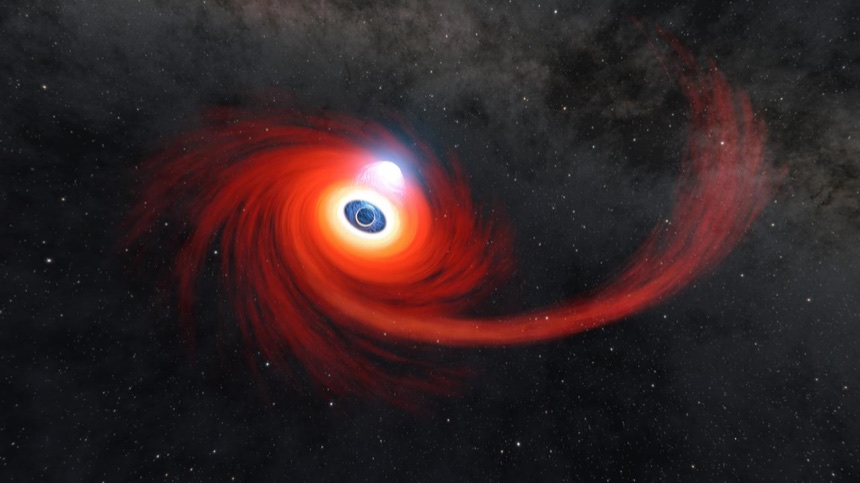
\includegraphics[width=0.78\textwidth,height=5.6cm,keepaspectratio]{../public/textures/nasa/sagittarius_a.jpg}\\[3pt]
{\footnotesize\itshape\color{orbitarMuted} Imaginea istorică reală Event Horizon Telescope (EHT) \& NASA (PIA25440): Gaura neagră supermasivă Sagittarius A* din centrul Căii Lactee.}
\end{center}


\begin{tcolorbox}[orbitardata, title={\textbf{Repere esențiale: Sagittarius A* (Gaura Neagră Supermasivă)}}]
\small
\begin{itemize}[leftmargin=1.4em, itemsep=2pt, topsep=2pt]
  \item \textbf{Clasificare și orbită:} Gaură Neagră Supermasivă \quad$\bullet$\quad \textbf{Distanță:} 26.000 de ani-lumină
  \item \textbf{Dimensiuni și masă:} Orizontul evenimentelor lui Sagittarius A* are diametrul de aproximativ 24 de milioane de kilometri (încape în interiorul orbitei lui Mercur), dar cântărește cât 4,3 milioane de Sori la un loc! \quad$\bullet$\quad masă: 1430000000000,000 $\times M_\oplus$
  \item \textbf{Gravitație și regim termic:} 1000000,000 $\times g_\oplus$ (9810000,00 m/s$^2$) \quad$\bullet$\quad temperatură medie: +1.000.000 $^\circ$C
  \item \textbf{Ciclu orbital și rotație:} perioadă orbitală (an): Orbitează centrul Căii Lactee (aproximativ 230 de milioane de ani) \quad$\bullet$\quad rotație (zi): 1,00 ore (0,04 zile pământești)
  \item \textbf{Durata călătoriei de pe Pământ:} cu viteza luminii ($1c$): \emph{26.000 de ani}; cu racheta ($50.000$ de kilometri pe oră): \emph{468 de milioane de ani}; cu avionul ($900$ de kilometri pe oră): \emph{32.000 de miliarde de ani}; cu mașina ($100$ de kilometri pe oră): \emph{290.000 de miliarde de ani}.
  \item \textbf{Repere de scară și curiozitate:} Sagittarius A* este ca \quotedblbase{}ancora gravitațională\textquotedblright{} din centrul unui carusel gigantic: se află la 26.000 de ani-lumină depărtare, în siguranță totală față de noi, iar întregul Sistem Solar se rotește liniștit în jurul centrului galaxiei o dată la 230 de milioane de ani! În anul 2022, astronomii au unit radiotelescoape de pe tot Pământul (Event Horizon Telescope) și au făcut prima fotografie reală din istorie a inelului portocaliu strălucitor din jurul lui Sagittarius A*!
\end{itemize}
\end{tcolorbox}

\vspace{4pt}
\noindent\textbf{Prezentare generală și profil astrofizic.} Sagittarius A* (Sgr A*), situată la aproximativ 26.000 de ani-lumină în direcția constelației Săgetătorul, este gaura neagră supermasivă din nucleul Căii Lactee. Are o masă de 4,3 milioane de mase solare și o rază Schwarzschild (orizontul evenimentelor, adică limita dincolo de care viteza de evadare depășește viteza luminii) de aproximativ 12 milioane de kilometri. Chiar în mijlocul galaxiei noastre, Calea Lactee, se află un obiect cosmic fascinant: Sagittarius A*, o gaură neagră supermasivă! Nu este o \quotedblbase{}gaură\textquotedblright{} goală, ci un loc în care masa a 4 milioane de Sori este adunată într-un spațiu mic. Gravitația ei este atât de puternică încât înconjoară întunericul central cu un inel luminos și fierbinte de gaz numit \quotedblbase{}disc de acreție\textquotedblright{}, iar lumina din spate este îndoită ca printr-o lupă! Sagittarius A* este ca \quotedblbase{}ancora gravitațională\textquotedblright{} din centrul unui carusel gigantic: se află la 26.000 de ani-lumină depărtare, în siguranță totală față de noi, iar întregul Sistem Solar se rotește liniștit în jurul centrului galaxiei o dată la 230 de milioane de ani!

\medskip
\noindent\textbf{Scara cosmică și călătoria luminii în timp.} La scară astronomică, dimensiunile sale sunt impresionante: Orizontul evenimentelor lui Sagittarius A* are diametrul de aproximativ 24 de milioane de kilometri (încape în interiorul orbitei lui Mercur), dar cântărește cât 4,3 milioane de Sori la un loc! Totodată, privind astăzi spre Sagittarius A* (Gaura Neagră Supermasivă), observăm practic trecutul îndepărtat al Universului, întrucât lumina sa a călătorit prin spațiu până la noi: Lumina discului din jurul găurii negre Sagittarius A* pe care o vedem azi a plecat acum 26.000 de ani, în timpul Epocii de Gheață, când oamenii preistorici pictau peșterile și pe Pământ trăiau mamuții!

\medskip
\noindent\textbf{Alcătuirea fizică și structura internă.} Privind în profunzimea sa, alcătuirea fizică este organizată pe mai multe straturi și regiuni distincte, fiecare având un rol bine definit în evoluția și dinamica acestui obiect cosmic. În primul rând se remarcă \textbf{Orizontul Evenimentelor (Raza Schwarzschild)}, frontiera sferică (aproximativ 12 milioane de kilometri rază) dincolo de care nici măcar fotonii de lumină nu mai pot scăpa de atracția gravitațională. În completarea acestui ansamblu întâlnim \textbf{Discul de Acreție \& Inelul Fotonic}, gaz ionizat rotindu-se la viteze relativiste în jurul găurii negre, a cărui lumină este curbată de lentila gravitațională.

\medskip
\noindent\textbf{Observații astronomice și istoricul explorării.} Existența ei a fost demonstrată prin urmărirea timp de 25 de ani a orbitelor stelelor \quotedblbase{}S\textquotedblright{} (în special steaua S2) de către Reinhard Genzel și Andrea Ghez (Premiul Nobel pentru Fizică 2020), iar în mai 2022 colaborarea Event Horizon Telescope (EHT) a publicat prima imagine directă a umbrei și a inelului său de acreție. În anul 2022, astronomii au unit radiotelescoape de pe tot Pământul (Event Horizon Telescope) și au făcut prima fotografie reală din istorie a inelului portocaliu strălucitor din jurul lui Sagittarius A*!

\vspace{6pt}
\begin{tcolorbox}[orbitarquiz, title={\textbf{Întrebare de verificare \#56: Sagittarius A* (Gaura Neagră Supermasivă)}}]
\textbf{Ce este \quotedblbase{}orizontul evenimentelor\textquotedblright{} al găurii negre Sagittarius A* din centrul Căii Lactee?}
\begin{itemize}[leftmargin=2.2em, itemsep=2pt, topsep=4pt]
  \item[$\square$ \textbf{A.}] Limita în jurul găurii negre dincolo de care gravitația este atât de puternică încât nici lumina nu mai poate ieși
  \item[$\square$ \textbf{B.}] Un lanț de munți de pe planeta Marte
  \item[$\square$ \textbf{C.}] Numele unei sonde spațiale lansate spre Jupiter
  \item[$\square$ \textbf{D.}] Un strat de nori din atmosfera Pământului
\end{itemize}
\vspace{2pt}
{\footnotesize\color{orbitarMuted}\textbf{Răspuns corect:} \textbf{A} (Limita în jurul găurii negre dincolo de care gravitația este atât de puternică încât nici lumina nu mai poate ieși). \emph{Orizontul evenimentelor este granița gravitațională a unei găuri negre unde viteza necesară pentru a scăpa depășește viteza luminii (300.000 kilometri pe secundă).}}
\end{tcolorbox}
\clearpage


\section{Calea Lactee (Galaxia Noastră)}
\label{sec:body-milky_way}
\vspace{-4pt}
{\large\itshape\color{orbitarAccent} Galaxia noastră spirală cu aproximativ 200--400 de miliarde de stele; Soarele se află în Brațul Orion (la 26.000 a.l. de centru)}\\[4pt]


\begin{center}
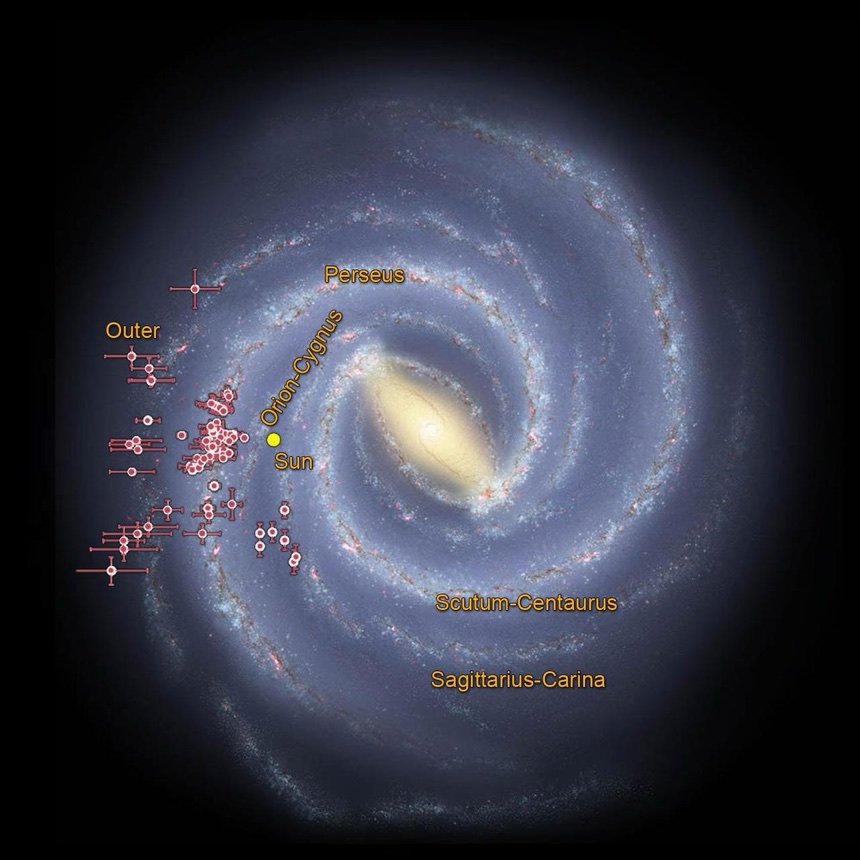
\includegraphics[width=0.78\textwidth,height=5.6cm,keepaspectratio]{../public/textures/nasa/milky_way.jpg}\\[3pt]
{\footnotesize\itshape\color{orbitarMuted} Harta științifică oficială NASA/JPL-Caltech (Telescopul Spitzer PIA19341): Brațele spirale ale galaxiei noastre, Calea Lactee, și poziția Soarelui.}
\end{center}


\begin{tcolorbox}[orbitardata, title={\textbf{Repere esențiale: Calea Lactee (Galaxia Noastră)}}]
\small
\begin{itemize}[leftmargin=1.4em, itemsep=2pt, topsep=2pt]
  \item \textbf{Clasificare și orbită:} Galaxie \quad$\bullet$\quad \textbf{Distanță:} Diametru aproximativ 100.000 ani-lumină (Soarele la 26.000 a.l. de centru)
  \item \textbf{Dimensiuni și masă:} Calea Lactee are un diametru de aproximativ 100.000 de ani-lumină și adăpostește între 200 și 400 de miliarde de stele! Sistemul nostru Solar este doar un punct minuscul în Brațul Orion, la jumătatea distanței dintre centru și margine! \quad$\bullet$\quad masă: 333000000000000000,000 $\times M_\oplus$
  \item \textbf{Gravitație și regim termic:} 1,000 $\times g_\oplus$ (9,81 m/s$^2$) \quad$\bullet$\quad temperatură medie: -270 $^\circ$C
  \item \textbf{Ciclu orbital și rotație:} perioadă orbitală (an): 83.950.000.000 zile ($\approx$ 229842573,58 ani pământești) \quad$\bullet$\quad rotație (zi): 24,00 ore (1,00 zile pământești)
  \item \textbf{Durata călătoriei de pe Pământ:} cu viteza luminii ($1c$): \emph{100.000 de ani (diametrul galaxiei)}; cu racheta ($50.000$ de kilometri pe oră): \emph{1,8 miliarde de ani}; cu avionul ($900$ de kilometri pe oră): \emph{120.000 de miliarde de ani}; cu mașina ($100$ de kilometri pe oră): \emph{1.100.000 de miliarde de ani (de la un capăt la altul)}.
  \item \textbf{Repere de scară și curiozitate:} Dacă întreaga Cale Lactee ar fi cât un stadion mare de fotbal, tot Sistemul nostru Solar (cu Soarele și toate cele 8 planete) ar fi mai mic decât un singur fir de praf așezat pe iarbă, la jumătatea distanței dintre centrul terenului și tribună! Soarele și Pământul călătoresc prin galaxie cu 828.000 kilometri pe oră, dar Calea Lactee este atât de mare încât ne trebuie 230 de milioane de ani ca să facem un singur tur complet (numit \quotedblbase{}un an galactic\textquotedblright{}), astfel că ultima dată când Sistemul Solar s-a aflat în același loc pe orbită, primii dinozauri abia apăreau pe Pământ!
\end{itemize}
\end{tcolorbox}

\vspace{4pt}
\noindent\textbf{Prezentare generală și profil astrofizic.} Calea Lactee este o galaxie spirală barată (tip morfologic SBbc) cu diametrul discului stelar de aproximativ 100.000 de ani-lumină, grosimea de aproximativ 1.000 de ani-lumină și o populație de 200--400 de miliarde de stele. Sistemul Solar este situat în Brațul Local (Orion-Cygnus), la aproximativ 26.000 de ani-lumină de nucleul galactic (Sagittarius A*), orbitând cu aproximativ 220--230 kilometri pe secundă. Calea Lactee este marea noastră casă din Univers, un imens disc cosmic în formă de morișcă spiralată, format din peste 200 de miliarde de stele! Soarele nostru, împreună cu Pământul și toate planetele, locuiește într-un cartier liniștit numit \quotedblbase{}Brațul Orion\textquotedblright{}, la 26.000 de ani-lumină de centrul luminos al galaxiei! Dacă întreaga Cale Lactee ar fi cât un stadion mare de fotbal, tot Sistemul nostru Solar (cu Soarele și toate cele 8 planete) ar fi mai mic decât un singur fir de praf așezat pe iarbă, la jumătatea distanței dintre centrul terenului și tribună!

\medskip
\noindent\textbf{Scara cosmică și călătoria luminii în timp.} La scară astronomică, dimensiunile sale sunt impresionante: Calea Lactee are un diametru de aproximativ 100.000 de ani-lumină și adăpostește între 200 și 400 de miliarde de stele! Sistemul nostru Solar este doar un punct minuscul în Brațul Orion, la jumătatea distanței dintre centru și margine! Totodată, privind astăzi spre Calea Lactee (Galaxia Noastră), observăm practic trecutul îndepărtat al Universului, întrucât lumina sa a călătorit prin spațiu până la noi: Lumina îi ia 100.000 de ani ca să traverseze Calea Lactee de la o margine la cealaltă, iar de la centrul galaxiei până la Pământ călătorește 26.000 de ani!

\medskip
\noindent\textbf{Alcătuirea fizică și structura internă.} Privind în profunzimea sa, alcătuirea fizică este organizată pe mai multe straturi și regiuni distincte, fiecare având un rol bine definit în evoluția și dinamica acestui obiect cosmic. În primul rând se remarcă \textbf{Nucleul Galactic \& Bara Centrală}, regiune centrală densă de stele bătrâne galben-aurii în jurul găurii negre supermasive Sagittarius A*. În strânsă legătură cu această componentă se află \textbf{Brațele Spirale (Perseu, Scutum-Centaurus, Sagittarius, Norma)}, brațe bogate în gaz interstelar, nebuloase și stele tinere albastre fierbinți. În completarea acestui ansamblu întâlnim \textbf{Brațul Orion, Casa Sistemului Solar}, brațul spiral secundar aflat la 26.000 de ani-lumină de centru, unde se găsesc Soarele, Nebuloasa Orion și Pleiadele.

\medskip
\noindent\textbf{Observații astronomice și istoricul explorării.} În 1610, Galileo Galilei a demonstrat cu luneta sa că banda lăptoasă de pe cer este compusă din nenumărate stele; în anii 1920, Harlow Shapley și Edwin Hubble au stabilit dimensiunile galaxiei noastre și existența altor galaxii, iar misiunea europeană Gaia (ESA) a cartografiat recent în 3D aproape 2 miliarde de stele din Calea Lactee. Soarele și Pământul călătoresc prin galaxie cu 828.000 kilometri pe oră, dar Calea Lactee este atât de mare încât ne trebuie 230 de milioane de ani ca să facem un singur tur complet (numit \quotedblbase{}un an galactic\textquotedblright{}), astfel că ultima dată când Sistemul Solar s-a aflat în același loc pe orbită, primii dinozauri abia apăreau pe Pământ!

\vspace{6pt}
\begin{tcolorbox}[orbitarquiz, title={\textbf{Întrebare de verificare \#57: Calea Lactee (Galaxia Noastră)}}]
\textbf{Unde se află Sistemul nostru Solar în cadrul Galaxiei Calea Lactee?}
\begin{itemize}[leftmargin=2.2em, itemsep=2pt, topsep=4pt]
  \item[$\square$ \textbf{A.}] În Brațul Orion, la aproximativ 26.000 de ani-lumină de centrul galaxiei
  \item[$\square$ \textbf{B.}] Chiar în mijlocul găurii negre centrale
  \item[$\square$ \textbf{C.}] În afara galaxiei, lângă Andromeda
  \item[$\square$ \textbf{D.}] Pe suprafața stelei Betelgeuse
\end{itemize}
\vspace{2pt}
{\footnotesize\color{orbitarMuted}\textbf{Răspuns corect:} \textbf{A} (În Brațul Orion, la aproximativ 26.000 de ani-lumină de centrul galaxiei). \emph{Soarele și planetele noastre se află în Brațul Orion, la aproximativ 26.000 de ani-lumină de centrul Căii Lactee (cam la jumătatea razei discului galactic).}}
\end{tcolorbox}
\clearpage


\section{Galaxia Andromeda (M31)}
\label{sec:body-andromeda}
\vspace{-4pt}
{\large\itshape\color{orbitarAccent} Cea mai apropiată galaxie spirală mare, cu aproximativ 1.000 de miliarde de stele (2,5 milioane ani-lumină)}\\[4pt]


\begin{center}
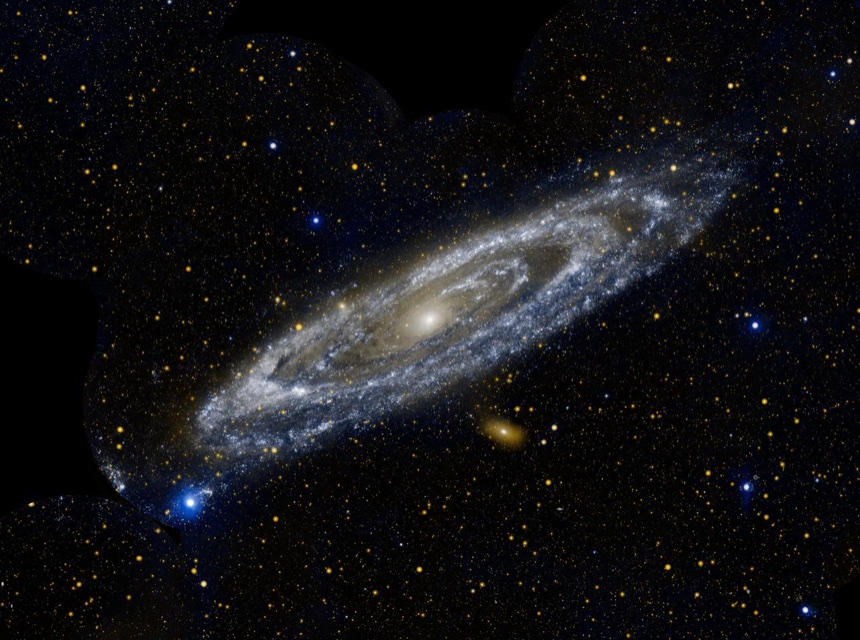
\includegraphics[width=0.78\textwidth,height=5.6cm,keepaspectratio]{../public/textures/nasa/andromeda.jpg}\\[3pt]
{\footnotesize\itshape\color{orbitarMuted} Fotografie reală NASA/JPL-Caltech (GALEX \& Spitzer PIA15416): Galaxia spirală Andromeda (M31), aflată la 2,54 de milioane de ani-lumină.}
\end{center}


\begin{tcolorbox}[orbitardata, title={\textbf{Repere esențiale: Galaxia Andromeda (M31)}}]
\small
\begin{itemize}[leftmargin=1.4em, itemsep=2pt, topsep=2pt]
  \item \textbf{Clasificare și orbită:} Galaxie \quad$\bullet$\quad \textbf{Distanță:} 2,54 de milioane de ani-lumină
  \item \textbf{Dimensiuni și masă:} Galaxia Andromeda are un diametru de aproximativ 150.000--220.000 de ani-lumină și aproximativ 1.000 de miliarde (un bilion) de stele și este chiar mai mare decât Calea Lactee! \quad$\bullet$\quad masă: 500000000000000000,000 $\times M_\oplus$
  \item \textbf{Gravitație și regim termic:} 1,000 $\times g_\oplus$ (9,81 m/s$^2$) \quad$\bullet$\quad temperatură medie: -270 $^\circ$C
  \item \textbf{Ciclu orbital și rotație:} perioadă orbitală (an): Orbitează centrul Căii Lactee (aproximativ 230 de milioane de ani) \quad$\bullet$\quad rotație (zi): 24,00 ore (1,00 zile pământești)
  \item \textbf{Durata călătoriei de pe Pământ:} cu viteza luminii ($1c$): \emph{2,54 de milioane de ani}; cu racheta ($50.000$ de kilometri pe oră): \emph{45 de miliarde de ani}; cu avionul ($900$ de kilometri pe oră): \emph{3,1 milioane de miliarde de ani}; cu mașina ($100$ de kilometri pe oră): \emph{28 de milioane de miliarde de ani}.
  \item \textbf{Repere de scară și curiozitate:} Dacă Calea Lactee ar fi o farfurie mare pe masă, Galaxia Andromeda ar fi o farfurie și mai mare aflată la doar câțiva metri distanță, iar lumina de la ea călătorește spre noi timp de 2,5 milioane de ani! Calea Lactee și Galaxia Andromeda se apropie una de cealaltă cu 400.000 kilometri pe oră! Peste aproximativ 4,5 miliarde de ani, cele două galaxii vor dansa împreună și se vor uni într-o singură galaxie gigantă fără ca stelele să se ciocnească între ele!
\end{itemize}
\end{tcolorbox}

\vspace{4pt}
\noindent\textbf{Prezentare generală și profil astrofizic.} Galaxia Andromeda (Messier 31 / NGC 224), aflată la 2,537 de milioane de ani-lumină în constelația Andromeda, este cea mai mare galaxie din Grupul Local (care include și Calea Lactee și Galaxia Triunghiului M33). Cu un diametru de aproximativ 152.000--220.000 de ani-lumină și aproximativ 10$^1$$^2$ stele, Andromeda a jucat un rol decisiv în istoria științei când Edwin Hubble a demonstrat în 1924 că este o \quotedblbase{}insulă-univers\textquotedblright{} separată de Calea Lactee. Galaxia Andromeda (M31) este \quotedblbase{}sora mai mare\textquotedblright{} a Căii Lactee și cel mai îndepărtat obiect din Univers pe care îl poți vedea cu ochiul liber, fără telescop, într-o noapte senină la munte! Este o galaxie spirală uriașă cu o mie de miliarde de stele, aflată la 2,5 milioane de ani-lumină de noi! Dacă Calea Lactee ar fi o farfurie mare pe masă, Galaxia Andromeda ar fi o farfurie și mai mare aflată la doar câțiva metri distanță, iar lumina de la ea călătorește spre noi timp de 2,5 milioane de ani!

\medskip
\noindent\textbf{Scara cosmică și călătoria luminii în timp.} La scară astronomică, dimensiunile sale sunt impresionante: Galaxia Andromeda are un diametru de aproximativ 150.000--220.000 de ani-lumină și aproximativ 1.000 de miliarde (un bilion) de stele și este chiar mai mare decât Calea Lactee! Totodată, privind astăzi spre Galaxia Andromeda (M31), observăm practic trecutul îndepărtat al Universului, întrucât lumina sa a călătorit prin spațiu până la noi: Lumina de la Galaxia Andromeda pe care o vedem azi cu ochiul liber într-o noapte senină la munte a plecat acum 2,5 milioane de ani, de la începutul Cuaternarului, cu mult înainte să apară omul modern (Homo sapiens) pe Pământ!

\medskip
\noindent\textbf{Alcătuirea fizică și structura internă.} Privind în profunzimea sa, alcătuirea fizică este organizată pe mai multe straturi și regiuni distincte, fiecare având un rol bine definit în evoluția și dinamica acestui obiect cosmic. În primul rând se remarcă \textbf{Nucleu Dublu \& Gaură Neagră de aproximativ 100 Milioane M$_\odot$}, centru galactic masiv observat de telescopul Hubble, multă vreme mai masiv decât nucleul Căii Lactee. În completarea acestui ansamblu întâlnim \textbf{Discul Spiral și Galaxiile Satelit (M32 \& M110)}, brațe spirale bogate în roiuri stelare și praf, însoțite de galaxiile pitice eliptice M32 și M110.

\medskip
\noindent\textbf{Observații astronomice și istoricul explorării.} Menționată în anul 964 de astronomul persan Abd al-Rahman al-Sufi drept \quotedblbase{}un mic nor\textquotedblright{}; în 1924, Edwin Hubble a identificat stele variabile Cefeide în M31, demonstrând că Universul se întinde mult dincolo de Calea Lactee. Calea Lactee și Galaxia Andromeda se apropie una de cealaltă cu 400.000 kilometri pe oră! Peste aproximativ 4,5 miliarde de ani, cele două galaxii vor dansa împreună și se vor uni într-o singură galaxie gigantă fără ca stelele să se ciocnească între ele!

\vspace{6pt}
\begin{tcolorbox}[orbitarquiz, title={\textbf{Întrebare de verificare \#58: Galaxia Andromeda (M31)}}]
\textbf{Care este cel mai îndepărtat obiect cosmic vizibil cu ochiul liber pe cerul nopții și la ce distanță se află?}
\begin{itemize}[leftmargin=2.2em, itemsep=2pt, topsep=4pt]
  \item[$\square$ \textbf{A.}] Galaxia Andromeda (M31), aflată la aproximativ 2,5 milioane de ani-lumină
  \item[$\square$ \textbf{B.}] Planeta Neptun, la 4 ore-lumină
  \item[$\square$ \textbf{C.}] Luna, la 1,3 secunde-lumină
  \item[$\square$ \textbf{D.}] Sonda Voyager 1, la 22 ore-lumină
\end{itemize}
\vspace{2pt}
{\footnotesize\color{orbitarMuted}\textbf{Răspuns corect:} \textbf{A} (Galaxia Andromeda (M31), aflată la aproximativ 2,5 milioane de ani-lumină). \emph{Galaxia Andromeda (M31), situată la 2,54 de milioane de ani-lumină, poate fi văzută cu ochiul liber într-o noapte fără poluare luminoasă.}}
\end{tcolorbox}
\clearpage


\section{Nebuloasa Carina (\quotedblbase{}Stâncile Cosmice\textquotedblright{}, NGC 3372)}
\label{sec:body-carina_nebula}
\vspace{-4pt}
{\large\itshape\color{orbitarAccent} Una dintre cele mai mari maternități de stele din Calea Lactee, fotografiată de James Webb (7.500 ani-lumină)}\\[4pt]



\begin{tcolorbox}[orbitardata, title={\textbf{Repere esențiale: Nebuloasa Carina (\quotedblbase{}Stâncile Cosmice\textquotedblright{}, NGC 3372)}}]
\small
\begin{itemize}[leftmargin=1.4em, itemsep=2pt, topsep=2pt]
  \item \textbf{Clasificare și orbită:} Nebuloasă Cosmică \quad$\bullet$\quad \textbf{Distanță:} 7.500 de ani-lumină
  \item \textbf{Dimensiuni și masă:} Nebuloasa Carina se întinde pe aproximativ 300 de ani-lumină și este de peste 10 ori mai mare decât Nebuloasa Orion! \quad$\bullet$\quad masă: 300000000,000 $\times M_\oplus$
  \item \textbf{Gravitație și regim termic:} 0,100 $\times g_\oplus$ (0,98 m/s$^2$) \quad$\bullet$\quad temperatură medie: +9.500 $^\circ$C
  \item \textbf{Ciclu orbital și rotație:} perioadă orbitală (an): Orbitează centrul Căii Lactee (aproximativ 230 de milioane de ani) \quad$\bullet$\quad rotație (zi): 24,00 ore (1,00 zile pământești)
  \item \textbf{Durata călătoriei de pe Pământ:} cu viteza luminii ($1c$): \emph{7.500 de ani}; cu racheta ($50.000$ de kilometri pe oră): \emph{135 de milioane de ani}; cu avionul ($900$ de kilometri pe oră): \emph{9.300 de miliarde de ani}; cu mașina ($100$ de kilometri pe oră): \emph{84.000 de miliarde de ani}.
  \item \textbf{Repere de scară și curiozitate:} Nebuloasa Carina arată ca un lanț muntos de chihlimbar scăldat de un cer azuriu, doar că \quotedblbase{}munții\textquotedblright{} sunt făcuți din nori de praf stelar mai înalți decât distanța de la Soare la cea mai apropiată stea! În inima Nebuloasei Carina locuiește Eta Carinae, un sistem de două stele monstruoase care luminează cât 5 milioane de Sori la un loc!
\end{itemize}
\end{tcolorbox}

\vspace{4pt}
\noindent\textbf{Prezentare generală și profil astrofizic.} Nebuloasa Carina (NGC 3372), situată la aproximativ 7.500 de ani-lumină în Brațul Carina-Sagittarius al Căii Lactee, este una dintre cele mai întinse regiuni H II din galaxia noastră (aproximativ 300 ani-lumină diametru). Pe marginea cavității NGC 3324 se ridică \quotedblbase{}Stâncile Cosmice\textquotedblright{}, sculptate de vânturile stelare și radiația ultravioletă a stelelor masive tinere de tip O. Nebuloasa Carina este un ținut cosmic uriaș, unde munți înalți de gaz și praf portocaliu se întâlnesc cu o mare strălucitoare de lumină albastră! Prima fotografie celebră trimisă de Telescopul Spațial James Webb ne-a arătat aici \quotedblbase{}Stâncile Cosmice\textquotedblright{}, creste înalte de 7 ani-lumină în care se aprind mii de stele noi! Nebuloasa Carina arată ca un lanț muntos de chihlimbar scăldat de un cer azuriu, doar că \quotedblbase{}munții\textquotedblright{} sunt făcuți din nori de praf stelar mai înalți decât distanța de la Soare la cea mai apropiată stea!

\medskip
\noindent\textbf{Scara cosmică și călătoria luminii în timp.} La scară astronomică, dimensiunile sale sunt impresionante: Nebuloasa Carina se întinde pe aproximativ 300 de ani-lumină și este de peste 10 ori mai mare decât Nebuloasa Orion! Totodată, privind astăzi spre Nebuloasa Carina (\quotedblbase{}Stâncile Cosmice\textquotedblright{}, NGC 3372), observăm practic trecutul îndepărtat al Universului, întrucât lumina sa a călătorit prin spațiu până la noi: Lumina de la Stâncile Cosmice din Nebuloasa Carina a plecat spre Pământ acum 7.500 de ani (în jurul anului 5500 î.Hr.), la începutul Neoliticului!

\medskip
\noindent\textbf{Alcătuirea fizică și structura internă.} Privind în profunzimea sa, alcătuirea fizică este organizată pe mai multe straturi și regiuni distincte, fiecare având un rol bine definit în evoluția și dinamica acestui obiect cosmic. În primul rând se remarcă \textbf{Stâncile Cosmice (NGC 3324)}, front de gaz și praf înalt de aproximativ 7 ani-lumină, modelat de radiația ionizantă și străbătut de jeturi protostelare. În completarea acestui ansamblu întâlnim \textbf{Sistemul Hipergigant Eta Carinae \& Nebuloasa Homunculus}, stea variabilă luminoasă albastră (aproximativ 100 mase solare) înconjurată de doi lobi bipolari de gaz expulzați în Marea Erupție din 1843.

\medskip
\noindent\textbf{Observații astronomice și istoricul explorării.} Descoperită în 1752 de Nicolas-Louis de Lacaille de la Capul Bunei Speranțe; în iulie 2022, \quotedblbase{}Stâncile Cosmice\textquotedblright{} au devenit una dintre primele imagini istorice publicate de Telescopul Spațial James Webb. În inima Nebuloasei Carina locuiește Eta Carinae, un sistem de două stele monstruoase care luminează cât 5 milioane de Sori la un loc!

\vspace{6pt}
\begin{tcolorbox}[orbitarquiz, title={\textbf{Întrebare de verificare \#59: Nebuloasa Carina (\quotedblbase{}Stâncile Cosmice\textquotedblright{}, NGC 3372)}}]
\textbf{Cum se numește formațiunea spectaculoasă din Nebuloasa Carina fotografiată în prima serie de imagini a Telescopului James Webb?}
\begin{itemize}[leftmargin=2.2em, itemsep=2pt, topsep=4pt]
  \item[$\square$ \textbf{A.}] Stâncile Cosmice, creste de gaz și praf înalte de 7 ani-lumină unde se nasc stele
  \item[$\square$ \textbf{B.}] Inelul lui Saturn
  \item[$\square$ \textbf{C.}] Craterul Tycho de pe Lună
  \item[$\square$ \textbf{D.}] Marea Pată Roșie de pe Jupiter
\end{itemize}
\vspace{2pt}
{\footnotesize\color{orbitarMuted}\textbf{Răspuns corect:} \textbf{A} (Stâncile Cosmice, creste de gaz și praf înalte de 7 ani-lumină unde se nasc stele). \emph{\quotedblbase{}Stâncile Cosmice\textquotedblright{} din NGC 3324 (Nebuloasa Carina) reprezintă marginea unei cavități gazoase uriașe sculptate de stele tinere masive.}}
\end{tcolorbox}
\clearpage


\section{Nebuloasa Crabului (M1)}
\label{sec:body-crab_nebula}
\vspace{-4pt}
{\large\itshape\color{orbitarAccent} Rămășița luminoasă a supernovei observate în anul 1054, cu un pulsar în centru (6.500 ani-lumină)}\\[4pt]



\begin{tcolorbox}[orbitardata, title={\textbf{Repere esențiale: Nebuloasa Crabului (M1)}}]
\small
\begin{itemize}[leftmargin=1.4em, itemsep=2pt, topsep=2pt]
  \item \textbf{Clasificare și orbită:} Nebuloasă Cosmică \quad$\bullet$\quad \textbf{Distanță:} 6.500 de ani-lumină
  \item \textbf{Dimensiuni și masă:} Nebuloasa Crabului are un diametru de 11 ani-lumină și încă se mărește în fiecare secundă cu 1.500 kilometri pe secundă! \quad$\bullet$\quad masă: 1500000,000 $\times M_\oplus$
  \item \textbf{Gravitație și regim termic:} 1,000 $\times g_\oplus$ (9,81 m/s$^2$) \quad$\bullet$\quad temperatură medie: +15.000 $^\circ$C
  \item \textbf{Ciclu orbital și rotație:} perioadă orbitală (an): Orbitează centrul Căii Lactee (aproximativ 230 de milioane de ani) \quad$\bullet$\quad rotație (zi): 0,00 ore (0,00 zile pământești)
  \item \textbf{Durata călătoriei de pe Pământ:} cu viteza luminii ($1c$): \emph{6.500 de ani}; cu racheta ($50.000$ de kilometri pe oră): \emph{117 milioane de ani}; cu avionul ($900$ de kilometri pe oră): \emph{8.100 de miliarde de ani}; cu mașina ($100$ de kilometri pe oră): \emph{73.000 de miliarde de ani}.
  \item \textbf{Repere de scară și curiozitate:} În mijlocul Nebuloasei Crabului se află \quotedblbase{}inima\textquotedblright{} stelei care a explodat: o stea neutronică mică doar cât un oraș (25 de kilometri), dar care se învârte ca un titirez de 30 de ori pe secundă și trimite fascicule de lumină ca un far cosmic! Nebuloasa Crabului este primul obiect trecut în faimosul catalog al astronomului Charles Messier, motiv pentru care poartă numele \quotedblbase{}M1\textquotedblright{} (Messier 1)!
\end{itemize}
\end{tcolorbox}

\vspace{4pt}
\noindent\textbf{Prezentare generală și profil astrofizic.} Nebuloasa Crabului (Messier 1 / NGC 1952), situată la 6.500 de ani-lumină în constelația Taurul, este o rămășiță de supernovă și o nebuloasă de vânt pulsaric alimentată de Pulsarul din Crab (PSR B0531+21). Steaua neutronică centrală se rotește la fiecare 33 de milisecunde (aproximativ 30 rotații pe secundă), accelerând electroni la viteze relativiste care emit radiație sincrotron albăstruie. În anul 1054, oamenii de pe Pământ au văzut pe cer o \quotedblbase{}stea nouă\textquotedblright{} atât de strălucitoare încât se vedea chiar și ziua, în plin soare! Era explozia unei stele uriașe (o supernovă), iar norul țesut din filamente colorate rămas în urma ei se numește azi Nebuloasa Crabului! În mijlocul Nebuloasei Crabului se află \quotedblbase{}inima\textquotedblright{} stelei care a explodat: o stea neutronică mică doar cât un oraș (25 de kilometri), dar care se învârte ca un titirez de 30 de ori pe secundă și trimite fascicule de lumină ca un far cosmic!

\medskip
\noindent\textbf{Scara cosmică și călătoria luminii în timp.} La scară astronomică, dimensiunile sale sunt impresionante: Nebuloasa Crabului are un diametru de 11 ani-lumină și încă se mărește în fiecare secundă cu 1.500 kilometri pe secundă! Totodată, privind astăzi spre Nebuloasa Crabului (M1), observăm practic trecutul îndepărtat al Universului, întrucât lumina sa a călătorit prin spațiu până la noi: Explozia stelei a fost văzută pe cerul Pământului în anul 1054 d.Hr., dar lumina acelei explozii plecase din Nebuloasa Crabului cu 6.500 de ani mai devreme!

\medskip
\noindent\textbf{Alcătuirea fizică și structura internă.} Privind în profunzimea sa, alcătuirea fizică este organizată pe mai multe straturi și regiuni distincte, fiecare având un rol bine definit în evoluția și dinamica acestui obiect cosmic. În primul rând se remarcă \textbf{Pulsarul din Crab (Stea Neutronică)}, nucleu stelar colapsat cu diametrul de aproximativ 25 de kilometri și masa de 1,4 Sori, care se rotește de 30 de ori pe secundă. În completarea acestui ansamblu întâlnim \textbf{Cușca de Filamente și Nebuloasa Sincrotron}, rețea tridimensională de filamente bogate în heliu, carbon, oxigen și sulf ce se extinde cu aproximativ 1.500 kilometri pe secundă.

\medskip
\noindent\textbf{Observații astronomice și istoricul explorării.} Supernova SN 1054 a fost consemnată de astronomii chinezi și arabi în iulie 1054; nebuloasa a fost redescoperită în 1731 de John Bevis și catalogată drept M1 de Charles Messier în 1758. Nebuloasa Crabului este primul obiect trecut în faimosul catalog al astronomului Charles Messier, motiv pentru care poartă numele \quotedblbase{}M1\textquotedblright{} (Messier 1)!

\vspace{6pt}
\begin{tcolorbox}[orbitarquiz, title={\textbf{Întrebare de verificare \#60: Nebuloasa Crabului (M1)}}]
\textbf{Ce obiect extraordinar se află chiar în centrul Nebuloasei Crabului (M1)?}
\begin{itemize}[leftmargin=2.2em, itemsep=2pt, topsep=4pt]
  \item[$\square$ \textbf{A.}] Un pulsar (o stea neutronică densă cât un oraș) care se rotește de 30 de ori pe secundă
  \item[$\square$ \textbf{B.}] O planetă acoperită cu păduri tropicale
  \item[$\square$ \textbf{C.}] Un satelit natural al planetei Neptun
  \item[$\square$ \textbf{D.}] O cometă de gheață din Norul lui Oort
\end{itemize}
\vspace{2pt}
{\footnotesize\color{orbitarMuted}\textbf{Răspuns corect:} \textbf{A} (Un pulsar (o stea neutronică densă cât un oraș) care se rotește de 30 de ori pe secundă). \emph{În centrul Nebuloasei Crabului se află Pulsarul din Crab, o stea neutronică rămasă după supernova din anul 1054.}}
\end{tcolorbox}
\clearpage


\section{Nebuloasa Inelul (M57)}
\label{sec:body-ring_nebula}
\vspace{-4pt}
{\large\itshape\color{orbitarAccent} Inelul cosmic în culorile curcubeului lăsat în urmă de o stea asemănătoare Soarelui (2.300 ani-lumină)}\\[4pt]



\begin{tcolorbox}[orbitardata, title={\textbf{Repere esențiale: Nebuloasa Inelul (M57)}}]
\small
\begin{itemize}[leftmargin=1.4em, itemsep=2pt, topsep=2pt]
  \item \textbf{Clasificare și orbită:} Nebuloasă Cosmică \quad$\bullet$\quad \textbf{Distanță:} 2.300 de ani-lumină
  \item \textbf{Dimensiuni și masă:} Inelul luminos principal are un diametru de aproximativ 1,3 ani-lumină, fiind de peste 400 de ori mai lat decât orbita planetei Neptun în jurul Soarelui! \quad$\bullet$\quad masă: 200000,000 $\times M_\oplus$
  \item \textbf{Gravitație și regim termic:} 0,500 $\times g_\oplus$ (4,91 m/s$^2$) \quad$\bullet$\quad temperatură medie: +100.000 $^\circ$C
  \item \textbf{Ciclu orbital și rotație:} perioadă orbitală (an): Orbitează centrul Căii Lactee (aproximativ 230 de milioane de ani) \quad$\bullet$\quad rotație (zi): 24,00 ore (1,00 zile pământești)
  \item \textbf{Durata călătoriei de pe Pământ:} cu viteza luminii ($1c$): \emph{2.300 de ani}; cu racheta ($50.000$ de kilometri pe oră): \emph{41 de milioane de ani}; cu avionul ($900$ de kilometri pe oră): \emph{2.850 de miliarde de ani}; cu mașina ($100$ de kilometri pe oră): \emph{26.000 de miliarde de ani}.
  \item \textbf{Repere de scară și curiozitate:} În mijlocul inelului colorat se vede un punctuleț alb ca o perlă: este o \quotedblbase{}pitică albă\textquotedblright{}, adică miezul cald al stelei, de mărimea Pământului, care luminează gazul din jur ca o lampă cosmică! Telescopul James Webb a descoperit că în jurul inelului se află 20.000 de globuri dense de gaz și zece arce concentrice, ca valurile lăsate de o pietricică într-un lac!
\end{itemize}
\end{tcolorbox}

\vspace{4pt}
\noindent\textbf{Prezentare generală și profil astrofizic.} Nebuloasa Inelul (Messier 57 / NGC 6720), aflată la aproximativ 2.300 de ani-lumină în constelația Lira, este o nebuloasă planetară arhetipală. Deși văzută dinspre Pământ pare un inel, observațiile Hubble și JWST arată că are forma unui cilindru/butoi de gaz ionizat văzut aproape de-a lungul axei polare, iluminat de o pitică albă centrală cu temperatura de aproximativ 120.000 $^\circ$C. Nebuloasa Inelul (M57) arată ca o gogoașă sau un inel fermecat în culorile curcubeului care plutește în spațiu: albastru în interior, verde-turcoaz la mijloc și roșu-auriu pe margine! Ea nu s-a format dintr-o explozie violentă, ci atunci când o stea bătrână, asemănătoare Soarelui nostru, și-a suflat ușor straturile exterioare în spațiu! În mijlocul inelului colorat se vede un punctuleț alb ca o perlă: este o \quotedblbase{}pitică albă\textquotedblright{}, adică miezul cald al stelei, de mărimea Pământului, care luminează gazul din jur ca o lampă cosmică!

\medskip
\noindent\textbf{Scara cosmică și călătoria luminii în timp.} La scară astronomică, dimensiunile sale sunt impresionante: Inelul luminos principal are un diametru de aproximativ 1,3 ani-lumină, fiind de peste 400 de ori mai lat decât orbita planetei Neptun în jurul Soarelui! Totodată, privind astăzi spre Nebuloasa Inelul (M57), observăm practic trecutul îndepărtat al Universului, întrucât lumina sa a călătorit prin spațiu până la noi: Lumina de la Nebuloasa Inelul pe care o admirăm azi a plecat spre noi acum 2.300 de ani, pe vremea vechilor daci și a marelui matematician Arhimede!

\medskip
\noindent\textbf{Alcătuirea fizică și structura internă.} Privind în profunzimea sa, alcătuirea fizică este organizată pe mai multe straturi și regiuni distincte, fiecare având un rol bine definit în evoluția și dinamica acestui obiect cosmic. În primul rând se remarcă \textbf{Pitica Albă Centrală}, nucleul stelar rezidual (0,6 mase solare, de dimensiunea Pământului), extrem de fierbinte în radiație ultravioletă. În completarea acestui ansamblu întâlnim \textbf{Torusul Ionizat \& Haloul Exterior cu Spiculi}, heliu albastru în centru, oxigen dublu ionizat verde-turcoaz în inel și hidrogen/azot roșu pe marginea exterioară.

\medskip
\noindent\textbf{Observații astronomice și istoricul explorării.} Descoperită în ianuarie 1779 de astronomii francezi Antoine Darquier de Pellepoix și Charles Messier; fotografiată la rezoluție fără precedent de JWST în august 2023. Telescopul James Webb a descoperit că în jurul inelului se află 20.000 de globuri dense de gaz și zece arce concentrice, ca valurile lăsate de o pietricică într-un lac!

\vspace{6pt}
\begin{tcolorbox}[orbitarquiz, title={\textbf{Întrebare de verificare \#61: Nebuloasa Inelul (M57)}}]
\textbf{Cum ia naștere o \quotedblbase{}nebuloasă planetară\textquotedblright{} precum Nebuloasa Inelul (M57)?}
\begin{itemize}[leftmargin=2.2em, itemsep=2pt, topsep=4pt]
  \item[$\square$ \textbf{A.}] O stea de mărime medie (ca Soarele) își eliberează straturile exterioare de gaz la finalul vieții, lăsând în centru o pitică albă
  \item[$\square$ \textbf{B.}] Două planete stâncoase se ciocnesc în Centura de Asteroizi
  \item[$\square$ \textbf{C.}] Un vulcan erupe pe satelitul Io
  \item[$\square$ \textbf{D.}] O rachetă spațială pornește motoarele pe orbita Lunii
\end{itemize}
\vspace{2pt}
{\footnotesize\color{orbitarMuted}\textbf{Răspuns corect:} \textbf{A} (O stea de mărime medie (ca Soarele) își eliberează straturile exterioare de gaz la finalul vieții, lăsând în centru o pitică albă). \emph{Nebuloasele planetare sunt învelișuri strălucitoare de gaz expulzate de stele de masă mică și medie, iluminate de pitica albă rămasă în centru.}}
\end{tcolorbox}
\clearpage


\section{Nebuloasa Helix (\quotedblbase{}Ochiul lui Dumnezeu\textquotedblright{}, NGC 7293)}
\label{sec:body-helix_nebula}
\vspace{-4pt}
{\large\itshape\color{orbitarAccent} Cea mai apropiată nebuloasă planetară mare, cu mii de \quotedblbase{}noduri cometare\textquotedblright{} (650 ani-lumină)}\\[4pt]



\begin{tcolorbox}[orbitardata, title={\textbf{Repere esențiale: Nebuloasa Helix (\quotedblbase{}Ochiul lui Dumnezeu\textquotedblright{}, NGC 7293)}}]
\small
\begin{itemize}[leftmargin=1.4em, itemsep=2pt, topsep=2pt]
  \item \textbf{Clasificare și orbită:} Nebuloasă Cosmică \quad$\bullet$\quad \textbf{Distanță:} 650 de ani-lumină
  \item \textbf{Dimensiuni și masă:} Nebuloasa Helix are un diametru de aproximativ 2,8 ani-lumină (cu haloul exterior ajungând la aproape 6 ani-lumină)! \quad$\bullet$\quad masă: 250000,000 $\times M_\oplus$
  \item \textbf{Gravitație și regim termic:} 0,400 $\times g_\oplus$ (3,92 m/s$^2$) \quad$\bullet$\quad temperatură medie: +110.000 $^\circ$C
  \item \textbf{Ciclu orbital și rotație:} perioadă orbitală (an): Orbitează centrul Căii Lactee (aproximativ 230 de milioane de ani) \quad$\bullet$\quad rotație (zi): 24,00 ore (1,00 zile pământești)
  \item \textbf{Durata călătoriei de pe Pământ:} cu viteza luminii ($1c$): \emph{650 de ani}; cu racheta ($50.000$ de kilometri pe oră): \emph{11,7 milioane de ani}; cu avionul ($900$ de kilometri pe oră): \emph{810 miliarde de ani}; cu mașina ($100$ de kilometri pe oră): \emph{7.300 de miliarde de ani}.
  \item \textbf{Repere de scară și curiozitate:} În interiorul acestui \quotedblbase{}ochi\textquotedblright{} uriaș plutesc peste 40.000 de nori rotunzi cu cozi lungi (\quotedblbase{}noduri cometare\textquotedblright{}), fiecare dintre ei fiind mai mare decât tot Sistemul nostru Solar până la Pluto! Peste aproximativ 5 miliarde de ani, și Soarele nostru va crea o nebuloasă colorată foarte asemănătoare cu Nebuloasa Helix!
\end{itemize}
\end{tcolorbox}

\vspace{4pt}
\noindent\textbf{Prezentare generală și profil astrofizic.} Nebuloasa Helix (NGC 7293 / Caldwell 63), situată la 650 de ani-lumină în constelația Vărsătorul, este una dintre cele mai apropiate și mai studiate nebuloase planetare. Structura ei elicoidală dublă conține aproximativ 40.000 de noduri cometare, care sunt condensări dense de gaz molecular ale căror cozi radiale sunt modelate de vântul stelar al piticei albe centrale. Privită prin telescoapele mari, Nebuloasa Helix seamănă atât de mult cu un iris albastru-turcoaz înconjurat de gene roșii-aurii încât astronomii i-au pus porecla \quotedblbase{}Ochiul Cosmic\textquotedblright{} sau \quotedblbase{}Ochiul lui Dumnezeu\textquotedblright{}! Este una dintre cele mai apropiate nebuloase planetare față de Pământ, aflată la doar 650 de ani-lumină! În interiorul acestui \quotedblbase{}ochi\textquotedblright{} uriaș plutesc peste 40.000 de nori rotunzi cu cozi lungi (\quotedblbase{}noduri cometare\textquotedblright{}), fiecare dintre ei fiind mai mare decât tot Sistemul nostru Solar până la Pluto!

\medskip
\noindent\textbf{Scara cosmică și călătoria luminii în timp.} La scară astronomică, dimensiunile sale sunt impresionante: Nebuloasa Helix are un diametru de aproximativ 2,8 ani-lumină (cu haloul exterior ajungând la aproape 6 ani-lumină)! Totodată, privind astăzi spre Nebuloasa Helix (\quotedblbase{}Ochiul lui Dumnezeu\textquotedblright{}, NGC 7293), observăm practic trecutul îndepărtat al Universului, întrucât lumina sa a călătorit prin spațiu până la noi: Lumina de la Nebuloasa Helix a plecat spre Pământ acum 650 de ani (în jurul anului 1375), chiar în perioada în care se întemeiau Țara Românească și Moldova!

\medskip
\noindent\textbf{Alcătuirea fizică și structura internă.} Privind în profunzimea sa, alcătuirea fizică este organizată pe mai multe straturi și regiuni distincte, fiecare având un rol bine definit în evoluția și dinamica acestui obiect cosmic. În primul rând se remarcă \textbf{Cavitatea Interioară \& Pitica Albă}, sferă centrală de gaz foarte fierbinte care emite în ultraviolet și raze X în jurul nucleului stelar. În completarea acestui ansamblu întâlnim \textbf{Cele 40.000 de Noduri Cometare}, globule de gaz cu diametrul comparabil cu Sistemul Solar, având cozi îndreptate opus față de pitica albă.

\medskip
\noindent\textbf{Observații astronomice și istoricul explorării.} Descoperită de astronomul german Karl Ludwig Harding înainte de 1824; studiată în detaliu de telescoapele Hubble, Spitzer și Euclid. Peste aproximativ 5 miliarde de ani, și Soarele nostru va crea o nebuloasă colorată foarte asemănătoare cu Nebuloasa Helix!

\vspace{6pt}
\begin{tcolorbox}[orbitarquiz, title={\textbf{Întrebare de verificare \#62: Nebuloasa Helix (\quotedblbase{}Ochiul lui Dumnezeu\textquotedblright{}, NGC 7293)}}]
\textbf{De ce este supranumită Nebuloasa Helix (NGC 7293) \quotedblbase{}Ochiul Cosmic\textquotedblright{}?}
\begin{itemize}[leftmargin=2.2em, itemsep=2pt, topsep=4pt]
  \item[$\square$ \textbf{A.}] Deoarece inelul ei dublu de gaz turcoaz și roșu-auriu, cu pitica albă în mijloc, seamănă cu irisul și pupila unui ochi
  \item[$\square$ \textbf{B.}] Pentru că este o lentilă de sticlă trimisă în spațiu
  \item[$\square$ \textbf{C.}] Pentru că se află pe suprafața planetei Jupiter
  \item[$\square$ \textbf{D.}] Pentru că se rotește în jurul Lunii
\end{itemize}
\vspace{2pt}
{\footnotesize\color{orbitarMuted}\textbf{Răspuns corect:} \textbf{A} (Deoarece inelul ei dublu de gaz turcoaz și roșu-auriu, cu pitica albă în mijloc, seamănă cu irisul și pupila unui ochi). \emph{Privită de-a lungul axei sale cilindrice, cavitatea albastră-turcoaz și inelul exterior roșiatic al Nebuloasei Helix creează aspectul spectaculos al unui ochi cosmic.}}
\end{tcolorbox}
\clearpage


\section{Marele Nor al lui Magellan}
\label{sec:body-large_magellanic_cloud}
\vspace{-4pt}
{\large\itshape\color{orbitarAccent} Cea mai mare galaxie-satelit luminoasă a Căii Lactee și casa Nebuloasei Tarantula (160.000 ani-lumină)}\\[4pt]



\begin{tcolorbox}[orbitardata, title={\textbf{Repere esențiale: Marele Nor al lui Magellan}}]
\small
\begin{itemize}[leftmargin=1.4em, itemsep=2pt, topsep=2pt]
  \item \textbf{Clasificare și orbită:} Galaxie \quad$\bullet$\quad \textbf{Distanță:} 160.000 de ani-lumină
  \item \textbf{Dimensiuni și masă:} Marele Nor al lui Magellan are un diametru de aproximativ 32.000 de ani-lumină și conține aproximativ 20--30 de miliarde de stele! \quad$\bullet$\quad masă: 3300000000000000,000 $\times M_\oplus$
  \item \textbf{Gravitație și regim termic:} 0,600 $\times g_\oplus$ (5,89 m/s$^2$) \quad$\bullet$\quad temperatură medie: -268 $^\circ$C
  \item \textbf{Ciclu orbital și rotație:} perioadă orbitală (an): Orbitează centrul Căii Lactee (aproximativ 230 de milioane de ani) \quad$\bullet$\quad rotație (zi): 24,00 ore (1,00 zile pământești)
  \item \textbf{Durata călătoriei de pe Pământ:} cu viteza luminii ($1c$): \emph{160.000 de ani}; cu racheta ($50.000$ de kilometri pe oră): \emph{2,9 miliarde de ani}; cu avionul ($900$ de kilometri pe oră): \emph{200.000 de miliarde de ani}; cu mașina ($100$ de kilometri pe oră): \emph{1,8 milioane de miliarde de ani}.
  \item \textbf{Repere de scară și curiozitate:} În interiorul Marelui Nor al lui Magellan se află \quotedblbase{}Nebuloasa Tarantula\textquotedblright{}, o maternitate de stele atât de strălucitoare încât, dacă ar fi la fel de aproape de noi ca Nebuloasa Orion, ar lumina noaptea pe Pământ atât de tare încât copacii ar lăsa umbre! A primit numele navigatorului Fernando Magellan, ale cărui corăbii au văzut acest nor luminos pe cerul sudic în timpul primei călătorii în jurul Pământului (1519--1522)!
\end{itemize}
\end{tcolorbox}

\vspace{4pt}
\noindent\textbf{Prezentare generală și profil astrofizic.} Marele Nor al lui Magellan (LMC), situat la aproximativ 160.000 de ani-lumină pe cerul emisferei sudice (constelațiile Dorado și Mensa), este o galaxie pitică spirală barată neregulată, satelită a Căii Lactee. Găzduiește Nebuloasa Tarantula (30 Doradus, cea mai activă regiune de formare stelară din Grupul Local) și locul celebrei supernove SN 1987A. Așa cum Luna se învârte în jurul Pământului, și galaxia noastră Calea Lactee are propriii ei \quotedblbase{}sateliți\textquotedblright{}, adică galaxii mai mici care o însoțesc prin Univers! Cea mai vestită dintre ele este Marele Nor al lui Magellan, o galaxie tânără și plină de culoare care conține peste 20 de miliarde de stele! În interiorul Marelui Nor al lui Magellan se află \quotedblbase{}Nebuloasa Tarantula\textquotedblright{}, o maternitate de stele atât de strălucitoare încât, dacă ar fi la fel de aproape de noi ca Nebuloasa Orion, ar lumina noaptea pe Pământ atât de tare încât copacii ar lăsa umbre!

\medskip
\noindent\textbf{Scara cosmică și călătoria luminii în timp.} La scară astronomică, dimensiunile sale sunt impresionante: Marele Nor al lui Magellan are un diametru de aproximativ 32.000 de ani-lumină și conține aproximativ 20--30 de miliarde de stele! Totodată, privind astăzi spre Marele Nor al lui Magellan, observăm practic trecutul îndepărtat al Universului, întrucât lumina sa a călătorit prin spațiu până la noi: Lumina de la Marele Nor al lui Magellan a plecat spre noi acum 160.000 de ani, pe vremea când primii oameni moderni trăiau în Africa!

\medskip
\noindent\textbf{Alcătuirea fizică și structura internă.} Privind în profunzimea sa, alcătuirea fizică este organizată pe mai multe straturi și regiuni distincte, fiecare având un rol bine definit în evoluția și dinamica acestui obiect cosmic. În primul rând se remarcă \textbf{Bara Stelară Centrală}, structură alungită de stele deformată de interacțiunea gravitațională cu Calea Lactee și Micul Nor al lui Magellan. În completarea acestui ansamblu întâlnim \textbf{Nebuloasa Tarantula (30 Doradus) \& Roiul R136}, regiune H II gigantă (aproximativ 1.000 ani-lumină diametru) ce conține cele mai masive și luminoase stele cunoscute (peste 200 mase solare).

\medskip
\noindent\textbf{Observații astronomice și istoricul explorării.} Cunoscut din vechime de popoarele emisferei sudice și menționat de al-Sufi în 964; în februarie 1987, aici a explodat Supernova 1987A, cea mai apropiată supernovă observată cu instrumente moderne. A primit numele navigatorului Fernando Magellan, ale cărui corăbii au văzut acest nor luminos pe cerul sudic în timpul primei călătorii în jurul Pământului (1519--1522)!

\vspace{6pt}
\begin{tcolorbox}[orbitarquiz, title={\textbf{Întrebare de verificare \#63: Marele Nor al lui Magellan}}]
\textbf{Ce este Marele Nor al lui Magellan și ce regiune celebră adăpostește?}
\begin{itemize}[leftmargin=2.2em, itemsep=2pt, topsep=4pt]
  \item[$\square$ \textbf{A.}] O galaxie-satelit a Căii Lactee (la 160.000 ani-lumină) care adăpostește uriașa Nebuloasă Tarantula
  \item[$\square$ \textbf{B.}] Un nor de ploaie din atmosfera lui Venus
  \item[$\square$ \textbf{C.}] Un crater de gheață de pe satelitul Callisto
  \item[$\square$ \textbf{D.}] O sondă spațială lansată spre Mercur
\end{itemize}
\vspace{2pt}
{\footnotesize\color{orbitarMuted}\textbf{Răspuns corect:} \textbf{A} (O galaxie-satelit a Căii Lactee (la 160.000 ani-lumină) care adăpostește uriașa Nebuloasă Tarantula). \emph{Marele Nor al lui Magellan este o galaxie-satelit a Căii Lactee ce conține Nebuloasa Tarantula, cea mai intensă maternitate stelară din Grupul Local.}}
\end{tcolorbox}
\clearpage


\section{Galaxia Triunghiului (M33)}
\label{sec:body-triangulum_galaxy}
\vspace{-4pt}
{\large\itshape\color{orbitarAccent} A treia mare galaxie spirală din Grupul nostru Local, după Andromeda și Calea Lactee (2,73 de milioane ani-lumină)}\\[4pt]



\begin{tcolorbox}[orbitardata, title={\textbf{Repere esențiale: Galaxia Triunghiului (M33)}}]
\small
\begin{itemize}[leftmargin=1.4em, itemsep=2pt, topsep=2pt]
  \item \textbf{Clasificare și orbită:} Galaxie \quad$\bullet$\quad \textbf{Distanță:} 2,73 de milioane de ani-lumină
  \item \textbf{Dimensiuni și masă:} Galaxia Triunghiului are un diametru de aproximativ 61.000 de ani-lumină și aproximativ 40 de miliarde de stele! \quad$\bullet$\quad masă: 16000000000000000,000 $\times M_\oplus$
  \item \textbf{Gravitație și regim termic:} 0,800 $\times g_\oplus$ (7,85 m/s$^2$) \quad$\bullet$\quad temperatură medie: -270 $^\circ$C
  \item \textbf{Ciclu orbital și rotație:} perioadă orbitală (an): Orbitează centrul Căii Lactee (aproximativ 230 de milioane de ani) \quad$\bullet$\quad rotație (zi): 24,00 ore (1,00 zile pământești)
  \item \textbf{Durata călătoriei de pe Pământ:} cu viteza luminii ($1c$): \emph{2,73 de milioane de ani}; cu racheta ($50.000$ de kilometri pe oră): \emph{49 de miliarde de ani}; cu avionul ($900$ de kilometri pe oră): \emph{3,3 milioane de miliarde de ani}; cu mașina ($100$ de kilometri pe oră): \emph{30 de milioane de miliarde de ani}.
  \item \textbf{Repere de scară și curiozitate:} Dacă Calea Lactee și Andromeda sunt cele două orașe mari ale Grupului Local, Galaxia Triunghiului este al treilea oraș important, aflat chiar în vecinătatea Andromedei! Galaxia Triunghiului fabrică stele noi într-un ritm mult mai rapid decât Calea Lactee raportat la mărimea ei, având una dintre cele mai mari nebuloase cunoscute (NGC 604), de 40 de ori mai mare decât Nebuloasa Orion!
\end{itemize}
\end{tcolorbox}

\vspace{4pt}
\noindent\textbf{Prezentare generală și profil astrofizic.} Galaxia Triunghiului (Messier 33 / NGC 598), situată la 2,73 de milioane de ani-lumină în constelația Triunghiul, este al treilea membru ca mărime și masă din Grupul Local (aproximativ 40 de miliarde de stele, diametru aproximativ 61.000 ani-lumină). Este o galaxie spirală pură fără bară centrală (tip SA(s)cd), legată gravitațional de Galaxia Andromeda printr-un curent de hidrogen neutru. În \quotedblbase{}cartierul\textquotedblright{} nostru din Univers, numit Grupul Local, există trei galaxii spirale mari: Andromeda (cea mai mare), Calea Lactee (a doua) și Galaxia Triunghiului (M33), mezina familiei! Cu 40 de miliarde de stele și brațe spirale larg deschise, Galaxia Triunghiului strălucește ca o roată de artificii albastre și roz! Dacă Calea Lactee și Andromeda sunt cele două orașe mari ale Grupului Local, Galaxia Triunghiului este al treilea oraș important, aflat chiar în vecinătatea Andromedei!

\medskip
\noindent\textbf{Scara cosmică și călătoria luminii în timp.} La scară astronomică, dimensiunile sale sunt impresionante: Galaxia Triunghiului are un diametru de aproximativ 61.000 de ani-lumină și aproximativ 40 de miliarde de stele! Totodată, privind astăzi spre Galaxia Triunghiului (M33), observăm practic trecutul îndepărtat al Universului, întrucât lumina sa a călătorit prin spațiu până la noi: Lumina de la Galaxia Triunghiului a plecat spre Pământ acum 2,73 de milioane de ani, călătorind neîntrerupt prin spațiul intergalactic!

\medskip
\noindent\textbf{Alcătuirea fizică și structura internă.} Privind în profunzimea sa, alcătuirea fizică este organizată pe mai multe straturi și regiuni distincte, fiecare având un rol bine definit în evoluția și dinamica acestui obiect cosmic. În primul rând se remarcă \textbf{Discul Spiral Deschis (Fără Bară Centrală)}, brațe spirale bogate în gaz molecular și stele tinere albastre, văzute aproape din față de pe Pământ. În completarea acestui ansamblu întâlnim \textbf{Nebuloasa Gigantă NGC 604}, regiune H II colosală cu diametrul de aproximativ 1.500 ani-lumină, luminată de peste 200 de stele masive tinere.

\medskip
\noindent\textbf{Observații astronomice și istoricul explorării.} Descoperită probabil de Giovanni Battista Hodierna înainte de 1654 și catalogată de Charles Messier în 1764 drept M33. Galaxia Triunghiului fabrică stele noi într-un ritm mult mai rapid decât Calea Lactee raportat la mărimea ei, având una dintre cele mai mari nebuloase cunoscute (NGC 604), de 40 de ori mai mare decât Nebuloasa Orion!

\vspace{6pt}
\begin{tcolorbox}[orbitarquiz, title={\textbf{Întrebare de verificare \#64: Galaxia Triunghiului (M33)}}]
\textbf{Care sunt cele trei mari galaxii spirale care domină \quotedblbase{}Grupul Local\textquotedblright{} din care facem parte?}
\begin{itemize}[leftmargin=2.2em, itemsep=2pt, topsep=4pt]
  \item[$\square$ \textbf{A.}] Galaxia Andromeda (M31), Calea Lactee și Galaxia Triunghiului (M33)
  \item[$\square$ \textbf{B.}] Jupiter, Saturn și Uranus
  \item[$\square$ \textbf{C.}] Mercur, Venus și Marte
  \item[$\square$ \textbf{D.}] Lună, Phobos și Deimos
\end{itemize}
\vspace{2pt}
{\footnotesize\color{orbitarMuted}\textbf{Răspuns corect:} \textbf{A} (Galaxia Andromeda (M31), Calea Lactee și Galaxia Triunghiului (M33)). \emph{Grupul Local este dominat de trei galaxii spirale: Andromeda (cea mai mare), Calea Lactee și Galaxia Triunghiului (M33).}}
\end{tcolorbox}
\clearpage


\section{Galaxia Vâltoarea (M51)}
\label{sec:body-whirlpool_galaxy}
\vspace{-4pt}
{\large\itshape\color{orbitarAccent} Galaxia cu brațe spirale perfecte care dansează cu o galaxie companion (23 de milioane ani-lumină)}\\[4pt]



\begin{tcolorbox}[orbitardata, title={\textbf{Repere esențiale: Galaxia Vâltoarea (M51)}}]
\small
\begin{itemize}[leftmargin=1.4em, itemsep=2pt, topsep=2pt]
  \item \textbf{Clasificare și orbită:} Galaxie \quad$\bullet$\quad \textbf{Distanță:} 23,5 milioane de ani-lumină
  \item \textbf{Dimensiuni și masă:} Galaxia Vâltoarea are un diametru de aproximativ 76.000 de ani-lumină și aproximativ 100 de miliarde de stele! \quad$\bullet$\quad masă: 53000000000000000,000 $\times M_\oplus$
  \item \textbf{Gravitație și regim termic:} 0,900 $\times g_\oplus$ (8,83 m/s$^2$) \quad$\bullet$\quad temperatură medie: -270 $^\circ$C
  \item \textbf{Ciclu orbital și rotație:} perioadă orbitală (an): Orbitează centrul Căii Lactee (aproximativ 230 de milioane de ani) \quad$\bullet$\quad rotație (zi): 24,00 ore (1,00 zile pământești)
  \item \textbf{Durata călătoriei de pe Pământ:} cu viteza luminii ($1c$): \emph{23,5 milioane de ani}; cu racheta ($50.000$ de kilometri pe oră): \emph{420 de miliarde de ani}; cu avionul ($900$ de kilometri pe oră): \emph{29 de milioane de miliarde de ani}; cu mașina ($100$ de kilometri pe oră): \emph{260 de milioane de miliarde de ani}.
  \item \textbf{Repere de scară și curiozitate:} Galaxia Vâltoarea și mica ei prietenă (NGC 5195) sunt ca doi patinatori cosmici care se învârt împreună: atracția gravitațională a galaxiei mici ridică \quotedblbase{}valuri\textquotedblright{} în brațele galaxiei mari și aprinde mii de stele noi! Galaxia Vâltoarea a fost prima galaxie din istorie căreia astronomii i-au văzut forma de spirală (desenată în anul 1845 de Lordul Rosse cu un telescop uriaș)!
\end{itemize}
\end{tcolorbox}

\vspace{4pt}
\noindent\textbf{Prezentare generală și profil astrofizic.} Galaxia Vâltoarea (Messier 51a / NGC 5194), aflată la aproximativ 23,5 milioane de ani-lumină în constelația Câinii de Vânătoare (Canes Venatici), este prototipul galaxiilor spirale \quotedblbase{}grand-design\textquotedblright{}. Interacțiunea gravitațională cu galaxia companion pitică NGC 5195 (M51b) comprimă gazul de-a lungul brațelor prin unde de densitate, declanșând o formare intensă de stele. Galaxia Vâltoarea (M51) este una dintre cele mai fotogenice galaxii din tot Universul! Privită de sus, arată ca un vârtej cosmic perfect, cu două brațe lungi împodobite cu rubine roz (locuri unde se nasc stele) și safire albastre, iar la capătul unuia dintre brațe ține \quotedblbase{}de mână\textquotedblright{} o galaxie mai mică, aurie! Galaxia Vâltoarea și mica ei prietenă (NGC 5195) sunt ca doi patinatori cosmici care se învârt împreună: atracția gravitațională a galaxiei mici ridică \quotedblbase{}valuri\textquotedblright{} în brațele galaxiei mari și aprinde mii de stele noi!

\medskip
\noindent\textbf{Scara cosmică și călătoria luminii în timp.} La scară astronomică, dimensiunile sale sunt impresionante: Galaxia Vâltoarea are un diametru de aproximativ 76.000 de ani-lumină și aproximativ 100 de miliarde de stele! Totodată, privind astăzi spre Galaxia Vâltoarea (M51), observăm practic trecutul îndepărtat al Universului, întrucât lumina sa a călătorit prin spațiu până la noi: Lumina de la Galaxia Vâltoarea pe care o vedem azi prin telescop a plecat acum 23,5 milioane de ani, în epoca Miocenului, când pe Pământ se ridicau munții Carpați și Alpi!

\medskip
\noindent\textbf{Alcătuirea fizică și structura internă.} Privind în profunzimea sa, alcătuirea fizică este organizată pe mai multe straturi și regiuni distincte, fiecare având un rol bine definit în evoluția și dinamica acestui obiect cosmic. În primul rând se remarcă \textbf{Cele Două Brațe Spirale Grand-Design (M51a)}, brațe simetrice trasate de benzi întunecate de praf, nebuloase roz de hidrogen ionizat și roiuri de stele tinere albastre. În completarea acestui ansamblu întâlnim \textbf{Galaxia Companion NGC 5195 \& Podul de Maree}, galaxie lenticulară/neregulată legată de capătul unuia dintre brațele spirale printr-un curent de stele și praf.

\medskip
\noindent\textbf{Observații astronomice și istoricul explorării.} Descoperită de Charles Messier în 1773; în 1845, William Parsons (Lord Rosse) a descoperit aici pentru prima dată structura spirală a unei galaxii; fotografiată spectaculos de Hubble și James Webb. Galaxia Vâltoarea a fost prima galaxie din istorie căreia astronomii i-au văzut forma de spirală (desenată în anul 1845 de Lordul Rosse cu un telescop uriaș)!

\vspace{6pt}
\begin{tcolorbox}[orbitarquiz, title={\textbf{Întrebare de verificare \#65: Galaxia Vâltoarea (M51)}}]
\textbf{Ce particularitate celebră are Galaxia Vâltoarea (M51)?}
\begin{itemize}[leftmargin=2.2em, itemsep=2pt, topsep=4pt]
  \item[$\square$ \textbf{A.}] Are două brațe spirale perfecte și interacționează gravitațional cu o galaxie companion mai mică aflată la capătul unui braț
  \item[$\square$ \textbf{B.}] Este singura galaxie fără nicio stea
  \item[$\square$ \textbf{C.}] Se află între Pământ și Marte
  \item[$\square$ \textbf{D.}] Este formată dintr-un singur bloc de gheață
\end{itemize}
\vspace{2pt}
{\footnotesize\color{orbitarMuted}\textbf{Răspuns corect:} \textbf{A} (Are două brațe spirale perfecte și interacționează gravitațional cu o galaxie companion mai mică aflată la capătul unui braț). \emph{Galaxia Vâltoarea (M51) este celebră pentru brațele sale spirale grand-design și pentru dansul gravitațional cu galaxia companion NGC 5195.}}
\end{tcolorbox}
\clearpage


\section{Galaxia Sombrero (M104)}
\label{sec:body-sombrero_galaxy}
\vspace{-4pt}
{\large\itshape\color{orbitarAccent} Galaxia cu nucleu luminos uriaș și un inel întunecat de praf ca o pălărie mexicană (29 de milioane ani-lumină)}\\[4pt]



\begin{tcolorbox}[orbitardata, title={\textbf{Repere esențiale: Galaxia Sombrero (M104)}}]
\small
\begin{itemize}[leftmargin=1.4em, itemsep=2pt, topsep=2pt]
  \item \textbf{Clasificare și orbită:} Galaxie \quad$\bullet$\quad \textbf{Distanță:} 29,3 milioane de ani-lumină
  \item \textbf{Dimensiuni și masă:} Galaxia Sombrero are un diametru de aproximativ 50.000 de ani-lumină, dar găzduiește o gaură neagră centrală de 1 miliard de mase solare și 2.000 de roiuri globulare! \quad$\bullet$\quad masă: 260000000000000000,000 $\times M_\oplus$
  \item \textbf{Gravitație și regim termic:} 1,200 $\times g_\oplus$ (11,77 m/s$^2$) \quad$\bullet$\quad temperatură medie: -270 $^\circ$C
  \item \textbf{Ciclu orbital și rotație:} perioadă orbitală (an): Orbitează centrul Căii Lactee (aproximativ 230 de milioane de ani) \quad$\bullet$\quad rotație (zi): 24,00 ore (1,00 zile pământești)
  \item \textbf{Durata călătoriei de pe Pământ:} cu viteza luminii ($1c$): \emph{29,3 milioane de ani}; cu racheta ($50.000$ de kilometri pe oră): \emph{528 de miliarde de ani}; cu avionul ($900$ de kilometri pe oră): \emph{36 de milioane de miliarde de ani}; cu mașina ($100$ de kilometri pe oră): \emph{325 de milioane de miliarde de ani}.
  \item \textbf{Repere de scară și curiozitate:} În jurul Galaxiei Sombrero roiesc 2.000 de \quotedblbase{}roiuri globulare\textquotedblright{} (mingi strălucitoare făcute din câte sute de mii de stele fiecare), adică de zece ori mai multe decât are Calea Lactee! Când Telescopul James Webb a privit inelul întunecat al Galaxiei Sombrero în infraroșu, praful a strălucit ca un inel neted de foc în jurul unui \quotedblbase{}ochi\textquotedblright{} central!
\end{itemize}
\end{tcolorbox}

\vspace{4pt}
\noindent\textbf{Prezentare generală și profil astrofizic.} Galaxia Sombrero (Messier 104 / NGC 4594), situată la aproximativ 29,3 milioane de ani-lumină în constelația Fecioara, este o galaxie lenticulară/spirală văzută aproape din muchie (înclinație 6$^\circ$ față de linia de vizare). Este renumită pentru bulbul său stelar central extraordinar de luminos, inelul simetric de praf rece și gaura neagră supermasivă centrală de aproximativ 1 miliard de mase solare. Privită din profil, Galaxia Sombrero (M104) are o formă imposibil de confundat: un miez central uriaș și strălucitor ca un glob de lumină aurie, înconjurat la ecuator de o centură lată de praf cosmic, exact ca borul unei pălării mexicane (\quotedblbase{}sombrero\textquotedblright{})! În jurul Galaxiei Sombrero roiesc 2.000 de \quotedblbase{}roiuri globulare\textquotedblright{} (mingi strălucitoare făcute din câte sute de mii de stele fiecare), adică de zece ori mai multe decât are Calea Lactee!

\medskip
\noindent\textbf{Scara cosmică și călătoria luminii în timp.} La scară astronomică, dimensiunile sale sunt impresionante: Galaxia Sombrero are un diametru de aproximativ 50.000 de ani-lumină, dar găzduiește o gaură neagră centrală de 1 miliard de mase solare și 2.000 de roiuri globulare! Totodată, privind astăzi spre Galaxia Sombrero (M104), observăm practic trecutul îndepărtat al Universului, întrucât lumina sa a călătorit prin spațiu până la noi: Lumina de la Galaxia Sombrero a plecat spre Pământ acum peste 29 de milioane de ani, din epoca Oligocenului!

\medskip
\noindent\textbf{Alcătuirea fizică și structura internă.} Privind în profunzimea sa, alcătuirea fizică este organizată pe mai multe straturi și regiuni distincte, fiecare având un rol bine definit în evoluția și dinamica acestui obiect cosmic. În primul rând se remarcă \textbf{Bulbul Galactic Gigant \& Haloul cu 2.000 de Roiuri Globulare}, sferoid dominat de stele evoluate și un sistem extrem de bogat de aproximativ 2.000 de roiuri globulare. În completarea acestui ansamblu întâlnim \textbf{Inelul Ecuatorial de Praf și Gaz Molecular}, bandă densă de hidrocarburi aromatice policiclice și praf cosmic unde are loc formarea stelelor tinere.

\medskip
\noindent\textbf{Observații astronomice și istoricul explorării.} Descoperită de Pierre Méchain în mai 1781 și adăugată ulterior ca M104 în catalogul Messier; observată în detaliu optic de Hubble (2003) și în infraroșu mediu de JWST MIRI (2024). Când Telescopul James Webb a privit inelul întunecat al Galaxiei Sombrero în infraroșu, praful a strălucit ca un inel neted de foc în jurul unui \quotedblbase{}ochi\textquotedblright{} central!

\vspace{6pt}
\begin{tcolorbox}[orbitarquiz, title={\textbf{Întrebare de verificare \#66: Galaxia Sombrero (M104)}}]
\textbf{De unde provine aspectul de \quotedblbase{}pălărie Sombrero\textquotedblright{} al galaxiei M104?}
\begin{itemize}[leftmargin=2.2em, itemsep=2pt, topsep=4pt]
  \item[$\square$ \textbf{A.}] Este privită aproape din profil, având un bulb central uriaș de stele aurii tăiat la mijloc de un inel dens de praf cosmic
  \item[$\square$ \textbf{B.}] Este o planetă gazoasă cu inele de gheață din Sistemul Solar
  \item[$\square$ \textbf{C.}] Este o cometă cu două cozi
  \item[$\square$ \textbf{D.}] Este o sondă spațială cu antenă parabolică
\end{itemize}
\vspace{2pt}
{\footnotesize\color{orbitarMuted}\textbf{Răspuns corect:} \textbf{A} (Este privită aproape din profil, având un bulb central uriaș de stele aurii tăiat la mijloc de un inel dens de praf cosmic). \emph{Galaxia Sombrero (M104) este văzută aproape din muchie, combinând un bulb central foarte luminos cu o bandă întunecată de praf ecuatorial.}}
\end{tcolorbox}
\clearpage


% SPDX-License-Identifier: GPL-3.0-or-later
\chapter{Laboratorul Orbitar, La Manșa Navei și Misiunile Cadetului}
\label{chap:laborator}

Dincolo de enciclopedia corpurilor cerești, \textbf{Orbitar} oferă unelte interactive de fizică aplicată și explorare: mini-jocul de pilotaj spațial \textbf{„La Manșa Navei (Mod Pilot)”}, \textbf{Laboratorul Orbitar} (calculatoarele de greutate, săritură și vârstă pe alte lumi), \textbf{Rigla cu Viteza Luminii}, jocul de orientare cosmică \textbf{„Misiunile Orbitar \& Jurnalul de Bord”} și \textbf{Normalizatorul Fonetic Român}.

\section{„La Manșa Navei (Mod Pilot)”: Cele 3 Astronave Didactice Românești}

În modul First-Person Cockpit (activat prin tasta \texttt{P} în \textbf{Orbitar}), copiii preiau manșa a \textbf{trei nave spațiale didactice} care omagiază pionierii aviației românești și literatura română, ilustrând scara reală a timpului și a distanțelor cosmice:

\begin{tcolorbox}[orbitardata, title={\textbf{Flota Spațială Didactică din Orbitar (\texttt{SpacecraftPilot.ts})}}]
\begin{enumerate}[leftmargin=1.5em, itemsep=5pt]
  \item \textbf{Racheta „Vlaicu-1”, Propulsie Chimică ($50.000$ de kilometri pe oră / $0{,}0046\%\,c$):}\\
  Numită în onoarea inginerului și pionierului aviației românești \textbf{Aurel Vlaicu} (1882--1913). Are viteza caracteristică a sondelor interplanetare actuale (\emph{New Horizons}, \emph{Apollo}, \emph{Voyager}) și urmează \textbf{arcul de transfer orbital Hohmann} și manevrele de asistență gravitațională: călătoria de la Pământ la Lună durează aproximativ $3\text{ zile}$, până la Marte aproximativ $7\text{ luni}$, până la Jupiter aproximativ $5\text{ ani și } 6\text{ luni}$, iar până la Neptun aproximativ $12\text{ ani}$!
  \item \textbf{Nava „Coandă-X”, Propulsie cu Fuziune \& Plasmă ($1.500.000$ de kilometri pe oră / $0{,}139\%\,c$):}\\
  Numită în onoarea savantului și inventatorului avionului cu reacție \textbf{Henri Coandă} (1886--1972). Reprezintă tehnologia spațială a viitorului apropiat, de 30 de ori mai rapidă decât rachetele chimice: ajunge la Lună în aproximativ $3\text{ ore}$, pe Marte în aproximativ $2\text{ zile}$, la Jupiter în aproximativ $18\text{ zile}$ și la Neptun în aproximativ $4\text{ luni}$!
  \item \textbf{Astronava „Luceafărul”, Motor Fotonic ($1c = 1.079.252.849$ kilometri pe oră) \& Salt Hiperspațial:}\\
  Inspirată de poemul cosmogonic \emph{„Luceafărul”} al lui \textbf{Mihai Eminescu} (\emph{„Porni luceafărul. Creșteau / În cer a lui aripe, / Și căi de mii de ani treceau / În tot atâtea clipe”}). În Sistemul Solar călătorește exact cu \textbf{viteza luminii ($1c$)}: $1{,}3\text{ secunde}$ până la Lună, $8\text{ minute și } 20\text{ de secunde}$ de la Soare la Pământ și aproximativ $4\text{ ore}$ până la Neptun. Pentru țintele din Orizonturile 2 și 3 (stele, exoplanete și galaxii), activează \textbf{Motorul Hiperspațial (Warp)} și explică la sosire în ce epocă istorică a plecat lumina de la acea stea sau galaxie!
\end{enumerate}
\end{tcolorbox}

\begin{table}[H]
\centering
\small
\caption{Compararea duratei călătoriilor de la Pământ cu cele 3 astronave din Orbitar}
\resizebox{\textwidth}{!}{%
\begin{tabular}{@{}llrrr@{}}
\toprule
\textbf{Destinație} & \textbf{Distanță tipică} & \textbf{Racheta „Vlaicu-1”} & \textbf{Nava „Coandă-X”} & \textbf{Astronava „Luceafărul”} \\
 & & ($50.000\text{ km/h}$) & ($1.500.000\text{ km/h}$) & (Viteza luminii $1c$) \\
\midrule
Luna & $384.400\text{ km}$ & $3\text{ zile}$ & $3\text{ ore}$ & $1{,}3\text{ secunde}$ \\
Soarele & $1{,}00\text{ UA}$ ($150\text{ mil. km}$) & $\sim 6\text{ luni}$ & $4\text{ zile}$ & $8\text{ min } 20\text{ sec}$ \\
Marte & $\sim 0{,}52\text{ UA}$ (min.) & $7\text{ luni}$ (Hohmann) & $2\text{ zile}$ & $\sim 4{,}3\text{ minute}$ \\
Jupiter & $\sim 4{,}20\text{ UA}$ & $5\text{ ani și } 6\text{ luni}$ & $18\text{ zile}$ & $\sim 35\text{ minute}$ \\
Saturn & $\sim 8{,}58\text{ UA}$ & $7\text{ ani}$ & $36\text{ de zile}$ & $1\text{ oră și } 11\text{ min}$ \\
Uranus & $\sim 18{,}20\text{ UA}$ & $9\text{ ani și } 6\text{ luni}$ & $76\text{ de zile}$ & $2\text{ ore și } 31\text{ min}$ \\
Neptun & $\sim 29{,}07\text{ UA}$ & $12\text{ ani}$ & $4\text{ luni}$ & $4\text{ ore și } 2\text{ min}$ \\
Pluto & $\sim 38{,}5\text{ UA}$ & $14\text{ ani și } 6\text{ luni}$ & $5\text{ luni}$ & $5\text{ ore și } 20\text{ min}$ \\
Proxima Centauri b & $4{,}24\text{ ani-lumină}$ & $\sim 81.000\text{ de ani}$ & $\sim 3.050\text{ de ani}$ & $4\text{ ani și } 3\text{ luni}$ (sau Warp) \\
Galaxia Andromeda & $2{,}54\text{ mil. a.l.}$ & $\sim 50\text{ mld. ani}$ & $\sim 1{,}8\text{ mld. ani}$ & $2{,}54\text{ mil. ani}$ (sau Warp) \\
\bottomrule
\end{tabular}%
}
\end{table}

\section{Laboratorul Orbitar: Cât cântăresc și cât de sus sar pe alte lumi?}

Mulți oameni confundă \textbf{masa} cu \textbf{greutatea}, dar în astronomie diferența dintre ele este esențială:
\begin{itemize}[leftmargin=1.5em, itemsep=2pt]
  \item \textbf{Masa ($m$, măsurată în kilograme)} reprezintă cantitatea de materie din corpul tău și rămâne \textbf{neschimbată} oriunde în Univers.
  \item \textbf{Greutatea ($G = m \cdot g_{\text{local}}$)} reprezintă forța cu care gravitația corpului ceresc te atrage spre sol. În \textbf{Laboratorul Orbitar} (\texttt{OrbitarLab.ts}), greutatea aparentă și înălțimea săriturii pe o lume cu raportul gravitațional $g_{\text{raport}} = g_{\text{local}} / g_\oplus$ se calculează prin relațiile:
  \[
    M_{\text{echivalent}} = M_{\text{Pământ}} \times g_{\text{raport}}, \qquad h_{\text{săritură}} = \frac{h_{\text{Pământ}}}{g_{\text{raport}}}
  \]
\end{itemize}

Tabelul de mai jos prezintă valorile exacte calculate de \textbf{Laboratorul Orbitar} pentru un copil cu masa de \textbf{35 kg} care pe Pământ sare \textbf{40 cm} în înălțime:

\begingroup
\small
\begin{longtable}{@{} >{\raggedright\arraybackslash}p{2.5cm} >{\raggedright\arraybackslash}p{3.1cm} r r r @{}}
\caption{Cât cântărește și cât de sus sare un copil de 35 kg (săritură 40 cm pe Pământ) pe toate cele 50 de corpuri naturale din Sistemul Solar} \\
\toprule
\textbf{Corp ceresc} & \textbf{Categorie} & \textbf{Gravitație ($g_\oplus$)} & \textbf{Cântarul arată} & \textbf{Înălțimea săriturii} \\
\midrule
\endfirsthead
\multicolumn{5}{c}{{\footnotesize\itshape (continuare de pe pagina anterioară)}} \\
\toprule
\textbf{Corp ceresc} & \textbf{Categorie} & \textbf{Gravitație ($g_\oplus$)} & \textbf{Cântarul arată} & \textbf{Înălțimea săriturii} \\
\midrule
\endhead
\bottomrule
\endfoot
Soarele & Stea & 27,940 $\times g_\oplus$ & \textbf{977,9 kg} & \textbf{1,4 cm} \\
Mercur & Planetă Telurică (Stâncoasă) & 0,380 $\times g_\oplus$ & \textbf{13,3 kg} & \textbf{1,05 metri} \\
Venus & Planetă Telurică (Stâncoasă) & 0,900 $\times g_\oplus$ & \textbf{31,5 kg} & \textbf{44,4 cm} \\
Pământul & Planetă Telurică (Stâncoasă) & 1,000 $\times g_\oplus$ & \textbf{35,0 kg} & \textbf{40,0 cm} \\
Marte & Planetă Telurică (Stâncoasă) & 0,380 $\times g_\oplus$ & \textbf{13,3 kg} & \textbf{1,05 metri} \\
Jupiter & Gigant Gazos & 2,530 $\times g_\oplus$ & \textbf{88,5 kg} & \textbf{15,8 cm} \\
Saturn & Gigant Gazos & 1,060 $\times g_\oplus$ & \textbf{37,1 kg} & \textbf{37,7 cm} \\
Uranus & Gigant de Gheață & 0,890 $\times g_\oplus$ & \textbf{31,2 kg} & \textbf{44,9 cm} \\
Neptun & Gigant de Gheață & 1,140 $\times g_\oplus$ & \textbf{39,9 kg} & \textbf{35,1 cm} \\
Luna & Satelit Natural (Lună) & 0,165 $\times g_\oplus$ & \textbf{5,8 kg} & \textbf{2,42 metri} \\
Io & Satelit Natural (Lună) & 0,183 $\times g_\oplus$ & \textbf{6,4 kg} & \textbf{2,19 metri} \\
Europa & Satelit Natural (Lună) & 0,134 $\times g_\oplus$ & \textbf{4,7 kg} & \textbf{2,99 metri} \\
Ganymede & Satelit Natural (Lună) & 0,146 $\times g_\oplus$ & \textbf{5,1 kg} & \textbf{2,74 metri} \\
Callisto & Satelit Natural (Lună) & 0,126 $\times g_\oplus$ & \textbf{4,4 kg} & \textbf{3,17 metri} \\
Phobos & Satelit Natural (Lună) & 0,001 $\times g_\oplus$ & \textbf{0,0 kg} & \textbf{689,66 metri} \\
Deimos & Satelit Natural (Lună) & 0,000 $\times g_\oplus$ & \textbf{0 kg (Imponderabilitate)} & \textbf{Plutești în spațiu ($\infty$)} \\
Mimas & Satelit Natural (Lună) & 0,006 $\times g_\oplus$ & \textbf{0,2 kg} & \textbf{61,54 metri} \\
Enceladus & Satelit Natural (Lună) & 0,011 $\times g_\oplus$ & \textbf{0,4 kg} & \textbf{36,36 metri} \\
Tethys & Satelit Natural (Lună) & 0,015 $\times g_\oplus$ & \textbf{0,5 kg} & \textbf{26,67 metri} \\
Dione & Satelit Natural (Lună) & 0,024 $\times g_\oplus$ & \textbf{0,8 kg} & \textbf{16,67 metri} \\
Rhea & Satelit Natural (Lună) & 0,027 $\times g_\oplus$ & \textbf{0,9 kg} & \textbf{14,81 metri} \\
Titan & Satelit Natural (Lună) & 0,138 $\times g_\oplus$ & \textbf{4,8 kg} & \textbf{2,90 metri} \\
Hyperion & Satelit Natural (Lună) & 0,002 $\times g_\oplus$ & \textbf{0,1 kg} & \textbf{200,00 metri} \\
Iapetus & Satelit Natural (Lună) & 0,023 $\times g_\oplus$ & \textbf{0,8 kg} & \textbf{17,39 metri} \\
Phoebe & Satelit Natural (Lună) & 0,004 $\times g_\oplus$ & \textbf{0,1 kg} & \textbf{100,00 metri} \\
Miranda & Satelit Natural (Lună) & 0,008 $\times g_\oplus$ & \textbf{0,3 kg} & \textbf{50,00 metri} \\
Ariel & Satelit Natural (Lună) & 0,025 $\times g_\oplus$ & \textbf{0,9 kg} & \textbf{16,00 metri} \\
Umbriel & Satelit Natural (Lună) & 0,023 $\times g_\oplus$ & \textbf{0,8 kg} & \textbf{17,39 metri} \\
Titania & Satelit Natural (Lună) & 0,039 $\times g_\oplus$ & \textbf{1,4 kg} & \textbf{10,26 metri} \\
Oberon & Satelit Natural (Lună) & 0,035 $\times g_\oplus$ & \textbf{1,2 kg} & \textbf{11,43 metri} \\
Triton & Satelit Natural (Lună) & 0,079 $\times g_\oplus$ & \textbf{2,8 kg} & \textbf{5,06 metri} \\
Charon & Satelit Natural (Lună) & 0,029 $\times g_\oplus$ & \textbf{1,0 kg} & \textbf{13,79 metri} \\
Pluto & Planetă Pitică & 0,063 $\times g_\oplus$ & \textbf{2,2 kg} & \textbf{6,35 metri} \\
Ceres & Planetă Pitică & 0,029 $\times g_\oplus$ & \textbf{1,0 kg} & \textbf{13,79 metri} \\
Eris & Planetă Pitică & 0,084 $\times g_\oplus$ & \textbf{2,9 kg} & \textbf{4,76 metri} \\
Haumea & Planetă Pitică & 0,041 $\times g_\oplus$ & \textbf{1,4 kg} & \textbf{9,76 metri} \\
Makemake & Planetă Pitică & 0,050 $\times g_\oplus$ & \textbf{1,8 kg} & \textbf{8,00 metri} \\
4 Vesta & Asteroid & 0,025 $\times g_\oplus$ & \textbf{0,9 kg} & \textbf{16,00 metri} \\
2 Pallas & Asteroid & 0,022 $\times g_\oplus$ & \textbf{0,8 kg} & \textbf{18,18 metri} \\
101955 Bennu & Asteroid & 0,000 $\times g_\oplus$ & \textbf{0 kg (Imponderabilitate)} & \textbf{Plutești în spațiu ($\infty$)} \\
99942 Apophis & Asteroid & 0,000 $\times g_\oplus$ & \textbf{0 kg (Imponderabilitate)} & \textbf{Plutești în spațiu ($\infty$)} \\
16 Psyche & Asteroid & 0,015 $\times g_\oplus$ & \textbf{0,5 kg} & \textbf{26,67 metri} \\
\end{longtable}
\endgroup

\section{Laboratorul Orbitar: Câți ani și câte zile am pe alte planete?}

Pe Pământ, un \textbf{an} durează $365{,}256\text{ zile}$ (timpul unei rotații complete în jurul Soarelui), iar o \textbf{zi} durează $24\text{ de ore}$ (o rotație în jurul propriei axe). Pentru un copil în vârstă de \textbf{10 ani pământești} ($3.652{,}56\text{ zile pământești} = 87.661{,}4\text{ ore}$), iată vârsta exprimată în ani și zile locale pe fiecare planetă și planetă pitică:

\begin{table}[H]
\centering
\small
\caption{Vârsta unui copil de 10 ani pământești pe planetele și planetele pitice din Orbitar}
\begin{tabular}{@{}lrrrr@{}}
\toprule
\textbf{Lumea} & \textbf{Durata unui an} & \textbf{Durata unei zile} & \textbf{Vârsta în ani locali} & \textbf{Vârsta în zile locale} \\
\midrule
Mercur & 88,0 zile & 1407,6 ore & \textbf{41,5 ani} & \textbf{62 zile locale} \\
Venus & 224,7 zile & 5832,5 ore & \textbf{16,3 ani} & \textbf{15 zile locale} \\
Pământul & 365,3 zile & 23,9 ore & \textbf{10,0 ani} & \textbf{3.663 zile locale} \\
Marte & 687,0 zile & 24,6 ore & \textbf{5,317 ani} & \textbf{3.560 zile locale} \\
Jupiter & 4332,6 zile & 9,9 ore & \textbf{0,843 ani} & \textbf{8.832 zile locale} \\
Saturn & 10759,2 zile & 10,7 ore & \textbf{0,339 ani} & \textbf{8.193 zile locale} \\
Uranus & 30688,5 zile & 17,2 ore & \textbf{0,119 ani} & \textbf{5.085 zile locale} \\
Neptun & 60182,0 zile & 16,1 ore & \textbf{0,061 ani} & \textbf{5.441 zile locale} \\
Pluto & 90560,0 zile & 153,3 ore & \textbf{0,040 ani} & \textbf{572 zile locale} \\
Ceres & 1682,0 zile & 9,1 ore & \textbf{2,172 ani} & \textbf{9.665 zile locale} \\
Eris & 203830,0 zile & 25,9 ore & \textbf{0,018 ani} & \textbf{3.385 zile locale} \\
Haumea & 103774,0 zile & 3,9 ore & \textbf{0,035 ani} & \textbf{22.391 zile locale} \\
Makemake & 111845,0 zile & 22,8 ore & \textbf{0,033 ani} & \textbf{3.840 zile locale} \\
\bottomrule
\end{tabular}
\end{table}

\section{Misiunile Orbitar și Jurnalul de Bord (Vânătoarea de Comori Cosmică)}

Pentru a transforma studiul Sistemului Solar într-o aventură interactivă, modulul \textbf{Misiunile Orbitar} (\texttt{OrbitarMissions.ts}) propune 6 provocări de explorare. Fiecare misiune îi cere copilului să găsească ținta în scena 3D și apoi să răspundă corect la întrebarea grilă pentru a debloca insigna în \textbf{Jurnalul de Bord}:

\begin{tcolorbox}[orbitarquiz, title={\textbf{Cele 6 Misiuni Oficiale și Insigne din Jurnalul de Bord Orbitar}}]
\begin{enumerate}[leftmargin=1.5em, itemsep=4pt]
  \item \textbf{Misiunea 1: Insigna „Ochiul de Aur (JWST)” (țintă: \texttt{jwst}):}\\
  \emph{Provocare:} Găsește în Orbitar telescopul spațial aflat în punctul L2 și dă click pe el!\\
  \emph{Indiciu:} Are o oglindă aurită în formă de fagure și orbitează chiar lângă Pământ.
  \item \textbf{Misiunea 2: Insigna „Explorator Marțian” (țintă: \texttt{mars}):}\\
  \emph{Provocare:} Găsește Planeta Roșie unde au amartizat roverele Perseverance și Curiosity!\\
  \emph{Indiciu:} Este a patra planetă de la Soare, aflată imediat după orbita Pământului.
  \item \textbf{Misiunea 3: Insigna „Stăpânul Inelelor” (țintă: \texttt{saturn}):}\\
  \emph{Provocare:} Descoperă bijuteria Sistemului Solar, gigantul gazos înconjurat de inele strălucitoare de gheață!\\
  \emph{Indiciu:} Este a șasea planetă de la Soare, după uriașul Jupiter.
  \item \textbf{Misiunea 4: Insigna „Comandant Orbital (ISS)” (țintă: \texttt{iss}):}\\
  \emph{Provocare:} Găsește laboratorul spațial locuit de astronauți care zboară pe orbita joasă a Pământului (la aproximativ $420$ de kilometri altitudine)!\\
  \emph{Indiciu:} Apropie-te de Pământ și selectează Stația Spațială Internațională.
  \item \textbf{Misiunea 5: Insigna „Inima din Kuiper” (țintă: \texttt{pluto}):}\\
  \emph{Provocare:} Caută la marginea Sistemului Solar planeta pitică ce poartă pe suprafața ei un ghețar în formă de inimă!\\
  \emph{Indiciu:} Se află în Centura Kuiper, dincolo de orbita albastră a lui Neptun.
  \item \textbf{Misiunea 6: Insigna „Mesager Interstelar” (țintă: \texttt{voyager1}):}\\
  \emph{Provocare:} Găsește sonda lansată în 1977 care poartă în spațiul interstelar Discul de Aur cu salutul în limba română!\\
  \emph{Indiciu:} Este cel mai îndepărtat obiect creat de om, așa că poți căuta sonda \emph{Voyager 1}!
\end{enumerate}
\end{tcolorbox}

\section{Ghid de Pronunție Astronomică în Limba Română}

Multe nume de stele, sateliți, cratere, astronomi și sonde spațiale provin din greaca veche, latină, arabă, hawaiiană sau engleză. Iată ghidul fonetic utilizat de modulul \texttt{RomanianSpeechNormalizer.ts} din \textbf{Orbitar} pentru pronunțarea lor corectă:

\begin{table}[H]
\centering
\small
\caption{Dicționarul fonetic al termenilor astronomici și al misiunilor din Orbitar}
\resizebox{\textwidth}{!}{%
\begin{tabular}{@{}lll@{}}
\toprule
\textbf{Grafie oficială} & \textbf{Pronunție recomandată} & \textbf{Explicație / Origine} \\
\midrule
Betelgeuse & \emph{Be-tel-geuz} & Supergigantă roșie în constelația Orion \\
Enceladus & \emph{En-țe-la-dus} & Satelitul cu gheizere de gheață al lui Saturn \\
Ganymede & \emph{Ga-ni-me-de} & Cel mai mare satelit al lui Jupiter \\
Callisto & \emph{Ca-lis-to} & Satelit galileean exterior al lui Jupiter \\
Phobos / Stickney & \emph{Fo-bos / Stic-ni} & Satelitul interior al lui Marte și marele său crater \\
Charon & \emph{Ha-ron} & Satelitul binar al planetei pitice Pluto \\
Haumea / Makemake & \emph{Ha-u-me-a / Ma-ke-ma-ke} & Planete pitice din Centura Kuiper \\
16 Psyche / 101955 Bennu & \emph{Psi-he / Be-nu} & Asteroidul metalic și asteroidul carbonifer \\
99942 Apophis / 2 Pallas & \emph{A-po-fis / Pa-las} & Asteroizi din Sistemul Solar \\
Centura Kuiper / Norul Oort & \emph{Cai-păr / Ort} & După astronomii olandezi Gerard Kuiper și Jan Oort \\
Clyde Tombaugh & \emph{Claid Tom-bo} & Descoperitorul lui Pluto (1930); \emph{Tombaugh Regio} \\
Christiaan Huygens & \emph{Cris-ti-an Hoi-ghens} & Descoperitorul lui Titan și sonda europeană \emph{Huygens} \\
William Herschel & \emph{Ui-li-am Her-șăl} & Descoperitorul planetei Uranus (1781) \\
67P/Churyumov-Gerasimenko & \emph{67P Ciu-riu-mov Ghe-ra-si-men-co} & Cometa explorată de misiunea \emph{Rosetta \& Philae} \\
James Webb (JWST) & \emph{Geims Ueb} & Telescopul spațial în infraroșu din punctul L2 \\
Hubble / Spitzer / Kepler & \emph{Ha-băl / Șpi-țăr / Che-plăr} & Marile telescoape spațiale NASA \\
Voyager 1 \& 2 & \emph{Vo-ia-ger unu și doi} & Sondele interstelare lansate în 1977 \\
New Horizons & \emph{Niu Ho-rai-zăns} & Sonda care a zburat pe lângă Pluto în 2015 \\
Parker Solar Probe & \emph{Sonda Solară Par-căr} & Sonda care studiază coroana Soarelui \\
Rosetta \& Philae & \emph{Ro-ze-ta și Fi-le} & Sonda orbitală și modulul de asolizare pe cometă \\
JUICE & \emph{Juis} & \emph{Jupiter Icy Moons Explorer} (ESA) \\
Perseverance \& Ingenuity & \emph{Per-se-ve-răns și In-ge-niu-i-ti} & Roverul și elicopterul NASA din Craterul Jezero \\
Curiosity & \emph{Chiu-ri-o-si-ti} & Roverul nuclear NASA din Craterul Gale \\
Sagittarius A* (Sgr A*) & \emph{Sa-gi-ta-ri-us A stea} & Gaura neagră supermasivă din centrul Căii Lactee \\
TRAPPIST-1 & \emph{Tra-pist unu} & Sistemul cu 7 exoplanete stâncoase \\
\bottomrule
\end{tabular}%
}
\end{table}

\clearpage

% SPDX-License-Identifier: GPL-3.0-or-later
\chapter{Baremul Complet al celor 74 de Întrebări Quiz și Glosar Astronomic}
\label{chap:barem-glosar}

Acest capitol centralizează răspunsurile corecte și explicațiile științifice pentru toate cele \textbf{74 de întrebări grilă de verificare} din capitolele anterioare, urmate de un \textbf{Glosar de Termeni Astronomici și Spațiali}.

\section{Baremul celor 74 de Întrebări Grilă de Verificare}

\begingroup
\small
\begin{longtable}{@{}r >{\raggedright\arraybackslash}p{2.7cm} >{\raggedright\arraybackslash}p{4.8cm} >{\raggedright\arraybackslash}p{6.5cm}@{}}
\caption{Baremul complet de verificare pentru cele 74 de corpuri cerești, misiuni, exoplanete și galaxii} \\
\toprule
\textbf{\#} & \textbf{Obiect Cosmic} & \textbf{Întrebarea Quiz} & \textbf{Răspuns Corect \& Explicație} \\
\midrule
\endfirsthead
\multicolumn{4}{c}{{\footnotesize\itshape (continuare barem Quiz de pe pagina anterioară)}} \\
\toprule
\textbf{\#} & \textbf{Obiect Cosmic} & \textbf{Întrebarea Quiz} & \textbf{Răspuns Corect \& Explicație} \\
\midrule
\endhead
\bottomrule
\endfoot
\textbf{1} & \textbf{Soarele} & Ce procent din masa întregului Sistem Solar se află în Soare? & \textbf{C: Peste 99,8\%}. {\footnotesize Soarele concentrează 99,86\% din masa Sistemului Solar; toate planetele, lunile și asteroizii la un loc reprezintă doar 0,14\%!} \\ \midrule
\textbf{2} & \textbf{Mercur} & Cât durează un an pe planeta Mercur (o orbită completă în jurul Soarelui)? & \textbf{B: 88 de zile pământești}. {\footnotesize Fiind cea mai apropiată planetă de Soare, Mercur parcurge orbita cu aproximativ 47 kilometri pe secundă și încheie un an în doar 88 de zile terestre.} \\ \midrule
\textbf{3} & \textbf{Venus} & De ce este Venus mai fierbinte decât Mercur, deși se află mai departe de Soare? & \textbf{B: Are o atmosferă densă de CO$_2$ care creează un efect de seră extrem}. {\footnotesize Atmosfera groasă de dioxid de carbon captează radiația termică, ridicând temperatura la +464 $^\circ$C pe toată suprafața planetei.} \\ \midrule
\textbf{4} & \textbf{Pământul} & Ce ne protejează planeta de particulele încărcate electric ale vântului solar? & \textbf{A: Câmpul magnetic (magnetosfera) generat de nucleul Pământului}. {\footnotesize Nucleul extern din fier lichid al Pământului funcționează ca un dinam și creează magnetosfera, care deviază vântul solar.} \\ \midrule
\textbf{5} & \textbf{Luna} & De ce vedem de pe Pământ întotdeauna aceeași față a Lunii? & \textbf{B: Pentru că perioada de rotație a Lunii este egală cu perioada ei de orbitare în jurul Pământului}. {\footnotesize Fenomenul se numește rotație sincronă: Luna se rotește în jurul axei sale în exact 27,3 zile, adică în același timp în care înconjoară Pământul.} \\ \midrule
\textbf{6} & \textbf{Marte} & Cum se numește cel mai înalt vulcan de pe Marte și din întregul Sistem Solar? & \textbf{B: Olympus Mons}. {\footnotesize Olympus Mons are o altitudine de aproape 22 de kilometri și o bază de aproximativ 600 de kilometri diametru!} \\ \midrule
\textbf{7} & \textbf{Phobos} & De ce răsare Phobos din vest și apune în est pe cerul planetei Marte? & \textbf{A: Pentru că se rotește în jurul lui Marte în 7 ore și 39 de minute, mai repede decât se învârte Marte în jurul axei sale}. {\footnotesize Phobos înconjoară Marte în doar 7,65 ore, în timp ce o zi pe Marte durează 24,6 ore, deci satelitul depășește rotația planetei.} \\ \midrule
\textbf{8} & \textbf{Deimos} & Cum arată suprafața satelitului Deimos în comparație cu cea a lui Phobos? & \textbf{B: Este mult mai netedă, deoarece craterele sunt umplute cu un strat gros de praf (regolit)}. {\footnotesize Deimos este acoperit cu un strat gros de regolit pulverulent care a umplut craterele vechi, dându-i un aspect catifelat.} \\ \midrule
\textbf{9} & \textbf{Jupiter} & Ce este celebra \guillemotleft{}Mare Pată Roșie\guillemotright{} de pe Jupiter? & \textbf{C: O furtună anticiclonică mai mare decât Pământul}. {\footnotesize Marea Pată Roșie este un anticiclon gigantic cu vânturi de peste 430 kilometri pe oră, observat de mai bine de 300 de ani.} \\ \midrule
\textbf{10} & \textbf{Io} & Ce fenomen provoacă activitatea vulcanică extremă de pe satelitul Io? & \textbf{B: Încălzirea mareică produsă de gravitația lui Jupiter și a lunilor vecine}. {\footnotesize Forțele mareice uriașe ale lui Jupiter deformează continuu interiorul lui Io, generând căldură prin frecare internă.} \\ \midrule
\textbf{11} & \textbf{Europa} & De ce sunt oamenii de știință atât de interesați de satelitul Europa? & \textbf{B: Adăpostește sub gheață un ocean global de apă lichidă care ar putea susține viață}. {\footnotesize Oceanul subglaciar al Europei, aflat în contact cu un fund oceanic stâncos, oferă ingredientele esențiale pentru potențiale ecosisteme.} \\ \midrule
\textbf{12} & \textbf{Ganymede} & Prin ce este Ganymede unic printre toți sateliții naturali din Sistemul Solar? & \textbf{A: Este cel mai mare satelit (mai mare decât Mercur) și are câmp magnetic propriu}. {\footnotesize Ganymede depășește în diametru planeta Mercur și este singurul satelit cu o magnetosferă proprie.} \\ \midrule
\textbf{13} & \textbf{Callisto} & Cum se numește uriașul bazin de impact cu inele concentrice de pe Callisto? & \textbf{A: Valhalla}. {\footnotesize Bazinul Valhalla este cel mai mare crater multi-inelar de pe Callisto, având un diametru de aproape 3.800 de kilometri.} \\ \midrule
\textbf{14} & \textbf{Saturn} & Din ce sunt alcătuite în principal celebrele inele ale lui Saturn? & \textbf{C: Din miliarde de fragmente de gheață și rocă}. {\footnotesize Inelele lui Saturn nu sunt solide, ci sunt formate din nenumărate particule și blocuri de gheață care orbitează independent planeta.} \\ \midrule
\textbf{15} & \textbf{Mimas} & Ce formațiune geologică celebră ocupă o treime din diametrul satelitului Mimas? & \textbf{A: Craterul Herschel}. {\footnotesize Craterul Herschel are 139 de kilometri lățime și un munte central înalt de 6 kilometri, dându-i lui Mimas aspectul său inconfundabil.} \\ \midrule
\textbf{16} & \textbf{Enceladus} & Ce alimentează inelul E al planetei Saturn? & \textbf{B: Gheizerele de gheață și vapori de apă de la polul sud al lui Enceladus}. {\footnotesize Jetul criovulcanic al lui Enceladus expulzează continuu granule de gheață care scapă de gravitația micului satelit și formează inelul E.} \\ \midrule
\textbf{17} & \textbf{Tethys} & Din ce material este alcătuită în proporție de peste 93\% luna Tethys a lui Saturn? & \textbf{B: Din gheață de apă aproape pură (având o densitate mai mică decât a apei lichide)}. {\footnotesize Cu o densitate medie de 0,984 g/cm$^3$, Tethys este alcătuită aproape exclusiv din gheață de apă, reflectând puternic lumina Soarelui.} \\ \midrule
\textbf{18} & \textbf{Dione} & Ce s-au dovedit a fi în realitate dungile albe luminoase (\guillemotleft{}wispy terrain\guillemotright{}) de pe satelitul Dione, fotografiate de aproape de sonda Cassini? & \textbf{B: Faleze și canioane tectonice abrupte din gheață strălucitoare (precum Padua Chasmata)}. {\footnotesize Imaginile de înaltă rezoluție de la Cassini au arătat că dungile luminoase sunt pereți abrupți de falii tectonice unde gheața curată este expusă la suprafață.} \\ \midrule
\textbf{19} & \textbf{Rhea} & Ce loc ocupă Rhea ca mărime între sateliții planetei Saturn? & \textbf{B: Este al doilea satelit ca mărime al lui Saturn, după Titan}. {\footnotesize Cu o rază de 763,8 kilometri (diametru de 1.528 de kilometri), Rhea este a doua lună ca mărime a lui Saturn, fiind depășită doar de Titan.} \\ \midrule
\textbf{20} & \textbf{Titan} & Din ce sunt formate lacurile și mările de la suprafața lui Titan? & \textbf{B: Din metan și etan lichid}. {\footnotesize La temperatura de -179 $^\circ$C de pe Titan, apa este tare ca piatra, iar metanul și etanul formează nori, ploi, râuri și mări.} \\ \midrule
\textbf{21} & \textbf{Hyperion} & De ce seamănă satelitul Hyperion al lui Saturn cu un burete sau un fagure înghețat? & \textbf{A: Are o porozitate internă de peste 40\%, iar impacturile comprimă gheața în cratere adânci cu margini ascuțite}. {\footnotesize Cu o densitate de doar 0,54 g/cm$^3$, Hyperion este extrem de poros, astfel încât impacturile meteoritice creează cavități adânci prin compresie, fără a le șterge pe cele vecine.} \\ \midrule
\textbf{22} & \textbf{Iapetus} & Prin ce se remarcă vizual satelitul Iapetus al lui Saturn? & \textbf{A: Are o emisferă neagră ca cărbunele și una albă ca zăpada, plus o creastă muntoasă la ecuator}. {\footnotesize Iapetus prezintă cel mai dramatic contrast de culoare (albedo) din Sistemul Solar și o creastă ecuatorială care îi dă forma unei nuci.} \\ \midrule
\textbf{23} & \textbf{Phoebe} & Care este originea satelitului exterior Phoebe al lui Saturn și ce efect produce praful desprins de pe el? & \textbf{A: Este un corp capturat din Centura Kuiper, iar praful său întunecat colorează în negru o emisferă a satelitului Iapetus}. {\footnotesize Orbita retrogradă și compoziția lui Phoebe confirmă că a fost capturat din Centura Kuiper, iar praful din Inelul Phoebe este responsabil pentru emisfera întunecată a lui Iapetus.} \\ \midrule
\textbf{24} & \textbf{Uranus} & Ce gaz din atmosfera lui Uranus îi oferă culoarea turcoaz (cyan)? & \textbf{C: Metanul}. {\footnotesize Metanul (CH$_4$) din atmosfera superioară absoarbe componenta roșie a luminii solare și difuzează lumina albastră-verzuie.} \\ \midrule
\textbf{25} & \textbf{Miranda} & Ce record deține stânca Verona Rupes de pe satelitul Miranda al lui Uranus? & \textbf{B: Este cea mai înaltă faleză (prăpastie) cunoscută din Sistemul Solar (aproximativ 20 de kilometri înălțime)}. {\footnotesize Verona Rupes se ridică la aproximativ 20 de kilometri deasupra terenului înconjurător, fiind de peste două ori mai înaltă decât muntele Everest.} \\ \midrule
\textbf{26} & \textbf{Ariel} & Prin ce se distinge suprafața satelitului Ariel față de vecina sa întunecată Umbriel? & \textbf{A: Ariel este cea mai luminoasă lună a lui Uranus și are o suprafață tânără, tăiată de canioane tectonice (Kachina Chasmata) și câmpii criovulcanice}. {\footnotesize Încălzirea mareică din trecut a remodelat suprafața lui Ariel prin falii tectonice și criovulcanism, făcând-o cea mai strălucitoare lună a lui Uranus.} \\ \midrule
\textbf{27} & \textbf{Umbriel} & Ce detaliu strălucitor iese în evidență pe suprafața foarte întunecată a satelitului Umbriel? & \textbf{A: Inelul alb luminos de pe podeaua craterului ecuatorial Wunda}. {\footnotesize Craterul Wunda conține un inel lat și foarte luminos (probabil gheață de dioxid de carbon sau gheață de apă curată expusă la impact), care contrastează puternic cu restul suprafeței întunecate a lui Umbriel.} \\ \midrule
\textbf{28} & \textbf{Titania} & De unde provin numele sateliților planetei Uranus, precum Titania și Miranda? & \textbf{B: Din operele literare ale lui William Shakespeare și Alexander Pope}. {\footnotesize Spre deosebire de celelalte planete ale căror luni poartă nume din mitologia greco-romană, lunile lui Uranus sunt numite după personaje din Shakespeare și Pope.} \\ \midrule
\textbf{29} & \textbf{Oberon} & Ce formațiune spectaculoasă a observat sonda Voyager 2 ridicându-se pe marginea orizontului (limbul) satelitului Oberon? & \textbf{A: Un munte de aproximativ 11 kilometri înălțime (probabil piscul central al unui mare bazin de impact)}. {\footnotesize În imaginile Voyager 2, pe limbul sud-estic al lui Oberon se profilează un munte înalt de aproximativ 11 kilometri, mai înalt decât Everestul de pe Pământ.} \\ \midrule
\textbf{30} & \textbf{Neptun} & Cum a fost descoperită planeta Neptun în anul 1846? & \textbf{B: Prin calcule matematice bazate pe perturbațiile orbitei lui Uranus}. {\footnotesize Matematicienii au observat că Uranus nu urma exact orbita calculată și au dedus poziția unei planete necunoscute care îl atrăgea gravitațional.} \\ \midrule
\textbf{31} & \textbf{Triton} & Ce ne indică faptul că satelitul Triton se rotește în sens invers (retrograd) în jurul lui Neptun? & \textbf{A: Că nu s-a format lângă Neptun, ci a fost un corp din Centura Kuiper capturat de gravitația planetei}. {\footnotesize Un satelit format împreună cu planeta sa orbitează în sensul rotației planetei; orbita retrogradă a lui Triton dovedește că a fost capturat din Centura Kuiper.} \\ \midrule
\textbf{32} & \textbf{Ceres} & Unde se află planeta pitică Ceres? & \textbf{B: În Centura Principală de Asteroizi, între Marte și Jupiter}. {\footnotesize Ceres orbitează la 2,77 UA de Soare, în mijlocul Centurii Principale de Asteroizi dintre Marte și Jupiter.} \\ \midrule
\textbf{33} & \textbf{Pluto} & Cum se numește celebra regiune strălucitoare în formă de inimă de pe Pluto? & \textbf{A: Tombaugh Regio (Sputnik Planitia)}. {\footnotesize Regiunea în formă de inimă a fost numită Tombaugh Regio în onoarea descoperitorului lui Pluto, iar lobul ei vestic este ghețarul Sputnik Planitia.} \\ \midrule
\textbf{34} & \textbf{Charon} & De ce stau Pluto și Charon mereu cu aceeași față îndreptată unul spre celălalt? & \textbf{A: Ambele corpuri sunt în rotație sincronă reciprocă (blocare mareică dublă)}. {\footnotesize Pluto și Charon se rotesc în jurul axelor lor în exact 6,387 zile, având exact aceeași durată în care orbitează în jurul baricentrului lor comun.} \\ \midrule
\textbf{35} & \textbf{Haumea} & De ce are planeta pitică Haumea o formă alungită, asemănătoare unei mingi de rugby? & \textbf{B: Din cauza rotației extrem de rapide (o rotație completă în mai puțin de 4 ore)}. {\footnotesize Forța centrifugă produsă de rotația în doar 3,9 ore i-a deformat corpul într-un elipsoid alungit.} \\ \midrule
\textbf{36} & \textbf{Makemake} & Care a fost porecla dată de astronomi planetei pitice Makemake la descoperire? & \textbf{B: Iepurașul de Paște (Easterbunny)}. {\footnotesize Fiind descoperită la scurt timp după Paștele anului 2005, echipa a poreclit-o \guillemotleft{}Easterbunny\guillemotright{}, iar numele oficial Makemake provine din mitologia Rapa Nui (Insula Paștelui).} \\ \midrule
\textbf{37} & \textbf{Eris} & Ce eveniment astronomic a determinat descoperirea planetei pitice Eris în 2005? & \textbf{B: Definirea oficială a categoriei de \guillemotleft{}planetă pitică\guillemotright{} și reclasificarea lui Pluto în 2006}. {\footnotesize Deoarece Eris s-a dovedit mai masivă decât Pluto, Uniunea Astronomică Internațională a stabilit în 2006 criteriile pentru planete și planete pitice.} \\ \midrule
\textbf{38} & \textbf{4 Vesta} & Ce au descoperit oamenii de știință în centrul bazinului Rheasilvia de pe asteroidul Vesta? & \textbf{B: Un munte central înalt de 22 de kilometri, aproape cât Olympus Mons de pe Marte}. {\footnotesize Impactul colosal care a creat craterul Rheasilvia a ridicat în centru un munte de 22 de kilometri înălțime, unul dintre cele mai înalte vârfuri din Sistemul Solar.} \\ \midrule
\textbf{39} & \textbf{2 Pallas} & De ce seamănă suprafața asteroidului Pallas cu o minge de golf? & \textbf{B: Orbita sa foarte înclinată (34,8$^\circ$) produce ciocniri extrem de violente și numeroase cu alți asteroizi}. {\footnotesize Traversând centura de asteroizi sub un unghi mare, Pallas suferă impacturi la viteze de până la patru ori mai mari decât media din centură.} \\ \midrule
\textbf{40} & \textbf{16 Psyche} & Din ce este alcătuit în proporție ridicată asteroidul 16 Psyche? & \textbf{B: Din fier și nichel metalic (și silicați)}. {\footnotesize 16 Psyche este cel mai mare asteroid de tip M, bogat în fier și nichel, oferind indicii despre cum s-au format nucleele planetelor telurice.} \\ \midrule
\textbf{41} & \textbf{101955 Bennu} & Ce misiune spațială a colectat mostre de pe asteroidul Bennu și le-a adus pe Pământ în 2023? & \textbf{B: OSIRIS-REx}. {\footnotesize Sonda NASA OSIRIS-REx a colectat peste 120 de grame de regolit carbonic de pe Bennu și a parașutat capsula în deșertul Utah în septembrie 2023.} \\ \midrule
\textbf{42} & \textbf{99942 Apophis} & Ce se va întâmpla pe 13 aprilie 2029 cu asteroidul Apophis? & \textbf{B: Va trece în deplină siguranță la aproximativ 32.000 de kilometri de Pământ, fiind vizibil cu ochiul liber}. {\footnotesize Calculele radar au demonstrat că Apophis va trece fără niciun pericol la aproximativ 32.000 de kilometri de Pământ, oferind astronomilor ocazia rară de a-l studia de aproape.} \\ \midrule
\textbf{43} & \textbf{Stația Spațială Internațională (ISS)} & În cât timp face Stația Spațială Internațională o tură completă în jurul Pământului? & \textbf{B: În aproximativ 92 de minute}. {\footnotesize La viteza orbitală de aproximativ 28.000 kilometri pe oră, ISS înconjoară întregul Pământ în aproximativ 92 de minute ( de aproape 16 ori pe zi).} \\ \midrule
\textbf{44} & \textbf{Telescopul Spațial Hubble} & De ce vede Telescopul Hubble mult mai clar decât multe telescoape de pe Pământ? & \textbf{B: Pentru că se află în spațiu, deasupra atmosferei turbulente a Pământului}. {\footnotesize Atmosfera Pământului estompează și face stelele să \guillemotleft{}pâlpâie\guillemotright{} (scintilație); aflat în vidul spațial la 535 de kilometri altitudine, Hubble obține imagini de o claritate excepțională.} \\ \midrule
\textbf{45} & \textbf{Telescopul Spațial James Webb (JWST)} & Din câte segmente hexagonale aurite este alcătuită oglinda principală a Telescopului James Webb? & \textbf{B: 18 segmente}. {\footnotesize Oglinda de 6,5 metri a JWST este formată din 18 segmente hexagonale din beriliu aurit care s-au depliat și aliniat la nivel nanometric în spațiu.} \\ \midrule
\textbf{46} & \textbf{Telescopul Spațial Euclid} & Care este obiectivul științific principal al misiunii europene Euclid? & \textbf{B: Realizarea unei hărți 3D a miliarde de galaxii pentru a studia materia și energia întunecată}. {\footnotesize Euclid măsoară geometria la scară mare a Universului pentru a înțelege cum materia întunecată și energia întunecată îi modelează expansiunea.} \\ \midrule
\textbf{47} & \textbf{Voyager 1} & Ce poartă la bord sondele Voyager 1 și Voyager 2 ca mesaj pentru eventuale civilizații extraterestre? & \textbf{A: Discul de Aur (Golden Record) cu sunete, imagini și saluturi în 55 de limbi, inclusiv în română}. {\footnotesize Discul de Aur Voyager conține 115 imagini, muzică de pe Pământ și saluturi în 55 de limbi (inclusiv \guillemotleft{}Salutări la toată lumea\guillemotright{} în limba română).} \\ \midrule
\textbf{48} & \textbf{Voyager 2} & Care este singura sondă spațială care a vizitat planetele Uranus și Neptun? & \textbf{B: Voyager 2}. {\footnotesize Voyager 2 este singura navă spațială care a survolat toate cele patru planete gigante, inclusiv Uranus (1986) și Neptun (1989).} \\ \midrule
\textbf{49} & \textbf{New Horizons} & În cât timp a ajuns sonda New Horizons de la Pământ până la orbita Lunii după lansarea din 2006? & \textbf{B: În doar 9 ore}. {\footnotesize Lansată cu peste 58.000 kilometri pe oră, New Horizons a traversat distanța Pământ--Lună în doar 9 ore!} \\ \midrule
\textbf{50} & \textbf{Parker Solar Probe} & Ce record absolut deține sonda Parker Solar Probe? & \textbf{B: Cel mai rapid obiect construit vreodată de om (aproximativ 690.000 kilometri pe oră) și cel mai apropiat de Soare}. {\footnotesize Atrăgând-o gravitația imensă a Soarelui la periheliu, Parker Solar Probe atinge aproximativ 191 kilometri pe secundă (690.000 kilometri pe oră).} \\ \midrule
\textbf{51} & \textbf{Rosetta \& Philae} & Ce premieră mondială a realizat misiunea europeană Rosetta în anul 2014? & \textbf{B: A intrat pe orbita unei comete (67P) și a așezat robotul Philae pe suprafața ei}. {\footnotesize Rosetta și modulul Philae au realizat prima orbitare și prima asolizare din istorie pe nucleul unei comete.} \\ \midrule
\textbf{52} & \textbf{JUICE (Jupiter Icy Moons Explorer)} & În jurul cărui satelit natural va intra pe orbită sonda europeană JUICE în anul 2034? & \textbf{B: Ganymede (cel mai mare satelit al lui Jupiter)}. {\footnotesize JUICE va deveni prima sondă din istorie care va intra pe orbită în jurul unui satelit al altei planete: Ganymede.} \\ \midrule
\textbf{53} & \textbf{Perseverance \& Ingenuity} & Ce a demonstrat în premieră instrumentul MOXIE de la bordul roverului Perseverance? & \textbf{B: Că se poate produce oxigen pur din atmosfera de dioxid de carbon a lui Marte}. {\footnotesize MOXIE a extras oxigen din CO$_2$-ul atmosferic marțian, o tehnologie esențială pentru viitorii astronauți (pentru respirație și combustibil de rachetă).} \\ \midrule
\textbf{54} & \textbf{Curiosity (Mars Science Laboratory)} & Ce descoperire fundamentală a făcut roverul Curiosity în craterul Gale de pe Marte? & \textbf{B: Că în trecutul îndepărtat al lui Marte au existat lacuri și râuri de apă lichidă cu condiții prielnice vieții microbiene}. {\footnotesize Analizând pietrișul rotunjit de apă și argilele din craterul Gale, Curiosity a demonstrat că Marte a găzduit lacuri străvechi de apă potabilă.} \\ \midrule
\textbf{55} & \textbf{Norul lui Oort} & Ce se găsește în principal în Norul lui Oort, la aproximativ 1 an-lumină de Soare? & \textbf{A: Miliarde de nuclee înghețate de comete la granița Sistemului Solar}. {\footnotesize Norul lui Oort este rezervorul sferic uriaș de comete înghețate aflat la limita atracției gravitaționale a Soarelui (aproximativ 1 an-lumină).} \\ \midrule
\textbf{56} & \textbf{Proxima Centauri \& Proxima b} & La ce distanță de noi se află Proxima Centauri, cea mai apropiată stea de Sistemul Solar? & \textbf{A: 4,24 ani-lumină}. {\footnotesize Proxima Centauri se află la 4,24 ani-lumină (aproximativ 40.000 de miliarde de kilometri) de Sistemul nostru Solar.} \\ \midrule
\textbf{57} & \textbf{Sirius A \& B (Luceafărul Câinelui)} & Ce tip de stea este companionul Sirius B care orbitează în jurul strălucitoarei Sirius A? & \textbf{A: O pitică albă extrem de densă, de mărimea Pământului dar cu masa Soarelui}. {\footnotesize Sirius B este o pitică albă, reprezentând nucleul dens rămas dintr-o stea străveche, având masa Soarelui strânsă într-un volum cât Pământul.} \\ \midrule
\textbf{58} & \textbf{Sistemul TRAPPIST-1 (7 Exoplanete)} & Câte planete stâncoase de mărimea Pământului orbitează în jurul stelei TRAPPIST-1? & \textbf{A: 7 exoplanete stâncoase (dintre care 3 în zona locuibilă)}. {\footnotesize Sistemul TRAPPIST-1 deține recordul pentru cele mai multe planete telurice de mărimea Pământului (7 planete: b, c, d, e, f, g, h) în jurul unei singure stele.} \\ \midrule
\textbf{59} & \textbf{Exoplaneta 55 Cancri e (Janssen)} & De ce este suprafața exoplanetei 55 Cancri e acoperită de un ocean de lavă topită? & \textbf{A: Pentru că orbitează extrem de aproape de steaua ei (un an durează doar aproximativ 18 ore), la aproximativ 2.000 $^\circ$C}. {\footnotesize Fiind la doar 0,015 UA de steaua ei, 55 Cancri e este încălzită la aproximativ 2.000 $^\circ$C, topind rocile de la suprafață într-un ocean global de magmă.} \\ \midrule
\textbf{60} & \textbf{Roiul Stelar Pleiadele (\quotedblbase{}Cloșca cu Pui\textquotedblright{})} & Cum este numit roiul stelar Pleiadele (M45) în tradiția populară românească și acum câți ani a plecat lumina lui spre noi? & \textbf{A: \quotedblbase{}Cloșca cu Pui\textquotedblright{}, iar lumina a plecat acum aproximativ 444 de ani}. {\footnotesize În tradiția românească, Pleiadele sunt numite \quotedblbase{}Cloșca cu Pui\textquotedblright{} (sau \quotedblbase{}Găinușa\textquotedblright{}), iar la distanța de 444 de ani-lumină, lumina lor a plecat spre Pământ în secolul al XVI-lea.} \\ \midrule
\textbf{61} & \textbf{Betelgeuse (Supergiganta Roșie)} & Până unde s-ar întinde supergiganta roșie Betelgeuse dacă ar fi așezată în locul Soarelui nostru? & \textbf{A: Ar înghiți Mercur, Venus, Pământul și Marte, ajungând aproape de orbita lui Jupiter}. {\footnotesize Având o rază de aproximativ 700 de ori mai mare decât a Soarelui (aproximativ 3,5 UA), Betelgeuse ar depăși orbita lui Marte și Centura de Asteroizi, apropiindu-se de Jupiter.} \\ \midrule
\textbf{62} & \textbf{Nebuloasa Orion (M42)} & Ce se întâmplă în interiorul Nebuloasei Orion (M42), studiată de Telescopul James Webb? & \textbf{A: Se nasc sute de stele noi și sisteme planetare tinere din nori de gaz și praf cosmic}. {\footnotesize Nebuloasa Orion este cea mai apropiată regiune masivă de formare a stelelor (\quotedblbase{}maternitate stelară\textquotedblright{}), unde JWST observă stele nou-născute și discuri protoplanetare.} \\ \midrule
\textbf{63} & \textbf{Stâlpii Creației (Nebuloasa Vulturului M16)} & Ce a reușit să vadă Telescopul Spațial James Webb în interiorul Stâlpilor Creației folosind lumina infraroșie? & \textbf{A: A privit prin perdeaua de praf și a dezvăluit stelele tinere roșii care se nasc în vârful coloanelor}. {\footnotesize Lumina infraroșie pătrunde prin norii opaci de praf cosmic, permițând telescopului James Webb să fotografieze protostelele roșii nou-născute din interiorul Stâlpilor Creației.} \\ \midrule
\textbf{64} & \textbf{Sagittarius A* (Gaura Neagră Supermasivă)} & Ce este \quotedblbase{}orizontul evenimentelor\textquotedblright{} al găurii negre Sagittarius A* din centrul Căii Lactee? & \textbf{A: Limita în jurul găurii negre dincolo de care gravitația este atât de puternică încât nici lumina nu mai poate ieși}. {\footnotesize Orizontul evenimentelor este granița gravitațională a unei găuri negre unde viteza necesară pentru a scăpa depășește viteza luminii (300.000 kilometri pe secundă).} \\ \midrule
\textbf{65} & \textbf{Calea Lactee (Galaxia Noastră)} & Unde se află Sistemul nostru Solar în cadrul Galaxiei Calea Lactee? & \textbf{A: În Brațul Orion, la aproximativ 26.000 de ani-lumină de centrul galaxiei}. {\footnotesize Soarele și planetele noastre se află în Brațul Orion, la aproximativ 26.000 de ani-lumină de centrul Căii Lactee (cam la jumătatea razei discului galactic).} \\ \midrule
\textbf{66} & \textbf{Galaxia Andromeda (M31)} & Care este cel mai îndepărtat obiect cosmic vizibil cu ochiul liber pe cerul nopții și la ce distanță se află? & \textbf{A: Galaxia Andromeda (M31), aflată la aproximativ 2,5 milioane de ani-lumină}. {\footnotesize Galaxia Andromeda (M31), situată la 2,54 de milioane de ani-lumină, poate fi văzută cu ochiul liber într-o noapte fără poluare luminoasă.} \\ \midrule
\textbf{67} & \textbf{Nebuloasa Carina (\quotedblbase{}Stâncile Cosmice\textquotedblright{}, NGC 3372)} & Cum se numește formațiunea spectaculoasă din Nebuloasa Carina fotografiată în prima serie de imagini a Telescopului James Webb? & \textbf{A: Stâncile Cosmice, creste de gaz și praf înalte de 7 ani-lumină unde se nasc stele}. {\footnotesize \quotedblbase{}Stâncile Cosmice\textquotedblright{} din NGC 3324 (Nebuloasa Carina) reprezintă marginea unei cavități gazoase uriașe sculptate de stele tinere masive.} \\ \midrule
\textbf{68} & \textbf{Nebuloasa Crabului (M1)} & Ce obiect extraordinar se află chiar în centrul Nebuloasei Crabului (M1)? & \textbf{A: Un pulsar (o stea neutronică densă cât un oraș) care se rotește de 30 de ori pe secundă}. {\footnotesize În centrul Nebuloasei Crabului se află Pulsarul din Crab, o stea neutronică rămasă după supernova din anul 1054.} \\ \midrule
\textbf{69} & \textbf{Nebuloasa Inelul (M57)} & Cum ia naștere o \quotedblbase{}nebuloasă planetară\textquotedblright{} precum Nebuloasa Inelul (M57)? & \textbf{A: O stea de mărime medie (ca Soarele) își eliberează straturile exterioare de gaz la finalul vieții, lăsând în centru o pitică albă}. {\footnotesize Nebuloasele planetare sunt învelișuri strălucitoare de gaz expulzate de stele de masă mică și medie, iluminate de pitica albă rămasă în centru.} \\ \midrule
\textbf{70} & \textbf{Nebuloasa Helix (\quotedblbase{}Ochiul lui Dumnezeu\textquotedblright{}, NGC 7293)} & De ce este supranumită Nebuloasa Helix (NGC 7293) \quotedblbase{}Ochiul Cosmic\textquotedblright{}? & \textbf{A: Deoarece inelul ei dublu de gaz turcoaz și roșu-auriu, cu pitica albă în mijloc, seamănă cu irisul și pupila unui ochi}. {\footnotesize Privită de-a lungul axei sale cilindrice, cavitatea albastră-turcoaz și inelul exterior roșiatic al Nebuloasei Helix creează aspectul spectaculos al unui ochi cosmic.} \\ \midrule
\textbf{71} & \textbf{Marele Nor al lui Magellan} & Ce este Marele Nor al lui Magellan și ce regiune celebră adăpostește? & \textbf{A: O galaxie-satelit a Căii Lactee (la 160.000 ani-lumină) care adăpostește uriașa Nebuloasă Tarantula}. {\footnotesize Marele Nor al lui Magellan este o galaxie-satelit a Căii Lactee ce conține Nebuloasa Tarantula, cea mai intensă maternitate stelară din Grupul Local.} \\ \midrule
\textbf{72} & \textbf{Galaxia Triunghiului (M33)} & Care sunt cele trei mari galaxii spirale care domină \quotedblbase{}Grupul Local\textquotedblright{} din care facem parte? & \textbf{A: Galaxia Andromeda (M31), Calea Lactee și Galaxia Triunghiului (M33)}. {\footnotesize Grupul Local este dominat de trei galaxii spirale: Andromeda (cea mai mare), Calea Lactee și Galaxia Triunghiului (M33).} \\ \midrule
\textbf{73} & \textbf{Galaxia Vâltoarea (M51)} & Ce particularitate celebră are Galaxia Vâltoarea (M51)? & \textbf{A: Are două brațe spirale perfecte și interacționează gravitațional cu o galaxie companion mai mică aflată la capătul unui braț}. {\footnotesize Galaxia Vâltoarea (M51) este celebră pentru brațele sale spirale grand-design și pentru dansul gravitațional cu galaxia companion NGC 5195.} \\ \midrule
\textbf{74} & \textbf{Galaxia Sombrero (M104)} & De unde provine aspectul de \quotedblbase{}pălărie Sombrero\textquotedblright{} al galaxiei M104? & \textbf{A: Este privită aproape din profil, având un bulb central uriaș de stele aurii tăiat la mijloc de un inel dens de praf cosmic}. {\footnotesize Galaxia Sombrero (M104) este văzută aproape din muchie, combinând un bulb central foarte luminos cu o bandă întunecată de praf ecuatorial.} \\ \midrule
\end{longtable}
\endgroup

\clearpage
\section{Glosar de Termeni Astronomici și Spațiali}

\begin{description}[leftmargin=1.2em, itemsep=4pt]
  \item[Albedo:] fracțiunea din lumina solară pe care un corp ceresc o reflectă înapoi în spațiu. Enceladus are un albedo de aproape $0{,}99$ (reflectă $99\%$ din lumină ca zăpada proaspătă), în timp ce asteroizii carboniferi precum Bennu reflectă doar $4\%$.
  \item[An-lumină (a.l.):] distanța parcursă de lumină în vid într-un an julian ($365{,}25\text{ zile}$), egală cu aproximativ $9.460{,}7\text{ miliarde de kilometri}$ ($63.241\text{ UA}$).
  \item[Centura Kuiper:] regiune în formă de disc situată dincolo de orbita planetei Neptun ($30\text{--}50\text{ UA}$), populată de corpuri înghețate și planete pitice precum Pluto, Haumea și Makemake.
  \item[Criovulcanism:] fenomen geologic prin care „vulcanii de gheață” de pe sateliți înghețați (precum Enceladus sau Triton) aruncă în spațiu jeturi de apă, amoniac, azot sau metan în loc de rocă topită.
  \item[Efect de seră:] procesul prin care gazele dintr-o atmosferă planetară (precum dioxidul de carbon $\text{CO}_2$ pe Venus sau metanul $\text{CH}_4$) captează căldura infraroșie, ridicând temperatura suprafeței.
  \item[Elemente kepleriene:] cei 6 parametri matematici care definesc în mod unic o orbită în spațiu: semiaxa mare ($a$), excentricitatea ($e$), înclinația ($i$), longitudinea nodului ascendent ($\Omega$), argumentul periheliului ($\omega$) și anomalia medie ($M$).
  \item[Exoplanetă:] planetă aflată în afara Sistemului Solar, care orbitează în jurul altei stele.
  \item[Gaură neagră supermasivă:] obiect cosmic cu o gravitație atât de intensă încât nici măcar lumina nu poate scăpa din interiorul \emph{orizontului evenimentelor} său; se află în nucleul majorității galaxiilor (precum \emph{Sagittarius A*} în Calea Lactee).
  \item[Magnetosferă:] scutul magnetic invizibil generat de nucleul metalic lichid al unei planete (precum Pământul sau Jupiter), care deviază particulele încărcate electric ale vântului solar.
  \item[Nebuloasă:] nor interstelar uriaș de gaz (hidrogen, heliu și gaze ionizate) și praf cosmic; poate fi o maternitate de stele (\emph{Nebuloasa Orion}) sau rămășița unei stele (\emph{Nebuloasa Inelul}, \emph{Nebuloasa Crabului}).
  \item[Norul lui Oort:] rezervor sferic uriaș de trilioane de nuclee cometare înghețate care înconjoară Sistemul Solar la distanțe de până la $\sim 1\text{ an-lumină}$.
  \item[Pitică albă:] nucleul fierbinte și extrem de dens (de mărimea Pământului, dar cu o masă comparabilă cu a Soarelui) rămas după ce o stea de masă mică sau medie își eliberează straturile exterioare.
  \item[Pitică roșie:] cel mai răspândit și mai longeviv tip de stea din Univers (clasa spectrală M, precum \emph{Proxima Centauri} și \emph{TRAPPIST-1}), mai mică și mai rece decât Soarele.
  \item[Punctul Lagrange L2:] punct de echilibru orbital situat la $1{,}5\text{ milioane de kilometri}$ în spatele Pământului (pe direcția opusă Soarelui), ideal pentru telescoapele în infraroșu precum \emph{James Webb} și \emph{Euclid}.
  \item[Rezonanță orbitală Laplace:] raportul matematic exact ($4:2:1$) dintre perioadele orbitale ale lunilor \emph{Io}, \emph{Europa} și \emph{Ganymede}, care menține interiorul lor încălzit prin forțe mareice.
  \item[Rotație sincronă (blocare mareică):] fenomenul prin care un satelit (cum este Luna față de Pământ) sau o exoplanetă apropiată se rotește în jurul axei sale exact în același timp în care parcurge o orbită, arătând mereu aceeași emisferă către corpul central.
  \item[Unitate Astronomică (UA):] distanța medie dintre Pământ și Soare ($149.597.870{,}7\text{ km}$).
  \item[Zonă locuibilă (Goldilocks):] intervalul de distanțe față de o stea în care temperatura permite existența apei lichide la suprafața unei planete.
\end{description}

\clearpage


% =============================================================================
% PAGINI INTERMEDIARE DE FINAL ȘI COLOFON (PENTRU TIPAR / BLURB.COM)
% =============================================================================
\clearpage
\thispagestyle{empty}
\vspace*{0.2cm}
\begin{center}
  {\color{orbitarCyanDark}\small\scshape\bfseries Jurnalul Astronomic al Cititorului}\\[0.15cm]
  {\color{orbitarDeepBlue}\Large\bfseries FIȘĂ DE OBSERVAȚII PE CERUL NOPȚII}\\[0.1cm]
  {\color{orbitarMuted}\footnotesize Folosește acest tabel pentru a nota propriile tale observații astronomice realizate cu ochiul liber, binoclul, telescopul sau în simulatorul 3D \textbf{Orbitar}.}
\end{center}
\vspace{0.15cm}

\begin{tcolorbox}[orbitardata, title={\textbf{Însemnări de teren și jurnal de bord}}]
\small
\renewcommand{\arraystretch}{1.85}
\begin{tabularx}{\textwidth}{@{}p{2.6cm}p{3.6cm}p{3.0cm}X@{}}
\toprule
\textbf{Data și ora} & \textbf{Obiectul observat} & \textbf{Instrumentul} & \textbf{Observații (culoare, sateliți, cratere)} \\
\midrule
\dotfill & \dotfill & \dotfill & \dotfill \\
\dotfill & \dotfill & \dotfill & \dotfill \\
\dotfill & \dotfill & \dotfill & \dotfill \\
\dotfill & \dotfill & \dotfill & \dotfill \\
\dotfill & \dotfill & \dotfill & \dotfill \\
\dotfill & \dotfill & \dotfill & \dotfill \\
\bottomrule
\end{tabularx}
\end{tcolorbox}

\vspace{0.35cm}
\begin{center}
  
\begin{tikzpicture}
    \draw[orbitarAmber, line width=1.0pt] (-3.5,0) -- (-0.4,0);
    \fill[orbitarDeepBlue] (0,0) circle (2.5pt);
    \draw[orbitarAmber, line width=1.0pt] (0.4,0) -- (3.5,0);
  \end{tikzpicture}\\[0.25cm]
  {\color{orbitarDeepBlue}\large\bfseries COLOFON ȘI NOTĂ TIPOGRAFICĂ}
\end{center}
\vspace{0.1cm}

\begin{tcolorbox}[orbitarlightyear]
\footnotesize
Această ediție a volumului \textbf{Orbitar: Enciclopedia Cosmică Ilustrată (v1.2.9)} a fost generată automat și tehnoredactată computerizat în sistemul tipografic \LaTeX{} (\texttt{pdfLaTeX}), folosind familia de fonturi vectoriale \emph{Latin Modern}, pachetele \texttt{tcolorbox} și \texttt{booktabs}, precum și motorul grafic vectorial \texttt{PGF/TikZ}.\\[4pt]
\textbf{Reconstrucție din surse și tipărire la cerere (Print-on-Demand / Blurb.com):}\\
Întregul cod sursă al cărții și al aplicației interactive 3D este disponibil liber în directorul \texttt{carte/} al depozitului oficial. Volumul poate fi recompilat integral prin comanda \texttt{npm run build:book} și este calibrat tipografic (cu pagini de gardă la interior și la final, margini în oglindă și număr total de pagini multiplu de 4) pentru tipărire directă prin servicii de tip \emph{PDF-to-Book} (precum \textbf{Blurb.com}, Lulu sau tipografii digitale educaționale).\\[4pt]
\textbf{Drepturi de multiplicare pentru școli și biblioteci:}\\
Sub termenii licenței libere \textbf{GNU General Public License v3.0 (\texttt{GPL-3.0-or-later})}, elevii, profesorii, cluburile de astronomie și bibliotecile au libertatea deplină de a tipări, fotoscana, partaja și utiliza această carte în scop didactic sau personal.
\end{tcolorbox}

\vfill
\begin{center}
  {\color{orbitarMuted}\footnotesize Tipărit sub semnul științei deschise \quad$\bullet$\quad \texttt{https://orbitar.ro}}
\end{center}
\clearpage

% Pagină albă de gardă finală (Coperta a III-a / Inside Back Cover) și aliniere automată
% astfel încât Coperta a IV-a (Coperta-spate) să ocupe ultima pagină (multiplu de 4):
\orbitarPadToModFour{0}

% =============================================================================
% COPERTA IV (COPERTA-SPATE — ULTIMA PAGINĂ PDF, VERSO)
% =============================================================================
\thispagestyle{empty}
\begin{tikzpicture}[remember picture, overlay]
  % Fundal cosmic închis identic cu cel al copertei față
  \fill[orbitarSpaceBg] (current page.south west) rectangle (current page.north east);

  % Arcuri orbitale subtile în fundal
  \coordinate (BC) at ([yshift=-1.0cm]current page.center);
  \draw[orbitarCyan!12, line width=0.5pt, dashed] (BC) circle (3.8cm);
  \draw[orbitarAmber!16, line width=0.7pt] (BC) circle (5.4cm);
  \draw[white!8, line width=0.4pt] (BC) circle (7.0cm);

  % Stele discrete pe coperta-spate
  \foreach \x/\y/\r in {-7/11.5/1.0, 6.5/12/1.2, -8/5/0.9, 7.8/6/1.1, -7.2/-3/1.0, 7.5/-4/0.9, -6/-10/1.1, 5.5/-11/1.0} {
    \fill[white!80] ($(current page.center)+(\x cm, \y cm)$) circle (\r pt);
  }
\end{tikzpicture}

\vspace*{0.8cm}
\begin{center}
  {\color{orbitarCyan}\normalsize\bfseries\scshape Planetariul Didactic Interactiv 3D}\\[0.25cm]
  {\color{white}\fontsize{26}{32}\selectfont\bfseries ORBITAR}\\[0.15cm]
  {\color{amber!90!yellow}\large\bfseries Enciclopedia Cosmică Ilustrată}
\end{center}

\vspace{0.5cm}
\begin{center}
\begin{tcolorbox}[
  enhanced,
  width=0.88\textwidth,
  colback=black!85!orbitarSpaceBg,
  colframe=orbitarAmber!80!yellow,
  boxrule=0.8pt,
  arc=5pt,
  coltext=white,
  top=10pt,
  bottom=10pt,
  left=12pt,
  right=12pt
]
\normalsize
Pornește într-o călătorie științifică și vizuală de la atmosfera incandescentă a Soarelui până la cele mai îndepărtate galaxii observate de Telescopul Spațial James Webb! Născută din baza de cunoștințe a planetariului interactiv 3D \textbf{Orbitar}, această enciclopedie ilustrată aduce Universul mai aproape de tinerii exploratori, elevi, profesori și pasionați de astronomie.\\[8pt]
\textbf{\color{amber!90!yellow}Ce vei descoperi în paginile acestei cărți:}\\[4pt]
\begin{itemize}[leftmargin=1.4em, itemsep=3pt, topsep=2pt]
  \item \textbf{Orizontul 1 (Sistemul Solar):} Soarele, cele 8 planete împreună cu cei 15 sateliți naturali majori, planetele pitice (Pluto, Ceres, Eris, Haumea, Makemake), asteroizii și cometele, ilustrate atât ca globuri 3D, cât și prin planigloburi științifice desfășurate.
  \item \textbf{Flota Spațială a Omenirii:} 12 misiuni legendare, cuprinzând sonde interplanetare, telescoape spațiale, stații orbitale și rovere marțiene, cu arhitectura lor tehnică explicată pe înțelesul tuturor.
  \item \textbf{Orizonturile 2 și 3 (Stele, Exoplanete, Nebuloase și Galaxii):} lumi îndepărtate precum \emph{Proxima Centauri b}, sistemul \emph{TRAPPIST-1}, nebuloasele stelare, gaura neagră supermasivă \emph{Sagittarius A*}, Calea Lactee și galaxia Andromeda.
  \item \textbf{Laboratorul Orbitar și Autoevaluare:} experimente interactive de astrofizică, astronavele românești \emph{Vlaicu-1}, \emph{Coandă-X} și \emph{Luceafărul}, glosar astronomic și 66 de întrebări grilă cu barem complet și explicații.
\end{itemize}
\end{tcolorbox}
\end{center}

\vfill

\begin{center}
  {\color{white}\normalsize\bfseries Proiect Educațional Open-Source Orbitar}\\[4pt]
  {\color{white!80}\footnotesize Lucrare liberă publicată sub licența \textbf{GNU General Public License v3.0} (\texttt{GPL-3.0-or-later}).\\
  Fotografiile și hărțile provin din arhivele NASA, ESA, CSA, STScI (JWST, Hubble), EHT și USGS.}\\[6pt]
  {\color{orbitarCyan}\small\bfseries \texttt{https://orbitar.ro}}
\end{center}
\vspace*{0.4cm}

\end{document}
